\documentclass{book}
\title{Grinstead and Snell's Introduction to Probability}
\author{The CHANCE Project\thanks{
Copyright (C) 2006 Peter G. Doyle.
This work is a version of
Grinstead and Snell's `Introduction to Probability, 2nd edition',
published by the American Mathematical Society,
Copyright (C) 2003 Charles M. Grinstead and J. Laurie Snell.
This work is freely redistributable under the terms of
the GNU Free Documentation License.
}}
\date{Version dated 4 July 2006}

\usepackage{theorem}
\theorembodyfont{\rmfamily}
\usepackage[dvips]{epsfig}	% specify `dvips' driver
%\usepackage[pdftex]{epsfig}	% specify `pdftex' driver
\usepackage{makeidx}
\setlength{\textheight}{8.1in}
\setlength{\textwidth}{5in}
\setlength{\topmargin}{.25in}
\setlength{\oddsidemargin}{.75in} % 1.25 for book Change to .75 for web version
\setlength{\evensidemargin}{.75in} % .25 for book Change to .75 for web version

%
% Low-level figure positioning.  Change as appropriate to your system.
%
\newcommand{\barefig}[2]{\makebox{\includegraphics*[width=#2] {figures/#1.ps}}} 
%
% Higher-level figure commands.
%
\newcommand{\NA}{{\rm NA}}
\usepackage{latexsym}
\newif\ifdiscrete
%\discretetrue
\discretefalse
\newcommand{\choice}[2]{\ifdiscrete{#1}\else{#2}\fi}

%\putfig{3.5truein}{PSfig1.3}{Peter's winnings in 40 plays of heads or tails.}{fig 1.3}
\newcommand{\putfig}[4]
{\begin{figure}
\centerline{\barefig{#2}{#1}}
\caption{#3}
\label{#4}
\end{figure}}

\newcommand{\putfigdouble}[6]
{\begin{figure}
\centerline{\barefig{#2}{#1}}
\centerline{\barefig{#4}{#3}}
\caption{#5}
\label{#6}
\end{figure}}

\newcommand{\nocaption}[4]
{\begin{figure}
\centerline{\barefig{#2}{#1}}
%\caption{#3}
\label{#4}
\end{figure}}
%
\newenvironment{example}
{\noindent\begin{examp}}
{\hfill $\Box$ \end{examp}}

\newenvironment{definition}
{\noindent\begin{defn}}
{\hfill $\Box$ \end{defn}}

\newenvironment{theorem}
{\noindent\begin{thm}}
{\hfill $\Box$ \end{thm}}

\newenvironment{corollary}
{\noindent\begin{cor}}
{\hfill $\Box$ \end{cor}}

\newenvironment{lemma}
{\noindent\begin{lem}}
{\hfill $\Box$ \end{lem}}

\newenvironment{proposition}
{\noindent\begin{prop}}
{\hfill $\Box$ \end{prop}}
%
\newtheorem{examp}{Example}[chapter]
\newtheorem{defn}{Definition}[chapter]
\newtheorem{thm}{Theorem}[chapter]
\newtheorem{cor}{Corollary}[chapter]
\newtheorem{prop}{Proposition}[chapter]
\newtheorem{lem}{Lemma}[chapter]
\newcommand{\exercises}{\subsection*{Exercises}}
\newcommand{\proof}{\vskip .2in\noindent{\bf Proof.\ }}
%\newcommand{\emx}[1]{{\emx{#1}\/}}
%\newcommand{\mat}[1]{{\mbox{\bf#1}\/}}
\newcommand{\emx}[1]{{\em{#1}\/}}
\newcommand{\mat}[1]{{\mbox{\bf#1}\/}}


\newenvironment{scope}{}{}
\newenvironment{shrink}{\begin{scope} \small}{\end{scope}}
\newenvironment{progout}{\begin{shrink}}{\end{shrink}}


\newcount\exerciseno
\def\i{\advance\exerciseno by 1\bigskip
\item[\bf{\the\exerciseno}]}
\def\istar{\advance\exerciseno by 1\bigskip
\item[\bf{*\the\exerciseno}]}

\newenvironment{LJSItem}{

\newcommand{\exref}[1]{\ref{##1}}
\def\i{\renewcommand{\labelenumi}{\bf\theenumi}\item}

\def\istar{\renewcommand{\labelenumi}{\bf*\theenumi}\item}

\begin{enumerate}}
{\end{enumerate}}

\def\partone{ch1,ch2,ch3,ch4,ch5,ch6}
\def\parttwo{ch7,ch8,ch9,ch10,ch11,ch12}
\def\all{front,\partone,\parttwo,back}
\newcommand{\secstoprocess}{\all}
%\typein[\secstoprocess]{enter the sections to process: }
\includeonly{\secstoprocess}

\makeindex
\begin{document}
\addtolength{\normalbaselineskip}{1pt}
\normalbaselines

\frontmatter
\maketitle


%
% dedication
%

\clearpage
\thispagestyle{empty}
\begin{center}
\ 
\vskip 2in
{\large To our wives
\vskip .05in
and in memory of
\vskip .05in
Reese T. Prosser}
\end{center}

%
% contents
%

\clearpage
\setcounter{page}{5}
\tableofcontents

%
% copying
%

%\chapter*{Copying}
%\addcontentsline{toc}{chapter}{Copying}
%\pagestyle{myheadings}
%\markboth{Copying}{Copying} 
%\input{copying}

%
% preface
%

\chapter*{Preface}
\addcontentsline{toc}{chapter}{Preface}
\pagestyle{myheadings}
\markboth{PREFACE}{PREFACE} 
\chapter*{Preface}
Approximately 17 million people in the USA (6{\%} of the
population) and 140 million people worldwide (this number is
expected to rise to almost 300 million by the year 2025) suffer
from \textit{diabetes mellitus}. Currently, there a few dozens of
commercialised devices for detecting blood glucose levels [1].
However, most of them are invasive. The development of a
noninvasive method would considerably improve the quality of life
for diabetic patients, facilitate their compliance for glucose
monitoring, and reduce complications and mortality associated with
this disease. Noninvasive and continuous monitoring of glucose
concentration in blood and tissues is one of the most challenging
and exciting applications of optics in medicine. The major
difficulty in development and clinical application of optical
noninvasive blood glucose sensors is associated with very low
signal produced by glucose molecules. This results in low
sensitivity and specificity of glucose monitoring by optical
methods and needs a lot of efforts to overcome this difficulty.

A wide range of optical technologies have been designed in
attempts to develop robust noninvasive methods for glucose
sensing. The methods include infrared absorption, near-infrared
scattering, Raman, fluorescent, and thermal gradient
spectroscopies, as well as polarimetric, polarization
heterodyning, photonic crystal, optoacoustic, optothermal, and
optical coherence tomography (OCT) techniques [1-31].

For example, the polarimetric quantification of glucose is based
on the phenomenon of optical rotatory dispersion, whereby a chiral
molecule in an aqueous solution rotates the plane of linearly
polarized light passing through the solution. The angle of
rotation depends linearly on the concentration of the chiral
species, the pathlength through the sample, and the molecule
specific rotation. However, polarization sensitive optical
technique makes it difficult to measure \textit{in vivo} glucose
concentration in blood through the skin because of the strong
light scattering which causes light depolarization. For this
reason, the anterior chamber of the eye has been suggested as a
sight well suited for polarimetric measurements, since scattering
in the eye is generally very low compared to that in other
tissues, and a high correlation exists between the glucose in the
blood and in the aqueous humor. The high accuracy of anterior eye
chamber measurements is also due to the low concentration of
optically active aqueous proteins within the aqueous humor.

On the other hand, the concept of noninvasive blood glucose
sensing using the scattering properties of blood and tissues as an
alternative to spectral absorption and polarization methods for
monitoring of physiological glucose concentrations in diabetic
patients has been under intensive discussion for the last decade.
Many of the considered  effects, such as changing of the size,
refractive index, packing, and aggregation of RBC under glucose
variation, are important for glucose monitoring in diabetic
patients. Indeed, at physiological concentrations of glucose,
ranging from 40 to 400 mg/dl, the role of some of the effects may
be modified, and some other effects, such as glucose penetration
inside the RBC and the followed hemoglobin glycation, may be
important [30-32].

Noninvasive determination of glucose was attempted using light
scattering of skin tissue components measured by a
spatially-resolved diffuse reflectance or NIR fre\-quen\-cy-domain
reflectance techniques. Both approaches are based on change in
glucose concentration, which affects the refractive index mismatch
between the interstitial fluid and tissue fibers, and hence
reduces scattering coefficient. A glucose clamp experiment showed
that reduced scattering coefficient measured in the visible range
qualitatively tracked changes in blood glucose concentration for
the volunteer with diabetes studied.






\mainmatter
\chapterauthor{Author Name}{Author Affiliation}
\chapterauthor{Second Author}{Second Author Affiliation}
\chapter{Basic Concepts}

A component part for an electronic item is
manufactured at one of three different factories, and then delivered to
the main assembly line.Of the total number supplied, factory A supplies
50\%, factory B 30\%, and factory C 20\%. Of the components
manufactured at factory A, 1\% are faulty and the corresponding
proportions for factories B and C are 4\% and 2\% respectively. A
component is picked at random from the assembly line. What is the
probability that it is faulty?

\section{Introduction}\label{intro}
The term reliability usually refers to the probability that a
component or system will operate satisfactorily either at any particular
instant at which it is required or for a certain length of
time. Fundamental to quantifying reliability s a knowledge of how to
define, assess and combine probabilities \cite{Bontempi2005Adaptive}. This may hinge on identifying the
form of the variability which is nherent n most processes. If all
components had a fixed known lifetime there would be no need to model
reliability.

\begin{enumerate}[1.]
\item A component part for an electronic item is
manufactured at one of three different factories.

\item A component part $x$ for an electronic item is
manufactured at one of three different factories.
\begin{enumerate}
\item A component part for an electronic item is
manufactured at one of three different factories.

\item A component part $x$ for an electronic item is
manufactured at one of three different factories.
\begin{enumerate}[iv.]
\item A component part for an electronic item is
manufactured at one of three different factories.

\item A component part $x$ for an electronic item is
manufactured at one of three different factories.

\item A component part for an electronic item is
manufactured at one of three different factories.

\item A component part 1, 2, 3, 4 for an electronic item is
manufactured at one of three different factories.

\item A component part for enumerate list of an electronic item is
manufactured at one of three different factories.

\end{enumerate}

\item A component part for an electronic item is
manufactured at one of three different factories.

\item A component part 1, 2, 3, 4 for an electronic item is
manufactured at one of three different factories.

\item A component part for enumerate list of an electronic item is
manufactured at one of three different factories.

\end{enumerate}

\item A component part for an electronic item is
manufactured at one of three different factories.

\item A component part 1, 2, 3, 4 for an electronic item is
manufactured at one of three different factories.

\item A component part for enumerate list of an electronic item is
manufactured at one of three different factories.

\end{enumerate}

\subsection{A component part}
A component part for an electronic item is
manufactured at one of three different factories, and then delivered to
the main assembly line.Of the total number supplied, factory A supplies
50\%, factory B 30\%, and factory C 20\%. Of the components
manufactured at factory A, 1\% are faulty and the corresponding
proportions for factories B and C are 4\% and 2\% respectively. A
component is picked at random from the assembly line. What is the
probability that it is faulty \cite{ilyas2004hsn}?
A component part for an electronic item is
manufactured at one of three different factories, and then delivered to
the main assembly line. Of the total number supplied, factory A supplies
50\%, factory B 30\%, and factory C 20\%. Of the components
manufactured at factory A, 1\% are faulty and the corresponding
proportions for factories B and C are 4\% and 2\% respectively. A
component is picked at random from the assembly line. What is the
probability that it is faulty?
A component part for an electronic item is
manufactured at one of three different factories, and then delivered to
the main assembly line.Of the total number supplied, factory A supplies
50\%, factory B 30\%, and factory C 20\%. Of the components
manufactured at factory A, 1\% are faulty and the corresponding
proportions for factories B and C are 4\% and 2\% respectively. A
component is picked at random from the assembly line. What is the
probability that it is faulty?

\begin{VF}
``A Process is a structured, measured set of activities designed to produce a specific output for a particular customer
or market---A process is thus a specific ordering of work activities across time and space, with a beginning, an end.
and clearly defined inputs and outputs: a structure for action.''

\VA{Thomas Davenport}{Senior Adjutant to the Junior Marketing VP}
\end{VF}


\begin{table}%1
%\noautomaticrules
\tabletitle{Now we are engaged $(a_g^a)$ $\big(a_g^a\big)$ in a great civil war, testing whether that
nation, or any nation so conceived.}%
\begin{tabular}{lccc}
\tch{Scene}    &\tch{Reg. fts.} &\tch{Hor. fts.} &\tch{Ver. fts.}\\
Ball &19, 221 &4, 598   &3, 200\\
Pepsi$^a$&46, 281 &6, 898 &5, 400\\
Keybrd$^b$   &27, 290 &2, 968 &3, 405\\
Pepsi    &14, 796 &9, 188 &3, 209\\
\end{tabular}
\end{table}

\textbf{MultiRelational $k$-Anonymity.} Most works on $k$-anonymity focus on anonymizing a single data table; however, a real-life \cite{diamantaras1996pcn} database usually contains multiple relational tables. This has proposed a privacy model called \emph{MultiR $k$-anonymity} to ensure $k$-anonymity on multiple relational tables. Their model assumes that a relational database contains a person-specific table $PT$ and a set of tables $T_1,\cdots,T_n$, where $PT$ contains a person identifier $Pid$ and some sensitive attributes, and $T_i$, for $1 \leq i \leq n$, contains some foreign keys, some attributes in $QID$, and sensitive attributes. The general privacy notion is to ensure that for each record owner $o$ contained in the join of all tables $PT \Join T_1 \Join \cdots \Join T_n$, there exists at least $k-1$ other record owners share the same $QID$ with $o$. It is important to emphasize that the $k$-anonymization is applied at the \emph{record owner} level, not at the \emph{record} level in traditional $k$-anonymity. This idea is similar to $(X,Y)$-anonymity, where $X=QID$ and $Y=\{Pid\}$.

Most works on $k$-anonymity focus on anonymizing a single data table; however, a real-life \cite{diamantaras1996pcn} database usually contains multiple relational tables. This has proposed a privacy model called \emph{MultiR $k$-anonymity} to ensure $k$-anonymity on multiple relational tables. Their model assumes that a relational database contains a person-specific table $PT$ and a set of tables $T_1,\cdots,T_n$, where $PT$ contains a person identifier $Pid$ and some sensitive attributes, and $T_i$, for $1 \leq i \leq n$, contains some foreign keys, some attributes in $QID$, and sensitive attributes. The general privacy notion is to ensure that for each record owner $o$ contained in the join of all tables $PT \Join T_1 \Join \cdots \Join T_n$, there exists at least $k-1$ other record owners share the same $QID$ with $o$. It is important to emphasize that the $k$-anonymization is applied at the \emph{record owner} level, not at the \emph{record} level in traditional $k$-anonymity. This idea is similar to $(X,Y)$-anonymity, where $X=QID$ and $Y=\{Pid\}$.

\begin{table}[b!]%2
\tabletitle[Short Table Caption]{Now we are engaged $(a_g^a)$ $\big(a_g^a\big)$ in a great civil war, testing whether that
nation, or any nation so conceived.}%}{%
\begin{tabular}{lccc}
\tch{Scene}    &\tch{Reg. fts.} &\tch{Hor. fts.} &\tch{Ver. fts.}\\
\multicolumn{4}{@{}l@{}}{\tsh{Table Head}}\\[3pt]\hline\\[-6pt]
Ball &19, 221 &4, 598   &3, 200\\
Pepsi &46, 281 &6, 898 &5, 400\\
Keybrd   &27, 290 &2, 968 &3, 405\\
Pepsi    &14, 796 &9, 188 &3, 209\\
\end{tabular}
\end{table}

% \begin{shadebox} %This doesn’t work with the pdftex engine -- see the manual.
% A component part for an electronic item is
% manufactured at one of three different factories, and then delivered to
% the main assembly line.Of the total number supplied, factory A supplies
% 50\%, factory B 30\%, and factory C 20\%. Of the components
% manufactured at factory A, 1\% are faulty and the corresponding
% proportions for factories B and C are 4\% and 2\% respectively. A
% component is picked at random from the assembly line. What is the
% probability that it is faulty?
% \end{shadebox}

In most literature on PPDP, they \cite{jolliffe2002pca} consider a more relaxed, yet more practical, notion of privacy protection by assuming limited attacker's background knowledge. Below, the term ``victim" refers to the record owner being linked. We can broadly classify linking models to two families.

\begin{extract}
A component part for an electronic item is \cite{hyvarinen2001ica}
manufactured at one of three different factories, and then delivered to
the main assembly line.Of the total number supplied, factory A supplies
50\%, factory B 30\%, and factory C 20\%. Of the components
manufactured at factory A, 1\% are faulty and the corresponding
proportions for factories B and C are 4\% and 2\% respectively.
\end{extract}


One family considers a privacy threat occurs when an attacker is able to link a record owner to a record in a published data table, to a sensitive attribute in a published data table, or to the published data table itself. We call them \emph{record linkage}, \emph{attribute linkage}, and \emph{table linkage}, respectively. In all types of linkages, we assume that the attacker knows the $QID$ of the victim. In record and attribute linkages, we further assume that the attacker knows the presence of the victim's record in the released table, and seeks to identify the victim's record and/or sensitive information from the table \cite{yao2002can}. In table linkage, the attack seeks to determine the present or absent of the victim's record in the released table. A data table is considered to privacy preserved if the table can effectively prevent the attacker from successfully performing these types of linkages on the table \cite{madden2002tta}. Sections~\ref{intro}-\ref{sec:reclinkage} study this family of privacy models.
\begin{equation}
\mbox{var}\widehat{\Delta} = \sum_{j = 1}^t \sum_{k = j+1}^t
\mbox{var}\,(\hat{\alpha}_j - \hat{\alpha}_k)  = \sum_{j = 1}^t
\sum_{k = j+1}^t \sigma^2(1/n_j + 1/n_k). \label{2delvart2}
\end{equation}


An obvious measure of imbalance is just the difference in the
number of times the two treatments are allocated
\begin{equation}
D_n = \mathcal{M}|n_A - n_B|. \label{2deffD}
\end{equation}
For rules such as deterministic allocation, for which the expected
value of this difference can be calculated, we obtain the population
value ${\cal D}_n$.

\begin{shortbox}
\Boxhead{Box Title Here}
Another family aims at achieving the \emph{uninformative principle}: The published table should provide the attacker with little additional information beyond the background knowledge. There should not be a large difference between the prior and posterior beliefs; otherwise, there is a privacy threat~\cite{jain2004ass, jolliffe2002pca}. Many privacy models in this family are designed for statistical database and do not distinguish attributes in $T$ into $QID$, but some of them could also thwart record, attribute, and table linkages. Section~\ref{intro} studies this family of privacy models.

Let $m$ be a prime number. With the addition and multiplication as
defined above, $Z_m$ is a field.
\end{shortbox}

\begin{theorem}\label{1th:Z_m}
Let $m$ be a prime number. With the addition and multiplication as
defined above, $Z_m$ is a field.
\end{theorem}

\begin{proof}
Most of the proof of this theorem is routine.  It is clear that $0\in Z_m$
and $1\in Z_m$ are the
zero element and identity element. If $a\in Z_m$ and $a\ne 0$, then $m-a$
is the additive inverse of $a$. If $a\in Z_m$ and $a\ne 0$, then the
greatest common divisor of $a$ and $m$ is 1, and hence
there exist integers $s$ and $t$ such that $sa+tm=1$. Thus $sa=1 -tm$ is
congruent to 1 modulo $m$. Let $s^*$ be the integer in $Z_m$
congruent to $s$
modulo $m$. Then we also have $s^*a\equiv 1\  \mbox{mod}\ m$. Hence $s^*$
is
the multiplicative inverse of $a$ modulo $m$. Verification of the rest of
the field properties is now routine.\end{proof}



\section{Record Linkage Model}\label{sec:reclinkage}

In the privacy attack of \emph{record linkage}, some value $qid$ on $QID$ identifies a small number of records in the released table $T$,
called a \emph{group}. If the victim's $QID$ matches the value
$qid$, the victim is vulnerable to being linked to the small
number of records in the group \cite{madden2005taq}. In this case, the attacker faces
only a small number of possibilities for the victim's record, and
with the help of additional knowledge, there is a chance that the
attacker could uniquely identify the victim's record from the
group.


%%%\begin{table}
%%%    \tabletitle{Examples for illustrating attacks}
%%%    \begin{tabular}{|c|c|c|c|}
%%%        \hline
%%%        \textbf{Job} & \textbf{Sex} & \textbf{Age} & \textbf{Disease} \\
%%%        \hline
%%%        Engineer & Male & 35 & Hepatitis \\
%%%        Engineer & Male & 38 & Hepatitis \\
%%%        Lawyer & Male & 38 & HIV \\
%%%        Writer & Female & 30 & Flu \\
%%%        Writer & Female & 30 & HIV \\
%%%        Dancer & Female & 30 & HIV \\
%%%        Dancer & Female & 30 & HIV \\
%%%        \hline
%%%    \end{tabular}
%%%    \label{table:rawpatient}
%%%\end{table}



\subsection{A component part}
A component part for an electronic item is
manufactured at one of three different factories, and then delivered to
the main assembly line.Of the total number supplied, factory A supplies
50\%, factory B 30\%, and factory C 20\%. Of the components
manufactured at factory A, 1\% are faulty and the corresponding
proportions for factories B and C are 4\% and 2\% respectively. A
component is picked at random from the assembly line. What is the
probability that it is faulty?



\begin{figure}
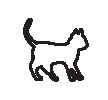
\includegraphics[width=350pt, height=200pt]{chapters/chapter1/figures/cat.eps}
%%\centerline{\epsfig{/Chapters/chapter1/figures/cat.eps,width=.8\textheight,height=.4\textwidth}}
\caption[List of figure caption goes here]{Figure caption goes here.}
\end{figure}



\begin{figure}[htb]
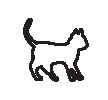
\includegraphics[width=200pt, height=200pt]{chapters/chapter1/figures/cat}
%%\centerline{\epsfig{figure=cat.eps,width=.5\textheight,height=.4\textwidth}}
\caption[Short figure caption]{Figure caption goes here. Figure caption goes here.
Figure caption goes here. Figure caption goes here. Figure caption goes here.
Figure caption goes here.}
\end{figure}





\begin{figure}
\begin{center}
\subfigure[\label{f8a}]{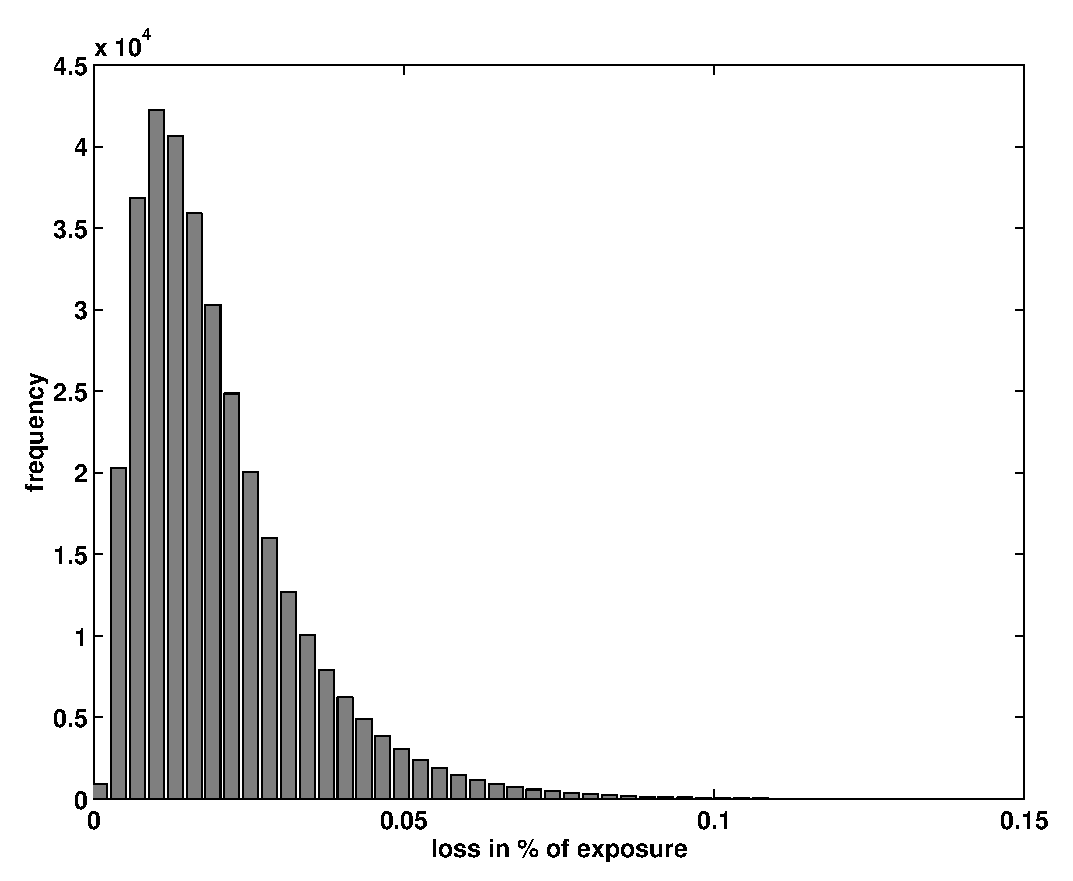
\includegraphics[angle=90,width=7cm,height=7cm,angle=-90]{chapters/chapter1/figures/Histogram.eps}}
\subfigure[\label{f8b}]{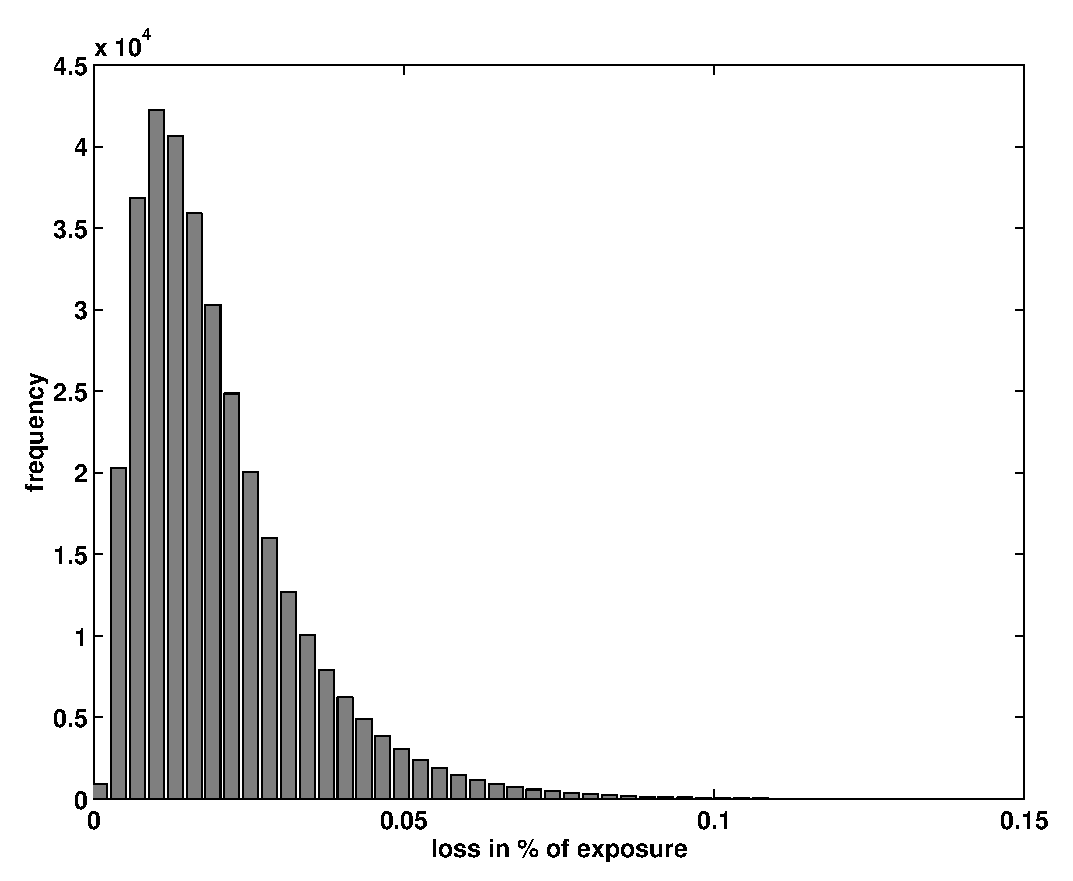
\includegraphics[angle=90,width=7cm,height=7cm,angle=-90]{chapters/chapter1/figures/Histogram.eps}}
\end{center}
\caption[The bar charts depict the different risk contributions]{The bar charts depict the different risk contributions (top: 99\% quantile, bottom: 99.9\% quantile) of the business areas of a bank. The black bars
are based on a Var/Covar approach, the white ones correspond to shortfall risk.}
\end{figure}

\subsubsection{H3 A component part }
A component part for an electronic item is
manufactured at one of three \cite{mardia1979ma} different factories, and then delivered to
the main assembly line.Of the total number supplied, factory A supplies
50\%, factory B 30\%, and factory C 20\%. Of the components
manufactured at factory A, 1\% are faulty and the corresponding
proportions for factories B and C are 4\% and 2\% respectively. A
component is picked at random from the assembly line. What is the
probability that it is faulty?


A fundamental notion \cite{yao2002can} is that of a\index{subspace}\index{vector
space!subspace of} subspace of $F^n$. Let $V$ be a nonempty subset of
$F^n$. Then $V$ is a {\it subspace} of $F^n$ provided $V$ is closed
under vector addition and scalar multiplication, that is,
\begin{enumerate}
\item[\rm (a)] For all $u$ and $v$ in $V$, $u+v$ is
also in $V$.
\item[\rm (b)] For all $u$ in $V$ and $c$ in $F$, $cu$ is
in $V$.
\end{enumerate}
Let $u$ be in the subspace $V$. Because $0u=0$,
it follows that the zero vector is in $V$. Similarly, $-u$ is in $V$
for all $u$ in $V$. A simple example of a subspace of $F^n$ is the set
of all vectors $(0,a_2,\ldots,a_n)$ with first coordinate equal to 0.
The zero vector itself is a subspace.

\begin{definition}\label{1def:linearcomb}{\rm
Let $u^{(1)},u^{(2)},\ldots,u^{(m)}$ be vectors in $F^n$, and let
$c_1,c_2,\ldots,c_m$ be scalars. Then the vector
\[c_1u^{(1)}+c_2u^{(2)}+\cdots+c_mu^{(m)}\]
is called a {\it linear combination} \index{linear combination} of $u^{(1)},u^{(2)},\ldots,u^{(m)}$.
If $V$ is a subspace of $F^n$, then $V$ is closed under vector addition and
scalar multiplication, and it follows easily by induction that a
linear combination of vectors in $V$ is also a vector in $V$. Thus
{\it subspaces
are closed under linear combinations}; in fact, this can be taken as the
defining property of subspaces.
The vectors $u^{(1)},u^{(2)},\ldots,u^{(m)}$ {\it span} $V$ \index{spanning set}
(equivalently, form a {\it spanning set} of $V$) provided every vector in
$V$
is a linear combination of $u^{(1)},u^{(2)},\ldots,u^{(m)}$. The zero
vector can be written as a linear combination of
$u^{(1)},u^{(2)},\ldots,u^{(m)}$ with all scalars equal to 0; this is a
{\it trivial linear combination}.\index{linear combination!trivial} The vectors
$u^{(1)},u^{(2)},\ldots,u^{(m)}$ are {\it linearly dependent} provided
there are scalars $c_1,c_2,\ldots,c_m$, not all of which are zero, such
that
\[c_1u^{(1)}+c_2u^{(2)}+\cdots+c_mu^{(m)}=0,\]
that is, the zero vector can be written as a {\it nontrivial linear \index{linear combination!nontrivial}
combination} of $u^{(1)},u^{(2)},\ldots,u^{(m)}$.
For example, the vectors $(1,4), (3,-1)$, and $(3,5)$ in $\Re^2$ are
linearly
dependent since
\[3(1,4)+1(3,-2)-2(3,5)=(0,0).\] Vectors are {\it linearly independent} provided  they are not linearly dependent.\index{linearly independent}
The vectors
$u^{(1)},u^{(2)},\ldots,u^{(m)}$ are a {\it basis} \index{basis} of $V$ provided they are
linearly independent and span $V$.
By an {\it ordered basis} \index{basis!ordered} we mean a basis in which the vectors of the basis are listed
in a specified order; to indicate that we have an ordered basis we write
$(u^{(1)},u^{(2)},\ldots,u^{(m)})$.
A spanning set $S$ of $V$ is a \index{spanning set!minimal} {\it minimal spanning set of $V$} provided that
each set
of vectors obtained from $S$ by removing a vector is not a spanning set
for $V$.
A linearly independent set $S$ of vectors of $V$ is a {\it maximal linearly \index{linearly independent!maximal}
independent set of vectors of $V$} provided that for each vector $w$ of
$V$ that
is not in $S$, $S\cup\{w\}$ is  linearly dependent (when this happens,
$w$ must be  a linear combination of the vectors in
$S$).\hfill{$\Box$}
}\end{definition}

In addition to matrix addition, subtraction, and multiplication, there is
one additional operation that we define now. It's perhaps the simplest of
them all. Let $A=[a_{ij}]$ be an $m$ by $n$ matrix and let $c$ be a
number \cite{hyvarinen2001ica}. Then the matrix $c\cdot A$, or simply $cA$, is the $m$ by $n$
matrix obtained by multiplying each entry of $A$ by $c$:
\[c A=[ca_{ij}].\]\index{matrix!scalar multiplication} \index{matrix!scalar multiple of}
The matrix $c A$ is called a {\it scalar multiple} of $A$.

\begin{VT1}

\VH{Think About It...}

Commonly thought of as the first modern computer, ENTAC was built in 1944. It took up more space than an 18-wheeler's
tractor trailer and weighed more than 17 Chevrolet Camaros. It consumed 140,000 watts of electricity while executing
up to 5,000 basic arithmetic operations per second. One of today's popular microprocessors, the 486, is built on a
tiny piece of silicon about the size of a dime.

\VT
With the continual expansion of capabilities, computing power will eventually exceed the capacity for human
comprehension or human control.

\VTA{The Information Revolution}{Business Week}
\end{VT1}


\section{Glossary}
\begin{Glossary}
\item[360 Degree Review] Performance review that includes feedback from superiors, peers, subordinates, and clients.
\item[Abnormal Variation] Changes in process performance that cannot be accounted for by typical day-to-day variation. Also referred to as
non-random variation.
\item[Acceptable Quality Level (AQL)] The minimum number of parts that must comply with quality standards, usually stated as a percentage.
\item[Activity] The tasks performed to change inputs into outputs.
\item[Adaptable] An adaptable process is designed to maintain effectiveness and efficiency as requirements change. The process is
deemed adaptable when there is agreement among suppliers, owners, and customers that the process will meet
requirements throughout the strategic period.
\end{Glossary}




\choice{}{%This chapter was modified on 4/2/97.
%\setcounter{chapter}{1}
\chapter{Continuous Probability Densities}\label{chp 2}

\section{Simulation of Continuous Probabilities}\label{sec 2.1}

In this section we shall show how we can use computer simulations for
experiments that have a whole continuum\index{continuum} of possible outcomes.

\subsection*{Probabilities}

\begin{example}\label{exam 2.1.1}
We begin by constructing a spinner\index{spinner}, which consists of a circle of \emx {unit 
circumference} and a pointer as shown in Figure~\ref{fig 2.05}.  We pick a point on
the circle and label it 0, and then label every other point on the circle with the
distance, say $x$, from 0 to that point, measured counterclockwise.  The experiment consists of
spinning the pointer and recording the label of the point at the tip of the
pointer.  We let the random variable $X$ denote the value of this outcome.   The sample space
is clearly the interval $[0, 1)$.  We would like to construct a probability model in which
each outcome is equally likely to occur.
\par
If we proceed as we did in Chapter~\ref{chp 1} for experiments with a finite number of
possible outcomes, then we must assign the probability 0 to each outcome, since otherwise,
the sum of the probabilities, over all of the possible outcomes, would not equal 1.  (In
fact, summing an uncountable number of real numbers is a tricky business; in particular, 
in order for such a sum to have any meaning, at most countably many of the summands can be
different than 0.)  However, if all of the assigned probabilities are 0, then the sum is 0,
not 1, as it should be.
\putfig{2truein}{PSfig2-12arc}{A spinner.}{fig 2.05}
\par
In the next section, we will show how to construct a probability model in this situation. 
At present, we will assume that such a model can be constructed.  We will also assume that
in this model, if $E$ is an arc of the circle, and $E$ is of length $p$, then the model 
will assign the probability $p$ to $E$.  This means that if the pointer is spun, the
probability that it ends up pointing to a point in $E$ equals $p$, which is certainly a
reasonable thing to expect.
\par
To simulate this experiment on a computer is an easy matter.  Many computer software
packages have a function which returns a random real number in the interval $[0, 1]$. 
Actually, the returned value is always a rational number, and the values are determined by
an algorithm, so a sequence of such values is not truly random.  Nevertheless,
the sequences produced by such algorithms behave much like theoretically random sequences,
so we can use such sequences in the simulation of experiments.  On occasion, we will need
to refer to such a function.  We will call this function $rnd$\index{rnd}.
\end{example}

\subsection*{Monte Carlo Procedure and Areas}

It is sometimes desirable to estimate quantities whose exact values are difficult or 
impossible to calculate exactly.  In some of these cases, a procedure involving chance, called 
a \emx {Monte Carlo procedure}, can be used to provide such an estimate.

\begin{example}\label{exam 2.1.2}
In this example we show how simulation can be used to estimate areas
\index{area, estimation of} of
plane figures.  Suppose that we program our computer to provide a pair $(x,y)$ or
numbers, each chosen independently at random from the interval $[0,1]$.  Then
we can interpret this pair $(x,y)$ as the coordinates of a point chosen \emx {at
random} from the unit square.  Events are subsets of the unit square. 
Our experience with Example~\ref{exam 2.1.1} suggests that the point is
equally likely to fall in subsets of equal area.  Since the total area of the
square is 1, the probability of the point falling in a specific subset $E$ of
the unit square should be equal to its area.  Thus, we can estimate the area of
any subset of the unit square by estimating the probability that a point chosen
at random from this square falls in the subset.
\par
We can use this method to estimate the area of the region $E$ under the curve
$y = x^2$ in the unit square (see Figure~\ref{fig 2.3}).  We choose a large number of
points $(x,y)$ at random and record what fraction of them fall in the region $E
= \{\,(x,y):y \leq x^2\,\}$.
\par
The program {\bf MonteCarlo}\index{MonteCarlo (program)} will carry out this experiment for us. 
Running this program for 10{,}000 experiments gives an estimate of .325 (see
Figure~\ref{fig 2.4}).                     

\putfig{3truein}{PSfig2-3}{Area under $y = x^2.$}{fig 2.3}

From these experiments we would estimate the area to be about 1/3.  Of course,
for this simple region we can find the exact area by calculus.  In fact,
$$
\mbox{Area of}\ E = \int_0^1 x^2\,dx = \frac13\ .
$$
We have remarked in Chapter~\ref{chp 1} that,
when we simulate an experiment of this type $n$ times to estimate a probability, we can 
expect the answer to be in error by at most $1/\sqrt n$ at least 95 percent of the
time. For 10{,}000 experiments we can expect an accuracy of 0.01, and our simulation
did achieve this accuracy.

\putfig{3truein}{PSfig2-4}{Computing the area by simulation.}{fig 2.4}  

This same argument works for any region $E$ of the unit square.  For example,
suppose $E$ is the circle with center $(1/2,1/2)$ and radius 1/2. 
Then the probability that our random point $(x,y)$ lies inside the circle
is equal to the area of the circle, that is,
$$
P(E) = \pi{\Bigl(\frac{1}{2}\Bigr)}^2 = \frac{\pi}{4}\ .
$$
If we did not know the value of $\pi$, we could estimate\index{$\pi$, estimation of|(} 
the value by performing this
experiment a large number of times!
\end{example}

The above example is not the only way of estimating the value of $\pi$ by a
chance experiment.  Here is another way, discovered by Buffon.\footnote{G. L.
Buffon, in ``Essai d'Arithm\'etique Morale," \emx {Oeuvres Compl\`etes de
Buffon avec Supplements,} tome~iv, ed. Dum\'enil (Paris, 1836).}

\subsection*{Buffon's Needle}\index{BUFFON, G. L.}
\index{Buffon's needle|(}

\begin{example}\label{exam 2.1.3}
Suppose that we take a card table and draw across the top surface a set of parallel
lines a unit distance apart.  We then drop a common needle of unit length at
random on this surface and observe whether or not the needle lies across one of
the lines.  We can describe the possible outcomes of this experiment by
coordinates as follows:  Let $d$ be the distance from the center of the needle
to the nearest line.  Next, let $L$ be the line determined by the needle, and define $\theta$
as the acute angle that the line $L$ makes with the set of parallel lines.  (The reader should
certainly be wary of this description of the sample space.  We are attempting to coordinatize
a set of line segments.  To see why one must be careful in the choice of coordinates, see
Example~\ref {exam 2.1.5}.)  Using this description, we have $0
\leq d \leq 1/2$, and $0 \leq
\theta \leq \pi/2$.  Moreover, we see that the needle lies across the
nearest line if and only if the hypotenuse of the triangle (see Figure~\ref
{fig 2.6}) is less than half the length of the needle, that is, 
$$
\frac d{\sin\theta} < \frac12\ .
$$

\putfig{4.5truein}{PSfig2-6}{Buffon's experiment.}{fig 2.6}

Now we assume that when the needle drops, the pair $(\theta,d)$ is chosen at
random from the rectangle $0 \leq \theta \leq \pi/2$, $0 \leq d \leq 1/2$.  We
observe whether the needle lies across the nearest line (i.e., whether $d \leq
(1/2)\sin\theta$).  The probability of this event $E$ is the fraction of
the area of the rectangle which lies inside $E$ (see Figure~\ref{fig 2.7}).             
Now the area of the rectangle is $\pi/4$, while the area of $E$ is
$$
\mbox{Area} = \int_0^{\pi/2}\frac12\sin\theta\,d\theta = \frac 12\ .
$$
Hence, we get
$$
P(E) = \frac{1/2}{\pi/4} = \frac2\pi\ .
$$

\putfig{3.5truein}{PSfig2-7}
{Set $E$ of pairs $(\theta, d)$ with $d < {\frac{1}{2}} \sin \theta$.}{fig 2.7}

The program {\bf BuffonsNeedle}\index{BuffonsNeedle (program)} simulates this experiment.  In
Figure~\ref{fig 2.8}, we show the position of every 100th needle in a run of the program in
which 10{,}000 needles were ``dropped."  Our final estimate for $\pi$ is 3.139.  While this was
within 0.003 of the  true value for $\pi$ we had no right to expect such accuracy.  The reason
for this is that our simulation estimates $P(E)$.  While we can expect this estimate to be in
error by at most 0.001, a small error in $P(E)$ gets magnified when we use this to compute $\pi =
2/P(E)$.  Perlman\index{PERLMAN, M. D.} and Wichura\index{WICHURA, M. J.}, in their article
``Sharpening Buffon's Needle,"\footnote{M. D. Perlman and M. J. Wichura, ``Sharpening
Buffon's Needle," \emx {The American Statistician,} vol.~29, no.~4 (1975), pp.~157--163.}
show that we can expect to have an error of not more than $5/\sqrt n$ about 95 percent of
the time.  Here $n$ is the number of needles dropped.  Thus for 10{,}000 needles we should
expect an error of no more than 0.05, and that was the case here.  We see that a large
number of experiments is necessary to get a decent estimate for
$\pi$.\index{$\pi$, estimation of|)}
\index{Buffon's needle|)}
\end{example}

\putfig{4truein}{PSfig2-8}{Simulation of Buffon's needle experiment.}{fig 2.8}

In each of our examples so far, events of the same size are equally likely. 
Here is an example where they are not.  We will see many other such examples later.
\begin{example}\label{exam 2.1.4.5}
Suppose that we choose two random real numbers in $[0,1]$ and add them together.  Let $X$
be the sum.  How is $X$ distributed?
\par
To help understand the answer to this question, we can use the program {\bf
Areabargraph}\index{Areabargraph (program)}.  This  program produces a bar graph with the
property that on each interval, the \emx {area},  rather than the height, of the bar is equal to
the fraction of outcomes that fell in the corresponding interval.  We have carried out this
experiment 1000 times; the data is shown in Figure~\ref{fig 2.8.5}.  It appears that the
function defined by
$$f(x) = \left \{ \begin{array}{ll}
                  x,   & \mbox{if $0 \le x \le 1$,}  \\
                  2-x, & \mbox{if $1 < x \le 2$} 
                  \end{array}
         \right.
$$
fits the data very well.  (It is shown in the figure.)  In the next section, we will see 
that this function is the ``right" function. By this we mean that if $a$ and $b$ are any
two real numbers between $0$ and $2$, with $a \le b$, then we can use this function to
calculate the probability that
$a \le X \le b$.  To understand how this calculation might be performed, we again consider
Figure~\ref{fig 2.8.5}.  Because of the way the bars were constructed, the sum of the areas of the
bars corresponding to the interval $[a, b]$ approximates the probability that $a \le X 
\le b$.  But the sum of the areas of these bars also approximates the integral
$$\int_a^b f(x)\,dx\ .$$  This suggests that for an experiment with a continuum of possible outcomes, 
if we find a function with the above property, then we will be able to use it to calculate
probabilities.  In the next section, we will show how to determine the function
\linebreak[4]$f(x)$.
\putfig{3.5truein}{PSfig2-8-5}{Sum of two random numbers.}{fig 2.8.5}
\end{example}

\begin{example}\label{exam 2.1.4.6}
Suppose that we choose 100 random numbers in $[0, 1]$, and let $X$ represent their sum.  
How is $X$ distributed?  We have carried out this experiment 10000 times; the results are
shown in  Figure~\ref{fig 2.8.6}.  It is not so clear what function fits the bars in this
case.  It turns out that the type of function which does the job is called a \emx {normal
density}\index{normal density} function.  This type of function is sometimes referred to as a
``bell-shaped"\index{bell-shaped} curve.  It is among the most important functions in the
subject of probability, and will be formally defined in Section~\ref{sec 5.2}
of Chapter~\ref{chp 5}.
\putfig{3.5truein}{PSfig2-8-6}{Sum of 100 random numbers.}{fig 2.8.6}
\end{example}
\par
Our last example explores the fundamental question of how probabilities are
assigned.

\subsection*{Bertrand's Paradox}\index{Bertrand's paradox|(}

\begin{example}\label{exam 2.1.5} 
A chord of a circle is a line segment both of whose endpoints lie on the
circle.  Suppose that a chord is drawn \emx {at random}\index{chord, random} in a unit circle. 
What is the probability that its length exceeds $\sqrt 3$?

Our answer will depend on what we mean by \emx {random,} which
will depend, in turn, on what we choose for coordinates.  The sample space
$\Omega$ is the set of all possible chords in the circle.  To find coordinates
for these chords, we first introduce a rectangular coordinate system with
origin at the center of the circle (see Figure~\ref{fig 2.10}).  We note that a chord
of a circle is perpendicular to the radial line containing the midpoint of the
chord.  We can describe each chord by giving:
 
\begin{enumerate}
\item The rectangular coordinates $(x,y)$ of the midpoint $M$, or
\item The polar coordinates $(r,\theta)$ of the midpoint $M$, or
\item The polar coordinates $(1,\alpha)$ and $(1,\beta)$ of the endpoints $A$
and $B$.
 
\end{enumerate}
In each case we shall interpret \emx {at random} to mean: choose these
coordinates at random.

We can easily estimate this probability by computer simulation.  In programming this 
simulation, it is convenient to include certain simplifications, which we describe in turn:

\putfig{2.5truein}{PSfig2-10}{Random chord.}{fig 2.10}

\begin{enumerate}
\item To simulate this case, we choose values for $x$ and $y$ from $[-1,1]$ at
random.  Then we check whether $x^2 + y^2 \leq 1$.  If not, the point $M =
(x,y)$ lies outside the circle and cannot be the midpoint of any chord, and we
ignore it.  Otherwise, $M$ lies inside the circle and is the midpoint of a
unique chord, whose length $L$ is given by the formula:
$$
L = 2\sqrt{1 - (x^2 + y^2)}\ .
$$
\item To simulate this case, we take account of the fact that any rotation of
the circle does not change the length of the chord, so we might as well assume
in advance that the chord is horizontal.  Then we
choose $r$ from $[-1,1]$ at random, and compute the length of the resulting
chord with midpoint $(r,\pi/2)$ by the formula:
$$
L = 2\sqrt{1 - r^2}\ .
$$
\item To simulate this case, we assume that one endpoint, say $B$, lies at
$(1, 0)$ (i.e., that $\beta = 0$).  Then we choose a value for $\alpha$ from
$[0,2\pi]$ at random and compute the length of the resulting chord, using the
Law of Cosines, by the formula:
$$
L = \sqrt{2 - 2\cos\alpha}\ .
$$
\end{enumerate}

The program {\bf BertrandsParadox}\index{BertrandsParadox (program)} carries out this
simulation.  Running this program produces the results shown in Figure~\ref{fig 2.11}.  In the
first  circle in this figure, a smaller circle has been drawn.  Those chords which intersect this
smaller circle have length at least $\sqrt 3$.  In the second circle in the figure, the
vertical line intersects all chords of length at least $\sqrt 3$.  In the third circle,
again the vertical line intersects  all chords of length at least $\sqrt 3$.

In each case we run the experiment a large number of times and record the
fraction of these lengths that exceed $\sqrt 3$.  We have printed the results
of every 100th trial up to 10{,}000 trials.

\putfig{4.5truein}{PSfig2-11}{Bertrand's paradox.}{fig 2.11}

It is interesting to observe that these fractions are \emx {not} the same in
the three cases; they depend on our choice of coordinates.  This phenomenon was
first observed by Bertrand, and is now known as \emx {Bertrand's
paradox.}\index{BERTRAND, J.}\footnote{J. Bertrand, \emx {Calcul des Probabilit\'es}
(Paris: Gauthier-Villars, 1889).}  It is actually not a paradox at all; it is merely a
reflection of the fact that different choices of coordinates will lead to
different assignments of probabilities.  Which assignment is ``correct"
depends on what application or interpretation of the model one has in mind.
\par
One can imagine a real experiment involving throwing long straws at a circle
drawn on a card table.  A ``correct" assignment of coordinates should not depend on 
where the circle lies on the card table, or where the card table sits in the room. 
Jaynes\index{JAYNES, E. T.}\footnote{E. T. Jaynes, ``The Well-Posed Problem," in \emx
{Papers on Probability, Statistics and Statistical Physics,} R.~D.~Rosencrantz, ed.
(Dordrecht: D.~Reidel, 1983), pp.~133--148.} has shown that the only assignment which
meets this requirement is (2).  In this sense, the assignment (2) is the natural, or
``correct" one (see Exercise~\ref{exer
2.1.11}).                                             
\par
We can easily see in each case what the true probabilities are if we note that
$\sqrt 3$ is the length of the side of an inscribed equilateral triangle. 
Hence, a chord has length $L > \sqrt 3$ if its midpoint has distance $d < 1/2$
from the origin (see Figure~\ref{fig 2.10}).  The following calculations determine
the probability that $L > \sqrt 3$ in each of the three cases.
\begin{enumerate}
\item $L > \sqrt 3$ if$(x,y)$ lies inside a circle of radius 1/2, which occurs with 
probability
$$
p = \frac{\pi(1/2)^2}{\pi(1)^2} = \frac14\ .
$$
\item $L > \sqrt 3$ if $|r| < 1/2$, which occurs with probability
$$
\frac{1/2 - (-1/2)}{1 - (-1)} = \frac12\ .
$$
\item $L > \sqrt 3$ if $2\pi/3 < \alpha < 4\pi/3$, which occurs with probability
$$
\frac{4\pi/3 - 2\pi/3}{2\pi - 0} = \frac13\ .
$$
\end{enumerate}
We see that our simulations agree quite well with these theoretical values.\index{Bertrand's
paradox|)}
\end{example}

\subsection*{Historical Remarks}

G.~L.~Buffon\index{BUFFON, G. L.|(} (1707--1788) was a natural scientist in the eighteenth
century who applied probability to a number of his investigations.  His work is found in
his monumental 44-volume \emx {Histoire Naturelle} and its
supplements.\footnote{G.~L.~Buffon, \emx {Histoire Naturelle, Generali et
Particular avec le Descripti\'on du Cabinet du Roy,} 44~vols. (Paris:
L`Imprimerie Royale, 1749--1803).}  For example, he presented a number of
mortality tables and used them to compute, for each age group, the expected
remaining lifetime.  From his table he observed: the expected remaining
lifetime of an infant of one year is 33 years, while that of a man of 21 years
is also approximately 33 years.  Thus, a father who is not yet 21 can hope to
live longer than his one year old son, but if the father is 40, the odds are
already 3 to 2 that his son will outlive him.\footnote{G.~L.~Buffon, ``Essai
d'Arithm\'etique Morale," p.~301.}
\par
Buffon wanted to show that not all probability calculations rely only on
algebra, but that some rely on geometrical calculations.  One such problem
was his famous ``needle problem"\index{Buffon's needle|(} as discussed in this
chapter.\footnote{ibid., pp.~277--278.}  In his original formulation, Buffon describes a game
in which two gamblers drop a loaf of French bread on a wide-board floor and bet on
whether or not the loaf falls across a crack in the floor.  Buffon asked: what
length $L$ should the bread loaf be, relative to the width $W$ of the
floorboards, so that the game is fair.  He found the correct answer ($L =
(\pi/4)W$) using essentially the methods described in this chapter.  He also
considered the case of a checkerboard floor, but gave the wrong answer in this
case.  The correct answer was given later by Laplace.\index{BUFFON, G. L.|)}\index{LAPLACE,
P. S.}
\par
The literature contains descriptions of a number of experiments that were
actually carried out to estimate $\pi$ by this method of dropping needles.
N.~T.~Gridgeman\index{GRIDGEMAN, N. T.}\footnote{N.~T.~Gridgeman, ``Geometric Probability and
the Number $\pi$" \emx {Scripta Mathematika,} vol.~25, no.~3, (1960),
pp.~183--195.} discusses the experiments shown in Table~\ref{table 2.1}.
\begin{table}
\centering
$$ 
\begin{tabular}{llrll}
               &  Length of              &  Number of       &  Number of      &  Estimate  \\
Experimenter   &  needle                 & casts\,\,\,\,\,\,&  crossings      &  for $\pi$  \\ \hline
Wolf, 1850     &  \hspace{.073in}.8      & 5000\,\,\,\,\,\, &  2532                  & 3.1596      \\
Smith, 1855    &  \hspace{.073in}.6      & 3204\,\,\,\,\,\, &  1218.5                & 3.1553      \\
De Morgan, c.1860& 1.0                   & 600\,\,\,\,\,\,  &  \hspace{.075in}382.5  & 3.137       \\
Fox, 1864      &  \hspace{.078in}.75     & 1030\,\,\,\,\,\, &  \hspace{.075in}489    & 3.1595      \\
Lazzerini, 1901&  \hspace{.078in}.83     & 3408\,\,\,\,\,\, &  1808                  & 3.1415929   \\
Reina, 1925    &  \hspace{.083in}.5419   & 2520\,\,\,\,\,\, &  \hspace{.075in}869    & 3.1795  \\ \hline
\end{tabular}
$$
\caption{Buffon needle experiments to estimate $\pi$.}
\label{table 2.1}
\end{table}
(The halves for the number of crossing comes from a compromise when it could
not be decided if a crossing had actually occurred.)  He observes, as we have,
that 10{,}000 casts could do no more than establish the first decimal place of
$\pi$ with reasonable confidence.  Gridgeman points out that, although none of
the experiments used even 10{,}000 casts, they are surprisingly good, and in some
cases, too good.  The fact that the number of casts is not always a round number
would suggest that the authors might have resorted to clever stopping to get a
good answer.  Gridgeman comments that Lazzerini's estimate turned out to agree
with a well-known approximation to $\pi$, $355/113 = 3.1415929$, discovered by
the fifth-century Chinese mathematician, Tsu Ch'ungchih.  Gridgeman says that
he did not have Lazzerini's original report, and while waiting for it (knowing
only the needle crossed a line 1808 times in 3408 casts) deduced that the
length of the needle must have been 5/6.  He calculated this from Buffon's
formula, assuming $\pi = 355/113$:
$$
L = \frac{\pi P(E)}2 =
\frac12\left(\frac{355}{113}\right)\left(\frac{1808}{3408}\right) = \frac56 =
.8333\ .
$$
Even with careful planning one would have to be extremely lucky to be able to
stop so cleverly\index{Buffon's needle|)}.
\par
The second author likes to trace his interest in probability theory to the Chicago
World's Fair\index{Chicago World's Fair} of 1933 where he observed a mechanical device dropping
needles and displaying the ever-changing estimates for the value of $\pi$.  (The first author
likes  to trace his interest in probability theory to the second author.)

\exercises
\begin{LJSItem}

\istar\label{exer 2.1.1} In the spinner problem (see Example~\ref{exam 2.1.1})   
divide the unit circumference into three arcs of length 1/2, 1/3, and 1/6. 
Write a program to simulate the spinner experiment 1000 times and print out what
fraction of the outcomes fall in each of the three arcs.  Now plot a bar graph
whose bars have width 1/2, 1/3, and 1/6, and areas equal to the corresponding
fractions as determined by your simulation.  Show that the heights of the bars
are all nearly the same.

\i\label{exer 2.1.2} Do the same as in Exercise~\ref{exer 2.1.1}, 
but divide the unit
circumference into five arcs of length 1/3, 1/4, 1/5, 1/6, and 1/20.

\i\label{exer 2.1.3} Alter the program {\bf MonteCarlo} to estimate the area of the
circle of radius 1/2 with center at $(1/2,1/2)$ inside the unit square by
choosing 1000 points at random.  Compare your results with the true value of
$\pi/4$.  Use your results to estimate the value of $\pi$.  How accurate is
your estimate?

\i\label{exer 2.1.4} Alter the program {\bf MonteCarlo} to
estimate the area under the graph of $y = \sin\pi x$ inside the unit square by
choosing 10{,}000 points at random.  Now calculate the true value of this
area and use your results to estimate the value of $\pi$.  How accurate is your estimate?

\i\label{exer 2.1.5} Alter the program {\bf MonteCarlo} to estimate the area under the
graph of $y = 1/(x + 1)$ in the unit square in the same way as in Exercise~\ref
{exer 2.1.4}.   Calculate the true value of this area and use
your simulation results to estimate the value of $\log 2$.  How accurate is your
estimate?

\i\label{exer 2.1.6} To simulate the Buffon's needle\index{Buffon's needle} problem we choose
independently the distance~$d$ and the angle $\theta$ at random, with $0 \leq d
\leq 1/2$ and $0 \leq \theta \leq \pi/2$, and check whether $d \leq
(1/2)\sin\theta$.  Doing this a large number of times, we estimate $\pi$ as
$2/a$, where $a$ is the fraction of the times that $d \leq (1/2)\sin\theta$. 
Write a program to estimate $\pi$ by this method.  Run your program several
times for each of 100, 1000, and 10{,}000 experiments.  Does the accuracy of the
experimental approximation for $\pi$ improve as the number of experiments
increases?

\i\label{exer 2.1.7} For Buffon's needle problem\index{Buffon's needle}, Laplace\index{LAPLACE,
P. S.}\footnote{P. S. Laplace, \emx {Th\'eorie Analytique des Probabilit\'es} (Paris: Courcier,
1812).} considered a grid with \emx {horizontal} and \emx {vertical} lines one unit apart.  He
showed that the probability that a needle of length $L \leq 1$ crosses at least
one line is
$$
p = \frac{4L - L^2}\pi\ .
$$
To simulate this experiment we choose at random an angle $\theta$ between
0~and $\pi/2$ and independently two numbers $d_1$ and $d_2$ between 0 and
$L/2$. 
(The two numbers represent the distance from the center of the needle to the
nearest horizontal and vertical line.)  The needle crosses a line if either
$d_1 \leq (L/2)\sin\theta$ or $d_2 \leq (L/2)\cos\theta$.  We do this a large
number of times and estimate $\pi$ as
$$
\bar \pi = \frac{4L - L^2}a\ ,
$$
where $a$ is the proportion of times that the needle crosses at least one
line.  Write a program to estimate $\pi$ by this method, run your program for
100, 1000, and 10{,}000 experiments, and compare your results with Buffon's
method described in Exercise~\ref{exer 2.1.6}.    
(Take $L = 1$.)

\i\label{exer 2.1.8} A long needle\index{Buffon's needle} of length $L$ much bigger than 1 is
dropped on a grid with horizontal and vertical lines one unit apart.  We will see 
(in Exercise~\ref{sec 6.3}.\ref{exer 6.3.29}) that the average number $a$ of lines crossed
is approximately
$$
a = \frac{4L}\pi\ .
$$
To estimate $\pi$ by simulation, pick an angle $\theta$ at random between 0 and
$\pi/2$ and compute $L\sin\theta + L\cos\theta$.  This may be used for the
number of lines crossed.  Repeat this many times and estimate $\pi$ by
$$
\bar \pi = \frac{4L}a\ ,
$$
where $a$ is the average number of lines crossed per experiment.  Write a
program to simulate this experiment and run your program for the number of
experiments equal to 100, 1000, and 10{,}000.  Compare your results with the
methods of Laplace or Buffon for the same number of experiments.  (Use $L = 100$.)

\medbreak\noindent
The following exercises involve experiments in which not all outcomes are
equally likely.  We shall consider such experiments in detail in the next
section, but we invite you to explore a few simple cases here.

\i\label{exer 2.1.9} A large number of waiting time problems have an
\emx {exponential distribution}\index{exponential density}\index{density function!exponential}
of outcomes.  We shall see (in Section~\ref{sec 5.2})  that such outcomes are simulated by
computing
$(-1/\lambda)\log(\mbox{rnd})$, where $\lambda > 0$.  For waiting times produced
in this way, the average waiting time is $1/\lambda$.  For example, the times
spent waiting for a car to pass on a highway, or the times between emissions of particles 
from a radioactive source, are simulated by a sequence of random numbers, each of
which is chosen by computing $(-1/\lambda)\log(\mbox{rnd})$, where $1/\lambda$ is
the average time between cars or emissions.  Write a program to simulate the
times between cars when the average time between cars is 30 seconds.  Have your
program compute an area bar graph for these times by breaking the time interval from
0 to 120 into 24 subintervals.  On the same pair of axes, plot the function
$f(x) = (1/30)e^{-(1/30)x}$.  Does the function fit the bar graph well?

\i\label{exer 2.1.10.5} In Exercise~\ref{exer 2.1.9},
the distribution came ``out of a hat."  In this problem, we will again consider an
experiment whose outcomes are not equally likely.  We will determine a function
$f(x)$ which can be used to determine the probability of certain events. 
Let $T$ be the right triangle in the plane with vertices at the points $(0, 0),\ (1, 0),$
and $(0,1)$.  The experiment consists of picking a point at random in the interior
of $T$, and recording only the $x$-coordinate of the point.  Thus, the sample space is
the set $[0,1]$, but the outcomes do not seem to be equally likely.  We can simulate this
experiment by asking a computer to return two random real numbers in $[0,
1]$, and recording the first of these two numbers if their sum is less than 1. 
Write this program and run it for 10{,}000 trials.  Then make a bar graph of the
result, breaking the interval $[0, 1]$ into 10 intervals.  Compare the bar graph with the
function $f(x) = 2 - 2 x$.  Now show that there is a constant $c$ such that the
height of $T$ at the $x$-coordinate value $x$ is $c$ times $f(x)$ for every $x$ in
$[0, 1]$.  Finally, show that  $$\int_0^1 f(x)\,dx = 1\ .$$
How might one use the function $f(x)$ to determine the probability that the
outcome is between $.2$ and $.5$?

\i\label{exer 2.1.11} Here is another way to pick a chord\index{chord, random} \emx {at random}
on the circle of unit radius.  Imagine that we have a card table whose sides are of
length 100.  We place coordinate axes on the table in such a way that each side of
the table is parallel to one of the axes, and so that the center of the table is the
origin.  We now place a circle of unit radius on the table so that the center of the 
circle is the origin.  Now pick out a point
$(x_0,y_0)$ at random in the square, and an angle
$\theta$ at random in the interval $(-\pi/2,\pi/2)$.  Let $m = \tan\theta$. 
Then the equation of the line passing through $(x_0,y_0)$ with slope $m$ is
$$
y = y_0 + m(x - x_0)\ ,
$$
and the distance of this line from the center of the circle (i.e., the origin)
is
$$
d = \left|\frac{y_0 - mx_0}{\sqrt{m^2 + 1}}\right|\ .
$$

We can use this distance formula to check whether the line intersects the
circle (i.e., whether $d < 1$).  If so, we consider the resulting chord a {\em
random} chord.  This describes an experiment of dropping a long straw at
random on a table on which a circle is drawn.

Write a program to simulate this experiment 10000 times and estimate the
probability that the length of the chord is greater than $\sqrt3$.  How does
your estimate compare with the results of Example~\ref{exam 2.1.5}?  
\end{LJSItem}


\section{Continuous Density Functions}\label{sec 2.2}

In the previous section we have seen how to simulate experiments with a whole
continuum of possible outcomes and have gained some experience in thinking
about such experiments.  Now we turn to the general problem of assigning
probabilities to the outcomes and events in such experiments.  We shall
restrict our attention here to those experiments whose sample space can be
taken as a suitably chosen subset of the line, the plane, or some other
Euclidean space.  We begin with some simple examples.

\subsection*{Spinners}

\begin{example}\label{exam 2.2.1}
The spinner\index{spinner} experiment described in Example~\ref{exam 2.1.1} has the interval
$[0, 1)$ as  the set of possible outcomes.  We would like to construct a probability model in
which  each outcome is equally likely to occur.  We saw that in such a model, it is necessary
to assign the probability 0 to each outcome.  This does not at all mean that the probability
of \emx {every} event must be zero.  On the contrary, if we let the random variable $X$
denote the outcome, then the probability
$$P(\,0 \leq X \leq 1)$$
that the head of the spinner comes to rest \emx {somewhere} in the circle, should be 
equal to 1.  Also, the probability that it comes to rest in the upper half of the circle
should be the same as for the lower half, so that
$$
P\biggl(0 \leq X < \frac12\biggr) = P\biggl(\frac12 \leq X <
1\biggr) = \frac12\ .
$$
More generally, in our model, we would like the equation
$$
P(c \leq X < d) = d - c
$$
to be true for every choice of $c$ and $d$.
\par
If we let $E = [c, d]$, then we can write the above formula in the form
$$P(E) = \int_E f(x)\,dx\ ,$$ where $f(x)$ is the constant function with value 1.  
This should remind the reader of the corresponding formula in the discrete case 
for the probability of an event:
$$P(E) = \sum_{\omega \in E} m(\omega)\ .$$
The difference is that in the continuous case, the quantity being integrated, $f(x)$,
is not the probability of the outcome $x$.  (However, if one uses infinitesimals, one
can consider $f(x)\,dx$ as the probability of the outcome $x$.)  
\par
In the continuous case, we will use the following convention.  If the set of outcomes is a
set of real numbers, then the individual outcomes will be referred to by small Roman letters
such as $x$.  If the set of outcomes is a subset of $R^2$, then the individual
outcomes will be denoted by $(x, y)$.  In either case, it may be more convenient to refer to
an individual outcome by using $\omega$, as in Chapter \ref{chp 1}.
\putfig{3.5truein}{PSfig2-16-5}{Spinner experiment.}{fig 2.16.5}
\par
Figure \ref{fig 2.16.5} shows the results of 1000 spins of the spinner.  The function 
$f(x)$ is also shown in the figure.  The reader will note that the area under $f(x)$ and
above a given interval is approximately equal to the fraction of outcomes that fell in
that interval.  The function $f(x)$ is called the \emx {density function}\index{density
function} of the random variable $X$.  The fact that the area under $f(x)$ and above an
interval corresponds to a probability is  the defining property of density functions.  A
precise definition of density functions will be given shortly.
\end{example}

\subsection*{Darts}

\begin{example}\label{exam 2.2.2}
A game of darts\index{darts} involves throwing a dart at a circular target of \emx {unit
radius.}  Suppose we throw a dart once so that it hits the target, and we
observe where it lands.

To describe the possible outcomes of this experiment, it is natural to take as
our sample space the set $\Omega$ of all the points in the target.  It
is convenient to describe these points by their rectangular coordinates,
relative to a coordinate system with origin at the center of the target, so
that each pair $(x,y)$ of coordinates with $x^2 + y^2 \leq 1$ describes a
possible outcome of the experiment.  Then $\Omega = \{\,(x,y) : x^2 + y^2 \leq
1\,\}$ is a subset of the Euclidean plane, and the event $E = \{\,(x,y) : y >
0\,\}$, for example, corresponds to the statement that the dart lands in the
upper half of the target, and so forth.  Unless there is reason to believe
otherwise (and with experts at the game there may well be!), it is natural to
assume that the coordinates are chosen \emx {at random.}  (When doing this with
a computer, each coordinate is chosen uniformly from the interval $[-1, 1]$.  
If the resulting point does not lie inside the unit circle, the point is not counted.)  
Then the arguments used in the preceding example show that the probability of any 
elementary event, consisting of a single outcome, must be zero, and suggest that the
probability of the event that the dart lands in any subset $E$ of the target
should be determined by what fraction of the target area lies in $E$.  Thus,
$$
P(E) = \frac{\mbox{area\ of}\ E}{\mbox{area\ of\ target}} = \frac{\mbox{area\ of}\ 
E}\pi\ .
$$
This can be written in the form
$$P(E) = \int_E f(x)\,dx\ ,$$
where $f(x)$ is the constant function with value $1/\pi$.
In particular, if $E = \{\,(x,y) : x^2 + y^2 \leq a^2\,\}$ is the event that
the dart lands within distance $a < 1$ of the center of the target, then
$$
P(E) = \frac{\pi a^2}\pi = a^2\ .
$$
For example, the probability that the dart lies within a distance 1/2 of the
center is 1/4.
\end{example}

\begin{example}\label{exam 2.2.3}
In the dart\index{darts} game considered above, suppose that, instead of
observing where the dart lands, we observe how far it lands from the center of
the target.
\par
In this case, we take as our sample space the set $\Omega$ of all circles with
centers at the center of the target.  It is convenient to describe these
circles by their radii, so that each circle is identified by its radius $r$, $0
\leq r \leq 1$.  In this way, we may regard $\Omega$ as the subset $[0,1]$ of
the real line.
\par
What probabilities should we assign to the events $E$ of $\Omega$?  If 
$$E = \{\,r : 0 \leq r \leq a\,\}\ ,$$ 
then $E$ occurs if the
dart lands within a distance $a$ of the center, that is, within the circle of
radius $a$, and we saw in the previous example that under our assumptions the
probability of this event is given by
$$
P([0,a]) = a^2\ .
$$
More generally, if 
$$E = \{\,r : a \leq r \leq b\,\}\ ,$$ 
then by our basic assumptions,
\begin{eqnarray*}
P(E) = P([a,b]) & = & P([0,b]) - P([0,a]) \\
              & = & b^2 - a^2 \\
              & = & (b - a)(b + a) \\
              & = & 2(b - a)\frac{(b + a)}2\ .
\end{eqnarray*}

Thus, $P(E) = $2(length of $E$)(midpoint of $E$).  Here we see that the
probability assigned to the interval $E$ depends not only on its length but
also on its midpoint (i.e., not only on how long it is, but also on where it
is).  Roughly speaking, in this experiment, events of the form $E = [a,b]$ are
more likely if they are near the rim of the target and less likely if they are
near the center.  (A common experience for beginners!  The conclusion might
well be different if the beginner is replaced by an expert.)

Again we can simulate this by computer.  
We divide the target area into ten concentric regions of equal thickness.

\putfig{5truein}{PSfig2-15}{Distribution of dart distances in 400 throws.}{fig 2.15}
\par
The computer program {\bf Darts}\index{Darts (program)} throws $n$ darts and records what
fraction of the total falls in each of these concentric regions.  The
program {\bf Areabargraph} then plots a bar graph with the \emx {area} of
the $i$th bar equal to the fraction of the total falling in the $i$th region. 
Running the program for 1000 darts resulted in the bar graph of Figure~\ref{fig 2.15}.
\par
Note that here the heights of the bars are not all equal, but grow
approximately linearly with $r$.  In fact, the linear function $y = 2r$ appears
to fit our bar graph quite well.  This suggests that the probability that the
dart falls within a distance $a$ of the center should be given by the {\em
area} under the graph of the function $y = 2r$ between 0 and $a$.  This area
is $a^2$, which agrees with the probability we have assigned above to this
event.
\end{example}

\subsection*{Sample Space Coordinates}

These examples suggest that for continuous experiments of this sort we should
assign probabilities for the outcomes to fall in a given interval by means of the
area under a suitable function.
\par
More generally, we suppose that suitable coordinates can be introduced into the
sample space $\Omega$, so that we can regard $\Omega$ as a subset of
${\bf R}^n$.  We call such a sample space a \emx {continuous sample space.}\index{sample
space!continuous}  We let
$X$ be a random variable which represents the outcome of the experiment.  Such a
random variable is called a \emx {continuous random variable.}\index{random
variable!continuous}  We then define a density function for $X$ as follows.   

\subsection*{Density Functions of Continuous Random Variables}

\begin{definition}
Let $X$ be a continuous real-valued random variable.  A \emx {density function}\index{density
function} for
$X$  is a real-valued function $f$ which satisfies
$$P(a \le X \le b) = \int_a^b f(x)\,dx$$
for all $a,\ b \in {\bf R}$.
\end{definition}
We note that it is \emx {not} the case that all continuous real-valued random variables 
possess density functions.  However, in this book, we will only consider continuous random
variables for which density functions exist.
\par
In terms of the density $f(x)$, if $E$ is a subset of 
${\mat R}$, then
$$
P(X \in E) = \int_Ef(x)\,dx\ .
$$
The notation here assumes that $E$ is a subset of ${\mat R}$ for which $\int_E
f(x)\,dx$ makes sense.  

\begin{example}(Example~\ref{exam 2.2.1} continued)\label{exam 2.2.5}
In the spinner\index{spinner} experiment, we choose for our set of outcomes the
interval $0 \leq x < 1$, and for our density function
$$
f(x) =  \left \{ \begin{array}{ll}
                     1, & \mbox{if $0 \leq x < 1$,} \\
                     0, & \mbox{otherwise.}
                      \end{array} 
             \right.
$$
If $E$ is the event that the head of the spinner falls in the upper half of the
circle, then $E = \{\,x : 0 \leq x \leq 1/2\,\}$, and so
$$
P(E) = \int_0^{1/2} 1\,dx = \frac12\ .
$$
More generally, if $E$ is the event that the head falls in the interval
$[a,b]$, then
$$
P(E) = \int_a^b 1\,dx = b - a\ .
$$
\end{example}

\begin{example}(Example~\ref{exam 2.2.2} continued)
\label{exam 2.2.6}
In the first dart\index{darts} game experiment, we choose for our sample space a disc of
unit radius in the plane and for our density function the function
$$
f(x,y) = \left \{ \begin{array}{ll}
                1/\pi, & \mbox{if $x^2 + y^2 \leq 1$,} \\
                0,     & \mbox{otherwise.}
                  \end{array}
         \right.
$$
The probability that the dart lands inside the subset $E$ is then given by
\begin{eqnarray*}
P(E) & = & \int\,\int_E \frac1\pi \,dx\,dy\\
     & = & \frac1\pi \cdot (\mbox{area\,\,\, of}\,\,\,E)\ .
\end{eqnarray*}
\end{example}

In these two examples, the density function is constant and does
not depend on the particular outcome.  It is often the case that experiments in which the
coordinates are chosen \emx {at random} can be described by \emx {constant}
density functions, and, as in Section~\ref{sec 1.2},
we call such density functions \emx {uniform}\index{density function!uniform}\index{uniform
density function} or \emx {equiprobable.} Not all experiments are of this type, however.
 
\begin{example}(Example~\ref{exam 2.2.3} continued)
\label{exam 2.2.7} 
In the second dart\index{darts} game experiment, we choose for our sample space the unit
interval on the real line and for our density the function
$$f(r) = \left \{ \begin{array}{ll}
                 2r, & \mbox{if  $0 < r < 1$,} \\
                 0,  & \mbox{otherwise.}
                  \end{array}
         \right.
$$
Then the probability that the dart lands at distance $r$, $a \leq r \leq b$,
from the center of the target is given by
\begin{eqnarray*}
P([a,b]) & = & \int_a^b 2r\,dr\\
       & = & b^2 - a^2\ .
\end{eqnarray*}
Here again, since the density is small when
$r$ is near 0 and large when $r$ is near 1, we see that in this experiment the
dart is more likely to land near the rim of the target than near the center. 
In terms of the bar graph of Example~\ref{exam 2.2.3}, the heights of the bars
approximate the density function, while the areas of the bars approximate the
probabilities of the subintervals (see Figure~\ref{fig 2.15}).
\end{example}
\par
We see in this example that, unlike the case of discrete sample spaces, the
value $f(x)$ of the density function for the outcome $x$
is \emx {not} the probability of $x$ occurring (we have seen that this
probability is always 0) and in general $f(x)$ is \emx {not a probability
at all.}  In this example, if we take $\lambda = 2$ then $f(3/4) = 3/2$,
which being bigger than 1, cannot be a probability.
\par
Nevertheless, the density function $f$ does contain all the
probability information about the experiment, since the probabilities of all
events can be derived from it.  In particular, the probability that the outcome
of the experiment falls in an interval $[a,b]$ is given by
$$
P([a,b]) = \int_a^b f(x)\,dx\ ,
$$
that is, by the \emx {area} under the graph of the density function in the
interval $[a,b]$.  Thus, there is a close connection here between probabilities
and areas.  We have been guided by this close connection in making up our bar
graphs; each bar is chosen so that its \emx {area,} and not its height,
represents the relative frequency of occurrence, and hence estimates the
probability of the outcome falling in the associated interval.
\par
In the language of the calculus, we can say that the probability of occurrence
of an event of the form $[x, x + dx]$, where $dx$ is small,
is approximately given by
$$
P([x, x+dx]) \approx f(x)dx\ ,
$$
that is, by the area of the rectangle under the graph of $f$.  Note that as
$dx \to 0$, this probability $\to 0$, so that the probability
$P(\{x\})$ of a single point is again 0, as in Example~\ref{exam 2.2.1}.
\par
A glance at the graph of a density function tells us immediately
which events of an experiment are more likely.  Roughly speaking, we can say
that where the density is large the events are more likely, and where it is
small the events are less likely.  In Example~\ref{exam 2.1.4.5} the density function
is largest at 1.  Thus, given the two intervals $[0, a]$ and $[1, 1+a]$, where $a$ is 
a small positive real number, we see that $X$ is more likely to take on a value in the 
second interval than in the first.

\subsection*{Cumulative Distribution Functions of Continuous Random\\ Variables}
We have seen that density functions are useful when considering continuous random 
variables.  There is another kind of function, closely related to these density functions,
which is also of great importance.  These functions are called \emx {cumulative
distribution}\index{cumulative distribution function} functions.
\begin{definition}
Let $X$ be a continuous real-valued random variable.  Then the cumulative distribution 
function of $X$ is defined by the equation
$$F_X(x) = P(X \le x)\ .$$
\end{definition}
If $X$ is a continuous real-valued random variable which possesses a density function, 
then it also has a cumulative distribution function, and the following theorem shows that the
two functions are related  in a very nice way.
\begin{theorem}  Let $X$ be a continuous real-valued random variable with density function 
$f(x)$.  Then the function defined by
$$F(x) = \int_{-\infty}^x f(t)\,dt$$
is the cumulative distribution function of $X$.  Furthermore, we have
$${{d\ }\over{dx}} F(x) = f(x)\ .$$
\proof  By definition, 
$$F(x) = P(X \le x)\ .$$
Let $E = (-\infty, x]$.  Then
$$P(X \le x) = P(X \in E)\ ,$$
which equals
$$\int_{-\infty}^x f(t)\,dt\ .$$
\par
Applying the Fundamental Theorem of Calculus to the first equation in the statement of 
the theorem yields the second statement.
\end{theorem}
\par
In many experiments, the density function of the relevant random variable is easy to 
write down.  However, it is quite often the case that the cumulative distribution function
is easier to obtain than the density function.  (Of course, once we have the cumulative
distribution function, the density function can easily be obtained by differentiation, as
the above theorem shows.)  We now give some examples which exhibit this phenomenon.
\begin{example}\label{exam 2.2.7.1}
A real number is chosen at random from $[0, 1]$ with uniform probability, and then this 
number is squared.  Let $X$ represent the result.  What is the cumulative distribution
function of $X$?   What is the density of $X$?
\par
We begin by letting $U$ represent the chosen real number.  Then $X = U^2$.  If $0 \le x 
\le 1$, then we have
\begin{eqnarray*}
F_X(x) & = & P(X \le x) \\
& = & P(U^2 \le x) \\
& = & P(U \le \sqrt x) \\
& = & \sqrt x\ .
\end{eqnarray*}
It is clear that $X$ always takes on a value between 0 and 1, so the cumulative 
distribution function of $X$ is given by
$$
F_X(x) = \left \{ \begin{array}{ll}
                                 0, & \mbox{if $x \le 0$}, \\
                         {\sqrt x}, & \mbox{if $0 \le x \le 1$}, \\
                                 1, & \mbox{if $x \ge 1$}.
                    \end{array}
           \right.
$$
From this we easily calculate that the density function of $X$ is
$$
f_X(x) = \left \{ \begin{array}{ll}
                                      0, & \mbox{if $x \le 0$}, \\
                         1/(2{\sqrt x}), & \mbox{if $0 \le x \le 1$}, \\
                                      0, & \mbox{if  $x > 1$}.
                    \end{array}
           \right.
$$
Note that $F_X(x)$ is continuous, but $f_X(x)$ is not.  (See Figure~\ref{fig 5.5}.)
\putfig{4.5truein}{PSfig5-5}{Distribution and density for $X = U^2$.}{fig 5.5} 
\end{example}

When referring to a continuous random variable $X$ (say with a uniform
density function), it is  customary to say that ``$X$ is uniformly
\emx {distributed}
on the interval $[a, b]$."  It is also customary to refer to the cumulative
distribution function of $X$ as the distribution function of
$X$.  Thus, the word ``distribution" is being used in several different ways in the
subject of probability.  (Recall that it also has a meaning when discussing discrete
random variables.)  When referring to the cumulative distribution function of a
continuous random variable $X$, we will always use the word ``cumulative" as a
modifier, unless the use of another modifier, such as ``normal" or ``exponential,"
makes it clear.  Since the phrase ``uniformly densitied on the interval
$[a, b]$" is not acceptable English, we will have to say ``uniformly distributed"
instead.


\begin{example}\label{exam 2.2.7.2}
In Example~\ref{exam 2.1.4.5}, we considered a random variable, defined to be the
sum\index{uniform random variables!sum of two continuous} of two random real numbers chosen
uniformly from $[0, 1]$.  Let the random variables $X$ and $Y$ denote the two chosen real
numbers.  Define $Z = X + Y$.  We will now derive expressions for the cumulative distribution
function and the density function of
$Z$.

\putfig{3truein}{PSfig2-15-5}
{Calculation of distribution function for Example \protect\ref{exam
2.2.7.2}\protect.}{fig 2.15.5} 


\putfig{4.5truein}{PSfig5-6}
{Distribution and density functions for Example \protect\ref{exam
2.2.7.2}\protect.}{fig 5.6} 

\par
Here we take for our sample space $\Omega$ the unit square in %${\rm{\bf R}}^2$
$\mat{R}^2$ 
with uniform density.  A point $\omega \in \Omega$ then consists of a pair $(x, y)$
of numbers chosen at random.  Then $0 \leq Z\leq 2$.  Let $E_z$ denote the event
that $Z \le z$.  In Figure~\ref{fig 2.15.5}, we show the set $E_{.8}$.  The event $E_z$,
for any $z$ between 0 and 1, looks very similar to the shaded set in the figure.  For $1 < z
\le 2$, the set $E_z$ looks like the unit square with a triangle removed from the upper
right-hand corner.  We can now calculate the probability distribution $F_Z$ of $Z$; it is
given by
\begin{eqnarray*}
F_Z(z) & = & P(Z \le z) \\
       & = & \mbox {Area\ of\ }E_z \\
       & = & \left \{\begin{array}{ll}
                               0, & \mbox{if  $z < 0$}, \\
                        (1/2)z^2, & \mbox{if  $0 \le z \le 1$}, \\
                1 - (1/2)(2-z)^2, & \mbox{if  $1 \le z \le 2$}, \\
                               1, & \mbox{if  $2 < z$}.
                     \end{array}
             \right.
\end{eqnarray*}
The density function is obtained by differentiating this function:
$$
f_Z(z)  = \left \{\begin{array}{ll}
                        0, & \mbox{if  $z < 0$}, \\
                        z, & \mbox{if  $0 \le z \le 1$}, \\
                    2 - z, & \mbox{if  $1 \le z \le 2$}, \\
                        0, & \mbox{if  $2 < z$}.
                  \end{array}
          \right.
$$
The reader is referred to Figure~\ref{fig 5.6} for the graphs of these functions.
\end{example}

\begin{example}\label{exam 2.2.7.3}
In the dart\index{darts} game described in Example~\ref{exam 2.2.2}, %{exam 2.2.2}, 
what is the distribution
of the distance of the dart from the center of the target?  What is its
density?

\putfig{2.5truein}{PSfig5-8}
{Calculation of $F_{z}$ for Example~\protect\ref{exam 2.2.7.3}\protect.}{fig 5.8} 

Here, as before, our sample space $\Omega$ is the unit disk in %${\rm{\bf R}}^2$,
$\mat{R}^2$,
with coordinates $(X, Y)$.  Let $Z = \sqrt{X^2 + Y^2}$ represent the
distance from the center of the target.  Let $E$ be the event $\{Z \le z\}$.  Then the 
distribution function $F_Z$ of $Z$ (see Figure~\ref{fig 5.8}) is given by
\begin{eqnarray*}
F_Z(z) & = & P(Z \le z) \\
       & = & {{\mbox {Area\ of\ }E}\over \mbox {Area\ of\ target}}\ .
\end{eqnarray*}
Thus, we easily compute that
$$
F_Z(z) = \left \{ \begin{array}{ll}
                           0, & \mbox{if  $z \le 0$}, \\
                         z^2, & \mbox{if  $0 \le z \le 1$}, \\
                           1, & \mbox{if  $z > 1$}.
                    \end{array}
           \right.
$$
The density $f_Z(z)$ is given again by the derivative of $F_Z(z)$:
$$
f_Z(z) = \left \{ \begin{array}{ll}
                          0, & \mbox{if  $z \le 0$}, \\
                         2z, & \mbox{if  $0 \le z \le 1$}, \\
                          0, & \mbox{if  $z > 1$}.
                    \end{array}
           \right.
$$
The reader is referred to Figure~\ref{fig 5.9} for the graphs of these functions.
\par
We can verify this result by simulation, as follows: We choose values for $X$
and $Y$ at random from $[0,1]$ with uniform distribution, calculate $Z =
\sqrt{X^2 + Y^2}$, check whether $0 \leq Z \leq 1$, and present the results in a
bar graph (see Figure~\ref{fig 5.10}).
\putfig{5truein}
{PSfig5-9}
{Distribution and density for $Z =\protect\sqrt{X^2 + Y^2}\protect$.}{fig 5.9}
\putfig{3.5truein}{PSfig5-10}
{Simulation results for Example~\protect\ref{exam 2.2.7.3}\protect.}{fig 5.10} 
\end{example}

\begin{example}\label{exam 2.2.7.4} %{exam 5.2.6}
Suppose Mr.\ and Mrs.\ Lockhorn\index{Lockhorn, Mr.\ and Mrs.} agree to meet at the Hanover
Inn\index{Hanover Inn} between 5:00 and 6:00~{\footnotesize P.M.} on Tuesday.  Suppose each
arrives at a time between 5:00 and 6:00 chosen at random with uniform probability.  What is the
distribution function for the length of time that the first to arrive has to
wait for the other?  What is the density function?
\par
Here again we can take the unit square to represent the sample space, and $(X, Y)$ 
as the arrival times (after 5:00~{\footnotesize P.M.}) for the Lockhorns.  Let 
$Z = |X - Y|$.  Then we have
$F_X(x) = x$ and $F_Y(y) = y$.   Moreover (see Figure~\ref{fig 5.11}),
\begin{eqnarray*}
F_Z(z) & = & P(Z \leq z) \\
       & = & P(|X - Y| \leq z) \\
       & = & \mbox {Area\ of\ }E\ .
\end{eqnarray*}
Thus, we have
$$
F_Z(z) = \left \{ \begin{array}{ll}
                         0, & \mbox{if  $z \le 0$}, \\
             1 - (1 - z)^2, & \mbox{if  $0 \le z \le 1$}, \\
                         1, & \mbox{if  $z > 1$}.
                    \end{array}
           \right.
$$
\putfig{3.5truein}{PSfig5-11}{Calculation of $F_{Z}$.}{fig 5.11} %4truein 
The density $f_Z(z)$ is again obtained by differentiation:
$$
f_Z(z) = \left \{ \begin{array}{ll}
                         0, & \mbox{if  $z \le 0$}, \\
                    2(1-z), & \mbox{if  $0 \le z \le 1$}, \\
                         0, & \mbox{if  $z > 1$}.
                    \end{array}
           \right.
$$

\end{example}

\begin{example}\label{exam 2.2.7.5}
There are many occasions where we observe a sequence of occurrences which occur at
``random"  times.  For example, we might be observing emissions of a radioactive
isotope\index{radioactive isotope}, or cars  passing a milepost on a highway\index{cars on a
highway}, or light bulbs\index{light bulb} burning out.  In such cases, we might define a
random variable $X$ to denote the time between successive occurrences.  Clearly,
$X$ is a continuous random variable whose range consists of the non-negative real
numbers.  It is often the case that we can  model $X$ by using the \emx {exponential
density}\index{exponential density}\index{density function!exponential}.  This density is given
by the formula
$$f(t) = \left \{ \begin{array}{ll}
                         \lambda e^{-\lambda t}, & \mbox{if  $t \ge 0$}, \\
                                              0, & \mbox{if  $t < 0$}.
                    \end{array}
         \right. 
$$
The number $\lambda$ is a non-negative real number, and represents the reciprocal of the 
average value of $X$.  (This will be shown in Chapter~\ref{chp 6}.)  Thus, if the average
time between occurrences is 30 minutes, then $\lambda = 1/30$.  A graph of this density
function with $\lambda = 1/30$ is shown in Figure~\ref{fig 2.16}.
\putfig{3.5truein}{PSfig2-16}{Exponential density with $\lambda = 1/30$.}{fig 2.16} 
One can see from the figure that even though the average value is 30, occasionally much 
larger values are taken on by $X$.
\par
Suppose that we have bought a computer that contains a Warp 9 hard drive\index{hard drive,
Warp 9}.  The salesperson says that the average time between breakdowns of this type of hard
drive is 30 months.  It is often  assumed that the length of time between breakdowns is
distributed according to the exponential density.   We will assume that this model applies
here, with
$\lambda = 1/30$.
\par
Now suppose that we have been operating our computer for 15 months.  We assume that the 
original hard drive is still running.  We ask how long we should expect the hard drive to
continue to run.  One  could reasonably expect that the hard drive will run, on the
average, another 15 months.  (One might also guess that it will run more than 15 months,
since the fact that it has already run for 15 months implies that we don't have a lemon.) 
The time which we have to wait is a new random variable, which we will call
$Y$.  Obviously, $Y = X - 15$.  We can write a computer program to produce a sequence of 
simulated $Y$-values.  To do this, we first produce a sequence of $X$'s, and discard those
values which are  less than or equal to 15 (these values correspond to the cases where the
hard drive has quit running before 15 months).  To simulate a value of
$X$, we compute the value of the expression
$$\Bigl(-{1\over{\lambda}}\Bigr)\log(rnd)\ ,$$
where $rnd$ represents a random real number between 0 and 1.  (That this expression has 
the exponential density will be shown in Chapter \ref{chp 5}.)   Figure \ref{fig 2.17}
shows an area bar graph of 10{,}000 simulated $Y$-values.
\par
The average value of $Y$ in this simulation is 29.74, which is closer to the original
average life span of 30 months than to the value of 15 months which was guessed above.  
Also, the distribution of $Y$ is seen to be close to the distribution of $X$.  It is in
fact the case that 
$X$ and $Y$ have the same distribution.  This property is called the \emx {memoryless 
property}\index{memoryless property}, because the amount of time that we have to wait for an
occurrence does not depend on how long we have already waited.  The only continuous density
function with this property is the exponential density. 
\putfig{3.5truein}{PSfig2-17}{Residual lifespan of a hard drive.}{fig 2.17} 
\end{example}

\subsection*{Assignment of Probabilities}

A fundamental question in practice is: How shall we choose the probability
density function in describing any given experiment?  The answer depends to a
great extent on the amount and kind of information available to us about the
experiment.  In some cases, we can see that the outcomes are equally likely. 
In some cases, we can see that the experiment resembles another already
described by a known density.  In some cases, we can run the experiment a large
number of times and make a reasonable guess at the density on the basis of the
observed distribution of outcomes, as we did in Chapter~\ref{chp 1}.  
In general, the problem of choosing the right density function for a given
experiment is a central problem for the experimenter and is not always easy to
solve (see Example~\ref{exam 2.1.5}).  
We shall not examine this question in detail here but instead shall assume that the
right density is already known for each of the experiments under study.

The introduction of suitable coordinates to describe a continuous sample space,
and a suitable density to describe its probabilities, is not always
so obvious, as our final example shows.

\subsection*{Infinite Tree}

\begin{example}\label{exam 2.2.12}
Consider an experiment in which a fair coin is tossed repeatedly, without
stopping.  We have seen in Example~\ref{exam 1.5}
that, for a coin tossed $n$ times, the natural sample space is a binary tree
with $n$ stages.  On this evidence we expect that for a coin tossed repeatedly,
the natural sample space is a binary tree\index{tree diagram!infinite binary} with an infinite
number of stages, as indicated in Figure~\ref{fig 2.23}.

It is surprising to learn that, although the $n$-stage tree is obviously a
finite sample space, the unlimited tree can be described as a continuous
sample space.  To see how this comes about, let us agree that a typical outcome
of the unlimited coin tossing experiment can be described by a sequence of the
form $\omega = \{\mbox{H H T H T T H}\dots\}$.  If we write 1 for H and 0 for
T, then $\omega = \{1\ 1\ 0\ 1\ 0\ 0\ 1\dots\}$.  In this way, each outcome is
described by a sequence of 0's and 1's.

\putfig{4truein}{PSfig2-23}{Tree for infinite number of tosses of a coin.}{fig 2.23}
\par
Now suppose we think of this sequence of 0's and 1's as the binary expansion of
some real number $x = .1101001\cdots$ lying between 0 and 1.  (A \emx {binary
expansion}\index{binary expansion} is like a decimal expansion but based on 2 instead of 10.) 
Then each outcome is described by a value of $x$, and in this way $x$ becomes a
coordinate for the sample space, taking on all real values between 0 and 1.  (We note that
it is possible for two different sequences to correspond to the same real number; for example,
the sequences $\{\mbox{T H H H H H}\ldots\}$ and $\{\mbox{H T T T T T}\ldots\}$ both
correspond to the real number $1/2$.  We will not concern ourselves with this apparent problem
here.)
\par
What probabilities should be assigned to the events of this sample space? 
Consider, for example, the event $E$ consisting of all outcomes for which the
first toss comes up heads and the second tails.  Every such outcome has the
form $.10****\cdots$, where $*$ can be either 0 or 1.  Now if $x$ is our
real-valued coordinate, then the value of $x$ for every such outcome must lie
between $1/2 = .10000\cdots$ and $3/4 = .11000\cdots$, and moreover, every
value of $x$ between 1/2 and 3/4 has a binary expansion of the form
$.10****\cdots$.  This means that $\omega\in E$ if and only if $1/2 \leq x <
3/4$, and in this way we see that we can describe $E$ by the interval
$[1/2,3/4)$.  More generally, every event consisting of outcomes for which the
results of the first $n$ tosses are prescribed is described by a binary
interval of the form $[k/2^n,(k+1)/2^n)$.
\par
We have already seen in Section~\ref{sec 1.2} that in the
experiment involving $n$ tosses, the probability of any one outcome must be
exactly $1/2^n$.  It follows that in the unlimited toss experiment, the
probability of any event consisting of outcomes for which the results of the
first $n$ tosses are prescribed must also be $1/2^n$.  But $1/2^n$ is exactly
the length of the interval of $x$-values describing $E$!  Thus we see that,
just as with the spinner experiment, the probability of an event $E$ is
determined by what fraction of the unit interval lies in $E$.

Consider again the statement: The probability is 1/2 that a fair coin will turn
up heads when tossed.  We have suggested that one interpretation of this
statement is that if we toss the coin indefinitely the proportion of heads will
approach 1/2.  That is, in our correspondence with binary sequences we expect
to get a binary sequence with the proportion of 1's tending to 1/2.  The event
$E$ of binary sequences for which this is true is a proper subset of the set of all
possible binary sequences.  It does not contain, for example, the sequence
$011011011\ldots$ (i.e., (011) repeated again and again).  The event $E$ is
actually a very complicated subset of the binary sequences, but its probability
can be determined as a limit of probabilities for events with a finite number
of outcomes whose probabilities are given by finite tree measures.  When the
probability of $E$ is computed in this way, its value is found to be 1.  This
remarkable result is known as the \emx {Strong Law of Large Numbers}\index{Law of Large
Numbers!Strong}\index{Strong Law of Large\\ Numbers} (or
\emx {Law of Averages})\index{Law of Averages} and is one justification for our frequency
concept of probability\index{frequency concept of probability}.  We shall prove a weak form of
this theorem in Chapter~\ref{chp 8}.
\end{example}

\exercises
\begin{LJSItem}
 
\i\label{exer 2.2.1} Suppose you choose \emx {at random} a real number
$X$ from the interval $[2,10]$.

\begin{enumerate}
\item Find the density function $f(x)$ and the probability
of an event $E$ for this experiment, where $E$ is a subinterval $[a,b]$ of
$[2,10]$.

\item From (a), find the probability that $X > 5$,
that $5 < X < 7$, and that $X^2 - 12X + 35 > 0$.
\end{enumerate}

\i\label{exer 2.2.2} Suppose you choose a real number $X$ from the interval
$[2,10]$ with a density function of the form
$$
f(x) = Cx\ ,
$$
where $C$ is a constant.
\begin{enumerate}

\item Find $C$.

\item Find $P(E)$, where $E = [a,b]$ is a subinterval of $[2,10]$.

\item Find $P(X > 5)$, $P(X < 7)$, and $P(X^2 - 12X + 35 > 0)$.
\end{enumerate}

\i\label{exer 2.2.100} Same as Exercise \ref{exer 2.2.2}, but suppose
$$
f(x) = \frac Cx\ .
$$

\i\label{exer 2.2.4} Suppose you throw a dart\index{darts} at a circular target of
radius 10 inches.  Assuming that you hit the target and that the coordinates of
the outcomes are chosen at random, find the probability that the dart falls

\begin{enumerate}
\item within 2 inches of the center.

\item within 2 inches of the rim.

\item within the first quadrant of the target.

\item within the first quadrant and within 2 inches of the rim.
\end{enumerate}

\i\label{exer 2.2.5} Suppose you are watching a radioactive source\index{radioactive isotope}
that emits particles at a rate described by the exponential density
$$
f(t) = \lambda e^{-\lambda t}\ ,
$$
where $\lambda = 1$, so that the probability $P(0,T)$ that a particle will appear 
in the next $T$ seconds is $P([0,T]) = \int_0^T\lambda e^{-\lambda t}\,dt$.  Find the
probability that a particle (not necessarily the first) will appear

\begin{enumerate}
\item within the next second.

\item within the next 3 seconds.

\item between 3 and 4 seconds from now.

\item after 4 seconds from now.
\end{enumerate}

\i\label{exer 2.2.6} Assume that a new light bulb\index{light bulb} will burn out after $t$
hours, where $t$ is chosen from $[0,\infty)$ with an exponential density
$$
f(t) = \lambda e^{-\lambda t}\ .
$$
In this context, $\lambda$ is often called the \emx {failure rate} of the bulb.

\begin{enumerate}
\item Assume that $\lambda = 0.01$, and find the probability that the bulb
will \emx {not} burn out before $T$ hours.  This probability is often called
the \emx {reliability} of the bulb.

\item For what $T$ is the reliability of the bulb $ = 1/2$?
\end{enumerate}

\i\label{exer 2.2.7} Choose a number $B$ \emx {at random} from the
interval $[0,1]$ with uniform density.  Find the probability that
\begin{enumerate}
\item $1/3 < B < 2/3$.

\item $|B - 1/2| \leq 1/4$.

\item $B < 1/4$ or $1 - B < 1/4$.

\item $3B^2 < B$.
\end{enumerate}

\i\label{exer 2.2.8} Choose independently two numbers $B$ and $C$
\emx {at random} from the interval $[0,1]$ with uniform density.  Note that
the point $(B,C)$ is then chosen \emx {at random} in the unit square.  Find the
probability that

\begin{enumerate}
\item $B + C < 1/2$.

\item $BC < 1/2$.

\item $|B - C| < 1/2$.

\item $\max\{B,C\} < 1/2$.

\item $\min\{B,C\} < 1/2$.

\item $B < 1/2$ and $1 - C < 1/2$.

\item conditions (c) and (f) both hold.

\item $B^2 + C^2 \leq 1/2$.

\item $(B - 1/2)^2 + (C - 1/2)^2 < 1/4$.
\end{enumerate}

\i\label{exer 2.2.8.5}  Suppose that we have a sequence of occurrences.  We assume
that the time $X$ between occurrences is exponentially distributed with $\lambda = 1/10$,
so on the average, there is one occurrence every 10 minutes (see Example \ref{exam 2.2.7.5}).  
You come upon this system at time 100, and wait until the next occurrence.  Make a conjecture 
concerning how long, on the average, you will have to wait.  Write a program to see if
your conjecture is right.

\i\label{exer 2.2.8.6}  As in Exercise \ref{exer 2.2.8.5}, assume that we have a sequence
of occurrences, but now assume that the time $X$ between occurrences is uniformly distributed
between 5 and 15.  As before, you come upon this system at time 100, and wait until the next
occurrence.  Make a conjecture concerning how long, on the  average, you will have to wait.  
Write a program to see if your conjecture is right.

\i\label{exer 2.2.11} For examples such as those in Exercises \ref{exer 2.2.8.5} and 
\ref{exer 2.2.8.6}, it might seem that at least you should not have to wait on average \emx {more}
than 10 minutes if the average time between occurrences is 10 minutes.  Alas, even this is not 
true.  To see why, consider the following assumption
about the times between occurrences.  Assume that the time between occurrences is  3
minutes with probability .9 and 73 minutes with probability .1.  Show by
simulation that the average time between occurrences is 10 minutes, but that if you come upon this
system at time 100, your average waiting time is more than 10 minutes.

\i\label{exer 2.2.13} Take a stick\index{stick of unit length} of unit length and break it into
three pieces, choosing the break points at random.  (The break points are assumed
to be chosen simultaneously.)  What is the probability that the three pieces 
can be used to form a triangle?  \emx {Hint}: 
The sum of the lengths of any two pieces must exceed the length
of the third, so each piece must have length $< 1/2$.  Now use Exercise~\ref{exer 2.2.8}(g). 

\i\label{exer 2.2.14} Take a stick of unit length\index{stick of unit length} and break it into
two pieces, choosing the break point at random.  Now break the longer of the
two pieces at a random point.  What is
the probability that the three pieces can be used to form a triangle?  

\i\label{ex:cr} Choose independently two numbers $B$ and $C$ \emx {at random} from the
interval $[-1,1]$ with uniform distribution, and consider the quadratic
equation\index{quadratic equation, roots of}
$$
x^2 + Bx + C = 0\ .
$$
Find the probability that the roots of this equation
\begin{enumerate}
\item are both real.

\item are both positive.
\end{enumerate}

\emx {Hints}: (a) requires $0 \leq B^2 - 4C$,
(b) requires $0 \leq B^2 - 4C$, $B \leq 0$, $0 \leq C$.

\i\label{ex:cs} At the Tunbridge World's Fair, a coin toss game works as follows. 
Quarters are tossed onto a checkerboard.  The management keeps all the
quarters, but for each quarter landing entirely within one square of the
checkerboard the management pays a dollar.  Assume that the edge of each
square is twice the diameter of a quarter, and that the outcomes are described
by coordinates chosen \emx {at random.}  Is this a fair game?

\i\label{exer 2.2.16} Three points are chosen \emx {at random} on a
circle of \emx {unit circumference.}  What is the probability that the
triangle\index{triangle!acute} defined by these points as vertices has three acute angles? 
\emx {Hint}: One of the angles is obtuse if and only if all three points lie in the same
semicircle.  Take the circumference as the interval $[0,1]$.  Take one point
at 0 and the others at $B$ and $C$.

\i\label{exer 2.2.17} Write a program to choose a random number $X$ in
the interval $[2,10]$ 1000 times and record what fraction of the outcomes
satisfy $X > 5$, what fraction satisfy $5 < X < 7$, and what fraction satisfy
$x^2 - 12x + 35 > 0$.  How do these results compare with Exercise \ref{exer 2.2.1}? 

\i\label{exer 2.2.18} Write a program to choose a point $(X,Y)$ \emx {at random} in a 
square of side 20 inches, doing this 10{,}000 times, and recording what fraction of the
outcomes fall within 19 inches of the center; of these, what fraction fall
between 8 and 10 inches of the center; and, of these, what fraction fall within
the first quadrant of the square.  How do these results compare with those of
Exercise~\ref{exer 2.2.4}?

\i\label{exer 2.2.19} Write a program to simulate the problem describe in 
Exercise~\ref{exer 2.2.7}  (see Exercise~\ref{exer 2.2.17}).
How do the simulation results compare with the results of Exercise~\ref{exer 2.2.7}?

\i\label{exer 2.2.20} Write a program to simulate the problem described in Exercise \ref{exer
2.2.13}.  

\i\label{exer 2.2.21} Write a program to simulate the problem described in Exercise \ref{exer
2.2.16}.

\i\label{exer 2.2.22} Write a program to carry out the following experiment.  A coin is tossed
100 times and the number of heads that turn up is recorded.  This experiment is
then repeated 1000 times.  Have your program plot a bar graph for the
proportion of the 1000 experiments in which the number of heads is $n$, for
each $n$ in the interval $[35,65]$.  Does the bar graph look as though it can be fit with a
normal  curve?

\item\label{exer 2.2.23} Write a program that picks a random number between 0 and 1 and computes
the negative of its logarithm.  Repeat this process a large number of times and
plot a bar graph to give the number of times that the outcome falls in each
interval of length 0.1 in $[0,10]$.  On this bar graph plot a graph of the
density $f(x) = e^{-x}$.  How well does this density fit your graph?

\end{LJSItem}
%\end{document}

}
% This chapter has been modified on 1/12/05.
%\setcounter{chapter}{2}
\chapter{Combinatorics}\label{chp 3} 

\section{Permutations}\label{sec 3.1}

Many problems in probability theory require that we count the number of ways that a
particular event can occur.  For this, we study the topics of {\em permutations} and
{\em combinations.}  We consider permutations in this section and combinations in the
next section.

Before discussing permutations, it is useful to introduce a general counting technique
that will enable us to solve a variety of counting problems, including the problem of
counting the number of possible permutations of $n$ objects.
 
\subsection*{Counting Problems}

Consider an experiment that takes place in several stages and is such that the number
of outcomes $m$ at the $n$th stage is independent of the outcomes of the previous
stages.  The number $m$ may be different for different stages.  We want to count the
number of ways that the entire experiment can be carried out.

\begin{example}\label{exam 3.1} You are eating at \'Emile's restaurant\index{Emile's
restaurant} and the waiter informs you that you have (a)~two choices for appetizers:
soup or juice;  (b)~three for the main course: a meat, fish, or vegetable dish; and
(c)~two for dessert:  ice cream or cake.  How many possible choices do you have for your
complete meal?  We illustrate  the possible meals by a tree diagram shown in
Figure~\ref{fig 3.1}.  Your menu is decided in three stages---at each stage the number
of possible choices does not depend on what is chosen in the previous stages: two
choices at the first stage, three at the second, and two at the third.  From the tree
diagram we see that the total number of choices is the product of the number of choices
at each stage.  In this examples we have $2 \cdot 3 \cdot 2 = 12$ possible menus.  Our
menu example is an example of the following general counting technique.
\end{example}

\putfig{4truein}{PSfig3-1}{Tree for your menu.}{fig 3.1} 

\subsection*{A Counting Technique}

A task is to be carried out in a sequence of $r$ stages.  There are $n_1$ ways to
carry out the first stage; for each of these $n_1$ ways, there are $n_2$ ways to carry
out the second stage; for each of these $n_2$ ways, there are
$n_3$ ways to carry out the third stage, and so forth.  Then the total number of ways
in which the entire task can be accomplished is given by the product
$N = n_1 \cdot n_2 \cdot \dots \cdot n_r$.

\putfig{4truein}{PSfig3-2}{Two-stage probability assignment.}{fig 3.2} 
 
\subsection*{Tree Diagrams}\index{tree diagram}

It will often be useful to use a tree diagram when studying probabilities of events
relating to experiments that take place in stages and for which we are given the
probabilities for the outcomes at each stage.  For example, assume that the owner of
\'Emile's restaurant has observed that 80 percent of his customers choose the soup for
an appetizer and 20 percent choose juice.  Of those who choose soup, 50 percent choose
meat, 30 percent choose fish, and 20 percent choose the vegetable dish.  Of those who
choose juice for an appetizer, 30 percent choose meat, 40 percent choose fish, and 30
percent choose the vegetable dish.  We can use this to estimate the probabilities at
the first two stages as indicated on the tree diagram of Figure~\ref{fig 3.2}.

We choose for our sample space the set $\Omega$ of all possible paths $\omega =
\omega_1$,~$\omega_2$, \dots,~$\omega_6$ through the tree.  How should we assign our
probability distribution?  For example, what probability should we assign to the
customer choosing soup and then the meat?  If 8/10 of the customers choose soup and
then 1/2 of these choose meat, a proportion $8/10 \cdot 1/2 = 4/10$ of the customers
choose soup and then meat.  This suggests choosing our probability distribution for
each path through the tree to be the {\em product} of the probabilities at each of
the stages along the path.  This results in the probability distribution for the sample
points $\omega$ indicated in Figure~\ref{fig 3.2}.  (Note that $m(\omega_1) + \cdots +
m(\omega_6) = 1$.)  From this we see, for example, that the probability that a
customer chooses meat is $m(\omega_1) + m(\omega_4) = .46$.
\par
We shall say more about these tree measures when we discuss the concept of
conditional probability in Chapter~\ref{chp 4}.    We return now to more counting
problems.

\begin{example}\label{exam 3.2} We can show that there are at least two people in
Columbus, Ohio, who have the same three initials.  Assuming that each person has three
initials, there are 26 possibilities for a person's first initial, 26 for the second,
and 26 for the third.  Therefore, there are $26^3 = 17{,}576$ possible sets of
initials.  This number is smaller than the number of people living in Columbus, Ohio;
hence, there must be at least two people with the same three initials.
\end{example}

We consider next the celebrated birthday problem---often used to show that naive
intuition cannot always be trusted in probability.

\subsection*{Birthday Problem}\index{birthday problem}

\begin{example}\label{exam 3.3} How many people do we need to have in a room to make
it a favorable bet (probability of success greater than 1/2) that two people in the
room will have the same birthday?

Since there are 365 possible birthdays, it is tempting to guess that we would need
about 1/2 this number, or 183.  You would surely win this bet.  In fact, the number
required for a favorable bet is only 23.  To show this, we find the probability $p_r$
that, in a room with $r$ people, there is no duplication of birthdays; we will have a
favorable bet if this probability is less than one half.

Assume that there are 365 possible birthdays for each person (we ignore leap years). 
Order the people from~1 to~$r$.  For a sample point $\omega$, we choose a possible
sequence of length $r$ of birthdays each chosen as one of the 365 possible dates. 
There are 365 possibilities for the first element of the sequence, and for each of
these choices there are 365 for the second, and so forth, making $365^r$ possible
sequences of birthdays.  We must find the number of these sequences that have no
duplication of birthdays.  For such a sequence, we can choose any of the 365 days for
the first element, then any of the remaining 364 for the second, 363 for the third,
and so forth, until we make
$r$ choices.  For the $r$th choice, there will be $365 - r + 1$ possibilities. 
Hence, the total number of sequences with no duplications is
$$ 365 \cdot 364 \cdot 363 \cdot \dots \cdot (365 - r + 1)\ .
$$ Thus, assuming that each sequence is equally likely,
$$ p_r = \frac{365 \cdot 364 \cdot \dots \cdot (365 - r + 1)}{365^r}\ .
$$ We denote the product
$$(n)(n-1)\cdots (n - r +1)$$ by $(n)_r$ (read ``$n$ down $r$," or ``$n$ lower $r$").  Thus,
$$ p_r = \frac{(365)_r}{(365)^r}\ .
$$

The program {\bf Birthday}\index{Birthday (program)} carries out this computation and prints the
probabilities for $r = 20$ to~25.  Running this program, we get the results shown in Table~\ref{table
3.1}.
\begin{table}
\centering
\begin{tabular}{cc} Number of people     & Probability that all birthdays are
different \\ 
\\
20 & .5885616 \\ 21 & .5563117 \\ 22 & .5243047 \\ 23 & .4927028 \\
24 & .4616557 \\ 25 & .4313003 \\ 
\end{tabular}
\caption{Birthday problem.}
\label{table 3.1}
\end{table}
As we asserted above, the probability for no duplication changes from
greater than one half to less than one half as we move from~22 to~23 people.  To see
how unlikely it is that we would lose our bet for larger numbers of people, we have
run the program again, printing out values from $r = 10$ to $r = 100$ in steps of~10. 
We see that in a room of 40 people the odds already heavily favor a duplication, and
in a room of 100 the odds are overwhelmingly in favor of a duplication.
\begin{table}
\centering
\begin{tabular}{cc} Number of people     & Probability that all birthdays are
different \\ 
\\
10 & .8830518 \\ 20 & .5885616 \\ 30 & .2936838 \\ 40 & .1087682 \\
50 & .0296264 \\ 60 & .0058773 \\ 70 & .0008404 \\ 80 & .0000857 \\ 90 & .0000062 \\
100 & .0000003 \\ 
\end{tabular}
\caption{Birthday problem.}
\label{table 3.2}
\end{table}
We have assumed that birthdays are equally likely to fall on any particular
day.  Statistical evidence suggests that this is not true.  However, it is intuitively
clear (but not easy to prove) that this makes it even more likely to have a
duplication with a group of 23 people.  (See Exercise~\ref{exer 3.1.19} to find out
what happens on planets with more or fewer than 365 days per year.)
\end{example}

We now turn to the topic of permutations.

\subsection*{Permutations}\index{permutation}
\begin{definition}\label{def 3.1} Let $A$ be any finite set.  A {\em permutation of
$A$} is a one-to-one mapping of $A$ onto itself.
\end{definition}

To specify a particular permutation we list the elements of $A$ and, under them, show
where each element is sent by the one-to-one mapping.  For example, if $A = \{a,b,c\}$
a possible permutation $\sigma$ would be
$$
\sigma = \pmatrix{ a & b & c \cr b & c & a \cr}.
$$

By the permutation $\sigma$, $a$ is sent to $b$, $b$ is sent to $c$, and $c$ is sent
to $a$.  The condition that the mapping be one-to-one means that no two elements of
$A$ are sent, by the mapping, into the same element of $A$.

We can put the elements of our set in some order and rename them 1,~2, \dots,~$n$. 
Then, a typical permutation of the set $A =
\{a_1,a_2,a_3,a_4\}$ can be written in the form
$$
\sigma = \pmatrix{ 1 & 2 & 3 & 4 \cr 2 & 1 & 4 & 3 \cr},
$$ indicating that $a_1$ went to $a_2$, $a_2$ to $a_1$, $a_3$ to $a_4$, and $a_4$ to
$a_3$.

If we always choose the top row to be 1 2 3 4 then, to prescribe the permutation, we
need only give the bottom row, with the understanding that this tells us where 1 goes,
2 goes, and so forth, under the mapping.  When this is done, the permutation is often
called a {\em rearrangement} of the $n$ objects 1,~2,~3, \dots,~$n$.  For example,
all possible permutations, or rearrangements, of the numbers $A = \{1,2,3\}$ are:
$$ 
123,\ 132,\ 213,\ 231,\ 312,\ 321\ .
$$
\par
It is an easy matter to count the number of possible permutations of $n$ objects.  By
our general counting principle, there are $n$ ways to assign the first element, for
each of these we have $n - 1$ ways to assign the second object, $n - 2$ for the third,
and so forth.  This proves the following theorem.

\begin{theorem}\label{thm 3.1}\label{thm 3.1.1} The total number of permutations of a
set $A$ of $n$ elements is given by $n
\cdot (n~-~1) \cdot (n - 2) \cdot \ldots \cdot 1$.
\end{theorem}

It is sometimes helpful to consider orderings of subsets of a given set.  This prompts
the following definition. 
\begin{definition} Let $A$ be an $n$-element set, and let $k$ be an integer between 0
and $n$.  Then a $k$-permutation of $A$ is an ordered listing of a subset of $A$ of
size $k$.
\end{definition}

Using the same techniques as in the last theorem, the following result is easily
proved. 

\begin{theorem}\label{thm 3.2} The total number of $k$-permutations of a set $A$ of
$n$ elements is given by $n \cdot (n-1) \cdot (n-2) \cdot \ldots \cdot (n - k + 1)$.
\end{theorem}

\subsection*{Factorials}

The number given in Theorem~\ref{thm 3.1} is called $n$ {\em factorial,}\index{factorial} 
and is denoted by $n!$\index{$n"!$}.  The expression 0! is defined to be 1 to make certain
formulas come out simpler.  The first few values of this function are shown in
Table~\ref{table 3.25}.  The reader will note that this function grows very
rapidly.

\begin{table}
\centering
\begin{tabular}{rr} $n$     & $n!$ \\
\\ 
0 & 1 \\
1 & 1 \\
2 & 2 \\
3 & 6 \\
4 & 24 \\
5 & 120 \\
6 & 720 \\
7 & 5040 \\
8 & 40320 \\
9 & 362880 \\
10 & 3628800 \\

\end{tabular}
\caption{Values of the factorial function.}
\label{table 3.25}
\end{table}




\par The expression $n!$ will enter into many of our calculations, and we shall need to
have some estimate of its magnitude when $n$ is large.  It is clearly not practical to
make exact calculations in this case.  We shall instead use a result called {\em
Stirling's formula.}  Before stating this formula we need a definition.

\begin{definition}\label{def 3.2} Let $a_n$ and $b_n$ be two sequences of numbers.  We
say that $a_n$ is {\em asymptotically equal\index{asymptotically equal} to $b_n$}, and 
write $a_n \sim b_n$, if
$$
\lim_{n \to \infty} \frac{a_n}{b_n} = 1\ .
$$
\end{definition}
\begin{example}\label{exam 3.4} If $a_n = n + \sqrt n$ and $b_n = n$ then, since
$a_n/b_n = 1 + 1/\sqrt n$ and this ratio tends to 1 as $n$ tends to infinity, we have
$a_n \sim b_n$.
\end{example}

\begin{theorem}{\bf (Stirling's Formula)}\label{thm 3.3}\index{Stirling's formula} The 
sequence $n!$ is asymptotically equal to
$$ n^ne^{-n}\sqrt{2\pi n}\ .
$$
\end{theorem}

The proof of Stirling's formula may be found in most analysis texts.  Let us verify
this approximation by using the computer.  The program {\bf
StirlingApproximations}\index{StirlingApproximations\\ (program)} prints
$n!$, the Stirling approximation, and, finally, the ratio of these two numbers.  Sample
output of this program is shown in Table~\ref{table 3.26}.  Note that, while the ratio of the
numbers is getting closer to 1, the difference between the exact value and the approximation is
increasing, and indeed, this difference will tend to infinity as $n$ tends to infinity, even
though the ratio tends to 1.  (This was also true in our Example~\ref{exam 3.4}  where $n +
\sqrt n \sim n$, but the difference is $\sqrt n$.)

\begin{table}
\centering
\begin{tabular}{rrrr} $n$     & $n!$ &Approximation &Ratio \\
\\ 
1 & 1 & .922 & 1.084\\
2 & 2  & 1.919 & 1.042\\
3 & 6  & 5.836 & 1.028\\
4 & 24 & 23.506 & 1.021\\
5 & 120 & 118.019 & 1.016\\
6 & 720 & 710.078 & 1.013\\
7 & 5040 & 4980.396 & 1.011\\
8 & 40320 & 39902.395 & 1.010\\
9 & 362880 & 359536.873 & 1.009\\
10 & 3628800 & 3598696.619 & 1.008\\

\end{tabular}
\caption{Stirling approximations to the factorial function.}
\label{table 3.26}
\end{table}

\subsection*{Generating Random Permutations}
We now consider the question of generating a random permutation of the integers between 1 and
$n$.  Consider the following experiment.  We start with a deck of $n$ cards, labelled 1
through $n$.  We choose a random card out of the deck, note its label, and put the card
aside.  We repeat this process until all $n$ cards have been chosen.  It is clear that each
permutation of the integers from 1 to $n$ can occur as a sequence of labels in this experiment,
and that each sequence of labels is equally likely to occur.  In our implementations of the
computer algorithms, the above procedure is called {\bf
RandomPermutation}.\index{RandomPermutation (program)}  



\subsection*{Fixed Points} There are many interesting problems that relate to
properties of a permutation chosen at random from the set of all permutations of a
given finite set.  For example, since a permutation is a one-to-one mapping of the set
onto itself, it is interesting to ask how many points are mapped onto themselves.  We
call such points {\em fixed points}\index{permutation!fixed points of}\index{fixed points} of the
mapping.
\par
Let $p_k(n)$ be the probability that a random permutation of the set $\{1, 2, \ldots, n\}$ has
exactly $k$ fixed points.  We will attempt to learn something about these probabilities using
simulation.  The program {\bf FixedPoints}\index{FixedPoints (program)} uses the procedure {\bf
RandomPermutation} to generate random permutations and count fixed points.  The program prints the
proportion of times that there are $k$ fixed points as well as the average number of fixed
points.  The results of this program for 500 simulations for the cases $n = 10$,~20, and~30  are
shown in Table~\ref{table 3.3}.
\begin{table}
\centering
\begin{tabular}{|c|l|l|l|} \hline
Number of fixed points & \multicolumn{3}{c|} {Fraction of permutations} \\ \cline{2-4}
  & n = 10 & n = 20 & n = 30 \\ \hline
0 & \makebox[.375in][r]{.362}   & \makebox[.375in][r]{.370}    & \makebox[.375in][r]{.358}  
\\ 1 & \makebox[.375in][r]{.368}   & \makebox[.375in][r]{.396}   &
\makebox[.375in][r]{.358}  
\\ 2 & \makebox[.375in][r]{.202}   & \makebox[.375in][r]{.164}   &
\makebox[.375in][r]{.192}  
\\ 3 & \makebox[.375in][r]{.052}   & \makebox[.375in][r]{.060}    &
\makebox[.375in][r]{.070}   
\\ 4 & \makebox[.375in][r]{.012}   & \makebox[.375in][r]{.008}   &
\makebox[.375in][r]{.020}   
\\ 5 & \makebox[.375in][r]{.004}   & \makebox[.375in][r]{.002}   & \makebox[.375in][r]{.002}  
\\ \hline Average number of fixed points & \makebox[.375in][r]{.996}   & \makebox[.375in][r]{.948}   
& \makebox[.125in][r]1.042 \\ \hline
\end{tabular}
\caption{Fixed point distributions.}
\label{table 3.3}
\end{table}
Notice the rather surprising fact that our estimates for the probabilities do not seem
to depend very heavily on the number of elements in the permutation.  For example, the
probability that there are no fixed points, when $n = 10,\ 20,$ or~30 is estimated
to be between .35~and~.37.  We shall see later (see Example~\ref{exam 3.13}) that for $n \geq 10$
the exact probabilities $p_n(0)$ are, to six decimal place accuracy, equal to $1/e \approx
.367879$.  Thus, for all practical purposes, after $n = 10$ the probability that a random
permutation of the set $\{1, 2, \ldots, n\}$ has no fixed points does not depend upon $n$.  These
simulations also suggest that the average number of fixed points is close to 1.  It can be shown
(see Example~\ref{exam 6.1}) that the average is exactly equal to 1 for all $n$.
\par
More picturesque versions of the fixed-point problem are: You have arranged the books on your
book shelf in alphabetical order by author and they get returned to your shelf at
random; what is the probability that exactly $k$ of the books end up in their correct
position?  (The library problem.)\index{library problem}  In a restaurant $n$ hats are checked and
they are hopelessly scrambled; what is the probability that no one gets his own hat back?  (The
hat check problem.)\index{hat check problem}  In the Historical Remarks at the end of this
section, we give one method for solving the hat check problem exactly.  Another method is given
in Example~\ref{exam 3.13}.  


\subsection*{Records}\index{records}

Here is another interesting probability problem that involves permutations.  Estimates
for the amount of measured snow in inches in Hanover\index{snowfall in Hanover}, New Hampshire, in
the ten years from 1974 to 1983 are shown in Table~\ref{table 3.4}.
\begin{table}
\centering
\begin{tabular}{lc} Date & Snowfall in inches \\ \hline
  1974  & \hspace{.1in}75   \\
  1975  & \hspace{.1in}88   \\
  1976  & \hspace{.1in}72   \\
  1977  & \hspace{.031in}110 \\
  1978  & \hspace{.1in}85   \\
  1979  & \hspace{.1in}30   \\
  1980  & \hspace{.1in}55   \\
  1981  & \hspace{.1in}86   \\
  1982  & \hspace{.1in}51   \\
  1983  & \hspace{.1in}64   \\
\end{tabular}
\caption{Snowfall in Hanover.}
\label{table 3.4}
\end{table}
Suppose we have started keeping records in 1974.  Then our first year's snowfall could
be considered a record snowfall starting from this year.  A new record was established
in 1975; the next record was established in 1977, and there were no new records
established after this year.  Thus, in this ten-year period, there were three records
established: 1974, 1975, and 1977.  The question that we ask is: How many records
should we expect to be established in such a ten-year period?  We can count the number
of records in terms of a permutation as follows: We number the years from 1 to~10. 
The actual amounts of snowfall are not important but their relative sizes are. We can,
therefore, change the numbers measuring snowfalls to numbers 1 to~10 by replacing the
smallest number by 1, the next smallest by 2, and so forth.  (We assume that there are
no ties.)  For our example, we obtain the data shown in Table~\ref{table 3.5}.

\begin{table}
\centering
\begin{tabbing}
\hskip.5in  Year \hskip.5in \= 1\hskip.3in\= 2\hskip.3in \= 3\hskip.3in \= \,\,4\hskip.3in 
                  \= 5\hskip.3in\= 6\hskip.3in \= 7\hskip.3in \= 8\hskip.3in \=
9\hskip.3in \= 10\\
\hskip.5in  Ranking          \> 6 \> 9 \> 5 \> 10 \> 7 \> 1 \> 3 \> 8 \> 2 \> \,\,4 
\end{tabbing}
\caption{Ranking of total snowfall.}
\label{table 3.5}
\end{table}

This gives us a permutation of the numbers from 1~to~10 and, from this permutation, we
can read off the records; they are in years 1,~2, and~4.  Thus we can define records
for a permutation as follows:

\begin{definition}\label{def 3.3} Let $\sigma$ be a permutation of the set $\{1, 2, \ldots, n\}$.  
Then $i$ is a {\em record} of $\sigma$ if either $i = 1$ or $\sigma(j) < \sigma(i)$ for
every $j = 1,\ldots,\,i - 1$.
\end{definition}

Now if we regard all rankings of snowfalls over an $n$-year period to be equally
likely (and allow no ties), we can estimate the probability that there will be $k$
records in $n$ years as well as the average number of records by simulation.
\par
We have written a program {\bf Records}\index{Records (program)} that
counts the number of records in randomly chosen permutations.  We have run this program 
for the cases $n = 10$,~20,~30. For $n = 10$ the average number of records is 2.968, 
for 20 it is 3.656, and for 30 it is 3.960. We see now that the averages increase, 
but very slowly.  We shall see later (see Example~\ref{exam 6.5}) that the average 
number is approximately $\log n$.  Since
$\log 10 = 2.3$,
$\log 20 = 3$, and
$\log 30 = 3.4$, this is consistent with the results of our simulations.
\par
As remarked earlier, we shall be able to obtain formulas for exact results of certain
problems of the above type.  However, only minor changes in the problem make this
impossible.  The power of simulation is that minor changes in a problem do not make
the simulation much more difficult.  (See Exercise~\ref{exer 3.1.20} for an interesting
variation of the hat check problem.)

\subsection*{List of Permutations}

Another method to solve problems that is not sensitive to small changes in the problem
is to have the computer simply list all possible permutations and count the fraction
that have the desired property.  The program {\bf AllPermutations}
\index{AllPermutations (program)} produces a list of all of the permutations of $n$.
When we try running this program, we run into a limitation on the use of the computer.  
The number of permutations of $n$ increases so rapidly that even to list all permutations of 20
objects is impractical.

\subsection*{Historical Remarks} 
Our basic counting principle stated that if you can
do one thing in $r$ ways and for each of these another thing in $s$ ways, then you can
do the pair in
$rs$ ways.  This is such a self-evident result that you might expect that it occurred
very early in mathematics.  N.~L. Biggs suggests that we might trace an example of
this principle as follows:  First, he relates a popular nursery\index{nursery rhyme} rhyme dating
back to at least 1730:\index{St. Ives}
\par
\vskip .2in
\begin{tabular}{@{\extracolsep{1in}}ll}
&As I was going to St. Ives,\\
&I met a man with seven wives,\\
&Each wife had seven sacks,\\
&Each sack had seven cats,\\
&Each cat had seven kits.\\
&Kits, cats, sacks and wives,\\
&How many were going to St. Ives?
\end{tabular}
\par
\vskip .2in
\noindent
(You need our principle only if you are not clever enough to realize that you are
supposed to answer {\em one,} since only the narrator is going to St.~Ives; the others
are going in the other direction!)
\par He also gives a problem appearing on one of the oldest surviving mathematical
manuscripts of about 1650~{\footnotesize B.C.}, roughly translated as:
\par
\vskip .2in
\begin{tabular}{lr}
 \hspace{1.5in}Houses \hspace{2in}&   7\\
 \hspace{1.5in}Cats             &  49                  \\
 \hspace{1.5in}Mice             &  343                 \\
 \hspace{1.5in}Wheat            &  2401         \\
 \hspace{1.5in}Hekat            &  {\underbar{16807}} \\
                  &  19607              \\
\end{tabular}
\par
\vskip .2in
The following interpretation has been suggested: there are seven houses, each with
seven cats; each cat kills seven mice; each mouse would have eaten seven heads of
wheat, each of which would have produced seven hekat measures of grain.  With this
interpretation, the table answers the question of how many hekat measures were saved
by the cats' actions.  It is not clear why the writer of the table wanted to add the
numbers together.\index{BIGGS, N. L.}\footnote{N.~L. Biggs, ``The Roots of Combinatorics," {\em
Historia Mathematica,} vol.~6 (1979), pp.~109--136.}

One of the earliest uses of factorials occurred in Euclid's\index{EUCLID} proof that there are
infinitely many prime numbers.  Euclid argued that there must be a prime number
between $n$ and $n! + 1$ as follows: $n!$ and $n! + 1$ cannot have common factors. 
Either $n! + 1$ is prime or it has a proper factor.  In the latter case, this factor
cannot divide $n!$ and hence must be between $n$ and $n! + 1$.  If this factor is not
prime, then it has a factor that, by the same argument, must be bigger than $n$.  In
this way, we eventually reach a prime bigger than $n$, and this holds for all $n$.

The ``$n!$" rule for the number of permutations seems to have occurred first in
India.  Examples have been found as early as 300~{\footnotesize B.C.}, and by the
eleventh century the general formula seems to have been well known in India and then
in the Arab countries.

The {\em hat check problem}\index{hat check problem} is found in an early probability book written
by de~Montmort\index{de MONTMORT, P. R.} and first printed in 1708.\footnote{P.~R. de~Montmort, {\em
Essay d'Analyse sur des Jeux de Hazard,} 2d~ed. (Paris: Quillau, 1713).}  It appears in the form of
a game called {\em Treize.}\index{Treize}  In a simplified version of this game considered by
de~Montmort one turns over cards numbered 1 to 13, calling out 1,~2, \dots,~13 as the cards are
examined.  De~Montmort asked for the probability that no card that is turned up agrees
with the number called out.
\par
This probability is the same as the probability that a random permutation of 13
elements has no fixed point.  De~Montmort solved this problem by the use of a recursion
relation as follows:  let $w_n$ be the number of permutations of $n$ elements with no
fixed point (such permutations are called {\em derangements})\index{derangement}.  Then $w_1 = 0$
and
$w_2 = 1$.
\par Now assume that $n \ge 3$ and choose a derangement of the integers between 1 and
$n$.  Let
$k$ be the integer in the first position in this derangement.  By the definition of
derangement, we have $k \ne 1$.  There are two possibilities of interest concerning the
position of 1 in the derangement:  either 1 is in the $k$th position or it is
elsewhere.   In the first case, the $n-2$ remaining integers can be positioned in
$w_{n-2}$ ways without resulting in any fixed points.  In the second case, we consider
the set  of integers $\{1, 2, \ldots, k-1, k+1, \ldots, n\}$.  The numbers in this
set must occupy the positions $\{2, 3, \ldots, n\}$ so that none of the numbers other
than 1 in  this set are fixed, and also so that 1 is not in position $k$.  The number
of ways of achieving this kind of arrangement is just $w_{n-1}$.  Since there are
$n-1$ possible values of $k$, we see that
$$ w_n = (n - 1)w_{n - 1} + (n - 1)w_{n -2}
$$ for $n \ge 3$.  One might conjecture from this last equation that the sequence
$\{w_n\}$ grows like the sequence $\{n!\}$.  
\par In fact, it is easy to prove by induction that
$$ w_n = nw_{n - 1} + (-1)^n\ .
$$ Then $p_i = w_i/i!$ satisfies
$$ p_i - p_{i - 1} = \frac{(-1)^i}{i!}\ .
$$ If we sum from $i = 2$ to~$n$, and use the fact that $p_1 = 0$, we obtain
$$ p_n = \frac1{2!} - \frac1{3!} + \cdots + \frac{(-1)^n}{n!}\ .
$$ This agrees with the first $n + 1$ terms of the expansion for $e^x$ for $x = -1$
and hence for large $n$ is approximately $e^{-1} \approx .368$.  David\index{DAVID, F. N.} remarks
that this was possibly the first use of the exponential function in
probability.\footnote{F.~N. David, {\em Games, Gods and Gambling} (London: Griffin,
1962), p.~146.}  We shall see another way to derive de~Montmort's result in the next
section, using a method known as the Inclusion-Exclusion method.
\par
Recently, a related problem appeared in a column of Marilyn vos Savant.\footnote{M.
vos Savant, Ask Marilyn, \emx{Parade Magazine, Boston Globe}, 21
August 1994.}\index{vos SAVANT, M.}  Charles Price\index{PRICE, C.} wrote to ask about his experience
playing a certain form of solitaire, sometimes called ``frustration solitaire."\index{frustration
solitaire}  In this particular game, a deck of cards is shuffled, and then dealt out, one card at a
time.  As the cards are being dealt, the player counts from 1 to 13, and then starts again at 1. 
(Thus, each number is counted four times.) If a number that is being counted coincides with the rank
of the card that is  being turned up, then the player loses the game.  Price found that he rarely
won and wondered how often he should win. Vos~Savant remarked that the expected number of matches is
4 so it should be difficult to win the game.
\par
Finding the chance of winning is a harder problem than the one that de~Montmort solved
because, when one goes through the entire deck, there are different
patterns for the matches that might occur. For example matches may occur for
two cards of the same rank, say two aces, or for two different ranks, say a two and
a three.
\par
A discussion of this problem can be found in Riordan.\footnote{J. Riordan, \emx{ An
Introduction to Combinatorial Analysis,} (New York: John Wiley \& Sons, 1958).}\index{RIORDAN, J.} In
this book, it is shown that as $n \rightarrow \infty$, the probability of no matches tends to
$1/e^4$.
\par
The original game of Treize is more difficult to analyze than frustration solitaire.
The game of Treize is played as follows.  One person is chosen as dealer and the 
others are players. Each player, other than the dealer, puts up a stake. The dealer shuffles the
cards and turns them  up one at a time calling out, ``Ace, two, three,..., king," just as in
frustration solitaire. If the dealer goes through the 13 cards without a match he pays
the players an amount equal to their stake, and the deal passes to someone
else. If there is a match the dealer collects the players' stakes; the
players put up new stakes, and the dealer continues through the deck,
calling out, ``Ace, two, three, ...." If the dealer runs out of cards he
reshuffles and continues the count where he left off.  He continues until
there is a run of 13 without a match and then a new dealer is chosen.
\par
The question at this point is how much money can the dealer expect to win from each
player.  De~Montmort found that if each player puts up a stake of 1, say, then the
dealer will win approximately .801 from each player.  
\par
Peter Doyle\index{DOYLE, P. G.} calculated the exact amount that the dealer can expect to
win. The answer is:
\vskip .2in
\noindent
26516072156010218582227607912734182784642120482136091446715371962089931\break
52311343541724554334912870541440299239251607694113500080775917818512013\break    
82176876653563173852874555859367254632009477403727395572807459384342747\break    
87664965076063990538261189388143513547366316017004945507201764278828306\break    
60117107953633142734382477922709835281753299035988581413688367655833113\break
24476153310720627474169719301806649152698704084383914217907906954976036\break
28528211590140316202120601549126920880824913325553882692055427830810368\break
57818861208758248800680978640438118582834877542560955550662878927123048\break
26997601700116233592793308297533642193505074540268925683193887821301442\break
70519791882/\break
33036929133582592220117220713156071114975101149831063364072138969878007\break
99647204708825303387525892236581323015628005621143427290625658974433971\break
65719454122908007086289841306087561302818991167357863623756067184986491\break
35353553622197448890223267101158801016285931351979294387223277033396967\break
79797069933475802423676949873661605184031477561560393380257070970711959\break
69641268242455013319879747054693517809383750593488858698672364846950539\break
88868628582609905586271001318150621134407056983214740221851567706672080\break
94586589378459432799868706334161812988630496327287254818458879353024498\break
00322425586446741048147720934108061350613503856973048971213063937040515\break
59533731591.\break
\par
\noindent
This is .803 to 3 decimal places.  A description of the algorithm used to find this answer can be
found on his Web page.\footnote{P.~Doyle, ``Solution to Montmort's Probleme du Treize,''
http://math.ucsd.edu/$\tilde{\ }$doyle/.}  A discussion of this problem and other problems 
can be found in Doyle et al.\footnote{P. Doyle, C. Grinstead, and J. Snell, ``Frustration Solitaire,"
\emx{UMAP Journal}, vol.\ 16, no.\ 2 (1995), pp.~137-145.}\index{GRINSTEAD, C. M.}\index{SNELL, J. L.}
\par
The {\em birthday problem} does not seem to have a very old history.  Problems of
this type were first discussed by von~Mises.\index{von MISES, R.}\footnote{R. von~Mises, ``\"Uber
Aufteilungs- und Besetzungs-Wahrscheinlichkeiten," {\em Revue de la Facult\'e des
Sciences de l'Universit\'e d'Istanbul, N. S.} vol.~4 (1938-39), pp.~145-163.}  It was
made popular in the 1950s by Feller's book.\footnote{W.~Feller, \emx {Introduction to
Probability Theory and Its Applications,} vol.~1, 3rd~ed. (New York: John Wiley \&
Sons, 1968).}
\par
Stirling presented his formula
$$ n! \sim \sqrt{2\pi n}\left(\frac{n}{e}\right)^n
$$ in his work {\em Methodus Differentialis} published in
1730.\index{STIRLING, J.}\footnote{J.~Stirling, {\em Methodus Differentialis,} (London: Bowyer,
1730).}  This approximation was used by de~Moivre in establishing his celebrated central limit
theorem that we will study in Chapter~\ref{chp 9}.  De~Moivre himself had
independently established this approximation, but without identifying the constant
$\pi$.  Having established the approximation
$$
\frac{2B}{\sqrt n}
$$ for the central term of the binomial distribution, where the constant $B$ was
determined by an infinite series, de~Moivre writes:
\begin{quote}
\dots~my worthy and learned Friend, Mr.\ James Stirling, who had applied himself after
me to that inquiry, found that the Quantity $B$ did denote the Square-root of the
Circumference of a Circle whose Radius is Unity, so that if that Circumference be
called $c$ the Ratio of the middle Term to the Sum of all Terms will be expressed by
$2/\sqrt{nc}\,$\dots.\index{de MOIVRE, A.}\footnote{A. de~Moivre, {\em The Doctrine of Chances,}
3rd~ed. (London: Millar, 1756).}
\end{quote}

\exercises
\begin{LJSItem}

\i\label{exer 3.1.1} Four people are to be arranged in a row to have their picture
taken.  In how many ways can this be done?

\i\label{exer 3.1.2} An automobile manufacturer has four colors available for
automobile exteriors and three for interiors.  How many different color combinations
can he produce?

\i\label{exer 3.1.3} In a digital computer, a {\em bit} is one of the integers
\{0,1\}, and a {\em word} is any string of 32 bits.  How many different words are
possible?

\i\label{exer 3.1.4} What is the probability that at least 2 of the presidents of
the United States have died on the same day of the year?  If you bet this has happened,
would you win your bet?

\i\label{exer 3.1.5} There are three different routes connecting city A to city B. 
How many ways can a round trip be made from A to B and back?  How many ways if it is
desired to take a different route on the way back?

\i\label{exer 3.1.6} In arranging people around a circular table, we take into
account their seats relative to each other, not the actual position of any one
person.  Show that $n$ people can be arranged around a circular table in $(n - 1)!$
ways.

\i\label{exer 3.1.7} Five people get on an elevator\index{elevator} that stops at five floors. 
Assuming that each has an equal probability of going to any one floor, find the
probability that they all get off at different floors.

\i\label{exer 3.1.8} A finite set $\Omega$ has $n$ elements.  Show that if we count
the empty set and $\Omega$ as subsets, there are $2^n$ subsets of $\Omega$.

\i\label{exer 3.1.9} A more refined inequality for approximating $n!$ is given by
$$
\sqrt{2\pi n}\left(\frac ne\right)^n e^{1/(12n + 1)} < n! < \sqrt{2\pi n}\left(\frac
ne\right)^n e^{1/(12n)}\ .
$$ Write a computer program to illustrate this inequality for $n = 1$ to~9.

\i\label{exer 3.1.10} A deck of ordinary cards is shuffled and 13 cards are dealt. 
What is the probability that the last card dealt is an ace?

\i\label{exer 3.1.11} There are $n$ applicants for the director of computing.  The
applicants are interviewed independently by each member of the three-person search
committee and ranked from 1 to $n$.  A candidate will be hired if he or she is ranked
first by at least two of the three interviewers.  Find the probability that a
candidate will be accepted if the members of the committee really have no ability at
all to judge the candidates and just rank the candidates randomly.  In particular,
compare this probability for the case of three candidates and the case of ten
candidates.

\i\label{exer 3.1.12} A symphony orchestra has in its repertoire 30 Haydn
symphonies, 15 modern works, and 9 Beethoven symphonies.  Its program always consists
of a Haydn symphony followed by a modern work, and then a Beethoven symphony.

\begin{enumerate}
\item How many different programs can it play?

\item How many different programs are there if the three pieces can be played in
any order?

\item How many different three-piece programs are there if more than one piece from
the same category can be played and they can be played in any order?
\end{enumerate}

\i\label{exer 3.1.13} A certain state has license plates showing three numbers and
three letters.  How many different license plates are possible

\begin{enumerate}
\item if the numbers must come before the letters?

\item if there is no restriction on where the letters and numbers appear?
\end{enumerate}

\i\label{exer 3.1.14} The door on the computer center has a lock which has five
buttons numbered from~1 to~5.  The combination of numbers that opens the lock is a
sequence of five numbers and is reset every week.

\begin{enumerate}
\item How many combinations are possible if every button must be used once?

\item Assume that the lock can also have combinations that require you to push two
buttons simultaneously and then the other three one at a time.  How many more
combinations does this permit?
\end{enumerate}

\i\label{exer 3.1.15} A computing center has 3 processors that receive $n$ jobs,
with the jobs assigned to the processors purely at random so that all of the $3^n$ 
possible assignments are equally likely.  Find the probability that exactly one
processor has no jobs.

\i\label{exer 3.1.16} Prove that at least two people in Atlanta, Georgia, have the
same initials, assuming no one has more than four initials.

\i\label{exer 3.1.17} Find a formula for the probability that among a set of $n$
people, at least two have their birthdays in the same month of the year (assuming the
months are equally likely for birthdays).

\i\label{exer 3.1.18} Consider the problem of finding the probability of more than
one coincidence of birthdays in a group of $n$ people.  These include, for example,
three people with the same birthday, or two pairs of people with the same birthday, or
larger coincidences.  Show how you could compute this probability, and write a
computer program to carry out this computation.  Use your program to find the smallest
number of people for which it would be a favorable bet that there would be more than
one coincidence of birthdays.

\istar\label{exer 3.1.19} Suppose that on planet Zorg\index{Zorg, planet of} a year has
$n$ days, and that the lifeforms there are equally likely to have hatched on any day of
the year.
 We would like to estimate $d$, which is the minimum number of lifeforms needed so
that the probability of at least two sharing a birthday exceeds 1/2. 
\begin{enumerate}
\item In Example~\ref{exam 3.3},  it was shown that in a set of $d$ lifeforms, the
probability that no two life forms share a birthday is
$${{(n)_d}\over{n^d}}\ ,$$ where $(n)_d = (n)(n-1)\cdots (n-d+1)$. Thus, we would like
to set this equal to 1/2 and solve for $d$.

\item  Using Stirling's Formula, show that
$${{(n)_d}\over{n^d}} \sim \biggl(1 + {d\over{n-d}}\biggr)^{n-d + 1/2} e^{-d}\ .$$
\item Now take the logarithm of the right-hand expression, and use the fact that for
small values of $x$, we have
$$\log(1+x) \sim x - {{x^2}\over 2}\ .$$ (We are implicitly using the fact that $d$ is
of smaller order of magnitude than $n$. We will also use this fact in part (d).)

\item Set the expression found in part (c) equal to $-\log(2)$, and solve for $d$ as a
function of $n$, thereby showing that
$$d \sim \sqrt{2(\log 2)\,n}\ .$$ 
\emx {Hint}:  If all three summands in the expression found
in part (b) are used, one obtains a cubic equation in $d$.  If the smallest of the
three terms is thrown away, one obtains a quadratic equation in $d$.

\item Use a computer to calculate the exact values of $d$ for various values of $n$. 
Compare these values with the approximate values obtained by using the answer to part
d).
\end{enumerate}

\i\label{exer 3.1.20}  At a mathematical conference,
ten participants are randomly seated around a circular table for meals.  Using
simulation, estimate the probability that no two people sit next to each other at both
lunch and dinner.  Can you make an intelligent conjecture for the case of $n$
participants when $n$ is large?

\i\label{exer 3.1.21} Modify the program {\bf AllPermutations} to count the number
of permutations of $n$ objects that have exactly $j$ fixed points for $j = 0$,~1,~2,
\dots,~$n$.  Run your program for $n = 2$ to~6.  Make a conjecture for the relation
between the number that have 0 fixed points and the number that have exactly 1 fixed
point.  A proof of the correct conjecture can be found in Wilf.\index{WILF, H. S.}\footnote{H.~S.
Wilf, ``A Bijection in the Theory of Derangements," \emx {Mathematics Magazine,} vol.~57, no.~1
(1984), pp.~37--40. }

\i\label{exer 3.1.22} Mr.~Wimply Dimple, one of London's most prestigious watch
makers, has come to Sherlock Holmes\index{Holmes, Sherlock} in a panic, having discovered that
someone has been producing and selling crude counterfeits of his best selling
watch\index{watches, counterfeit}.  The 16 counterfeits so far discovered bear stamped numbers, all
of which fall between 1 and 56, and Dimple is anxious to know the extent of the forger's work.  All
present agree that it seems reasonable to assume that the counterfeits thus far produced bear
consecutive numbers from~1 to whatever the total number is.
\par
``Chin up, Dimple," opines Dr.\ Watson.  ``I shouldn't worry overly much if I were you;
the Maximum Likelihood Principle\index{Maximum Likelihood\\ Principle}, which estimates the total
number as precisely that which gives the highest probability for the series of numbers found,
suggests that we guess 56 itself as the total.  Thus, your forgers are not a big operation, and we
shall have them safely behind bars before your business suffers significantly."
\par
``Stuff, nonsense, and bother your fancy principles, Watson," counters Holmes. 
``Anyone can see that, of course, there must be quite a few more than 56 watches---why
the odds of our having discovered precisely the highest numbered watch made are
laughably negligible.  A much better guess would be \emx{twice} 56."

\begin{enumerate}
\item Show that Watson is correct that the Maximum Likelihood Principle gives 56.

\item Write a computer program to compare Holmes's and Watson's guessing strategies as
follows: fix a total $N$ and choose 16 integers randomly between 1 and $N$.  Let $m$
denote the largest of these.  Then Watson's guess for $N$ is $m$, while Holmes's is
$2m$.  See which of these is closer to $N$.  Repeat this experiment (with $N$ still
fixed) a hundred or more times, and determine the proportion of times that each comes
closer.  Whose seems to be the better strategy?
\end{enumerate}

\i\label{exer 3.1.23} Barbara Smith is interviewing candidates to be her secretary. 
As she interviews the candidates, she can determine the relative rank of the
candidates but not the true rank.  Thus, if there are six candidates and their true
rank is 6, 1, 4, 2, 3, 5, (where 1 is best) then after she had interviewed the first
three candidates she would rank them 3, 1, 2.  As she interviews each candidate, she
must either accept or reject the candidate.  If she does not accept the candidate
after the interview, the candidate is lost to her.  She wants to decide on a strategy
for deciding when to stop and accept a candidate that will maximize the probability of
getting the best candidate.  Assume that there are $n$ candidates and they arrive in a
random rank order.

\begin{enumerate}
\item What is the probability that Barbara gets the best candidate if she interviews
all of the candidates?  What is it if she chooses the first candidate?

\item Assume that Barbara decides to interview the first half of the candidates and
then continue interviewing until getting a candidate better than any candidate seen so
far.  Show that she has a better than 25 percent chance of ending up with the best
candidate.
\end{enumerate}

\i\label{exer 3.1.24} For the task described in Exercise~\ref{exer 3.1.23}, it can
be shown\footnote{E.~B. Dynkin and A.~A. Yushkevich, \emx{Markov Processes: Theorems
and Problems,} trans.~J.~S. Wood (New York: Plenum, 1969).} that the best strategy is
to pass over the first $k - 1$ candidates where $k$ is the smallest integer for which
$$
\frac 1k + \frac 1{k + 1} + \cdots + \frac 1{n - 1} \leq 1\ .
$$ Using this strategy the probability of getting the best candidate is approximately
$1/e = .368$.  Write a program to simulate Barbara Smith's interviewing if she uses
this optimal strategy, using $n = 10$, and see if you can verify that the probability
of success is approximately $1/e$.
\end{LJSItem}
\vspace{.25in}

\section{Combinations}\label{sec 3.2} 

Having mastered permutations, we now consider combinations.  Let $U$ be a set with $n$
elements; we want to count the number of distinct subsets of the set
$U$ that have exactly $j$ elements.  The empty set and the set $U$ are considered to
be subsets of $U$.  The empty set is usually denoted by $\phi$.

\begin{example}\label{exam 3.7} Let $U = \{a,b,c\}$.  The subsets of $U$ are 
$$ \phi,\ \{a\},\ \{b\},\ \{c\},\ \{a,b\},\ \{a,c\},\ \{b,c\},\ \{a,b,c\}\ .$$ 
\end{example}

\subsection*{Binomial Coefficients}

The number of distinct subsets with $j$ elements that can be chosen from a set with
$n$ elements is denoted by ${n \choose j}$, and is pronounced ``$n$ choose $j$."  The
number $n \choose j$  is called a \emx{binomial coefficient.}\index{binomial coefficient}  This
terminology comes from an application to algebra which will be discussed later in this section.

In the above example, there is one subset with no elements, three subsets with exactly
1 element, three subsets with exactly 2 elements, and one subset with exactly 3
elements.  Thus, ${3 \choose 0} = 1$, ${3 \choose 1} = 3$, ${3 \choose 2} = 3$,
 and ${3 \choose 3} = 1$.   Note that there are $2^3 = 8$ subsets in all.  (We have
already seen that a set with $n$  elements has $2^n$ subsets; see Exercise~\ref{sec 3.1}.\ref{exer
3.1.8}.) It follows that

$$ {3 \choose 0} + {3 \choose 1}  + {3 \choose 2} + {3 \choose 3} = 2^3 = 8\ ,
$$
$$ {n \choose 0}  = {n \choose n} = 1\ .  
$$

Assume that $n > 0$.  Then, since there is only one way to choose a set with no
elements and only one way to choose a set with $n$ elements, the remaining values of
$n \choose j$ are determined by the following \emx{recurrence relation}:

\begin{theorem}\label{thm 3.6}                 
For integers $n$ and $j$, with $0 < j < n$, the binomial coefficients satisfy:
\begin{equation} {n \choose j} = {{n-1} \choose j} + {{n-1} \choose {j - 1}}\ .
\label{eq 3.3}                                                                              
\end{equation}
\proof We wish to choose a subset of $j$ elements.  Choose an element $u$ of $U$. 
Assume first that we do not want $u$ in the subset.  Then we must choose the
$j$ elements from a set of $n - 1$ elements; this can be done in ${{n-1} \choose j}$ 
ways.  On the other hand, assume that we do want $u$ in the subset.  Then we must
choose the other $j - 1$ elements from the remaining $n - 1$ elements of $U$; this can
be done in ${{n-1} \choose {j - 1}}$ ways.  Since $u$ is either in our subset or not,
the number of ways that we can choose a subset of $j$ elements is the sum of the
number of subsets of $j$ elements which have
$u$ as a member and the number which do not---this is what Equation~\ref{eq 3.3} states. 
\end{theorem}

The binomial coefficient $n \choose j$ is defined to be 0, if $j < 0$ or if $j > n$.  With
this definition, the restrictions on $j$ in Theorem~\ref{thm 3.6} are unnecessary.

\subsection*{Pascal's Triangle}

The relation \ref{eq 3.3},                                    
 together with the knowledge that
$$ {n \choose 0} = {n \choose n }= 1\ ,
$$ determines completely the numbers $n \choose j$. We can use these relations to
determine the famous \emx{triangle of Pascal,}\index{Pascal's triangle} which exhibits all these
numbers in matrix form (see Figure~\ref{fig 3.6}).          

\putfig{4.5truein}{PSfig3-6}{Pascal's triangle.}{fig 3.6}   

The $n$th row of this triangle has the entries $n \choose 0$,~$n \choose 1$,\dots,~$n
\choose n$.   We know that the first and last of these numbers are 1.  The remaining
numbers are determined by the recurrence relation 
Equation~\ref{eq 3.3}; that is, the
entry  ${n \choose j}$ for $0 < j < n$ in the $n$th row of Pascal's
triangle is the \emx{sum} of the entry immediately above and the one immediately to
its left in the $(n - 1)$st row.  For example, ${5 \choose 2} = 6 + 4 = 10$.

This algorithm for constructing Pascal's triangle can be used to write a computer
program to compute the binomial coefficients.  You are asked to do this in
Exercise~\ref{exer 3.2.4}.
\par
While Pascal's triangle provides a way to construct recursively the binomial
coefficients, it is also possible to give a formula for $n \choose j$.

\begin{theorem}\label{thm 3.7}  The binomial coefficients are given by the formula
\begin{equation} {n \choose j }= \frac{(n)_j}{j!}\ .
\label{eq 3.4}  
\end{equation}                                                                        
\proof Each subset of size $j$ of a set of size $n$ can be ordered in $j!$ ways. Each
of these orderings is a $j$-permutation of the set of size $n$.  The number of
$j$-permutations is $(n)_j$, so the number of subsets of size $j$ is
$$
\frac{(n)_j}{j!}\ .
$$ This completes the proof.
\end{theorem}

The above formula can be rewritten in the form 
$${n \choose j} = \frac{n!}{j!(n-j)!}\ .$$ This immediately shows that
$$ {n \choose j} = {n \choose {n-j}}\ .
$$ When using Equation~\ref{eq 3.4} in the calculation of ${n \choose j}$,  if one alternates
the multiplications and divisions, then all of the intermediate values in the
calculation are integers.  Furthermore, none of these intermediate values exceed the
final value. (See Exercise~\ref{exer 3.2.39}.)
\par
Another point that should be made concerning Equation~\ref{eq 3.4} is that if it is 
used to \emx {define} the binomial coefficients, then it is no longer necessary to require
$n$ to be a positive integer.  The variable $j$ must still be a non-negative integer under
this definition.  This idea is useful when extending the Binomial Theorem to general exponents.  
(The Binomial Theorem for non-negative integer exponents is given below as Theorem~\ref{thm 3.9}.)
\subsection*{Poker Hands}\index{poker}

\begin{example}\label{exam 3.8} Poker players sometimes wonder why a \emx{four of a
kind} beats a \emx{full house.}  A poker hand is a random subset of 5 elements from
a deck of 52 cards.  A hand has four of a kind if it has four cards with the same
value---for example, four sixes or four kings.  It is a full house if it has three of
one value and two of a second---for example, three twos and two queens.  Let us see
which hand is more likely.  How many hands have four of a kind?  There are 13 ways
that we can specify the value for the four cards.  For each of these, there are 48
possibilities for the fifth card.  Thus, the number of four-of-a-kind hands is $13
\cdot 48 = 624$.  Since the total number of possible hands is ${52 \choose 5} =
2598960$,  the probability of a hand with four of a kind is $624/2598960 = .00024$.
\par
Now consider the case of a full house; how many such hands are there?  There are 13
choices for the value which occurs three times; for each of these there are 
${4 \choose 3} = 4$ choices for the particular three cards of this value that are in
the hand.  Having picked these three cards, there are 12 possibilities for the value
which occurs twice; for each of these there are ${4 \choose 2} = 6$ possibilities for
the particular pair of this value.  Thus, the number of full houses is $13 \cdot 4
\cdot 12 \cdot 6 = 3744$, and the probability of obtaining a hand with a full house is
$3744/2598960 = .0014$.  Thus, while both types of hands are unlikely, you are six
times more likely to obtain a full house than four of a kind.
\end{example}
\pagebreak[4]
\subsection*{Bernoulli Trials}

Our principal use of the binomial coefficients will occur in the study of one of the
important chance processes called \emx{Bernoulli trials.}\index{Bernoulli trials process}

\begin{definition}\label{def 3.4} A \emx{Bernoulli trials process} is a sequence of
$n$ chance experiments such that
\begin{enumerate}
\item Each experiment has two possible outcomes, which we may call  \emx{success}
and \emx{failure.}
\item The probability $p$ of success on each experiment is the same for each
experiment, and this probability is not affected by any knowledge of previous
outcomes.  The probability $q$ of failure is given by $q = 1 - p$.
\end{enumerate}
\end{definition}

\putfig{4truein}{PSfig3-7}{Tree diagram of three Bernoulli trials.}{fig 3.7} 

\begin{example}\label{exam 3.9} The following are Bernoulli trials processes:
\begin{enumerate}
\item A coin is tossed ten times.  The two possible outcomes are heads and tails.  The
probability of heads on any one toss is 1/2.
\item An opinion poll is carried out by asking 1000 people, randomly chosen from the
population, if they favor the Equal Rights Amendment---the two outcomes being yes and no.  The
probability $p$ of a yes answer (i.e., a success) indicates the proportion of people
in the entire population that favor this amendment.
\item A gambler makes a sequence of 1-dollar bets, betting each time on black at
roulette at Las~Vegas.  Here a success is winning 1 dollar and a failure is losing 1
dollar.  Since in American roulette the gambler wins if the ball stops on one of 18
out of 38 positions and loses otherwise, the probability of winning is $p = 18/38 =
.474$.
\end{enumerate}
\end{example}

To analyze a Bernoulli trials process, we choose as our sample space a binary tree and
assign a probability distribution to the paths in this tree.  Suppose, for example, that we
have three Bernoulli trials.  The possible outcomes are indicated in the tree diagram
shown in Figure~\ref{fig 3.7}.  We define $X$ to be the random variable which
represents the outcome of the process, i.e., an ordered triple of S's and F's. The
probabilities assigned to the branches of the tree represent the probability for each
individual trial.  Let the outcome of the $i$th trial be denoted by the random
variable
$X_i$, with distribution function $m_i$.  Since we have assumed that outcomes on any
one trial do not affect those on another, we assign the same probabilities at each
level of the tree.  An outcome
$\omega$ for the entire experiment will be a path through the tree.  For example,
$\omega_3$ represents the outcomes SFS.  Our frequency interpretation of probability
would lead us to expect a fraction $p$ of successes on the first experiment; of these,
a fraction $q$ of failures on the second; and, of these, a fraction $p$ of successes
on the third experiment.  This suggests assigning probability $pqp$ to the outcome
$\omega_3$.  More generally, we assign a distribution function $m(\omega)$ for
paths~$\omega$ by defining $m(\omega)$ to be the product of the branch probabilities
along the path~$\omega$.  Thus, the probability that the three events S on the first
trial, F on the second trial, and S on the third trial occur is the product of the
probabilities for the individual events.  We shall see in the next chapter that this
means that the events involved are \emx{independent} in the sense that the knowledge
of one event does not affect our prediction for the occurrences of the other events.

\subsection*{Binomial Probabilities}

We shall be particularly interested in the probability that in $n$ Bernoulli trials
there are exactly $j$ successes.  We denote this probability by
$b(n,p,j)$.  Let us calculate the particular value $b(3,p,2)$ from our tree measure. 
We see that there are three paths which have exactly two successes and one failure,
namely $\omega_2$,~$\omega_3$, and~$\omega_5$.  Each of these paths has the same
probability $p^2q$.  Thus $b(3,p,2) = 3p^2q$.  Considering all possible numbers of
successes we have

\begin{eqnarray*} 
b(3,p,0) &=& q^3\ ,\\
b(3,p,1) &=& 3pq^2\ ,\\ 
b(3,p,2) &=& 3p^2q\ ,\\
b(3,p,3) &=& p^3\ .
\end{eqnarray*}
We can, in the same manner, carry out a tree measure for $n$ experiments and determine
$b(n,p,j)$ for the general case of $n$ Bernoulli trials.

\begin{theorem}\label{thm 3.8} Given $n$ Bernoulli trials with probability $p$ of
success on each experiment, the probability of exactly $j$ successes is
$$ b(n,p,j) = {n \choose j} p^j q^{n - j}
$$ where $q = 1 - p$.
\proof We construct a tree measure as described above.  We want to find the sum of the
probabilities for all paths which have exactly $j$ successes and $n - j$ failures. 
Each such path is assigned a probability $p^j q^{n - j}$.  How many such paths are
there?  To specify a path, we have to pick, from the $n$ possible trials, a subset of
$j$ to be successes, with the remaining $n-j$ outcomes being failures.  We can do this
in
$n \choose j$ ways.   Thus the sum of the probabilities is
$$ b(n,p,j) = {n \choose j} p^j q^{n - j}\ .
$$
\end{theorem}

\begin{example}\label{exam 3.10} A fair coin is tossed six times.  What is the
probability that exactly three heads turn up?  The answer is
$$ b(6,.5,3) = {6 \choose 3} \left(\frac12\right)^3 \left(\frac12\right)^3 = 20 \cdot
\frac1{64} = .3125\ .
$$
\end{example}

\begin{example}\label{exam 3.11} A die is rolled four times.  What is the probability
that we obtain exactly one~6?  We treat this as Bernoulli trials with \emx{success}
= ``rolling a 6" and \emx{failure} = ``rolling some number other than a 6."  Then
$p = 1/6$, and the probability of exactly one success in four trials is
$$ b(4,1/6,1) = {4 \choose 1 }\left(\frac16\right)^1 \left(\frac56\right)^3 = .386\ .
$$
\end{example}

To compute binomial probabilities using the computer, multiply the function
choose$(n,k)$ by $p^kq^{n - k}$.  The program {\bf
BinomialProbabilities}\index{BinomialProbabilities (program)} prints out the binomial probabilities
$b(n, p, k)$ for $k$ between $kmin$ and $kmax$, and the sum of these probabilities.  We have run this
program for $n = 100$, $p = 1/2$, $kmin = 45$, and $kmax = 55$; the output is shown in
Table~\ref{table 3.27}.  Note that the individual probabilities are quite small.  The probability of
exactly 50 heads in 100 tosses of a coin is about .08.  Our intuition tells us that this is the most
likely outcome, which is correct; but, all the same, it is not a very likely outcome.

\begin{table}
\centering
\begin{tabular}{cc} $k$     & $b(n,p,k)$ \\
\\ 
45 & .0485 \\
46 & .0580 \\
47 & .0666 \\
48 & .0735 \\
49 & .0780 \\
50 & .0796 \\
51 & .0780 \\
52 & .0735 \\
53 & .0666 \\
54 & .0580 \\
55 & .0485 \\

\end{tabular}
\caption{Binomial probabilities for $n = 100,\ p = 1/2$.}
\label{table 3.27}
\end{table}




\subsection*{Binomial Distributions}

\begin{definition}\label{def 3.5} Let $n$ be a positive integer, and let $p$ be a real
number between 0 and 1.  Let $B$ be the random variable which counts the number of
successes in a Bernoulli trials process with parameters $n$ and $p$.  Then the
distribution $b(n, p, k)$ of $B$ is called the \emx{binomial distribution}.\index{binomial
distribution}\index{distribution function!binomial}
\end{definition}

We can get a better idea about the binomial distribution by graphing this distribution
for different values of $n$ and $p$ (see Figure~\ref{fig 3.8}).  The plots in this figure
were generated using the program {\bf BinomialPlot}.\index{BinomialPlot (program)}

\putfig{4.5truein}{PSfig3-8}{Binomial distributions.}{fig 3.8} 

\par We have run this program for $p = .5$ and $p = .3$.  Note that even for $p = .3$
the graphs are quite symmetric.  We shall have an explanation for this in
Chapter~\ref{chp 9}.   We also note that the highest probability occurs around the
value $np$, but that these highest probabilities get smaller as $n$ increases.  We
shall see in Chapter~\ref{chp 6}  that $np$ is the \emx{mean} or \emx{expected}
value of the binomial distribution  $b(n,p,k)$.
\par
The following example gives a nice way to see the binomial distribution, when $p =
1/2$.
\begin{example}\label{exam 3.2.1}
A \emx{Galton board}\index{Galton board} is a board in which a large number of BB-shots are
dropped from a chute at the top of the board and deflected off a number of pins
on their way down to the bottom of the board.  The final position of each slot
is the result of a number of random deflections either to the left or the
right.  We have written a program {\bf GaltonBoard}\index{GaltonBoard (program)} to simulate this
experiment.
\par
We have run the program for the case of 20 rows of pins and 10{,}000 shots being
dropped.  We show the result of this simulation in Figure~\ref{fig 2.22}. 
\par
\putfig{4.5truein}{PSfig2-22}{Simulation of the Galton board.}{fig 2.22} 

Note that if we write 0 every time the shot is deflected to the left, and 1
every time it is deflected to the right, then the path of the shot can be
described by a sequence of 0's and 1's of length $n$, just as for the $n$-fold
coin toss.
\par
The distribution shown in Figure~\ref{fig 2.22} is an example of an empirical
distribution, in the sense that it comes about by means of a sequence of
experiments.  As expected, this empirical distribution resembles the corresponding
binomial distribution with parameters $n = 20$ and $p = 1/2$. 
\end{example}



\subsection*{Hypothesis Testing}\index{hypothesis testing}

\begin{example}\label{exam 3.12} Suppose that ordinary aspirin has been found
effective against headaches 60~percent of the time, and that a drug company claims
that its new aspirin with a special headache additive is more effective.  We can test
this claim as follows: we call their claim the \emx{alternate hypothesis,} and its
negation, that the additive has no appreciable effect, the \emx{null hypothesis.}  Thus
the null hypothesis is that $p = .6$, and the alternate hypothesis is that $p > .6$,
where $p$ is the probability that the new aspirin is effective.
\par We give the aspirin to $n$ people to take when they have a headache.  We want to
find a number $m$, called the \emx{critical value} for our experiment, such that we
reject the null hypothesis if at least $m$ people are cured,  and otherwise we accept
it.  How should we determine this critical value?
\par First note that we can make two kinds of errors.  The first, often called a \emx{
type~1 error}\index{type 1 error} in statistics, is to reject the null
hypothesis when in fact it is true.  The second, called a \emx{type~2 error,}\index{type 2 error} is
to accept the null hypothesis when it is false.  To determine the probability of both these types of
errors we introduce a function $\alpha(p)$, defined to be the
probability that we reject the null hypothesis, where this probability is calculated under
the assumption that the null hypothesis is true.  In the present case, we have
$$\alpha(p)  =  \sum_{m \leq k \leq n} b(n,p,k)\ .$$
\par 
Note that $\alpha(.6)$ is the probability of a type~1 error, since this is the
probability of a high number of successes for an ineffective additive.  So for a given
$n$ we want to choose $m$ so as to make $\alpha(.6)$ quite small, to reduce the
likelihood of a type~1 error.  But as $m$ increases above the most probable value $np
= .6n$, $\alpha(.6)$, being the upper tail of a binomial distribution, approaches 0. 
Thus \emx{increasing} $m$ makes a type~1 error less likely.
\par Now suppose that the additive really is effective, so that $p$ is appreciably
greater than .6; say $p = .8$.  (This alternative value of $p$ is chosen arbitrarily;
the following calculations depend on this choice.)  Then choosing $m$ well below $np =
.8n$ will increase $\alpha(.8)$, since now
$\alpha(.8)$ is all but the lower tail of a binomial distribution.  Indeed, if we put
$\beta(.8) = 1 - \alpha(.8)$, then $\beta(.8)$ gives us the probability of a  type~2
error, and so \emx{decreasing} $m$ makes a type~2 error less likely.  
\par The manufacturer would like to guard against a type~2 error, since if such an
error is made, then the test does not show that the new drug is better, when in fact
it is.  If the alternative value of $p$ is chosen closer to the value of $p$ given in
the null hypothesis (in this case $p =.6$), then for a given test population, the
value of $\beta$ will increase.
 So, if the manufacturer's statistician chooses an alternative value for $p$ which is
close to the value in the null hypothesis, then it will be an expensive proposition
(i.e., the test population will have to be large) to reject the null hypothesis with a
small value of $\beta$.
\par What we hope to do then, for a given test population $n$, is to choose a value of
$m$, if possible, which makes both these probabilities small.  If we make a type~1
error we end up buying a lot of essentially ordinary aspirin at an inflated price; a
type~2 error means we miss a bargain on a superior medication.  Let us say that we
want our critical number $m$ to make each of these undesirable cases less than 5
percent probable.
\par We write a program {\bf PowerCurve}\index{PowerCurve (program)} to plot, for $n = 100$ and
selected values of
$m$, the function $\alpha(p)$, for $p$ ranging from .4 to~1.  The result is shown in
Figure~\ref{fig 3.9}.  We include in our graph a box (in dotted lines) from .6 to .8,
with bottom and top at heights .05 and .95.  Then a value for $m$ satisfies our
requirements if and only if the graph of $\alpha$ enters the box from the bottom, and
leaves from the top (why?---which is the type~1 and which is the type~2 criterion?). 
As $m$ increases, the graph of $\alpha$ moves to the right.  A few experiments have
shown us that $m = 69$ is the smallest value for
$m$ that thwarts a type~1 error, while $m = 73$ is the largest which thwarts a
type~2.  So we may choose our critical value between 69 and 73.  If we're more intent
on avoiding a type~1 error we favor 73, and similarly we favor 69 if we regard a
type~2 error as worse.  Of course, the drug company may not be happy with having as
much as a 5 percent chance of an error.  They might insist on having a 1 percent
chance of an error.  For this we would have to increase the number $n$ of trials (see
Exercise~\ref{exer 3.2.28}).
\end{example}

\putfig{4.5truein}{PSfig3-9}{The power curve.}{fig 3.9} 

\subsection*{Binomial Expansion}

We next remind the reader of an application of the binomial coefficients to algebra. 
This is the \emx{binomial expansion,} from which we get the term binomial coefficient.
\begin{theorem}\label{thm 3.9}{\bf (Binomial Theorem)}\index{Binomial Theorem} The quantity $(a +
b)^n$ can be expressed in the form
$$ (a + b)^n = \sum_{j = 0}^n {n \choose j} a^j b^{n - j}\ .
$$
\proof To see that this expansion is correct, write
$$ (a + b)^n = (a + b)(a + b) \cdots (a + b)\ .
$$ When we multiply this out we will have a sum of terms each of which results from
a choice of an $a$ or $b$ for each of $n$ factors.  When we choose $j$
$a$'s and $(n - j)$ $b$'s, 
we obtain a term of the form $a^j b^{n - j}$.  To determine
such a term, we have to specify
$j$ of the $n$ terms in the product from which we
choose the $a$.  This can be done in $n \choose j$ ways.   Thus, collecting these
terms in the sum contributes a term ${n \choose j} a^j b^{n - j}$.
\end{theorem}
\par
For example, we have
\begin{eqnarray*} (a + b)^0 & = & 1 \\ (a + b)^1 & = & a + b \\ (a + b)^2 & = & a^2 +
2ab + b^2 \\ (a + b)^3 & = & a^3 + 3a^2b + 3ab^2 + b^3\ .
\end{eqnarray*}
We see here that the coefficients of successive powers do indeed yield Pascal's\index{Pascal's
triangle} triangle.

\begin{corollary}\label{cor 3.1}  The sum of the elements in the $n$th row of
Pascal's triangle is $2^n$.  If the elements in the $n$th row of Pascal's triangle
are added with alternating signs, the sum is~0.
\proof The first statement in the corollary follows from the fact that
$$ 2^n = (1 + 1)^n = {n \choose 0} + {n \choose 1} + {n \choose 2} + \cdots + {n
\choose n}\ ,
$$ and the second from the fact that
$$ 0 = (1 - 1)^n = {n \choose 0} - {n \choose 1} + {n \choose 2}- \cdots + {(-1)^n}{n
\choose n}\ .
$$
\end{corollary}

The first statement of the corollary tells us that the number of subsets of a set of
$n$ elements is $2^n$.  We shall use the second statement in our next application of
the binomial theorem.

We have seen that, when $A$ and $B$ are any two events (cf.~Section~\ref{sec 1.2}),  
$$ P(A \cup B) = P(A) + P(B) - P(A \cap B).
$$ We now extend this theorem to a more general version, which will enable us to find
the probability that at least one of a number of events occurs.

\subsection*{Inclusion-Exclusion Principle}\index{Inclusion-Exclusion Principle}

\begin{theorem}\label{thm 3.10} Let $P$ be a probability distribution on a sample space
$\Omega$, and let
$\{A_1,\ A_2,\ \dots,\ A_n\}$ be a finite set of events.  Then
$$ P(A_1 \cup A_2 \cup \cdots \cup A_n)  =  \sum_{i = 1}^n P(A_i)\ - 
\sum_{1 \leq i < j \leq n} P(A_i \cap A_j) 
$$
\begin{equation} 
\ \ \ \ \ \ \ \ \ \ \ \ \ \ \ \ \ \ \ \ \ \ \ \ \ \ \ \ \ \ \ \ \ \ \ \ \ \ \ \ \ \ \
\ 
\ \ \ \ \ \ \ \ \ \ \ \ \  + \sum_{1 \leq i < j < k \leq n} P(A_i \cap A_j \cap A_k) -
\cdots\ .\label{eq 3.5}
\end{equation}
That is, to find the probability that at least one of $n$ events $A_i$ occurs, first add the
probability of each event, then subtract the probabilities of all possible two-way
intersections, add the probability of all three-way intersections, and so forth.
\proof If the outcome $\omega$ occurs in at least one of the events $A_i$, its probability is added
exactly once by the left side of Equation~\ref{eq 3.5}.  We must show that it is added
exactly once by the right side of  Equation~\ref{eq 3.5}.  Assume that $\omega$ is in
exactly $k$ of the sets.   Then its probability is added $k$ times in the first term,
subtracted $k \choose 2$  times in the second, added $k \choose 3$ times in the third
term, and so forth.   Thus, the total number of times that it is added is
$$ {k \choose 1} - {k \choose 2} + {k \choose 3} - \cdots {(-1)^{k-1}} {k \choose k}\ .
$$ But
$$ 0 = (1 - 1)^k = \sum_{j = 0}^k {k \choose j} (-1)^j = {k \choose 0} - \sum_{j = 1}^k
{k \choose j} {(-1)^{j - 1}}\ .
$$ Hence,
$$ 1 = {k \choose 0} = \sum_{j = 1}^k {k \choose j} {(-1)^{j - 1}}\ .
$$
If the outcome $\omega$ is not in any of the events $A_i$, then it is not counted on either side of
the equation.
\end{theorem}

\subsection*{Hat Check Problem}

\begin{example}\label{exam 3.13}  We return to the hat check problem\index{hat check problem}
discussed in Section~\ref{sec 3.1}, that is, the problem of finding the probability that a random
permutation contains  at least one fixed point.  Recall that a permutation is a
one-to-one map of a set
$A = \{a_1,a_2,\dots,a_n\}$ onto itself.  Let $A_i$ be the event that the $i$th
element $a_i$ remains fixed under this map.  If we require that $a_i$ is fixed, then
the map of the remaining $n - 1$ elements provides an arbitrary permutation of $(n -
1)$ objects.  Since there are $(n - 1)!$ such permutations, $P(A_i) = (n - 1)!/n! =
1/n$.  Since there are $n$ choices for
$a_i$, the first term of Equation~\ref{eq 3.5} is 1.  In
the same way, to have a particular pair $(a_i,a_j)$ fixed, we can choose  any
permutation of the remaining $n - 2$ elements; there are $(n - 2)!$ such choices and
thus
$$ P(A_i \cap A_j) = \frac{(n - 2)!}{n!} = \frac 1{n(n - 1)}\ .
$$ The number of terms of this form in the right side of Equation~\ref{eq 3.5} is $$ {n
\choose 2} = \frac{n(n - 1)}{2!}\ .
$$ Hence, the second term of Equation~\ref{eq 3.5} is
$$ -\frac{n(n - 1)}{2!} \cdot \frac 1{n(n - 1)} = -\frac 1{2!}\ .
$$ Similarly, for any specific three events $A_i$, $A_j$, $A_k$,
$$ P(A_i \cap A_j \cap A_k) = \frac{(n - 3)!}{n!} = \frac 1{n(n - 1)(n - 2)}\ ,
$$ and the number of such terms is
$$ {n \choose 3} = \frac{n(n - 1)(n - 2)}{3!}\ ,
$$ making the third term of Equation~\ref{eq 3.5} equal to
1/3!.  Continuing in this way, we obtain
$$ P(\mbox {at\ least\ one\ fixed\ point}) = 1 - \frac 1{2!} + \frac 1{3!} - \cdots
(-1)^{n-1} \frac 1{n!}
$$ and
$$ P(\mbox {no\ fixed\ point}) = \frac 1{2!} - \frac 1{3!} + \cdots (-1)^n \frac 1{n!}\ .
$$

From calculus we learn that
$$ e^x = 1 + x + \frac 1{2!}x^2 + \frac 1{3!}x^3 + \cdots + \frac 1{n!}x^n + \cdots\ .
$$ Thus, if $x = -1$, we have
\begin{eqnarray*} e^{-1} & = &\frac 1{2!} - \frac 1{3!} + \cdots + \frac{(-1)^n}{n!} +
\cdots \\
       & = & .3678794\ .
\end{eqnarray*} Therefore, the probability that there is no fixed point, i.e., that
none of the $n$ people gets his own hat back, is equal to the sum of the first $n$
terms in the expression for $e^{-1}$.  This series converges very fast.  Calculating
the partial sums for $n = 3$ to~10 gives the data in Table~\ref{table 3.7}.
\begin{table}
\centering
\begin{tabular}{rl}
      &        Probability that no one  \\
   n  &        gets his own hat back    \\\hline
   3  &       \hspace{.25in}.333333     \\
   4  &       \hspace{.2in} .375        \\
   5  &       \hspace{.25in}.366667     \\
   6  &       \hspace{.25in}.368056     \\
   7  &       \hspace{.25in}.367857     \\
   8  &       \hspace{.25in}.367882     \\
   9  &       \hspace{.25in}.367879     \\
  10  &       \hspace{.25in}.367879     \\\hline
\end{tabular}
\caption{Hat check problem.}
\label{table 3.7}
\end{table}
\par
After $n = 9$ the probabilities are essentially the same to six significant figures. 
Interestingly, the probability of no fixed point alternately increases and decreases
as $n$ increases.  Finally, we note that our exact results are in good agreement with
our simulations reported in the previous section.
\end{example}

\subsection*{Choosing a Sample Space}

We now have some of the tools needed to accurately describe sample spaces and to assign
probability functions to those sample spaces.  Nevertheless, in some cases, the
description and assignment process is somewhat arbitrary.  Of course, it is to be
hoped that the description of the sample space and the subsequent assignment of a
probability function will yield a model which accurately predicts what would happen if
the experiment were actually carried out.  As the following examples show, there are
situations in which ``reasonable" descriptions of the sample space do not produce a
model which fits the data.  

In Feller's book,\index{FELLER, W.}\footnote{W.~Feller, \emx{Introduction to Probability Theory and
Its Applications} vol.~1, 3rd~ed. (New York: John Wiley and Sons, 1968), p. 41} a pair
of models is given which describe arrangements of certain kinds of elementary
particles, such as photons\index{photons} and protons\index{protons}. It turns out that experiments
have shown that certain types of elementary particles exhibit behavior which is accurately described
by one model, called \emx{``Bose-Einstein statistics,"}\index{Bose-Einstein statistics}  while other
types of elementary particles can be  modelled using \emx{``Fermi-Dirac
statistics."}\index{Fermi-Dirac statistics}  Feller\index{FELLER, W.} says: 

\begin{quote} We have here an instructive example of the impossibility of selecting or
justifying probability models by \emx{a priori} arguments.  In fact, no pure
reasoning could tell that photons and protons would not obey the same probability laws.
\end{quote}

We now give some examples of this description and assignment process.

\begin{example}\label{exam 3.14}
 In the quantum mechanical\index{quantum mechanics} model of the helium\index{helium} atom, various
parameters can be used to classify the energy states of the atom.  In the triplet spin state ($S =
1$) with orbital angular momentum 1 ($L = 1$), there are three possibilities, 0, 1, or 2, for
the total angular momentum ($J$).  (It is not assumed that the reader knows what any
of this means; in fact, the example is more illustrative if the reader does \emx{not}
know anything about quantum mechanics.)  We would like to assign probabilities to the
three possibilities for $J$.  The reader is undoubtedly resisting the idea of
assigning the probability of $1/3$ to each of these outcomes.  She should now ask
herself why she is resisting this assignment.   The answer is probably because she
does not have any ``intuition" (i.e., experience) about the way in which helium atoms
behave.  In fact, in this example, the probabilities $1/9,\ 3/9,$ and $5/9$ are
assigned by the theory.  The theory gives these assignments because these frequencies
were observed \emx{in experiments} and further parameters were developed in the theory
to allow these frequencies to be predicted.
\end{example}

\begin{example}\label{exam 3.15}  Suppose two pennies are flipped once each.   There
are several ``reasonable" ways to describe the sample space.  One way is to  count the
number of heads in the outcome; in this case, the sample space can be written $\{0, 1,
2\}$.  Another description of the sample space is the set of all  ordered pairs of
$H$'s and $T$'s, i.e., \[ \{(H,H), (H, T), (T, H), (T, T)\}. \]      
\noindent Both of these
descriptions are accurate ones, but it is easy to see that (at most) one of these, if
assigned a constant probability function, can claim to accurately model reality.  In
this case, as opposed to the preceding example, the reader will probably say that the
second description, with each outcome being assigned a probability of $1/4$, is the
``right" description.  This conviction is due to experience; there is no proof that
this is the way reality works.
\end{example} 
\par
The reader is also referred to Exercise~\ref{exer 3.2.26} for another example of this process.

\subsection*{Historical Remarks}

The binomial coefficients have a long and colorful history leading up to Pascal's\index{PASCAL, B.}
\emx{Treatise on the Arithmetical Triangle,}\footnote{B.~Pascal, \emx{Trait\'e du Triangle
Arithm\'etique} (Paris: Desprez, 1665).} where Pascal developed many important
properties of these numbers.  This history is set forth in the book \emx{Pascal's
Arithmetical Triangle} by A.~W.~F. Edwards.\index{EDWARDS, A. W. F.}\footnote{A.~W.~F. Edwards, \emx{
Pascal's Arithmetical Triangle} (London: Griffin, 1987).}  Pascal wrote his triangle\index{Pascal's
triangle} in the form shown in Table~\ref{table 3.8}.
\begin{table}
\centering
\begin{tabular}{llrrrrrrll} 
1  & 1 & 1  & 1  & 1  & 1   & 1  & 1  & 1 & 1\cr 
1  & 2 & 3  & 4  & 5  & 6   & 7  & 8  & 9  \cr  
1  & 3 & 6  & 10 & 15 & 21  & 28 & 36 \cr  
1  & 4 & 10 & 20 & 35 & 56  & 84 \cr  
1  & 5 & 15 & 35 & 70 & 126 \cr  
1  & 6 & 21 & 56 &126 \cr  
1  & 7 & 28 & 84 \cr  
1  & 8 & 36 \cr  
1  & 9 \cr  
1 \cr
\end{tabular}
\caption{Pascal's triangle.}
\label{table 3.8}
\end{table}

\par Edwards traces three different ways that the binomial coefficients arose.  He
refers to these as the \emx{figurate numbers,} the \emx{combinatorial
numbers,} and the \emx{binomial numbers.}  They are all names for the same thing (which we have
called binomial coefficients) but that they are all the same was not appreciated until
the sixteenth century.

The \emx{figurate numbers}\index{figurate numbers} date back to the Pythagorean interest in number
patterns around 540~{\footnotesize{BC}.}   The Pythagoreans considered, for example,
triangular patterns shown in Figure~\ref{fig 3.10}.   The sequence of numbers
$$ 1, 3, 6, 10, \dots
$$ obtained as the number of points in each triangle are called \emx{triangular
numbers.}\index{triangular numbers}  From the triangles it is clear that the $n$th triangular
number is simply the sum of the first $n$ integers.  The \emx{tetrahedral
numbers}\index{tetrahedral numbers} are the sums of the triangular numbers and were obtained by the
Greek mathematicians Theon and Nicomachus at the beginning of the second
century~{\footnotesize{BC}.}    The tetrahedral number 10, for example, has the geometric
representation shown in Figure~\ref{fig 3.11}.  The first three types of figurate numbers can be
represented in tabular form as shown in Table~\ref{table 3.9}.

\putfig{4.5truein}{PSfig3-10}{Pythagorean triangular patterns.}{fig 3.10} 

\putfig{2truein}{PSfig3-11}{Geometric representation of the tetrahedral number 10.}{fig
3.11} 


\begin{table}
\centering
$$
\begin{array}{llllllllll} 
 \mbox {natural\ numbers}    & 1\hskip.2in & 2\hskip.2in & 3\hskip.2in & 4\hskip.2in & 5\hskip.2in & 6\hskip.2in & 7\hskip.2in & 8\hskip.2in & 9  \cr
 \mbox {triangular\ numbers} & 1     & 3     & 6    & 10   & 15   & 21   & 28   & 36  & 45 \cr
 \mbox {tetrahedral\ numbers}& 1     & 4     & 10   & 20   & 35   & 56   & 84   & 120 &165  
\end{array}
$$
\caption{Figurate numbers.}
\label{table 3.9}
\end{table}
\par These numbers provide the first four rows of Pascal's triangle, but the table was
not to be completed in the West until the sixteenth century.
\par
In the East, Hindu mathematicians began to encounter the binomial coefficients in
combinatorial problems.  Bhaskara in his \emx{Lilavati} of 1150 gave a rule to find
the number of medicinal preparations using 1, 2, 3, 4, 5, or~6 possible
ingredients.\footnote{ibid., p.~27.}  His rule is equivalent to our formula
$$ {n \choose r} = \frac{(n)_r}{r!}\ .
$$
\putfig{4truein}{PSfig3-33}{Chu Shih-chieh's triangle.  [From J.\ Needham, \emx{Science
and Civilization in China,}  vol. 3 (New York: Cambridge University Press, 1959), p. 135.
Reprinted with permission.]}{fig 3.12}
\par
The binomial numbers as coefficients of $(a + b)^n$ appeared in the works of
mathematicians in China around 1100.  There are references about this time to ``the
tabulation system for unlocking binomial coefficients."  The triangle to provide the
coefficients up to the eighth power is given by Chu Shih-chieh\index{CHU, S.-C.} in a book
written around 1303 (see Figure~\ref{fig 3.12}).\footnote{J.\ Needham, \emx{Science and
Civilization in China,} vol.~3 (New York: Cambridge University Press, 1959), p.~135.} 
The original manuscript of Chu's book has been lost, but copies have survived.
Edwards notes that there is an error in this copy of Chu's triangle.  Can you find
it?  (\emx {Hint}: Two numbers which should be equal are not.)  Other copies do not
show this error.
\par
The first appearance of Pascal's triangle in the West seems to have come from
calculations of Tartaglia in calculating the number of possible ways that $n$ dice
might turn up.\index{TARTAGLIA, N.}\footnote{N. Tartaglia, \emx{General Trattato di Numeri et
Misure} (Vinegia, 1556).}  For one die the answer is clearly 6.  For two dice the
possibilities may be displayed as shown in Table~\ref{table 3.10}.

\begin{table}
\centering
$$\matrix{  11\cr   12 & 22\cr   13 & 23 & 33\cr   14 & 24 & 34 & 44\cr   15 & 25 & 35
& 45 & 55\cr   16 & 26 & 36 & 46 & 56 & 66\ \cr }
$$
\caption{Outcomes for the roll of two dice.}
\label{table 3.10}
\end{table}

Displaying them this way suggests the sixth triangular number $1 + 2 + 3 + 4 + 5 + 6 =
21$ for the throw of 2 dice.  Tartaglia ``on the first day of Lent, 1523, in Verona,
having thought about the problem all night,"\footnote{Quoted in Edwards, op.\ cit., p.~37.} realized
that the extension of the figurate table gave the answers for $n$ dice.  The problem had suggested
itself to Tartaglia from watching people casting their own horoscopes by means of a \emx{ Book of
Fortune,} selecting verses by a process which included noting the numbers on the faces of three
dice.  The 56 ways that three dice can fall were set out on each page.  The way the numbers were
written in the book did not suggest the connection with figurate numbers, but a method
of enumeration similar to the one we used for 2 dice does.  Tartaglia's table was not
published until 1556.
\par
A table for the binomial coefficients was published in 1554 by the German
mathematician Stifel.\index{STIFEL, M.}\footnote{M. Stifel, \emx{ Arithmetica Integra} (Norimburgae,
1544).}  Pascal's triangle appears also in Cardano's \emx{Opus novum} of
1570.\index{CARDANO, G.}\footnote{G. Cardano, \emx{Opus Novum de Proportionibus Numerorum} (Basilea,
1570).}  Cardano was interested in the problem of finding the number of ways to choose
$r$ objects out of $n$.  Thus by the time of Pascal's work, his triangle had appeared
as a result of looking at the figurate numbers, the combinatorial numbers, and the
binomial numbers, and the fact that all three were the same was presumably pretty well
understood.
\par
Pascal's\index{PASCAL, B.|(}\index{FERMAT, P.|(} interest in the binomial numbers came from his
letters with Fermat concerning a problem known as the problem
of points.\index{problem of points}  This problem, and the correspondence between Pascal and
Fermat, were discussed in Chapter~\ref{chp 1}.  The reader will recall that this problem can be
described as follows: Two players A and B are playing a sequence of games and the first player to win
$n$ games wins the match.  It is desired to find the probability that A wins the match at a time when
A has won
$a$ games and B has won $b$ games.  (See Exercises~\ref{sec 4.1}.\ref{exer 5.1.11}-\ref{sec
4.1}.\ref{exer 5.1.13}.)
\par
Pascal solved the problem by backward induction, much the way we would do today in writing a
computer program for its solution.  He referred to the combinatorial method of Fermat which 
proceeds as follows: If A needs $c$ games and B needs $d$ games to win, we require that the
players continue to play until they have played $c + d - 1$ games.  The winner in this
extended series will be the same as the winner in the original series.  The
probability that A wins in the extended series and hence in the original series is
$$
\sum_{r = c}^{c + d - 1} \frac 1{2^{c + d - 1}} {{c + d - 1} \choose r}\ .
$$ 
Even at the time of the letters Pascal seemed to understand this formula.  
\par Suppose that the first player to win $n$ games wins the match, and
suppose that each player has put up a stake of $x$.  Pascal studied the value of
winning a particular game.  By this he meant the increase in the expected winnings of
the winner of the particular game under consideration.  He showed that the value of
the first game is 
$$ \frac {1\cdot3\cdot5\cdot\dots\cdot(2n - 1)}{2\cdot4\cdot6\cdot\dots\cdot(2n)}x\ .
$$ 
His proof of this seems to use Fermat's formula and the fact that the above ratio
of products of odd to products of even numbers is equal to the probability of exactly
$n$ heads in $2n$ tosses of a coin.  (See Exercise~\ref{exer 3.2.38}.) 
\par
Pascal presented Fermat with the table shown in Table~\ref{table 3.11}.  
\begin{table}
\centering
\begin{tabular}{ccccccc}\hline
                          &\multicolumn{6}{c}{if each one staken 256 in} \\
From my opponent's 256    &   6    & 5     & 4     & 3     & 2     & 1     \\ 
positions I get, for the  & games  & games & games & games & games & games \\ \cline{2-7}
1st game                  & 63     & 70    & 80    & 96    & 128   & 256   \\
2nd game                  & 63     & 70    & 80    & 96    & 128   \\
3rd game                  & 56     & 60    & 64    & 64\\
4th game                  & 42     & 40    & 32    \\
5th game                  & 24     & 16   \\ 
6th game                  & \makebox[.15in][r]{8}          \\\hline
\end{tabular}
\caption{Pascal's solution for the problem of points.}
\label{table 3.11}
\end{table}               
\noindent He states:
\begin{quote}
\indent You will see as always, that the value of the first game is equal to that of
the second which is easily shown by combinations.  You will see, in the same way, that
the numbers in the first line are always increasing; so also are those in the second;
and those in the third.  But those in the fourth line are decreasing, and those in the
fifth, etc.  This seems odd.\footnote{F.\ N. David, op.\ cit., p.~235.}
\end{quote}
\par The student can pursue this question further using the computer and Pascal's
backward iteration method for computing the expected payoff at any point in the series.
\par In his treatise, Pascal gave a formal proof of Fermat's combinatorial formula as
well as proofs of many other basic properties of binomial numbers.  Many of his proofs
involved induction and represent some of the first proofs by this method.  His book
brought together all the different aspects of the numbers in the Pascal triangle as
known in 1654, and, as Edwards states, ``That the Arithmetical Triangle should bear
Pascal's name cannot be disputed."\index{PASCAL,
B.|)}\index{FERMAT, P.|)}\footnote{A.~W.~F. Edwards, op.\ cit., p.~ix.}
\par The first serious study of the binomial distribution was undertaken by James Bernoulli
in his \emx{Ars Conjectandi} published in 1713.\index{BERNOULLI, J.}\footnote{J. Bernoulli, 
\emx{Ars Conjectandi} (Basil: Thurnisiorum, 1713).}  We shall return to this work in the
historical remarks in Chapter~\ref{chp 8}. 

\exercises
\begin{LJSItem}

\i\label{exer 3.2.1} Compute the following:
\begin{enumerate}
\item ${6 \choose 3}$

\item $b(5,.2,4)$

\item ${7 \choose 2}$

\item ${{26} \choose {26}}$

\item $b(4,.2,3)$

\item ${6 \choose 2}$

\item ${{10} \choose 9}$

\item $b(8, .3, 5)$
\end{enumerate}

\i\label{exer 3.2.2} In how many ways can we choose five people from a group of ten
to form a committee?

\i\label{exer 3.2.3} How many seven-element subsets are there in a set of nine
elements?

\i\label{exer 3.2.4} Using the relation Equation~3.1~            
write a program to compute Pascal's triangle, putting the results in a matrix.   Have
your program print the triangle for $n = 10$.

\i\label{exer 3.2.5} Use the program {\bf BinomialProbabilities} to find the probability that,
in 100 tosses of a fair coin, the number of heads that turns up lies between 35 and 65,
between 40 and 60, and between 45 and 55.

\i\label{exer 3.2.6} Charles claims that he can distinguish between
beer and ale 75 percent of the time.  Ruth bets that he cannot and, in fact, just
guesses.  To settle this, a bet is made: Charles is to be given ten small glasses,
each having been filled with beer or ale, chosen by tossing a fair coin.  He wins the
bet if he gets seven or more correct.  Find the probability that Charles wins if he
has the ability that he claims.  Find the probability that Ruth wins if Charles is
guessing.

\i\label{exer 3.2.7} Show that
$$ b(n,p,j) = \frac pq \left(\frac {n - j + 1}j \right) b(n,p,j - 1)\ ,
$$ for $j \ge 1$. Use this fact to determine the value or values of $j$ which give
$b(n,p,j)$ its greatest value.  \emx {Hint}: Consider the successive ratios as $j$
increases.

\i\label{exer 3.2.8} A die is rolled 30 times.  What is the probability that a 6
turns up exactly 5 times?  What is the most probable number of times that a 6 will
turn up?

\i\label{exer 3.2.9} Find integers $n$ and $r$ such that the following equation is
true:
$$
 {13 \choose 5} + 2{13 \choose 6} + {13 \choose 7} = {n \choose r}\ .
$$

\i\label{exer 3.2.10} In a ten-question true-false exam, find the probability that
a student gets a grade of 70 percent or better by guessing.   Answer the same question 
if the test has 30 questions, and if the test has 50 questions.

\i\label{exer 3.2.11} A restaurant offers apple and blueberry pies and stocks an
equal number of each kind of pie.  Each day ten customers request pie.  They choose,
with equal probabilities, one of the two kinds of pie.  How many pieces of each kind
of pie should the owner provide so that the probability is about .95 that each
customer gets the pie of his or her own choice?

\i\label{exer 3.2.12} A poker hand is a set of 5 cards randomly chosen from a deck
of 52 cards.  Find the probability of a

\begin{enumerate}
\item royal flush (ten, jack, queen, king, ace in a single suit).

\item straight flush (five in a sequence in a single suit, but not a royal flush).

\item four of a kind (four cards of the same face value).

\item full house (one pair and one triple, each of the same face value).

\item flush (five cards in a single suit but not a straight or royal flush).

\item straight (five cards in a sequence, not all the same suit).
(Note that in straights, an ace counts high or low.)
\end{enumerate}

\i\label{exer 3.2.13} If a set has $2n$ elements, show that it has more subsets
with $n$ elements than with any other number of elements.

\i\label{exer 3.2.14} Let $b(2n,.5,n)$ be the probability that in $2n$ tosses of a
fair coin exactly $n$ heads turn up.  Using Stirling's formula (Theorem~\ref{thm 3.3}), 
show that $b(2n,.5,n)
\sim 1/\sqrt{\pi n}$.  Use the program {\bf BinomialProbabilities} to compare this with
the exact value for $n = 10$ to~25.

\i\label{exer 3.2.15} A baseball player, Smith, has a batting average of $.300$ and in
a typical game comes to bat three times.  Assume that Smith's hits in a game can be
considered to be a Bernoulli trials process with probability .3 for \emx{success.} 
Find the probability that Smith gets 0,~1,~2, and~3 hits.

\i\label{exer 3.2.16} The Siwash University football team plays eight
games in a season, winning three, losing three, and ending two in a tie.   Show that
the number of ways that this can happen is
$$ {8 \choose 3}{5 \choose 3} = \frac {8!}{3!\,3!\,2!}\ .
$$

\i\label{exer 3.2.17} Using the technique of Exercise~\ref{exer 3.2.16},  show that
the number of ways that one can put $n$ different objects into three boxes  with $a$
in the first, $b$ in the second, and $c$ in the third is $n!/(a!\,b!\,c!)$.

\i\label{exer 3.2.18} Baumgartner, Prosser, and Crowell are grading a calculus
exam.  There is a true-false question with ten parts.  Baumgartner notices that one
student has only two out of the ten correct and remarks, ``The student was not even
bright enough to have flipped a coin to determine his answers."  ``Not so clear,"
says Prosser.  ``With 340 students I bet that if they all flipped coins to determine
their answers there would be at least one exam with two or fewer answers correct." 
Crowell says, ``I'm with Prosser.  In fact, I bet that we should expect at least one
exam in which no answer is correct if everyone is just guessing."  Who is right in
all of this?

\i\label{exer 3.2.19} A gin hand consists of 10 cards from a deck of 52 cards. 
Find the probability that a gin hand has

\begin{enumerate}
\item all 10 cards of the same suit.

\item exactly 4 cards in one suit and 3 in two other suits.

\item a 4, 3, 2, 1, distribution of suits.
\end{enumerate}

\i\label{exer 3.2.20} A six-card hand is dealt from an ordinary deck of cards. 
Find the probability that:
\begin{enumerate}
\item All six cards are hearts.

\item There are three aces, two kings, and one queen.

\item There are three cards of one suit and three of another suit.
\end{enumerate}

\i\label{exer 3.2.21} A lady wishes to color her fingernails on one hand using at
most two of the colors red, yellow, and blue.  How many ways can she do this?

\i\label{exer 3.2.22} How many ways can six indistinguishable letters be 
put in three mail boxes?  \emx {Hint}: One representation of this is given by a
sequence $|$LL$|$L$|$LLL$|$ where the $|$'s represent the partitions for the boxes and
the L's the letters.  Any possible way can be so described.  Note that we need two
bars at the ends and the remaining two bars and the six L's can be put in any order.

\i\label{exer 3.2.23} Using the method for the hint in Exercise~\ref{exer 3.2.22},
show that $r$ indistinguishable objects can be put in $n$ boxes in 
$$
 {{n + r - 1} \choose {n - 1}} = {{n + r - 1} \choose r}
$$ different ways.

\i\label{exer 3.2.24} A travel bureau estimates that when 20 tourists go to a
resort with ten hotels they distribute themselves as if the bureau were putting 20
indistinguishable objects into ten distinguishable boxes.  Assuming this model is
correct, find the probability that no hotel is left vacant when the first group of 20
tourists arrives.

\i\label{exer 3.2.25} An elevator\index{elevator} takes on six passengers and stops at ten floors. 
We can assign two different equiprobable measures for the ways that the passengers are
discharged: (a)~we consider the passengers to be distinguishable or (b)~we consider
them to be indistinguishable (see Exercise~\ref{exer 3.2.23} for this case).   For
each case, calculate the probability that all the passengers get off at different
floors.

\i\label{exer 3.2.26} You are playing \emx{heads or tails} with Prosser but you
suspect that his coin is unfair.  Von~Neumann suggested that you proceed as follows:
Toss Prosser's coin twice.  If the outcome is HT call the result \emx{win.} if it is
TH call the result \emx{lose.}  If it is TT or HH ignore the outcome and toss
Prosser's coin twice again.  Keep going until you get either an HT or a TH and call
the result win or lose in a single play.  Repeat this procedure for each play.  Assume
that Prosser's coin turns up heads with probability $p$.
\begin{enumerate}
\item Find the probability of HT, TH, HH, TT with two tosses of Prosser's coin.

\item Using part (a), show that the probability of a win on any one play is 1/2,  no
matter what $p$ is.
\end{enumerate}

\i\label{exer 3.2.27} John claims that he has extrasensory powers and can tell
which of two symbols is on a card turned face down (see Example~\ref{exam 3.12}).   
To test his ability he is asked to do this for a sequence of trials. 
Let the null hypothesis be that he is just guessing, so that the probability is 1/2 of
his getting it right each time, and let the alternative hypothesis be that he can name
the symbol correctly more than half the time.  Devise a test with the property that
the probability of a type 1 error is less than .05 and the probability of a type 2
error is less than .05 if John can name the symbol correctly 75 percent of the time.

\i\label{exer 3.2.28} In Example~\ref{exam 3.12}  assume the alternative hypothesis
is that $p = .8$ and that it is desired to have the probability of each type of error
less than .01.  Use the program {\bf PowerCurve} to determine values of $n$ and $m$ that
will achieve this.  Choose $n$ as small as possible.

\i\label{exer 3.2.29} A drug is assumed to be effective with an unknown probability
$p$.  To estimate $p$ the drug is given to $n$ patients.  It is found to be effective
for $m$ patients.  The \emx{method of maximum likelihood}\index{Maximum Likelihood\\ Principle} 
for estimating $p$ states that we should choose the value for $p$ that gives the 
highest probability of getting what we got on the experiment.  Assuming that the experiment 
can be considered as a Bernoulli trials process with probability $p$ for success, show 
that the maximum likelihood estimate for $p$ is the proportion $m/n$ of successes.

\i\label{exer 3.2.30} Recall that in the World Series the first team to win four
games wins the series.  The series can go at most seven games.  Assume that the Red
Sox and the Mets are playing the series.  Assume that the Mets win each game with
probability $p$.  Fermat observed that even though the series might not go seven
games, the probability that the Mets win the series is the same as the probability
that they win four or more game in a series that was forced to go seven games no
matter who wins the individual games.

\begin{enumerate}
\item Using the program {\bf PowerCurve} of Example~\ref{exam 3.12}  find the probability
that the Mets win the series for the cases $p = .5$, $p = .6$, $p =.7$.

\item Assume that the Mets have probability .6 of winning each game.  Use the program
{\bf PowerCurve} to find a value of $n$ so that, if the series goes to the first team to
win more than half the games, the Mets will have a 95 percent chance of winning the
series.  Choose $n$ as small as possible.
\end{enumerate}

\i\label{exer 3.2.31} Each of the four engines on an airplane functions correctly
on a given flight with probability .99, and the engines function independently of each
other.  Assume that the plane can make a safe landing if at least two of its engines
are functioning correctly.  What is the probability that the engines will allow for a
safe landing?

\i\label{exer 3.2.32} A small boy is lost coming down Mount Washington.  The leader
of the search team estimates that there is a probability $p$ that he came down on the
east side and a probability $1 - p$ that he came down on the west side.  He has
$n$ people in his search team who will search independently and, if the boy is on the
side being searched, each member will find the boy with probability
$u$.  Determine how he should divide the $n$ people into two groups to search the two
sides of the mountain so that he will have the highest probability of finding the
boy.  How does this depend on $u$?

\istar\label{exer 3.2.33} $2n$ balls are chosen at random from a total of $2n$ red
balls and $2n$ blue balls.  Find a combinatorial expression for the probability that
the chosen balls are equally divided in color.  Use Stirling's formula to estimate
this probability.  Using {\bf BinomialProbabilities}, compare the exact value with Stirling's
approximation for $n = 20$.

\i\label{exer 3.2.34} Assume that every time you buy a box of Wheaties\index{Wheaties}, you receive
one of the pictures of the $n$ players on the New York Yankees\index{New York Yankees}.  Over a
period of time, you buy $m \geq n$ boxes of Wheaties.
\begin{enumerate}
\item Use Theorem~\ref{thm 3.10}  to show that the probability that you get all $n$
pictures is
\begin{eqnarray*}
   1 &-& {n \choose 1} \left(\frac{n - 1}n\right)^m + {n \choose 2} \left(\frac{n - 2}n\right)^m -
           \cdots  \\
     &+& (-1)^{n - 1} {n \choose {n - 1}}\left(\frac 1n \right)^m.
\end{eqnarray*}
\emx {Hint}: Let $E_k$ be the event that you do not get the $k$th player's
picture.

\item Write a computer program to compute this probability.  Use this program to find,
for given $n$, the smallest value of $m$ which will give probability $\geq .5$ of
getting all $n$ pictures.  Consider $n = 50$,~100, and~150 and show that $m = n\log n + 
n \log 2$ is a good estimate for the number of boxes needed.  (For a derivation of this estimate, see
Feller.\footnote{W. Feller, \emx{Introduction to Probability Theory and its  Applications,} vol.~I,
3rd~ed. (New York: John Wiley \& Sons, 1968), p.~106.})
\end{enumerate}

\istar\label{exer 3.2.35} Prove the following \emx{binomial identity}
$$
 {2n \choose n} = \sum_{j = 0}^n { n \choose j}^2\ .
$$ \emx {Hint}: Consider an urn with $n$ red balls and $n$ blue balls inside.  Show
that each side of the equation equals the number of ways to choose $n$ balls from the
urn.

\i\label{exer 3.2.35.5} Let $j$ and $n$ be positive integers, with $j \le n$.  An
experiment consists of choosing, at random, a $j$-tuple of \emx{positive} integers
whose sum is at most $n$.
\begin{enumerate}
\item Find the size of the sample space.  \emx {Hint}:  Consider $n$ indistinguishable
balls placed in a row.  Place $j$ markers between consecutive pairs of balls, with no
two markers between the same pair of balls.  (We also allow one of the $n$ markers to be 
placed at the end of the row of balls.)  Show that there is a 1-1 correspondence
between the set of possible positions for the markers and the set of $j$-tuples whose
size we are trying to count.
\item Find the probability that the $j$-tuple selected contains at least one 1.
\end{enumerate}

\i\label{exer 3.2.36} Let $n\ (\mbox{mod}\ m)$ denote the remainder when the integer
$n$ is divided by the integer $m$.  Write a computer program to compute the numbers
${n \choose j}\ (\mbox{mod}\ m)$ where ${n \choose j}$ is a binomial coefficient  and
$m$ is an integer.  You can do this by using the recursion relations for generating
binomial coefficients, doing all the arithmetic using the basic function mod($n,m$). 
Try to write your program to make as large a table as possible.  Run your program for
the cases $m = 2$ to~7.  Do you see any patterns?  In particular, for the case $m = 2$
and $n$ a power of~2, verify that all the entries in the $(n - 1)$st row are 1.  (The
corresponding binomial numbers are odd.)  Use your pictures to explain why this is
true.

\i\label{exer 3.2.37} Lucas\index{LUCAS, E.}\footnote{E. Lucas, ``Th\'eorie des Functions
Num\'eriques Simplement Periodiques," \emx{American J. Math.,} vol.~1 (1878), pp.~184-240,
289-321.} proved the following general result relating  to Exercise~\ref{exer
3.2.36}.  If $p$ is any prime number, then ${n
\choose j}~ (\mbox{mod\ }p)$ can be found as follows: Expand $n$ and $j$ in base $p$ as
$n = s_0 + s_1p + s_2p^2 + \cdots + s_kp^k$ and $j = r_0 + r_1p + r_2p^2 + \cdots +
r_kp^k$, respectively.  (Here $k$ is chosen large enough to represent all numbers from
0 to $n$ in base $p$ using $k$ digits.)  Let $s = (s_0,s_1,s_2,\dots,s_k)$ and $r =
(r_0,r_1,r_2,\dots,r_k)$.  Then
$$
 {n \choose j}~(\mbox{mod\ }p) = \prod_{i = 0}^k   {{s_i} \choose {r_i}}~(\mbox{mod\
}p)\ .
$$ For example, if $p = 7$, $n = 12$, and $j = 9$, then

\begin{eqnarray*} 12 & = & 5 \cdot 7^0 + 1 \cdot 7^1\ , \\
 9 & = & 2 \cdot 7^0 + 1 \cdot 7^1\ , 
\end{eqnarray*} so that
\begin{eqnarray*} s & = & (5, 1)\ , \\ r & = & (2, 1)\ , 
\end{eqnarray*} and this result states that
$$ {12 \choose 9}~(\mbox{mod\ }p) = {5 \choose 2}  {1 \choose 1}~(\mbox{mod\ }7)\ .
$$ Since ${12 \choose 9} = 220 = 3~(\mbox{mod\ }7)$, and ${5 \choose 2} = 10 = 3~
(\mbox{mod\ }7)$,  we see that the result is correct for this example.

Show that this result implies that, for $p = 2$, the $(p^k - 1)$st row of your
triangle in Exercise~\ref{exer 3.2.36} has no zeros.

\i\label{exer 3.2.38} Prove that the probability of exactly $n$ heads in
$2n$ tosses of a fair coin is given by the product of the odd numbers up to $2n - 1$
divided by the product of the even numbers up to $2n$.

\i\label{exer 3.2.39} Let $n$ be a positive integer, and assume that $j$ is a
positive integer not exceeding $n/2$.  Show that in Theorem~\ref{thm 3.7},  if one
alternates the multiplications and divisions, then all of the intermediate  values in
the calculation are integers. Show also that none of these intermediate  values exceed
the final value.

\end{LJSItem}

\section{Card Shuffling}\label{sec 3.3}\index{shuffling} 

Much of this section is based upon an article by Brad Mann,\footnote{B. Mann, ``How Many
Times Should You Shuffle a Deck of Cards?", \emx 
{UMAP Journal}, vol. 15, no. 4 (1994), pp. 303--331.}\index{MANN, B.}
which is an exposition of an  article by David Bayer and Persi Diaconis.\footnote{D. Bayer and
P. Diaconis, ``Trailing the Dovetail Shuffle to its Lair," \emx {Annals of Applied Probability},
vol. 2, no. 2 (1992), pp. 294--313.}\index{DIACONIS, P.}
\index{BAYER, D.}
\subsection*{Riffle Shuffles}
Given a deck of $n$ cards, how many times must we shuffle it to make it ``random"?  Of
course, the answer depends upon the method of shuffling which is used and what we mean
by ``random."  We shall begin the study of this question by considering a standard
model for the riffle shuffle.\index{riffle shuffle}
\par We begin with a deck of $n$ cards, which we will assume are labelled in
increasing order  with the integers from 1 to $n$.  A riffle shuffle consists of a cut\index{cut}
of the deck into two stacks and an interleaving\index{interleaving} of the two
stacks.  For example, if $n = 6$, the initial ordering is
$(1, 2, 3, 4, 5, 6)$, and a cut might occur between cards 2 and 3.  This gives rise to
two stacks, namely $(1, 2)$ and $(3, 4, 5, 6)$.  These are interleaved to form a new
ordering of the deck.  For example, these two stacks might form the ordering $(1, 3,
4, 2, 5, 6)$.  In order to discuss such shuffles, we need to assign a probability
distribution to the set of all possible shuffles.  There are several reasonable ways in
which this can be done.  We will give several different assignment strategies, and
show that they are equivalent.  (This does not mean that this assignment is the only
reasonable one.)  First, we assign the binomial probability $b(n, 1/2, k)$ to the
event that the cut occurs after the $k$th card.  Next, we assume that all possible
interleavings, given a cut, are equally likely.  Thus, to complete the assignment of
probabilities, we need to determine the number of possible interleavings of two stacks
of cards, with $k$ and $n-k$ cards, respectively.
\par We begin by writing the second stack in a line, with spaces in between each pair
of consecutive cards, and with spaces at the beginning and end (so there are $n-k+1$
spaces). We choose, with replacement, $k$ of these spaces, and place the cards from
the first stack in the chosen spaces.  This can be done in 
$${{n}\choose{k}}$$ ways.  Thus, the probability of a given interleaving should be
$${1\over{{n}\choose{k}}}\ .$$
\par Next, we note that if the new ordering is not the identity ordering, it is the
result of a unique cut-interleaving pair.  If the new ordering is the identity, it is
the result of any one of $n+1$ cut-interleaving pairs.  
\par  We define a \emx{rising sequence}\index{rising sequence} in an ordering to be a maximal
subsequence of consecutive integers in increasing order.  For example, in the ordering
$$(2, 3, 5, 1, 4, 7, 6)\ ,$$
there are 4 rising sequences; they are $(1)$, $(2, 3, 4)$,
$(5, 6)$, and $(7)$.  It is easy to see that an ordering is the result of a riffle
shuffle applied to the identity ordering if and only if it has no more than two rising
sequences.  (If the ordering has two rising sequences, then these rising sequences
correspond to the two stacks induced by the cut, and if the ordering has one rising
sequence, then it is the identity ordering.)  Thus, the sample space of orderings
obtained by applying a riffle shuffle to the identity ordering is naturally described
as the set of all orderings with at most two rising sequences.  
\par It is now easy to assign a probability distribution to this sample space.  Each
ordering with two rising sequences is assigned the value 
$${{b(n, 1/2, k)}\over{{{n}\choose{k}}}} = {1\over{2^n}}\ ,$$ and the identity
ordering is assigned the value
$${{n+1}\over{2^n}}\ .$$
\par There is another way to view a riffle shuffle.  We can imagine starting with a
deck cut into two stacks as before, with the same probabilities assignment as before
i.e., the binomial distribution.  Once we have the two stacks, we take cards, one by
one, off of the bottom of the two stacks, and place them onto one stack.  If there are
$k_1$ and $k_2$ cards, respectively, in the two stacks at some point in this process,
then we make the assumption that the probabilities that the next card to be taken comes
from a given stack is proportional to the current stack size.  This implies that the 
probability that we take the next card from the first stack equals
$${{k_1}\over{k_1 + k_2}}\ ,$$
and the corresponding probability for the second stack is
$${{k_2}\over{k_1 + k_2}}\ .$$
We shall now show that this process assigns the uniform probability to each of the possible
interleavings of the two stacks.
\par 
Suppose, for example, that an interleaving came about as the result of choosing
cards from the two stacks in some order.  The probability that this result occurred is
the product of the probabilities at each point in the process, since the choice of
card at each point is assumed to be independent of the previous choices.  Each factor
of this product is of the form
$${{k_i}\over{k_1 + k_2}}\ ,$$ where $i = 1$ or $2$, and the denominator of each
factor equals the number of cards left to be chosen.  Thus, the denominator of the
probability is just $n!$.  At the moment when a card is chosen from a stack that has
$i$ cards in it, the numerator of the corresponding factor in the probability is $i$,
and the number of cards in this stack decreases by 1.  Thus, the numerator is seen to
be $k!(n-k)!$, since all cards in both stacks are eventually chosen.  Therefore, this
process assigns the probability 
$${1\over{{n}\choose{k}}}$$ to each possible interleaving.
\par 
We now turn to the question of what happens when we riffle shuffle $s$ times.  It
should be clear that if we start with the identity ordering, we obtain an ordering
with at most $2^s$ rising sequences, since a riffle shuffle creates at most two rising
sequences from every rising sequence in the starting ordering.  In fact, it is not
hard to see that each such ordering is the result of $s$ riffle shuffles.  The
question becomes, then, in how many ways can an ordering with $r$ rising sequences
come about by applying $s$ riffle shuffles to the identity ordering?  In order to
answer this question, we turn to the idea of an $a$-shuffle.
\subsection*{$a$-Shuffles}
There are several ways to visualize an $a$-shuffle.  One way is to imagine a
creature with $a$ hands who is given a deck of cards to riffle shuffle.  The creature 
naturally cuts the deck into
$a$ stacks, and then riffles them together.  (Imagine that!)  Thus, the ordinary
riffle shuffle is a 2-shuffle.  As in the case of the ordinary 2-shuffle, we allow
some of the stacks to have 0 cards.  Another way to visualize an $a$-shuffle is to
think about its inverse, called an
$a$-unshuffle.  This idea is described in the proof of the next theorem.
\par We will now show that an $a$-shuffle followed by a $b$-shuffle is equivalent to an
$ab$-shuffle.  This means, in particular, that $s$ riffle shuffles in succession are
equivalent to one
$2^s$-shuffle.  This equivalence is made precise by the following theorem.
\noindent
\begin{theorem}\label{thm 3.3.1}  Let $a$ and $b$ be two positive integers.  Let
$S_{a,b}$ be the set of all ordered pairs in which the first entry is an $a$-shuffle
and the second entry is a
$b$-shuffle.  Let $S_{ab}$ be the set of all $ab$-shuffles.  Then there is a 1-1
correspondence between $S_{a,b}$ and $S_{ab}$ with the following property. Suppose
that $(T_1, T_2)$ corresponds to $T_3$.  If $T_1$ is applied to the identity ordering,
and $T_2$ is applied to the resulting ordering, then the final ordering is the same as
the ordering that is obtained by applying $T_3$ to the identity ordering.
\proof The easiest way to describe the required correspondence is through the idea of
an unshuffle\index{unshuffle}.  An $a$-unshuffle begins with a deck of $n$ cards.  One by one, cards
are taken from the top of the deck and placed, with equal probability, on the bottom of any one
of $a$ stacks, where the stacks are labelled from 0 to $a-1$.  After all of the cards
have been distributed, we combine the stacks to form one stack by placing stack $i$ on
top of stack $i+1$, for $0 \le i
\le a-1$.  It is easy to see that if one starts with a deck, there is exactly one way
to cut the deck to obtain the $a$ stacks generated by the $a$-unshuffle, and with these
$a$ stacks, there is exactly one way to interleave them to obtain the deck in the
order that it was in before the unshuffle was performed.  Thus, this $a$-unshuffle
corresponds to a unique
$a$-shuffle, and this $a$-shuffle is the inverse of the original $a$-unshuffle.
\par 
If we apply an $ab$-unshuffle $U_3$ to a deck, we obtain a set of $ab$ stacks,
which are then combined, in order, to form one stack.  We label these stacks with
ordered pairs of integers, where the first coordinate is between 0 and $a-1$, and the
second coordinate is between 0 and $b-1$.  Then we label each card with the label of
its stack.  The number of possible labels is $ab$, as required.  Using this labelling, 
we can describe how to find a $b$-unshuffle and an
$a$-unshuffle, such that if these two unshuffles are applied in this order to the
deck, we obtain the same set of $ab$ stacks as were obtained by the $ab$-unshuffle.
\par 
To obtain the $b$-unshuffle $U_2$, we sort the deck into $b$ stacks, with the
$i$th stack containing all of the cards with second coordinate $i$, for $0 \le i \le
b-1$.  Then these stacks are combined to form one stack.  The $a$-unshuffle $U_1$
proceeds in the same manner, except that the first coordinates of the labels are
used.  The resulting $a$ stacks are then combined to form one stack. 
\par The above description shows that the cards ending up on top are all those
labelled $(0, 0)$.  These are followed by those labelled $(0, 1),\ (0, 2),$ $\  
\ldots,\ (0, b - 1),\ (1, 0),\ (1,1),\ldots,\ (a-1, b-1)$.  Furthermore, the relative order of any
pair of cards with the same labels is never altered.  But this is exactly the same as an 
$ab$-unshuffle, if, at the beginning of such an unshuffle, we label each of the cards with one of 
the labels $(0, 0),\ (0, 1),\ \ldots,\ (0, b-1),\ (1, 0),\ (1,1),\ \ldots,\ (a-1, b-1)$.  This
completes the proof.
\end{theorem}
\par
In Figure~\ref{fig 3.14}, we show the labels for a 2-unshuffle of a deck with 10 cards.  There
are 4 cards with the label 0 and 6 cards with the label 1, so if the 2-unshuffle is performed,
the first stack will have 4 cards and the second stack will have 6 cards.  When this unshuffle is
performed, the deck ends up in the identity ordering.
\par
In Figure~\ref{fig 3.15}, we show the labels for a 4-unshuffle of the same deck (because there
are four labels being used).  This figure can also be regarded as an example of a pair of
2-unshuffles, as described in the proof above.  The first 2-unshuffle will use the second coordinate
of the labels to determine the stacks.  In this case, the two stacks contain the cards whose values
are 
$$
\{5, 1, 6, 2, 7\}\ {\rm and}\ \{8, 9, 3, 4, 10\}\ .
$$ 
After this 2-unshuffle has been performed, the
deck is in the order shown in Figure~\ref{fig 3.14}, as the reader should check.  If we wish to
perform a 4-unshuffle on the deck, using the labels shown, we sort the cards lexicographically,
obtaining the four stacks
$$
\{1, 2\},\ \{3, 4\},\ \{5, 6, 7\},\ {\rm and}\ \{8, 9, 10\}\ .
$$
When these stacks are combined, we once again obtain the identity ordering of the deck.
The point of the above theorem is that both sorting procedures always lead to the same initial
ordering.
\putfig{3truein}{PSfig3-14}{Before a 2-unshuffle.}{fig 3.14}  
\putfig{3truein}{PSfig3-15}{Before a 4-unshuffle.}{fig 3.15} 
\begin{theorem}\label{thm 3.3.2} If $D$ is any ordering that is the result of applying
an $a$-shuffle and then a $b$-shuffle to the identity ordering, then the probability
assigned to $D$ by this pair of operations is the same as the probability assigned to $D$ by the
process of applying an $ab$-shuffle to the identity ordering.
\proof Call the sample space of $a$-shuffles $S_a$.  If we label the stacks by the
integers from $0$ to $a-1$, then each cut-interleaving pair, i.e., shuffle, corresponds to
exactly one
$n$-digit base $a$ integer, where the $i$th digit in the integer is the stack of
which the $i$th card is a member.  Thus, the number of cut-interleaving pairs 
is equal to the number of
$n$-digit base $a$ integers, which is $a^n$.  Of course, not all of these pairs leads
to different orderings.  The number of pairs leading to a given ordering will be
discussed later.  For our purposes it is enough to point out that it is the
cut-interleaving pairs that determine the probability assignment.
\par The previous theorem shows that there is a 1-1 correspondence between $S_{a,b}$
and $S_{ab}$.  Furthermore, corresponding elements give the same ordering when applied to
the identity ordering. Given any ordering $D$, let $m_1$ be the number of elements of
$S_{a,b}$ which, when applied to the identity ordering, result in $D$.  Let $m_2$ be
the number of elements of $S_{ab}$ which, when applied to the identity ordering,
result in $D$.  The previous theorem implies that $m_1 = m_2$.  Thus, both sets assign
the probability
$${{m_1}\over{(ab)^n}}$$
to $D$.  This completes the proof.
\end{theorem}
\subsection*{Connection with the Birthday Problem} 
There is another point that can be made concerning the labels given to the cards
by the successive unshuffles.  Suppose that we 2-unshuffle an $n$-card deck until the
labels on the cards are all different.  It is easy to see that this process produces
each permutation with the same probability, i.e., this is a random process.  To see
this, note that if the labels become distinct on the $s$th 2-unshuffle, then one can
think of this sequence of 2-unshuffles as one $2^s$-unshuffle, in which all of the stacks
determined by the unshuffle have at most one card in them (remember, the stacks correspond to
the labels).  If each stack has at most one card in it, then given any two cards in the deck,
it is equally likely that the first card has a lower or a higher label than the second card.
Thus, each possible ordering is equally likely to result from this $2^s$-unshuffle. 
\par
Let $T$ be the random variable that counts the number of 2-unshuffles until all labels are 
distinct.  One can think of $T$ as giving a measure of how long it takes in the unshuffling process
until randomness is reached.  Since shuffling and unshuffling are inverse processes, $T$ also
measures the number of shuffles necessary to achieve randomness.  Suppose that we have an $n$-card
deck, and we ask for $P(T \le s)$.  This equals $1 - P(T > s)$.  But $T > s$ if and only if it is
the case that not all of the labels after $s$ 2-unshuffles are distinct.  This is just the birthday
problem; we are asking for the probability that at least two people have the same birthday, given
that we have $n$ people and there are $2^s$ possible birthdays.  Using our formula from
Example~\ref{exam 3.3}, we find that
\begin{equation}
P(T > s) = 1 - {{2^s} \choose n} \frac {n!}{2^{sn}}\ .
\label{eq 3.3.1}
\end{equation}
\par
In Chapter~\ref{chp 6}, we will define the average value of a random variable.  Using this idea, and
the above equation, one can calculate the average value of the random variable $T$  (see
Exercise~\ref{sec 6.1}.\ref{exer 6.1.42}).  For example, if
$n = 52$, then the average value of $T$ is about 11.7.  This means that, on the average, about 12
riffle shuffles are needed for the process to be considered random.


\subsection*{Cut-Interleaving Pairs and Orderings}
As was noted in the proof of Theorem~\ref{thm 3.3.2}, not all of the cut-interleaving pairs lead to
different orderings.  However, there is an easy formula which gives the number of such pairs that
lead to a given ordering.  
\begin{theorem}\label{thm 3.3.3} If an ordering of length $n$ has $r$ rising
sequences, then the number of cut-interleaving pairs under an $a$-shuffle of the
identity ordering which lead to the ordering is 
$${{n + a - r}\choose{n}}\ .$$
\proof  To see why this is true, we need to count the number of ways in which the cut
in an $a$-shuffle can be performed which will lead to a given ordering with $r$ rising
sequences.  We can disregard the interleavings, since once a cut has been made, at
most one interleaving will lead to a given ordering.  Since the given ordering has $r$
rising sequences, $r-1$ of the division points in the cut are determined.  The remaining $a
- 1 - (r - 1) = a - r$ division points can be placed anywhere.  The number of places to put
these remaining division points is $n+1$ (which is the number of spaces between the
consecutive pairs of cards, including the positions at the beginning and the end of the
deck).  These places are chosen with repetition allowed, so the number of ways to make these
choices is
$${{n + a - r}\choose{a-r}} = {{n + a - r}\choose{n}}\ .$$
\par In particular, this means that if $D$ is an ordering that is the result of
applying an
$a$-shuffle to the identity ordering, and if $D$ has $r$ rising sequences, then the
probability assigned to $D$ by this process is
$${{{{n + a - r}\choose{n}}}\over{a^n}}\ .$$ This completes the proof.
\end{theorem}
\par
The above theorem shows that the essential information about the
probability assigned to an ordering under an $a$-shuffle is just the number of rising
sequences in the ordering.  Thus, if we determine the number of orderings which
contain exactly $r$ rising sequences, for each $r$ between 1 and $n$, then we will
have determined the distribution function of the random variable which consists of
applying a random $a$-shuffle to the identity ordering.
\par The number of orderings of $\{1, 2, \ldots, n\}$ with $r$ rising sequences is
denoted by $A(n, r)$, and is called an Eulerian\index{Eulerian number} number.  There are 
many ways to calculate the values of these numbers; the following theorem gives one recursive
method which follows immediately from what we already know about $a$-shuffles.
\begin{theorem}\label{thm 3.3.4}  Let $a$ and $n$ be positive integers.  Then
\begin{equation}
a^n = \sum_{r = 1}^a {{n + a - r}\choose{n}}A(n, r)\ .
\label{eq 3.6}
\end{equation}
Thus,
$$
A(n, a) = a^n - \sum_{r = 1}^{a-1}{{n + a - r}\choose{n}}A(n, r)\ .
$$
In addition,
$$A(n, 1) = 1\ .$$
\proof  The second equation can be used to calculate the values of the Eulerian
numbers, and follows immediately from the Equation~\ref{eq 3.6}.  The last equation is a
consequence of the fact that the only ordering of $\{1, 2, \ldots, n\}$ with one rising
sequence is the identity ordering.  Thus, it remains to prove Equation~\ref{eq 3.6}.
We will count the set of $a$-shuffles of a deck with $n$ cards in two ways.  First, we 
know that there are $a^n$ such shuffles (this was noted in the proof of 
Theorem~\ref{thm 3.3.2}).  But there are $A(n, r)$ orderings of $\{1, 2, \ldots, n\}$ 
with $r$ rising sequences, and Theorem~\ref{thm 3.3.3} states that for each such ordering,
there are exactly
$${{n+a-r}\choose n}$$ 
cut-interleaving pairs that lead to the ordering.  Therefore, the right-hand side of 
Equation~\ref{eq 3.6} counts the set of $a$-shuffles of an $n$-card deck.
This completes the\linebreak[4] proof.
\end{theorem}
\subsection*{Random Orderings and Random Processes}
We now turn to the second question that was asked at the beginning of
this section:  What do we mean by a ``random" ordering\index{ordering,
random}\index{random ordering}?  It is somewhat misleading to think about a given ordering as being
random or not random.  If we want to choose a random ordering from the set of all orderings of $\{1,
2, \ldots, n\}$, we mean that we want every ordering to be chosen with the same probability, i.e., any
ordering is as ``random" as any other.
\par The word ``random" should really be used to describe a process.  We will say that
a process that produces an object from a (finite) set of objects is a random
process\index{process, random}\index{random process} if each object in the set is produced with the
same probability by the process.  In the present situation, the objects are the orderings, and the
process which produces these objects is the shuffling process.  It is easy to see that no $a$-shuffle
is really a random process, since if $T_1$ and $T_2$ are two orderings with a different
number of rising sequences, then they are produced by an $a$-shuffle, applied to the
identity ordering, with different probabilities.
\subsection*{Variation Distance}
Instead of requiring that a sequence of shuffles yield a process which is
random, we will define a measure that describes how far away a given process is from a
random process.  Let
$X$ be any process which produces an ordering of $\{1, 2, \ldots, n\}$.  Define
$f_X(\pi)$ be the probability that $X$ produces the ordering $\pi$.  (Thus, $X$ can be
thought of as a random variable with distribution function $f$.)  Let $\Omega_n$ be
the set of all orderings of $\{1, 2,
\ldots, n\}$.  Finally, let $u(\pi) = 1/|\Omega_n|$ for  all $\pi \in \Omega_n$.  The
function
$u$ is the distribution function of a process which produces orderings and which is
random.  For each ordering $\pi \in \Omega_n$, the quantity
$$|f_X(\pi) - u(\pi)|$$ is the difference between the actual and desired probabilities
that $X$ produces $\pi$.  If we sum this over all orderings $\pi$ and call this sum $S$, we see that 
$S = 0$ if and only if $X$ is random, and otherwise $S$ is positive.  It is easy
to show that the maximum value of $S$ is 2, so we will multiply the sum
by $1/2$ so that the value falls in the interval $[0, 1]$.  Thus, we obtain the
following sum as the formula for the \emx{variation distance}\index{variation distance} between the
two processes:
$$\parallel f_X - u \parallel = {1\over 2}\sum_{\pi \in \Omega_n} |f_X(\pi) - u(\pi)|\
.$$
\par  Now we apply this idea to the case of shuffling.  We let $X$ be the process of
$s$ successive riffle shuffles applied to the identity ordering.  We know that it is
also possible to think of $X$ as one $2^s$-shuffle.  We also know that $f_X$ is
constant on the set of all orderings with $r$ rising sequences, where $r$ is any
positive integer.  Finally, we know the value of $f_X$ on an ordering with $r$ rising
sequences, and we know how many such orderings there are.  Thus, in this specific
case, we have
$$\parallel f_X - u \parallel = {1\over 2}\sum_{r=1}^n A(n, r) 
\biggl|{{2^s + n - r}\choose{n}}/2^{ns} - {1\over{n!}}\biggr|\ .$$ Since this sum has
only $n$ summands, it is easy to compute this for moderate sized values of $n$.  For
$n = 52$, we obtain the list of values given in Table~\ref{table 3.12}.

\begin{table}
\centering
\begin{tabular}{ccrrrccllc}
\multicolumn{6}{c} {Number of Riffle Shuffles} &
\multicolumn{4}{c} {Variation Distance}\\
\hline
&&&&1&&&&1\\
&&&&2&&&&1\\
&&&&3&&&&1\\
&&&&4&&&&0.9999995334\\
&&&&5&&&&0.9237329294\\
&&&&6&&&&0.6135495966\\
&&&&7&&&&0.3340609995\\
&&&&8&&&&0.1671586419\\
&&&&9&&&&0.0854201934\\
&&&&10&&&&0.0429455489\\
&&&&11&&&&0.0215023760\\
&&&&12&&&&0.0107548935\\
&&&&13&&&&0.0053779101\\
&&&&14&&&&0.0026890130
\end{tabular}
\caption{Distance to the random process.}
\label{table 3.12}
\end{table}

\putfig{4truein}{PSfig3-13-5}{Distance to the random process.}{fig 3.13}
 
\par To help in understanding these data, they are shown in graphical form in
Figure~\ref{fig 3.13}.  The program {\bf VariationList}\index{VariationList (program)} produces the
data shown in both Table~\ref{table 3.12} and Figure~\ref{fig 3.13}.  One sees that until 5 shuffles
have occurred, the output of
$X$ is very far from random.  After 5 shuffles, the distance from the random process is
essentially halved each time a shuffle occurs.
\par Given the distribution functions $f_X(\pi)$ and $u(\pi)$ as above, there is
another way to view the variation distance $\parallel f_X - u\parallel$.  Given any
event $T$ (which is a subset of
$S_n$), we can calculate its probability under the process $X$ and under the uniform
process.  For example, we can imagine that $T$ represents the set of all permutations
in which the first player in a 7-player poker game is dealt a straight flush (five
consecutive cards in the same suit).  It is interesting to consider how much the
probability of this event after a certain number of shuffles differs from the
probability of this event if all permutations are equally likely.  This difference can
be thought of as describing how close the process $X$ is to the random process with
respect to the event $T$.
\par Now consider the event $T$ such that the absolute value of the difference between
these two probabilities is as large as possible.  It can be shown that this absolute
value is the variation distance between the process $X$ and the uniform process.  (The
reader is asked to prove this fact in Exercise~\ref{exer 3.3.4}.)
\par We have just seen that, for a deck of 52 cards, the variation distance between
the 7-riffle shuffle process and the random process is about $.334$.  It is of 
interest to find an event $T$ such that the difference between the probabilities
that the two processes produce $T$ is close to
$.334$.  An event with this property can be described in terms of the game called
New-Age Solitaire.  

\subsection*{New-Age Solitaire}\index{New-Age Solitaire}

This game was invented by Peter Doyle.  It is played with a standard 52-card deck.  We deal the
cards face up, one at a time, onto a discard pile.  If an ace is encountered, say the ace of Hearts,
we use  it to start a Heart pile.  Each suit pile must be built up in order, from ace to king,
using only subsequently dealt cards.  Once we have dealt all of the cards, we pick up
the discard pile and continue.  We define the Yin\index{Yin} suits to be Hearts and Clubs, and
the Yang\index{Yang} suits to be Diamonds and Spades.  The game ends when either both Yin suit
piles have been completed, or both Yang suit piles have been completed.  It is clear
that if the ordering of the deck is produced by the random process, then the
probability that the Yin suit piles are completed first is exactly 1/2.
\par Now suppose that we buy a new deck of cards, break the seal on the package, and
riffle shuffle the deck 7 times.  If one tries this, one finds that the Yin suits win
about 75\% of the time.  This is 25\% more than we would get if the deck were in truly
random order.   This deviation is reasonably close to the theoretical maximum of
$33.4$\% obtained above.
\par Why do the Yin suits  win so often?  In a brand new deck of cards, the suits are
in the following order, from top to bottom:  ace through king of Hearts, ace through
king of Clubs, king through ace of Diamonds, and king through ace of Spades.  Note
that if the cards were not shuffled at all, then the Yin suit piles would be completed
on the first pass, before any Yang suit cards are even seen.  If we were to continue
playing the game until the Yang suit piles are completed, it would take 13 passes
through the deck to do this.  Thus, one can see that in a new deck, the Yin suits are
in the most advantageous order and the Yang suits are in the least advantageous
order.  Under 7 riffle shuffles, the relative advantage of the Yin suits over the Yang
suits is preserved to a certain extent.

\exercises
\begin{LJSItem}
\i\label{exer 3.3.1} Given any ordering $\sigma$ of $\{1, 2, \ldots, n\}$, we can
define
$\sigma^{-1}$, the inverse ordering of $\sigma$, to be the ordering in which the
$i$th element is the position occupied by
$i$ in $\sigma$.  For example, if
$\sigma = (1, 3, 5, 2, 4, 7, 6)$, then $\sigma^{-1} = (1, 4, 2, 5, 3, 7, 6)$.  (If one
thinks of these orderings as permutations, then $\sigma^{-1}$ is the inverse of
$\sigma$.)
\par A \emx{fall}\index{fall} occurs between two positions in an ordering if the left 
position is occupied by a larger number than the right position.  It will be convenient
to say that every ordering has a fall after the last position.  In the above example,
$\sigma^{-1}$ has four falls.  They occur after the second, fourth, sixth, and seventh
positions.  Prove that the number of rising sequences in an ordering $\sigma$ equals
the number of falls in $\sigma^{-1}$.

\i\label{exer 3.3.2} Show that if we start with the identity ordering of $\{1, 2,
\ldots, n\}$, then the probability that an $a$-shuffle leads to an ordering with
exactly $r$ rising sequences equals
$${{{n + a - r}\choose{n}}\over{a^n}}A(n, r)\ ,$$ for $1 \le r \le a$.

\i\label{exer 3.3.3}  Let $D$ be a deck of $n$ cards.  We have seen that there are
$a^n$
$a$-shuffles of
$D$.   A coding of the set of $a$-unshuffles was given in the proof of
Theorem~\ref{thm 3.3.1}. We will now give a coding of the $a$-shuffles which
corresponds to the coding of the
$a$-unshuffles.  Let $S$ be the set of all $n$-tuples of integers, each between 0 and
$a-1$.  Let $M = (m_1, m_2, \ldots, m_n)$ be any element of
$S$.   Let $n_i$ be the number of $i$'s in $M$, for $0 \le i \le a-1$.  Suppose that
we start with the deck in increasing order (i.e., the cards are numbered from 1 to
$n$).  We label the first $n_0$ cards with a 0, the next $n_1$ cards with a 1, etc. 
Then the $a$-shuffle corresponding to $M$ is the shuffle which results in the ordering
in which the cards labelled
$i$ are placed in the positions in $M$ containing the label $i$.  The cards with the
same label are placed in these positions in increasing order of their numbers.  For
example, if $n = 6$ and
$a = 3$, let $M = (1, 0, 2, 2, 0, 2)$.  Then $n_0 = 2,\ n_1 = 1,$ and $n_2 = 3$.  So
we label cards 1 and 2 with a 0, card 3 with a 1, and cards 4, 5, and 6 with a 2. 
Then cards 1 and 2 are placed in positions 2 and 5, card 3 is placed in position 1,
and cards 4, 5, and 6 are placed in positions 3, 4, and 6, resulting in the ordering
$(3, 1, 4, 5, 2, 6)$.
\begin{enumerate}
\item Using this coding, show that the probability that in an $a$-shuffle, the first
card (i.e., card number 1) moves to the $i$th position, is given by the following 
expression:
$$ {{(a-1)^{i-1}a^{n-i} + (a-2)^{i-1}(a-1)^{n-i} + \cdots + 1^{i-1}2^{n-i}}\over{a^n}}\ .
$$
\item Give an accurate estimate for the probability that in three riffle shuffles of a
52-card deck, the first card ends up in one of the first 26 positions.  Using a
computer, accurately estimate the probability of the same event after seven riffle
shuffles.  
\end{enumerate}

\i\label{exer 3.3.4} Let $X$ denote a particular process that produces elements of
$S_n$, and let $U$ denote the uniform process.  Let the distribution functions of
these processes be denoted by $f_X$ and $u$, respectively.  Show that the variation
distance 
\newline	
$\parallel f_X - u\parallel$ is equal to 
$$\max_{T \subset S_n} \sum_{\pi \in T} \Bigl(f_X(\pi) - u(\pi)\Bigr)\ .$$ 
\emx {Hint}: 
Write the permutations in $S_n$ in decreasing order of the difference $f_X(\pi) -
u(\pi)$.  

\i\label{exer 3.3.5} Consider the process described in the text in which an
$n$-card deck is repeatedly labelled and 2-unshuffled, in the manner
described in the proof of Theorem~\ref{thm 3.3.1}.  (See
Figures~\ref{fig 3.12} and \ref{fig 3.13}.)  The process continues until the labels are all
different.  Show that the process never terminates until at least
$\lceil \log_2(n) \rceil$ unshuffles have been done.
\end{LJSItem}

% This chapter has been modified on 6/4/05.
%\setcounter{chapter}{3}

\chapter{Conditional Probability}\label{chp 4}  

\section{Discrete Conditional Probability}\label{sec 4.1} 

\subsection*{Conditional Probability}
\par
In this section we ask and answer the following question.  Suppose we assign a
distribution function to a sample space and then learn that an event $E$ has
occurred.  How should we change the probabilities of the remaining events?  We
shall call the new probability for an event $F$ the \emx {conditional
probability\index{probability!conditional}\index{conditional probability} of $F$ given $E$} and
denote it by
$P(F|E)$.

\begin{example}\label{exam 4.1}
An experiment consists of rolling a die once.  Let $X$ be the outcome.  Let $F$ be the event
$\{X = 6\}$, and  let $E$ be the event $\{X > 4\}$.  We assign the
distribution function
$m(\omega) = 1/6$ for $\omega = 1, 2, \ldots , 6$.  Thus, $P(F) =
1/6$.  Now suppose that the die is rolled and we are told that the event $E$ has occurred.  
This leaves only two possible outcomes: 5 and~6.  In the absence of any other 
information, we would still regard these outcomes to be equally likely, so the 
probability of $F$ becomes 1/2, making $P(F|E) = 1/2$.
\end{example}

\begin{example}\label{exam 4.1.5}
In the Life Table (see Appendix~C), one finds that in a population of 100{,}000 females, 89.835\%
can expect to live to age 60, while 57.062\% can expect to live to age 80.  Given that a woman is
60, what is the probability that she lives to age 80?
\par
This is an example of a conditional probability.  In this case, the original sample space
can be thought of as a set of 100{,}000 females.  The events $E$ and $F$ are the subsets of the
sample space consisting of all women who live at least 60 years, and at least 80 years,
respectively.  We consider $E$ to be the new sample space, and note that $F$ is a subset of $E$. 
Thus, the size of $E$ is 89{,}835, and the size of $F$ is 57{,}062.  So, the probability in
question equals $57{,}062/89{,}835 = .6352$.  Thus, a woman who is 60 has a 63.52\% chance of
living to age 80.
\end{example}


\begin{example}\label{exam 4.2}
Consider our voting example from Section~\ref{sec 1.2}: three candidates A, B,
and C are running for office.  We decided that A and B have an equal chance of
winning and C is only 1/2 as likely to win as A.  Let $A$ be the event ``A
wins," $B$ that ``B wins," and $C$ that ``C wins."  Hence, we assigned
probabilities $P(A) = 2/5$, $P(B) = 2/5$, and $P(C) = 1/5$.  
\par
Suppose that before the election is held, $A$ drops out of the race.  As in Example~\ref{exam
4.1}, it would be natural to assign new probabilities to the events $B$ and $C$ which are
proportional to the original probabilities.  Thus, we would have $P(B|~A) = 2/3$, and
$P(C|~A) = 1/3$.  It is important to note that any time we assign probabilities to real-life
events, the resulting distribution is only useful if we take into account all relevant
information.  In this example, we may have knowledge that most voters who favor $A$ will vote
for $C$ if $A$ is no longer in the race.  This will clearly make the probability that
$C$ wins greater than the value of 1/3 that was assigned above.
\end{example}

In these examples we assigned a distribution function and then were given new
information that determined a new sample space, consisting of the outcomes that
are still possible, and caused us to assign a new distribution function to this
space.

We want to make formal the procedure carried out in these examples.  Let
$\Omega = \{\omega_1,\omega_2,\dots,\omega_r\}$ be the original sample space
with distribution function $m(\omega_j)$ assigned.  Suppose we learn that the
event $E$ has occurred.  We want to assign a new distribution function
$m(\omega_j|E)$ to $\Omega$ to reflect this fact.  Clearly, if a sample point
$\omega_j$ is not in $E$, we want $m(\omega_j|E) = 0$.  Moreover, in the
absence of information to the contrary, it is reasonable to assume that the
probabilities for $\omega_k$ in $E$ should have the same relative magnitudes
that they had before we learned that $E$ had occurred.  For this we require
that
$$
m(\omega_k|E) = cm(\omega_k)
$$
for all $\omega_k$ in $E$, with $c$ some positive constant.  But we must also
have
$$
\sum_E m(\omega_k|E) = c\sum_E m(\omega_k) = 1\ .
$$
Thus,
$$
c = \frac 1{\sum_E m(\omega_k)} = \frac 1{P(E)}\ .
$$
(Note that this requires us to assume that $P(E) > 0$.)  Thus, we will
define
$$
m(\omega_k|E) = \frac {m(\omega_k)}{P(E)}
$$
for $\omega_k$ in $E$.  We will call this new distribution the \emx {conditional
distribution}\index{conditional distribution} given $E$.  For a general event $F$, this gives
$$
P(F|E) = \sum_{F \cap E} m(\omega_k|E) = \sum_{F \cap E}\frac {m(\omega_k)}{P(E)} = 
\frac {P(F \cap E)}{P(E)}\ .
$$

We call $P(F|E)$ the \emx {conditional probability of $F$ occurring given that $E$ occurs,}
and compute it using the formula
$$
P(F|E) = \frac {P(F \cap E)}{P(E)}\ .
$$

\begin{example}(Example~\ref{exam 4.1} continued){\label{exam 4.3}}
Let us return to the example of rolling a die.  Recall that $F$ is the event $X = 6$, and
$E$ is the event $X > 4$.  Note that $E \cap F$ is the event $F$.  So, the above formula gives
\begin{eqnarray*}
P(F|E) & = & \frac {P(F \cap E)}{P(E)} \\
& = & \frac {1/6}{1/3} \\
& = & \frac 12\ ,\\
\end{eqnarray*}
in agreement with the calculations performed earlier.
\end{example}

\begin{example}\label{exam 4.4}
We have two urns, I and II.  Urn I contains 2 black balls and 3 white balls. 
Urn II contains 1 black ball and 1 white ball.  An urn is drawn at random and a ball
is chosen at random from it.  We can represent the sample space of this experiment as the paths
through a tree as shown in Figure~\ref{fig 4.1}. The probabilities assigned to the paths are
also shown.  
\par
Let $B$ be the event ``a black ball is drawn," and $I$ the event ``urn I is
chosen."  Then the branch weight 2/5, which is shown on one branch in the figure, can now be
interpreted as the conditional probability $P(B|I)$.

\putfig{4.5truein}{PSfig4-1}{Tree diagram.}{fig 4.1}

\par
Suppose we wish to calculate $P(I|B)$.  Using the formula, we obtain
\begin{eqnarray*}
P(I|B) & = & \frac {P(I \cap B)}{P(B)} \\
       & = & \frac {P(I \cap B)}{P(B \cap I) + P(B \cap II)} \\
       & = & \frac {1/5}{1/5 + 1/4} = \frac 49\ .
\end{eqnarray*}
\end{example}

\subsection*{Bayes Probabilities}

Our original tree measure gave us the probabilities for drawing a ball of a
given color, given the urn chosen.  We have just calculated the \emx {inverse
probability} that a particular urn was chosen, given the color of the ball. 
Such an inverse probability is called a \emx {Bayes probability}\index{Bayes
probability}\index{probability!Bayes} and may be obtained by a formula that we shall develop
later.  Bayes probabilities can also be obtained by simply constructing the tree measure for the
two-stage experiment carried out in reverse order.  We show this tree in Figure~\ref{fig 4.2}.

\putfig{4.5truein}{PSfig4-2}{Reverse tree diagram.}{fig 4.2}

The paths through the reverse tree are in one-to-one correspondence with those in the forward
tree, since they correspond to individual outcomes of the experiment, and so they are assigned
the same probabilities.  From the forward tree, we find that the probability of a black ball is
$$
\frac 12 \cdot \frac 25 + \frac 12 \cdot \frac 12 = \frac 9{20}\ .
$$

The probabilities for the branches at the second level are found by simple
division.  For example, if $x$ is the probability to be assigned to the top
branch at the second level, we must have
$$
\frac 9{20} \cdot x = \frac 15
$$
or $x = 4/9$.  Thus, $P(I|B) = 4/9$, in agreement with our previous
calculations.  The reverse tree then displays all of the inverse, or Bayes,
probabilities.  

\begin{example}\label{exam 4.5}
We consider now a problem called the \emx {Monty Hall}\index{Monty Hall problem} problem.   This
has long been a favorite problem but was revived by a letter from Craig Whitaker\index{WHITAKER,
C.} to Marilyn vos Savant\index{vos SAVANT, M.} for consideration in her column in \emx {Parade
Magazine}.\footnote{Marilyn vos Savant, Ask Marilyn, \emx {Parade Magazine}, 9 
September;  2 December;  17  February 1990, reprinted in Marilyn vos Savant, \emx {Ask
Marilyn}, St. Martins, New York, 1992.}  Craig wrote:
\begin{quote}  Suppose you're on Monty Hall's \emx {Let's Make a Deal!} You are given the choice of
three doors, behind one door is a car\index{car}, the others, goats\index{goat}.  You pick a door,
say 1, Monty opens another door, say 3, which has a goat.  Monty says to you ``Do you want to
pick door 2?" Is it to your advantage to switch your choice of doors?
\end{quote}
\par
Marilyn gave a solution concluding that you should switch, and if you do, your probability of
winning is 2/3.  Several irate readers, some of whom identified themselves as having a PhD in
mathematics, said that this is absurd since after Monty has ruled out one door there are only two
possible doors and they should still each have the same probability 1/2 so there is no advantage to
switching.  Marilyn stuck to her solution and encouraged her readers to simulate the game and draw
their own conclusions from this.  We also encourage the reader to do this (see
Exercise~\ref{exer 4.1.9.6}).
\par
Other readers complained that Marilyn had not described the problem completely.  In particular, the
way in which certain decisions were made during a play of the game were not specified.  This aspect
of the problem will be discussed in Section~\ref{sec 4.3}.  We will assume that the car was put
behind a door by rolling a three-sided die which made all three choices equally likely.  Monty
knows where the car is, and always opens a door with a goat behind it.  Finally, we assume that if 
Monty has a choice of doors (i.e., the contestant has picked the door with the car behind it), he
chooses each door with probability 1/2.  Marilyn
clearly expected her readers to assume that the game was played in this manner.
\par
As is the case with most apparent paradoxes, this one can be resolved through careful analysis.
We begin by describing a simpler, related question.  We say that a contestant is using
the ``stay" strategy if he picks a door, and, if offered a chance to switch to another door,
declines to do so (i.e., he stays with his original choice).  Similarly, we say that the
contestant is using the ``switch" strategy if he picks a door, and, if offered a chance to switch to
another door, takes the offer.  Now suppose that a contestant decides in advance to play the
``stay" strategy.  His only action in this case is to pick a door (and decline an invitation to
switch, if one is offered).  What is the probability that he wins a car?  The same
question can be asked about the ``switch" strategy.  
\par
Using the ``stay" strategy, a contestant will win the car with probability 1/3, since 1/3 of the
time the door he picks will have the car behind it.  On the other hand, if a contestant plays
the ``switch" strategy, then he will win whenever the door he originally picked does not have
the car behind it, which happens 2/3 of the time.  
\par
This very simple analysis, though correct, does not quite solve the problem that Craig posed.  Craig
asked for the conditional probability that you win if you switch, given that you have chosen door 1
and that Monty has chosen door 3.  To solve this problem, we set up the problem before
getting this information and then compute the conditional probability given this information. 
This is a process that takes place in several stages; the car is put behind a door, the contestant
picks a door, and finally  Monty opens a door.  Thus it is natural to analyze this using a tree
measure.  Here we make an additional assumption that if Monty has a choice of doors (i.e., the
contestant has picked the door with the car behind it) then he picks each door with probability
1/2.  The assumptions we have made determine the branch probabilities and these in turn determine
the tree measure. The resulting tree and tree measure are shown in Figure~\ref{fig 4.4}.  It is tempting to
reduce the tree's size by making certain assumptions such as: ``Without loss of generality, we
will assume that the contestant always picks door 1."  We have chosen not to make any such
assumptions, in the interest of clarity.  

\putfig{4.5truein}{PSfig4-0}{The Monty Hall problem.}{fig 4.4}
\par
Now the given information, namely that the contestant chose door 1 and Monty chose door 3, means
only two paths through the tree are possible (see Figure~\ref{fig 4.4.5}).  
\putfig{4.5truein}{PSfig4-4-5}{Conditional probabilities for the Monty Hall problem.}{fig 4.4.5}
For one of these paths, the car is behind door 1 and for the other it is behind door 2.  
The path with the car behind door 2 is twice as likely as the one with the car behind door 1. 
Thus the conditional probability is 2/3 that the car is behind door 2 and 1/3 that it is 
behind door 1, so if you switch you have a 2/3 chance of winning the car, as Marilyn claimed.
\par
At this point, the reader may think that the two problems above are the same, since they have the
same answers.  Recall that we assumed in the original problem if the contestant
chooses the door with the car, so that Monty has a choice of two doors, he chooses each of them with
probability 1/2.  Now suppose instead that in the case that he has a choice, he chooses the door
with the larger number with probability 3/4.  In the ``switch" vs. ``stay" problem, the
probability of winning with the ``switch" strategy is still 2/3.  However, in
the original problem, if the contestant switches, he wins with probability 4/7.  The reader can
check this by noting that the same two paths as before are the only two possible paths in the tree. 
The path leading to a win, if the contestant switches, has probability 1/3, while the path which
leads to a loss, if the contestant switches, has probability 1/4.
\end{example}


\subsection*{Independent Events}     

It often happens that the knowledge that a certain event $E$ has occurred has no effect on the
probability that some other event $F$ has occurred, that is, that $P(F|E) = P(F)$.  One would
expect that in this case, the equation
$P(E|F) = P(E)$ would also be true.  In fact (see Exercise~\ref{exer 4.1.1}), 
each equation implies the other.  If these equations are true, we might say
the $F$ is \emx {independent} of $E$.  For example, you would not expect the
knowledge of the outcome of the first toss of a coin to change the probability
that you would assign to the possible outcomes of the second toss, that is, you
would not expect that the second toss depends on the first.  This idea is
formalized in the following definition of independent events.

\begin{definition}\label{def 4.2}
Let $E$ and $F$ be two events.  We say that they are \emx {independent}\index{events!independent}\index{independence of
events} if either 1) both events have positive probability and
$$
P(E|F) = P(E)\ {\rm and}\ P(F|E) = P(F)\ ,
$$
or 2) at least one of the events has probability 0.
\end{definition}

As noted above, if both $P(E)$ and $P(F)$ are positive, then each of the above equations
imply the other, so that to see whether two events are independent, only one of these
equations must be checked (see Exercise~\ref{exer 4.1.1}).
\par
The following theorem provides another way to check for independence.

\begin{theorem}\label{thm 4.1}
Two events $E$ and $F$ are independent if and only if 
$$P(E\cap F) = P(E)P(F)\ .$$
\proof
If either event has probability 0, then the two events are independent and the above equation 
is true, so the theorem is true in this case.  Thus, we may assume that both events have positive 
probability in what follows. Assume that $E$ and $F$ are independent.  Then $P(E|F) = P(E)$, and so
\begin{eqnarray*}
P(E\cap F) & = & P(E|F)P(F) \\
       & = & P(E)P(F)\ .
\end{eqnarray*}

Assume next that $P(E\cap F) = P(E)P(F)$.  Then
$$
P(E|F) = \frac {P(E \cap F)}{P(F)} = P(E)\ .
$$
Also,
$$
P(F|E) = \frac {P(F \cap E)}{P(E)} = P(F)\ .
$$
Therefore, $E$ and $F$ are independent.
\end{theorem}

\begin{example}\label{exam 4.6}
Suppose that we have a coin which comes up heads with probability $p$, and tails with probability
$q$.  Now suppose that this coin is tossed twice.  Using a frequency interpretation of probability, it is reasonable to assign to the
outcome $(H,H)$ the probability $p^2$, to the outcome $(H, T)$ the probability $pq$, and so on.  
Let $E$ be the event that heads turns up on the first toss and $F$ the event that tails turns up on
the second toss.  We will now check that with the above probability assignments, these two events are
independent, as expected.  We have $P(E) = p^2 + pq = p$, $P(F) = pq + q^2 = q$.  Finally $P(E\cap
F) = pq$, so $P(E\cap F) = \linebreak[4] P(E)P(F)$.  
\end{example}

\begin{example}\label{exam 4.7}
It is often, but not always, intuitively clear when two events are
independent.  In Example~\ref{exam 4.6}, let $A$ be the event ``the
first toss is a head" and $B$ the event ``the two outcomes are the same." Then
$$
P(B|A) = \frac {P(B \cap A)}{P(A)} = \frac {P\{\mbox {HH}\}}{P\{\mbox {HH,HT}\}} =
\frac {1/4}{1/2} = \frac 12 = P(B).
$$
Therefore, $A$ and $B$ are independent, but the result was not so obvious.
\end{example}

\begin{example}\label{exam 4.8}
Finally, let us give an example of two events that are not independent. 
In Example~\ref{exam 4.6}, let $I$ be the event ``heads on the first toss" and $J$
the event ``two heads turn up."  Then $P(I) = 1/2$ and $P(J) = 1/4$.  The event
$I \cap J$ is the event ``heads on both tosses" and has probability $1/4$. 
Thus, $I$ and $J$ are not independent since $P(I)P(J) = 1/8 \ne P(I \cap J)$.
\end{example}

We can extend the concept of independence to any finite set of events
$A_1$,~$A_2$, \dots,~$A_n$.

\begin{definition}\label{def 4.3}
A set of events $\{A_1,\ A_2,\ \ldots,\ A_n\}$ is said to be \emx {mutually
independent}\index{independence of events!mutual}\index{mutually independent events} if for any
subset
$\{A_i,\ A_j,\ldots,\ A_m\}$ of these events we have
$$
P(A_i \cap A_j \cap\cdots\cap A_m) = P(A_i)P(A_j)\cdots P(A_m),
$$
or equivalently, if for any sequence $\bar A_1$,~$\bar A_2$,
\dots,~$\bar A_n$ with $\bar A_j = A_j$ or $\tilde A_j$,
$$
P(\bar A_1 \cap \bar A_2 \cap\cdots\cap \bar A_n) =
P(\bar A_1)P(\bar A_2)\cdots P(\bar A_n).
$$
(For a proof of the equivalence in the case $n = 3$, 
see Exercise~\ref{exer 4.1.31}.)
\end{definition}
Using this terminology, it is a fact that any sequence  $(\mbox S,\mbox S,\mbox F,\mbox
F, \mbox S, \dots,\mbox S)$ of possible outcomes of a Bernoulli trials process forms a sequence of mutually
independent events.
\par
It is natural to ask: If all pairs of a set of events are independent, is the whole set
mutually independent?  The answer is \emx {not necessarily,} and an example is given in
Exercise~\ref{exer 4.1.7}.
\par
It is important to note that the statement 
$$
P(A_1 \cap A_2 \cap \cdots \cap A_n) = P(A_1)P(A_2) \cdots P(A_n)
$$
does not imply that the events $A_1$,~$A_2$, \dots,~$A_n$ are mutually independent (see
Exercise~\ref{exer 4.1.8}).

\subsection*{Joint Distribution Functions and Independence of Random Variables}

It is frequently the case that when an experiment is performed, several different
quantities concerning the outcomes are investigated.  

\begin{example}\label{exam 4.91}
Suppose we toss a coin three times.  The basic random variable ${\bar X}$ corresponding
to this experiment has eight possible outcomes, which are the ordered triples consisting
of H's and T's.  We can also define the random variable $X_i$, for $i = 1, 2, 3$, to be
the outcome of the $i$th toss.  If the coin is fair, then we should assign the probability
1/8 to each of the eight possible outcomes.  Thus, the distribution functions of $X_1$,
$X_2$, and $X_3$ are identical; in each case they are defined by $m(H) = m(T) = 1/2$.
\end{example}

If we have several random variables $X_1, X_2, \ldots, X_n$ which correspond to a given
experiment, then we can consider the joint random variable ${\bar X} = (X_1, X_2,
\ldots, X_n)$ defined by taking an outcome $\omega$ of the experiment, and writing, as an
$n$-tuple, the corresponding $n$ outcomes for the random variables $X_1, X_2, \ldots, X_n$. 
Thus, if the  random variable $X_i$ has, as its set of possible outcomes the set $R_i$, then
the set of possible outcomes of the joint random variable ${\bar X}$ is the Cartesian
product of the $R_i$'s, i.e., the set of all $n$-tuples of possible outcomes of the $X_i$'s.

\begin{example}(Example~\ref{exam 4.91} continued){\label{exam 4.92}}
In the coin-tossing example above, let $X_i$ denote the outcome of the $i$th toss.  Then the
joint random variable ${\bar X} = (X_1, X_2, X_3)$ has eight possible outcomes.
\par
Suppose that we now define $Y_i$, for $i = 1, 2, 3$, as the number of heads which occur in
the first $i$ tosses.  Then $Y_i$ has $\{0, 1, \ldots, i\}$ as possible outcomes, so at
first glance, the set of possible outcomes of the joint random variable ${\bar Y} = (Y_1,
Y_2, Y_3)$ should be the set
$$\{(a_1, a_2, a_3)\ :\ 0 \le a_1 \le 1, 0 \le a_2 \le 2, 0 \le a_3 \le 3\}\ .$$
However, the outcome $(1, 0, 1)$ cannot occur, since we must have $a_1 \le a_2 \le a_3$.  The
solution to this problem is to define the probability of the outcome $(1, 0, 1)$ to be 0.  In addition, we must
have $a_{i+1} - a_i \le 1$ for $i = 1, 2$.
\par
We now illustrate the assignment of probabilities to the various outcomes for the joint
random variables ${\bar X}$ and ${\bar Y}$.  In the first case, each of the
eight outcomes should be assigned the probability 1/8, since we are assuming that we have a
fair coin.  In the second case, since $Y_i$ has $i+1$ possible outcomes, the set of possible
outcomes has size 24.    Only eight of these 24 outcomes can actually occur, namely the ones
satisfying $a_1 \le a_2 \le a_3$.  Each of these outcomes corresponds to exactly one of the
outcomes of the random variable ${\bar X}$, so it is natural to assign probability 1/8
to each of these.  We assign probability 0 to the other 16 outcomes.  In each case, the
probability function is called a joint distribution function.
\end{example}

We collect the above ideas in a definition.

\begin{definition}\label{def 4.4}
Let $X_1, X_2, \ldots, X_n$ be random variables associated with an experiment.  Suppose
that the sample space (i.e., the set of possible outcomes) of $X_i$ is the set $R_i$.  Then
the joint random variable\index{random variable!joint}\index{joint random variable} ${\bar
X} = (X_1, X_2,
\ldots, X_n)$ is defined to be the random variable whose outcomes consist of ordered $n$-tuples
of outcomes, with the
$i$th coordinate lying in the set $R_i$.  The sample space $\Omega$ of ${\bar X}$ is the
Cartesian product of the $R_i$'s:  
$$\Omega = R_1 \times R_2 \times \cdots \times R_n\ .$$
The joint distribution function\index{distribution function!joint}\index{joint distribution
function} of
${\bar X}$ is the function which gives the probability of each of the outcomes of
${\bar X}$.
\end{definition}

\begin{example}(Example~\ref{exam 4.91} continued){\label{exam 4.93}}
We now consider the assignment of probabilities in the above example.  In the case of the
random variable ${\bar X}$, the probability of any outcome $(a_1, a_2, a_3)$ is just the
product of the probabilities $P(X_i = a_i)$, for $i = 1, 2, 3$.  However, in the case of
${\bar Y}$, the probability assigned to the outcome $(1, 1, 0)$ is not the product of
the probabilities $P(Y_1 = 1)$, $P(Y_2 = 1)$, and $P(Y_3 = 0)$.  The difference between these
two situations is that the value of $X_i$ does not affect the value of $X_j$, if $i \ne j$,
while the values of $Y_i$ and $Y_j$ affect one another.  For example, if $Y_1 = 1$, then
$Y_2$ cannot equal 0.  This prompts the next definition.
\end{example}

\begin{definition}\label{def 4.4.5}
The random variables $X_1$,~$X_2$, \ldots,~$X_n$ are \emx {mutually
independent}\index{independence of random variables!mutual}\index{mutually independent 
random\\ variables}\index{random variables!mutual independence of} if
\begin{eqnarray*}
&&P(X_1 = r_1, X_2 = r_2, \ldots, X_n = r_n)   \\
&& \;\;\;\;\;\;\;\;\;\;\;\;\;\;\; = P(X_1 = r_1) P(X_2 = r_2) \cdots  P(X_n = r_n)
\end{eqnarray*} 
for any choice of $r_1, r_2, \ldots, r_n$.  Thus, if $X_1,~X_2, \ldots,~X_n$ are mutually
independent, then the joint distribution function of the random variable 
$${\bar X} = (X_1, X_2, \ldots, X_n)$$
is just the product of the individual distribution
functions.  When two random\linebreak[4] variables are mutually independent, we shall say more
briefly that they are \emx { indepen-\linebreak[4] dent.}\index{independence of random\\
variables}\index{random variables!independence of}
\end{definition}

\begin{example}\label{exam 4.94} In a group of 60 people, the numbers who do or do not smoke
and do or do not have cancer are reported as shown in Table~\ref{table 4.1}.
\begin{table}
\centering
\begin{tabular}{l|cc|c}
             &\hspace{.15in}Not smoke\hspace{.15in}&\hspace{.15in}Smoke\hspace{.15in}&\hspace{.15in}Total\hspace{.15in}  \\ \hline
 Not cancer  & 40             & 10             & 50 \\
 Cancer      & \hspace{.1in}7 &\hspace{.075in}3& 10 \\ \hline
 Totals      & 47          & 13     & 60 \\
\end{tabular}
\caption{Smoking and cancer.}
\label{table 4.1}
\end{table}
Let $\Omega$ be the sample space consisting of these 60 people.  A person is chosen at random
from the group.  Let $C(\omega) = 1$ if this person has cancer and~0 if not, and $S(\omega) =
1$ if this person smokes and~0 if not. Then the joint distribution of $\{C,S\}$ is given in 
Table~\ref{table 4.2}.
\begin{table}
\centering
\begin{tabular}{lr|lcr}
  &    &            &  S      \\
  &    & \hspace{.15in} 0&  & 1\hspace{.15in}\\ \hline
  & 0  &  40/60     &  &10/60  \\ 
C &    &            &  &       \\
  & 1  & \hspace{.1in}7/60  &  &3/60   \\
\end{tabular}
\caption{Joint distribution.}
\label{table 4.2}
\end{table}
\noindent For example $P(C = 0, S = 0) = 40/60$, $P(C = 0, S = 1) = 10/60$, and so forth.  The
distributions of the individual random variables are called \emx {marginal
distributions.}\index{marginal distribution function}\index{distribution function!marginal}  The
marginal distributions of
$C$ and $S$ are:
$$ p_C = \pmatrix{ 0     & 1     \cr 50/60 & 10/60 \cr},
$$

$$ p_S = \pmatrix{ 0     & 1     \cr 47/60 & 13/60 \cr}.
$$
The random variables $S$ and $C$ are not independent, since
\begin{eqnarray*}
 P(C = 1,S = 1)   &=& \frac 3{60} = .05\ , \\
P(C = 1)P(S = 1) &=& \frac {10}{60} \cdot \frac
{13}{60} = .036\ .
\end{eqnarray*}
Note that we would also see this from the fact that
\begin{eqnarray*} P(C = 1|S = 1) &=& \frac 3{13} = .23\ , \\
P(C = 1) &=& \frac 16 = .167\ .
\end{eqnarray*}

\end{example}

\subsection*{Independent Trials Processes}

The study of random variables proceeds by considering special classes of random variables. 
One such class that we shall study is the class of \emx {independent trials.}

\begin{definition}\label{def 5.5} A sequence of random variables $X_1$,~$X_2$, \dots,~$X_n$
that are mutually independent and that have the same distribution is called a sequence of
independent trials or an \emx {independent trials process.}\index{independent trials process}

Independent trials processes arise naturally in the following way.  We have a single
experiment with sample space $R = \{r_1,r_2,\dots,r_s\}$ and a distribution function
$$m_X = \pmatrix{ r_1 & r_2 & \cdots & r_s \cr p_1 & p_2 & \cdots & p_s\cr}\ .
$$

We repeat this experiment $n$ times.  To describe this total experiment, we choose as sample
space the space
$$
\Omega = R \times R \times\cdots\times R,
$$ consisting of all possible sequences $\omega = (\omega_1,\omega_2,\dots,\omega_n)$ where
the value of each $\omega_j$ is chosen from $R$.  We assign a distribution function to be
the \emx {product distribution}
$$ m(\omega) = m(\omega_1)\cdot\ \ldots\ \cdot m(\omega_n)\ ,
$$ 
with $m(\omega_j) = p_k$ when $\omega_j = r_k$.  Then we let $X_j$ denote the $j$th coordinate
of the outcome $(r_1, r_2, \ldots, r_n)$.  The random variables
$X_1$,~\dots,~$X_n$ form an independent trials process.
\end{definition}

\begin{example}\label{exam 5.6.1} An experiment consists of rolling a die three times.  Let
$X_i$ represent the outcome of the $i$th roll, for $i = 1, 2, 3$.  The common distribution
function is
$$ m_i = \pmatrix{ 1 & 2 & 3 & 4 & 5 & 6 \cr 1/6 & 1/6 & 1/6 & 1/6 & 1/6 & 1/6 \cr}.
$$

The sample space is $R^3 = R \times R \times R$ with $R = \{1,2,3,4,5,6\}$.  If
$\omega = (1,3,6)$, then $X_1(\omega) = 1$, $X_2(\omega) = 3$, and
$X_3(\omega) = 6$ indicating that the first roll was a 1, the second was a 3, and the third
was a 6.  The probability assigned to any sample point is
$$ m(\omega) = \frac16 \cdot \frac16 \cdot \frac16 = \frac1{216}\ .
$$
\end{example}

\begin{example}\label{exam 5.7} Consider next a Bernoulli trials process with probability $p$
for success on each experiment.  Let $X_j(\omega) = 1$ if the $j$th outcome is success and
$X_j(\omega) = 0$ if it is a failure.  Then $X_1$,~$X_2$, \dots,~$X_n$ is an independent
trials process.  Each $X_j$ has the same distribution function
$$ m_j = \pmatrix{ 0 & 1 \cr q & p  \cr},
$$ where $q = 1 - p$.

If $S_n = X_1 + X_2 +\cdots + X_n$, then
$$ P(S_n = j) = {n \choose j} p^{j} q^{n - j}\ ,  
$$ and $S_n$ has, as distribution, the binomial distribution $b(n,p,j)$.
\end{example}

\subsection*{Bayes' Formula}     

In our examples, we have considered conditional probabilities of the following
form: Given the outcome of the second stage of a two-stage experiment, find the
probability for an outcome at the first stage.  We have remarked that these
probabilities are called \emx {Bayes probabilities.}

We return now to the calculation of more general Bayes probabilities.  Suppose
we have a set of events $H_1,$~$H_2$, \dots,~$H_m$ that are pairwise disjoint
and such that the sample space $\Omega$ satisfies the equation
$$
\Omega = H_1 \cup H_2 \cup\cdots\cup H_m\ .
$$
We call these events \emx {hypotheses.}\index{hypotheses}  We also have an event $E$ that gives us
some information about which hypothesis is correct.  We call this event \emx {evidence.}

Before we receive the evidence, then, we have a set of \emx {prior
probabilities}\index{prior probabilities} $P(H_1)$,                \hfill\break
~$P(H_2)$, \dots,~$P(H_m)$ for the hypotheses. 
If we know the correct hypothesis, we know the probability for the evidence.  That
is, we know $P(E|H_i)$ for all $i$.  We want to find the probabilities for the
hypotheses given the evidence.  That is, we want to find the conditional
probabilities $P(H_i|E)$.  These probabilities are called the \emx {posterior
probabilities.}\index{posterior probabilities}

To find these probabilities, we write them in the form

\begin{equation}
P(H_i|E) = \frac{P(H_i \cap E)}{P(E)}\ . \label{eq 4.1}
\end{equation}
We can calculate the numerator from our given information by
\begin{equation}
P(H_i \cap E) = P(H_i)P(E|H_i)\ . \label{eq 4.2}  
\end{equation}
Since one and only one of the events $H_1$,~$H_2$, \dots,~$H_m$ can occur, we
can write the probability of $E$ as

$$
P(E) = P(H_1 \cap E)  + P(H_2 \cap E)  + \cdots + P(H_m \cap E)\ .
$$
Using Equation~\ref{eq 4.2}, the above expression can be seen to equal

\begin{equation}
   P(H_1)P(E|H_1) + P(H_2)P(E|H_2) + \cdots + P(H_m)P(E|H_m) \ .
\label{eq 4.3}                                               
\end{equation}
Using (\ref{eq 4.1}), (\ref{eq 4.2}), and (\ref{eq 4.3})
yields \emx {Bayes' formula}:\index{Bayes' formula}
$$
P(H_i|E) = \frac{P(H_i)P(E|H_i)}{\sum_{k = 1}^m P(H_k)P(E|H_k)}\ .
$$

Although this is a very famous formula, we will rarely use it.  If the number
of hypotheses is small, a simple tree measure calculation is easily carried
out, as we have done in our examples.  If the number of hypotheses is large, then we should
use a computer.
\par
Bayes probabilities are particularly appropriate for medical diagnosis.  A
doctor is anxious to know which of several diseases a patient might have.  She
collects evidence in the form of the outcomes of certain tests.  From
statistical studies the doctor can find the prior probabilities of the various
diseases before the tests, and the probabilities for specific test outcomes,
given a particular disease.  What the doctor wants to know is the posterior
probability for the particular disease, given the outcomes of the tests.

\begin{example}\label{exam 4.10}
A doctor is trying to decide if a patient has one of three diseases
$d_1$,~$d_2$, or~$d_3$.  Two tests are to be carried out, each of which results
in a positive $(+)$ or a negative $(-)$ outcome.  There are four possible test
patterns $+{}+$,~$+{}-$, $-{}+$, and~$-{}-$.  National records have indicated
that, for 10{,}000 people having one of these three diseases, the distribution of
diseases and test results are as in Table~\ref{table 4.3}.

%\Mplace{\Table \paste{maintab}4 \endTable}
\begin{table}
\centering
\begin{tabular}{c|c|cccc} 
             & Number having & \multicolumn{4}{c}{\underbar{The results}}  \\
  Disease    & this disease\hspace{.25in} &\hspace{.2in}+\hspace{.1in}+\hspace{.2in}
&\hspace{.1in}+\hspace{.1in}--\hspace{.2in}&\hspace{.2in}--\hspace{.1in}+\hspace{.2in}
&\hspace{.1in}--\hspace{.1in}--\hspace{.2in}\\ \hline
  $ d_{1} $  &\hspace{.075in}3215&2110            &\hspace{.15in}301&\hspace{.1in}704  & \hspace{.1in}100\\
  $ d_{2} $  &\hspace{.075in}2125&\hspace{.1in}396&\hspace{.15in}132&1187  & \hspace{.1in}410\\
  $ d_{3} $  &\hspace{.075in}4660&\hspace{.1in}510&\hspace{.075in}3568&\hspace{.15in}73  & \hspace{.1in}509\\ \hline
Total        &10000  &&&&\\ \hline
\end{tabular}
\caption{Diseases data.}
\label{table 4.3}
\end{table}

From this data, we can estimate the prior probabilities for each of the
diseases and, given a particular disease, the probability of a particular test
outcome.  For example, the prior probability of disease $d_1$ may be estimated
to be $3215/10{,}000 = .3215$.  The probability of the test result $+{}-$, given
disease $d_1$, may be estimated to be $301/3215 = .094$.
\par
We can now use Bayes' formula to compute various posterior probabilities.  The
computer program {\bf Bayes}\index{Bayes (program)} computes these posterior probabilities.  The
results for this example are shown in Table~\ref{table 4.35}.


\begin{table}
\centering
\begin{tabular}{lccc}
                                    &  $d_1$ &  $d_2$ &  $d_3$  \\
+\hspace{.1in}+                     & .700   & .131   & .169    \\
+\hspace{.125in}--                    & .075   & .033   & .892    \\
\hspace{.025in}--\hspace{.125in}+     &
.358   & .604   & .038    \\
\hspace{.025in}--\hspace{.15in}--  &
.098   & .403   & .499    \\
\end{tabular}
\caption{Posterior probabilities.}
\label{table 4.35}
\end{table}
We note from the outcomes that, when the test result is $++$, the disease $d_1$
has a significantly higher probability than the other two.  When the outcome is $+-$,
this is true for disease $d_3$.  When the outcome is $-+$, this is true for disease $d_2$.
Note that these statements might have been guessed by looking at the data. If the outcome is $--$, 
the most probable cause is $d_3$, but the probability that a patient has $d_2$ is only slightly smaller.
If one looks at the data in this case, one can see that it might be hard to guess which of the two
diseases $d_2$ and $d_3$ is more likely.
\end{example}
 
Our final example shows that one has to be careful when the prior probabilities
are small.

\begin{example}\label{exam 4.11}
A doctor gives a patient a test for a particular cancer\index{cancer}.  Before the results of
the test, the only evidence the doctor has to go on is that 1 woman in~1000 has
this cancer.  Experience has shown that, in 99 percent of the cases in which
cancer is present, the test is positive; and in 95 percent of the cases in
which it is not present, it is negative.  If the test turns out to be positive,
what probability should the doctor assign to the event that cancer is present? 
An alternative form of this question is to ask for the relative frequencies of false 
positives and cancers.

We are given that %${\rm prior(cancer)} = .001$ and
$\mbox{prior(cancer)} = .001$ and
$\mbox{prior(not\ cancer)} = .999$.  We know also that $P(+| \mbox{cancer}) =
.99$, $P(-|\mbox{cancer}) = .01$, $P(+|\mbox{not\ cancer}) = .05$, and
$P(-|\mbox{not\ cancer}) = .95$.  Using this data gives the result shown in
Figure~\ref{fig 4.5}.

\putfig{5truein}{PSfig4-5}{Forward and reverse tree diagrams.}{fig 4.5}

We see now that the probability of cancer given a positive test has only
increased from .001 to .019.  While this is nearly a twenty-fold increase, the
probability that the patient has the cancer is still small.  Stated in another way,
among the positive results, 98.1 percent are false positives, and 1.9 percent are 
cancers.  When a group of second-year medical students was asked this question, over half of the
students incorrectly guessed the probability to be greater than .5.  
\end{example}

\subsection*{Historical Remarks}

Conditional probability was used long before it was formally defined.  Pascal and Fermat
considered the \emx {problem of points}:\index{problem of points} given that team A has won $m$
games and team B has won $n$ games, what is the probability that A will win the series?  (See
Exercises~\ref{exer 5.1.11}--\ref{exer 5.1.13}.)  This is clearly a conditional probability
problem.  
\par
In his book,  Huygens\index{HUYGENS, C.} gave a number of problems, one of which was:
\begin{quote}
\indent Three gamblers, A, B and C, take 12 balls of which 4 are white and 8
black.  They play with the rules that the drawer is blindfolded, A is to draw
first, then B and then C, the winner to be the one who first draws a white
ball.  What is the ratio of their chances?\footnote{Quoted in F.~N. David,
\emx {Games, Gods and Gambling} (London: Griffin, 1962), p.~119.}
\end{quote}
\par
From his answer it is clear that Huygens meant that each ball is replaced after
drawing.  However, John Hudde\index{HUDDE, J.}, the mayor of Amsterdam, assumed that he meant to
sample without replacement and corresponded with Huygens about the difference
in their answers.  Hacking remarks that ``Neither party can understand what the
other is doing."\index{HACKING, I.}\footnote{I.~Hacking, \emx {The Emergence of Probability}
(Cambridge: Cambridge University Press, 1975), p.~99.}
\par
By the time of de~Moivre's\index{de MOIVRE, A.} book, \emx {The Doctrine of Chances,} these
distinctions were well understood.  De~Moivre defined independence and
dependence as follows:
\begin{quote}
\indent Two Events are independent, when they have no connexion one with the
other, and that the happening of one neither forwards nor obstructs the
happening of the other.
\par
Two Events are dependent, when they are so connected together as that the
Probability of either's happening is altered by the happening of the
other.\footnote{A.~de~Moivre, \emx {The Doctrine of Chances,} 3rd~ed. (New York:
Chelsea, 1967), p.~6.}
\end{quote}

De~Moivre used sampling with and without replacement to illustrate that the
probability that two independent events both happen is the product of their
probabilities, and for dependent events that:
\begin{quote}
The Probability of the happening of two Events dependent, is the product of the
Probability of the happening of one of them, by the Probability which the other
will have of happening, when the first is considered as having happened; and
the same Rule will extend to the happening of as many Events as may be
assigned.\footnote{ibid, p.~7.}
\end{quote}
\par
The formula that we call Bayes' formula, and the idea of computing the
probability of a hypothesis given evidence, originated in a famous essay of
Thomas Bayes\index{BAYES, T.}.  Bayes was an ordained minister in Tunbridge Wells near London. 
His mathematical interests led him to be elected to the Royal Society in~1742,
but none of his results were published within his lifetime.  The work upon
which his fame rests, ``An Essay Toward Solving a Problem in the Doctrine of
Chances," was published in~1763, three years after his
death.\footnote{T.~Bayes, ``An Essay Toward Solving a Problem in the Doctrine
of Chances," \emx {Phil.\ Trans.\ Royal Soc.\ London,} vol.~53 (1763),
pp.~370--418.}  Bayes reviewed some of the basic concepts of probability and
then considered a new kind of inverse probability problem requiring the use of
conditional probability.
\par
Bernoulli\index{BERNOULLI, J.}, in his study of processes that we now call Bernoulli trials, had
proven his famous law of large numbers which we will study in Chapter~\ref{chp
8}.  This theorem assured the experimenter that if he knew the probability $p$
for success, he could predict that the proportion of successes would approach
this value as he increased the number of experiments.  Bernoulli himself
realized that in most interesting cases you do not know the value of $p$ and
saw his theorem as an important step in showing that you could determine $p$ by
experimentation.
\par
To study this problem further, Bayes started by assuming that the probability
$p$ for success is itself determined by a random experiment.  He assumed in
fact that this experiment was such that this value for $p$ is equally likely to
be any value between 0 and 1.\choice{\footnote{Bayes is using continuous
probabilities as discussed in Chapter 2 of the complete Grinstead-Snell book.}}{}  Without knowing this value we
carry out
$n$ experiments and observe $m$ successes.  Bayes proposed the problem of finding
the conditional probability that the unknown probability $p$ lies between $a$
and $b$.  He obtained the answer:
$$
P(a \leq p < b | m {\mbox{\,\,successes\,\, in}}\,\,n \,\,{\mbox{trials}}) 
= \frac {\int_a^b x^m(1 - x)^{n - m}\,dx}{\int_0^1 x^m(1 - x)^{n - m}\,dx}\ .
$$
\par
\choice{}{We shall see in the next section how this result is obtained.}  Bayes clearly
wanted to show that the conditional distribution function, given the outcomes of
more and more experiments, becomes concentrated around the true value of $p$. 
Thus, Bayes was trying to solve an \emx {inverse problem.}  The computation of
the integrals was too difficult for exact solution except for small values
of~$j$ and~$n$, and so Bayes tried approximate methods.  His methods were not
very satisfactory and it has been suggested that this discouraged him from
publishing his results.
\par
However, his paper was the first in a series of important studies carried out
by Laplace, Gauss, and other great mathematicians to solve inverse problems. 
They studied this problem in terms of errors in measurements in astronomy.  If
an astronomer were to know the true value of a distance and the nature of the
random errors caused by his measuring device he could predict the probabilistic
nature of his measurements.  In fact, however, he is presented with the inverse
problem of knowing the nature of the random errors, and the values of the
measurements, and wanting to make inferences about the unknown true value.
\par
As Maistrov remarks, the formula that we have called Bayes' formula does not
appear in his essay.  Laplace gave it this name when he studied these inverse
problems.\index{MAISTROV, L.}\footnote{L.~E. Maistrov, \emx {Probability Theory: A Historical
Sketch,} trans.~and ed.~Samual Kotz (New York: Academic Press, 1974), p.~100.}
The computation of inverse probabilities is fundamental to statistics and has
led to an important branch of statistics called Bayesian analysis, assuring
Bayes eternal fame for his brief essay.

\exercises
\begin{LJSItem}

\i\label{exer 4.1.1} Assume that $E$ and $F$ are two events with positive
probabilities.  Show that if $P(E|F) = P(E)$, then $P(F|E) = P(F)$.

\i\label{exer 4.1.2} A coin is tossed three times.  What is the probability that exactly two
heads occur, given that
\begin{enumerate}
\item the first outcome was a head?

\item the first outcome was a tail?

\item the first two outcomes were heads?

\item the first two outcomes were tails?

\item the first outcome was a head and the third outcome was a head?
\end{enumerate}

\i\label{exer 4.1.3} A die is rolled twice.  What is the probability that the sum of the faces
is greater than 7, given that
\begin{enumerate}
\item the first outcome was a 4?

\item the first outcome was greater than 3?

\item the first outcome was a 1?

\item the first outcome was less than 5?
\end{enumerate}

\i\label{exer 4.1.4} A card is drawn at random from a deck of cards.  What is the probability
that
\begin{enumerate}
\item it is a heart, given that it is red?

\item it is higher than a 10, given that it is a heart? (Interpret J,~Q, K,~A
as 11,~12, 13,~14.)

\item it is a jack, given that it is red?
\end{enumerate} 

\i\label{exer 4.1.5} A coin is tossed three times.  Consider the following events\newline
$A$: Heads on the first toss.\newline
$B$: Tails on the second.\newline
$C$: Heads on the third toss.\newline
$D$: All three outcomes the same (HHH or TTT).\newline
$E$: Exactly one head turns up.
\begin{enumerate}
\item Which of the following pairs of these events are independent?\newline
(1) $A$, $B$\newline
(2) $A$, $D$\newline
(3) $A$, $E$\newline
(4) $D$, $E$

\item Which of the following triples of these events are 
independent?\newline
(1) $A$, $B$, $C$\newline
(2) $A$, $B$, $D$\newline
(3) $C$, $D$, $E$
\end{enumerate}

\i\label{exer 4.1.6} From a deck of five cards numbered 2,~4, 6, 8, and~10, respectively, a
card is drawn at random and replaced.  This is done three times.  What is the
probability that the card numbered 2 was drawn exactly two times, given that
the sum of the numbers on the three draws is~12?

\i\label{exer 4.1.7} A coin is tossed twice.  Consider the
following events.\newline
$A$: Heads on the first toss.\newline
$B$: Heads on the second toss.\newline
$C$: The two tosses come out the same.
\begin{enumerate}
\item Show that $A$,~$B$,~$C$ are pairwise independent but not
independent.

\item Show that $C$ is independent of $A$ and $B$ but not of $A \cap B$.
\end{enumerate}

\i\label{exer 4.1.8} Let $\Omega = \{a,b,c,d,e,f\}$.  Assume that $m(a) = m(b) = 1/8$ and
$m(c) = m(d) = m(e) = m(f) = 3/16$.  Let $A$,~$B$, and~$C$ be the events $A = \{d,e,a\}$, 
$B = \{c,e,a\}$, $C = \{c,d,a\}$.  Show that $P(A \cap B \cap C) = P(A)P(B)P(C)$ but no two of these
events are independent.
 
\i\label{exer 4.1.9} What is the probability that a family of two children has
\begin{enumerate}
\item two boys given that it has at least one boy?

\item two boys given that the first child is a boy?
\end{enumerate}

\i\label{exer 4.1.9.5}  In Example~\ref{exam 4.1.5}, we used the Life Table (see Appendix~C)
to compute a conditional probability.  The number 93{,}753 in the table, corresponding to
40-year-old males, means that of all the males born in the United States in 1950, 93.753\% were
alive in 1990.  Is it reasonable to use this as an estimate for the probability of a male, born
this year, surviving to age 40? 

\i\label{exer 4.1.9.6} Simulate the Monty Hall problem.  Carefully state any assumptions
that you have made when writing the program.  Which version of the problem do you think that
you are simulating?

\i\label{exer 4.1.10} In Example~\ref{exam 4.11}, how large must the prior probability of
cancer be to give a posterior probability of .5 for cancer given a positive
test?

\i\label{exer 4.1.11} Two cards are drawn from a bridge deck.  What is the probability that
the second card drawn is red?

\i\label{exer 4.1.12} If $P(\tilde B) = 1/4$ and $P(A|B) = 1/2$, what is $P(A \cap B)$?

\i\label{exer 4.1.13}
\begin{enumerate} 
\item What is the probability that your bridge partner has exactly two aces,
given that she has at least one ace?

\item What is the probability that your bridge partner has exactly two aces,
given that she has the ace of spades?
\end{enumerate}

\i\label{exer 4.1.14} Prove that for any three events $A$,~$B$,~$C$, each having positive
probability, and with the property that $P(A \cap B) > 0$,
$$
P(A \cap B \cap C) = P(A)P(B|A)P(C|A \cap B)\ .
$$

\i\label{exer 4.1.15} Prove that if $A$ and $B$ are independent so are
\begin{enumerate}
\item $A$ and $\tilde B$.

\item $\tilde A$ and $\tilde B$.
\end{enumerate}

\i\label{exer 4.1.16} A doctor assumes that a patient has one of three diseases $d_1$,~$d_2$,
or~$d_3$.  Before any test, he assumes an equal probability for each disease. 
He carries out a test that will be positive with probability .8 if the patient
has $d_1$, .6 if he has disease $d_2$, and .4 if he has disease $d_3$.  Given that
the outcome of the test was positive, what probabilities should the doctor now
assign to the three possible diseases?

\i\label{exer 4.1.17} In a poker hand, John has a very strong hand and bets 5 dollars.  The
probability that Mary has a better hand is .04.  If Mary had a better hand she
would raise with probability .9, but with a poorer hand she would only raise
with probability .1.  If Mary raises, what is the probability that she has a
better hand than John does?

\i\label{exer 4.1.18} The Polya urn model\index{Polya urn model} for contagion is as follows: We
start with an urn which contains one white ball and one black ball.  At each
second we choose a ball at random from the urn and replace this ball and add one
more of the color chosen.  Write a program to simulate this model, and see if
you can make any predictions about the proportion of white balls in the urn
after a large number of draws.  Is there a tendency to have a large fraction of
balls of the same color in the long run?

\i\label{exer 4.1.19} It is desired to find the probability that in a bridge deal each player
receives an ace.  A student argues as follows.  It does not matter where the
first ace goes.  The second ace must go to one of the other three players and
this occurs with probability 3/4.  Then the next must go to one of two, an
event of probability 1/2, and finally the last ace must go to the player who
does not have an ace.  This occurs with probability 1/4.  The probability that
all these events occur is the product $(3/4)(1/2)(1/4) = 3/32$.  Is this
argument correct?

\i\label{exer 4.1.20} One coin in a collection of 65 has two heads.  The rest are fair.  If a
coin, chosen at random from the lot and then tossed, turns up heads 6 times in
a row, what is the probability that it is the two-headed coin?

\i\label{exer 4.1.21} You are given two urns and fifty balls.  Half of the balls are white and
half are black.  You are asked to distribute the balls in the urns with no
restriction placed on the number of either type in an urn.  How should you
distribute the balls in the urns to maximize the probability of obtaining a
white ball if an urn is chosen at random and a ball drawn out at random? 
Justify your answer.

\i\label{exer 4.1.22} A fair coin is thrown $n$ times.  Show that the conditional probability
of a head on any specified trial, given a total of $k$ heads over the $n$
trials, is $k/n$ $(k > 0)$.

\i\label{exer 4.1.23} (Johnsonbough\index{JOHNSONBOUGH, R.}\footnote{R. Johnsonbough, ``Problem
\#103," \emx {Two Year College Math Journal,} vol.~8 (1977), p.~292.})  A coin with probability
$p$ for heads is tossed $n$ times.  Let $E$ be the event ``a head is obtained on the
first toss' and $F_k$ the event `exactly $k$ heads are obtained."  For which
pairs $(n,k)$ are $E$ and $F_k$ independent?

\i\label{exer 4.1.24} Suppose that $A$ and $B$ are events such that $P(A|B) = P(B|A)$ and $P(A
\cup B) = 1$ and $P(A \cap B) > 0$.  Prove that $P(A) > 1/2$.

\i\label{exer 4.1.25} (Chung\index{CHUNG, K. L.}\footnote{K. L. Chung, \emx {Elementary
Probability Theory With Stochastic Processes, 3rd ed.} (New York:  Springer-Verlag, 1979), p.~152.})
In London, half of the days have some rain.  The weather forecaster is correct 2/3 of the time,
i.e., the probability that it rains, given that she has predicted rain, and the probability that it
does not rain, given that she has predicted that it won't rain, are both equal to 2/3.  When rain is
forecast, Mr.\ Pickwick\index{Pickwick, Mr.} takes his umbrella.  When rain is not forecast, he
takes it with probability 1/3.  Find
\begin{enumerate}
\item the probability that Pickwick has no umbrella, given that it rains.

\item the probability that he brings his umbrella, given that it doesn't rain.
\end{enumerate}

\i\label{exer 4.1.26} Probability theory was used in a famous court
case: \emx {People v. Collins.}\index{Collins, People v.}\index{People v. Collins}\footnote{M.~W.
Gray, ``Statistics and the Law," \emx {Mathematics Magazine,} vol.~56 (1983), pp.~67--81.}  In
this case a purse was snatched from an elderly person in a Los Angeles suburb.  A couple seen
running from the scene were described as a black man with a beard\index{beard} and a
mustache\index{mustache} and a blond girl with hair in a ponytail\index{ponytail}.  Witnesses said
they drove off in a partly yellow car.  Malcolm and Janet Collins were arrested.  He was black and
though clean shaven when arrested had evidence of recently having had a beard
and a mustache.  She was blond and usually wore her hair in a ponytail.  They
drove a partly yellow Lincoln.  The prosecution called a professor of mathematics
as a witness who suggested that a conservative set of probabilities for the
characteristics noted by the witnesses would be as shown in Table~\ref{table 4.4}.
\begin{table}[h]
\centering
\begin{tabular}{lc}
{\rm man with mustache}    & 1/4          \cr
{\rm girl with blond hair} & 1/3          \cr
{\rm girl with ponytail}   & 1/10         \cr
{\rm black man with beard} & 1/10          \cr
{\rm interracial couple in a car} & 1/1000 \cr
{\rm partly yellow car}    & 1/10    \cr
\end{tabular}
\caption{Collins case probabilities.}
\label{table 4.4}
\end{table}
\par
The prosecution then argued that the probability that all of these
characteristics are met by a randomly chosen couple is the product of the
probabilities or 1/12{,}000{,}000, which is very small.  He claimed this was proof
beyond a reasonable doubt that the defendants were guilty.  The jury agreed
and handed down a verdict of guilty of second-degree robbery.

If you were the lawyer for the Collins couple how would you have countered the
above argument?  (The appeal of this case is discussed in 
Exercise~\ref{sec 5.1}.\ref{exer 9.2.23}.)

\i\label{exer 4.1.27} A student is applying to Harvard and Dartmouth.  He estimates that he
has a probability of .5 of being accepted at Dartmouth and .3 of being accepted at
Harvard.  He further estimates the probability that he will be accepted by both
is .2.  What is the probability that he is accepted by Dartmouth if he is
accepted by Harvard?  Is the event ``accepted at Harvard" independent of the
event ``accepted at Dartmouth"?

\i\label{exer 4.1.28} Luxco, a wholesale lightbulb manufacturer, has two factories.  Factory A
sells bulbs in lots that consists of 1000 regular and 2000 \emx {softglow}
bulbs each.  Random sampling has shown that on the average there tend to be
about 2 bad regular bulbs and 11 bad softglow bulbs per lot.  At factory B the
lot size is reversed---there are 2000 regular and 1000 softglow per lot---and
there tend to be 5 bad regular and 6 bad softglow bulbs per lot.

The manager of factory A asserts, ``We're obviously the better producer; our
bad bulb rates are .2 percent and .55 percent compared to B's .25 percent and
.6 percent.  We're better at both regular and softglow bulbs by half of a tenth
of a percent each."

``Au contraire," counters the manager of B, ``each of our 3000 bulb lots
contains only 11 bad bulbs, while A's 3000 bulb lots contain 13.  So our .37
percent bad bulb rate beats their .43 percent."
\par
Who is right?

\i\label{exer 4.1.29} Using the Life Table for 1981 given in Appendix~C, find the
probability that a male of age~60 in 1981 lives to age~80.  Find the same
probability for a female.

\i\label{exer 4.1.30}
\begin{enumerate}
\item There has been a blizzard and Helen is trying to drive from Woodstock\index{Woodstock}
to Tunbridge\index{Tunbridge}, which are connected like the top graph in Figure~\ref{fig
4.51}.  Here $p$ and $q$ are the probabilities that the two roads are passable.  What
is the probability that Helen can get from Woodstock to Tunbridge?

\item Now suppose that Woodstock and Tunbridge are connected like the middle graph 
in Figure~\ref{fig 4.51}.
What now is the probability that she can get from $W$ to $T$?  Note that if we
think of the roads as being components of a system, then in
(a) and (b) we have computed the
\emx {reliability}\index{reliability of a system} of a system whose components are (a)~\emx {in
series} and (b)~\emx {in parallel.}

\item Now suppose $W$ and $T$ are connected like the bottom graph in Figure~\ref{fig 4.51}.
Find the probability of Helen's getting from $W$ to $T$.  \emx {Hint}: If the
road from $C$ to $D$ is impassable, it might as well not be there at all; if it
is passable, then figure out how to use part (b) twice.
\end{enumerate}

\putfig{3.5truein}{PSfig4}{From Woodstock to Tunbridge.}{fig 4.51} %%3.5truein


\i\label{exer 4.1.31} Let $A_1$,~$A_2$, and $A_3$ be events, and let $B_i$ represent
either $A_i$ or its complement $\tilde A_i$.  Then there are eight possible choices for the
triple $(B_1, B_2, B_3)$.  Prove that the events $A_1$,~$A_2$,~$A_3$ are independent if and
only if $$P(B_1 \cap B_2 \cap B_3) = P(B_1)P(B_2)P(B_3)\ ,$$
for all eight of the possible choices for the triple $(B_1, B_2, B_3)$.

\i\label{exer 5.1.4} Four women, A,~B, C, and~D, check their hats, and the hats are returned
in a random manner.  Let $\Omega$ be the set of all possible permutations of A,~B, C,~D.  Let
$X_j = 1$ if the $j$th woman gets her own hat back and 0 otherwise.  What is the
distribution of $X_j$?  Are the $X_i$'s mutually independent?

\i\label{exer 5.1.5} A box has numbers from 1 to 10.  A number is drawn at random.  Let
$X_1$ be the number drawn.  This number is replaced, and the ten numbers mixed.  A second
number $X_2$ is drawn.  Find the distributions of $X_1$ and $X_2$.  Are
$X_1$ and $X_2$ independent?  Answer the same questions if the first number is not replaced
before the second is drawn.

\i\label{exer 5.1.6} A die is thrown twice.  Let $X_1$ and $X_2$ denote the outcomes. 
Define $X = \min(X_1, X_2)$.  Find the distribution of $X$.

\istar\label{exer 5.1.7} \begin{sloppypar} Given that $P(X = a) = r$, $P(\max(X,Y) = a) = s$,
and  
$P(\min(X,Y) = a) = t$, show that you can determine $u = P(Y = a)$ in terms of $r$,~$s$,
and~$t$.\end{sloppypar}

\i\label{exer 5.1.8} A fair coin is tossed three times.  Let $X$ be the number of heads that
turn up on the first two tosses and $Y$ the number of heads that turn up on the third toss. 
Give the distribution of
\begin{enumerate}
\item the random variables $X$ and $Y$.

\item the random variable $Z = X + Y$.

\item the random variable $W = X - Y$.
\end{enumerate}

\i\label{exer 5.1.10} Assume that the random variables $X$ and $Y$ have the joint distribution
given in Table~\ref{table 4.5}.
\begin{table}
\centering
\begin{tabular}{lr|rrrrr} 
     &     &  $Y$  &       &        &        \\
     &     &   -1  &  0    &  1     &  2     \\ \hline
$X$  & -1  &   0   & 1/36  &  1/6   & 1/12   \\
     &  0  & 1/18  &  0    &  1/18  &  0     \\
     &  1  &   0   & 1/36  &  1/6   & 1/12   \\
     &  2  & 1/12  &  0    &  1/12  & 1/6    \\
\end{tabular}
\caption{Joint distribution.}
\label{table 4.5}
\end{table}

\begin{enumerate}
\item What is $P(X \geq 1\ \mbox {and\ } Y \leq 0)$?

\item What is the conditional probability that $Y \leq 0$ given that $X = 2$?

\item Are $X$ and $Y$ independent?

\item What is the distribution of $Z = XY$?
\end{enumerate}

\i\label{exer 5.1.11} In the \emx {problem of points}\index{problem of points}, discussed in 
the historical remarks in Section~\ref{sec 3.2}, two players, A and B, play a series of points in a
game with player A winning each point with probability $p$ and player B winning each point with
probability
$q = 1 - p$.  The first player to win $N$ points wins the game.  Assume that $N = 3$.  Let $X$
be a random variable that has the value~1 if player A wins the series and 0 otherwise.  Let
$Y$ be a random variable with value the number of points played in a game.  Find the
distribution of $X$ and $Y$ when $p = 1/2$.  Are $X$ and $Y$ independent in this case?  Answer
the same questions for the case $p = 2/3$.

\i\label{exer 5.1.12} The letters between Pascal\index{PASCAL, B.} and Fermat\index{FERMAT, P.}, which
are often credited with having started probability theory, dealt mostly with the \emx {problem of
points} described in Exercise~\ref{exer 5.1.11}.  Pascal and Fermat considered the problem of
finding a fair division of stakes if the game must be called off when the first player has won
$r$ games and the second player has won $s$ games, with $r < N$ and $s < N$.  Let $P(r,s)$ be the
probability that player A wins the game if he has already won $r$ points and player B has won
$s$ points.  Then
\begin{enumerate}
\item $P(r,N) = 0$ if $r < N$,
\item $P(N,s) = 1$ if $s < N$,
\item $P(r,s) = pP(r + 1,s) + qP(r,s + 1)$ if $r < N$ and $s < N$;
\end{enumerate} and (1),~(2), and~(3) determine $P(r,s)$ for $r \leq N$ and $s \leq N$.  Pascal
used these facts to find $P(r,s)$ by working backward: He first obtained $P(N - 1,j)$ for $j =
N - 1$,~$N - 2$, \dots,~0; then, from these values, he obtained
$P(N - 2,j)$ for $j = N - 1$,~$N - 2$, \dots,~0 and, continuing backward, obtained all the
values $P(r,s)$.  Write a program to compute $P(r,s)$ for given $N$,~$a$, $b$, and~$p$.  \emx {
Warning}: Follow Pascal and you will be able to run $N = 100$; use recursion and you will
not be able to run $N = 20$.

\i\label{exer 5.1.13} Fermat solved the \emx {problem of points} (see Exercise~\ref{exer
5.1.11}) as follows: He realized that the problem was difficult because the possible ways the
play might go are not equally likely.  For example, when the first player needs two more games
and the second needs three to win, two possible ways the series might go for the first player
are WLW and LWLW.  These sequences are not equally likely.  To avoid this difficulty, Fermat
extended the play, adding fictitious plays so that the series went the maximum number of games
needed (four in this case).  He obtained equally likely outcomes and used, in effect, the
Pascal triangle to calculate $P(r,s)$.  Show that this leads to a \emx {formula} for $P(r,s)$
even for the case $p \ne 1/2$.

\i\label{exer 5.1.14} The Yankees are playing the Dodgers in a world series.  The Yankees win
each game with probability .6.  What is the probability that the Yankees win the series?  (The
series is won by the first team to win four games.)

\i\label{exer 5.1.15} C.~L. Anderson\index{ANDERSON, C. L.}\footnote{C.~L. Anderson, ``Note on the
Advantage of First Serve," \emx {Journal of Combinatorial Theory,} Series~A, vol.~23 (1977),
p.~363.} has used Fermat's argument for the \emx {problem of points} to prove the following result
due to J.~G. Kingston\index{KINGSTON, J. G.}.  You are playing the \emx {game of points} (see
Exercise~\ref{exer 5.1.11}) but, at each point, when you serve you win with probability $p$, and
when your opponent serves you win with probability $\bar{p}$.  You will serve first, but you
can choose one of the following two conventions for serving: for the first convention you
alternate service (tennis)\index{tennis}, and for the second the person serving continues to serve
until he loses a point and then the other player serves (racquetball)\index{racquetball}.  The
first player to win $N$ points wins the game.  The problem is to show that the probability of
winning the game is the same under either convention.
\begin{enumerate}

\item Show that, under either convention, you will serve at most $N$ points and your opponent
at most $N - 1$ points.

\item Extend the number of points to $2N - 1$ so that you serve $N$ points and your opponent
serves $N - 1$.  For example, you serve any additional points necessary to make $N$ serves and
then your opponent serves any additional points necessary to make him serve $N - 1$ points. 
The winner is now the person, in the extended game, who wins the most points.  Show that
playing these additional points has not changed the winner.

\item Show that (a) and (b) prove that you have the same probability of winning the game under
either convention.
\end{enumerate}

\i\label{exer 5.1.15.5}
In the previous problem, assume that $p = 1 - \bar{p}$.
\begin{enumerate}
\item  Show that under either service convention, the first player will win more often than the second
player if and only if $p > .5$.
\item
In volleyball,\index{volleyball} a team can only win a point while it is serving.  Thus, any
individual ``play" either ends with a point being awarded to the serving team or with the service
changing to the other team.  The first team to win $N$ points wins the game.  (We ignore here the 
additional restriction that the winning team must be ahead by at least two points at the end of the
game.)  Assume that each team has the same probability of winning the play when it is serving, i.e., 
that $p = 1 - \bar{p}$.  Show that in this case, the team that serves first will win more than half the
time, as long as $p > 0$.  (If $p = 0$, then the game never ends.)  \emx {Hint}: Define $p'$ to be
the probability that a team wins the next point, given that it is serving.  If we write $q = 1 -
p$, then one can show that 
$$p' = \frac p{1-q^2}\ .$$
If one now considers this game in a slightly different way, one can see that the second service
convention in the preceding problem can be used, with $p$ replaced by $p'$.
\end{enumerate} 

\i\label{exer 5.1.19} A poker hand consists of 5 cards dealt from a deck of 52 cards.  Let $X$
and $Y$ be, respectively, the number of aces and kings in a poker hand.  Find the joint
distribution of $X$ and $Y$.

\i\label{exer 5.1.24.5} Let $X_1$ and $X_2$ be independent random variables and let $Y_1 =
\phi_1(X_1)$ and $Y_2 = \phi_2(X_2)$.
\begin{enumerate}

\item Show that
$$ P(Y_1 = r, Y_2 = s) = \sum_{\phi_1(a) = r \atop \phi_2(b) = s} P(X_1 = a, X_2 = b)\ .
$$

\item Using (a), show that $P(Y_1 = r, Y_2 = s) = P(Y_1 = r)P(Y_2 = s)$ so that $Y_1$ and
$Y_2$ are independent.
\end{enumerate}

\i\label{exer 4.1.32} Let $\Omega$ be the sample space of an experiment.  Let $E$ be an
event with $P(E) > 0$ and define $m_E(\omega)$ by
$m_E(\omega) = m(\omega|E)$.  Prove that $m_E(\omega)$ is a distribution function on
$E$, that is, that $m_E(\omega) \geq 0$ and that $\sum_{\omega\in\Omega}
m_E(\omega) = 1$.  The function $m_E$ is called the \emx {conditional distribution given $E$.}

\i\label{exer 4.1.33} You are given two urns each containing two biased coins.  The coins in
urn~I come up heads with probability~$p_1$, and the coins in urn~II come up
heads with probability $p_2 \ne p_1$.  You are given a choice of (a)~choosing
an urn at random and tossing the two coins in this urn or (b)~choosing one coin
from each urn and tossing these two coins.  You win a prize if both coins turn
up heads.  Show that you are better off selecting choice (a).

\i\label{exer 4.1.34} Prove that, if $A_1$,~$A_2$, \dots,~$A_n$ are independent events
defined on a sample space $\Omega$ and if $0 < P(A_j) < 1$ for all $j$, then
$\Omega$ must have at least $2^n$ points.

\i\label{exer 4.1.35} Prove that if
$$
P(A|C) \geq P(B|C) \mbox{\,\,and\,\,} P(A|\tilde C) \geq P(B|\tilde C)\ ,
$$
then $P(A) \geq P(B)$.

\i\label{exer 4.1.36} A coin is in one of $n$ boxes.  The probability that it is in the $i$th
box is $p_i$.  If you search in the $i$th box and it is there, you find it with
probability $a_i$.  Show that the probability~$p$ that the coin is in the $j$th
box, given that you have looked in the $i$th box and not found it, is
$$
p =  \left \{ \matrix{
                 p_j/(1-a_ip_i),&\,\,\, \mbox{if} \,\,\, j \ne i,\cr
                 (1 - a_i)p_i/(1 - a_ip_i),&\,\,\,\mbox{if} \,\, j = i.\cr}\right. 
$$

\i\label{exer 4.1.37} George Wolford\index{WOLFORD, G.} has suggested the following variation on
the Linda problem (see Exercise~\ref{sec 1.2}.\ref{exer 1.2.24}).  
The registrar is carrying John and Mary's registration cards and drops them in a
puddle.  When he pickes them up he cannot read the names but on the first card
he picked up he can make out Mathematics 23 and Government 35, and on the second
card he can make out only Mathematics 23.  He asks you if you can help him
decide which card belongs to Mary.  You know that Mary likes government but does
not like mathematics.  You know nothing about John and assume that he is just a
typical Dartmouth student.  From this you estimate:
\vskip .1in
$$\begin{array}{ll}
P(\mbox {Mary\ takes\ Government\ 35})  &= .5\ , \\
P(\mbox {Mary\ takes\ Mathematics\ 23}) &= .1\ , \\
P(\mbox {John\ takes\ Government\ 35})  &= .3\ , \\
P(\mbox {John\ takes\ Mathematics\ 23}) &= .2\ .
\end{array}
$$
\vskip .1in
Assume that their choices for courses are independent events.  Show that the
card with Mathematics 23 and Government 35 showing is more likely to be Mary's
than John's.  The conjunction fallacy referred to in the Linda problem would be
to assume that the event ``Mary takes Mathematics 23 and Government 35" is
more likely than the event ``Mary takes Mathematics 23."  Why are we not
making this fallacy here?

\i\label{exer 4.1.38} (Suggested by Eisenberg and Ghosh\index{EISENBERG,
B.}\index{GHOSH, B. K.}\footnote{B. Eisenberg and B.~K. Ghosh, ``Independent Events in a Discrete
Uniform Probability Space," \emx {The American Statistician,} vol.~41, no.~1 (1987),
pp.~52--56.})  A deck of playing cards can be described as a Cartesian product
$$
\mbox{Deck} =  \mbox{Suit} \times \mbox{Rank}\ ,
$$
where $\mbox{Suit} = \{\clubsuit,\diamondsuit,\heartsuit,\spadesuit\}$ and %
$\mbox{Rank} = \{2,3,\dots,10,{\mbox J},{\mbox Q},{\mbox K},{\mbox A}\}$.  This
just means that every card may be thought of as an ordered pair like
$(\diamondsuit,2)$.  By a \emx {suit event}\index{suit event} we mean any event $A$ contained in
Deck which is described in terms of Suit alone.  For instance, if $A$ is ``the
suit is red," then
$$
A = \{\diamondsuit,\heartsuit\} \times \mbox{Rank}\ ,
$$
so that $A$ consists of all cards of the form $(\diamondsuit,r)$ or
$(\heartsuit,r)$ where $r$ is any rank.  Similarly, a \emx {rank event}\index{rank event} is any
event described in terms of rank alone.
\begin{enumerate}
\item Show that if $A$ is any suit event and $B$ any rank event, then $A$
and $B$ are \emx {independent.}  (We can express this briefly by saying that
suit and rank are independent.)

\item Throw away the ace of spades.  Show that now no nontrivial (i.e.,
neither empty nor the whole space) suit event $A$ is independent of any
nontrivial rank event $B$.  \emx {Hint}: Here independence comes down to
$$
c/51 = (a/51) \cdot (b/51)\ ,
$$
where $a$,~$b$,~$c$ are the respective sizes of $A$,~$B$ and~$A \cap B$.  It
follows that 51 must divide $ab$, hence that 3 must divide one of $a$ and $b$,
and 17 the other.  But the possible sizes for suit and rank events preclude
this.

\item Show that the deck in (b) nevertheless does have
pairs $A$,~$B$ of nontrivial independent events.  \emx {Hint}: Find 2 events
$A$ and $B$ of sizes 3 and 17, respectively, which intersect in a single point.

\item Add a joker to a full deck.  Show that now there is no pair $A$,~$B$
of nontrivial independent events.  \emx {Hint}: See the hint in
(b); 53 is prime.
\end{enumerate}
\par
\medskip
\noindent
The following problems are suggested by Stanley Gudder\index{GUDDER, S.} in his article
``Do Good Hands Attract?"\footnote{S. Gudder, ``Do Good Hands Attract?" \emx {
Mathematics Magazine,} vol.~54, no.~1 (1981), pp.~13--16.}  He says that
event $A$ \emx {attracts}\index{events!attraction of} event $B$ if $P(B|A) > P(B)$ and \emx {
repels}\index{events!repulsion of}
$B$ if $P(B|A) < P(B)$.

\i\label{exer 4.1.39} Let $R_i$ be the event that the $i$th player in a poker game has a
royal flush.  Show that a royal flush (A,K,Q,J,10 of one suit) attracts another royal flush, 
that is $P(R_2|R_1) > P(R_2)$.  Show that a royal flush repels full houses.

\i\label{exer 4.1.40} Prove that $A$ attracts $B$ if and only if $B$ attracts $A$.  Hence we
can say that $A$ and $B$ are \emx {mutually attractive} if $A$ attracts $B$.

\i\label{exer 4.1.41} Prove that $A$ neither attracts nor repels $B$ if and only if $A$ and
$B$ are independent.

\i\label{exer 4.1.42} Prove that $A$ and $B$ are mutually attractive if and only if $P(B|A) >
P(B|\tilde A)$.

\i\label{exer 4.1.43} Prove that if $A$ attracts $B$, then $A$ repels $\tilde B$.

\i\label{exer 4.1.44} Prove that if $A$ attracts both $B$ and $C$, and $A$ repels $B \cap C$,
then $A$ attracts $B \cup C$.  Is there any example in which $A$ attracts both
$B$ and $C$ and repels $B \cup C$?

\i\label{exer 4.1.45} Prove that if $B_1$,~$B_2$, \dots,~$B_n$ are mutually disjoint and
collectively exhaustive, and if $A$ attracts some $B_i$, then $A$ must repel
some $B_j$.

\i\label{exer 4.1.46} 
\begin{enumerate}
\item
Suppose that you are looking in your desk for a letter from some time ago.  Your desk has eight
drawers, and you assess the probability that it is in any particular drawer is 10\% (so there is
a 20\% chance that it is not in the desk at all).  Suppose now that you start searching 
systematically through your desk, one drawer at a time.  In addition, suppose that you have not found
the letter in the first $i$ drawers, where $0 \le i \le 7$.  Let $p_i$ denote the probability that
the letter will be found in the next drawer, and let $q_i$ denote the probability that the letter 
will be found in some subsequent drawer (both $p_i$ and $q_i$ are conditional probabilities, since
they are based upon the assumption that the letter is not in the first $i$ drawers).  Show that
the $p_i$'s increase and the $q_i$'s decrease.  (This problem is from Falk et al.\footnote{R.\
Falk, A.\ Lipson, and C.\ Konold, ``The ups and downs of the hope function in a fruitless search,"
in \emx{Subjective Probability,} G.\ Wright and P.\ Ayton, (eds.) (Chichester: Wiley, 1994), pgs.
353-377.})\index{FALK, R.}\index{LIPSON, A.}\index{KONOLD, C.}
\item
The following data appeared in an article in the Wall Street Journal.\footnote{C. Crossen, ``Fright by the
numbers:  Alarming disease data are frequently flawed," \emx{Wall Street Journal,} 11 April 1996, p.
B1.}\index{Wall Street Journal}\index{CROSSEN, C.} For the ages 20, 30, 40, 50, and 60, the probability of a 
woman in the U.S.\ developing cancer in the next ten years is 0.5\%, 1.2\%, 3.2\%, 6.4\%, and 10.8\%,
respectively.  At the same set of ages, the probability of a woman in the U.S.\ eventually developing cancer is
39.6\%, 39.5\%, 39.1\%, 37.5\%, and 34.2\%, respectively.  Do you think that the problem in part (a) gives an
explanation for these data? 
\end{enumerate}

\i\label{exer 4.1.47} 
Here are two variations of the Monty Hall problem that are discussed by Granberg.\footnote{D.
Granberg, ``To switch or not to switch," in
\emx{The power of logical thinking,} M. vos~Savant, (New York: St.\ Martin's
1996).}\index{GRANBERG, D.}\index{Monty Hall problem}
\begin{enumerate}
\item
Suppose that everything is the same except that Monty forgot to find out in advance which door has the car behind
it.  In the spirit of ``the show must go on," he makes a guess at which of the two doors to open and
gets lucky, opening a door behind which stands a goat.  Now should the contestant switch?
\item
You have observed the show for a long time and found that the car is put behind door A 45\% of the time,
behind door B 40\% of the time and behind door C 15\% of the time. Assume that everything else
about the show is the same.  Again you pick door A. Monty opens a door with a goat and
offers to let you switch. Should you?  Suppose you knew in advance that Monty was going to give you
a chance to switch.  Should you have initially chosen door A?
\end{enumerate}

\end{LJSItem}

%At one point, the following \choice command starting giving errors,
%so I commented it out (I also commented out the ending }).
%\choice{}{\section{Continuous Conditional Probability}\label{sec 4.2}
\section{Continuous Conditional Probability}\label{sec 4.2}

In situations where the sample space is continuous we will follow the same procedure as in the
previous section.  Thus, for example, if $X$ is a continuous random variable with density function
$f(x)$, and if $E$ is an event with positive probability, we define a conditional
density\index{conditional density}\index{density function!conditional} function by the formula
$$ f(x|E) = \left \{ \matrix{
 f(x)/P(E), &  \mbox{if} \,\,x \in E,       \cr
         0, & \mbox{if}\,\,x \not \in E.  \cr}\right.        
$$
Then for any event $F$, we have
$$ 
P(F|E) = \int_F f(x|E)\,dx\ .
$$
The expression $P(F|E)$ is called the conditional probability of $F$ given $E$.  As in the previous
section, it is easy to obtain an alternative expression for this probability:
$$
P(F|E) = \int_F f(x|E)\,dx = \int_{E\cap F} \frac {f(x)}{P(E)}\,dx = \frac {P(E\cap F)}{P(E)}\ .
$$
\par
We can think of the conditional density function as being 0 except on $E$, and
normalized to have integral 1 over $E$.  Note that if the original density is a
uniform density corresponding to an experiment in which all events of equal
size are \emx {equally likely,} then the same will be true for the conditional
density.

\begin{example}\label{exam 4.12}
In the spinner\index{spinner} experiment (cf.\ Example~\ref{exam 2.1.1}),
suppose we know that the spinner has stopped with head in the upper half of the
circle, $0 \leq x \leq 1/2$.  What is the probability that $1/6 \leq x
\leq 1/3$?

Here $E = [0,1/2]$, $F = [1/6,1/3]$, and $F \cap E = F$.  Hence
\begin{eqnarray*}
P(F|E) &=& \frac {P(F \cap E)}{P(E)} \\
       &=& \frac {1/6}{1/2} \\
       &=& \frac 13\ ,
\end{eqnarray*}
which is reasonable, since $F$ is 1/3 the size of $E$.  The conditional density
function here is given by

$$
f(x|E) =  \left \{ \matrix{
               2, & \mbox{if}\,\,\, 0   \leq x < 1/2, \cr
               0, & \mbox{if}\,\,\, 1/2 \leq x < 1.\cr}\right.
$$
Thus the conditional density function is nonzero only on $[0,1/2]$, and is
uniform there.
\end{example}

\begin{example}\label{exam 4.13}
In the dart\index{darts} game (cf.\ Example~\ref{exam 2.2.2}),
suppose we know that the dart lands in the upper half of the target.  What is
the probability that its distance from the center is less than 1/2?

Here $E = \{\,(x,y) : y \geq 0\,\}$, and $F = \{\,(x,y) : x^2 + y^2 <
(1/2)^2\,\}$.  Hence,
\begin{eqnarray*}
P(F|E) & = & \frac {P(F \cap E)}{P(E)} = \frac {(1/\pi)[(1/2)(\pi/4)]}
{(1/\pi)(\pi/2)} \\
       & = & 1/4\ .
\end{eqnarray*}
Here again, the size of $F \cap E$ is 1/4 the size of $E$.  The conditional
density function is
$$
f((x,y)|E) =  \left \{ \matrix{
        f(x,y)/P(E) = 2/\pi, &\mbox{if}\,\,\,(x,y) \in E, \cr
        0,                   &\mbox{if}\,\,\,(x,y) \not \in E.\cr}\right.
$$
\end{example}

\begin{example}\label{exam 4.14}
We return to the exponential density\index{exponential density}\index{density
function!exponential} (cf.\ Example~\ref{exam 2.2.7.5}).  We suppose that we are observing a lump
of plutonium-239.  Our experiment consists of waiting for an emission, then starting a clock, and
recording the length of time $X$ that passes until the next emission.   Experience has shown that
$X$ has an exponential density with some parameter $\lambda$, which depends upon the size of the
lump.  Suppose that when we perform this experiment, we notice that the clock reads $r$ seconds,
and is still running.  What is the probability that there is no emission in a further $s$ seconds?

Let $G(t)$ be the probability that the next particle is emitted after time $t$.  Then
\begin{eqnarray*}
G(t) & = & \int_t^\infty \lambda e^{-\lambda x}\,dx \\
     & = & \left.-e^{-\lambda x}\right|_t^\infty = e^{-\lambda t}\ .
\end{eqnarray*}

Let $E$ be the event ``the next particle is emitted after time $r$" and $F$ the event ``the
next particle is emitted after time $r + s$."  Then
\begin{eqnarray*}
P(F|E) & = & \frac {P(F \cap E)}{P(E)} \\
       & = & \frac {G(r + s)}{G(r)} \\
       & = & \frac {e^{-\lambda(r + s)}}{e^{-\lambda r}} \\
       & = & e^{-\lambda s}\ .
\end{eqnarray*}


This tells us the rather surprising fact that the probability that we have to
wait $s$ seconds more for an emission, given that there has been no emission in $r$ seconds,
is \emx {independent} of the time $r$.  This property (called the \emx {
memoryless}\index{memoryless property} property) was introduced in Example~\ref{exam 2.2.7.5}. 
When trying to model various phenomena, this property is helpful in deciding whether the
exponential density is appropriate.  
\par
The fact that the exponential density is memoryless means that it is reasonable to assume
if one comes upon a lump of a radioactive isotope at some random time, then the amount of time
until the next emission has an exponential density with the same parameter as the time between
emissions.  A well-known example, known as the ``bus paradox,"\index{bus paradox} replaces the
emissions by buses.  The apparent paradox arises from the following two facts:  1) If you know that,
on the average, the buses come by every 30 minutes, then if you come to the bus stop at a random
time, you should only have to wait, on the average, for 15 minutes for a bus, and 2) Since the buses
arrival times are being modelled by the exponential density, then no matter when you arrive,
you will have to wait, on the average, for 30 minutes for a bus.
\par
The reader can now see that in Exercises~\ref{sec 2.2}.\ref{exer 2.2.8.5}, 
\ref{sec 2.2}.\ref{exer 2.2.8.6}, and \ref{sec 2.2}.\ref{exer
2.2.11}, we were asking for simulations of conditional probabilities, under various assumptions
on the distribution of the interarrival times.  If one makes a reasonable assumption about this
distribution, such as the one in Exercise~\ref{sec 2.2}.\ref{exer 2.2.8.6}, then the average 
waiting time is more nearly one-half the average interarrival time.
\end{example}

\subsection*{Independent Events}

If $E$ and $F$ are two events with positive probability in a continuous sample space, then, as in
the case of discrete sample spaces, we define $E$ and $F$ to be \emx {
independent}\index{events!independent}\index{independence of events} if 
$P(E|F) = P(E)$ and $P(F|E) = P(F)$.  As before, each of the above equations imply the
other, so that to see whether two events are independent, only one of these equations must be
checked.  It is also the case that, if $E$ and $F$ are independent, then $P(E \cap F) = P(E)P(F)$.

\begin{example}(Example~\ref{exam 4.12} continued){\label{exam 4.15}}
In the dart\index{darts} game (see Example~\ref{exam 4.12}), let $E$ be the event that the
dart lands in the \emx {upper} half of the target ($y \geq 0$) and $F$ the
event that the dart lands in the \emx {right} half of the target ($x \geq
0$).  Then $P(E \cap F)$ is the probability that the dart lies in the first
quadrant of the target, and
\begin{eqnarray*}
P(E \cap F) & = & \frac 1\pi \int_{E \cap F} 1\,dxdy \\
            & = & \mbox{Area}\,(E\cap F)         \\
            & = & \mbox{Area}\,(E)\,\mbox{Area}\,(F)  \\
            & = & \left(\frac 1\pi \int_E 1\,dxdy\right) \left(\frac 1\pi \int_F
1\,dxdy\right) \\
            & = & P(E)P(F)
\end{eqnarray*}
so that $E$ and $F$ are independent.  What makes this work is that the events
$E$ and $F$ are described by restricting different coordinates.  This idea is made 
more precise\linebreak[4] below.
\end{example}

\subsection*{Joint Density and Cumulative Distribution Functions}

In a manner analogous with discrete random variables, we can define joint density
functions and cumulative distribution functions for multi-dimensional continuous random
variables.  

\begin{definition}\label{def 4.5}
Let $X_1,~X_2, \ldots,~X_n$ be continuous random variables associated with an experiment, and
let ${\bar X} = (X_1,~X_2, \ldots,~X_n)$.  Then the joint cumulative
distribution\index{cumulative distribution function!joint}\index{joint cumulative 
distribution\\ function} function of
${\bar X}$ is defined by
$$F(x_1, x_2, \ldots, x_n) = P(X_1 \le x_1, X_2 \le x_2, \ldots, X_n \le x_n)\ .$$
The joint density function\index{joint density function}\index{density function!joint} of
${\bar X}$ satisfies the following equation:
$$F(x_1, x_2, \ldots, x_n) = \int_{-\infty}^{x_1} \int_{-\infty}^{x_2} \cdots
\int_{-\infty}^{x_n} f(t_1, t_2, \ldots t_n)\,dt_ndt_{n-1}\ldots dt_1\ .$$
\end{definition}

It is straightforward to show that, in the above notation,
\begin{equation}
f(x_1, x_2, \ldots, x_n) = {{\partial^n F(x_1, x_2, \ldots, x_n)}\over
{\partial x_1 \partial x_2 \cdots \partial x_n}}\ .\label{eq 4.4}
\end{equation}

\subsection*{Independent Random Variables}

As with discrete random variables, we can define mutual independence of continuous
random variables.

\begin{definition}\label{def 4.6} Let $X_1$,~$X_2$, \ldots,~$X_n$ be continuous random
variables with cumulative distribution functions $F_1(x),~F_2(x), \ldots,~F_n(x)$.  Then
these random variables are \emx {mutually independent}\index{independence of random
variables!mutual} if
$$F(x_1, x_2, \ldots, x_n) = F_1(x_1)F_2(x_2) \cdots  F_n(x_n)$$   
for any choice of $x_1, x_2,
\ldots, x_n$.  Thus, if $X_1,~X_2, \ldots,~X_n$ are mutually independent, then the joint
cumulative distribution function of the random variable ${\bar X} = (X_1, X_2, \ldots,
X_n)$ is just the product of the individual cumulative distribution functions.  When two random
variables are mutually independent, we shall say more briefly that they are \emx {
independent.}\index{independence of random\\ variables}
\end{definition}

Using Equation~\ref{eq 4.4}, the following theorem can easily be shown to hold for mutually
independent continuous random variables.

\begin{theorem}\label{thm 4.2}
Let $X_1$,~$X_2$, \ldots,~$X_n$ be continuous random variables with density
functions $f_1(x),~f_2(x), \ldots,~f_n(x)$.  Then these random variables are \emx { mutually
independent} if and only if
$$f(x_1, x_2, \ldots, x_n) = f_1(x_1)f_2(x_2) \cdots  f_n(x_n)$$    for any choice of $x_1,
x_2, \ldots, x_n$.  
\end{theorem}

Let's look at some examples.

\begin{example}
In this example, we define three random variables, $X_1,\ X_2$, and $X_3$.  We will show that
$X_1$ and $X_2$ are independent, and that $X_1$ and $X_3$ are not independent.  Choose a point
$\omega = (\omega_1,\omega_2)$ at random from the unit square.  Set $X_1 =
\omega_1^2$, $X_2 = \omega_2^2$, and $X_3 =
\omega_1 + \omega_2$.  Find the joint distributions $F_{12}(r_1,r_2)$ and $F_{23}(r_2,r_3)$.

We have already seen (see Example~\ref{exam 2.2.7.1}) that
\begin{eqnarray*}
 F_1(r_1) & = & P(-\infty < X_1 \leq r_1) \\
         & = & \sqrt{r_1}, \qquad \mbox{if} \,\,0 \leq r_1 \leq 1\ ,
\end{eqnarray*}
and similarly,
$$ F_2(r_2) = \sqrt{r_2}\ ,$$
if $0 \leq r_2 \leq 1$.
Now we have (see Figure~\ref{fig 5.15})
\putfig{3truein}{PSfig5-15}{$X_1$ and $X_2$ are independent.}{fig 5.15}
\begin{eqnarray*}
 F_{12}(r_1,r_2) & = & P(X_1 \leq r_1 \,\, \mbox{and}\,\, X_2 \leq r_2) \\
                & = & P(\omega_1 \leq \sqrt{r_1} \,\,\mbox{and}\,\, \omega_2 \leq
\sqrt{r_2}) \\
                & = & \mbox{Area}\,(E_1)\\
                & = & \sqrt{r_1} \sqrt{r_2} \\
                & = &F_1(r_1)F_2(r_2)\ .
\end{eqnarray*}
In this case $F_{12}(r_1,r_2) = F_1(r_1)F_2(r_2)$ so that $X_1$ and $X_2$ are
independent.  On the other hand, if $r_1 = 1/4$ and $r_3 = 1$, then (see Figure~\ref{fig
5.16})
\putfig{3truein}{PSfig5-16}{$X_1$ and $X_3$ are not independent.}{fig 5.16}
\begin{eqnarray*}
F_{13}(1/4,1) & = & P(X_1 \leq 1/4,\ X_3 \leq 1) \\
              & = & P(\omega_1 \leq 1/2,\ \omega_1 + \omega_2 \leq 1) \\
              & = & \mbox{Area}\,(E_2) \\
              & = & \frac 12 - \frac 18 = \frac 38\ .
\end{eqnarray*}
Now recalling that
$$F_3(r_3) = \left \{ \matrix{
                  0, & \mbox{if} \,\,r_3 < 0, \cr
         (1/2)r_3^2, & \mbox{if} \,\,0 \leq r_3 \leq 1, \cr
   1-(1/2)(2-r_3)^2, & \mbox{if} \,\,1 \leq r_3 \leq 2, \cr
                  1, & \mbox{if} \,\,2 < r_3,\cr}\right.
$$ (see Example~\ref{exam 2.2.7.2}), we have $F_1(1/4)F_3(1) = (1/2)(1/2) = 1/4$.  Hence, $X_1$
and $X_3$ are not independent random variables.  A similar calculation shows that $X_2$ and
$X_3$ are not independent either.
\end{example}

Although we shall not prove it here, the following theorem is a useful one.  The
statement also holds for mutually independent discrete random variables.  A proof may be
found in R\'enyi.\index{R\'ENYI, A.}\footnote{A. R\'enyi, \emx {Probability Theory} (Budapest:
Akad\'emiai Kiad\'o, 1970), p.~183.}

\begin{theorem}\label{thm 4.3}
Let $X_1, X_2, \ldots, X_n$ be mutually independent continuous random variables and let
$\phi_1(x), \phi_2(x), \ldots, \phi_n(x)$ be continuous functions.  Then $\phi_1(X_1),$
\newline
$\phi_2(X_2), \ldots, \phi_n(X_n)$ are mutually independent.
\end{theorem}

\subsection*{Independent Trials}

Using the notion of independence, we can now formulate for continuous sample spaces the notion
of independent trials (see Definition~\ref{def 5.5}).

\begin{definition}\label{def 5.12} A sequence $X_1$,~$X_2$, \dots,~$X_n$ of random variables
$X_i$ that are mutually independent and have the same density is called an \emx {independent
trials\linebreak[4] process.}\index{independent trials process}
\end{definition}
\par
As in the case of discrete random variables, these independent trials processes arise
naturally in situations where an experiment described by a single random variable is repeated
$n$ times.

\subsection*{Beta Density}

We consider next an example which involves a sample space with both discrete
and continuous coordinates.  For this example we shall need a new density
function called the \emx {beta density.}\index{density function!beta}\index{beta density}  This
density has two parameters
$\alpha$,~$\beta$ and is defined by
$$
B(\alpha,\beta,x) =  \left \{ \matrix{ 
(1/B(\alpha,\beta))x^{\alpha - 1}(1 - x)^{\beta - 1}, & {\mbox{if}}\,\, 0 \leq x \leq 1, \cr
                                                   0, & {\mbox{otherwise}}.\cr}\right. 
$$
Here $\alpha$ and $\beta$ are any positive numbers, and the beta function
$B(\alpha,\beta)$ is given by the area under the graph of $x^{\alpha - 1}(1 -
x)^{\beta - 1}$ between 0 and 1:
$$
B(\alpha,\beta) = \int_0^1 x^{\alpha - 1}(1 - x)^{\beta - 1}\,dx\ .
$$
Note that when $\alpha = \beta = 1$ the beta density if the uniform density. 
When $\alpha$ and $\beta$ are greater than 1 the density is bell-shaped, but
when they are less than 1 it is U-shaped as suggested by the examples in
Figure~\ref{fig 4.6}.

\putfig{4truein}{PSfig4-6}{Beta density for $\alpha = \beta = .5,1,2.$}{fig 4.6}

We shall need the values of the beta function only for integer values of
$\alpha$ and $\beta$, and in this case
$$
B(\alpha,\beta) = \frac{(\alpha - 1)!\,(\beta - 1)!}{(\alpha + \beta - 1)!}\ .
$$

\begin{example}\label{exam 4.16}
In medical problems it is often assumed that a drug is effective with a
probability~$x$ each time it is used and the various trials are
independent, so that one is, in effect, tossing a biased coin with probability
$x$ for heads.  
Before further experimentation, you do not know the value $x$ but past experience might give
some information about its possible values. It is natural to represent this information
by sketching a density function
to determine a distribution for $x$.  Thus, we are considering $x$ to be a continuous random
variable, which takes on values between 0 and 1.  If you have no knowledge at all, you would
sketch the uniform density.  If past experience suggests that
$x$ is very likely to be near 2/3 you would sketch a density with maximum at 2/3 and a
spread reflecting your uncertainly in the estimate of 2/3. You would then want to find a
density function that reasonably fits your sketch.  The beta densities provide a class of
densities that can be fit to most sketches you might make. For example, for
$\alpha > 1$ and $\beta > 1$ it is bell-shaped with the parameters $\alpha$ and $\beta$
determining its peak and its spread. 
\par
Assume that the experimenter has chosen a beta density to describe the state of
his knowledge about $x$ before the experiment.  Then he gives the drug to $n$
subjects and records the number $i$ of successes.   The number $i$ is a discrete random
variable, so we may conveniently describe the set of possible outcomes of this experiment
by referring to the ordered pair $(x, i)$.
\par
We let $m(i|x)$ denote the probability that we observe $i$ successes given the value of $x$.  By our
assumptions, $m(i|x)$ is the binomial distribution with probability~$x$ for success:
$$
m(i|x) = b(n,x,i) = {n \choose i} x^i(1 - x)^j\ ,
$$
where $j = n - i$.  
\par
If $x$ is chosen at random from $[0,1]$ with a beta
density $B(\alpha,\beta,x)$, then the density function for the outcome of the
pair $(x,i)$ is
\begin{eqnarray*}
f(x,i) & = & m(i|x)B(\alpha,\beta,x) \\
       & = & {n \choose i} x^i(1 - x)^j \frac 1{B(\alpha,\beta)} x^{\alpha - 1}(1 -
x)^{\beta - 1} \\
       & = & {n \choose i}  \frac 1{B(\alpha,\beta)} x^{\alpha + i - 1}(1 - x)^{\beta +
j - 1}\ .
\end{eqnarray*}
Now let $m(i)$ be the probability that we observe $i$ successes \emx {not}
knowing the value of $x$.  Then
\begin{eqnarray*}
m(i) & = & \int_0^1 m(i|x) B(\alpha,\beta,x)\,dx \\
     & = & {n \choose i} \frac 1{B(\alpha,\beta)} \int_0^1 x^{\alpha + i - 1}(1 -
x)^{\beta + j - 1}\,dx \\
     & = & {n \choose i} \frac {B(\alpha + i,\beta + j)}{B(\alpha,\beta)}\ .
\end{eqnarray*}
Hence, the probability density $f(x|i)$ for $x$, given that $i$ successes were
observed, is
$$
f(x|i)  =  \frac {f(x,i)}{m(i)} 
$$
\begin{equation}
\ \ \ \ \ \ \ \ \ \ \ \ \ \ \ \ \ \ \ \ \ \ \ \ \ \ \ \ \ =  
\frac {x^{\alpha + i - 1}(1 - x)^{\beta + j - 1}}{B(\alpha + i,\beta
+ j)}\ ,\label{eq 4.5}
\end{equation}
that is, $f(x|i)$ is another beta density.  This says that if we observe $i$
successes and $j$ failures in $n$ subjects, then the new density for the
probability that the drug is effective is again a beta density but with
parameters $\alpha + i$, $\beta + j$.
\par
Now we assume that before the experiment we choose a beta density with
parameters $\alpha$ and $\beta$, and that in the experiment
we obtain $i$ successes in $n$ trials.  We have just seen that in this case, the new density for $x$
is a beta density with parameters $\alpha + i$ and $\beta + j$.  
\par
Now we wish to calculate the probability that the drug is effective on the next subject.  For any
particular real number $t$ between 0 and 1, the probability that $x$ has the value $t$ is given by
the expression in Equation~\ref{eq 4.5}.  Given that $x$ has the value $t$, the probability that the drug
is effective on the next subject is just $t$.  Thus, to obtain the probability that the drug is effective
on the next subject, we integrate the product of the expression in Equation~\ref{eq 4.5} and $t$ over all
possible values of $t$.  We obtain:
\begin{eqnarray*}
\lefteqn{\frac 1{B(\alpha + i,\beta + j)} 
\int_0^1 t\cdot t^{\alpha + i - 1}(1 - t)^{\beta + j - 1}\,dt}
\\
  & = & \frac {B(\alpha + i + 1,\beta + j)}{B(\alpha + i,\beta + j)} \\
  & = & \frac {(\alpha + i)!\,(\beta + j - 1)!}{(\alpha + \beta + i + j)!} \cdot 
\frac {(\alpha + \beta + i + j - 1)!}{(\alpha + i - 1)!\,(\beta + j - 1)!} \\
  & = & \frac {\alpha + i}{\alpha + \beta + n}\ .
\end{eqnarray*}
If $n$ is large, then our estimate for the probability of success after the experiment is
approximately the proportion of successes observed in the experiment, which is
certainly a reasonable conclusion.
\end{example}

The next example is another in which the true probabilities are unknown and must be
estimated based upon experimental data.

\begin{example}(Two-armed bandit problem)\label{exam 4.17}\index{two-armed bandit}
You are in a casino and confronted by two slot machines.  Each machine pays off
either 1 dollar or nothing.  The probability that the first machine pays off a
dollar is $x$ and that the second machine pays off a dollar is $y$.  We assume
that $x$ and $y$ are random numbers chosen independently from the interval
$[0,1]$ and unknown to you.  You are permitted to make a series of ten plays,
each time choosing one machine or the other.  How should you choose to maximize
the number of times that you win?

One strategy that sounds reasonable is to calculate, at every stage, the
probability that each machine will pay off and choose the machine with the
higher probability.  Let win($i$), for~$i = 1$ or~2, be the number of times
that you have won on the $i$th machine.  Similarly, let lose($i$) be the number
of times you have lost on the $i$th machine.  Then, from Example~\ref{exam
4.16}, the probability $p(i)$ that you win if you choose the $i$th machine is 
$$
p(i) = \frac {{\mbox{win}}(i) + 1} {{\mbox{win}}(i) + {\mbox{lose}}(i) + 2}\ .
$$
Thus, if $p(1) > p(2)$ you would play machine 1 and otherwise you would play
machine 2.  We have written a program {\bf TwoArm}\index{TwoArm (program)} to simulate this
experiment.  In the program, the user specifies the initial values for $x$ and
$y$ (but these are unknown to the experimenter).  The program calculates at
each stage the two conditional densities for $x$ and $y$, given the outcomes of
the previous trials, and then computes $p(i)$, for~$i = 1$,~2.  It then chooses
the machine with the highest value for the probability of winning for the next
play.  The program prints the machine chosen on each play and the outcome of
this play.  It also plots the new densities for~$x$ (solid line) and $y$
(dotted line), showing only the current densities.  We have run the program for
ten plays for the case $x = .6$ and $y = .7$.  The result is shown in
Figure~\ref{fig 4.7}.

\putfig{4.5truein}{PSfig4-7}{Play the best machine.}{fig 4.7}

The run of the program shows the weakness of this strategy.  Our initial
probability for winning on the better of the two machines is .7.  We start with
the poorer machine and our outcomes are such that we always have a probability
greater than .6 of winning and so we just keep playing this machine even though
the other machine is better.  If we had lost on the first play we would have
switched machines.  Our final density for $y$ is the same as our initial
density, namely, the uniform density.  Our final density for $x$ is different
and reflects a much more accurate knowledge about $x$.  The computer did pretty
well with this strategy, winning seven out of the ten trials, but ten trials
are not enough to judge whether this is a good strategy in the long run.

\putfig{4.5truein}{PSfig4-8}{Play the winner.}{fig 4.8}

Another popular strategy  is the \emx {play-the-winner strategy.}  As the name
suggests, for this strategy we choose the same machine when we win and switch
machines when we lose.  The program {\bf TwoArm} will simulate this
strategy as well.  In Figure~\ref{fig 4.8}, we show the results of running this program
with the play-the-winner strategy and the same true probabilities of .6 and .7
for the two machines.  After ten plays our densities for the unknown
probabilities of winning suggest to us that the second machine is indeed the
better of the two.  We again won seven out of the ten trials.

Neither of the strategies that we simulated is the best one in terms of
maximizing our average winnings.  This best strategy is very complicated but is
reasonably approximated by the play-the-winner strategy.  Variations on this
example have played an important role in the problem of clinical tests of drugs
where experimenters face a similar situation.
\end{example}

\exercises
\begin{LJSItem}

\i\label{exer 4.2.1} Pick a point $x$ at random (with uniform density) in the interval
$[0,1]$.  Find the probability that $x > 1/2$, given that
\begin{enumerate}
\item $x > 1/4$.

\item $x < 3/4$.

\item $|x - 1/2| < 1/4$.

\item $x^2 - x + 2/9 < 0$.
\end{enumerate}

\i\label{exer 4.2.2} A radioactive material emits $\alpha$-particles at a rate described by
the density function
$$
f(t) = .1e^{-.1t}\ .
$$
Find the probability
that a particle is emitted in the first 10~seconds, given that
\begin{enumerate}
\item no particle is emitted in the first second.

\item no particle is emitted in the first 5 seconds.

\item a particle is emitted in the first 3 seconds.

\item a particle is emitted in the first 20 seconds.
\end{enumerate}

\i\label{exer 4.2.3} The Acme Super light bulb\index{light bulb} is known to have a useful life
described by  the density function
$$
f(t) = .01e^{-.01t}\ ,
$$
where time $t$ is measured in hours.  
\begin{enumerate}
\item Find the \emx {failure rate} of this bulb 
(see Exercise~\ref{sec 2.2}.\ref{exer 2.2.6}).

\item Find the \emx {reliability} of this bulb after 20 hours.

\item Given that it lasts 20 hours, find the probability that the bulb lasts another 20
hours.

\item Find the probability that the bulb burns out in the forty-first hour, given
that it lasts 40 hours.
\end{enumerate}

\i\label{exer 4.2.4} Suppose you toss a dart at a circular target of radius 10 inches.  Given
that the dart lands in the upper half of the target, find the probability that
\begin{enumerate}
\item it lands in the right half of the target.

\item its distance from the center is less than 5 inches.

\item its distance from the center is greater than 5 inches.

\item it lands within 5 inches of the point $(0,5)$.
\end{enumerate}

\i\label{exer 4.2.5} Suppose you choose two numbers $x$ and $y$, independently at random from
the interval $[0,1]$.  Given that their sum lies in the interval $[0,1]$,
find the probability that
\begin{enumerate}
\item $|x - y| < 1$.

\item $xy < 1/2$.

\item $\max\{x,y\} < 1/2$.

\item $x^2 + y^2 < 1/4$.

\item $x > y$.
\end{enumerate}

\i\label{exer 4.2.6} Find the conditional density functions for the following experiments.
\begin{enumerate}
\item A number $x$ is chosen at random in the interval $[0,1]$, given that
$x > 1/4$.

\item A number $t$ is chosen at random in the interval $[0,\infty)$ with
exponential density $e^{-t}$, given that $1 < t < 10$.

\item A dart is thrown at a circular target of radius 10 inches, given that
it falls in the upper half of the target.

\item Two numbers $x$ and $y$ are chosen at random in the interval
$[0,1]$, given that $x > y$.
\end{enumerate}

\i\label{exer 4.2.7} Let $x$ and $y$ be chosen at random from the interval $[0,1]$.  Show
that the events $x > 1/3$ and $y > 2/3$ are independent events.

\i\label{exer 4.2.8} Let $x$ and $y$ be chosen at random from the interval $[0,1]$.  Which
pairs of the following events are independent?
\begin{enumerate}
\item $x > 1/3$.

\item $y > 2/3$.

\item $x > y$.

\item $x + y < 1$.
\end{enumerate}

\i\label{exer 4.2.8.5}  Suppose that $X$ and $Y$ are continuous random variables with
density functions $f_X(x)$ and $f_Y(y)$, respectively.  Let $f(x, y)$ denote the joint
density function of $(X, Y)$.  Show that
$$
\int_{-\infty}^\infty f(x, y)\, dy = f_X(x)\ ,
$$ and
$$
\int_{-\infty}^\infty f(x, y)\, dx = f_Y(y)\ .
$$


\istar\label{exer 4.2.9} In Exercise~\ref{sec 2.2}.\ref{exer 2.2.13} you
proved the following: If you take a stick of unit length and break it into three pieces,
choosing the breaks at random (i.e., choosing two real numbers independently 
and uniformly from [0, 1]), then the probability that the three pieces form
a triangle is 1/4.  Consider now a similar experiment: First break the stick at
random, then break the longer piece at random.  Show that the two experiments
are actually quite different, as follows:
\begin{enumerate}
\item Write a program which simulates both cases for a run of 1000 trials,
prints out the proportion of successes for each run, and repeats this process
ten times.  (Call a trial a success if the three pieces do form a triangle.) 
Have your program pick $(x,y)$ at random in the unit square, and in each case
use $x$ and $y$ to find the two breaks.  For each experiment, have it plot
$(x,y)$ if $(x,y)$ gives a success.

\item Show that in the second experiment the theoretical probability of
success is actually $2\log 2 - 1$.
\end{enumerate}

\i\label{exer 4.2.10} A coin has an unknown bias $p$ that is assumed to be uniformly
distributed between 0 and 1.  The coin is tossed $n$ times and heads turns up
$j$ times and tails turns up $k$ times.  We have seen that the probability that
heads turns up next time is
$$
\frac {j + 1}{n + 2}\ .
$$
Show that this is the same as the probability that the next ball is black for
the Polya urn model\index{Polya urn model} of Exercise~\ref{sec 4.1}.\ref{exer 4.1.18}. 
Use this result to explain why, in the Polya urn model, the proportion of black
balls does not tend to 0~or~1 as one might expect but rather to a uniform
distribution on the interval $[0,1]$.

\i\label{exer 4.2.11} Previous experience with a drug suggests that the probability~$p$ that
the drug is effective is a random quantity having a beta density with
parameters $\alpha = 2$ and $\beta = 3$.  The drug is used on ten subjects and
found to be successful in four out of the ten patients.  What density should we
now assign to the probability~$p$?  What is the probability that the drug will
be successful the next time it is used?

\i\label{exer 4.2.12} Write a program to allow you to compare the strategies play-the-winner
and play-the-best-machine for the two-armed bandit problem of Example~\ref{exam
4.17}.  Have your program determine the initial payoff probabilities for
each machine by choosing a pair of random numbers between 0 and 1.  Have your
program carry out 20 plays and keep track of the number of wins for each of the
two strategies.  Finally, have your program make 1000 repetitions of the 20
plays and compute the average winning per 20 plays.  Which strategy seems to be
the best?  Repeat these simulations with 20 replaced by 100.  Does your answer to the
above question change?

\i\label{exer 4.2.13} Consider the two-armed bandit problem of Example~\ref{exam 4.17}. 
Bruce Barnes\index{BARNES, B.} proposed the following strategy, which is a variation on the
play-the-best-machine strategy.  The machine with the greatest probability of
winning is played \emx {unless} the following two conditions hold: (a)~the
difference in the probabilities for winning is less than .08, and (b)~the ratio
of the number of times played on the more often played machine to the number of
times played on the less often played machine is greater than 1.4.  If the
above two conditions hold, then the machine with the smaller probability of
winning is played.  Write a program to simulate this strategy.  Have your
program choose the initial payoff probabilities at random from the unit
interval $[0,1]$, make 20 plays, and keep track of the number of wins. 
Repeat this experiment 1000 times and obtain the average number of wins per 20
plays.  Implement a second strategy---for example, play-the-best-machine or one
of your own choice, and see how this second strategy compares with Bruce's on
average wins.

%\end{LJSItem}}
\end{LJSItem}

\section{Paradoxes}\label{sec 4.3}

Much of this section is based on an article by Snell and Vanderbei.\index{SNELL, J.
L.}\index{VANDERBEI, R.}\footnote{J. L. Snell and R. Vanderbei, ``Three Bewitching
Paradoxes," in \emx {Topics in Contemporary Probability and Its Applications}, CRC Press, Boca
Raton, 1995.}
\par
One must be very careful in dealing with problems involving conditional probability.  
The reader will recall that in the Monty Hall problem (Example~\ref{exam 4.5}), if the contestant
chooses the door with the car behind it, then Monty has a choice of doors to open.  We made an
assumption that in this case, he will choose each door with probability 1/2.  We then noted 
that if this assumption is changed, the answer to the original question changes.   In this
section, we will study other examples of the same phenomenon.

\begin{example}\label{exam 4.3.1}
Consider a family with two children.  Given that one of the children is a boy,
what is the probability that both children are boys?
\par
One way to approach this problem is to say that the other child is equally likely to
be a boy or a girl, so the probability that both children are boys is 1/2.  The ``text-book"
solution would be to draw the tree diagram and then form the
conditional tree by deleting paths to leave only those paths that are consistent
with the given information.  The result is shown in Figure~\ref{fig 4.3}. We see that the 
probability of two boys given a boy in the family is not 1/2 but rather 1/3.
\putfig{3.5truein}{PSfig4-3}{Tree for Example \protect\ref{exam 4.3.1}\protect.}{fig 4.3}
\end{example}

This problem and others like it are discussed in Bar-Hillel and
Falk.\index{BAR-HILLEL, M.}\index{FALK, R.}\footnote{M. Bar-Hillel and R. Falk, ``Some teasers
concerning conditional probabilities," \emx {Cognition}, vol. 11 (1982), pgs. 109-122.} These
authors stress that the answer to conditional probabilities of this  kind can change depending
upon how the information given was actually obtained.   For example, they show that 1/2 is the
correct answer for the following scenario.

\begin{example}\label{exam 4.3.2}
Mr.\ Smith is the father of two.  We meet him walking along the street with a young boy whom 
he proudly introduces as his son.  What is the probability that Mr.\ Smith's other child is also
a boy?
\par
As usual we have to make some additional assumptions.  For example, we will
assume that if Mr.\ Smith has a boy and a girl, he is equally likely to choose
either one to accompany him on his walk. In Figure~\ref{fig 4.3.5} we show the tree analysis of this 
problem and we see that 1/2 is, indeed, the correct answer.
\putfig{5truein}{PSfig4-3-5}{Tree for Example \protect\ref{exam 4.3.2}\protect.}{fig 4.3.5}
\end{example}

\begin{example}\label{exam 4.3.3}
It is not so easy to think of reasonable scenarios that would lead to the classical 1/3 answer.
An attempt was made by Stephen Geller\index{GELLER, S.} in proposing this problem to Marilyn vos
Savant.\index{vos SAVANT, M.}\footnote{M. vos Savant, ``Ask Marilyn," \emx {Parade
Magazine}, 9  September;  2 December;  17  February 1990, reprinted in Marilyn
vos Savant, \emx {Ask Marilyn}, St. Martins, New York, 1992.}
Geller's problem is as follows:  A shopkeeper says she has two new baby beagles to show you, but she
doesn't know whether they're both male, both female, or one of each sex.  You tell her that 
you want only a male, and she telephones the fellow who's giving them a bath.  ``Is at least 
one a male?" she asks. ``Yes," she informs you with a smile.  What is the probability that 
the \emx {other} one is male?
\par
The reader is asked to decide whether the model which gives an answer of 1/3 is a reasonable one 
to use in this case.
\end{example}

In the preceding examples, the apparent paradoxes could easily be resolved by clearly stating
the model that is being used and the assumptions that are being made.  We now turn to some
examples in which the paradoxes are not so easily resolved.

\begin{example}\label{exam 4.3.4}
Two envelopes each contain a certain amount of money.  One envelope is given to Ali\index{Ali} 
and the other to Baba\index{Baba} and they are told that one envelope contains twice as much money
as the other.  However, neither knows who has the larger prize.  Before anyone has 
opened their envelope, Ali is asked if she would like to trade her envelope with Baba.
She reasons as follows:  Assume that the amount in my envelope is $x$.  If I switch,
I will end up with $x/2$ with probability 1/2, and $2x$ with probability 1/2.  If I were
given the opportunity to play this game many times, and if I were to switch each time, 
I would, on average, get
$$
\frac 12 \frac x2 + \frac 12 2x = \frac 54 x\ .
$$
This is greater than my average winnings if I didn't switch.  
\par
Of course, Baba is presented with the same opportunity and reasons in the same way 
to conclude that he too would like to switch.  So they switch and each thinks that 
his/her net worth just went up by 25\%.
\par
Since neither has yet opened any envelope, this process can be
repeated and so again they switch.  Now they are back with their original
envelopes and yet they think that their fortune has increased 25\% twice.
By this reasoning, they could convince themselves that by repeatedly switching the
envelopes, they could become arbitrarily wealthy.  Clearly, something is wrong with 
the above reasoning, but where is the mistake?
\par
One of the tricks of making paradoxes is to make them slightly more difficult
than is necessary to further befuddle us.  As John Finn\index{FINN, J.} has suggested, in this
paradox  we could just have well started with a simpler problem.  Suppose Ali and Baba know that 
I am going to give then either an envelope with \$5 or one with \$10 
and I am going to toss a coin to decide which to give to Ali, and then give the other to 
Baba.  Then Ali can argue that Baba has $2x$ with probability $1/2$ and $x/2$ with probability 
$1/2$.  This leads Ali to the same conclusion as before.   But now it is clear that this is 
nonsense, since if Ali has the envelope containing \$5, Baba cannot possibly have half of this, 
namely \$2.50, since that was not even one of the choices.  Similarly, if Ali has \$10, 
Baba cannot have twice as much, namely \$20. In fact, in this simpler problem the possibly 
outcomes are given by the tree diagram in Figure~\ref{fig 4.9}.
\putfig{3truein}{PSfig4-9}{John Finn's version of Example \protect\ref{exam 4.3.4}\protect.}{fig 4.9}%%4.5truein 
From the diagram, it is clear that neither is made better off by switching.
\end{example}

In the above example, Ali's reasoning is incorrect because he infers that if the amount
in his envelope is $x$, then the probability that his envelope contains the smaller amount
is 1/2, and the probability that her envelope contains the larger amount is also 1/2.  In 
fact, these conditional probabilities depend upon the distribution of the amounts that
are placed in the envelopes.
\par
For definiteness, let $X$ denote the positive integer-valued random variable which represents
the smaller of the two amounts in the envelopes.  Suppose, in addition, that we are given 
the distribution of $X$, i.e., for each positive integer $x$, we are given the value of 
$$p_x = P(X = x)\ .$$
(In Finn's example, $p_5 = 1$, and $p_{n} = 0$ for all other values of $n$.)
Then it is easy to calculate the conditional probability that an envelope contains the 
smaller amount, given that it contains $x$ dollars.  The two possible sample points are
$(x, x/2)$ and $(x, 2x)$.  If $x$ is odd, then the first sample point has probability 0,
since $x/2$ is not an integer, so the desired conditional probability is 1 that $x$ is 
the smaller amount.  If $x$ is even, then the two sample points have probabilities $p_{x/2}$ 
and $p_x$, respectively, so the conditional probability that $x$ is the smaller amount is
$$\frac{p_x}{p_{x/2} + p_x}\ ,$$
which is not necessarily equal to 1/2.
\par
Steven Brams\index{BRAMS, S.} and D. Marc Kilgour\index{KILGOUR, D. M.}\footnote{S. J. Brams
and D. M. Kilgour, ``The Box Problem:  To Switch or Not to Switch," \emx {Mathematics Magazine},
vol. 68, no. 1 (1995),  p. 29.} study the problem, for different distributions, of whether or
not one should  switch envelopes, if one's objective is to maximize the long-term average
winnings.  Let
$x$ be the amount in your envelope.  They show that for any distribution of $X$, there
is at least one value of $x$ such that you should switch.  They give an example of a 
distribution for which there is exactly one value of $x$ such that you should switch (see
Exercise~\ref{exer 4.3.5}).  Perhaps the most interesting case is a distribution in which
you should always switch.  We now give this example.

\begin{example}\label{exam 4.3.5}
Suppose that we have two envelopes\index{envelopes} in front of us, and that one envelope contains
twice the amount of money as the other (both amounts are positive integers).  We are given
one of the envelopes, and asked if we would like to switch.
\par
As above, we let $X$ denote the smaller of the two amounts in the envelopes, and let 
$$p_x = P(X = x)\ .$$
We are now in a position where we can calculate the long-term average winnings, if we switch.  
(This long-term average is an example of a probabilistic concept known as expectation, and
will be discussed in Chapter~\ref{chp 6}.)  Given that one of the two sample points has 
occurred, the probability that it is the point $(x, x/2)$ is
$$\frac{p_{x/2}}{p_{x/2} + p_x}\ ,$$
and the probability that it is the point $(x, 2x)$ is
$$\frac{p_x}{p_{x/2} + p_x}\ .$$
Thus, if we switch, our long-term average winnings are
$$\frac{p_{x/2}}{p_{x/2} + p_x}\frac x2 + \frac{p_x}{p_{x/2} + p_x} 2x\ .$$
If this is greater than $x$, then it pays in the long run for us to switch.
Some routine algebra shows that the above expression is greater than $x$ if and only
if
\begin{equation}
\frac{p_{x/2}}{p_{x/2} + p_x} < \frac 23\ .
\label{eq 4.3.1}
\end{equation}
\par
It is interesting to consider whether there is a distribution on the positive integers
such that the inequality~\ref{eq 4.3.1} is true for all even values of $x$.  Brams and 
Kilgour\footnote{ibid.} give the following example.
\par
We define $p_x$ as follows:
$$
p_x = \left \{ \matrix{
               \frac 13 \Bigl(\frac 23\Bigr)^{k-1}, & \mbox{if}\,\, x = 2^k, \cr
               0, & \mbox{otherwise.}\cr
}\right.
$$
It is easy to calculate (see Exercise~\ref{exer 4.3.4}) that for all relevant values of $x$, 
we have
$$
\frac{p_{x/2}}{p_{x/2} + p_x} = \frac 35\ ,
$$
which means that the inequality~\ref{eq 4.3.1} is always true.
\end{example}

So far, we have been able to resolve paradoxes by clearly stating the assumptions being made
and by precisely stating the models being used.  We end this section by describing a paradox
which we cannot resolve.

\begin{example}\label{exam 4.3.6}
Suppose that we have two envelopes\index{envelopes} in front of us, and we are told that the
envelopes contain
$X$ and $Y$ dollars, respectively, where $X$ and $Y$ are different positive integers.  We randomly
choose one of the envelopes, and we open it, revealing $X$, say.  Is it possible to determine, with
probability greater than 1/2, whether $X$ is the smaller of the two dollar amounts?
\par
Even if we have no knowledge of the joint distribution of $X$ and $Y$, the surprising answer 
is yes!  Here's how to do it.  Toss a fair coin until the first time that heads turns up.  Let $Z$
denote the number of tosses required plus 1/2.  If $Z > X$, then we say that $X$ is the smaller of the 
two amounts, and if $Z < X$, then we say that $X$ is the larger of the two amounts.  
\par
First, if $Z$ lies between $X$ and $Y$, then we are sure to be correct.  Since $X$ and $Y$ are 
unequal, $Z$ lies between them with positive probability.  Second, if $Z$ is not between $X$ and $Y$,
then $Z$ is either greater than both $X$ and $Y$, or is less than both $X$ and $Y$.  In either 
case, $X$ is the smaller of the two amounts with probability 1/2, by symmetry considerations (remember,
we chose the envelope at random).  Thus, the probability that we are correct is greater than 1/2.
\end{example}

\exercises
\begin{LJSItem}

\i\label{exer 4.3.1}
One of the first conditional probability paradoxes was
provided by Bertrand.\index{BERTRAND, J.}\footnote{J. Bertrand, \emx {Calcul des Probabilit\'{e}s},
Gauthier-Uillars, 1888.}  It is called the \emx {Box Paradox}\index{Box paradox}.  A cabinet has
three drawers. In the first drawer there  are two gold balls, in the second drawer  there are two
silver balls, and in the third drawer there  is one silver and one gold ball. A drawer is picked
at random and a ball chosen at random from the  two balls in the drawer.  Given that a  gold ball
was drawn, what is the probability that the drawer with the two gold balls was chosen?

\i\label{exer 4.3.2}
The following problem is called the \emx {two aces problem}\index{Two aces problem}. This problem,
dating back to 1936, has been attributed to the English mathematician J. H. C.
Whitehead\index{WHITEHEAD, J. H. C.} (see Gridgeman\index{GRIDGEMAN, N. T.}\footnote{N. T. 
Gridgeman, Letter, \emx {American Statistician}, 21 (1967), pgs. 38-39.}). This problem was also
submitted to Marilyn vos Savant\index{vos SAVANT, M.} by the master of mathematical puzzles Martin
Gardner\index{GARDNER, M.}, who remarks that it is one of his favorites.
\par
A bridge\index{bridge} hand has been dealt, i.\ e. thirteen cards are dealt to each player.  Given that
your partner has at least one ace, what is the probability that he has at least two aces?  Given that
your partner has the ace of hearts, what is the probability that he has at least two aces?  Answer these
questions for a version of bridge in which there are eight cards, namely four aces and four kings, and
each player is dealt two cards.  (The reader may wish to solve the problem with a 52-card deck.)

\i\label{exer 4.3.3}
In the preceding exercise, it is natural to ask ``How do we get the information that the given hand 
has an ace?" Gridgeman considers two different ways that we might get this information.  (Again, assume
the deck consists of eight cards.)
\begin{enumerate}
\item
Assume that the person holding the hand is asked to ``Name an ace in your hand" and answers ``The ace
of hearts."  What is the probability that he has a second ace?
\item
Suppose the person holding the hand is asked the more direct question ``Do you have the ace of
hearts?" and the answer is yes.  What is the probability that he has a second ace? 
\end{enumerate}

\i\label{exer 4.3.4}  Using the notation introduced in Example~\ref{exam 4.3.5}, show that in the
example of Brams\index{BRAMS, S.} and Kilgour\index{KILGOUR, D. M.}, if $x$ is a positive power of
2, then
$$
\frac{p_{x/2}}{p_{x/2} + p_x} = \frac 35\ .
$$

\i\label{exer 4.3.5} Using the notation introduced in Example~\ref{exam 4.3.5}, let
$$
p_x = \left \{ \matrix{
               \frac 23 \Bigl(\frac 13\Bigr)^k, & \mbox{if}\,\, x = 2^k, \cr
               0, & \mbox{otherwise.}\cr
}\right.
$$
Show that there is exactly one value of $x$ such that if your envelope contains $x$,
then you should switch.


\istar\label{exer 4.3.6} (For bridge\index{bridge} players only.  From
Sutherland.\index{SUTHERLAND, E.}\footnote{E. Sutherland, ``Restricted Choice\index{restricted
choice, principle of} --- Fact or Fiction?", \emx {Canadian Master Point}, November 1, 1993.})  
Suppose that we are the declarer in a hand of bridge, and we have the king, 9, 8, 7, and 2  of a
certain suit, while the dummy has the ace, 10, 5, and 4 of the same suit.  Suppose that  we want
to play this suit in such a way as to maximize the probability of having no losers  in the suit. 
We begin by leading the 2 to the ace, and we note that the queen drops on our  left.  We then lead
the 10 from the dummy, and our right-hand opponent plays the six (after playing the three on the
first round).  Should we finesse or play for the drop?


\end{LJSItem}



% This chapter has been modified on 6-4-05.
%\setcounter{chapter}{4}
\choice{\chapter{Important Distributions}} 
{\chapter[Distributions and Densities]{Important Distributions and Densities}}\label{chp 5} 

\section{Important Distributions}\label{sec 5.1} 

In this chapter, we describe the discrete probability distributions and the continuous
probability densities that occur most often in the analysis of experiments.  We will
also show how one simulates these distributions and densities on a computer.

\subsection*{Discrete Uniform Distribution}\index{uniform distribution}\index{distribution
function!uniform}

In Chapter~\ref{chp 1}, we saw that in many cases, we assume that all outcomes of an
experiment are equally likely.  If $X$ is a random variable which represents the
outcome of an experiment of this type, then we say that $X$ is uniformly distributed. 
If the sample space $S$ is of size $n$, where $0 < n < \infty$, then the distribution
function $m(\omega)$ is defined to be $1/n$ for all $\omega \in S$.  As is the case with 
all of the discrete probability distributions discussed in this chapter, this experiment 
can be simulated on a computer using the program {\bf GeneralSimulation}.  However, in
this case, a faster algorithm can be used instead.  (This algorithm was described in
Chapter~\ref{chp 1}; we repeat the description here for completeness.)  The expression
$$1 + \lfloor n\,(rnd)\rfloor$$ 
takes on as a value each integer between 1 and $n$ with probability $1/n$ 
(the notation $\lfloor x \rfloor$ denotes the greatest integer not exceeding $x$).  Thus, 
if the possible outcomes of the
experiment  are labelled $\omega_1\ \omega_2,\ \ldots,\ \omega_n$, then we use the above
expression to represent the subscript of the output of the experiment.
\par If the sample space is a countably infinite set, such as the set of positive
integers, then it  is not possible to have an experiment which is uniform on this set
(see Exercise~\ref{exer 5.1.102}).  If the sample space is an uncountable set, with
positive, finite length, such as
the interval $[0, 1]$, then we use continuous density functions (see Section~\ref{sec 5.2}).

\subsection*{Binomial Distribution}\index{distribution function!binomial}\index{binomial
distribution}

The binomial distribution with parameters $n$, $p$, and $k$ was defined in
Chapter~\ref{chp 3}.  It is the distribution of the random variable which counts the
number of heads which occur when a coin is tossed $n$ times, assuming that on any one
toss, the probability that a head occurs is $p$.  The distribution function is given
by the formula
$$b(n, p, k) = {n \choose k}p^k q^{n-k}\ ,$$ where $q = 1 - p$.
\par One straightforward way to simulate a binomial random variable $X$ is to compute
the sum of $n$ independent $0-1$ random variables, each of which take on the value 1
with probability $p$. \choice{}{ This method requires $n$ calls to a random number generator to
obtain one value of the random variable.  When $n$ is relatively large (say at least
30), the Central Limit Theorem (see Chapter~\ref{chp 9}) implies that the binomial
distribution is well-approximated by the corresponding normal density function (which
is defined in Section~\ref{sec 5.2}) with parameters $\mu = np$ and
$\sigma = \sqrt{npq}$.  Thus, in this case we can compute a value $Y$ of a normal
random variable with these parameters, and if $-1/2 \le Y < n+1/2$, we can use the
value
$$\lfloor Y + 1/2 \rfloor$$ to represent the random variable $X$.  If $Y < -1/2$ or $Y
> n + 1/2$, we reject $Y$ and compute another value.  We will see in the next section
how we can quickly simulate normal random variables.}


\subsection*{Geometric Distribution}\index{geometric distribution}\index{distribution
function!geometric}

Consider a Bernoulli trials process continued for an infinite number of trials; for
example, a coin tossed an infinite sequence of times.  
\choice{The probability measure for a process that requires an infinite number of trials is
determined in terms of probabilities that require only a finite number of trials\footnote{See
Section 2.2 of the complete Grinstead-Snell book}}{We showed in Section~\ref{sec 2.2} how to assign a
probability distribution to the infinite tree.}  Thus, we can determine the distribution for any random
variable $X$ relating to the experiment provided
$P(X = a)$ can be computed in terms of a finite number of trials.  For example, let $T$ be
the number of trials up to and including the first success.  Then
\begin{eqnarray*} P(T = 1) & = & p\ , \\ P(T = 2) & = & qp\ , \\ P(T = 3) & = & q^2p\ , \\
\end{eqnarray*}
and in general,
$$P(T = n) = q^{n-1}p\ .$$ 
To show that this is a distribution, we must show that
$$ p + qp + q^2p + \cdots = 1\ .
$$ 
The left-hand expression is just a geometric series with first term $p$ and common
ratio $q$, so its sum is
$${p\over{1-q}}$$ which equals 1.
\par In Figure~\ref{fig 5.4} we have plotted this distribution using the program {\bf
GeometricPlot} for the cases $p = .5$ and $p = .2$.  We see that as $p$ decreases we
are more likely to get large values for $T$, as would be expected.  In both cases, the
most probable value for $T$ is 1.  This will always be true since
$$
\frac {P(T = j + 1)}{P(T = j)} = q < 1\ .
$$
\putfig{4.75truein}{PSfig5-4}{Geometric distributions.}{fig 5.4} 
\par
In general, if $0 < p < 1$, and $q = 1 - p$, then we say that the random variable $T$
has a \emx {geometric distribution} if
$$P(T = j) = q^{j - 1}p\ ,$$ for $j = 1,\ 2,\ 3,\ \ldots$ .

\par To simulate the geometric distribution with parameter $p$, we can simply compute
a sequence of random numbers in $[0, 1)$, stopping when an entry does not exceed $p$. 
However, for small values of
$p$, this is time-consuming (taking, on the average, $1/p$ steps).  We now describe a
method whose running time does not depend upon the size of $p$.  Define $Y$ to be the smallest integer
satisfying the inequality
\begin{equation}
1 - q^Y \ge rnd\ .\label{eq 5.3}
\end{equation} 
Then we have
\begin{eqnarray*} P(Y = j) & = & P\Bigl(1 - q^j \ge rnd > 1 - q^{j-1}\Bigr) \\ & = &
q^{j-1} - q^j \\ & = & q^{j-1}(1-q) \\ & = & q^{j-1}p\ . \\
\end{eqnarray*} Thus, $Y$ is geometrically distributed with parameter $p$.  To
generate $Y$, all we have to do is solve Equation~\ref{eq 5.3} for $Y$.  We obtain
$$Y = \Biggl\lceil {{\log(1-rnd)}\over{\log\ q}}\Biggr\rceil\ ,$$
where the notation $\lceil x \rceil$ means the least integer which is greater than or equal to $x$.
 Since $\log(1-rnd)$ and
$\log(rnd)$ are identically distributed, $Y$ can also be generated using the equation
$$Y = \Biggl\lceil {{\log\ rnd}\over{\log\ q}}\Biggr\rceil\ .$$

\begin{example}\label{exam 5.1}
The geometric distribution plays an important role in the theory of queues\index{queues}, or
waiting lines.  For example, suppose a line of customers waits for service at a counter.  It
is often assumed that, in each small time unit, either 0 or 1 new customers arrive at
the counter.  The probability that a customer arrives is
$p$ and that no customer arrives is $q = 1 - p$.  Then the time $T$ until the next
arrival has a geometric distribution.  It is natural to ask for the probability
that no customer arrives in the next $k$ time units, that is, for
$P(T > k)$.  This is given by
\begin{eqnarray*} P(T > k) = \sum_{j = k+1}^\infty q^{j-1}p & = & q^k(p + qp + q^2p + \cdots)
\\
                                    & = & q^k\ .
\end{eqnarray*} This probability can also be found by noting that we are asking for no
successes (i.e., arrivals) in a sequence of $k$ consecutive time units, where the
probability of a success in any one time unit is $p$.  Thus, the probability is just
$q^k$, since arrivals in any two time units are independent events.
\par
It is often assumed that the length of time required to service a customer also has a
geometric distribution but with a different value for $p$.  This implies a rather
special property of the service time.  To see this, let us compute the conditional
probability
$$ P(T > r + s\,|\,T > r) = \frac{P(T > r + s)}{P(T > r)} = \frac {q^{r + s}}{q^r} =
q^s\ .
$$ 
Thus, the probability that the customer's service takes $s$ more time units is
independent of the length of time $r$ that the customer has already been served. 
Because of this interpretation, this property is called the ``memoryless" property,
and is also obeyed by the exponential distribution.  (Fortunately, not too many
service stations have this property.)
\end{example}

\subsection*{Negative Binomial Distribution}\index{negative binomial
distribution}\index{distribution function!negative binomial}

Suppose we are given a coin which has probability $p$ of coming up heads when it is
tossed.  We fix a positive integer $k$, and toss the coin until the $k$th head
appears.  We let $X$ represent the number of tosses.  When $k = 1$, $X$ is
geometrically distributed.  For a general $k$, we say that $X$ has a negative binomial
distribution. We now calculate the probability distribution of $X$.  If $X = x$, then
it must be true that there were exactly $k-1$ heads thrown in the first $x-1$ tosses,
and a head must have been thrown on the $x$th toss.  There are
$${{x-1}\choose{k-1}}$$ 
sequences of length $x$ with these properties, and each of
them is assigned the same
probability, namely
$$p^{k-1}q^{x-k}\ .$$ Therefore, if we define 
$$u(x, k, p) = P(X = x)\ ,$$
then
$$u(x, k, p) = {{x-1}\choose{k-1}}p^kq^{x-k}\ .$$
\par One can simulate this on a computer by simulating the tossing of a coin.  The
following algorithm is, in general, much faster.  We note that $X$ can be understood
as the sum of $k$ outcomes of a geometrically distributed experiment with parameter $p$. 
Thus, we can use the following sum as a means of generating $X$:
$$\sum_{j = 1}^k \Biggl\lceil {{\log\ rnd_j}\over{\log\ q}}\Biggr\rceil\ .$$

\begin{example} A fair coin is tossed until the second time a head turns up.  The
distribution for the number of tosses is $u(x, 2, p)$.  Thus the
probability that $x$ tosses are needed to obtain two heads is found by letting
$k = 2$ in the above formula.  We obtain
$$  u(x, 2, 1/2) =  {{x-1} \choose 1} \frac 1{2^x}\ ,$$ 
for $x = 2, 3, \ldots\ $.
\par
In Figure~\ref{fig 7.2} we give a graph of the distribution for~$k = 2$ and~$p = .25$. 
Note that the distribution is quite asymmetric, with a long tail reflecting the fact that
large values of~$x$ are possible.
\end{example}

\putfig{4.5truein}{PSfig7-2-1}{Negative binomial distribution with $k = 2$ and $p = .25$.}{fig 7.2} 


\subsection*{Poisson Distribution}\index{Poisson distribution}\index{distribution
function!Poisson}

The Poisson distribution arises in many situations.  It is safe to say that it is one
of the three most important discrete probability distributions (the other two being
the uniform and the binomial distributions).  The Poisson distribution can be viewed
as arising from the binomial distribution or from the exponential density.  We shall
now explain its connection with the former; its connection with the latter will be
explained in the next section.
\par Suppose that we have a situation in which a certain kind of occurrence happens at
random over a period of time.  For example, the occurrences that we are interested in
might be incoming telephone calls to a police station in a large city.  We want to
model this situation so that we can consider the probabilities of events such as more
than 10 phone calls occurring in a 5-minute time interval.  Presumably, in our
example, there would be more incoming calls between 6:00 and 7:00~{\footnotesize P.M.} than
between 4:00 and 5:00~{\footnotesize A.M.}, and this fact would certainly affect the above
probability.  Thus, to have a hope of computing such probabilities, we must assume that the
average rate, i.e.,  the average number of occurrences per minute, is a constant.  This rate we
will denote by
$\lambda$.  (Thus, in a given 5-minute time interval, we would expect about
$5\lambda$ occurrences.)  This means that if we were to apply our model to the two
time periods given above, we would simply use different rates for the two time
periods, thereby obtaining two different probabilities for the given event.  
\par Our next assumption is that the number of occurrences in two
non-overlapping time intervals are independent.  In our example, this
means that the events that there are $j$ calls between 5:00 and 5:15~{\footnotesize P.M.} and $k$
calls between 6:00 and 6:15~{\footnotesize P.M.} on the same day are independent.
\par We can use the binomial distribution to model this situation.  We imagine that a
given time interval is broken up into $n$ subintervals of equal length.  If the
subintervals are sufficiently short, we can assume that two or more occurrences happen
in one subinterval with a probability which is negligible in comparison with the
probability of at most one occurrence.  Thus, in each subinterval, we are assuming
that there is either 0 or 1 occurrence.  This means that the sequence of subintervals
can be thought of as a sequence of Bernoulli trials, with a success corresponding to
an occurrence in the subinterval.
\par To decide upon the proper value of $p$, the probability of an occurrence in a
given subinterval, we reason as follows.  On the average, there are $\lambda t$
occurrences in a time interval of length
$t$. If this time interval is divided into $n$ subintervals, then we would expect,
using the Bernoulli trials interpretation, that there should be $np$ occurrences. 
Thus, we want
$$\lambda t = n p\ ,$$ so
$$p = {{\lambda t}\over{n}}\ .$$
\par We now wish to consider the random variable $X$, which counts the number of
occurrences in a given time interval.  We want to calculate the distribution of $X$. 
For ease of calculation, we will assume that the time interval is of length 1; for
time intervals of arbitrary length $t$, see Exercise~\ref{exer 5.1.26}.  We know that
$$P(X = 0) = b(n, p, 0) = (1 - p)^n = \Bigl(1 - {\lambda \over n}\Bigr)^n\ .$$ For
large $n$, this is approximately $e^{-\lambda}$.  It is easy to calculate that for any
fixed $k$, we have
$${{b(n, p, k)}\over{b(n, p, k-1)}} = {{\lambda - (k-1)p}\over{kq}}$$ which, for large
$n$ (and therefore small $p$) is approximately $\lambda/k$.  Thus, we have
$$P(X = 1) \approx \lambda e^{-\lambda}\ ,$$ and in general,
\begin{equation} P(X = k) \approx {{\lambda^k}\over{k!}} e^{-\lambda}\ .\label{eq 5.1}
\end{equation} The above distribution is the Poisson distribution.  We note that it
must be checked that the distribution given in Equation~\ref{eq 5.1} really \emx {is} a
distribution, i.e., that its values are non-negative and sum to 1.  (See
Exercise~\ref{exer 5.1.27}.)
\par The Poisson distribution is used as an approximation to the binomial distribution
when the parameters $n$ and $p$ are large and small, respectively (see
Examples~\ref{exam 5.3} and \ref{exam 5.5}).  However, the Poisson distribution also
arises in situations where it may not be easy to interpret or measure the parameters
$n$ and
$p$ (see Example~\ref{exam 5.5.5}).

\begin{example}\label{exam 5.3} A typesetter\index{typesetter} makes, on the average, one
mistake per 1000 words.  Assume that he is setting a book with 100 words to a page.  Let
$S_{100}$ be the number of mistakes that he makes on a single page.  Then the exact probability
distribution for~$S_{100}$ would be obtained by considering $S_{100}$ as a result of
100 Bernoulli trials with $p = 1/1000$.  The expected value of~$S_{100}$ is $\lambda =
100(1/1000) = .1$.  The exact probability that $S_{100} = j$ is
$b(100,1/1000,j)$, and the Poisson approximation\index{Poisson approximation to the\\ binomial
distribution} is
$$
\frac {e^{-.1}(.1)^j}{j!}.
$$ In Table~\ref{table 5.1} we give, for various values of $n$ and $p$, the exact values computed
by the binomial distribution and the Poisson approximation.
\begin{table}
\centering
\begin{tabular}{|l|c|c|c|c|c|c|}
\hline
&Poisson&Binomial&Poisson&Binomial&Poisson&Binomial \\
&&$n = 100$&&$n = 100$&&$n = 1000$\\
$j$&$\lambda = .1$&$p = .001$&$\lambda = 1$&$p = .01$&$\lambda = 10$&$p = .01$\\
\hline
0&.9048&.9048&.3679&.3660&.0000&.0000\\
1&.0905&.0905&.3679&.3697&.0005&.0004\\
2&.0045&.0045&.1839&.1849&.0023&.0022\\
3&.0002&.0002&.0613&.0610&.0076&.0074\\
4&.0000&.0000&.0153&.0149&.0189&.0186\\
5&&&.0031&.0029&.0378&.0374\\
6&&&.0005&.0005&.0631&.0627\\
7&&&.0001&.0001&.0901&.0900\\
8&&&.0000&.0000&.1126&.1128\\
9&&&&&.1251&.1256\\
10&&&&&.1251&.1257\\
11&&&&&.1137&.1143\\
12&&&&&.0948&.0952\\
13&&&&&.0729&.0731\\
14&&&&&.0521&.0520\\
15&&&&&.0347&.0345\\
16&&&&&.0217&.0215\\
17&&&&&.0128&.0126\\
18&&&&&.0071&.0069\\
19&&&&&.0037&.0036\\
20&&&&&.0019&.0018\\
21&&&&&.0009&.0009\\
22&&&&&.0004&.0004\\
23&&&&&.0002&.0002\\
24&&&&&.0001&.0001\\
25&&&&&.0000&.0000\\
\hline
\end{tabular}
\caption{Poisson approximation to the binomial distribution.}
\label{table 5.1}
\end{table}
\end{example}

\begin{example}\label{exam 5.5} In his book,\footnote{ibid., p.~161.} Feller\index{FELLER, W.}
discusses the statistics of flying bomb\index{flying bombs} hits in the south of London during
the Second World War.
\par
Assume that you live in a district of size 10~blocks by 10~blocks so that the total
district is divided into 100 small squares.  How likely is it that the square in which
you live will receive no hits if the total area is hit by 400 bombs?
\par
We assume that a particular bomb will hit your square with probability~1/100.  Since
there are 400 bombs, we can regard the number of hits that your square receives as the
number of  \emx {successes} in a Bernoulli trials process with
$n = 400$ and $p = 1/100$.  Thus we can use the Poisson distribution with $\lambda = 400
\cdot 1/100 = 4$ to approximate the probability that your square will receive
$j$~hits.  This probability is $p(j) = e^{-4} 4^j/j!$.  The expected number of squares
that receive exactly $j$~hits is then $100 \cdot p(j)$.  It is easy to write a program
{\bf LondonBombs} to simulate this situation and compare the expected number of
squares with $j$~hits with the observed number.  In Exercise~\ref{exer 9.2.15} you are
asked to compare the actual observed data with that predicted by the Poisson
distribution.
\par
In Figure~\ref{fig 5.1.5}, we have shown the simulated hits, together with a spike graph
showing both the observed and predicted frequencies.  The observed frequencies are shown 
as squares, and the predicted frequencies are shown as dots.
\putfig{3.5truein}{PSfig5-1-5}{Flying bomb hits.}{fig 5.1.5} 
\end{example} 
If the reader would rather not consider flying bombs, he is invited to
instead consider an analogous situation involving cookies and raisins.  We assume that
we have made enough cookie dough for 500 cookies.  We put 600 raisins in the dough,
and mix it thoroughly.  One way to look at this situation is that we have 500 cookies,
and after placing the cookies in a grid on the table, we throw 600 raisins at the
cookies. (See Exercise~\ref{exer 5.1.29}.)
\begin{example}\label{exam 5.5.5} Suppose that in a certain fixed amount $A$ of blood,
the average human has 40 white blood cells.  Let
$X$ be the random variable which gives the number of white blood cells in a random
sample of size $A$ from a random individual.  We can think of
$X$ as binomially distributed with each white blood cell in the body representing a
trial.  If a given white blood cell turns up in the sample, then the trial
corresponding to that blood cell was a success.  Then $p$ should be taken as the ratio
of $A$ to the total amount of blood in the individual, and $n$ will be the number of
white blood cells in the individual.  Of course, in practice, neither of these
parameters is very easy to measure accurately, but presumably the number 40 is easy to
measure.  But for the average human, we then have $40 = np$, so we can think of $X$ as
being Poisson distributed, with parameter $\lambda = 40$.  In this case, it is easier
to model the situation using the Poisson distribution than the binomial distribution.
\end{example}
\par To simulate a Poisson random variable on a computer, a good way is to take
advantage of the relationship between the Poisson distribution and the exponential
density.  This relationship and the resulting simulation algorithm will be described
in the next section.

\subsection*{Hypergeometric Distribution}\index{hypergeometric
distribution}\index{distribution function!hypergeometric}

Suppose that we have a set of $N$ balls, of which $k$ are red and $N-k$ are blue.  We
choose $n$ of these balls, without replacement, and define $X$ to be the number of red
balls in our sample.  The distribution of $X$ is called the hypergeometric
distribution.  We note that this distribution depends upon three parameters, namely
$N$, $k$, and $n$.  There does not seem to be a standard notation for this
distribution; we will use the notation $h(N, k, n, x)$ to denote $P(X = x)$.  This
probability can be found by noting that there are
$${N \choose n}$$ different samples of size $n$, and the number of such samples with
exactly $x$ red balls is obtained by multiplying the number of ways of choosing $x$
red balls from the set of $k$ red balls and the number of ways of choosing $n-x$ blue
balls from the set of $N-k$ blue balls.  Hence, we have
$$h(N, k, n, x) = {{{{k}\choose{x}}{{N-k}\choose{n-x}}}\over{{{N}\choose{n}}}}\ .$$ 
This distribution can be generalized to the case where there are more than two types
of objects.  (See  Exercise~\ref{exer 5.1.24}.)
\par 
If we let $N$ and $k$ tend to $\infty$, in such a way that the ratio
$k/N$ remains fixed, then the hypergeometric distribution tends to the binomial
distribution with parameters $n$ and $p = k/N$.  This is reasonable because if $N$ and
$k$ are much larger than $n$, then whether we choose our sample with or without
replacement should not affect the probabilities very much, and the experiment
consisting of choosing with replacement yields a binomially distributed random
variable  (see Exercise~\ref{exer 5.1.124}).
\par An example of how this distribution might be used is given in Exercises~\ref{exer
5.1.21} and
\ref{exer 5.1.22}.  We now give another example involving the hypergeometric
distribution.  It illustrates a statistical test called Fisher's Exact Test\index{Fisher's
Exact Test}.
\begin{example}\label{exam 5.6} It is often of interest to consider two traits, such
as eye color and hair color, and to ask whether there is an association between the
two traits.  Two traits are associated if knowing the value of one of the traits for a
given person allows us to predict the value of the other trait for that person.  The
stronger the association, the more accurate the predictions become.  If there is no
association between the traits, then we say that the traits are independent.  In this
example, we will use the traits of gender and political party, and we will assume that
there are only two possible genders, female and male, and only two possible political
parties, Democratic and Republican.
\par Suppose that we have collected data concerning these traits.  To test whether
there is an association between the traits, we first assume that there is no
association between the two traits.  This gives rise to an ``expected" data set, in
which knowledge of the value of one trait is of no help in predicting the value of the
other trait.  Our collected data set usually differs from this expected data set.  If
it differs by quite a bit, then we would tend to reject the assumption of independence
of the traits.  To nail down what is meant by ``quite a bit," we decide which
possible data sets differ from the expected data set by at least as much as ours does,
and then we compute the probability that any of these data sets would occur under the
assumption of independence of traits.  If this probability is small, then it is
unlikely that the difference between our collected data set and the expected data set
is due entirely to chance.
\par Suppose that we have collected the data shown in Table~\ref{table 5.2}.
\begin{table}
\centering
\begin{tabular}{|l|c|c|c|}
\hline
       & \hspace{.15in}Democrat\hspace{.15in} & \hspace{.1in}Republican\hspace{.1in} & \\ \hline 
\hspace{.1in}Female & 24                  &\hspace{.02in} 4 & \hspace{.2in} 28  \\ \hline 
\hspace{.1in}Male   &\hspace{.075in}8     & 14               & \hspace{.2in} 22  \\ \hline
       & 32                  & 18               & \hspace{.2in} 50  \\ \hline
\end{tabular}
\caption{Observed data.}
\label{table 5.2}
\end{table}
The row and column sums are called marginal totals, or marginals.  In
what follows, we will denote the row sums by $t_{11}$ and $t_{12}$, and the column
sums by $t_{21}$ and $t_{22}$.  The
$ij$th entry in the table will be denoted by $s_{ij}$.  Finally, the size of the data
set will be denoted by $n$.  Thus, a general data table will look as shown in Table~\ref{table 5.3}.
\begin{table}
\centering
\begin{tabular}{|l|c|c|c|}
\hline
 & \hspace{.15in}Democrat\hspace{.15in} & \hspace{.1in}Republican\hspace{.1in} & \\ \hline 
\hspace{.1in}Female & $s_{11}$ & $s_{12}$ & \hspace{.2in}$t_{11}$\hspace{.2in}\\ \hline
\hspace{.1in}Male   & $s_{21}$ & $s_{22}$ & \hspace{.2in}$t_{12}$\\ \hline
                    & $t_{21}$ & $t_{22}$ & \hspace{.2in}$n$\\ \hline
\end{tabular}
\caption{General data table.}
\label{table 5.3}
\end{table}
We now explain the model which will be used to construct the ``expected" data set. 
In the model, we assume that the two traits are independent.  We then put $t_{21}$
yellow balls and $t_{22}$ green balls, corresponding to the Democratic and Republican
marginals, into an urn.  We draw $t_{11}$ balls, without replacement, from the urn,
and call these balls females.  The $t_{12}$ balls remaining in the urn are called
males.  In the specific case under consideration, the probability of getting the actual
data under this model is given by the expression
$${{{{32}\choose{24}}{{18}\choose{4}}}\over{{{50}\choose{28}}}}\ ,$$
i.e., a value of the hypergeometric distribution.
\par
We are now ready to construct the expected data set.  If we choose 28 balls out of
50, we should expect to see, on the average, the same percentage of yellow balls in
our sample as in the urn.  Thus, we should expect to see, on the average, $28(32/50)
= 17.92 \approx 18$ yellow balls in our sample.  (See Exercise~\ref{exer 6.1.37}.)
The other expected values are computed in exactly the same way.  Thus, the
expected data set is shown in Table~\ref{table 5.4}.
\begin{table}
\centering
\begin{tabular}{|l|c|c|c|}
\hline
 & \hspace{.15in}Democrat\hspace{.15in} & \hspace{.1in}Republican \hspace{.1in} & \\ \hline 
\hspace{.1in}Female & 18 & 10           & \hspace{.2in}28\hspace{.2in}\\ \hline 
\hspace{.1in}Male   & 14 & \hspace{.075in}8  & \hspace{.2in}22 \\ \hline
 & 32 & 18 & \hspace{.2in}50\\ \hline
\end{tabular}
\caption{Expected data.}
\label{table 5.4}
\end{table}
We note that the value of $s_{11}$ determines the other three values in the table,
since the marginals are all fixed.  Thus, in considering the possible data sets that
could appear in this model, it is enough to consider the various possible values of
$s_{11}$.  In the specific case at hand, what is the probability of drawing exactly
$a$ yellow balls, i.e., what is the probability that $s_{11} = a$?  It is
\begin{equation}{{{{32}\choose{a}}{{18}\choose{28-a}}}\over{{{50}\choose{28}}}}\ .
\label{eq 5.65}
\end{equation}
\par We are now ready to decide whether our actual data differs from the expected data
set by an amount which is greater than could be reasonably attributed to chance
alone.  We note that the expected number of female Democrats is 18, but the actual
number in our data is 24.  The other data sets which differ from the expected data set
by more than ours correspond to those where the number of female Democrats equals 25,
26, 27, or 28.  Thus, to obtain the required probability, we sum the expression in
(\ref{eq 5.65}) from $a = 24$ to $a = 28$.  We obtain a value of $.000395$.  Thus, we
should reject the hypothesis that the two traits are independent.
\end{example}
\par
Finally, we turn to the question of how to simulate a hypergeometric random
variable $X$.  Let us assume that the parameters for $X$ are $N$, $k$, and $n$.  We
imagine that we have a set of $N$ balls, labelled from 1 to $N$.  We decree that the
first $k$ of these balls are red, and the rest are blue.  Suppose that we have chosen
$m$ balls, and that $j$ of them are red.  Then there are $k-j$ red balls left, and
$N-m$ balls left.  Thus, our next choice will be red with probability
$${{k-j}\over{N-m}}\ .$$ So at this stage, we choose a random number in $[0, 1]$, and
report that a red ball has been chosen if and only if the random number does not
exceed the above expression.  Then we update the values of $m$ and $j$, and continue
until $n$ balls have been chosen.

\subsection*{Benford Distribution}\index{Benford distribution}\index{distribution function!Benford}
Our next example of a distribution comes from the study of leading digits in data sets.
It turns out that many data sets that occur ``in real life" have the property that
the first digits of the data are not uniformly distributed over the set $\{1, 2, \ldots, 9\}$.
Rather, it appears that the digit 1 is most likely to occur, and that the distribution is
monotonically decreasing on the set of possible digits.  The Benford distribution appears, in many 
cases, to fit such data.  Many explanations have been given for the occurrence of this distribution. 
Possibly the most convincing explanation is that this distribution is the only one that is invariant
under a change of scale.  If one thinks of certain data sets as somehow ``naturally occurring,"
then the distribution should be unaffected by which units are chosen in which to represent the
data,  i.e., the distribution should be invariant under change of scale.
\par
Theodore Hill\index{HILL, T.}\footnote{T. P. Hill, ``The Significant Digit Phenomenon," \emx
{American Mathematical Monthly,} vol.\ 102, no.\ 4 (April 1995), pgs. 322-327.} gives a general
description of the Benford distribution, when one considers the first
$d$ digits of integers in a data set.  We will restrict our attention to the first digit.  In this
case, the Benford distribution has distribution function
$$f(k) = \log_{10}(k+1) - \log_{10}(k)\ ,$$
for $1 \le k \le 9$.
\par
Mark Nigrini\index{NIGRINI, M.}\footnote{M. Nigrini, ``Detecting Biases and Irregularities in
Tabulated Data," working paper} has advocated the use of the Benford distribution as a means of
testing suspicious financial records\index{financial records!suspicious} such as bookkeeping entries,
checks, and tax returns\index{tax returns}.  His idea is that if someone were to ``make up" numbers
in these cases, the person would probably produce numbers that are fairly uniformly distributed,
while if one were to use the actual numbers, the leading digits would roughly follow the Benford
distribution.   As an example, Nigrini analyzed President Clinton's\index{Clinton, Bill} tax returns
for a 13-year period.  In Figure~\ref{fig 5.1.6}, the Benford distribution values are shown as
squares, and the President's tax return data are shown as circles.  One sees that in this example, the
Benford distribution fits the data very well.
\putfig{4.5truein}{PSfig5-1-6}{Leading digits in President Clinton's tax returns.}{fig 5.1.6} 
\par
This distribution was discovered by the astronomer Simon Newcomb\index{NEWCOMB, S.} who stated the
following in his paper on the subject:  ``That the ten digits do not occur with equal frequency must
be evident to anyone making use of logarithm tables, and noticing how much faster the first pages
wear out than the last ones.  The first significant figure is oftener 1 than any other digit, and the
frequency diminishes up to 9."\footnote{S. Newcomb, ``Note on the frequency of use of the different
digits in natural numbers," \emx {American Journal of Mathematics,} vol.\ 4 (1881), pgs.\ 39-40.}
\exercises
\begin{LJSItem}

\i\label{exer 5.1.100} For which of the following random variables would it be
appropriate to assign a uniform distribution?
\begin{enumerate}
\item Let $X$ represent the roll of one die.
\item Let $X$ represent the number of heads obtained in three tosses of a coin.
\item A roulette wheel has 38 possible outcomes: 0, 00, and 1 through 36.  Let $X$
represent the outcome when a roulette wheel is spun.
\item Let $X$ represent the birthday of a randomly chosen person.
\item Let $X$ represent the number of tosses of a coin necessary to achieve a head for
the first time. 
\end{enumerate}

\i\label{exer 5.1.101} Let $n$ be a positive integer.  Let $S$ be the set of
integers between 1 and
$n$. Consider the following process:   We remove a number from $S$ at random and write it down. 
We repeat this until $S$ is empty.  The result is a permutation of the integers from 1
to $n$.  Let $X$ denote this permutation.  Is $X$ uniformly distributed?

\i\label{exer 5.1.102} Let $X$ be a random variable which can take on countably
many values.  Show that
$X$ cannot be uniformly distributed.

\i\label{exer 5.1.103} Suppose we are attending a college which has 3000 students. 
We wish to choose a subset of size 100 from the student body.  Let $X$ represent the
subset, chosen using the following possible strategies.  For which strategies would it
be appropriate to assign the uniform distribution to $X$?  If it is appropriate, what
probability should we assign to each outcome?
\begin{enumerate}
\item Take the first 100 students who enter the cafeteria to eat lunch.
\item Ask the Registrar to sort the students by their Social Security number, and then
take the first 100 in the resulting list.
\item Ask the Registrar for a set of cards, with each card containing the name of
exactly one student, and with each student appearing on exactly one card.  Throw the
cards out of a third-story window, then walk outside and pick up the first 100 cards
that you find.
\end{enumerate}

\i\label{exer 5.1.104} Under the same conditions as in the preceding exercise, can
you describe a procedure which, if used, would produce each possible outcome with the
same probability?  Can you describe such a procedure that does not rely on a computer
or a calculator?

\i\label{exer 5.1.105} Let $X_1,\ X_2,\ \ldots,\ X_n$ be $n$ mutually independent
random variables, each of which is uniformly distributed on the integers from 1 to
$k$.  Let $Y$ denote the minimum of the $X_i$'s.  Find the distribution of $Y$.

\i\label{exer 5.1.16} A die is rolled until the first time $T$ that a six turns up.
\begin{enumerate}

\item What is the probability distribution for $T$?

\item Find $P(T > 3)$.

\item Find $P(T > 6 | T > 3)$.
\end{enumerate}

\i\label{5.1.18} If a coin is tossed a sequence of times, what is the probability
that the first head will occur after the fifth toss, given that it has not occurred in
the first two tosses?

\i\label{exer 5.1.106} A worker for the Department of Fish and Game is assigned
the job of estimating the number of trout\index{trout} in a certain lake of modest size.  She
proceeds as follows:  She catches 100 trout, tags each of them, and puts them back in
the lake.  One month later, she catches 100 more trout, and notes that 10 of them
have tags.  
\begin{enumerate}
\item Without doing any fancy calculations, give a rough estimate of the number of
trout in the lake.
\item Let $N$ be the number of trout in the lake.  Find an expression, in terms of
$N$, for the probability that the worker would catch 10 tagged trout out of the 100
trout that she caught the second time.
\item Find the value of $N$ which maximizes the expression in part (b).  This value is
called the \emx {maximum likelihood estimate}\index{maximum likelihood\\ estimate} for the 
unknown quantity
$N$.    \emx {Hint}:  Consider the ratio of the expressions for successive values of $N$.
\end{enumerate}

\i\label{exercise 5.1.107} A census in the United States is an attempt to count
everyone in the country.  It is inevitable that many people are not counted.  The U.
S. Census Bureau proposed a way to estimate the number of people who were not
counted by the latest census.  Their proposal was as follows:  In a given locality,
let $N$ denote the actual number of people who live there.  Assume that the census
counted $n_1$ people living in this area.  Now, another census was taken in the
locality, and $n_2$ people were counted.  In addition, $n_{12}$ people were counted
both times.  
\begin{enumerate}
\item Given $N$, $n_1$, and $n_2$, let $X$ denote the number of people counted both
times. Find the probability that $X = k$, where $k$ is a fixed positive integer
between 0 and $n_2$.
\item Now assume that $X = n_{12}$.  Find the value of $N$ which maximizes the
expression in part (a).   \emx {Hint}:  Consider the ratio of the expressions for 
successive values of $N$.
\end{enumerate}

\i\label{exer 5.1.26} Suppose that $X$ is a random variable which represents the
number of calls coming in to a police station in a one-minute interval.  In the text,
we showed that $X$ could be modelled using a Poisson distribution with parameter
$\lambda$, where this parameter represents the average number of incoming calls per
minute.  Now suppose that $Y$ is a random variable which represents the number of
incoming calls in an interval of length $t$.  Show that the distribution of
$Y$ is given by
$$P(Y = k) = e^{-\lambda t}{{(\lambda t)^k}\over{k!}}\ ,$$  i.e., $Y$ is Poisson with
parameter $\lambda t$.   \emx {Hint}:  Suppose a Martian were to observe the police 
station.  Let us also assume that the basic time interval used on Mars is exactly $t$ 
Earth minutes.  Finally, we will assume that the Martian understands the derivation of 
the Poisson distribution in the text.  What would she write down for the distribution of
$Y$?

\i\label{exer 5.1.27} Show that the values of the Poisson distribution given in
Equation~\ref{eq 5.1} sum to 1.

\i\label{exer 5.1.108} The Poisson distribution with parameter $\lambda = .3$ has
been assigned for the outcome of an experiment.  Let $X$ be the outcome function.  
Find $P(X = 0)$, $P(X = 1)$, and $P(X > 1)$.

\i\label{exer 5.1.109} On the average, only 1 person in 1000 has a particular rare
blood type.

\begin{enumerate}
\item Find the probability that, in a city of 10{,}000 people, no one has this blood
type.

\item How many people would have to be tested to give a probability greater than~1/2
of finding at least one person with this blood type?
\end{enumerate}

\i\label{exer 5.1.110} Write a program for the user to input $n$,~$p$,~$j$ and have the
program print out the exact value of $b(n, p, k)$ and the Poisson approximation to
this value.

\i\label{exer 5.1.111} Assume that, during each second, a Dartmouth switchboard
receives one call with probability~.01 and no calls with probability~.99.  Use the
Poisson approximation to estimate the probability that the operator will miss at most
one call if she takes a 5-minute coffee break.

\i\label{exer 5.1.112} The probability of a royal flush in a poker hand is $p =
1/649{,}740$.  How large must $n$ be to render the probability of having no royal
flush in $n$ hands smaller than $1/e$?

\i\label{exer 5.1.113} A baker blends 600 raisins and 400 chocolate chips into a dough
mix and, from this, makes 500 cookies.
\begin{enumerate}
\item Find the probability that a randomly picked cookie will have no raisins.

\item Find the probability that a randomly picked cookie will have exactly two
chocolate chips.

\item Find the probability that a randomly chosen cookie will have at least two bits
(raisins or chips) in it.
\end{enumerate}

\i\label{exer 5.1.114} The probability that, in a bridge\index{bridge} deal, one of 
the four hands has all hearts is approximately
$6.3 \times 10^{-12}$.  In a city with about 50{,}000 bridge players the resident
probability expert is called on the average once a year (usually late at night) and
told that the caller has just been dealt a hand of all hearts.  Should she suspect
that some of these callers are the victims of practical jokes?

\i\label{exer 5.1.115} An advertiser drops 10{,}000 leaflets on a city which has 2000
blocks.  Assume that each leaflet has an equal chance of landing on each block.  What
is the probability that a particular block will receive no leaflets?

\i\label{exer 5.1.116} In a class of 80 students, the professor calls on 1~student
chosen at random for a recitation in each class period.  There are 32 class periods in
a term.
\begin{enumerate}
\item Write a formula for the exact probability that a given student is called upon
$j$ times during the term.

\item Write a formula for the Poisson approximation for this probability.  Using your
formula estimate the probability that a given student is called upon more than twice.
\end{enumerate}

\i\label{exer 5.1.29} Assume that we are making raisin cookies.  We put a box of
600 raisins into our dough mix, mix up the dough, then make from the dough 500
cookies.  We then ask for the probability that a randomly chosen cookie will have
0,~1, 2,~\dots\ raisins.  Consider the cookies as trials in an experiment, and let $X$
be the random variable which gives the number of raisins in a given cookie.  Then we
can regard the number of raisins in a cookie as the result of $n = 600$ independent
trials with probability $p = 1/500$ for success on each trial.  Since $n$ is large and
$p$ is small, we can use the Poisson approximation with $\lambda = 600(1/500) = 1.2$. 
Determine the probability that a given cookie will have at least five raisins.  

\i\label{exer 5.1.117} For a certain experiment, the Poisson distribution with
parameter $\lambda = m$ has been assigned.  Show that a most probable outcome for the
experiment is the integer value~$k$ such that $m - 1 \leq k \leq m$.  Under what
conditions will there be two most probable values?   \emx {Hint}: Consider the ratio
of successive probabilities.

\i\label{exer 5.1.118} When John Kemeny\index{KEMENY, J. G.} was chair of the Mathematics
Department at Dartmouth College, he received an average of ten letters each day.  On a certain
weekday he received no mail and wondered if it was a holiday.  To decide this he
computed the probability that, in ten years, he would have at least 1~day without any
mail.  He assumed that the number of letters he received on a given day has a Poisson
distribution.  What probability did he find?   \emx {Hint}: Apply the Poisson
distribution twice.  First, to find the probability that, in 3000 days, he will have
at least 1~day without mail, assuming each year has about 300 days on which mail is
delivered.
 
\i\label{exer 5.1.119} Reese Prosser\index{PROSSER, R.} never puts money in a 10-cent parking
meter in Hanover.  He assumes that there is a probability of~.05 that he will be caught.  The
first offense costs nothing, the second costs 2~dollars, and subsequent offenses cost
5~dollars each.  Under his assumptions, how does the expected cost of parking 100
times without paying the meter compare with the cost of paying the meter each time?

\i\label{exer 9.2.15} Feller\index{FELLER, W.}\footnote{ibid., p.~161.} discusses the
statistics of flying bomb\index{flying bombs} hits in an area in the south of London during the
Second World War.  The area in question was divided into
$24 \times 24 = 576$ small areas.  The total number of hits was 537.  There were 229
squares with 0~hits, 211 with 1~hit, 93 with 2~hits, 35 with 3~hits, 7 with 4~hits,
and 1 with~5 or more.  Assuming the hits were purely random, use the Poisson
approximation to find the probability that a particular square would have exactly
$k$~hits.  Compute the expected number of squares that would have 0,~1, 2, 3, 4, and~5
or more hits and compare this with the observed results.

\i\label{exer 5.1.120} Assume that the probability that there is a significant accident
in a nuclear power plant during one year's time is~.001.  If a country has 100 nuclear
plants, estimate the probability that there is at least one such accident during a
given year.

\i\label{exer 5.1.121} An airline finds that 4~percent of the passengers that make
reservations on a particular flight will not show up.  Consequently, their policy is
to sell 100 reserved seats on a plane that has only 98~seats.  Find the probability
that every person who shows up for the flight will find a seat available.

\i\label{exer 5.1.122} The king's coinmaster boxes his coins 500 to a box and puts 1
counterfeit coin in each box.  The king is suspicious, but, instead of testing all the
coins in 1~box, he tests 1~coin chosen at random out of each of 500~boxes.  What is the
probability that he finds at least one fake?  What is it if the king tests 2~coins
from each of 250 boxes?

\i\label{exer 5.1.123} (From Kemeny\footnote{Private communication.}) Show that, if you make
100 bets on the number~17 at roulette at Monte Carlo (see Example~\ref{exam 6.7}),
you will have a probability greater than~1/2 of coming out ahead.  What is your
expected winning?

\i\label{exer 9.2.20} In one of the first studies of the Poisson distribution, von
Bortkiewicz\index{von BORTKIEWICZ, L.}\footnote{L. von Bortkiewicz,  \emx {Das Gesetz der Kleinen
Zahlen} (Leipzig: Teubner, 1898), p.\ 24.} considered the frequency of deaths from \index{mule
kicks} kicks in the Prussian army corps.  From the study of 14 corps over a 20-year period, he
obtained the data shown in Table~\ref{table 5.5}.
\begin{table}
\centering
\begin{tabular}{|c|c|}
\hline Number of deaths & Number of corps with $x$ deaths in a given year \\ \hline 
0 & 144 \\
1 & \hspace{.1in}91 \\ 
2 & \hspace{.1in}32 \\ 
3 & \hspace{.12in}11 \\ 
4 & \hspace{.18in}2 \\ \hline
\end{tabular}
\caption{Mule kicks.}
\label{table 5.5}
\end{table}
Fit a Poisson distribution to this data and see if you think that the
Poisson distribution is appropriate.

\i\label{exer 9.2.21} It is often assumed that the auto traffic that arrives at the
intersection during a unit time period has a Poisson distribution with expected
value~$m$.  Assume that the number of cars $X$ that arrive at an intersection from the
north in unit time has a Poisson distribution with parameter $\lambda = m$ and the
number $Y$ that arrive from the west in unit time has a Poisson distribution with
parameter $\lambda = \bar m$.  If $X$~and~$Y$ are independent, show that the
total number $X + Y$ that arrive at the intersection in unit time has a Poisson
distribution with parameter $\lambda =  m + \bar m$.

\i\label{exer 9.2.22} Cars coming along Magnolia Street come to a fork in the road
and have to choose either Willow Street or Main Street to continue.  Assume that the
number of cars that arrive at the fork in unit time has a Poisson distribution with
parameter $\lambda = 4$.  A car arriving at the fork chooses Main Street with
probability~3/4 and Willow Street with probability~1/4.  Let $X$ be the random
variable which  counts the number of cars that, in a given unit of time, pass by Joe's
Barber Shop on Main Street.  What is the distribution of $X$?

\i\label{exer 9.2.23} In the appeal of the  \emx {People v.\ Collins} case\index{Collins, People
v.}\index{People v. Collins} (see Exercise~\ref{sec 4.1}.\ref{exer 4.1.26}),
the counsel for the defense argued as follows: Suppose, for example, there are 5{,}000{,}000
couples in the Los Angeles area and the probability that a randomly chosen couple fits the
witnesses' description is 1/12{,}000{,}000.  Then the probability that there are two such
couples given that there is at least one is not at all small.  Find this probability.  (The
California Supreme Court overturned the initial guilty verdict.)


\i\label{exer 5.1.20} A manufactured lot of brass turnbuckles has $S$ items of
which $D$ are defective.  A sample of $s$ items is drawn without replacement.  Let $X$
be a random variable that gives the number of defective items in the sample.  Let
$p(d) = P(X = d)$.

\begin{enumerate}
\item Show that
$$ p(d) = \frac{{D \choose d} {{S - D} \choose {s - d}}}{{S \choose s}}\ .
$$ Thus, X is hypergeometric.

\item Prove the following identity, known as  \emx {Euler's formula}\index{Euler's formula}:
$$
\sum_{d = 0}^{\min(D,s)}{ D \choose d}   {{S - D} \choose {s - d}} =  {S \choose s}\ .
$$
\end{enumerate}

\i\label{exer 5.1.21} A bin of 1000 turnbuckles has an unknown number
$D$ of defectives.  A sample of 100 turnbuckles has 2 defectives.  The  \emx {maximum
likelihood estimate}\index{maximum likelihood\\ estimate} for $D$ is the number of defectives
which gives the highest probability for obtaining the number of defectives observed in the
sample.  Guess this number $D$ and then write a computer program to verify your guess.

\i\label{exer 5.1.22} There are an unknown number of moose\index{moose} on Isle
Royale\index{Isle Royale} (a National Park in Lake Superior).  To estimate the number of moose,
50 moose are captured and tagged.  Six months later 200 moose are captured and it is found that
8 of these were tagged.  Estimate the number of moose on Isle Royale from these data,
and then verify your guess by computer program (see Exercise~\ref{exer 5.1.21}).

\i\label{exer 5.1.23} A manufactured lot of buggy whips has 20 items, of which 5
are defective.  A random sample of~5 items is chosen to be inspected.  Find the
probability that the sample contains exactly one defective item
\begin{enumerate}
\item if the sampling is done with replacement.

\item if the sampling is done without replacement.
\end{enumerate}

\i\label{exer 5.1.28} Suppose that $N$ and $k$ tend to $\infty$ in such a way that
$k/N$ remains fixed.  Show that
$$h(N, k, n, x) \rightarrow b(n, k/N, x)\ .$$

\i\label{exer 5.1.24} A bridge\index{bridge} deck has 52 cards with 13 cards in each of four
suits: spades, hearts, diamonds, and clubs.  A hand of 13 cards is dealt from a
shuffled deck.  Find the probability that the hand has
\begin{enumerate}

\item a distribution of suits 4, 4, 3, 2 (for example, four spades, four hearts, three
diamonds, two clubs).

\item a distribution of suits 5, 3, 3, 2.
\end{enumerate}

\i\label{exer 5.1.125} Write a computer algorithm that simulates a hypergeometric random variable with
parameters $N$,  $k$, and $n$.

\i\label{exer 7.1.9} You are presented with four different dice.  The first one has
two sides marked~0 and four sides marked~4.  The second one has a 3 on every side. 
The third one has a 2 on four sides and a 6 on two sides, and the fourth one has a 1
on three sides and a 5 on three sides.  You allow your friend to pick any of the four
dice he wishes.  Then you pick one of the remaining three and you each roll your die. 
The person with the largest number showing wins a dollar.  Show that you can choose
your die so that you have probability 2/3 of winning no matter which die your friend
picks.  (See Tenney and Foster.\footnote{R.~L.~Tenney and C.~C.~Foster,  \emx 
{Non-transitive Dominance}, Math. Mag. 49 (1976) no. 3, pgs. 115-120.})

\i\label{exer 5.1.25}  The students in a certain class were classified by hair
color and eye color.  The conventions used were:  Brown and black hair were
considered dark, and red and blonde hair were considered light; black and brown
eyes were considered dark, and blue and green eyes were considered light.  They
collected the data shown in Table~\ref{table 5.6}.  
\begin{table}[t]
\centering
\begin{tabular}{|l|c|c|c|}
\hline
 & Dark Eyes & Light Eyes & \\ \hline 
Dark Hair  & 28              & 15 & \hspace{.25in} 43 \hspace{.25in}   \\ \hline 
Light Hair & \hspace{.1in}9  & 23 & \hspace{.25in} 32 \hspace{.25in}   \\ \hline
           & 37              & 38 & \hspace{.25in} 75 \hspace{.25in}   \\ \hline
\end{tabular}
\caption{Observed data.}
\label{table 5.6}
\end{table}
Are these traits independent?  (See Example~\ref{exam 5.6}.)

\i\label{exer 5.1.124}  Suppose that in the hypergeometric distribution, we let
$N$ and $k$ tend to $\infty$ in such a way that the ratio $k/N$ approaches
a real number $p$ between 0 and 1.  Show that the hypergeometric distribution tends to
the binomial distribution with parameters $n$ and $p$.  

\i\label{exer 5.1.126}  
\begin{enumerate}
\item Compute the leading digits of the first 100 powers of 2, and
see how well these data fit the Benford distribution.
\item Multiply each number in the data set of part (a) by 3, and compare
the distribution of the leading digits with the Benford distribution.
\end{enumerate}

\i\label{exer 5.1.127} In the Powerball lottery\index{Powerball lottery}\index{lottery!Powerball},
contestants pick 5 different integers between 1 and 45, and in addition, pick a bonus integer from
the same range (the bonus integer can equal one of the first five integers chosen).  Some
contestants choose the numbers themselves, and others let the computer choose the numbers.  The data
shown in Table~\ref{table 5.10} are the contestant-chosen numbers in a certain state on May
3, 1996.  A spike graph of the data is shown in Figure~\ref{fig 5.2.1}.  
\putfig{4truein}{PSfig5-2-1}{Distribution of choices in the Powerball lottery.}{fig 5.2.1}
\par
\choice{Do you think that people are choosing numbers randomly?  Justify your answer.}{The goal of this
problem is to check the hypothesis that the chosen numbers are uniformly distributed.  To do this,
compute the value
$v$ of the random variable
$\chi^2$ given in Example~\ref{exam 5.6}.  In the present case, this random variable has 44 degrees of
freedom.  One can find, in a $\chi^2$ table, the value $v_0 = 59.43$ , which represents a number with
the property that a $\chi^2$-distributed random variable takes on values that exceed $v_0$ only 5\% of
the time.  Does your computed value of $v$ exceed $v_0$?  If so, you should reject the hypothesis
that the contestants' choices are uniformly distributed.}

\begin{table}[h]
\centering
\begin{tabular}{llllll} Integer & Times & Integer & Times & Integer & Times\\
&Chosen && Chosen &&Chosen\\
\hline
1&2646&
2&2934&
3&3352\\
4&3000&
5&3357&
6&2892\\
7&3657&
8&3025&
9&3362\\
10&2985&
11&3138&
12&3043\\
13&2690&
14&2423&
15&2556\\
16&2456&
17&2479&
18&2276\\
19&2304&
20&1971&
21&2543\\
22&2678&
23&2729&
24&2414\\
25&2616&
26&2426&
27&2381\\
28&2059&
29&2039&
30&2298\\
31&2081&
32&1508&
33&1887\\
34&1463&
35&1594&
36&1354\\
37&1049&
38&1165&
39&1248\\
40&1493&
41&1322&
42&1423\\
43&1207&
44&1259&
45&1224\\
\end{tabular}
\caption{Numbers chosen by contestants in the Powerball lottery.}
\label{table 5.10}
\end{table}


\end{LJSItem}

%Again, the choice function seems to be screwing up.
%\choice{}{\section{Important Densities}\label{sec 5.2}
\section{Important Densities}\label{sec 5.2}
In this section, we will introduce some important probability density
functions and give some examples of their use.  We will also consider the question of
how one simulates a given density using a computer.

\subsection*{Continuous Uniform Density}\index{density function!uniform}\index{uniform density}

The simplest density function corresponds to the random variable $U$ whose value
represents the  outcome of the experiment consisting of choosing a real number at
random from the interval $[a, b]$.  
$$ f(\omega) = \left \{ \matrix{ 
                       1/(b - a), &\,\,\, \mbox{if}\,\,\, a \leq \omega \leq b, \cr
                       0,         &\,\,\, \mbox{otherwise.}\cr}\right. 
$$

It is easy to simulate this density on a computer.  We simply calculate the expression
$$ (b - a) rnd + a\ .
$$

\subsection*{Exponential and Gamma Densities}\index{exponential density}\index{density
function!exponential}  The exponential density function is
defined by
$$ f(x) = \left \{ \matrix{
                   \lambda e^{-\lambda x}, &\,\,\, \mbox{if}\,\,\, 0 \leq x < \infty, \cr
                   0,                      &\,\,\, \mbox{otherwise}. \cr} \right.
$$ Here $\lambda$ is any positive constant, depending on the experiment.  The reader
has seen this density in Example~\ref{exam 2.2.7.5}.  In Figure~\ref{fig 2.20} we show
graphs of several exponential densities for different choices of
$\lambda$.  
\putfig{4.5truein}{PSfig2-20}{Exponential densities.}{fig 2.20} 
The exponential density is often used to describe experiments involving a
question of the form: How long until something happens?  For example, the exponential
density is often used to study the time between emissions of particles from a
radioactive source.
\par The cumulative distribution function of the exponential density is easy to
compute.  Let $T$ be an exponentially distributed random variable with parameter
$\lambda$.  If $x \ge 0$, then we have
\begin{eqnarray*} F(x) & = & P(T \le x) \\ & = & \int_0^x \lambda e^{-\lambda t}\,dt
\\ & = & 1 - e^{-\lambda x}\ .\\
\end{eqnarray*}
\par
Both the exponential density and the geometric distribution share a property
known as the  ``memoryless"\index{memoryless property} property.  This property was introduced in
Example~\ref{exam 5.1};  it says that 
$$P(T > r + s\,|\,T > r) = P(T > s)\ .$$ 
This can be demonstrated to hold for the
exponential density by computing both sides of this equation.  The right-hand side is
just
$$1 - F(s) = e^{-\lambda s}\ ,$$ while the left-hand side is
\begin{eqnarray*} {{P(T > r + s)}\over{P(T > r)}} & = & {{1 - F(r + s)}\over{1 -
F(r)}} \\ & = & {{e^{-\lambda (r+s)}}\over{e^{-\lambda r}}} \\ & = & e^{-\lambda s}\
.\\
\end{eqnarray*}
\par
There is a very important relationship between the exponential density and the Poisson
distribution.   We begin by defining $X_1,\ X_2,\ \ldots$ to be a sequence of
independent exponentially distributed random variables with parameter $\lambda$.  We
might think of $X_i$ as denoting the amount of time between the $i$th and $(i+1)$st
emissions of a particle by a radioactive source.  (As we shall see in Chapter~\ref{chp
6}, we can think of the parameter
$\lambda$ as representing the reciprocal of the average length of time between
emissions.  This  parameter is a quantity that might be measured in an actual
experiment of this type.)  
\par We now consider a time interval of length $t$, and we let $Y$ denote the random
variable which  counts the number of emissions that occur in the time interval.  We
would like to calculate the distribution function of
$Y$ (clearly, $Y$ is a discrete random variable).   If we let $S_n$ denote the sum
$X_1 + X_2 + 
\cdots + X_n$, then it is easy to see that
$$P(Y = n) = P(S_n \le t\ \mbox{and}\ S_{n+1} > t)\ .$$ 
Since the event $S_{n+1} \le t$ is a subset of the event $S_n \le t$, the above
probability is seen  to be equal to
\begin{equation} P(S_n \le t) - P(S_{n+1} \le t)\ .\label{eq 5.8}
\end{equation} We will show in Chapter~\ref{chp 7} that the density of $S_n$ is given
by the following formula:
$$ g_n(x) = \left \{ \begin{array}{ll}
                       \lambda{{(\lambda x)^{n-1}}\over{(n-1)!}}e^{-\lambda x}, 
                                          & \mbox{if $x > 0$,} \\
                               0,         & \mbox{otherwise.}
                  \end{array}
         \right. 
$$ This density is an example of a gamma\index{gamma density}\index{density function!gamma} density
with parameters
$\lambda$ and
$n$.   The general gamma density allows $n$ to be any positive real number.  We shall not discuss
this general density.
\par
It is easy to show by induction on $n$ that the cumulative distribution function of
$S_n$ is given by:
$$ G_n(x) = \left \{ \begin{array}{ll}
                         1 - e^{-\lambda x}\biggl(1 + {{\lambda x}\over {1!}} + \cdots
+
                         {{(\lambda x)^{n-1}}\over{(n-1)!}}\biggr), & \mbox{if $x >
0$}, \\
                         0,         & \mbox{otherwise.}
                   \end{array}
          \right. 
$$ Using this expression, the quantity in (\ref{eq 5.8}) is easy to compute; we obtain
$$ e^{-\lambda t}{{(\lambda t)^n}\over{n!}}\ ,$$ which the reader will recognize as
the probability that a Poisson-distributed random variable, with parameter $\lambda
t$, takes on the value $n$.
\par The above relationship will allow us to simulate a Poisson distribution, once we
have found a way to simulate an exponential density.  The following random variable
does the job:
\begin{equation} Y = -{1\over\lambda} \log(rnd)\ .\label{eq 5.9}
\end{equation} Using Corollary~\ref{cor 5.2} (below), one can derive the above
expression  (see Exercise~\ref{exer 5.2.2.5}).  We content ourselves for now with a short
calculation that should convince the reader that the random variable
$Y$ has the required property.  We have
\begin{eqnarray*} P(Y \le y) & = & P\Bigl(-{1\over\lambda} \log(rnd) \le y\Bigr) \\ &
= & P(\log(rnd)
\ge -\lambda y) \\ & = & P(rnd \ge e^{-\lambda y}) \\ & = & 1 - e^{-\lambda y}\ . \\
\end{eqnarray*} This last expression is seen to be the cumulative distribution
function of an exponentially  distributed random variable with parameter $\lambda$.
\par To simulate a Poisson random variable $W$ with parameter $\lambda$, we simply
generate a sequence  of values of an exponentially distributed random variable with
the same parameter, and keep track of the subtotals $S_k$ of these values.  We stop
generating the sequence when the subtotal first exceeds
$\lambda$.  Assume that we find that
$$S_n \le \lambda < S_{n+1}\ .$$ Then the value $n$ is returned as a simulated value
for $W$.


\begin{example}(Queues)\index{queues}\label{exam 5.21} Suppose that customers arrive at random
times at a service station with one server, and suppose that each customer is served immediately if
no one is ahead of him, but must wait his turn in line otherwise.  How long should each
customer expect to wait?  (We define the waiting time of a customer to be the length of 
time between the time that he arrives and the time that he begins to be served.) 
\par
Let us assume that the interarrival times between successive customers are given by random
variables $X_1$,~$X_2$, \dots,~$X_n$ that are mutually independent and identically distributed
with an exponential cumulative distribution function given by
$$ F_X(t) = 1 - e^{-\lambda t}.
$$ 
Let us assume, too, that the service
times for successive customers are given by random variables
$Y_1$,~$Y_2$, \dots,~$Y_n$ that again are mutually independent and identically distributed
with another exponential cumulative distribution function given by
$$ F_Y(t) = 1 - e^{-\mu t}.
$$ 
\par
The parameters $\lambda$ and $\mu$ represent, respectively, the reciprocals of the average time
between arrivals\index{interarrival time, average} of customers and the average service
time\index{service time, average} of the customers.  Thus, for example, the larger the value of
$\lambda$, the smaller the average time between arrivals of customers.  We can guess that the length of time
a customer will spend in the queue depends on the relative sizes of the average interarrival time
and the average service time.
\par
It is easy to verify this conjecture by simulation.  The program {\bf Queue}\index{Queue
(program)} simulates this queueing process.  Let $N(t)$ be the number of customers in the queue at
time $t$.  Then we plot $N(t)$ as a function of $t$ for different choices of the parameters
$\lambda$ and
$\mu$ (see Figure~\ref{fig 5.17}).

\putfig{4.9truein}{PSfig5-17}{Queue sizes.}{fig 5.17}

We note that when $\lambda < \mu$, then $1/\lambda > 1/\mu$, so the average interarrival time is
greater than the average service time, i.e., customers are served more quickly, on average, than
new ones arrive.  Thus, in this case, it is reasonable to expect that $N(t)$ remains small.
However, if $\lambda > \mu$ then customers arrive more quickly than they are served, and, as expected,
$N(t)$ appears to grow without limit.  
\par
We can now ask: How long will a customer have to wait in the queue for service?  To examine
this question, we let $W_i$ be the length of time that the
$i$th customer has to remain in the system (waiting in line and being served).  Then we can 
present these data in a bar graph, using the program {\bf Queue}, to give some idea of how the
$W_i$ are distributed (see Figure~\ref{fig 5.18}). (Here $\lambda = 1$ and $\mu = 1.1$.)
\putfig{4truein}{PSfig5-18}{Waiting times.}{fig 5.18}
\par
We see that these waiting times appear to be distributed exponentially.  This is always
the case when $\lambda < \mu$.  The proof of this fact is too complicated to give here, but we
can verify it by simulation for different choices of $\lambda$ and $\mu$, as above.
\end{example}

\subsection*{Functions of a Random Variable}\index{random variable!functions of a} 
Before continuing our list of important
densities, we pause to consider random variables which are  functions of other random
variables.  We will prove a general theorem that will allow us to derive expressions
such as Equation~\ref{eq 5.9}.
\par
\begin{theorem}\label{thm 5.1} Let $X$ be a continuous random variable, and suppose
that $\phi(x)$ is a strictly increasing function on the range of $X$.  Define $Y =
\phi(X)$.  Suppose that $X$ and $Y$ have cumulative distribution  functions $F_X$ and
$F_Y$ respectively.  Then these functions are related by
$$ F_Y(y) = F_X(\phi^{-1}(y)).
$$ If $\phi(x)$ is strictly decreasing on the range of $X$, then
$$F_Y(y) = 1 - F_X(\phi^{-1}(y))\ .$$
\proof Since $\phi$ is a strictly increasing function on the range of $X$, the events
$(X \le
\phi^{-1}(y))$  and $(\phi(X) \le y)$ are equal.  Thus, we have
\begin{eqnarray*} F_Y(y) & = & P(Y \le y) \\ & = & P(\phi(X) \le y) \\ & = & P(X \le
\phi^{-1}(y)) \\ & = & F_X(\phi^{-1}(y))\ . \\
\end{eqnarray*}
\par If $\phi(x)$ is strictly decreasing on the range of $X$, then we have
\begin{eqnarray*} F_Y(y) & = & P(Y \leq y) \\
       & = & P(\phi(X) \leq y) \\
       & = & P(X \geq \phi^{-1}(y)) \\
       & = & 1 - P(X < \phi^{-1}(y)) \\
       & = & 1 - F_X(\phi^{-1}(y))\ . \\
\end{eqnarray*} This completes the proof.
\end{theorem}
\begin{corollary}\label{cor 5.1} Let $X$ be a continuous random variable, and suppose
that $\phi(x)$ is a strictly increasing function on the range of $X$.  Define $Y =
\phi(X)$.  Suppose that the density functions of $X$ and $Y$ are
$f_X$  and $f_Y$, respectively.  Then these functions are related by
$$f_Y(y) = f_X(\phi^{-1}(y)){{d\ }\over{dy}}\phi^{-1}(y)\ .$$  If $\phi(x)$
is strictly decreasing on the range of $X$, then
$$f_Y(y) = -f_X(\phi^{-1}(y)){{d\ }\over{dy}}\phi^{-1}(y)\ .$$
\proof This result follows from Theorem~\ref{thm 5.1} by using the Chain
Rule.
\end{corollary} 
\par If the function $\phi$ is neither strictly increasing nor strictly decreasing,
then the situation is somewhat more complicated but can be treated by the same
methods. For example, suppose that $Y = X^2$,  Then $\phi(x) = x^2$, and
\begin{eqnarray*} F_Y(y) & = & P(Y \leq y) \\
       & = & P(-\sqrt y \leq X \leq +\sqrt y) \\
       & = & P(X \leq +\sqrt y) - P(X \leq -\sqrt y) \\
       & = & F_X(\sqrt y) - F_X(-\sqrt y)\ .\\
\end{eqnarray*} Moreover,
\begin{eqnarray*} f_Y(y) & = & \frac d{dy} F_Y(y) \\
       & = & \frac d{dy} (F_X(\sqrt y) - F_X(-\sqrt y)) \\
       & = & \Bigl(f_X(\sqrt y) + f_X(-\sqrt y)\Bigr) \frac 1{2\sqrt y}\ . \\
\end{eqnarray*}
\par 
We see that in order to express $F_Y$ in terms of $F_X$ when $Y =
\phi(X)$, we have to express $P(Y \leq y)$ in terms of $P(X \leq x)$, and this process
will depend in general upon the structure of $\phi$.
\subsection*{Simulation}\index{simulating a random variable}
Theorem~\ref{thm 5.1} tells us, among other things, how to
simulate on the computer a random variable $Y$ with a prescribed cumulative distribution function
$F$.  We assume that $F(y)$ is strictly increasing for those values of $y$ where $0 <
F(y) < 1$.  For this purpose, let $U$ be a random variable which is uniformly
distributed on $[0, 1]$. Then $U$ has cumulative distribution function $F_U(u) = u$.  Now, if $F$
is the prescribed cumulative distribution function for $Y$, then to write $Y$ in terms of $U$ we
first solve the equation
$$ 
F(y) = u
$$ 
for $y$ in terms of $u$.  We obtain $y = F^{-1}(u)$.  Note that since $F$ is an
increasing function this equation always has a unique solution (see Figure~\ref{fig
5.13}).  Then we set $Z = F^{-1}(U)$ and obtain, by Theorem~\ref{thm 5.1},
$$ 
F_Z(y) = F_U(F(y)) = F(y)\ ,
$$ 
since $F_U(u) = u$.  Therefore, $Z$ and $Y$ have the same cumulative distribution function.  Summarizing,
we have the following.

\putfig{3truein}{PSfig5-13}
{Converting a uniform distribution $F_{U}$ into a prescribed distribution $F_{Y}$.}{fig
5.13}%%4.5truein 

\begin{corollary}\label{cor 5.2}  If $F(y)$ is a given cumulative distribution function that is
strictly increasing when $0 < F(y) < 1$ and if $U$ is a random variable with uniform
distribution on
$[0,1]$, then
$$ 
Y = F^{-1}(U)
$$ 
has the cumulative distribution $F(y)$.
\end{corollary}

Thus, to simulate a random variable with a given cumulative distribution $F$ we need only set $Y =
F^{-1}(\mbox{rnd})$.

\subsection*{Normal Density}\index{normal density}\index{density function!normal} 
We now come to the most important density function, the normal density function. 
We have seen in Chapter~\ref{chp 3} that the binomial distribution
functions are bell-shaped, even for moderate size values of $n$.  We recall that a
binomially-distributed random variable with parameters $n$ and $p$ can be considered
to be the sum of $n$ mutually independent 0-1 random variables.  A very important
theorem in probability theory, called the Central Limit Theorem, states that under
very general conditions, if we sum a large number of mutually independent random
variables, then the distribution of the sum can be closely approximated by a certain
specific continuous density, called the normal density.  This theorem will be
discussed in Chapter~\ref{chp 9}.  
\par
The normal density function with parameters $\mu$ and $\sigma$ is defined as follows:
$$
f_X(x) = \frac 1{\sqrt{2\pi}\sigma} e^{-(x - \mu)^2/2\sigma^2}\ .
$$
The parameter $\mu$ represents the ``center" of the density (and in Chapter~\ref{chp
6}, we will show that it is the average, or expected, value of the density).  The
parameter $\sigma$ is a measure of the ``spread" of the density, and thus it is
assumed to be positive.  (In Chapter~\ref{chp 6}, we will show that $\sigma$ is the
standard deviation of the density.)  We note that it is not at all obvious that the
above function is a density, i.e., that its integral over the real line equals 1.
The cumulative distribution function is given by the formula
$$ F_X(x) = \int_{-\infty}^x \frac 1{\sqrt{2\pi}\sigma} e^{-(u -
\mu)^2/2\sigma^2}\,du\ .
$$

In Figure~\ref{fig 5.12} we have included for comparison a plot of the normal density
for the cases $\mu = 0$ and $\sigma = 1$, and $\mu = 0$ and $\sigma = 2$.

\putfig{3truein}{PSfig5-12}{Normal density for two sets of parameter values.}{fig 5.12}%%4.5truein 

\par 
One cannot write $F_X$ in terms of simple functions.  This leads to several
problems.   First of all, values of $F_X$ must be computed using numerical
integration.  Extensive tables exist containing values of this function (see Appendix A).  
Secondly, we cannot write $F^{-1}_X$ in closed form, so we cannot use Corollary~\ref{cor 5.2} to help
us simulate a normal random variable.  For this reason, special methods have been developed for
simulating a normal distribution.  One such method relies on the fact that if $U$ and $V$ are
independent random variables with uniform densities on
$[0,1]$, then the random variables 
$$  X = \sqrt{-2\log U} \cos 2\pi V
$$ and
$$ Y = \sqrt{-2\log U} \sin 2\pi V
$$ are independent, and have normal density functions with parameters $\mu = 0$
and $\sigma = 1$.  (This is not obvious, nor shall we prove it here.  See Box and
Muller.\index{BOX, G. E. P.}\index{MULLER, M. E.}\footnote{G. E. P. Box and M. E. Muller,  \emx
{A Note on the Generation of Random Normal Deviates}, Ann. of Math. Stat. 29 (1958), pgs.
610-611.})
\par Let $Z$ be a normal random variable with parameters $\mu = 0$ and $\sigma = 1$. A
normal random variable with these parameters is said to be a  \emx {standard}  normal
random variable\index{standard normal random\\ variable}.  It is an important and useful
fact that if we write
$$X = \sigma Z + \mu\ ,$$
then $X$ is a normal random variable with parameters $\mu$ and $\sigma$.  To show this,
we will use Theorem~\ref{thm 5.1}.  We have $\phi(z) = \sigma z + \mu$,
$\phi^{-1}(x) = (x - \mu)/\sigma$, and
\begin{eqnarray*} F_X(x) & = & F_Z\left(\frac {x - \mu}\sigma \right), \\ f_X(x) & = &
f_Z\left(\frac {x - \mu}\sigma \right) \cdot \frac 1\sigma \\
       & = & \frac 1{\sqrt{2\pi}\sigma} e^{-(x - \mu)^2/2\sigma^2}\ . \\
\end{eqnarray*}
The reader will note that this last expression is the density function with parameters
$\mu$ and $\sigma$, as claimed.
\par
We have seen above that it is possible to simulate a standard normal random variable $Z$.  
If we wish to simulate a normal random variable $X$ with parameters $\mu$ and $\sigma$,
then we need only transform the simulated values for $Z$ using the equation $X = \sigma Z +
\mu$.
\par
Suppose that we wish to calculate the value of a cumulative distribution function for the normal random
variable $X$, with parameters $\mu$ and $\sigma$.  We can reduce this calculation to one 
concerning the standard normal random variable $Z$ as follows:
\begin{eqnarray*} F_X(x) & = & P(X \leq x) \\
       & = & P\left(Z \leq \frac {x - \mu}\sigma \right) \\
       & = & F_Z\left(\frac {x - \mu}\sigma \right)\ . \\
\end{eqnarray*}
This last expression can be found in a table of values of the cumulative distribution function for
a standard normal random variable.  Thus, we see that it is unnecessary to make tables of normal
distribution functions with arbitrary $\mu$ and $\sigma$. 
\par
The process of changing a normal random variable to a standard normal random variable is 
known as standardization.  If $X$ has a normal distribution with parameters $\mu$ and
$\sigma$ and if
$$ Z = \frac{X - \mu}\sigma\ ,$$
then $Z$ is said to be the standardized version of $X$. 
\par
The following example shows how we use
the standardized version of a normal random variable $X$ to compute specific probabilities 
relating to $X$.

\begin{example}\label{exam 5.16}
Suppose that $X$ is a normally distributed random variable with parameters $\mu = 10$ and
$\sigma = 3$.  Find the probability that $X$ is between 4 and 16.  
\par
To solve this problem, we note that $Z = (X-10)/3$ is the standardized version of $X$.
So, we have
\begin{eqnarray*}
P(4 \le X \le 16) & = & P(X \le 16) - P(X \le 4) \\
                  & = & F_X(16) - F_X(4) \\
                  & = & F_Z\left(\frac {16 - 10}3 \right) - F_Z\left(\frac {4-10}3 \right) \\
                  & = & F_Z(2) - F_Z(-2)\ . \\
\end{eqnarray*} 
This last expression can be evaluated by using tabulated values of the standard normal 
distribution function (see~\ref{app_a}); when we use this table, we find that $F_Z(2) = .9772$ 
and $F_Z(-2) = .0228$.  Thus, the answer is .9544.
\par
In Chapter~\ref{chp 6}, we will see that the parameter $\mu$ is the mean, or average
value, of the random variable $X$.  The parameter $\sigma$ is a measure of the spread of
the random variable, and is called the standard deviation.  Thus, the question asked in this
example is of a typical type, namely, what is the probability that a random variable has a value
within two standard deviations of its average value.
\end{example}

\subsection*{Maxwell and Rayleigh Densities}\index{density function!Maxwell}\index{Maxwell density}
\index{density function!Rayleigh}\index{Rayleigh density}

\begin{example}\label{exam 5.19} Suppose that we drop a dart on a large
table top, which we consider as the
$x$$y$-plane, and suppose that the $x$ and $y$ coordinates of the dart point are
independent and have a normal distribution with parameters $\mu = 0$ and
$\sigma = 1$.  How is the distance of the point from the origin distributed?
\par
This problem arises in physics when it is assumed that a moving particle in $R^n$ has
components of the velocity that are mutually independent and normally distributed and 
it is desired to find the density of the speed of the particle.  The density in the case $n = 3$ is called
the Maxwell density.
\par
The density in the case $n = 2$ (i.e. the dart board experiment described above) is called the Rayleigh
density.  We can simulate this case by picking independently a pair of coordinates $(x,y)$, each from a
normal distribution with
$\mu = 0$ and
$\sigma = 1$ on
$(-\infty,\infty)$, calculating the distance $r = \sqrt{x^2 + y^2}$ of the point
$(x,y)$ from the origin, repeating this process a large number of times, and then
presenting the results in a bar graph.  The results are shown in Figure~\ref{fig 5.14}.

\putfig{4.5truein}{PSfig5-14}{Distribution of dart distances in 1000 drops.}{fig 5.14} 

We have also plotted the theoretical density
$$ f(r) = re^{-r^2/2}\ .
$$
This will be derived in Chapter~\ref{chp 7}; see Example~\ref{exam 7.10}.
\end{example}

\subsection*{Chi-Squared Density}\index{chi-squared density}\index{density
function!chi-squared}

We return to the problem of independence of traits\index{traits, independence of} discussed in
Example~\ref{exam 5.6}.  It is frequently the case that we have two traits, each of which have
several different values.  As was seen in the example, quite a lot of calculation was needed
even in the case of two values for each trait.  We now give another method for
testing independence of traits, which involves much less calculation.
\begin{example}\label{exam 5.20}
Suppose that we have the data shown in Table~\ref{table 5.7} concerning grades and gender of
students in a Calculus class.
\begin{table}
\centering
\begin{tabular}{|c|c|c|c|}
\hline
       &Female\hspace{.15in}&\hspace{.15in}Male\hspace{.15in}& \\ \hline 
A      & \hspace{.15in}37  & \hspace{.15in}56                &\hspace{.15in}93  \\ \hline 
B      & \hspace{.15in}63  & \hspace{.15in}60                &\hspace{.075in}123\\ \hline 
C      & \hspace{.15in}47  & \hspace{.15in}43                &\hspace{.15in}90  \\ \hline 
Below C& \hspace{.25in}5   & \hspace{.25in}8                 &\hspace{.15in}13  \\ \hline 
       &\hspace{.1in}152   &\hspace{.1in}167                 &\hspace{.075in}319\\ \hline
\end{tabular}
\caption{Calculus class data.}
\label{table 5.7}
\end{table}
We can use the same sort of model in this situation as was used in Example~\ref{exam
5.6}.  We imagine that we have an urn with 319 balls of two colors, say blue and
red, corresponding to females and males, respectively.  We now
draw 93 balls, without replacement, from the urn.  These balls correspond to the
grade of A.   We continue by drawing 123 balls, which correspond to the grade of B.  
When we finish, we have four sets of balls, with each ball belonging to exactly one
set.  (We could have stipulated that the balls were of four colors, corresponding to
the four possible grades.  In this case, we would draw a subset of size 152, which
would correspond to the females.  The balls remaining in the urn would correspond to
the males.  The choice does not affect the final determination of whether we should
reject the hypothesis of independence of traits.)
\par
The expected data set can be determined in exactly the same way as in
Example~\ref{exam 5.6}.  If we do this, we obtain the expected
values shown in Table~\ref{table 5.8}.
\begin{table}
\centering
\begin{tabular}{|c|c|c|c|}
\hline
       & Female \hspace{.15in}&\hspace{.15in}Male\hspace{.15in}&         \\ \hline 
A      & \hspace{.15in}44.3     & \hspace{.15in}48.7  &\hspace{.15in}93  \\ \hline 
B      & \hspace{.15in}58.6     & \hspace{.15in}64.4  &\hspace{.075in}123\\ \hline 
C      & \hspace{.15in}42.9     & \hspace{.15in}47.1  &\hspace{.15in}90  \\ \hline 
Below C& \hspace{.15in}6.2     & \hspace{.2in}6.8    &\hspace{.15in}13  \\ \hline 
       &  152                   &  167                &\hspace{.075in}319\\ 
\hline
\end{tabular}
\caption{Expected data.}
\label{table 5.8}
\end{table}
Even if the traits are independent, we would still expect to see some differences
between the numbers in corresponding boxes in the two tables.  However, if the
differences are large, then we might suspect that the two traits are not
independent.  In Example~\ref{exam 5.6}, we used the probability distribution of the
various possible data sets to compute the probability of finding a data set that
differs from the expected data set by at least as much as the actual data set does. 
We could do the same in this case, but the amount of computation is enormous.
\par
Instead, we will describe a single number which does a good job of measuring how far
a given data set is from the expected one.  To quantify how far apart the two sets of
numbers are, we could sum the squares of the differences of the corresponding
numbers.  (We could also sum the absolute values of the differences, but we would not
want to sum the differences.)   Suppose that we have data in which we expect to see
10 objects of a certain type, but instead we see 18, while in another case we expect
to see 50 objects of a certain type, but instead we see 58.  Even though the two
differences are about the same, the first difference is more surprising than the second,
since the expected number of outcomes in the second case is quite a bit larger than the
expected number in the first case.  One way to correct for this is to divide the individual
squares of the differences by the expected number for that box.  Thus, if we label the
values in the eight boxes in the first table by $O_i$ (for observed values) and the values
in the eight boxes in the second table by $E_i$ (for expected values), then the following
expression might be a reasonable one to use to measure how far the observed data is
from what is expected:
$$\sum_{i = 1}^8 \frac{(O_i - E_i)^2}{E_i}\ .$$
This expression is a random variable, which is usually denoted by the symbol
$\chi^2$, pronounced ``ki-squared."  It is called this because, under the assumption
of independence of the two traits, the density of this random variable can be
computed and is approximately equal to a density called
the chi-squared density.  We choose not to give the explicit expression for this
density, since it involves the gamma function, which we have not discussed.  The chi-squared
density is, in fact, a special case of the general gamma density. 
\par
In applying the chi-squared density, tables of values of this density are used, as in
the case of the normal density.  The chi-squared density has one parameter $n$, which
is called the number of degrees of freedom\index{degrees of freedom}.  The number $n$ is
usually easy to determine from the problem at hand.  For example, if we are checking
two traits for independence, and the two traits have $a$ and $b$ values, respectively,
then the number of degrees of freedom of the random variable $\chi^2$ is
$(a-1)(b-1)$.  So, in the example at hand, the number of degrees of freedom is 3.
\par
We recall that in this example, we are trying to test for independence of the two traits of
gender and grades.  If we assume these traits are independent, then the ball-and-urn model
given above gives us a way to simulate the experiment.  Using a computer, we have performed
1000 experiments, and for each one, we have calculated a value of the random variable
$\chi^2$.  The results are shown in Figure~\ref{fig 5.14.5}, together with the 
chi-squared density function with three degrees of freedom.
\par
As we stated above, if the value of the random variable $\chi^2$ is large, then we
would tend not to believe that the two traits are independent.  But how large is
large?  The actual value of this random variable for the data above is 4.13.  In
Figure~\ref{fig 5.14.5}, we have shown the chi-squared density with 3 degrees of freedom. 
It can be seen that the value 4.13 is larger than most of the values taken on by this
random variable.  
\putfig{3truein}{PSfig5-14-5}{Chi-squared density with three degrees of freedom.}{fig 5.14.5}%%4.5truein 

\par
Typically, a statistician will compute the value $v$ of the random variable $\chi^2$,
just as we have done.  Then, by looking in a table of values of the chi-squared density, a value
$v_0$ is determined which is only exceeded 5\% of the time.  If $v \ge v_0$, the statistician
rejects the hypothesis that the two traits are independent.  In the present case, $v_0 = 7.815$, so
we would not reject the hypothesis that the two traits are independent.
\end{example}

\subsection*{Cauchy Density}\index{Cauchy density}\index{density function!Cauchy}
 
The following example is from Feller.\index{FELLER, W.}\footnote{W. Feller,  \emx {An Introduction
to Probability Theory and Its Applications,}, vol. 2, (New York: Wiley, 1966)}
\begin{example}\label{exam 5.20.5}
Suppose that a mirror is mounted on a vertical axis, and is free to revolve about
that axis.  The axis of the mirror is 1 foot from a straight wall of infinite length.
A pulse of light is shown onto the mirror, and the reflected ray hits the wall.  Let
$\phi$ be the angle between the reflected ray and the line that is perpendicular to
the wall and that runs through the axis of the mirror.  We assume that $\phi$ is
uniformly distributed between
$-\pi/2$ and
$\pi/2$.  Let $X$ represent the distance between the point on the wall that is hit by
the reflected ray and the point on the wall that is closest to the axis of the
mirror.  We now determine the density of $X$.
\par
Let $B$ be a fixed positive quantity.  Then $X \ge B$ if and only if $\tan(\phi) \ge
B$, which happens if and only if $\phi \ge \arctan(B)$.  This happens with
probability 
$$\frac{\pi/2 - \arctan(B)}{\pi}\ .$$
Thus, for positive $B$, the cumulative distribution function of $X$ is
$$F(B) = 1 - \frac{\pi/2 - \arctan(B)}{\pi}\ .$$
Therefore, the density function for positive $B$ is
$$f(B) = \frac{1}{\pi (1 + B^2)}\ .$$
Since the physical situation is symmetric with respect to $\phi = 0$, it is easy to
see that the above expression for the density is correct for negative values of $B$
as well.  
\par
The Law of Large Numbers, which we will discuss in Chapter~\ref{chp 8}, states that
in many cases, if we take the average of independent values of a random variable, then
the average approaches a specific number as the number of values increases.  It turns
out that if one does this with a Cauchy-distributed random variable, the average does
not approach any specific number.
\end{example}

\exercises
\begin{LJSItem}

\i\label{exer 5.2.1} Choose a number $U$ from the unit interval $[0,1]$ with
uniform distribution.  Find the cumulative distribution and density for the random variables
\begin{enumerate}
\item $Y = U + 2$.

\item $Y = U^3$.
\end{enumerate}

\i\label{exer 5.2.2} Choose a number $U$ from the interval $[0,1]$ with uniform
distribution.  Find the cumulative distribution and density for the random variables
\begin{enumerate}
\item $Y = 1/(U + 1)$.

\item $Y = \log(U + 1)$.
\end{enumerate}

\i\label{exer 5.2.2.5} Use Corollary~\ref{cor 5.2} to derive the expression for the
random  variable given in Equation~\ref{eq 5.9}.   \emx {Hint}:  The random variables 
$1 - rnd$ and $rnd$ are identically distributed.


\i\label{exer 5.2.3} Suppose we know a random variable $Y$ as a function of the
uniform random variable $U$: $Y = \phi(U)$, and suppose we have calculated the
cumulative distribution function $F_Y(y)$ and thence the density $f_Y(y)$.  How can we check
whether our answer is correct?  An easy simulation provides the answer: Make a bar
graph of $Y = \phi(\mbox{$rnd$})$ and compare the result with the graph of
$f_Y(y)$.  These graphs should look similar.  Check your answers to Exercises~\ref{exer
5.2.1}~and~\ref{exer 5.2.2} by this method.

\i\label{exer 5.2.4} Choose a number $U$ from the interval $[0,1]$ with uniform
distribution.  Find the cumulative distribution and density for the random variables
\begin{enumerate}
\item $Y = |U - 1/2|$.

\item $Y = (U - 1/2)^2$.
\end{enumerate}

\i\label{exer 5.2.5} Check your results for Exercise~\ref{exer 5.2.4} by simulation
as described in Exercise~\ref{exer 5.2.3}.

\i\label{exer 5.2.6} Explain how you can generate a random variable whose
cumulative distribution function is
$$ F(x) =  \left \{ \begin{array}{ll}
              0, & \mbox{if $x < 0$}, \\
            x^2, & \mbox{if $0 \leq x \leq 1$}, \\
              1, & \mbox{if $x > 1.$}
                 \end{array}
        \right.
$$

\i\label{5.2.7} Write a program to generate a sample of 1000 random outcomes each
of which is chosen from the distribution given in Exercise~\ref{exer 5.2.6}.  Plot a
bar graph of your results and compare this empirical density with the density for the
cumulative distribution given in Exercise~\ref{exer 5.2.6}.

\i\label{exer 5.2.8} Let $U$, $V$ be random numbers chosen independently from the
interval $[0,1]$ with uniform distribution.  Find the cumulative distribution and density of each
of the variables
\begin{enumerate}
\item $Y = U + V$.

\item $Y = |U - V|$.
\end{enumerate}

\i\label{exer 5.2.9} Let $U$, $V$ be random numbers chosen independently from the
interval
$[0,1]$.  Find the cumulative distribution and density for the random variables
\begin{enumerate}
\item $Y = \max(U,V)$.

\item $Y = \min(U,V)$.
\end{enumerate}

\i\label{exer 5.2.10} Write a program to simulate the random variables of
Exercises \ref{exer 5.2.8} and \ref{exer 5.2.9} and plot a bar graph of the results. 
Compare the resulting empirical density with the density found in Exercises~\ref{exer
5.2.8}~and~\ref{exer 5.2.9}.

\i\label{exer 5.2.11} A number $U$ is chosen at random in the interval
$[0,1]$.  Find the probability that
\begin{enumerate}
\item $R = U^2 < 1/4$.

\item $S = U(1 - U) < 1/4$.

\item $T = U/(1 - U) < 1/4$.
\end{enumerate}

\i\label{exer 5.2.12} Find the cumulative distribution function $F$ and the density function
$f$ for each of the random variables $R$,~$S$, and~$T$ in Exercise~\ref{exer 5.2.11}.

\i\label{exer 5.2.13} A point $P$ in the unit square has coordinates $X$ and
$Y$ chosen at random in the interval $[0,1]$.  Let $D$ be the distance from
$P$ to the nearest edge of the square, and $E$ the distance to the nearest corner. 
What is the probability that 
\begin{enumerate}
\item $D < 1/4$?

\item $E < 1/4$?
\end{enumerate}

\i\label{exer 5.2.14} In Exercise~\ref{exer 5.2.13} find the cumulative distribution $F$ and
density $f$ for the random variable $D$.

\i\label{5.2.15} Let $X$ be a random variable with density function
$$ f_X(x) = \left \{ \begin{array}{ll}
                cx(1 - x), & \mbox{if $0 < x < 1$}, \\
                        0, & \mbox{otherwise.}
                  \end{array}
         \right.
$$
\begin{enumerate}
\item What is the value of $c$?

\item What is the cumulative distribution function $F_X$ for $X$?

\item What is the probability that $X < 1/4$?
\end{enumerate}

\i\label{5.2.16} Let $X$ be a random variable with cumulative distribution function
$$ F(x) =  \left \{ \begin{array}{ll}
                            0, & \mbox{if $x < 0$}, \\
              \sin^2(\pi x/2), & \mbox{if $0 \leq x \leq 1$},  \\
                            1, & \mbox{if $1 < x$}.
                 \end{array}
        \right.
$$
\begin{enumerate}
\item What is the density function $f_X$ for $X$?

\item What is the probability that $X < 1/4$?
\end{enumerate}

\i\label{exer 5.2.17} Let $X$ be a random variable with cumulative distribution function
$F_X$, and let $Y = X + b$, $Z = aX$, and $W = aX + b$, where $a$ and $b$ are any
constants.  Find the cumulative distribution functions $F_Y$,~$F_Z$, and~$F_W$.   \emx {Hint}:
The cases $a > 0$, $a = 0$, and $a < 0$ require different arguments.

\i\label{exer 5.2.18} Let $X$ be a random variable with density function $f_X$, and
let $Y = X + b$, $Z = aX$, and $W = aX + b$, where $a \ne 0$.  Find the density functions $f_Y$,~$f_Z$,
and~$f_W$.  (See Exercise~\ref{exer 5.2.17}.)

\i\label{exer 5.2.19} Let $X$ be a random variable uniformly distributed over
$[c,d]$, and let
$Y = aX + b$.  For what choice of $a$ and $b$ is $Y$ uniformly distributed over
$[0,1]$?

\i\label{exer 5.2.20} Let $X$ be a random variable with cumulative distribution function $F$
strictly increasing on the range of $X$.  Let $Y = F(X)$.  Show that $Y$ is uniformly
distributed in the interval $[0,1]$.  (The formula $X = F^{-1}(Y)$ then tells us how
to construct $X$ from a uniform random variable $Y$.)

\i\label{exer 5.2.21} Let $X$ be a random variable with cumulative distribution function
$F$.  The  \emx {median} of $X$ is the value $m$ for which $F(m) = 1/2$.  Then
$X < m$ with probability 1/2 and $X > m$ with probability 1/2.  Find $m$ if $X$ is
\begin{enumerate}
\item uniformly distributed over the interval $[a,b]$.

\item normally distributed with parameters $\mu$ and $\sigma$.

\item exponentially distributed with parameter $\lambda$.
\end{enumerate}

\i\label{exer 5.2.22} Let $X$ be a random variable with density function $f_X$. 
The  \emx {mean} of $X$ is the value $\mu = \int xf_x(x)\,dx$.  Then $\mu$ gives an
average value for $X$ (see Section~\ref{sec 6.3}).  Find $\mu$ if $X$ is distributed
uniformly, normally, or exponentially, as in Exercise~\ref{exer 5.2.21}.

\i\label{exer 5.2.23} Let $X$ be a random variable with density function $f_X$. 
The  \emx {mode} of $X$ is the value $M$ for which $f(M)$ is maximum.  Then values of
$X$ near $M$ are most likely to occur.  Find $M$ if $X$ is distributed normally or
exponentially, as in Exercise~\ref{exer 5.2.21}.  What happens if $X$ is distributed
uniformly?

\i\label{exer 5.2.24} Let $X$ be a random variable normally distributed with
parameters $\mu = 70$,
$\sigma = 10$.  Estimate
\begin{enumerate}
\item $P(X > 50)$.

\item $P(X < 60)$.

\item $P(X > 90)$.

\item $P(60 < X < 80)$.
\end{enumerate}

\i\label{5.2.25} Bridies' Bearing Works manufactures bearing shafts whose
diameters are normally distributed with parameters $\mu = 1$, $\sigma = .002$.  The
buyer's specifications require these diameters to be $1.000 \pm .003$ cm.  What
fraction of the manufacturer's shafts are likely to be rejected?  If the manufacturer
improves her quality control, she can reduce the value of
$\sigma$.  What value of $\sigma$ will ensure that no more than 1~percent of her
shafts are likely to be rejected?

\i\label{exer 5.2.26} A final examination at Podunk University is constructed so
that the test scores are approximately normally distributed, with parameters $\mu$ and
$\sigma$.  The instructor assigns letter grades to the test scores as shown 
in Table~\ref{table 5.9} (this is the process of ``grading on the curve").
\begin{table}
\centering
\begin{tabular}{lc} Test Score     & Letter grade           \\
\hline
$\mu + \sigma < x$                 & A                      \\
$\mu < x < \mu + \sigma$           & B                      \\
$\mu - \sigma < x < \mu $          & C                      \\
$\mu - 2\sigma < x < \mu - \sigma$ & D                      \\
$x < \mu - 2\sigma$                & F                      \\
\end{tabular}
\caption{Grading on the curve.}
\label{table 5.9}
\end{table}

\noindent What fraction of the class gets A,~B, C, D,~F?

\i\label{exer 5.2.27} (Ross\footnote{S.~Ross, \emx {A First Course in Probability
Theory,} 2d~ed. (New York: Macmillan, 1984).}) An expert witness in a paternity\index{paternity
suit} suit testifies that the length (in days) of a pregnancy, from conception to delivery, is
approximately normally distributed, with parameters $\mu = 270$,
$\sigma = 10$.  The defendant in the suit is able to prove that he was out of the
country during the period from~290 to~240 days before the birth of the child.  What is
the probability that the defendant was in the country when the child was conceived?

\i\label{5.2.28} Suppose that the time (in hours) required to repair a car is an
exponentially distributed random variable with parameter $\lambda = 1/2$.  What is the
probability that the repair time exceeds 4 hours?  If it exceeds 4 hours what is the
probability that it exceeds 8 hours?

\i\label{5.2.29} Suppose that the number of years a car will run is exponentially
distributed with parameter $\mu = 1/4$.  If Prosser buys a used car today, what is the
probability that it will still run after 4 years?

\i\label{5.2.30} Let $U$ be a uniformly distributed random variable on $[0,1]$. 
What is the probability that the equation
$$ x^2 + 4Ux + 1 = 0
$$ has two distinct real roots $x_1$ and $x_2$?

\i\label{exer 5.2.31} Write a program to simulate the random variables whose
densities are given by the following, making a suitable bar graph of each and
comparing the exact density with the bar graph.

\begin{enumerate}
\item $f_X(x) = e^{-x}\ \  \mbox{on}\,\, [0,\infty)\,\, 
(\mbox{but\,\,just\,\,do\,\,it\,\,on\,\,} [0,10]).$

\item $f_X(x) = 2x\ \ \mbox{on}\,\, [0,1].$

\item $f_X(x) = 3x^2\ \ \mbox{on}\,\, [0,1].$

\item $f_X(x) = 4|x - 1/2|\ \ \mbox{on}\,\, [0,1].$
\end{enumerate}

\i\label{exer 5.2.32} Suppose we are observing a process such that the time
between occurrences is exponentially distributed with $\lambda = 1/30$ (i.e., 
the average time between occurrences is 30 minutes).  Suppose that the 
process starts at a certain time and we start observing the process 3 hours 
later.  Write a program to simulate this process.  Let $T$ denote the length 
of time that we have to wait, after we start our observation, for an occurrence.  
Have your program keep track of $T$.  What is an estimate for the average value of $T$? 

\i\label{exer 5.2.33} Jones puts in two new lightbulbs: a 60~watt bulb and a
100~watt bulb.  It is claimed that the lifetime of the 60~watt bulb has an exponential
density with average lifetime 200 hours ($\lambda = 1/200$).  The 100~watt
bulb also has an exponential density but with average lifetime of only 100 hours
($\lambda = 1/100$).  Jones wonders what is the probability that the 100~watt bulb will
outlast the 60~watt bulb.
\par
If $X$ and $Y$ are two independent random variables with exponential densities
$f(x) = \lambda e^{-\lambda x}$ and $g(x) = \mu e^{-\mu x}$, respectively, then the
probability that
$X$ is less than $Y$ is given by
$$ P(X < Y) = \int_0^\infty f(x)(1 - G(x))\,dx,
$$ where $G(x)$ is the cumulative distribution function for $g(x)$.  Explain why this is the
case.  Use this to show that
$$ P(X < Y) = \frac \lambda{\lambda + \mu}
$$ and to answer Jones's question. 

\i\label{exer 5.2.34} Consider the simple queueing process of Example~\ref{exam
5.21}.  Suppose that you watch the size of the queue.  If there are
$j$ people in the queue the next time the queue size changes it will either decrease
to $j - 1$ or increase to $j + 1$.  Use the result of Exercise~\ref{exer 5.2.33} to
show that the probability that the queue size decreases to $j - 1$ is
$\mu/(\mu +
\lambda)$ and the probability that it increases to $j + 1$ is $\lambda/(\mu +
\lambda)$.  When the queue size is 0 it can only increase to~1.  Write a program to
simulate the queue size.  Use this simulation to help formulate a conjecture
containing conditions on $\mu$~and~$\lambda$ that will ensure that the queue will have
times when it is empty.

\i\label{exer 5.2.36} Let $X$ be a random variable having an exponential density
with parameter
$\lambda$.  Find the density for the random variable $Y = rX$, where $r$ is a positive
real number.

\i\label{exer 5.2.37} Let $X$ be a random variable having a normal density and
consider the random variable $Y = e^X$.  Then $Y$ has a  \emx {log normal}\index{density
function!log normal}\index{log normal density} density.  Find this density of $Y$.

\i\label{exer 5.2.38} Let $X_1$ and $X_2$ be independent random variables and for
$i = 1, 2$,  let
$Y_i = \phi_i(X_i)$, where $\phi_i$ is strictly increasing on the range of
$X_i$.  Show that $Y_1$ and $Y_2$ are independent.  Note that the same result is true
without the assumption that the $\phi_i$'s are strictly increasing, but the proof is
more difficult.

\end{LJSItem}
%\end{LJSItem}}
%\end{document}

% This chapter has been modified on 6-4-05.
%\setcounter{chapter}{5}


\chapter{Expected Value and Variance}\label{chp 6}

\section[Expected Value]{Expected Value of Discrete Random Variables}\label{sec 6.1}

When a large collection of numbers is assembled, as in a census, we are usually
interested not in the individual numbers, but rather in certain descriptive
quantities such as the average or the median.  In general, the same is true for the
probability distribution of a numerically-valued random variable.  In this and in the
next section, we shall discuss two such descriptive quantities: the \emx {expected
value} and the  \emx {variance.}  Both of these quantities apply only to
numerically-valued random variables, and so we assume, in these sections, that all
random variables have numerical values.  To give some intuitive justification for our
definition, we consider the following game.

\subsection*{Average Value}

A die is rolled.  If an odd number turns up, we win an amount equal to this number;
if an even number turns up, we lose an amount equal to this number.  For example, if
a two turns up we lose 2, and if a three comes up we win 3.  We want to decide if
this is a reasonable game to play.  We first try simulation.  The program {\bf Die}\index{Die
(program)} carries out this simulation.
\par
The program prints the frequency and the relative frequency with which each outcome
occurs.  It also calculates the average winnings.  We have run the program twice.  The results are
shown in Table~\ref{table 6.1}. 

\medskip
\begin{table}[h]\centering
\centering
\begin{tabular}{|c|c|c|c|c|} \hline
        & \multicolumn{2}{c|}{n = 100}    & \multicolumn{2}{c|}{n = 10000} \\ \cline{2-5}
Winning & \hskip.1in Frequency \hskip.1in & Relative  & \hskip.1in Frequency \hskip.1in & Relative  \\  
        &                                 & Frequency &                                 & Frequency
\\ \cline{1-5} 1       & 17        & .17                 & 1681       &.1681 \\  -2      & 17       
& .17                 & 1678       &.1678 \\   3       & 16        & .16                 &
1626       &.1626 \\   -4      & 18        & .18                 & 1696       &.1696 \\ 
5       & 16        & .16                 & 1686       &.1686 \\ 
-6      & 16        & .16                 & 1633       &.1633 \\\hline
\end{tabular}
\caption{Frequencies for dice game.}
\label{table 6.1}
\end{table}

In the first run we have played the game 100 times.  In this run our average gain is
$-.57$.  It looks as if the game is unfavorable, and we wonder how unfavorable it
really is.  To get a better idea, we have played the game 10{,}000 times.  In this
case our average gain is $-.4949$.
\par
We note that the relative frequency of each of the six possible outcomes is quite
close to the probability 1/6 for this outcome.  This corresponds to our frequency
interpretation of probability.  It also suggests that for very large numbers of
plays, our average gain should be
\begin{eqnarray*}
\mu & = & 1 \Bigl(\frac 16\Bigr) - 2\Bigl(\frac 16\Bigr) + 3 \Bigl(\frac 16\Bigr) - 4
\Bigl(\frac 16\Bigr) + 5 \Bigl(\frac 16\Bigr) - 6 \Bigl(\frac 16\Bigr) \\
    & = & \frac 96 - \frac {12}6 = -\frac 36 = -.5\ .
\end{eqnarray*} This agrees quite well with our average gain for 10{,}000 plays.

We note that the value we have chosen for the average gain is obtained by taking the
possible outcomes, multiplying by the probability, and adding the results.  This
suggests the following definition for the expected outcome of an experiment.

\subsection*{Expected Value}

\begin{definition}\label{def 6.1}  Let $X$ be a numerically-valued discrete random
variable with sample space $\Omega$ and distribution function $m(x)$.  The {\em
expected value}\index{expected value} $E(X)$ is defined by
$$ E(X) = \sum_{x \in \Omega} x m(x)\ ,
$$ provided this sum converges absolutely.  We often refer to the expected value as
the \emx {mean,}\index{mean} and denote $E(X)$ by $\mu$ for short.  If the above sum does not
converge absolutely, then we say that $X$ does not have an expected value.
\end{definition}

\begin{example}\label{exam 6.03} Let an experiment consist of tossing a fair coin
three times.  Let $X$ denote the number of heads which appear.  Then the possible
values of $X$ are $0, 1, 2$ and $3$.  The corresponding probabilities are $1/8, 3/8,
3/8,$ and $1/8$.  Thus, the expected value of
$X$ equals 
$$0\biggl(\frac 18\biggr) + 1\biggl(\frac 38\biggr) + 2\biggl(\frac 38\biggr) +
3\biggl(\frac 18\biggr) = \frac 32\ .$$   Later in this section we shall see a
quicker way to compute this expected value,  based on the fact that $X$ can be
written as a sum of simpler random variables.
\end{example}


\begin{example}\label{exam 6.05} Suppose that we toss a fair coin until a head first
comes up, and let $X$ represent the number of tosses which were made.  Then the
possible values of $X$ are $1, 2, \ldots$, and the distribution function of $X$ is
defined by
$$m(i) = {1\over {2^i}}\ .$$ (This is just the geometric distribution with parameter
$1/2$.)  Thus, we have
\begin{eqnarray*}  E(X) & = &\sum_{i = 1}^\infty i {1\over{2^i}} \\ & = & \sum_{i =
1}^\infty {1\over{2^i}} + \sum_{i = 2}^\infty {1\over{2^i}} + \cdots \\ & = & 1 +
{1\over 2} + {1\over{2^2}} + \cdots \\ & = & 2\ .
\end{eqnarray*}

\end{example}

\begin{example}(Example~\ref{exam 6.05} continued)\label{exam 6.055} Suppose
that we flip a coin until a head first appears, and if the number of tosses equals
$n$, then we are paid $2^n$ dollars.  What is the expected value of the payment?
\par We let $Y$ represent the payment.  Then, 
$$P(Y = 2^n) = {1\over{2^n}}\ ,$$ for $n \ge 1$.  Thus,
$$E(Y) = \sum_{n = 1}^\infty 2^n {1\over{2^n}}\ ,$$ which is a divergent sum.  Thus,
$Y$ has no expectation.  This example is called the  \emx {St. Petersburg Paradox}.
\index{St. Petersburg Paradox} 
The fact that the above sum is infinite suggests that a player should be willing to
pay any fixed amount per game for the privilege of playing this game. The reader is
asked to consider how much he or she would be willing to pay for this privilege.  It
is unlikely that the reader's answer is more than 10 dollars; therein lies the
paradox.
\par In the early history of probability, various mathematicians gave ways to resolve
this paradox.  One idea (due to G.~Cramer)\index{CRAMER, G.} consists of assuming that the amount 
of money in the world is finite.  He thus assumes that there is some fixed value of $n$ such
that if the number of tosses equals or exceeds $n$, the payment is $2^n$ dollars. 
The reader is asked to show in Exercise~\ref{exer 6.1.21} that the expected value of
the payment is now finite.
\par Daniel Bernoulli\index{BERNOULLI, D.} and Cramer also considered another way to 
assign value to the payment.  Their idea was that the value of a payment is some function of the
payment; such a function is now called a utility function\index{utility function}.   Examples of
reasonable utility functions might include the square-root function or the logarithm function.  In
both cases, the value of $2n$ dollars is less than twice the value of $n$ dollars.  It can
easily be shown that in both cases, the expected utility of the payment is finite (see
Exercise~\ref{exer 6.1.21}).
\end{example}

\begin{example}\label{exam 6.8} Let $T$ be the time for the first success in a
Bernoulli trials process.  Then we take as sample space $\Omega$ the integers
$1,~2,~\ldots\ $ and assign the geometric distribution
$$ m(j) = P(T = j) = q^{j - 1}p\ . $$  Thus,
\begin{eqnarray*}  E(T) & = & 1 \cdot p + 2qp + 3q^2p +\cdots \\
     & = & p(1 + 2q + 3q^2 +\cdots )\ .
\end{eqnarray*}  Now if $|x| < 1$, then
$$ 1 + x + x^2 + x^3 + \cdots = \frac 1{1 - x}\ .$$  Differentiating this formula, we
get
$$ 1 + 2x + 3x^2 +\cdots = \frac 1{(1 - x)^2}\ ,$$  so
$$ E(T) = \frac p{(1 - q)^2} = \frac p{p^2} = \frac 1p\ .$$  In particular, we see
that if we toss a fair coin a sequence of times, the expected time until the first
heads is 1/(1/2) = 2.  If we roll a die a sequence of times, the expected number of
rolls until the first six is 1/(1/6) = 6.
\end{example}

\subsection*{Interpretation of Expected Value}

In statistics, one is frequently concerned with the average value of a set of data. 
The following example shows that the ideas of average value and expected value are
very closely related.

\begin{example}\label{exam 6.8.5} The heights, in inches, of the women
on the Swarthmore basketball team are 5' 9", 5' 9", 5' 6", 5' 8", 5' 11",
5' 5", 5' 7", 5' 6", 5' 6", 5' 7", 5' 10", and 6' 0". 
\par A statistician would compute the average height (in inches) as follows:
$$\frac{69 + 69 + 66 + 68 + 71 + 65 + 67 + 66 + 66 + 67 + 70 + 72}{12} = 67.9\ .$$
One can also interpret this number as the expected value
of a random variable.  To see this, let an experiment consist of choosing one of the
women at random, and let $X$ denote her height.  Then the expected
value of $X$ equals 67.9.
\end{example}

\par Of course, just as with the frequency interpretation of probability, to
interpret expected value as an average outcome requires further justification.  We
know that for any finite experiment the average of the outcomes is not predictable. 
However, we shall eventually prove that the average will usually be close to $E(X)$
if we repeat the experiment a large number of times.  We first need to develop some
properties of the expected value.  Using these properties, and those of the concept
of the variance to be introduced in the next section, we shall be able to prove the
\emx {Law of Large Numbers.}  This theorem will justify mathematically both our
frequency concept of probability and the interpretation of expected value as the
average value to be expected in a large number of experiments.


\subsection*{Expectation of a Function of a Random Variable}

Suppose that $X$ is a discrete random variable with sample space $\Omega$, and
$\phi(x)$ is a real-valued function with domain $\Omega$.  Then $\phi(X)$ is a
real-valued random variable.  One way to determine the expected value of $\phi(X)$ is
to first determine the distribution function of this random variable, and then use
the definition of expectation. However, there is a better way to compute the expected
value of $\phi(X)$, as demonstrated in the next example.

\begin{example}\label{exam 6.1.5} Suppose a coin is tossed 9 times, with the result
\[ HHHTTTTHT\ . \]    
\noindent The first set of three heads is called a  \emx {run}\index{run}.  There are three
more runs in this sequence, namely the next four tails, the next head, and the next
tail.  We do not consider the first two tosses to constitute a run, since the third
toss has the same value as the first two.
\par Now suppose an experiment consists of tossing a fair coin three times.  Find the
expected number of runs.   It will be helpful to think of two random variables, $X$
and $Y$, associated with this experiment.  We let $X$ denote the sequence of heads
and tails that results when the experiment is performed, and $Y$ denote the number of
runs in the outcome
$X$.  The possible outcomes of $X$ and the corresponding values of $Y$  are
shown in Table~\ref{table 6.2}.
\begin{table}
\centering
$$\begin{tabular}{cc} X    &  Y \\ \hline HHH  & 1\\ HHT  & 2\\ HTH  & 3\\ HTT  & 2\\
THH  & 2\\ THT  & 3\\ TTH  & 2\\ TTT  & 1\\
\end{tabular}
$$
\caption{Tossing a coin three times.}
\label{table 6.2}
\end{table}

To calculate $E(Y)$ using the definition of expectation, we first must find the
distribution function $m(y)$ of $Y$ i.e., we group together those values of $X$ with
a common value of
$Y$ and add their probabilities.  In this case, we calculate that the distribution
function of $Y$ is:  $m(1) = 1/4,\ m(2) = 1/2,$ and $m(3) = 1/4$.  One easily finds
that $E(Y) = 2$.  
\par Now suppose we didn't group the values of $X$ with a common $Y$-value, but
instead, for each
$X$-value $x$, we multiply the probability of $x$ and the corresponding value of $Y$,
and add the results.  We obtain
$$1\biggl(\frac 18\biggr) +2\biggl(\frac 18\biggr) +3\biggl(\frac 18\biggr)
+2\biggl(\frac 18\biggr) +2\biggl(\frac 18\biggr) +3\biggl(\frac 18\biggr)
+2\biggl(\frac 18\biggr) +1\biggl(\frac 18\biggr)\ ,$$ which equals 2.
\par This illustrates the following general principle.  If $X$ and $Y$ are two random
variables, and $Y$ can be written as a function of $X$, then one can compute the
expected value of $Y$ using the distribution function of $X$.
\end{example}

\begin{theorem}\label{thm 6.3.5} If $X$ is a discrete random variable with sample
space
$\Omega$ and distribution function $m(x)$, and if
%$\phi : \Omega \to {\bf\rm R}$ is a function, then 
$\phi : \Omega \to$ \mat{\rm R} is a function, then 
$$ E(\phi(X)) = \sum_{x \in \Omega} \phi(x) m(x)\ ,
$$  provided the series converges absolutely.
\end{theorem}
 
The proof of this theorem is straightforward, involving nothing more than grouping
values of
$X$ with a common $Y$-value, as in Example~\ref{exam 6.1.5}.

\subsection*{The Sum of Two Random Variables}

Many important results in probability theory concern sums of random variables.  We
first  consider what it means to add two random variables.  

\begin{example}\label{exam 6.06} We flip a coin and let $X$ have the value 1 if the
coin comes up heads and 0 if the coin comes up tails.  Then, we roll a die and let
$Y$ denote the face that comes up.  What does $X+Y$ mean, and what is its
distribution?  This question is easily answered in this case, by considering, as we
did in Chapter~\ref{chp 4}, the joint random variable $Z = (X,Y)$, whose outcomes are
ordered pairs of the form $(x, y)$, where $0 \le x \le 1$ and $1 \le y \le 6$.  The
description of the experiment makes it reasonable to assume that $X$ and $Y$ are
independent, so the distribution function of $Z$ is uniform, with $1/12$ assigned to
each outcome.  Now it is an easy matter to find the set of outcomes of $X+Y$, and its
distribution function.
\end{example}

In Example~\ref{exam 6.03}, the random variable $X$ denoted the number of heads which
occur when a fair coin is tossed three times.  It is natural to think of $X$ as the
sum of the random variables $X_1, X_2, X_3$, where $X_i$ is defined to be 1 if the
$i$th toss comes up heads, and 0 if the $i$th toss comes up tails.  The expected
values of the $X_i$'s are extremely easy to compute.  It turns out that the expected
value of $X$ can be obtained by simply adding the expected values of the $X_i$'s. 
This fact is stated in the following theorem.

\begin{theorem}\label{thm 6.1} Let $X$ and $Y$ be random variables with finite
expected values.  Then
$$ E(X + Y) = E(X) + E(Y)\ ,
$$ and if $c$ is any constant, then
$$ E(cX) = cE(X)\ .
$$
\proof Let the sample spaces of $X$ and $Y$ be denoted by $\Omega_X$ and $\Omega_Y$,
and suppose that
$$\Omega_X = \{x_1, x_2, \ldots\}$$ and
$$\Omega_Y = \{y_1, y_2, \ldots\}\ .$$ Then we can consider the random variable $X +
Y$ to be the result of applying the  function $\phi(x, y) = x + y$ to the joint
random variable $(X,Y)$.  Then, by Theorem~\ref{thm 6.3.5}, we have
\begin{eqnarray*} E(X+Y) & = &\sum_j \sum_k (x_j + y_k) P(X = x_j,\ Y = y_k) \\
       & = &\sum_j \sum_k x_j P(X = x_j,\ Y = y_k) +
\sum_j \sum_k y_k P(X = x_j,\ Y = y_k) \\ & = &\sum_j x_j P(X = x_j) + \sum_k y_k P(Y
= y_k)\ .
\end{eqnarray*} The last equality follows from the fact that
$$\sum_k P(X = x_j,\ Y = y_k)\ \  =\ \  P(X = x_j)$$ and
$$\sum_j P(X = x_j,\ Y = y_k)\ \  =\ \  P(Y = y_k)\ .$$ Thus,
$$E(X+Y) = E(X) + E(Y)\ .$$ If $c$ is any constant,
\begin{eqnarray*}  E(cX) & = & \sum_j cx_j P(X = x_j) \\
      & = & c\sum_j x_j P(X = x_j)\\
      & = & cE(X)\ .
\end{eqnarray*}
\end{theorem}
It is easy to prove by mathematical induction that  \emx {the expected value
of the sum of any finite number of random variables is the sum of the expected values
of the individual random variables.}
\par It is important to note that mutual independence of the summands was not needed
as a hypothesis in the Theorem~\ref{thm 6.1} and its generalization.  The fact that
expectations add, whether or not the summands are mutually independent, is sometimes
referred to as the First Fundamental Mystery of Probability.\index{First Fundamental Mystery of
Probability}

\begin{example}\label{exam 6.1} Let $Y$ be the number of fixed points in a random
permutation of the set
$\{a,b,c\}$.  To find the expected value of $Y$, it is helpful to consider the basic
random variable associated with this experiment, namely the random variable $X$ which
represents the random permutation.  There are six possible outcomes of $X$, and we
assign to each of them the probability $1/6$ see Table~\ref{table 6.3}.  Then we can calculate $E(Y)$ using
Theorem~\ref{thm 6.3.5}, as
$$3\Bigl({1\over 6}\Bigr) + 1\Bigl({1\over 6}\Bigr) + 1\Bigl({1\over 6}\Bigr) +
0\Bigl({1\over 6}\Bigr) +  0\Bigl({1\over 6}\Bigr) + 1\Bigl({1\over 6}\Bigr) = 1\ .
$$
\begin{table}
\centering
\begin{tabular}{ccc} &                          & \\ 
\hline &$X$                 & $Y$ \\
\hline  &$a\;\;\;b\;\;\;   c$       & 3 \\  &$a\;\;\; c\;\;\;  b$       & 1 \\ 
&$b\;\;\; a\;\;\;  c$       & 1 \\  &$b\;\;\; c\;\;\;  a$       & 0 \\  &$c\;\;\;
a\;\;\;  b$       & 0 \\  &$c\;\;\; b\;\;\;  a$       & 1 \\ 
\hline
\end{tabular}
\caption{Number of fixed points.}
\label{table 6.3}
\end{table}

\par  We now give a very quick way to calculate the average number of fixed points in
a random permutation of the set $\{1, 2, 3, \ldots, n\}$.  Let $Z$ denote the random
permutation.  For each $i$, $1 \le i \le n$, let $X_i$ equal 1 if $Z$ fixes $i$, and
0 otherwise.  So if we let $F$ denote the number of fixed points in $Z$, then
$$F = X_1 + X_2 + \cdots + X_n\ .$$ Therefore, Theorem~\ref{thm 6.1} implies that
$$E(F) = E(X_1) + E(X_2) + \cdots + E(X_n)\ .$$ But it is easy to see that for each
$i$,
$$E(X_i) = {1\over n}\ ,$$ so
$$E(F) = 1\ .$$ This method of calculation of the expected value is frequently very
useful.  It applies whenever the random variable in question can be written as a sum
of simpler random variables.  We emphasize again that it is not necessary that the
summands be mutually independent.
\end{example}

\subsection*{Bernoulli Trials}

\begin{theorem}\label{thm 6.3} Let $S_n$ be the number of successes in $n$ Bernoulli
trials with probability
$p$ for success on each trial.  Then the expected number of successes is $np$.  That
is,
$$ E(S_n) = np\ .
$$
\proof Let $X_j$ be a random variable which has the value~1 if the $j$th outcome is a
success and~0 if it is a failure.  Then, for each $X_j$,
$$ E(X_j) = 0\cdot(1 - p) + 1\cdot p = p\ .
$$ Since
$$ S_n = X_1 + X_2 +\cdots+ X_n\ ,
$$ and the expected value of the sum is the sum of the expected values, we have
\begin{eqnarray*} E(S_n) & = & E(X_1) + E(X_2) +\cdots+ E(X_n) \\
       & = & np\ .
\end{eqnarray*}
\end{theorem}

\subsection*{Poisson Distribution}

Recall that the Poisson distribution with parameter $\lambda$ was obtained as a limit
of binomial distributions with parameters $n$ and $p$, where it was assumed that $np =
\lambda$, and $n \rightarrow \infty$.  Since for each $n$, the corresponding binomial
distribution has expected value $\lambda$, it is reasonable to guess that the expected
value of a Poisson distribution with parameter $\lambda$ also has expectation equal to
$\lambda$. This is in fact the case, and the reader is invited to show this (see
Exercise~\ref{exer 6.1.100}).

\subsection*{Independence}

If $X$ and $Y$ are two random variables, it is not true in general that $E(X
\cdot Y) = E(X)E(Y)$.  However, this is true if $X$ and $Y$ are  \emx {independent.}

\begin{theorem}\label{thm 6.4} If $X$ and $Y$ are independent random variables, then
$$ E(X \cdot Y) = E(X)E(Y)\ .
$$
\proof Suppose that
$$\Omega_X = \{x_1, x_2, \ldots\}$$  and
$$\Omega_Y = \{y_1, y_2, \ldots\}$$ are the sample spaces of $X$ and $Y$,
respectively.  Using Theorem~\ref{thm 6.3.5}, we have
$$ E(X \cdot Y) = \sum_j \sum_k x_jy_k P(X = x_j,\ Y = y_k)\ .
$$

But if $X$ and $Y$ are independent,
$$ P(X = x_j, Y = y_k) = P(X = x_j)P(Y = y_k)\ .
$$ Thus,
\begin{eqnarray*} E(X \cdot Y) & = & \sum_j\sum_k x_j y_k P(X = x_j) P(Y = y_k) \\
             & = & \left(\sum_j x_j P(X = x_j)\right) \left(\sum_k y_k P(Y =
y_k)\right) \\
             & = &E(X) E(Y)\ .
\end{eqnarray*}
\end{theorem}

\begin{example}\label{exam 6.3} A coin is tossed twice.  $X_i = 1$ if the $i$th toss
is heads and~0 otherwise.  We know that $X_1$ and $X_2$ are independent.  They each
have expected value 1/2.  Thus $E(X_1 \cdot X_2) = E(X_1) E(X_2) = (1/2)(1/2) = 1/4$.
\end{example}

We next give a simple example to show that the expected values need not multiply if
the random variables are not independent.  

\begin{example}\label{exam 6.4} Consider a single toss of a coin.  We define the
random variable $X$ to be~1 if heads turns up and~0 if tails turns up, and we set $Y
= 1 - X$.  Then $E(X) = E(Y) = 1/2$.  But $X \cdot Y = 0$ for either outcome.  Hence,
$E(X \cdot Y) = 0 \ne E(X) E(Y)$.
\end{example}

We return to our records example of Section~\ref{sec 3.1} for another application of
the result that the expected value of the sum of random variables is the sum of the
expected values of the individual random variables.

\subsection*{Records}\index{records}

\begin{example}\label{exam 6.5} We start keeping snowfall records this year and want
to find the expected number of records that will occur in the next $n$ years.  The
first year is necessarily a record.  The second year will be a record if the snowfall
in the second year is greater than that in the first year.  By symmetry, this
probability is 1/2.  More generally, let $X_j$ be~1 if the $j$th year is a record
and~0 otherwise.  To find $E(X_j)$, we need only find the probability that the $j$th
year is a record.  But the record snowfall for the first $j$ years is equally likely
to fall in any one of these years, so $E(X_j) = 1/j$.  Therefore, if $S_n$ is the
total number of records observed in the first $n$ years,
$$ E(S_n) = 1 + \frac 12 + \frac 13 +\cdots+ \frac 1n\ .
$$ This is the famous  \emx {divergent harmonic series.}  It is easy to show that
$$ E(S_n) \sim \log n
$$ as $n \rightarrow \infty$.  A more accurate approximation to $E(S_n)$ is given by the expression
$$\log n + \gamma + {1\over {2n}}\ ,$$
where $\gamma$ denotes Euler's constant, and is approximately equal to .5772.

Therefore, in ten years the expected number of records is approximately $2.9298$; the exact value is the sum of the first ten terms of the harmonic series which
is 2.9290.  
\end{example}

\subsection*{Craps}\index{craps}

\begin{example}\label{exam 6.6} In the game of craps, the player makes a bet and
rolls a pair of dice.  If the sum of the numbers is 7~or~11 the player wins, if it is
2,~3, or~12 the player loses.  If any other number results, say $r$, then $r$ becomes
the player's point and he continues to roll until either $r$ or 7 occurs.  If $r$
comes up first he wins, and if 7 comes up first he loses.  The program {\bf Craps}\index{Craps
(program)} simulates playing this game a number of times.
\par We have run the program for 1000 plays in which the player bets 1~dollar each
time.  The player's average winnings were $-.006$.  The game of craps would seem to
be only slightly unfavorable.  Let us calculate the expected winnings on a single
play and see if this is the case.  We construct a two-stage tree measure as shown in
Figure~\ref{fig 6.1}.

\putfig{4.5truein}{PSfig6-1}{Tree measure for craps.}{fig 6.1}

The first stage represents the possible sums for his first roll.  The second stage
represents the possible outcomes for the game if it has not ended on the first roll. 
In this stage we are representing the possible outcomes of a sequence of rolls
required to determine the final outcome.  The branch probabilities for the first
stage are computed in the usual way assuming all 36 possibilites for outcomes for the
pair of dice are equally likely.  For the second stage we assume that the game will
eventually end, and we compute the conditional probabilities for obtaining either the
point or a~7.  For example, assume that the player's point is~6.  Then the game will
end when one of the eleven pairs, $(1,5)$, $(2,4)$, $(3,3)$, $(4,2)$, $(5,1)$,
$(1,6)$, $(2,5)$,
$(3,4)$, $(4,3)$, $(5,2)$, $(6,1)$, occurs.  We assume that each of these possible
pairs has the same probability.  Then the player wins in the first five cases and
loses in the last six.  Thus the probability of winning is 5/11 and the probability
of losing is 6/11.  From the path probabilities, we can find the probability that the
player wins 1~dollar; it is 244/495.  The probability of losing is then 251/495. 
Thus if $X$ is his winning for a dollar bet,
\begin{eqnarray*} E(X) & = & 1\Bigl(\frac {244}{495}\Bigr) + (-1)\Bigl(\frac
{251}{495}\Bigr) \\
     & = & -\frac {7}{495} \approx -.0141\ .
\end{eqnarray*} The game is unfavorable, but only slightly.  The player's expected
gain in $n$ plays is $-n(.0141)$.  If $n$ is not large, this is a small expected loss
for the player.  The casino makes a large number of plays and so can afford a small
average gain per play and still expect a large profit.
\end{example}

\subsection*{Roulette}\index{roulette}

\begin{example}\label{exam 6.7} In Las Vegas, a roulette wheel has 38 slots numbered
0,\ 00,\ 1,\ 2,\ \ldots,\ 36.  The 0 and 00 slots are green, and half of the remaining
36 slots are red and half are black.  A croupier spins the wheel and throws an ivory ball.
If you bet 1 dollar on red, you win 1 dollar if the ball stops in a red slot, and otherwise
you lose a dollar.  We wish to calculate the expected value of your winnings, if you bet 1
dollar on red.
\par
Let $X$ be the random variable which denotes your winnings in a 1 dollar bet on red in Las Vegas
roulette. Then the distribution of $X$ is given by
$$ m_{X} = \pmatrix{
   -1 & 1 \cr 20/38 & 18/38 \cr},
$$ and one can easily calculate (see Exercise~\ref{exer 6.1.5}) that
$$ 
E(X) \approx -.0526\ .
$$
\par
We now consider the roulette game in Monte Carlo, and follow the treatment of
Sagan.\footnote{H. Sagan, \emx {Markov Chains in Monte Carlo,} Math. Mag., vol. 54, no. 1 (1981),
pp. 3-10.}\index{SAGAN, H.} In the roulette game in Monte Carlo there is only one~0.  If you
bet 1 franc on red and a~0 turns up,  then, depending upon the casino, one or more of the following
options may be offered: 
\par
\noindent
(a) You get 1/2 of your bet back, and the casino gets the other half of your bet.
\par
\noindent
(b) Your bet is put ``in prison," which we will denote by $P_1$.  If red comes up on the next turn,
you get your bet back (but you don't win any money).  If black or 0 comes up, you lose your bet.
\par
\noindent
(c) Your bet is put in prison $P_1$, as before.  If red comes up on the next turn, you get
your bet back, and if black comes up on the next turn, then you lose your bet.  If a 0
comes up on the next turn, then your bet is put into double prison, which we will denote by
$P_2$.  If your bet is in double prison, and if red comes up on the next turn, then your bet is
moved back to prison $P_1$ and the game proceeds as before.  If your bet is in double prison, and
if black or 0 come up on the next turn, then you lose your bet.  We refer the reader to
Figure~\ref{fig 6.1.5}, where a tree for this option is shown.  In this figure, $S$ is the
starting position, $W$ means that you win your bet, $L$ means that you lose your bet, and $E$ means
that you break even.
\putfig{4.5truein}{PSfig6-1-5}{Tree for 2-prison Monte Carlo roulette.}{fig 6.1.5}
\par
It is interesting to compare the expected winnings of a 1 franc bet on red, under each
of these three options.  We leave the first two calculations as an exercise 
(see Exercise~\ref{exer 6.1.38}).  
Suppose that you choose to play alternative (c). 
The calculation for this case illustrates the way that the early French probabilists worked problems
like this.
\par
Suppose you bet on red, you choose alternative (c), and a~0 comes up.  Your
possible future outcomes are shown in the tree diagram in Figure~\ref{fig 6.2}.
Assume that your money is in the first prison and let $x$ be the probability that you
lose your franc.  From the tree diagram we see that
$$
x = \frac {18}{37} + \frac 1{37}P({\rm you\ lose\ your\ franc\ }|\ {\rm your\ franc\ is
\ in\ }P_2)\ .
$$
Also,
$$
P({\rm you\ lose\ your\ franc\ }|\ {\rm your\ franc\ is
\ in\ }P_2) =  \frac {19}{37} + \frac{18}{37}x\ .
$$
So, we have
$$x = \frac{18}{37} + \frac 1{37}\Bigl(\frac {19}{37} + \frac{18}{37}x\Bigr)\ .$$
Solving for $x$, we obtain $x = 685/1351$.  Thus, starting at $S$, the probability that you lose
your bet equals
$$\frac {18}{37} + \frac 1{37}x = \frac{25003}{49987}\ .$$
\par
To find the probability that you win when you bet on red, note that you can only win if
red comes up on the first turn, and this happens with probability 18/37.  
Thus your expected winnings are
$$ 1 \cdot {\frac{18}{37}} -1 \cdot {\frac {25003}{49987}} = -\frac{687}{49987} 
\approx -.0137\ .$$

\putfig{4.5truein}{PSfig6-2}{Your money is put in prison.}  {fig 6.2}

It is interesting to note that the more romantic option (c) is less favorable than option (a)
(see Exercise~\ref{exer 6.1.38}).
\par
If you bet 1~dollar on the number 17, then the distribution function for your
winnings $X$ is
$$ P_X = \pmatrix{
   -1 & 35 \cr 36/37 & 1/37 \cr}\ ,
$$ 
and the expected winnings are
$$ -1 \cdot {\frac{36}{37}} + 35 \cdot {\frac 1{37}} = -\frac 1{37} \approx -.027\ .
$$ 
Thus, at Monte Carlo different bets have different expected values.  In Las Vegas
almost all bets have the same expected value of $-2/38 = -.0526$ (see Exercises~\ref{exer 6.1.4} and
\ref{exer 6.1.5}).
\end{example}

\subsection*{Conditional Expectation}

\begin{definition}\label{def 6.3} If $F$ is any event and $X$ is a random variable
with sample space $\Omega = \{x_1, x_2,
\ldots\}$, then the  \emx {conditional expectation\index{conditional expectation} given $F$} is
defined by
$$ E(X|F) = \sum_j x_j P(X = x_j|F)\ .
$$ Conditional expectation is used most often in the form provided by the following
theorem.
\end{definition}

\begin{theorem}\label{thm 6.5} Let $X$ be a random variable with sample space
$\Omega$.  If $F_1$,~$F_2$, \dots,~$F_r$ are events such that $F_i \cap F_j =
\emptyset$ for $i \ne j$ and $\Omega = \cup_j F_j$, then
$$ E(X) = \sum_j E(X|F_j) P(F_j)\ .
$$
\proof We have
\begin{eqnarray*}
\sum_j E(X|F_j) P(F_j) & = & \sum_j \sum_k x_k P(X = x_k|F_j) P(F_j) \\
                       & = & \sum_j \sum_k x_k P(X = x_k\,\, {\rm and}\,\, 
F_j\,\,{\rm occurs}) \\
                       & = & \sum_k \sum_j x_k P(X = x_k\,\,{\rm and}\,\,F_j\,\,{\rm
occurs})
\\
                       & = & \sum_k x_k P(X = x_k) \\
                       & = & E(X)\ .
\end{eqnarray*}
\end{theorem}

\begin{example}(Example~\ref{exam 6.6} continued){\label{exam 6.10}}\index{craps} Let $T$ be
the number of rolls in a single play of craps.  We can think of a single play as a two-stage
process.  The first stage consists of a single roll of a pair of dice.  The play is over if this
roll is a 2, 3, 7, 11, or 12.  Otherwise, the player's point is established, and the second stage 
begins.  This second stage consists of a sequence of rolls which ends when either the player's point
or a 7 is rolled.  We record the outcomes of this two-stage experiment using the random variables
$X$ and $S$, where $X$ denotes the first roll, and $S$ denotes the number of rolls in the second 
stage of the experiment (of course, $S$ is sometimes equal to 0).  Note that $T = S+1$.
Then by Theorem~\ref{thm 6.5}
$$ E(T) = \sum_{j = 2}^{12} E(T|X = j) P(X = j)\ .
$$ If $j = 7$,~11 or~2, 3,~12, then $E(T|X = j) = 1$.   If $j = 4, 5, 6, 8, 9,$ or
$10$, we can use Example~\ref{exam 6.8} to calculate the expected value of $S$.  In each of 
these cases, we continue rolling until we get either a
$j$ or a 7.  Thus, $S$ is
geometrically distributed with parameter $p$, which depends upon $j$.  If
$j = 4$, for example, the value of $p$ is $3/36 + 6/36 = 1/4$.  Thus, in this case,
the expected number of additional rolls is $1/p = 4$, so 
$E(T|X = 4) = 1 + 4 = 5$.  Carrying out the corresponding calculations for the other
possible values of $j$ and using Theorem~\ref{thm 6.5} gives
\begin{eqnarray*} E(T) & = & 1\Bigl(\frac {12}{36}\Bigr)   
    + \Bigl(1 + \frac {36}{3 + 6}\Bigr)\Bigl(\frac 3{36}\Bigr)   
    + \Bigl(1 + \frac {36}{4 + 6}\Bigr)\Bigl(\frac 4{36}\Bigr) \\
& & + \Bigl(1 + \frac {36}{5 + 6}\Bigr)\Bigl(\frac 5{36}\Bigr)  
    + \Bigl(1 + \frac {36}{5 + 6}\Bigr)\Bigl(\frac 5{36}\Bigr) \\
& & + \Bigl(1 + \frac {36}{4 + 6}\Bigr)\Bigl(\frac 4{36}\Bigr) 
    + \Bigl(1 + \frac {36}{3 + 6}\Bigr)\Bigl(\frac 3{36}\Bigr) \\ 
& = & \frac {557}{165} \\
& \approx & 3.375\dots\ .
\end{eqnarray*}
\end{example}

\subsection*{Martingales}

We can extend the notion of fairness to a player playing a sequence of games by using
the concept of conditional expectation.

\begin{example}\label{exam 6.11} Let $S_1$,~$S_2$, \dots,~$S_n$ be Peter's
accumulated fortune in playing heads or tails (see Example~\ref{exam 1.3}).  Then
$$ E(S_n | S_{n - 1} = a,\dots,S_1 = r) = \frac 12 (a + 1) + \frac 12 (a - 1) = a\ .
$$

We note that Peter's expected fortune after the next play is equal to his present
fortune.  When this occurs, we say the game is \emx {fair.}\index{fair game}  A fair game is also
called a \emx {martingale.}\index{martingale}  If the coin is biased and comes up heads with
probability
$p$ and tails with probability $q = 1 - p$, then
$$ E(S_n | S_{n - 1} = a,\dots,S_1 = r) = p (a + 1) + q (a - 1) = a + p - q\ .
$$ Thus, if $p < q$, this game is unfavorable, and if $p > q$, it is favorable.
\end{example}

If you are in a casino, you will see players adopting elaborate \emx {systems}\index{gambling
systems} of play to try to make unfavorable games favorable.  Two such systems, the martingale
doubling system and the more conservative Labouchere system, were described in
Exercises~\ref{sec 1.1}.\ref{exer 1.1.9}~and~\ref{sec 1.1}.\ref{exer 1.1.10}. 
Unfortunately, such systems cannot change even a fair game into a favorable game.

Even so, it is a favorite pastime of many people to develop systems of play for
gambling games and for other games such as the stock market.  We close this section
with a simple illustration of such a system.

\subsection*{Stock Prices}\index{stock prices}

\begin{example}\label{exam 6.12} Let us assume that a stock increases or decreases in
value each day by 1~dollar, each with probability 1/2.  Then we can identify this
simplified model with our familiar game of heads or tails.  We assume that a buyer,
Mr.\ Ace\index{Ace, Mr.}, adopts the following strategy.  He buys the stock on the first day at
its price $V$.  He then waits until the price of the stock increases by one to
$V + 1$ and sells.  He then continues to watch the stock until its price falls back
to $V$.  He buys again and waits until it goes up to $V + 1$ and sells.  Thus he
holds the stock in intervals during which it increases by 1~dollar.  In each such
interval, he makes a profit of 1~dollar.  However, we assume that he can do this only
for a finite number of trading days.  Thus he can lose if, in the last interval that
he holds the stock, it does not get back up to $V + 1$; and this is the only way he
can lose.  In Figure~\ref{fig 6.3} we illustrate a typical history if Mr.\ Ace must
stop in twenty days.
\putfig{4truein}{PSfig6-3}{Mr.\ Ace's system.}{fig 6.3}
Mr.\ Ace holds the stock under his system during the days indicated by broken lines. 
We note that for the history shown in Figure~\ref{fig 6.3}, his system nets him a gain of 4~dollars.
\par
We have written a program {\bf StockSystem}\index{StockSystem (program)} to simulate the fortune of
Mr.\ Ace if he uses his sytem over an $n$-day period.  If one runs this program a large number of
times, for
$n = 20$, say, one finds that his expected winnings are very close to 0, but the probability that he
is ahead after 20 days is significantly greater than 1/2.  For small values of $n$, the exact
distribution of winnings can be calculated.  The distribution for the case $n = 20$ is shown in
Figure~\ref{fig 6.3.1}.  Using this distribution, it is easy to calculate that
the expected value of his winnings is exactly 0. This is another instance of the fact that a 
fair game (a martingale\index{martingale}) remains fair under quite general systems of play.
\putfig{4truein}{PSfig6-3-1}{Winnings distribution for $n = 20$.}{fig 6.3.1}
\par
Although the expected value of his winnings is 0, the probability that Mr.\ Ace is ahead after 20
days is about .610.  Thus, he would be able to tell his friends that his
system gives him a better chance of being ahead than that of someone who simply buys the stock and
holds it, if our simple random model is correct.  There have been a number of studies
to determine how random the stock market is.  
\end{example}


\subsection*{Historical Remarks}

%**********Put an account of the St. Petersburg paradox in this section.
With the Law of Large Numbers to bolster the frequency interpretation of probability, 
we find it natural to justify the definition of expected value in terms of the average
outcome over a large number of repetitions of the experiment.  The concept of expected
value was used before it was formally defined; and when it was used, it was considered
not as an average value but rather as the appropriate value for a gamble.  For example
recall, from the Historical Remarks section of Chapter~\ref{chp 1}, Section~\ref{sec 1.2}, Pascal's way of finding the value of a three-game series that had to be called
off before it is finished.
\par
Pascal\index{PASCAL, B.} first observed that if each player has only one game to win, then the
stake of 64~pistoles should be divided evenly.  Then he considered the case where one
player has won two games and the other one.

\begin{quote} Then consider, Sir, if the first man wins, he gets 64~pistoles, if he
loses he gets 32.  Thus if they do not wish to risk this last game, but wish to
separate without playing it, the first man must say: ``I am certain to get
32~pistoles, even if I lose I still get them; but as for the other 32~pistoles,
perhaps I will get them, perhaps you will get them, the chances are equal.  Let us
then divide these 32~pistoles in half and give one half to me as well as my 32 which
are mine for sure."  He will then have 48~pistoles and the other 16.\footnote{Quoted
in F.~N. David, \emx {Games, Gods and Gambling} (London: Griffin, 1962), p.~231.}
\end{quote}

Note that Pascal reduced the problem to a symmetric bet in which each player gets the
same amount and takes it as obvious that in this case the stakes should be divided
equally.

The first systematic study of expected value appears in Huygens'\index{HUYGENS, C.|(} book. 
Like Pascal, Huygens find the value of a gamble by assuming that the answer is obvious for
certain symmetric situations and uses this to deduce the expected for the general situation. 
He does this in steps.  His first proposition is

\begin{quote} Prop.~I. If I expect $a$ or $b$, either of which, with equal
probability, may fall to me, then my Expectation is worth $(a + b)/2$, that is, the
half Sum of
$a$ and $b$.\footnote{C. Huygens, \emx {Calculating in Games of Chance,} translation
attributed to John Arbuthnot (London, 1692), p.~34.}
\end{quote}

Huygens proved this as follows: Assume that two player A and B play a game in which
each player puts up a stake of $(a + b)/2$ with an equal chance of winning the total
stake.  Then the value of the game to each player is $(a + b)/2$.  For example, if
the game had to be called off clearly each player should just get back his original
stake.  Now, by symmetry, this value is not changed if we add the condition that the
winner of the game has to pay the loser an amount $b$ as a consolation prize.  Then
for player A the value is still $(a + b)/2$.  But what are his possible outcomes for
the modified game?  If he wins he gets the total stake $a + b$ and must pay B an
amount $b$ so ends up with $a$.  If he loses he gets an amount $b$ from player B. 
Thus player A wins $a$ or $b$ with equal chances and the value to him is $(a + b)/2$.

Huygens illustrated this proof in terms of an example.  If you are offered a game in
which you have an equal chance of winning 2~or~8, the expected value is~5, since this
game is equivalent to the game in which each player stakes 5 and agrees to pay the
loser 3 --- a game in which the value is obviously 5.

Huygens' second proposition is

\begin{quote} Prop.~II. If I expect $a$,~$b$, or~$c$, either of which, with equal
facility, may happen, then the Value of my Expectation is $(a + b + c)/3$, or the
third of the Sum of $a$,~$b$, and~$c$.\footnote{ibid., p.~35.}
\end{quote}

His argument here is similar.  Three players, A,~B, and~C, each stake
$$(a+b+c)/3$$ 
in a game they have an equal chance of winning.  The value of this game
to player A is clearly the amount he has staked.  Further, this value is not changed if A enters 
into an agreement with B that if one of them wins he pays the other a consolation prize 
of $b$ and with C that if one of them wins he pays the other a consolation prize of $c$.  
By symmetry these agreements do not change the value of the game.  In this modified game, 
if A wins he wins the total stake
$a + b + c$ minus the consolation prizes $b + c$ giving him a final winning of
$a$.  If B wins, A wins $b$ and if C wins, A wins $c$.  Thus A finds himself in a
game with value $(a + b + c)/3$ and with outcomes $a$,~$b$, and~$c$ occurring with
equal chance.  This proves Proposition II.
\par
More generally, this reasoning shows that if there are $n$ outcomes
$$a_1,\ a_2,\ \ldots,\ a_n\ ,$$ 
all occurring with the same probability, the expected value is
$$
\frac {a_1 + a_2 +\cdots+ a_n}n\ .
$$

In his third proposition Huygens considered the case where you win $a$ or $b$ but
with unequal probabilities.  He assumed there are $p$ chances of winning
$a$, and $q$ chances of winning $b$, all having the same probability.  He then showed
that the expected value is
$$ E = \frac p{p + q} \cdot a + \frac q{p + q} \cdot b\ .
$$ This follows by considering an equivalent gamble with $p + q$ outcomes all
occurring with the same probability and with a payoff of $a$ in $p$ of the outcomes
and $b$ in $q$ of the outcomes.  This allowed Huygens to compute the expected value
for experiments with unequal probabilities, at least when these probablities are
rational numbers.
\par
Thus, instead of defining the expected value as a weighted average, Huygens assumed
that the expected value of certain symmetric gambles are known and deduced the other
values from these.  Although this requires a good deal of clever manipulation,
Huygens ended up with values that agree with those given by our modern definition of
expected value.  One advantage of this method is that it gives a justification for
the expected value in cases where it is not reasonable to assume that you can repeat
the experiment a large number of times, as for example, in betting that at least two
presidents died on the same day of the year.  (In fact, three did; all were signers
of the Declaration of Independence, and all three died on July~4.)
\par
In his book, Huygens calculated the expected value of games using techniques similar
to those which we used in computing the expected value for roulette at Monte Carlo. 
For example, his proposition XIV is:

\begin{quote} Prop.~XIV. If I were playing with another by turns, with two Dice, on
this Condition, that if I throw 7 I gain, and if he throws 6 he gains allowing him
the first Throw: To find the proportion of my Hazard to his.\footnote{ibid., p.~47.}
\end{quote}
\par A modern description of this game is as follows.  Huygens and his opponent take
turns rolling a die.  The game is over if Huygens rolls a 7 or his opponent rolls a
6.  His opponent rolls first.  What is the probability that Huygens wins the game?
\par  To solve this problem Huygens let
$x$ be his chance of winning when his opponent threw first and $y$ his chance of
winning when he threw first.  Then on the first roll his opponent wins on 5 out of
the 36 possibilities.  Thus,
$$ x = \frac {31}{36} \cdot y\ .
$$ But when Huygens rolls he wins on 6 out of the 36 possible outcomes, and in the
other 30, he is led back to where his chances are $x$.  Thus
$$ y = \frac 6{36} + \frac {30}{36} \cdot x\ .
$$ From these two equations Huygens found that $x = 31/61$.\index{HUYGENS, C.|)}

Another early use of expected value appeared in Pascal's\index{PASCAL, B.} argument to show that a
rational person should believe in the existence of God.\index{existence of God}\footnote{Quoted in
I. Hacking, \emx {The Emergence of Probability} (Cambridge: Cambridge Univ.\ Press,
1975).}  Pascal said that we have to make a wager whether to believe or not to
believe.  Let $p$ denote the probability that God does not exist.  His discussion suggests that we are playing a game with two strategies,
believe and not believe, with payoffs as shown in Table~\ref{table 6.4}.
\begin{table}
\centering 
$$\begin{tabular}{ccc}
              & \hspace{.7in}God does not exist & \hspace{.05in}God exists \\
              & \\
              & \hspace{.8in}$p$              & \hspace{.15in}$1 - p$ \\
\end{tabular}
$$
$$\begin{tabular}{l|c|c|}\cline{2-2} \cline{3-3} 
 believe      & \hspace{.5in} $-u$\hspace{.5in} &\hspace{.3in} $v\hspace{.3in} $\\
\cline{2-2} \cline{3-3} 
 not believe  &    0  & $-x$\\ \cline{2-2} \cline{3-3} 
\end{tabular}
$$
\caption{Payoffs.}
\label{table 6.4}
\end{table}

Here $-u$ represents the cost to you of passing up some worldly pleasures as a
consequence of believing that God exists.  If you do not believe, and God is a
vengeful God, you will lose $x$.  If God exists and you do believe you will gain v. 
Now to determine which strategy is best you should
compare the two expected values
$$ p(-u) + (1 - p)v \qquad {\rm and} \qquad p0 + (1 - p)(-x),
$$ and choose the larger of the two.  In general, the choice will depend upon the
value of $p$.  But Pascal assumed that the value of $v$ is infinite and so the
strategy of believing is best no matter what probability you assign for the existence
of God.  This example is considered by some to be the beginning of decision theory. 
Decision analyses of this kind appear today in many fields, and, in particular, are
an important part of medical diagnostics and corporate business decisions.

Another early use of expected value was to decide the price of annuities.\index{annuity}  The study
of statistics has its origins in the use of the bills of mortality kept in the
parishes in London from 1603.  These records kept a weekly tally of christenings and
burials.  From these John Graunt\index{GRAUNT, J.} made estimates for the population of London and
also provided the first mortality 
data,\index{mortality table}\footnote{ibid., p.~108.} shown in Table~\ref{table 6.5}.
\begin{table}
\centering
$$ 
\begin{tabular}{rr}
    & \\ \hline
 Age &\hspace{.35in} Survivors  \\ \hline
 0    &  100  \\
 6    &   64  \\ 16    &   40  \\ 26    &   25  \\ 36    &   16  \\ 46    &   10  \\
56    &    6  \\ 66    &    3  \\ 76    &    1  \\ \hline
\end{tabular}$$
\caption{Graunt's mortality data.}
\label{table 6.5}
\end{table}

As Hacking observes, Graunt apparently constructed this table by assuming that after
the age of~6 there is a constant probability of about 5/8 of surviving for another
decade.\footnote{ibid., p.~109.}  For example, of the 64~people who survive to age~6,
5/8 of 64~or~40 survive to~16, 5/8 of these 40~or~25 survive to~26, and so forth.  Of
course, he rounded off his figures to the nearest whole person.

Clearly, a constant mortality rate cannot be correct throughout the whole range, and
later tables provided by Halley were more realistic in this respect.\footnote{E.
Halley, ``An Estimate of The Degrees of Mortality of Mankind," \emx {Phil.\ Trans.\
Royal.\ Soc.,} vol.~17 (1693), pp.~596--610; 654--656.}

A \emx {terminal annuity}\index{annuity!terminal} provides a fixed amount of money during a period of
$n$ years.  To determine the price of a terminal annuity one needs only to know the
appropriate interest rate.  A \emx {life annuity}\index{annuity!life} provides a fixed amount during
each year of the buyer's life.  The appropriate price for a life annuity is the
expected value of the terminal annuity evaluated for the random lifetime of the
buyer.  Thus, the work of Huygens in introducing expected value and the work of
Graunt and Halley in determining mortality tables led to a more rational method for
pricing annuities.  This was one of the first serious uses of probability theory
outside the gambling houses.

Although expected value plays a role now in every branch of science, it retains its
importance in the casino.  In 1962, Edward Thorp's\index{THORP, E.} book \emx {Beat the
Dealer}\footnote{E. Thorp, \emx {Beat the Dealer} (New York: Random House, 1962).}
provided the reader with a strategy for playing the popular casino game of
blackjack\index{blackjack} that would assure the player a positive expected winning.  This book
forevermore changed the belief of the casinos that they could not be beat.

\exercises
\begin{LJSItem}

\i\label{exer 6.1.1} A card is drawn at random from a deck consisting of cards
numbered 2 through~10.  A player wins 1~dollar if the number on the card is odd and
loses 1~dollar if the number if even.  What is the expected value of his winnings?

\i\label{exer 6.1.2} A card is drawn at random from a deck of playing cards.  If
it is red, the player wins 1~dollar; if it is black, the player loses 2~dollars. 
Find the expected value of the game.

\i\label{exer 6.1.3} In a class there are 20~students: 3 are 5' 6", 5 are 5'8", 4
are 5'10", 4 are 6', and 4 are 6' 2".  A student is chosen at random.  What is the
student's expected height?

\i\label{exer 6.1.4} In Las Vegas the roulette wheel has a~0 and a~00 and then the
numbers 1~to~36 marked on equal slots; the wheel is spun and a ball stops randomly in
one slot.  When a player bets 1~dollar on a number, he receives 36~dollars if the
ball stops on this number, for a net gain of 35~dollars; otherwise, he loses his
dollar bet.  Find the expected value for his winnings.

\i\label{exer 6.1.5} In a second version of roulette in Las Vegas, a player bets
on red or black.  Half of the numbers from~1 to~36 are red, and half are black.  If a
player bets a dollar on black, and if the ball stops on a black number, he gets his
dollar back and another dollar.  If the ball stops on a red number or on~0 or~00 he
loses his dollar.  Find the expected winnings for this bet.

\i\label{exer 6.1.6} A die is rolled twice.  Let $X$ denote the sum of the two
numbers that turn up, and $Y$ the difference of the numbers (specifically, the number
on the first roll minus the number on the second).  Show that $E(XY) = E(X)E(Y)$.  Are
$X$ and $Y$ independent?

\istar\label{exer 6.1.7} Show that, if $X$ and $Y$ are random variables taking on
only two values each, and if $E(XY) = E(X)E(Y)$, then $X$ and $Y$ are independent.

\i\label{exer 6.1.8} A royal family has children until it has a boy or until it
has three children, whichever comes first.  Assume that each child is a boy with
probability 1/2.  Find the expected number of boys in this royal family and the
expected number of girls.

\i\label{exer 6.1.9} If the first roll in a game of craps is neither a natural nor
craps, the player can make an additional bet, equal to his original one, that he will
make his point before a seven turns up.  If his point is four or ten he is paid off
at $2 : 1$ odds; if it is a five or nine he is paid off at odds $3 : 2$; and if it is
a six or eight he is paid off at odds $6 : 5$.  Find the player's expected winnings
if he makes this additional bet when he has the opportunity.

\i\label{exer 6.1.10} In Example~\ref{exam 6.12} assume that Mr. Ace decides to buy the stock
and hold it until it goes up 1~dollar and then sell and not buy again.  Modify the
program {\bf StockSystem} to find the distribution of his profit under this system
after a twenty-day period.  Find the expected profit and the probability that he comes
out ahead.

\i\label{exer 6.1.11} On September~26, 1980, the \emx {New York Times} reported
that a mysterious stranger strode into a Las Vegas casino, placed a single bet of
777{,}000 dollars on the ``don't pass" line at the crap table, and walked away with
more than 1.5 million dollars.  In the ``don't pass" bet, the bettor is essentially
betting with the house.  An exception occurs if the roller rolls a~12 on the first
roll.  In this case, the roller loses and the ``don't pass" better just gets back
the money bet instead of winning.  Show that the ``don't pass" bettor has a more
favorable bet than the roller.

\i\label{exer 6.1.12} Recall that in the \emx {martingale doubling system}\index{martingale
betting system} (see Exercise~\ref{sec 1.1}.\ref{exer 1.1.10}), the player doubles
his bet each time he loses.  Suppose that you are
playing roulette in a \emx {fair casino} where there are no 0's, and you bet on red
each time.  You then win with probability 1/2 each time.  Assume that you enter the casino with
100~dollars, start with a
1-dollar bet and employ the martingale system.  You stop as soon as you have won one bet, or in the unlikely event that black turns up six times in a
row so that you are down 63~dollars and cannot make the required 64-dollar bet.  Find
your expected winnings under this system of play.

\i\label{exer 6.1.13} You have 80~dollars and play the following game.  An urn
contains two white balls and two black balls.  You draw the balls out one at a time
without replacement until all the balls are gone.  On each draw, you bet half of your
present fortune that you will draw a white ball.  What is your expected final fortune?

\i\label{exer 6.1.14} In the hat check problem (see Example~\ref{exam 3.13}), it
was assumed that $N$ people check their hats and the hats are handed
back at random.  Let $X_j = 1$ if the $j$th person gets his or her hat and 0
otherwise.  Find $E(X_j)$ and $E(X_j \cdot X_k)$ for $j$ not equal to $k$.  Are $X_j$
and $X_k$ independent?

\i\label{exer 6.1.16} A box contains two gold balls and three silver balls.  You
are allowed to choose successively balls from the box at random.  You win 1~dollar
each time you draw a gold ball and lose 1~dollar each time you draw a silver ball. 
After a draw, the ball is not replaced.  Show that, if you draw until you are ahead
by 1~dollar or until there are no more gold balls, this is a favorable game.

\i\label{exer 6.1.17} Gerolamo Cardano\index{CARDANO, G.} in his book, \emx {The Gambling Scholar,}
written in the early 1500s, considers the following carnival game.  There are six
dice.  Each of the dice has five blank sides.  The sixth side has a number between
1~and~6---a different number on each die.  The six dice are rolled and the player
wins a prize depending on the total of the numbers which turn up.

\begin{enumerate}
\item Find, as Cardano did, the expected total without finding its distribution.

\item Large prizes were given for large totals with a modest fee to play the game. 
Explain why this could be done.
\end{enumerate}

\i\label{exer 6.1.18} Let $X$ be the first time that a \emx {failure} occurs in
an infinite sequence of Bernoulli trials with probability $p$ for success.  Let $p_k
= P(X = k)$ for $k = 1$,~2, \dots.  Show that $p_k = p^{k - 1}q$ where $q = 1 - p$. 
Show that $\sum_k p_k = 1$.  Show that $E(X) = 1/q$.  What is the expected number of
tosses of a coin required to obtain the first tail?

\i\label{exer 6.1.19} Exactly one of six similar keys opens a certain door.  If
you try the keys, one after another, what is the expected number of keys that you
will have to try before success?

\i\label{exer 6.1.20} A multiple choice exam is given.  A problem has four
possible answers, and exactly one answer is correct.  The student is allowed to
choose a subset of the four possible answers as his answer.  If his chosen subset
contains the correct answer, the student receives three points, but he loses one
point for each wrong answer in his chosen subset.  Show that if he just guesses a
subset uniformly and randomly his expected score is zero.

\i\label{exer 6.1.21} You are offered the following game to play: a fair coin is
tossed until heads turns up for the first time (see Example~\ref{exam 6.055}).  If
this occurs on the first toss you receive 2~dollars, if it occurs on the second toss
you receive $2^2 = 4$ dollars and, in general, if heads turns up for the first time
on the $n$th toss you receive $2^n$ dollars.

\begin{enumerate}
\item Show that the expected value of your winnings does not exist (i.e., is given by
a divergent sum) for this game.  Does this mean that this game is favorable no matter
how much you pay to play it?

\item Assume that you only receive $2^{10}$ dollars if any number greater than or
equal to ten tosses are required to obtain the first head.  Show that your expected
value for this modified game is finite and find its value.

\item Assume that you pay 10~dollars for each play of the original game.  Write a
program to simulate 100 plays of the game and see how you do.

\item Now assume that the utility of $n$ dollars is $\sqrt n$.  Write an expression
for the expected utility of the payment, and show that this expression has a finite 
value.  Estimate this value.  Repeat this exercise for the case that the utility
function is $\log(n)$.

\end{enumerate}

\i\label{exer 6.1.100} Let $X$ be a random variable which is
Poisson distributed with parameter $\lambda$.  Show that $E(X) = \lambda$.  \emx {Hint}: 
Recall that 
$$e^x = 1 + x + \frac{x^2}{2!} + \frac{x^3}{3!} + \cdots\,.$$

\i\label{exer 6.1.22} Recall that in Exercise~\ref{sec 1.1}.\ref{exer 1.1.14}, we
considered a town with two hospitals.\index{hospital}  In the large hospital about 45 babies are
born each day, and in the smaller hospital about 15 babies\index{babies} are born each day.  We were
interested in  guessing which hospital would have on the average the largest number of
days with the property that more than 60 percent of the children born on that day are
boys.  For each hospital find the expected number of days in a year that have the
property that more than 60~percent of the children born on that day were boys.

\i\label{exer 6.1.23} An insurance company has 1{,}000 policies on men of age~50. 
The company estimates that the probability that a man of age~50 dies within a year is
.01.  Estimate the number of claims that the company can expect from beneficiaries of
these men within a year.

\i\label{exer 6.1.24} Using the life table for 1981 in Appendix~C, write
a program to compute the expected lifetime for males and females of each possible age
from~1 to~85.  Compare the results for males and females.  Comment on whether life
insurance should be priced differently for males and females.

\istar\label{exer 6.1.25} A deck of ESP\index{ESP} cards consists of 20 cards each of two types:
say ten stars, ten circles (normally there are five types).  The deck is shuffled and
the cards turned up one at a time.  You, the alleged percipient, are to name the
symbol on each card \emx {before} it is turned up.
\par
Suppose that you are really just guessing at the cards.  If you do not get to see
each card after you have made your guess, then it is easy to calculate the expected
number of correct guesses, namely ten.
\par
If, on the other hand, you are guessing with information, that is, if you see each
card after your guess, then, of course, you might expect to get a higher score.  This
is indeed the case, but calculating the correct expectation is no longer easy.
\par
But it is easy to do a computer simulation of this guessing with information, so we
can get a good idea of the expectation by simulation.  (This is similar to the way
that skilled blackjack players make blackjack into a favorable game by observing the
cards that have already been played.  See Exercise~\ref{exer 6.1.29}.)

\begin{enumerate}
\item First, do a simulation of guessing without information, repeating the
experiment at least 1000 times.  Estimate the expected number of correct answers and
compare your result with the theoretical expectation.

\item What is the best strategy for guessing with information?

\item Do a simulation of guessing with information, using the strategy in (b). 
Repeat the experiment at least 1000 times, and estimate the expectation in this case.

\item Let $S$ be the number of stars and $C$ the number of circles in the deck.  Let
$h(S,C)$ be the expected winnings using the optimal guessing strategy in (b).  Show
that $h(S,C)$ satisfies the recursion relation
$$ h(S,C) = \frac S{S + C} h(S - 1,C) + \frac C{S + C} h(S,C - 1) + \frac
{\max(S,C)}{S + C}\ ,
$$ and $h(0,0) = h(-1,0) = h(0,-1) = 0$.  Using this relation, write a program to
compute $h(S,C)$ and find $h(10,10)$.  Compare the computed value of $h(10,10)$ with
the result of your simulation in (c).  For more about this exercise and
Exercise~\ref{exer 6.1.26} see Diaconis and Graham.\index{DIACONIS, P.}\index{GRAHAM,
R.}\footnote{P. Diaconis and R. Graham, ``The Analysis of Sequential Experiments with Feedback to
Subjects," \emx {Annals of Statistics,} vol.~9 (1981), pp.~3--23.}
\end{enumerate}

\istar\label{exer 6.1.26} Consider the ESP\index{ESP} problem as described in Exercise~\ref{exer
6.1.25}.  You are again guessing with information, and you are using the optimal
guessing strategy of guessing \emx {star} if the remaining deck has more stars, {\em
circle} if more circles, and tossing a coin if the number of stars and circles are
equal.  Assume that $S \geq C$, where $S$ is the number of stars and $C$ the number
of circles.
\par We can plot the results of a typical game on a graph, where the horizontal axis
represents the number of steps and the vertical axis represents the \emx {difference}
between the number of stars and the number of circles that have been turned up.  A
typical game is shown in Figure~\ref{fig 6.4}.  In this particular game, the order in
which the cards were turned up is $(C,S,S,S,S,C,C,S,S,C)$.  Thus, in this particular
game, there were six stars and four circles in the deck.  This means, in particular,
that every game played with this deck would have a graph which ends at the point
$(10, 2)$.  We define the line $L$ to be the horizontal line which goes through the
ending point on the graph (so its vertical coordinate is just the difference between
the number of stars and circles in the deck).

\putfig{4truein}{PSfig6-4}{Random walk for ESP.}{fig 6.4}

\begin{enumerate}
\item Show that, when the random walk is below the line $L$, the player guesses right
when the graph goes up (star is turned up) and, when the walk is above the line, the
player guesses right when the walk goes down (circle turned up).  Show from this
property that the subject is sure to have at least $S$ correct guesses.

\item When the walk is at a point $(x,x)$ \emx {on} the line $L$ the number of stars
and circles remaining is the same, and so the subject tosses a coin.  Show that the
probability that the walk reaches $(x,x)$ is
$$
\frac{{S \choose x}{C \choose x}}{{{S + C} \choose {2x}}}\ .
$$ \emx {Hint}: The outcomes of $2x$ cards is a hypergeometric distribution (see
Section~\ref{sec 5.1}).

\item Using the results of (a) and (b) show that the expected number of correct
guesses under intelligent guessing is
$$ S + \sum_{x = 1}^C \frac12 \frac{{S \choose x}{C \choose x}}{{{S + C} \choose
{2x}}}\ .
$$
\end{enumerate}

\i\label{exer 6.1.27} It has been said\footnote{J.~F. Box,  \emx {R.~A. Fisher, The
Life of a Scientist} (New York: John Wiley and Sons, 1978).} that a Dr.~B.~Muriel
Bristol declined a cup of tea\index{tea} stating that she preferred a cup into which
milk\index{milk} had been poured first.  The famous statistician R.~A. Fisher\index{FISHER, R. A.}
carried out a test to see if she could tell whether milk was put in before or after the tea. 
Assume that for the test Dr.~Bristol was given eight cups of tea---four in which the milk was put in
before the tea and four in which the milk was put in after the tea.
% (cf. Exercise~\ref{sec 3.2}.\ref{exer 3.2.8}).

\begin{enumerate}
\item What is the expected number of correct guesses the lady would make if she had
no information after each test and was just guessing?

\item Using the result of Exercise~\ref{exer 6.1.26} find the expected number of
correct guesses if she was told the result of each guess and used an optimal guessing
strategy.
\end{enumerate}

\i\label{exer 6.1.28} In a popular computer game the computer picks an integer
from~1 to~$n$ at random.  The player is given $k$ chances to guess the number.  After
each guess the computer responds ``correct," ``too small," or ``too big."

\begin{enumerate}
\item Show that if $n \leq 2^k - 1$, then there is a strategy that guarantees you
will correctly guess the number in $k$ tries.

\item Show that if $n \geq 2^k - 1$, there is a strategy that assures you of
identifying one of $2^k - 1$ numbers and hence gives a probability of $(2^k - 1)/n$
of winning.  Why is this an optimal strategy?  Illustrate your result in terms of the
case $n = 9$ and $k = 3$.
\end{enumerate}

\i\label{exer 6.1.29} In the casino game of blackjack\index{blackjack} the dealer is dealt two
cards, one face up and one face down, and each player is dealt two cards, both face
down.  If the dealer is showing an ace the player can look at his down cards and then
make a bet called an  \emx {insurance} bet.  (Expert players will recognize why it is
called insurance.)  If you make this bet you will win the bet if the dealer's second
card is a \emx {ten card}: namely, a ten, jack, queen, or king.  If you win, you are
paid twice your insurance bet; otherwise you lose this bet.  Show that, if the only
cards you can see are the dealer's ace and your two cards and if your cards are not
ten cards, then the insurance bet is an unfavorable bet.  Show, however, that if you
are playing two hands simultaneously, and you have no ten cards, then it is a
favorable bet.  (Thorp\index{THORP, E.}\footnote{E.~Thorp,  \emx {Beat the Dealer} (New York: Random
House, 1962).} has shown that the game of blackjack is favorable to the player if he or she can keep
good enough track of the cards that have been played.)

\i\label{exer 6.1.30} Assume that, every time you buy a box of Wheaties\index{Wheaties}, you
receive a picture of one of the $n$ players for the New York Yankees\index{New York Yankees} (see
Exercise~\ref{sec 3.2}.\ref{exer 3.2.34}).  Let $X_k$ be the
number of additional boxes you have to buy, after you have obtained $k - 1$ different
pictures, in order to obtain the next new picture.  Thus $X_1 = 1$, $X_2$ is the number
of boxes bought after this to obtain a picture different from the first pictured
obtained, and so forth.

\begin{enumerate}
\item Show that $X_k$ has a geometric distribution with $p = (n - k + 1)/n$.

\item Simulate the experiment for a team with 26 players (25 would be more accurate
but we want an even number).  Carry out a number of simulations and estimate the
expected time required to get the first 13 players and the expected time to get the
second 13.  How do these expectations compare?

\item Show that, if there are $2n$ players, the expected time to get the first half
of the players is
$$ 2n \left( \frac 1{2n} + \frac 1{2n - 1} +\cdots+ \frac 1{n + 1} \right)\ ,
$$ and the expected time to get the second half is
$$ 2n \left( \frac 1n + \frac 1{n - 1} +\cdots+ 1 \right)\ .
$$

\item In Example~\ref{exam 6.5} we stated that
$$ 1 + \frac 12 + \frac 13 +\cdots+ \frac 1n \sim \log n + .5772 + \frac 1{2n}\ .
$$ Use this to estimate the expression in (c).  Compare these estimates with the
exact values and also with your estimates obtained by simulation for the case $n =
26$.
\end{enumerate}

\istar\label{exer 6.1.31} (Feller\index{FELLER, W.}\footnote{W. Feller,  \emx {Introduction to
Probability Theory and Its Applications,} 3rd ed., vol.~1 (New York: John Wiley and
Sons, 1968), p.~240.})  A large number, $N$, of people are subjected to a blood\index{blood test}
test.  This can be administered in two ways: (1)~Each person can be tested separately, in
this case $N$ test are required, (2)~the blood samples of $k$ persons can be pooled
and analyzed together.  If this test is  \emx {negative,} this one test suffices for
the $k$ people.  If the test is  \emx {positive,} each of the $k$ persons must be
tested separately, and in all, $k + 1$ tests are required for the $k$ people.  Assume
that the probability $p$ that a test is positive is the same for all people and that
these events are independent.

\begin{enumerate}
\item Find the probability that the test for a pooled sample of $k$ people will be
positive.

\item What is the expected value of the number $X$ of tests necessary under
plan~(2)?  (Assume that $N$ is divisible by $k$.)

\item For small $p$, show that the value of $k$ which will minimize the expected
number of tests under the second plan is approximately $1/\sqrt p$.
\end{enumerate}

\i\label{exer 6.1.32} Write a program to add random numbers chosen from $[0,1]$
until the first time the sum is greater than one.  Have your program repeat this
experiment a number of times to estimate the expected number of selections necessary
in order that the sum of the chosen numbers first exceeds~1.  On the basis of your
experiments, what is your estimate for this number?

\istar\label{exer 6.1.33} The following related discrete problem also gives a good
clue for the answer to Exercise~\ref{exer 6.1.32}.  Randomly select with replacement
$t_1$,~$t_2$,
\dots,~$t_r$ from the set $(1/n, 2/n, \dots, n/n)$.  Let $X$ be the smallest value of
$r$ satisfying
$$ t_1 + t_2 +\cdots+ t_r > 1\ .
$$ Then $E(X) = (1 + 1/n)^n$.  To prove this, we can just as well choose
$t_1$,~$t_2$, \dots,~$t_r$ randomly with replacement from the set $(1, 2,
\dots, n)$ and let $X$ be the smallest value of $r$ for which
$$ t_1 + t_2 +\cdots+ t_r > n\ .
$$
\begin{enumerate}
\item Use Exercise~\ref{sec 3.2}.\ref{exer 3.2.35.5} to show that
$$ P(X \geq j + 1) = {n \choose j}{\Bigl(\frac {1}{n}\Bigr)^j}\ .
$$
\item Show that
$$ E(X) = \sum_{j = 0}^n P(X \geq j + 1)\ .
$$
\item From these two facts, find an expression for $E(X)$.  This proof is due to
Harris Schultz.\index{SCHULTZ, H.}\footnote{H. Schultz, ``An Expected Value Problem," \emx {Two-Year
Mathematics Journal,} vol.~10, no.~4 (1979), pp.~277--78.}
\end{enumerate}

\istar\label{exer 6.1.34} (Banach's Matchbox\index{Banach's Matchbox}\footnote{W.~Feller, {\em
Introduction to Probability Theory,} vol. 1, p.~166.}) A man carries in each of his two front
pockets a box of matches originally containing $N$ matches.  Whenever he needs a match, he chooses
a pocket at random and removes one from that box.  One day he reaches into a pocket
and finds the box empty.

\begin{enumerate}
\item Let $p_r$ denote the probability that the other pocket contains $r$ matches. 
Define a sequence of  \emx {counter} random variables as follows: Let
$X_i = 1$ if the $i$th draw is from the left pocket, and 0 if it is from the right
pocket.  Interpret $p_r$ in terms of $S_n = X_1 + X_2 +\cdots+ X_n$.  Find a binomial
expression for $p_r$.

\item Write a computer program to compute the $p_r$, as well as the probability that
the other pocket contains at least $r$ matches, for $N = 100$ and $r$ from~0 to~50.

\item Show that $(N - r)p_r = (1/2)(2N + 1)p_{r + 1} - (1/2)(r + 1)p_{r + 1}$\ .

\item Evaluate $\sum_r p_r$.

\item Use (c) and (d) to determine the expectation $E$ of the distribution
$\{p_r\}$.

\item Use Stirling's formula to obtain an approximation for $E$.  How many matches
must each box contain to ensure a value of about 13 for the expectation
$E$?  (Take $\pi = 22/7$.)
\end{enumerate}

\i\label{exer 6.1.35} A coin is tossed until the first time a head turns up.  If
this occurs on the $n$th toss and $n$ is odd you win $2^n/n$, but if $n$ is even
then you lose
$2^n/n$.  Then if your expected winnings exist they are given by the convergent series
$$ 1 - \frac 12 + \frac 13 - \frac 14 +\cdots
$$ called the alternating  \emx {harmonic series.}  It is tempting to say that this
should be the expected value of the experiment.  Show that if we were to do this, the
expected value of an experiment would depend upon the order in which the outcomes are
listed.

\i\label{exer 6.1.37} Suppose we have an urn containing $c$
yellow balls and $d$ green balls.  We draw $k$ balls, without replacement,
from the urn.  Find the expected number of yellow balls drawn.  \emx {Hint}:  Write the
number of yellow balls drawn as the sum of $c$ random variables.

\i\label{exer 6.1.38} The reader is referred to Example~\ref{exam 6.7} for an explanation
of the various options available in Monte Carlo roulette.
\begin{enumerate}
\item Compute the expected winnings of a 1 franc bet on red under option (a).
\item Repeat part (a) for option (b).
\item Compare the expected winnings for all three options.  
\end{enumerate}

\istar\label{exer 6.1.39}
(from Pittel\footnote{B. Pittel, Problem \#1195, \emx {Mathematics Magazine,} vol.~58,
no.\ 3 (May 1985), pg.~183.})\index{PITTEL, B.} Telephone books\index{telephone books}, $n$ in
number, are kept in a stack.  The probability that the book numbered $i$ (where $1 \le i \le
n$) is consulted for a given phone call is $p_i > 0$, where the $p_i$'s sum to 1.  After a
book is used, it is placed at the top of the stack.  Assume that the calls are independent
and evenly spaced, and that the system has been employed indefinitely far into the past.  Let
$d_i$ be the average depth of book $i$ in the stack.  Show that $d_i \le d_j$ whenever $p_i
\ge p_j$.  Thus, on the average, the more popular books have a tendency to be closer to the
top of the stack. \emx {Hint}:  Let $p_{ij}$ denote the probability that book $i$ is above
book $j$.  Show that $p_{ij} = p_{ij}(1 - p_j) + p_{ji}p_i$.

\istar\label{exer 6.1.40}
(from Propp\footnote{J. Propp, Problem \#1159, \emx {Mathematics Magazine} vol.~57, no.\ 1
(Feb. 1984), pg.~50.})\index{PROPP, J.} In the previous problem, let $P$ be the probability
that at the present time, each book is in its proper place, i.e., book $i$ is $i$th from the
top.  Find a formula for $P$ in terms of the $p_i$'s.  In addition, find the least upper
bound on $P$, if the $p_i$'s are allowed to vary.  \emx {Hint}:   First find the probability
that book 1 is in the right place.  Then find the probability that book 2 is in the right
place, given that book 1 is in the right place.  Continue.

\istar\label{exer 6.1.41}
(from H. Shultz and B. Leonard\footnote{H. Shultz and B. Leonard, ``Unexpected Occurrences of the
Number $e$,"
\emx {Mathematics Magazine} vol.~62, no. 4 (October, 1989), pp.~269-271.})\index{SHULTZ,
H.}\index{LEONARD, B.}  A sequence of random numbers in $[0, 1)$ is generated until the sequence is
no longer monotone increasing.  The numbers are chosen according to the uniform distribution.  What
is the expected length of the sequence?  (In calculating the length, the term that destroys
monotonicity is included.) \emx {Hint}:  Let $a_1,\ a_2,\ \ldots$ be the sequence and let $X$ denote
the length of the sequence.  Then
$$P(X > k) = P(a_1 < a_2 < \cdots < a_k)\ ,$$
and the probability on the right-hand side is easy to calculate.  Furthermore, one can show that
$$E(X) = 1 + P(X > 1) + P(X > 2) + \cdots\ .$$

\i\label{exer 6.1.42}
Let $T$ be the random variable that counts the number of 2-unshuffles performed on an $n$-card deck
until all of the labels on the cards are distinct.  This random variable was discussed in
Section~\ref{sec 3.3}.  Using Equation~\ref{eq 3.3.1} in that section, together with the formula
$$
E(T) = \sum_{s = 0}^\infty P(T > s)
$$
that was proved in Exercise~\ref{exer 6.1.33}, show that
$$
E(T) = \sum_{s = 0}^\infty \left(1 - {{2^s}\choose n}\frac {n!}{2^{sn}}\right)\ .
$$
Show that for $n = 52$, this expression is approximately equal to 11.7.  (As was stated in
Chapter~\ref{chp 3}, this means that on the average, almost 12 riffle shuffles of a 52-card 
deck are required in order for the process to be considered random.)


\end{LJSItem}

\section{Variance of Discrete Random Variables}\label{sec 6.2}

The usefulness of the expected value as a prediction for the outcome of an experiment
is increased when the outcome is not likely to deviate too much from the expected
value.  In this section we shall introduce a measure of this deviation, called the
variance.

\subsection*{Variance}

%**********Some comments we made on pg. 238 (prompted by Mark) have not been acted
%upon yet.

\begin{definition}\label{def 6.4} Let $X$ be a numerically valued random variable
with expected value $\mu = E(X)$.  Then the  \emx {variance}\index{variance} of $X$, denoted by
$V(X)$, is
$$ V(X) = E((X - \mu)^2)\ .
$$
\end{definition} Note that, by Theorem~\ref{thm 6.3.5}, $V(X)$ is given by

\begin{equation} V(X) = \sum_x (x - \mu)^2 m(x)\ , 
\label{eq 6.1}
\end{equation} where $m$ is the distribution function of $X$.

\subsection*{Standard Deviation}

The  \emx {standard deviation}\index{standard deviation} of $X$, denoted by $D(X)$, is $D(X) =
\sqrt {V(X)}$.  We often write $\sigma$ for $D(X)$ and $\sigma^2$ for $V(X)$.


\begin{example}\label{exam 6.13} Consider one roll of a die.  Let $X$ be the number
that turns up.  To find
$V(X)$, we must first find the expected value of $X$.  This is
\begin{eqnarray*}
\mu & = & E(X) = 1\Bigl(\frac 16\Bigr) + 2\Bigl(\frac 16\Bigr) + 3\Bigl(\frac
16\Bigr) +  4\Bigl(\frac 16\Bigr) + 5\Bigl(\frac 16\Bigr) + 6\Bigl(\frac 16\Bigr) \\
    & = & \frac 72\ .
\end{eqnarray*}

To find the variance of $X$, we form the new random variable $(X - \mu)^2$ and
compute its expectation.  We can easily do this using the following table.

\begin{table}
\centering
$$\begin{tabular}{ccc}
  && \\ \hline
$x$ & $m(x)$ & $(x - 7/2)^2$ \\ \hline 1 & 1/6 &       25/4  \\ 2 & 1/6
&\hspace{.05in}       9/4  \\ 3 & 1/6 &\hspace{.05in}       1/4  \\ 4 & 1/6
&\hspace{.05in}       1/4  \\ 5 & 1/6 &\hspace{.05in}       9/4  \\ 6 & 1/6 &      
25/4  \\\hline
\end{tabular}
$$ 
\caption{Variance calculation.}
\label{table 6.6}
\end{table}

From this table we find $E((X - \mu)^2)$ is
\begin{eqnarray*} V(X) & = & \frac 16 \left( \frac {25}4 + \frac 94 + \frac 14 +
\frac 14 + \frac 94 + \frac {25}4 \right) \\
     & = &\frac {35}{12}\ ,
\end{eqnarray*} and the standard deviation $D(X) = \sqrt{35/12} \approx 1.707$.
\end{example}

\subsection*{Calculation of Variance}\index{variance!calculation of}

We next prove a theorem that gives us a useful alternative form for computing the
variance.

\begin{theorem}\label{thm 6.7} If $X$ is any random variable with $E(X) = \mu$, then
$$ V(X) = E(X^2) - \mu^2\ .
$$
\proof We have
\begin{eqnarray*} V(X) & = & E((X - \mu)^2) = E(X^2 - 2\mu X + \mu^2) \\
     & = & E(X^2) - 2\mu E(X) + \mu^2 = E(X^2) - \mu^2\ .
\end{eqnarray*}
\end{theorem}

Using Theorem~\ref{thm 6.7}, we can compute the variance of the outcome of a roll of
a die by first computing
\begin{eqnarray*} E(X^2) & = & 1\Bigl(\frac 16\Bigr) + 4\Bigl(\frac 16\Bigr) +
9\Bigl(\frac 16\Bigr) + 16\Bigl(\frac 16\Bigr) + 25\Bigl(\frac 16\Bigr) +
36\Bigl(\frac 16\Bigr) \\
       & = &\frac {91}6\ ,
\end{eqnarray*} and,
$$ 
V(X)  =  E(X^2) - \mu^2 = \frac {91}{6} - \Bigl(\frac 72\Bigr)^2
 = \frac {35}{12}\ ,
$$
in agreement with the value obtained directly from the definition of
$V(X)$.


\subsection*{Properties of Variance}

The variance has properties very different from those of the expectation.  If
$c$ is any constant, $E(cX) = cE(X)$ and $E(X + c) = E(X) + c$.  These two statements
imply that the expectation is a linear function.  However, the variance is not
linear, as seen in the next theorem.

\begin{theorem}\label{thm 6.6} If $X$ is any random variable and $c$ is any constant,
then
$$ V(cX)  = c^2 V(X)
$$ and
$$ V(X + c) = V(X)\ .
$$
\proof Let $\mu = E(X)$.  Then $E(cX) = c\mu$, and
\begin{eqnarray*} V(cX) &=& E((cX - c\mu)^2) = E(c^2(X - \mu)^2) \\
      &=& c^2 E((X - \mu)^2) = c^2 V(X)\ .
\end{eqnarray*}

To prove the second assertion, we note that, to compute $V(X + c)$, we would replace
$x$ by $x + c$ and $\mu$ by $\mu + c$ in Equation~\ref{eq 6.1}. Then the
$c$'s would cancel, leaving $V(X)$.
\end{theorem}

We turn now to some general properties of the variance.  Recall that if $X$ and
$Y$ are any two random variables, $E(X + Y) = E(X) + E(Y)$.  This is not always true
for the case of the variance.  For example, let $X$ be a random variable with
$V(X) \ne 0$, and define $Y = -X$.  Then $V(X) = V(Y)$, so that $V(X) + V(Y) =
2V(X)$.  But
$X + Y$ is always 0 and hence has variance 0.  Thus $V(X + Y) \ne V(X) + V(Y)$.
\par In the important case of mutually independent random variables, however,  \emx {the
variance of the sum is the sum of the variances.}

\begin{theorem}\label{thm 6.8} Let $X$ and $Y$ be two  \emx {independent} random
variables.  Then 
$$V(X + Y) = V(X) + V(Y)\ .$$
\proof Let $E(X) = a$ and $E(Y) = b$.  Then
\begin{eqnarray*} V(X + Y) & = & E((X + Y)^2) - (a + b)^2 \\
         & = & E(X^2) + 2E(XY) + E(Y^2) - a^2 - 2ab - b^2\ .
\end{eqnarray*} Since $X$ and $Y$ are independent, $E(XY) = E(X)E(Y) = ab$.  Thus,
$$ V(X + Y) = E(X^2) - a^2 + E(Y^2) - b^2 = V(X) + V(Y)\ .
$$
\end{theorem}

It is easy to extend this proof, by mathematical induction, to show that {\em
the variance of the sum of any number of mutually independent random variables is the sum
of the individual variances.}  Thus we have the following theorem.

\begin{theorem}\label{thm 6.9} Let $X_1$,~$X_2$, \dots,~$X_n$ be an independent
trials process with $E(X_j) =
\mu$ and $V(X_j) = \sigma^2$.  Let
$$ S_n = X_1 + X_2 +\cdots+ X_n
$$ be the sum, and
$$ A_n = \frac {S_n}n
$$ be the average.  Then
\begin{eqnarray*} E(S_n) &=& n\mu\ , \\
V(S_n) &=& n\sigma^2\ , \\ 
\sigma(S_n) &=& \sigma \sqrt{n}\ , \\
E(A_n) &=& \mu\ , \\
V(A_n) &=& \frac {\sigma^2}\ , \\
\sigma(A_n) &=& \frac{\sigma}{\sqrt n}\ .
\end{eqnarray*}
\proof Since all the random variables $X_j$ have the same expected value, we have
$$ E(S_n) = E(X_1) +\cdots+ E(X_n) = n\mu\ ,
$$ 
$$ V(S_n) = V(X_1) +\cdots+ V(X_n) = n\sigma^2\ ,
$$
and
$$\sigma(S_n) = \sigma \sqrt{n}\ .$$

We have seen that, if we multiply a random variable $X$ with mean $\mu$ and variance
$\sigma^2$ by a constant $c$, the new random variable has expected value $c\mu$ and
variance $c^2\sigma^2$.  Thus,
$$ E(A_n) = E\left(\frac {S_n}n \right) = \frac {n\mu}n = \mu\ ,
$$ and
$$ V(A_n) = V\left( \frac {S_n}n \right) = \frac {V(S_n)}{n^2} = \frac
{n\sigma^2}{n^2} = \frac {\sigma^2}n\ .
$$ 
Finally, the standard deviation of $A_n$ is given by
$$\sigma(A_n) = \frac {\sigma}{\sqrt n}\ .$$
\end{theorem}

The last equation in the above theorem implies that in an independent trials process,
if the individual summands have finite variance, then the standard deviation of the
average goes to 0 as $n \rightarrow \infty$.  Since the standard deviation tells us
something about the spread of the distribution around the mean, we see that for large
values of $n$, the value of $A_n$  is usually very close to the mean of $A_n$, which
equals $\mu$, as shown above.  This statement is made precise in Chapter~\ref{chp 8},
where it is called the Law of Large Numbers.  For example, let $X$ represent the roll
of a fair die.  In Figure~\ref{fig 6.4.5}, we show the distribution of a random variable
$A_n$ corresponding to $X$, for $n = 10$ and $n = 100$.

\putfig{5truein}{PSfig6-4-5}
{Empirical distribution of $A_n$.}{fig 6.4.5}

\begin{example}\label{exam 6.14} Consider $n$ rolls of a die.  We have seen that, if
$X_j$ is the outcome if the
$j$th roll, then $E(X_j) = 7/2$ and $V(X_j) = 35/12$.  Thus, if $S_n$ is the sum of
the outcomes, and $A_n = S_n/n$ is the average of the outcomes, we have
$E(A_n) = 7/2$ and $V(A_n) = (35/12)/n$.  Therefore, as $n$ increases, the expected
value of the average remains constant, but the variance tends to~0.  If the variance
is a measure of the expected deviation from the mean this would indicate that, for
large~$n$, we can expect the average to be very near the expected value.  This is in
fact the case, and we shall justify it in Chapter~\ref{chp 8}.
\end{example}

\subsection*{Bernoulli Trials}

Consider next the general Bernoulli trials process.  As usual, we let $X_j = 1$ if
the $j$th outcome is a success and 0 if it is a failure.  If $p$ is the probability
of a success, and $q = 1 - p$, then
\begin{eqnarray*} E(X_j) & = & 0q + 1p = p\ , \\ E(X_j^2) & = & 0^2q + 1^2p = p\ ,
\end{eqnarray*} and
$$ V(X_j) = E(X_j^2) - (E(X_j))^2 = p - p^2 = pq\ .
$$

Thus, for Bernoulli trials, if $S_n = X_1 + X_2 +\cdots+ X_n$ is the number of
successes, then $E(S_n) = np$, $V(S_n) = npq$, and $D(S_n) = \sqrt{npq}.$  If
$A_n = S_n/n$ is the average number of successes, then $E(A_n) = p$, $V(A_n) = pq/n$,
and $D(A_n) = \sqrt{pq/n}$.  We see that the expected proportion of successes remains
$p$ and the variance tends to~0.  This suggests that the frequency interpretation of
probability is a correct one.  We shall make this more precise in Chapter~\ref{chp 8}.

\begin{example}\label{exam 6.15} Let $T$ denote the number of trials until the first
success in a Bernoulli trials process.  Then $T$ is geometrically distributed.  What
is the variance of $T$?  In Example~\ref{exam 5.7}, we saw that
$$ m_T = \pmatrix{1 &  2 &    3 & \cdots \cr p & qp & q^2p & \cdots \cr}.
$$ In Example~\ref{exam 6.8}, we showed that 
$$E(T) = 1/p\ .$$  
Thus, 
$$V(T) = E(T^2) - 1/p^2\ ,$$  
so we need only find
\begin{eqnarray*} E(T^2) & = & 1p + 4qp + 9q^2p + \cdots \\
       & = & p(1 + 4q + 9q^2 + \cdots )\ .
\end{eqnarray*} To evaluate this sum, we start again with
$$ 1 + x + x^2 +\cdots= \frac 1{1 - x}\ .
$$ Differentiating, we obtain
$$ 1 + 2x + 3x^2 +\cdots= \frac 1{(1 - x)^2}\ .
$$ Multiplying by $x$,
$$ x + 2x^2 + 3x^3 +\cdots= \frac x{(1 - x)^2}\ .
$$ Differentiating again gives
$$ 1 + 4x + 9x^2 +\cdots= \frac {1 + x}{(1 - x)^3}\ .
$$ Thus,
$$ E(T^2) = p\frac {1 + q}{(1 - q)^3} = \frac {1 + q}{p^2}
$$ and
\begin{eqnarray*} V(T) & = & E(T^2) - (E(T))^2 \\
     & = & \frac {1 + q}{p^2} - \frac 1{p^2} = \frac q{p^2}\ .
\end{eqnarray*}

For example, the variance for the number of tosses of a coin until the first head
turns up is $(1/2)/(1/2)^2 = 2$.  The variance for the number of rolls of a die until
the first six turns up is $(5/6)/(1/6)^2 = 30$.  Note that, as $p$ decreases, the
variance increases rapidly.  This corresponds to the increased spread of the
geometric distribution as $p$ decreases (noted in Figure~\ref{fig 5.4}).
\end{example}

\subsection*{Poisson Distribution}\index{Poisson distribution!variance of}

Just as in the case of expected values, it is easy to guess the variance of the
Poisson distribution with parameter $\lambda$.  We recall that the variance of a
binomial distribution with parameters $n$ and $p$ equals $npq$.  We also recall that
the Poisson distribution could be obtained as a limit of binomial distributions, if
$n$ goes to $\infty$ and $p$ goes to 0 in such a way that their product is kept fixed at
the value $\lambda$.  In this case, $npq = \lambda q$ approaches $\lambda$, since
$q$ goes to 1.  So, given a Poisson distribution with parameter $\lambda$, we should
guess that its variance is $\lambda$.  The reader is asked to show this in
Exercise~\ref{exer 6.2.100}.

\exercises
\begin{LJSItem}

 
\i\label{exer 6.2.1} A number is chosen at random from the set $S = \{-1,0,1\}$. 
Let $X$ be the number chosen.  Find the expected value, variance, and standard
deviation of $X$.

\i\label{exer 6.2.2} A random variable $X$ has the distribution
$$ p_X = \pmatrix{ 0 & 1 & 2 & 4 \cr 1/3 & 1/3 & 1/6 & 1/6 \cr}\ .
$$ Find the expected value, variance, and standard deviation of $X$.

\i\label{exer 6.2.3} You place a 1-dollar bet on the number 17 at Las Vegas, and
your friend places a 1-dollar bet on black (see Exercises~\ref{sec 1.1}.\ref{exer
1.1.6}~and~\ref{sec 1.1}.\ref{exer 1.1.7}).  Let $X$ be your
winnings and
$Y$ be her winnings.  Compare
$E(X)$,~$E(Y)$, and $V(X)$,~$V(Y)$.  What do these computations tell you about the
nature of your winnings if you and your friend make a sequence of bets, with you
betting each time on a number and your friend betting on a color?

\i\label{exer 6.2.4} $X$ is a random variable with $E(X) = 100$ and $V(X) = 15$. 
Find
\begin{enumerate}
\item $E(X^2)$.

\item $E(3X + 10)$.

\item $E(-X)$.

\item $V(-X)$.

\item $D(-X)$.
\end{enumerate}

\i\label{exer 6.2.5} In a certain manufacturing process, the (Fahrenheit)
temperature never varies by more than $2^\circ$ from $62^\circ$.  The temperature is,
in fact, a random variable $F$ with distribution
$$ P_F = \pmatrix{ 60 & 61 & 62 & 63 & 64 \cr 1/10 & 2/10 & 4/10 & 2/10 & 1/10 \cr}\ .
$$
\begin{enumerate}
\item Find $E(F)$ and $V(F)$.
\item Define $T = F - 62$.  Find $E(T)$ and $V(T)$, and compare these answers with
those in part (a).

\item It is decided to report the temperature readings on a Celsius scale, that is,
$C = (5/9)(F - 32)$.  What is the expected value and variance for the readings now?
\end{enumerate}

\i\label{exer 6.2.6} Write a computer program to calculate the mean and variance
of a distribution which you specify as data.  Use the program to compare the
variances for the following densities, both having expected value~0:
$$  p_X = \pmatrix{ -2 & -1 & 0 & 1 & 2 \cr 3/11 & 2/11 & 1/11 & 2/11 & 3/11 \cr}\ ;
$$
$$ p_Y = \pmatrix{ -2 & -1 & 0 & 1 & 2 \cr 1/11 & 2/11 & 5/11 & 2/11 & 1/11 \cr}\ .
$$

\i\label{exer 6.2.7} A coin is tossed three times.  Let $X$ be the number of heads
that turn up.  Find $V(X)$ and $D(X)$.

\i\label{exer 6.2.8} A random sample of 2400 people are asked if they favor a
government proposal to develop new nuclear power plants.  If 40~percent of the people
in the country are in favor of this proposal, find the expected value and the
standard deviation for the number $S_{2400}$ of people in the sample who favored the
proposal.

\i\label{exer 6.2.9} A die is loaded so that the probability of a face coming up is
proportional to the number on that face.  The die is rolled with outcome~$X$.  Find
$V(X)$ and $D(X)$.

\i\label{exer 6.2.10} Prove the following facts about the standard deviation.
\begin{enumerate}
\item $D(X + c) = D(X)$.

\item $D(cX) = |c|D(X)$.
\end{enumerate}

\i\label{exer 6.2.11} A number is chosen at random from the integers 1,~2,~3,
\dots,~$n$.  Let
$X$ be the number chosen.  Show that $E(X) = (n + 1)/2$ and $V(X) = (n - 1)(n +
1)/12$.   \emx {Hint}:  The following identity may be useful:
$$ 1^2 + 2^2 + \cdots + n^2 = \frac{(n)(n+1)(2n+1)}{6}\ .
$$

\i\label{exer 6.2.13} Let $X$ be a random variable with $\mu = E(X)$ and
$\sigma^2 = V(X)$.  Define $X^* = (X - \mu)/\sigma$.  The random variable $X^*$ is
called the  \emx {standardized random variable}\index{standardized random variable} associated with
$X$.  Show that this standardized random variable has expected value 0 and variance 1.

\i\label{exer 6.2.14} Peter and Paul play Heads or Tails (see Example~\ref{exam
1.3}).  Let
$W_n$ be Peter's winnings after $n$ matches.  Show that $E(W_n) = 0$ and
$V(W_n) = n$.

\i\label{exer 6.2.15} Find the expected value and the variance for the number of
boys and the number of girls in a royal family that has children until there is a boy
or until there are three children, whichever comes first.

\i\label{exer 6.2.16} Suppose that $n$ people have their hats returned at random. 
Let
$X_i = 1$ if the $i$th person gets his or her own hat back and 0 otherwise.  Let
$S_n =
\sum_{i = 1}^n X_i$.  Then $S_n$ is the total number of people who get their own hats
back.  Show that
\begin{enumerate}
\item $E(X_i^2) = 1/n$.

\item $E(X_i \cdot X_j) = 1/n(n - 1)$ for $i \ne j$.

\item $E(S_n^2) = 2$ (using (a) and (b)).

\item $V(S_n) = 1$.
\end{enumerate}

\i\label{exer 6.2.17} Let $S_n$ be the number of successes in $n$ independent
trials.  Use the program {\bf BinomialProbabilities} (Section~\ref{sec 3.2}) to compute,
for given $n$,~$p$, and~$j$, the probability
$$ P(-j\sqrt{npq} < S_n - np < j\sqrt{npq})\ .
$$
\begin{enumerate}
\item Let $p = .5$, and compute this probability for $j = 1$,~2,~3 and $n =
10$,~30,~50.  Do the same for $p = .2$.

\item Show that the  \emx {standardized random variable} $S_n^* = (S_n -
np)/\sqrt{npq}$ has expected value 0 and variance 1.  What do your results from (a)
tell you about this standardized quantity $S_n^*$?
\end{enumerate}

\i\label{exer 6.2.18} Let $X$ be the outcome of a chance experiment with $E(X) =
\mu$ and $V(X) = \sigma^2$.  When $\mu$ and $\sigma^2$ are unknown, the statistician
often estimates them by repeating the experiment $n$ times with outcomes
$x_1$,~$x_2$, \dots,~$x_n$, estimating $\mu$ by the  \emx {sample mean}\index{sample mean}
$$
\bar{x} = \frac 1n \sum_{i = 1}^n x_i\ ,
$$ and $\sigma^2$ by the  \emx {sample variance}\index{sample variance}
$$ s^2 = \frac 1n \sum_{i = 1}^n (x_i - \bar x)^2\ .
$$ Then $s$ is the  \emx {sample standard deviation.}\index{sample standard deviation}  These formulas
should remind the reader of the definitions of the theoretical mean and variance.  (Many
statisticians define the sample variance with the coefficient $1/n$ replaced by
$1/(n-1)$.  If this alternative definition is used, the expected value of $s^2$ is equal to $\sigma^2$. See
Exercise~\ref{exer 6.2.19}, part (d).)

Write a computer program that will roll a die $n$ times and compute the sample mean
and sample variance.  Repeat this experiment several times for~$n = 10$ and~$n =
1000$.  How well do the sample mean and sample variance estimate the true mean 7/2
and variance 35/12?

\i\label{exer 6.2.19} Show that, for the sample mean $\bar x$ and sample
variance $s^2$ as defined in Exercise~\ref{exer 6.2.18},
\begin{enumerate}
\item $E(\bar x) = \mu$.

\item $E\bigl((\bar x - \mu)^2\bigr) = \sigma^2/n$.

\item $E(s^2) = \frac {n-1}n\sigma^2$. \emx {Hint}: For (c) write
\begin{eqnarray*}
\sum_{i = 1}^n (x_i - \bar x)^2 & = & \sum_{i = 1}^n \bigl((x_i - \mu) -
(\bar x - \mu)\bigr)^2 \\
     & = & \sum_{i = 1}^n (x_i - \mu)^2 - 2(\bar x - \mu) \sum_{i = 1}^n (x_i -
\mu) + n(\bar x - \mu)^2 \\
     & = & \sum_{i = 1}^n (x_i - \mu)^2 - n(\bar x - \mu)^2,
\end{eqnarray*} and take expectations of both sides, using part (b) when necessary.

\item Show that if, in the definition of $s^2$ in Exercise~\ref{exer 6.2.18}, we
replace the coefficient $1/n$ by the coefficient $1/(n-1)$, then $E(s^2) = \sigma^2$.
(This shows why many statisticians use the coefficient $1/(n-1)$.  The number $s^2$
is used to estimate the unknown quantity $\sigma^2$.  If an estimator has an average
value which equals the quantity being estimated, then the estimator is said to be
 \emx {unbiased}.\index{unbiased estimator}  Thus, the statement $E(s^2) = \sigma^2$ says that $s^2$
is an unbiased estimator of $\sigma^2$.)
\end{enumerate}

\i\label{exer 6.2.20} Let $X$ be a random variable taking on values $a_1$,~$a_2$, 
\dots, $a_r$ with probabilities $p_1$,~$p_2$, \dots,~$p_r$ and with $E(X) = \mu$. 
Define the  \emx {spread}\index{spread} of $X$ as follows:
$$
\bar\sigma = \sum_{i = 1}^r |a_i - \mu|p_i\ .
$$ This, like the standard deviation, is a way to quantify the amount that a random
variable is spread out around its mean.  Recall that the variance of a sum of
mutually independent random variables is the sum of the individual variances.  The
square of the spread corresponds to the variance in a manner similar to the
correspondence between the spread and the standard deviation.  Show by an example
that it is not necessarily true that the square of the spread of the sum of two
independent random variables is the sum of the squares of the individual spreads.

\i\label{exer 6.2.21} We have two instruments that measure the distance between
two points.  The measurements given by the two instruments are random variables $X_1$
and
$X_2$ that are independent with $E(X_1) = E(X_2) = \mu$, where $\mu$ is the true
distance.  From experience with these instruments, we know the values of the
variances $\sigma_1^2$ and $\sigma_2^2$.  These variances are not necessarily the
same.  From two measurements, we estimate $\mu$ by the weighted average $\bar \mu
= wX_1 + (1 - w)X_2$.  Here $w$ is chosen in $[0,1]$ to minimize the variance of
$\bar \mu$.
\begin{enumerate}
\item What is $E(\bar \mu)$?

\item How should $w$ be chosen in $[0,1]$ to minimize the variance of
$\bar \mu$?
\end{enumerate}

\i\label{exer 6.2.22} Let $X$ be a random variable with $E(X) = \mu$ and $V(X) =
\sigma^2$.  Show that the function $f(x)$ defined by
$$ f(x) = \sum_\omega (X(\omega) - x)^2 p(\omega)
$$ has its minimum value when $x = \mu$.

\i\label{exer 6.2.23} Let $X$ and $Y$ be two random variables defined on the
finite sample space $\Omega$.  Assume that $X$,~$Y$, $X + Y$, and~$X - Y$ all have
the same distribution.  Prove that $P(X = Y = 0) = 1$.

\i\label{exer 6.2.24} If $X$ and $Y$ are any two random variables, then the {\em
covariance} of $X$ and $Y$ is defined by {\rm Cov}$(X,Y) = E((X - E(X))(Y -
E(Y)))$.  Note that {\rm Cov}$(X,X) = V(X)$.  Show that, if $X$ and
$Y$ are independent, then  {\rm Cov}$(X,Y) = 0$; and show, by an example, that we can
have {\rm Cov}$(X,Y) = 0$ and $X$ and $Y$ not independent.

\istar\label{exer 6.2.25} A professor wishes to make up a true-false exam\index{true-false exam}
with
$n$ questions.  She assumes that she can design the problems in such a way that a student
will answer the $j$th problem correctly with probability $p_j$, and that the answers
to the various problems may be considered independent experiments.  Let $S_n$ be the
number of problems that a student will get correct.  The professor wishes to choose
$p_j$ so that $E(S_n) = .7n$ and so that the variance of $S_n$ is as large as
possible.  Show that, to achieve this, she should choose $p_j = .7$ for all~$j$; that
is, she should make all the problems have the same difficulty.

\i\label{exer 6.2.26} (Lamperti\index{LAMPERTI, J.}\footnote{Private communication.}) An
urn contains exactly 5000 balls, of which an unknown number $X$ are white and the rest red, where $X$
is a random variable with a probability distribution on the integers 0,~1,~2, \dots,~5000.
\begin{enumerate}
\item Suppose we know that $E(X) = \mu$.  Show that this is enough to allow us to
calculate the probability that a ball drawn at random from the urn will be white. 
What is this probability?

\item We draw a ball from the urn, examine its color, replace it, and then draw
another.  Under what conditions, if any, are the results of the two drawings
independent; that is, does
$$
 P({{\rm white},{\rm white}}) =  P({{\rm white}})^2\ ?
$$

\item Suppose the variance of $X$ is $\sigma^2$.  What is the probability of drawing
two white balls in part (b)?

\end{enumerate}


\i\label{exer 6.2.27} For a sequence of Bernoulli trials, let $X_1$ be the number
of trials until the first success.  For~$j \geq 2$, let $X_j$ be the number of trials
after the $(j - 1)$st success until the $j$th success.  It can be shown that 
$X_1$,~$X_2$,~\dots is an independent trials process.
\begin{enumerate}
\item What is the common distribution, expected value, and variance for $X_j$?

\item Let $T_n = X_1 + X_2 +\cdots+ X_n$.  Then $T_n$ is the time until the
$n$th success.  Find $E(T_n)$ and $V(T_n)$.

\item Use the results of (b) to find the expected value and variance for the number
of tosses of a coin until the $n$th occurrence of a head.
\end{enumerate}

\i\label{exer 6.2.28} Referring to Exercise~\ref{sec 6.1}.\ref{exer 6.1.30}, find the
variance for the number of boxes of Wheaties bought before getting half of the players'
pictures and the variance for the number of additional boxes needed to get the second
half of the players' pictures.

\i\label{exer 6.2.99} In Example~\ref{exam 5.3}, assume that the book in question has
1000 pages.  Let
$X$ be the number of pages with no mistakes.  Show that $E(X) = 905$ and $V(X) = 86$. 
Using these results, show that the probability is ${}
\leq .05$ that there will be more than 924 pages without errors or fewer than 866
pages without errors.

\i\label{exer 6.2.100} Let $X$ be Poisson distributed with parameter $\lambda$. 
Show that $V(X) = \lambda$.

\end{LJSItem}

\choice{}{\section{Continuous Random Variables}\label{sec 6.3}

In this section we consider the properties of the expected value and the variance of
a continuous random variable.  These quantities are defined just as for discrete
random variables and share the same properties.

\subsection*{Expected Value}

\begin{definition}\label{def 6.5}  Let $X$ be a real-valued random variable with
density function $f(x)$.  The  \emx {expected value}\index{expected value} $\mu = E(X)$ is 
defined by
$$
\mu = E(X) = \int_{-\infty}^{+\infty} xf(x)\,dx\ ,
$$
provided the integral
$$
\int_{-\infty}^{+\infty} |x|f(x)\,dx
$$
is finite.
\end{definition}

The reader should compare this definition with the corresponding one for discrete
random variables in Section~\ref{sec 6.1}.  Intuitively, we can interpret $E(X)$, as
we did in the previous sections, as the value that we should expect to obtain if we
perform a large number of independent experiments and average the resulting values of
$X$.    

\par We can summarize the properties of $E(X)$ as follows (cf. Theorem~\ref{thm 6.1}).

\begin{theorem}\label{thm 6.10} If $X$ and $Y$ are real-valued random variables and
$c$ is any constant, then
\begin{eqnarray*} 
E(X + Y) &=& E(X) + E(Y)\ , \\ 
E(cX)    &=& cE(X)\ .
\end{eqnarray*}
%\end{theorem}

The proof is very similar to the proof of Theorem~\ref{thm 6.1}, and we omit it.
\end{theorem}
\par More generally, if $X_1$,~$X_2$, \dots,~$X_n$ are $n$ real-valued random
variables, and
$c_1$,~$c_2$, \dots,~$c_n$ are $n$ constants, then
$$ E(c_1X_1 + c_2X_2 +\cdots+ c_nX_n) = c_1E(X_1) + c_2E(X_2) +\cdots+ c_nE(X_n)\ .
$$

\begin{example}\label{exam 6.16} Let $X$ be uniformly distributed on the interval
$[0, 1]$.  Then 
$$E(X) = \int_0^1 x\,dx = 1/2\ .$$    It follows that if we choose a large number $N$
of random numbers from $[0,1]$ and take the average, then we can expect that this
average should be close to the expected value of 1/2.  
\end{example}

\begin{example}\label{exam 6.17} Let $Z = (x, y)$ denote a point chosen uniformly and
randomly from the unit disk, as in the dart game in Example~\ref{exam 2.2.2} and let
$X = (x^2 + y^2)^{1/2}$ be the distance from $Z$ to the center of the disk.  The
density function of $X$ can easily be shown to equal $f(x) = 2x$, so by the
definition of expected value,
\begin{eqnarray*} E(X) & = & \int_0^1 x f(x)\,dx \\ & = & \int_0^1 x (2x)\,dx \\ & =
& \frac 23\ .
\end{eqnarray*}
\end{example}

\begin{example}\label{exam 6.18}   In the example of the couple meeting at the Inn
(Example~\ref{exam 2.2.7.4}), each person arrives at a time which is uniformly
distributed between 5:00 and 6:00 PM.  The random variable $Z$ under consideration is
the length of time the first person has to wait until the second one arrives.  It was
shown that
$$f_Z(z) = 2(1-z)\ ,$$ for $0 \le z \le 1$. Hence,
\begin{eqnarray*} E(Z) & = & \int_0^1 zf_Z(z)\,dz \\
     & = & \int_0^1 2z(1-z)\,dz \\
     & = & \Bigl[z^2 - \frac 23 z^3\Bigl]_0^1 \\  = \frac 13\ .
\end{eqnarray*}
\end{example}

\subsection*{Expectation of a Function of a Random Variable}

Suppose that $X$ is a real-valued random variable  and $\phi(x)$ is a continuous
function from {\bf R} to {\bf R}.  The following theorem is the continuous analogue
of Theorem~\ref{thm 6.3.5}.

\begin{theorem}\label{thm 6.11} If $X$ is a real-valued random variable and if
%$\phi : {\bf\rm R} \to {\bf\rm R}$ is a continuous real-valued function with domain
$\phi :$ {\bf R} $\to\ $  {\bf R}  is a continuous real-valued function with domain
$[a,b]$, then 
$$ E(\phi(X)) = \int_{-\infty}^{+\infty} \phi(x) f_X(x)\, dx\ ,
$$ provided the integral exists.
\end{theorem}

For a proof of this theorem, see Ross.\index{ROSS, S.}\footnote{S. Ross,  \emx {A First Course in
Probability,} (New York: Macmillan, 1984), pgs. 241-245.}



\subsection*{Expectation of the Product of Two Random Variables}

In general, it is not true that $E(XY) = E(X)E(Y)$, since the integral of a product
is not the product of integrals.  But if $X$ and $Y$ are independent, then the
expectations multiply.

\begin{theorem}\label{thm 6.12} Let $X$ and $Y$ be independent real-valued continuous
random variables with finite expected values.  Then we have 
$$ E(XY) = E(X)E(Y)\ .
$$
\proof We will prove this only in the case that the ranges of $X$ and $Y$ are contained in
the intervals $[a, b]$ and $[c, d]$, respectively.  Let the density functions of $X$ and $Y$ be
denoted by $f_X(x)$ and $f_Y(y)$, respectively.  Since $X$ and $Y$ are independent, the joint
density function of $X$ and $Y$ is the product of the individual density functions.  Hence
\begin{eqnarray*} E(XY) & = & \int_a^b \int_c^d xy f_X(x) f_Y(y)\, dy\,dx \\
      & = & \int_a^b x f_X(x)\, dx \int_c^d y f_Y(y)\, dy \\
      & = & E(X)E(Y)\ .
\end{eqnarray*}
\par
The proof in the general case involves using sequences of bounded random variables that approach $X$
and $Y$, and is somewhat technical, so we will omit it.
\end{theorem}

In the same way, one can show that if $X_1$,~$X_2$, \dots,~$X_n$ are $n$ mutually
independent real-valued random variables, then
$$ 
E(X_1 X_2 \cdots X_n) = E(X_1)\,E(X_2)\,\cdots\,E(X_n)\ .
$$

\begin{example}\label{exam 6.19} Let $Z = (X, Y)$ be a point chosen at random in the
unit square.  Let $A = X^2$ and
$B = Y^2$.  Then Theorem~\ref{thm 4.3} implies that $A$ and $B$ are independent.
Using Theorem~\ref{thm 6.11}, the expectations of $A$ and $B$ are easy to calculate:
\begin{eqnarray*} E(A) = E(B) & = & \int_0^1 x^2\,dx \\ & = & \frac 13\ .
\end{eqnarray*} Using Theorem~\ref{thm 6.12}, the expectation of $AB$ is just the
product of $E(A)$ and
$E(B)$, or 1/9.  The usefulness of this theorem is demonstrated by noting that  it is
quite a bit more difficult to calculate $E(AB)$ from the definition of expectation. 
One finds that the density function of $AB$ is
$$f_{AB}(t) = \frac {-\log(t)}{4\sqrt t}\ ,$$ so
\begin{eqnarray*} E(AB) & = & \int_0^1 t f_{AB}(t)\,dt \\ & = & \frac 19\ .
\end{eqnarray*}
\end{example}

\begin{example}\label{exam 6.20} Again let $Z = (X, Y)$ be a point chosen at random
in the unit square, and let $W = X + Y$.    Then $Y$ and $W$ are not independent, and
we have
\begin{eqnarray*} E(Y) & = &\frac 12\ , \\ E(W) & = & 1\ , \\ E(YW) & = & E(XY + Y^2)
= E(X)E(Y) + \frac 13 = \frac 7{12}
\ne E(Y)E(W)\ .
\end{eqnarray*}
\end{example}

We turn now to the variance.


\subsection*{Variance}

\begin{definition}\label{def 6.6}  Let $X$ be a real-valued random variable with
density function $f(x)$.  The  \emx {variance}\index{variance} $\sigma^2 = V(X)$ is defined by
$$
\sigma^2 = V(X) = E((X - \mu)^2)\ . 
$$
\end{definition}   
The next result follows easily from Theorem~\ref{thm 6.3.5}.  There is another
way to calculate the variance of a continuous random variable, which is usually
slightly easier.  It is given in Theorem~\ref{thm 6.14}.
\begin{theorem}\label{thm 6.13.5} If $X$ is a real-valued random variable with $E(X)
= \mu$, then
$$
\sigma^2 = \int_{-\infty}^\infty (x - \mu)^2 f(x)\, dx\ .
$$
\end{theorem}
\par The properties listed in the next three theorems are all proved in exactly the
same way that the corresponding theorems for discrete random variables were proved in
Section~\ref{sec 6.2}.
\begin{theorem}\label{thm 6.13} If $X$ is a real-valued random variable defined on
$\Omega$ and $c$ is any constant, then (cf. Theorem~\ref{thm 6.6})
\begin{eqnarray*}
V(cX)    &=& c^2 V(X)\ , \\ 
V(X + c) &=& V(X)\ .
\end{eqnarray*}
\end{theorem}

\begin{theorem}\label{thm 6.14} If $X$ is a real-valued random variable with $E(X) =
\mu$, then (cf. Theorem~\ref{thm 6.7})
$$ V(X) = E(X^2) - \mu^2\ .
$$
\end{theorem}

\begin{theorem}\label{thm 6.15} If $X$ and $Y$ are independent real-valued random
variables on $\Omega$, then (cf. Theorem~\ref{thm 6.8})
$$ V(X + Y) = V(X) + V(Y)\ .
$$
\end{theorem}

\begin{example} (continuation of Example~\ref{exam 6.16})\label{exam 6.18.5} If
$X$ is uniformly distributed on $[0, 1]$, then, using Theorem~\ref{thm 6.14}, we have
$$  V(X) = \int_0^1 \Bigl(x - \frac 12 \Bigr)^2\, dx = \frac 1{12}\ .
$$
\end{example}

\begin{example}\label{exam 6.21} Let $X$ be an exponentially distributed random
variable with parameter $\lambda$.  Then the density function of $X$ is
$$ f_X(x) = \lambda e^{-\lambda x}\ .
$$ From the definition of expectation and integration by parts, we have
\begin{eqnarray*} E(X) & = & \int_0^\infty x f_X(x)\, dx \\
     & = & \lambda \int_0^\infty x e^{-\lambda x}\, dx \\
     & = & \biggl.-xe^{-\lambda x}\biggr|_0^\infty + \int_0^\infty e^{-\lambda x}\,
dx \\
     & = & 0 + \biggl.\frac {e^{-\lambda x}}{-\lambda}\biggr|_0^\infty =
\frac 1\lambda\ .
\end{eqnarray*}

Similarly, using Theorems~\ref{thm 6.11} and \ref{thm 6.14}, we have
\begin{eqnarray*} V(X) & = & \int_0^\infty x^2 f_X(x)\, dx - \frac 1{\lambda^2} \\
     & = & \lambda \int_0^\infty x^2 e^{-\lambda x}\, dx - \frac 1{\lambda^2} \\
     & = & \biggl.-x^2 e^{-\lambda x}\biggr|_0^\infty + 2\int_0^\infty x e^{-\lambda
x}\, dx - \frac 1{\lambda^2} \\
     & = & \biggl.-x^2 e^{-\lambda x}\biggr|_0^\infty - \biggl.\frac {2xe^{-\lambda
x}}\lambda\biggr|_0^\infty - \biggl.\frac 2{\lambda^2} e^{-\lambda x}\biggr|_0^\infty
-
\frac 1{\lambda^2} =
\frac 2{\lambda^2} - \frac 1{\lambda^2} = \frac 1{\lambda^2}\ .
\end{eqnarray*} In this case, both $E(X)$ and $V(X)$ are finite if $\lambda > 0$.
\end{example}

\begin{example}\label{exam 6.22} Let $Z$ be a standard normal random variable with
density function
$$ f_Z(x) = \frac 1{\sqrt{2\pi}} e^{-x^2/2}\ .
$$  Since this density function is symmetric with respect to the $y$-axis, then it is
easy to show that
$$\int_{-\infty}^\infty x f_Z(x)\, dx$$ has value 0.  The reader should recall
however, that the expectation is defined to be the above integral only if the integral
$$\int_{-\infty}^\infty |x| f_Z(x)\, dx$$ is finite.  This integral equals
$$2\int_0^\infty x f_Z(x)\, dx\ ,$$ which one can easily show is finite.  Thus, the
expected value of $Z$ is 0.
\par To calculate the variance of $Z$, we begin by applying Theorem~\ref{thm 6.14}:
$$V(Z) =  \int_{-\infty}^{+\infty} x^2 f_Z(x)\, dx - \mu^2\ .$$ If we write $x^2$ as
$x\cdot x$, and integrate by parts, we obtain
$$\biggl.\frac 1{\sqrt{2\pi}} (-x e^{-x^2/2})\biggr|_{-\infty}^{+\infty} + \frac
1{\sqrt{2\pi}} \int_{-\infty}^{+\infty} e^{-x^2/2}\, dx\ .
$$ The first summand above can be shown to equal 0, since as $x \rightarrow \pm
\infty$, $e^{-x^2/2}$ gets small more quickly than $x$ gets large.  The second
summand is just the standard normal density integrated over its domain, so the value
of this summand is 1.  Therefore, the variance of the standard normal density equals
1.
\par Now let $X$ be a (not necessarily standard) normal random variable with
parameters
$\mu$ and $\sigma$.  Then the density function of $X$ is
$$ f_X(x) = \frac 1{\sqrt{2\pi}\sigma} e^{-(x - \mu)^2/2\sigma^2}\ .
$$  We can write $X = \sigma Z + \mu$, where $Z$ is a standard normal random
variable.  Since
$E(Z) = 0$ and $V(Z) = 1$ by the calculation above, Theorems~\ref{thm 6.10} and
\ref{thm 6.13} imply that
\begin{eqnarray*} 
E(X)  &=& E(\sigma Z + \mu)\ =\ \mu\ , \\ 
V(X)  &=& V(\sigma Z + \mu)\ =\ \sigma^2\ .
\end{eqnarray*}
\end{example}

\begin{example}\label{exam 6.23} Let $X$ be a continuous random variable with the
Cauchy density function
$$ f_X(x) = \frac {a}{\pi} \frac {1}{a^2 + x^2}\ .
$$ Then the expectation of $X$ does not exist, because the integral
$$
\frac a\pi \int_{-\infty}^{+\infty} \frac {|x|\,dx}{a^2 + x^2}
$$ diverges.  Thus the variance of $X$ also fails to exist.  Densities whose variance
is not defined, like the Cauchy density, behave quite differently in a number of
important respects from those whose variance is finite.  We shall see one instance of
this difference in Section~\ref{sec 8.2}.
\end{example}


\subsection*{Independent Trials}

\begin{corollary}\label{cor 6.1}                                               
If $X_1$,~$X_2$, \dots,~$X_n$ is an independent trials
process of real-valued random variables, with $E(X_i) = \mu$ and $V(X_i) = \sigma^2$,
and if
\begin{eqnarray*} S_n & = & X_1 + X_2 +\cdots+ X_n\ , \\ A_n & = & \frac {S_n}n\ ,
\end{eqnarray*} 
then
\begin{eqnarray*}
E(S_n) & = & n\mu\ ,\\
E(A_n) & = & \mu\ ,\\
V(S_n) & = & n\sigma^2\ ,\\
V(A_n) & = & \frac {\sigma^2} n\ .
\end{eqnarray*}
It follows that if we set
$$ 
S_n^* = \frac {S_n - n\mu}{\sqrt{n\sigma^2}}\ ,
$$ 
then
\begin{eqnarray*} 
E(S_n^*) & = & 0\ ,\\
V(S_n^*) & = & 1\ .
\end{eqnarray*}
We say that $S_n^*$ is a  \emx {standardized version of} $S_n$ (see
Exercise~\ref{exer 6.2.13} in Section~\ref{sec 6.2}).
\end{corollary}


\subsection*{Queues}\index{queues}

\begin{example}\label{exam 6.24} Let us consider again the queueing problem, that is,
the problem of the customers waiting in a queue for service (see Example~\ref{exam
5.21}).  We suppose again that customers join the queue in such a way that the time
between arrivals is an exponentially distributed random variable $X$ with density
function
$$ f_X(t) = \lambda e^{-\lambda t}\ .
$$ Then the expected value of the time between arrivals is simply $1/\lambda$ (see
Example~\ref{exam 6.21}), as was stated in Example~\ref{exam 5.21}.  The reciprocal
$\lambda$ of this expected value is often referred to as the  \emx {arrival rate.}  The
\emx {service time} of an individual who is first in line is defined to be the amount
of time that the person stays at the head of the line before leaving.  We suppose that
the customers are served in such a way that the service time is another exponentially
distributed random variable
$Y$ with density function
$$ f_X(t) = \mu e^{-\mu t}\ .
$$ Then the expected value of the service time is
$$ E(X) = \int_0^\infty t f_X(t)\, dt = \frac 1\mu\ .
$$ The reciprocal $\mu$ if this expected value is often referred to as the {\em
service rate.}
\par We expect on grounds of our everyday experience with queues that if the service
rate is greater than the arrival rate, then the average queue size will tend to
stabilize, but if the service rate is less than the arrival rate, then the queue will
tend to increase in length without limit (see Figure~\ref{fig 5.17}).  The simulations
in Example~\ref{exam 5.21} tend to bear out our everyday experience.  We can make this
conclusion more precise if we introduce the  \emx {traffic intensity} as the product
$$
\rho = ({\rm arrival\ rate})({\rm average\ service\ time}) = \frac \lambda\mu =
\frac {1/\mu}{1/\lambda}\ .
$$ The traffic intensity is also the ratio of the average service time to the average
time between arrivals.  If the traffic intensity is less than~1 the queue will
perform reasonably, but if it is greater than~1 the queue will grow indefinitely
large.  In the critical case of $\rho = 1$, it can be shown that the queue will
become large but there will always be times at which the queue is empty.\footnote{L.
Kleinrock,  \emx {Queueing Systems,} vol.~2 (New York: John Wiley and Sons, 1975).}

In the case that the traffic intensity is less than~1 we can consider the length of
the queue as a random variable $Z$ whose expected value is finite,
$$ E(Z) = N\ .
$$

The time spent in the queue by a single customer can be considered as a random
variable $W$ whose expected value is finite,
$$ E(W) = T\ .
$$ Then we can argue that, when a customer joins the queue, he expects to find $N$
people ahead of him, and when he leaves the queue, he expects to find $\lambda T$
people behind him.  Since, in equilibrium, these should be the same, we would expect
to find that
$$ N = \lambda T\ .
$$ This last relationship is called  \emx {Little's law for queues.}\index{Little's
law for queues}\footnote{ibid., p.~17.}  We will not prove it here.  A proof may be found in
Ross.\index{ROSS, S.}\footnote{S. M. Ross,  \emx {Applied Probability Models with Optimization
Applications,} (San Francisco: Holden-Day, 1970)}  Note that in this case we are counting the
waiting time of all customers, even those that do not have to wait at all.  In our simulation in
Section~\ref{sec 4.2}, we did not consider these customers.
\par If we knew the expected queue length then we could use Little's law to obtain
the expected waiting time, since
$$ T = \frac N\lambda\ .
$$ The queue length is a random variable with a discrete distribution.  We can estimate
this distribution by simulation, keeping track of the queue lengths at the times at
which a customer arrives.  We show the result of this simulation (using the program {\bf
Queue}) in Figure~\ref{fig 6.5}.
\putfig{4truein}{PSfig6-5}{Distribution of queue lengths.}{fig 6.5}
\par We note that the distribution appears to be a geometric distribution.  In the study
of queueing theory it is shown that the distribution for the queue length in equilibrium
is indeed a geometric distribution with
$$ s_j = (1 - \rho) \rho^j \qquad {\rm for}\  j = 0, 1, 2, \dots\ ,
$$ if $\rho < 1$.
The expected value of a random variable with this distribution is
$$ N = \frac \rho{(1 - \rho)}
$$ (see Example~\ref{exam 6.8}).  Thus by Little's result the expected waiting time is
$$ T = \frac \rho{\lambda(1 - \rho)} = \frac 1{\mu - \lambda}\ ,
$$ where $\mu$ is the service rate, $\lambda$ the arrival rate, and $\rho$ the
traffic intensity.
\par 
In our simulation, the arrival rate is 1 and the service rate is 1.1.  Thus, the
traffic intensity is $1/1.1 = 10/11$, the expected queue size is
$$
\frac {10/11}{(1 - 10/11)} = 10\ ,
$$ and the expected waiting time is
$$
\frac 1{1.1 - 1} = 10\ .
%*********The simulation values weren't very close to the theoretical ones.
%Do we want to rerun it?
$$ In our simulation the average queue size was 8.19 and the average waiting time
was 7.37.   In Figure~\ref{fig 6.5.5}, we show the histogram for the waiting times.  
This histogram suggests that the density for the waiting times is exponential with
parameter
$\mu - \lambda$, and this is the case.
\putfig{4truein}{PSfig6-5-5}{Distribution of queue waiting times.}{fig 6.5.5}
\end{example}

\exercises
\begin{LJSItem}

\i\label{exer 6.3.1} Let $X$ be a random variable with range $[-1,1]$ and let
$f_X(x)$ be the density function of $X$.  Find $\mu(X)$ and $\sigma^2(X)$ if, for $|x|
< 1$,

\begin{enumerate}
\item $f_X(x) = 1/2$.

\item $f_X(x) = |x|$.

\item $f_X(x) = 1 - |x|$.

\item $f_X(x) = (3/2) x^2$.
\end{enumerate}


\i\label{exer 6.3.3} Let $X$ be a random variable with range $[-1,1]$ and
$f_X$ its density function.  Find $\mu(X)$ and $\sigma^2(X)$ if, for $|x| > 1$,
$f_X(x) = 0$, and for $|x| < 1$,

\begin{enumerate}
\item $f_X(x) = (3/4)(1 - x^2)$.

\item $f_X(x) = (\pi/4)\cos(\pi x/2)$.

\item $f_X(x) = (x + 1)/2$.

\item $f_X(x) = (3/8)(x + 1)^2$.
\end{enumerate}

\i\label{exer 6.3.5} The lifetime, measure in hours, of the ACME super light bulb
is a random variable $T$ with density function $f_T(t) = \lambda^2 t e^{-\lambda t}$,
where
$\lambda = .05$.  What is the expected lifetime of this light bulb?  What is its
variance?

\i\label{exer 6.3.6} Let $X$ be a random variable with range $[-1,1]$ and density
function $f_X(x) = ax + b$ if $|x| < 1$.

\begin{enumerate}
\item Show that if $\int_{-1}^{+1} f_X(x)\, dx = 1$, then $b = 1/2$.

\item Show that if $f_X(x) \geq 0$, then $-1/2 \leq a \leq 1/2$.

\item Show that $\mu = (2/3)a$, and hence that $-1/3 \leq \mu \leq 1/3$.

\item Show that $\sigma^2(X) = (2/3)b - (4/9)a^2 = 1/3 - (4/9)a^2$.
\end{enumerate}

\i\label{exer 6.3.7} Let $X$ be a random variable with range $[-1,1]$ and density
function
$f_X(x) = ax^2 + bx + c$ if $|x| < 1$ and~0 otherwise.

\begin{enumerate}
\item Show that $2a/3 + 2c = 1$ (see Exercise~\ref{exer 6.3.6}).

\item Show that $2b/3 = \mu(X)$.

\item Show that $2a/5 + 2c/3 = \sigma^2(X)$.

\item Find $a$,~$b$, and~$c$ if $\mu(X) = 0$, $\sigma^2(X) = 1/15$, and sketch the
graph of $f_X$.

\item Find $a$,~$b$, and~$c$ if $\mu(X) = 0$, $\sigma^2(X) = 1/2$, and sketch the
graph of $f_X$.
\end{enumerate}

\i\label{exer 6.3.8} Let $T$ be a random variable with range $[0,\infty]$ and
$f_T$ its density function.  Find $\mu(T)$ and $\sigma^2(T)$ if, for $t < 0$, $f_T(t)
= 0$, and for $t > 0$,
\begin{enumerate}

\item $f_T(t) = 3e^{-3t}$.

\item $f_T(t) = 9te^{-3t}$.

\item $f_T(t) = 3/(1 + t)^4$.
\end{enumerate}

\i\label{exer 6.3.9} Let $X$ be a random variable with density function $f_X$. 
Show, using elementary calculus, that the function
$$
\phi(a) = E((X - a)^2)
$$ takes its minimum value when $a = \mu(X)$, and in that case $\phi(a) =
\sigma^2(X)$.

\i\label{exer 6.3.10} Let $X$ be a random variable with mean $\mu$ and variance
$\sigma^2$.  Let $Y = aX^2 + bX + c$.  Find the expected value of $Y$.

\i\label{exer 6.3.11} Let $X$,~$Y$, and~$Z$ be independent random variables, each
with mean
$\mu$ and variance $\sigma^2$.

\begin{enumerate}
\item Find the expected value and variance of $S = X + Y + Z$.

\item Find the expected value and variance of $A = (1/3)(X + Y + Z)$.

\item Find the expected value of $S^2$ and $A^2$.
\end{enumerate}

\i\label{exer 6.3.12} Let $X$ and $Y$ be independent random variables with uniform
density functions on $[0,1]$.  Find

\begin{enumerate}
\item $E(|X - Y|)$.

\item $E(\max(X,Y))$.

\item $E(\min(X,Y))$.

\item $E(X^2 + Y^2)$.

\item $E((X + Y)^2)$.
\end{enumerate}

\i\label{exer 6.3.13} The Pilsdorff\index{Pilsdorff Beer Company} Beer Company runs a fleet of
trucks along the 100~mile road from Hangtown\index{Hangtown} to Dry Gulch\index{Dry Gulch}.  The
trucks are old, and are apt to break down at any point along the road with equal probability.  Where
should the company locate a garage so as to minimize the expected distance from a typical breakdown
to the garage?  In other words, if $X$ is a random variable giving the location of the
breakdown, measured, say, from Hangtown, and $b$ gives the location of the garage,
what choice of $b$ minimizes $E(|X - b|)$?  Now suppose
$X$ is not distributed uniformly over $[0,100]$, but instead has density function
$f_X(x) = 2x/10{,}000$.  Then what choice of $b$ minimizes $E(|X - b|)$?

\i\label{exer 6.3.14} Find $E(X^Y)$, where $X$ and $Y$ are independent random
variables which are uniform on $[0, 1]$.  Then verify your answer by simulation.

\i\label{exer 6.3.15} Let $X$ be a random variable that takes on nonnegative
values and has distribution function $F(x)$.  Show that
$$ E(X) = \int_0^\infty (1 - F(x))\, dx\ .
$$ 
 \emx {Hint}: Integrate by parts.

Illustrate this result by calculating $E(X)$ by this method if $X$ has an exponential
distribution $F(x) = 1 - e^{-\lambda x}$ for $x \geq 0$, and $F(x) = 0$ otherwise.

\i\label{exer 6.3.15.5} Let $X$ be a continuous random variable with density
function $f_X(x)$.  Show that if
$$
\int_{-\infty}^{+\infty} x^2 f_X(x)\, dx < \infty\ ,
$$ then
$$
\int_{-\infty}^{+\infty} |x| f_X(x)\, dx < \infty\ .
$$ 
 \emx {Hint}:  Except on the interval $[-1, 1]$, the first integrand is greater than the
second integrand.

\i\label{exer 6.3.16} Let $X$ be a random variable distributed uniformly over
$[0,20]$.  Define a new random variable $Y$ by $Y = \lfloor X\rfloor$ (the greatest
integer in $X$).  Find the expected value of~$Y$.  Do the same for $Z =
\lfloor X + .5\rfloor$.  Compute $E\bigl(|X-Y|\bigr)$ and $E\bigl(|X-Z|\bigr)$. 
(Note that
$Y$ is the value of~$X$ rounded off to the nearest smallest integer, while $Z$ is the
value of~$X$ rounded off to the nearest integer.  Which method of rounding off is
better?  Why?)

\i\label{exer 6.3.17} Assume that the lifetime of a diesel engine part is a random
variable $X$ with density $f_X$.  When the part wears out, it is replaced by another
with the same density.  Let $N(t)$ be the number of parts that are used in time
$t$.  We want to study the random variable $N(t)/t$.  Since parts are replaced on the
average every $E(X)$ time units, we expect about $t/E(X)$ parts to be used in time
$t$.  That is, we expect that
$$
\lim_{t \to \infty} E \Bigl(\frac {N(t)}t\Bigr) = \frac 1{E(X)}\ .
$$ This result is correct but quite difficult to prove.  Write a program that will
allow you to specify the density $f_X$, and the time $t$, and simulate this
experiment to find $N(t)/t$.  Have your program repeat the experiment 500 times and
plot a bar graph for the random outcomes of $N(t)/t$.  From this data, estimate
$E(N(t)/t)$ and compare this with $1/E(X)$.  In particular, do this for~$t = 100$
with the following two densities:

\begin{enumerate}
\item $f_X = e^{-t}$.

\item $f_X = te^{-t}$.
\end{enumerate}

\i\label{exer 6.3.18} Let $X$ and $Y$ be random variables.  The  \emx {covariance}
$\rm {Cov}(X,Y)$ is defined by (see Exercise~\ref{sec 6.2}.\ref{exer 6.2.24})
$$
\rm {cov}(X,Y) = E ((X - \mu(X))(Y - \mu(Y)) )\ .
$$
\begin{enumerate}
\item Show that $\rm {cov}(X,Y) = E(XY) - E(X)E(Y)$.

\item Using (a), show that ${\rm cov}(X,Y) = 0$, if
$X$ and $Y$ are independent.  (Caution: the converse is  \emx {not} always true.)

\item Show that $V(X + Y) = V(X) + V(Y) + 2{\rm cov}(X,Y)$.
\end{enumerate}

\i\label{exer 6.3.19} Let $X$ and $Y$ be random variables with positive variance. 
The \emx {correlation} of $X$ and $Y$ is defined as
$$
\rho(X,Y) = \frac{{\rm cov}(X,Y)}{\sqrt{V(X)V(Y)}}\ .
$$
\begin{enumerate}
\item Using Exercise~\ref{exer 6.3.18}(c), show that
$$ 0 \leq V\left( \frac X{\sigma(X)} + \frac Y{\sigma(Y)} \right) = 2(1 +
\rho(X,Y))\ .
$$

\item Now show that
$$ 0 \leq V\left( \frac X{\sigma(X)} - \frac Y{\sigma(Y)} \right) = 2(1 -
\rho(X,Y))\ .
$$

\item Using (a) and (b), show that
$$ -1 \leq \rho(X,Y) \leq 1\ .
$$
\end{enumerate}

\i\label{exer 6.3.20} Let $X$ and $Y$ be independent random variables with uniform
densities in $[0,1]$.  Let $Z = X + Y$ and $W = X - Y$.  Find

\begin{enumerate}
\item $\rho(X,Y)$ (see Exercise~\ref{exer 6.3.19}).

\item $\rho(X,Z)$.

\item $\rho(Y,W)$.

\item $\rho(Z,W)$.
\end{enumerate}

\istar\label{exer 6.3.21} When studying certain physiological data, such as heights
of fathers and sons, it is often natural to assume that these data (e.g., the heights
of the fathers and the heights of the sons) are described by random variables with
normal densities.  These random variables, however, are not independent but rather
are correlated.  For example, a two-dimensional standard normal density for
correlated random variables has the form
$$ f_{X,Y}(x,y) = \frac 1{2\pi\sqrt{1 - \rho^2}} \cdot e^{-(x^2 - 2\rho xy + y^2)/2(1
- \rho^2)}\ .
$$
\begin{enumerate}
\item Show that $X$ and $Y$ each have standard normal densities.

\item Show that the correlation of $X$ and $Y$ (see Exercise~\ref{exer 6.3.19}) is
$\rho$.
\end{enumerate}

\istar\label{exer 6.3.22} For correlated random variables $X$ and $Y$ it is natural to
ask for the expected value for~$X$ given~$Y$.  For example, Galton\index{GALTON, F.} calculated the
expected value of the height of a son given the height of the father.  He used this
to show that tall men can be expected to have sons who are less tall on the average. 
Similarly, students who do very well on one exam can be expected to do less well on
the next exam, and so forth.  This is called  \emx {regression on the mean.}\index{regression on
the mean}  To define this conditional expected value, we first define a conditional density of~$X$
given~$Y = y$ by
$$ f_{X|Y}(x|y) = \frac {f_{X,Y}(x,y)}{f_Y(y)}\ ,
$$ where $f_{X,Y}(x,y)$ is the joint density of $X$ and $Y$, and $f_Y$ is the density
for $Y$.  Then the conditional expected value of~$X$ given~$Y$ is
$$ E(X|Y = y) = \int_a^b x f_{X|Y}(x|y)\, dx\ .
$$ For the normal density in Exercise~\ref{exer 6.3.21}, show that the conditional
density of $f_{X|Y}(x|y)$ is normal with mean $\rho y$ and variance $1 - \rho^2$. 
From this we see that if $X$ and $Y$ are positively correlated $(0 < \rho < 1)$,
and if $y > E(Y)$, then the expected value for~$X$ given~$Y = y$ will be less than~$y$
(i.e., we have regression on the mean). 

\i\label{exer 6.3.23} A point $Y$ is chosen at random from $[0,1]$.  A second
point $X$ is then chosen from the interval $[0,Y]$.  Find the density for $X$.  \emx
{Hint}: Calculate $f_{X|Y}$ as in Exercise~\ref{exer 6.3.22} and then use
$$ f_X(x) = \int_x^1 f_{X|Y}(x|y) f_Y(y)\, dy\ .
$$ Can you also derive your result geometrically?

%**********Provide an answer in the answer key to the following problem  (it has been significantly
%changed).   In addition, we should find out what it means to be inside one of the ellipses
%discussed in the problem.

\istar\label{exer 6.3.24} Let $X$ and $V$ be two standard normal random variables.  Let $\rho$ 
be a real number between -1 and 1.
\begin{enumerate}
\item
Let $Y = \rho X + \sqrt{1 - \rho^2} V$.  Show that $E(Y) = 0$ and $Var(Y) = 1$.  We shall see later
(see Example~\ref{exam 7.8} and Example~\ref{exam 10.3.3}), that the sum of two independent normal
random variables is again normal.  Thus, assuming this fact, we have shown that $Y$ is standard
normal.
\item
Using Exercises~\ref{exer 6.3.18} and \ref{exer 6.3.19}, show that the correlation of $X$
and $Y$ is $\rho$.
\item
In Exercise~\ref{exer 6.3.21}, the joint density function $f_{X,Y}(x, y)$ for the random variable
$(X, Y)$ is given.  Now suppose that we want to know the set of points $(x, y)$ in the $xy$-plane 
such that $f_{X,Y}(x, y) = C$ for some constant $C$.  This set of points is called a set of constant
density.  Roughly speaking, a set of constant density is a set of points where the outcomes $(X, Y)$
are equally likely to fall.  Show that for a given $C$, the set of points of constant density is
a curve whose equation is
$$x^2 - 2\rho x y + y^2 = D\ ,$$
where $D$ is a constant which depends upon $C$.  (This curve is an ellipse.)
\item
One can plot the ellipse in part (c) by using the parametric equations
\begin{eqnarray*} x & = & \frac {r\cos\theta}{\sqrt{2(1 - \rho)}} + \frac
{r\sin\theta}{\sqrt{2(1 +
\rho)}}\ , \\ y & = & \frac {r\cos\theta}{\sqrt{2(1 - \rho)}} - \frac
{r\sin\theta}{\sqrt{2(1 +
\rho)}}\ .
\end{eqnarray*}
Write a program to plot 1000 pairs $(X, Y)$ for $\rho = -1/2, 0, 1/2$.  For each plot,
have your program plot the above parametric curves for $r = 1, 2, 3$.
\end{enumerate}

\istar\label{exer 6.3.25} Following Galton, let us assume that the fathers and sons
have heights that are dependent normal random variables.  Assume that the average
height is 68~inches, standard deviation is 2.7~inches, and the correlation coefficient
is~.5 (see Exercises~\ref{exer 6.3.21}~and~\ref{exer 6.3.22}).  That is, assume that
the heights of the fathers and sons have the form $2.7X + 68$ and $2.7Y + 68$,
respectively, where $X$ and $Y$ are correlated standardized normal random variables,
with correlation coefficient~.5.

\begin{enumerate}
\item What is the expected height for the son of a father whose height is 72~inches?

\item Plot a scatter diagram of the heights of 1000 father and son pairs.  \emx
{Hint}: You can choose standardized pairs as in Exercise~\ref{exer 6.3.24} and then
plot $(2.7X + 68, 2.7Y + 68)$.
\end{enumerate}


%***********This problem is very time-consuming for the student to do.  Either we
%should make a file containing the data, or else we should delete the problem.  We
%will try to find the original data (instead of just the table).

\istar\label{exer 6.3.26} When we have pairs of data $(x_i,y_i)$ that are outcomes of
the pairs of dependent random variables $X$,~$Y$ we can estimate the coorelation
coefficient
$\rho$ by
$$
\bar r = \frac {\sum_i (x_i - \bar x)(y_i - \bar y)}{(n - 1)s_Xs_Y}\ ,
$$ where $\bar x$ and $\bar y$ are the sample means for $X$ and $Y$,
respectively, and $s_X$ and $s_Y$ are the sample standard deviations for $X$ and $Y$
(see Exercise~\ref{sec 6.2}.\ref{exer 6.2.18}).  Write a
program to compute the sample means, variances, and correlation for such dependent
data.  Use your program to compute these quantities for Galton's data on heights of
parents and children given in Appendix~B.
\par
Plot the equal density ellipses as defined in Exercise~\ref{exer 6.3.24} for~$r =
4$,~6, and~8, and on the same graph print the values that appear in the table at the
appropriate points.  For example, print 12 at the point
$(70.5,68.2)$, indicating that there were 12 cases where the parent's height was 70.5
and the child's was 68.12.  See if Galton's data is consistent with the equal density
ellipses.

\i\label{exer 6.3.27} (from Hamming\index{HAMMING, R. W.}\footnote{R.~W.~Hamming,  \emx {The Art
of  Probability for Scientists and Engineers} (Redwood City:  Addison-Wesley, 1991), p.~192.})  
Suppose you are standing on the bank of a straight river.  
\begin{enumerate}
\item Choose, at random, a direction which will keep you on dry land, and walk 1 km
in that direction.  Let $P$ denote your position.  What is the expected distance from
$P$ to the river?
\item Now suppose you proceed as in part (a), but when you get to $P$, you pick a random
direction (from among  \emx {all} directions) and walk 1 km.  What is the probability 
that you will reach the river before the second walk is completed?
\end{enumerate}

\i\label{exer 6.3.28} (from Hamming\index{HAMMING, R. W.}\footnote{ibid., pg. 205.})  A game is
played as follows:  A random number $X$ is chosen uniformly from $[0, 1]$.  Then a sequence $Y_1,
Y_2,
\ldots$ of random numbers is chosen independently and uniformly from $[0, 1]$.  The
game ends the first time that $Y_i~>~X$.  You are then paid $(i-1)$ dollars.  What is
a fair entrance fee for this game?

\i\label{exer 6.3.29} A long needle of length $L$ much bigger than 1 is dropped on a
grid with horizontal and vertical lines one unit apart.  Show that the average number
$a$ of lines crossed is approximately
$$
a = \frac{4L}\pi\ .
$$

\end{LJSItem}}
%\end{document}


%This chapter was modified on 4/2/97.
%\setcounter{chapter}{6}
\chapter[Sums of Random Variables]{Sums of Independent Random Variables}\label{chp 7}  

\section{Sums of Discrete Random Variables}\label{sec 7.1} 


In this chapter we turn to the important question of determining the
distribution of a sum of independent random variables in terms of the
distributions of the individual constituents.  In this section we consider only
sums of discrete random variables, reserving the case of continuous random
variables for the next section.

We consider here only random variables whose values are integers.  Their distribution
functions are then defined on these integers.  We
shall find it convenient to assume here that these distribution functions are
defined for \emx {all} integers, by defining them to be~0 where they are not
otherwise defined.

\subsection*{Convolutions}

\par
Suppose $X$ and $Y$ are two independent discrete random variables with distribution functions 
$m_1(x)$ and $m_2(x)$.  Let $Z = X+Y$.  We would like to determine the distribution 
function $m_3(x)$ of $Z$.  To do this, it is enough to determine the probability that $Z$ 
takes on the value $z$, where $z$ is an arbitrary integer.  Suppose that $X = k$, where $k$
is some integer.  Then $Z = z$ if and only if $Y = z-k$.  So the event $Z = z$ is the union
of the pairwise disjoint events
$$(X = k)\  \mbox{and\ }(Y = z-k)\ ,$$
where $k$ runs over the integers.  Since these events are pairwise disjoint, we have
$$P(Z = z) = \sum_{k = -\infty}^\infty P(X = k)\cdot P(Y = z - k)\ .$$
Thus, we have found the distribution function of the random variable $Z$.  This
leads to the following definition.

\begin{definition}\label{defn 7.1}
Let $X$ and $Y$ be two independent integer-valued random variables, with
distribution functions $m_1(x)$~and~$m_2(x)$ respectively.  Then the {\em
convolution}\index{convolution} of
$m_1(x)$~and~$m_2(x)$ is the distribution function $m_3 = m_1*m_2$ given by
$$ m_3(j) = \sum_k m_1(k) \cdot m_2(j - k)\ ,$$
for $j = \ldots,\ -2,\ -1,\ 0,\ 1,\ 2,\ \ldots$.  The function $m_3(x)$ is the distribution
function of the random variable $Z = X + Y$.  
\end{definition}

\par
It is easy to see that the convolution operation is commutative, and it is straightforward to
show that it is also associative.
\par
Now let $S_n = X_1 + X_2 +\cdots+ X_n$ be the sum of $n$
independent random variables of an independent trials process with common distribution
function $m$ defined on the integers.  Then the distribution function of $S_1$ is $m$.  We can
write
$$
S_n = S_{n - 1} + X_n\ .
$$
Thus, since we know the distribution function of $X_n$ is $m$, we can find the distribution
function of $S_n$ by induction.

\begin{example}
A die is rolled twice.  Let $X_1$ and $X_2$ be the outcomes, and let $S_2 = X_1
+ X_2$ be the sum of these outcomes.  Then $X_1$ and $X_2$ have the common
distribution function:
$$
m = \pmatrix{
1 & 2 & 3 & 4 & 5 & 6 \cr
1/6 & 1/6 & 1/6 & 1/6 & 1/6 & 1/6\cr}.
$$
The distribution function of $S_2$ is then the convolution of this distribution with itself. 
Thus,

\begin{eqnarray*}
P(S_2 = 2) &=& m(1)m(1) \\
           &=& \frac 16 \cdot \frac 16 = \frac 1{36}\ , \\
P(S_2 = 3) &=& m(1)m(2) + m(2)m(1) \\
           &=& \frac 16 \cdot \frac 16 + \frac 16 \cdot \frac 16 = \frac 2{36}\ ,\\
P(S_2 = 4) &=& m(1)m(3) + m(2)m(2) + m(3)m(1) \\
           &=& \frac 16 \cdot \frac 16 + \frac 16 \cdot \frac 16 + \frac 16
\cdot \frac 16 = \frac 3{36}\ .\\
\end{eqnarray*}
Continuing in this way we would find $P(S_2 = 5) = 4/36$, $P(S_2 = 6) = 5/36$,
$P(S_2 = 7) = 6/36$, $P(S_2 = 8) = 5/36$, $P(S_2 = 9) = 4/36$, $P(S_2 = 10) =
3/36$, $P(S_2 = 11) = 2/36$, and $P(S_2 = 12) = 1/36$.

The distribution for $S_3$ would then be the convolution of the distribution for $S_2$
with the distribution for $X_3$.  Thus
\begin{eqnarray*}
P(S_3 = 3) &=& P(S_2 = 2)P(X_3 = 1) \\
           &=& \frac 1{36} \cdot \frac 16 = \frac 1{216}\ , \\
P(S_3 = 4) &=& P(S_2 = 3)P(X_3 = 1) + P(S_2 = 2)P(X_3 = 2) \\
           &=& \frac 2{36} \cdot \frac 16 + \frac 1{36} \cdot \frac 16 = \frac
3{216}\ ,\\
\end{eqnarray*}
and so forth.
\par
This is clearly a tedious job, and a program should be written to carry out this calculation. 
To do this we first write a program to form the convolution of two densities $p$~and~$q$ and
return the density $r$.  We can then write a program to find
the density for the sum $S_n$ of $n$ independent random variables with a common
density $p$, at least in the case that the random variables have a finite number of possible
values.
\putfig{3.5truein}{PSfig7-1}{Density of $S_n$ for rolling a die $n$ times.}{fig 7.1} 
\par
Running this program for the example of
rolling a die $n$ times for~$n = 10,\ 20,\ 30$ results in the distributions shown in
Figure~\ref{fig 7.1}.  We see that, as in the case of Bernoulli trials, the distributions
become bell-shaped.  We shall discuss in Chapter~\ref{chp 9} a very general theorem called
the {\em Central Limit Theorem} that will explain this phenomenon.
\end{example}

\begin{example}
A well-known method for evaluating a bridge\index{bridge} hand is: an ace is assigned a value
of~4, a king~3, a queen~2, and a jack~1.  All other cards are assigned a value
of~0.  The \emx {point count}\index{point count} of the hand is then the sum of the values of the
cards in the hand.  (It is actually more complicated than this, taking into
account voids in suits, and so forth, but we consider here this simplified form
of the point count.)  If a card is dealt at random to a player, then the point
count for this card has distribution
$$
p_X = \pmatrix{
0 & 1 & 2 & 3 & 4 \cr
36/52 & 4/52 & 4/52 & 4/52 & 4/52\cr}.
$$

Let us regard the total hand of 13~cards as 13 independent trials with this
common distribution.  (Again this is not quite correct because we assume here
that we are always choosing a card from a full deck.)  Then the distribution for the
point count $C$ for the hand can be found from the program {\bf
NFoldConvolution}\index{NFoldConvolution (program)} by using the distribution for a single
card and choosing
$n = 13$.  A player with a point count of~13 or more is said to have an  \emx {opening bid.} 
The probability of having an opening bid is then
$$
P(C \geq 13)\ .
$$

Since we have the distribution of $C$, it is easy to compute this probability.  Doing this we
find that
$$
P(C \geq 13) = .2845\ ,
$$
so that about one in four hands should be an opening bid according to this
simplified model.  A more realistic discussion of this problem can be found in
Epstein,\index{EPSTEIN, R.}  \emx {The Theory of Gambling and Statistical Logic.}\footnote{R.~A.
Epstein,  \emx {The Theory of Gambling and Statistical Logic,} rev.~ed.\ (New
York: Academic Press, 1977).}
\end{example}
\par
For certain special distributions it is possible to find an expression for the
distribution that results from convoluting the distribution with itself $n$~times.
\par
The convolution of two binomial distributions,\index{convolution!of binomial distributions} one with
parameters
$m$ and
$p$ and the other with parameters $n$ and $p$, is a binomial distribution with parameters $(m+n)$
and
$p$.  This fact follows easily from a consideration of the experiment which consists of first
tossing a coin $m$ times, and then tossing it $n$ more times.
\par
The convolution of $k$ geometric distributions\index{convolution!of geometric distributions} with
common parameter
$p$ is a negative binomial distribution with parameters $p$ and $k$.  This can be seen by
considering the experiment which consists of tossing a coin until the $k$th head appears.


\exercises 
\begin{LJSItem}


\i\label{exer 7.1.1} A die is rolled three times.  Find the probability that the sum of
the outcomes is
\begin{enumerate}
\item greater than 9.

\item an odd number.
\end{enumerate}

\i\label{exer 7.1.2} The price of a stock on a given trading day changes according to the
distribution
$$
p_X = \pmatrix{
-1 & 0 & 1 & 2 \cr
1/4 & 1/2 & 1/8 & 1/8\cr}.$$
Find the distribution for the change in stock price after two (independent) trading
days.

\i\label{exer 7.1.3} Let $X_1$ and $X_2$ be independent random variables with common
distribution
$$
p_X = \pmatrix{
0 & 1 & 2 \cr
1/8 & 3/8 & 1/2\cr}.$$
Find the distribution of the sum $X_1 + X_2$.

\i\label{exer 7.1.4} In one play of a certain game you win an amount $X$ with distribution
$$
p_X = \pmatrix{
1 & 2 & 3 \cr
1/4 & 1/4 & 1/2\cr}.$$
Using the program {\bf NFoldConvolution} find the distribution for your total winnings
after ten (independent) plays.  Plot this distribution.

\i\label{exer 7.1.5} Consider the following two experiments: the first has outcome $X$ taking
on the values~0,~1, and~2 with equal probabilities; the second results in an
(independent) outcome $Y$ taking on the value~3 with probability 1/4 and~4
with probability 3/4.  Find the distribution of
\begin{enumerate}
\item $Y + X$.

\item $Y - X$.
\end{enumerate}

\i\label{exer 7.1.6} People arrive at a queue according to the following scheme: During each 
minute of time either 0~or~1 person arrives.  The probability that 1 person
arrives is $p$ and that no person arrives is $q = 1 - p$.  Let $C_r$ be the
number of customers arriving in the first $r$~minutes.  Consider a Bernoulli
trials process with a success if a person arrives in a unit time and failure
if no person arrives in a unit time.  Let $T_r$ be the number of failures
before the $r$th success.
\begin{enumerate}
\item What is the distribution for $T_r$?

\item What is the distribution for $C_r$?

\item Find the mean and variance for the number of customers arriving in the
first $r$ minutes.
\end{enumerate}

\i\label{exer 7.1.7} 
\begin{enumerate}
\item A die is rolled three times with outcomes $X_1$,~$X_2$, and~$X_3$.  Let
$Y_3$ be the maximum of the values obtained.  Show that
$$
P(Y_3 \leq j) = P(X_1 \leq j)^3\ .
$$
Use this to find the distribution of~$Y_3$.  Does $Y_3$ have a bell-shaped distribution?
\item
Now let $Y_n$ be the maximum value when $n$ dice are rolled.  Find the distribution of
$Y_n$.  Is this distribution bell-shaped for large values of $n$?
\end{enumerate}

\i\label{exer 7.1.10} A baseball player is to play in the World Series.  Based upon his season
play, you estimate that if he comes to bat four times in a game the number of
hits he will get has a distribution
$$
p_X = \pmatrix{
0 & 1 & 2 & 3 & 4 \cr
.4 & .2 & .2 & .1 & .1\cr}.$$

Assume that the player comes to bat four times in each game of the series. 
\begin{enumerate}
\item
Let $X$ denote the number of hits that he gets in a series.  Using the program {\bf
NFoldConvolution}, find the distribution of $X$ for each of the possible series lengths:
four-game, five-game, six-game, seven-game. 

\item
Using one of the distribution found in part (a), find the probability that his batting average
exceeds .400 in a four-game series.  (The batting average is the number of hits divided by the
number of times at bat.)

\item Given the distribution $p_X$, what is his long-term batting average?
\end{enumerate}

\i\label{exer 7.1.11} Prove that you cannot load two dice in such a way that
the probabilities for any sum from 2~to~12 are the same.  (Be sure to consider
the case where one or more sides turn up with probability zero.)

\i\label{exer 7.1.12} (L\'evy\footnote{See M. Krasner and B. Ranulae, ``Sur une Propriet\'e
des Polynomes de la Division du Circle"; and the following note by J.
Hadamard, in  \emx {C.\ R.\ Acad.\ Sci.,} vol.~204 (1937), pp.~397--399.}) Assume
that $n$ is an integer, not prime.  Show that you can find two distributions
$a$~and~$b$ on the nonnegative integers such that the convolution of
$a$~and~$b$ is the equiprobable distribution on the set 0, 1, 2, \dots, $n - 1$.  If
$n$ is prime this is not possible, but the proof is not so easy.  (Assume that
neither $a$~nor~$b$ is concentrated at 0.)

\i\label{exer 7.1.13} Assume that you are playing craps with dice that are loaded in the
following way: faces two, three, four, and five all come up with the same
probability $(1/6) + r$.  Faces one and six come up with probability $(1/6) - 2r$,
with $0 < r < .02$.  Write a computer program to find the probability of
winning at craps with these dice, and using your program find which values
of~$r$ make craps a favorable game for the player with these dice.
\end{LJSItem}




\choice{}{\section{Sums of Continuous Random Variables}\label{sec 7.2}
In this section we consider the continuous version of the problem posed in the
previous section: How are sums of independent random variables distributed?

\subsection*{Convolutions}
\begin{definition} Let $X$ and $Y$ be two continuous random variables with density
functions $f(x)$ and $g(y)$, respectively.  Assume that both $f(x)$ and $g(y)$ are defined for
all real numbers.  Then the  \emx {convolution}\index{convolution} $f*g$ of
$f$~and~$g$ is the function given by
\begin{eqnarray*} (f*g)(z) &=& \int_{-\infty}^{+\infty} f(z - y) g(y)\,dy \\
         &=& \int_{-\infty}^{+\infty} g(z - x) f(x)\, dx\ .
\end{eqnarray*} 
\end{definition} 

This definition is analogous to the definition, given in Section~\ref{sec 7.1}, of the
convolution of two distribution functions.  Thus it should not be surprising that if $X$ and
$Y$ are independent, then the density of their sum is the convolution of their densities. 
This fact is stated as a theorem below, and its proof is left as an exercise (see
Exercise~\ref{exer 7.2.0.5}).  

\begin{theorem} Let $X$ and $Y$ be two independent random variables with density functions
$f_X(x)$ and $f_Y(y)$ defined for all~$x$.  Then the sum $Z = X + Y$ is a random variable with
density function $f_Z(z)$, where $f_Z$ is the convolution of $f_X$~and~$f_Y$.
\end{theorem}
\par
To get a better understanding of this important result, we will look at some examples.
\pagebreak[4]
\subsection*{Sum of Two Independent Uniform Random Variables}
\begin{example}\label{exam 7.6}
Suppose we choose independently two numbers at random from the interval
$[0,1]$ with uniform probability density\index{convolution!of uniform densities}.  What is the
density of their sum?

Let $X$ and $Y$ be random variables describing our choices and $Z = X + Y$
their sum.  Then we have

$$
f_X(x) = f_Y(x) = \left \{ \begin{array}{ll}
                               1 & \;\mbox{if $0 \leq x \leq 1$,} \\
                               0 & \;\mbox{otherwise;}
                  \end{array}
         \right. 
$$
and the density function for the sum is given by
$$
f_Z(z) = \int_{-\infty}^{+\infty} f_X(z - y) f_Y(y)\,dy\ .
$$
Since $f_Y(y) = 1$ if $0 \leq y \leq 1$ and 0 otherwise, this becomes
$$
f_Z(z) = \int_0^1 f_X(z - y)\,dy\ .
$$
Now the integrand is 0 unless $0 \leq z - y \leq 1$ (i.e., unless $z - 1 \leq y
\leq z$) and then it is~1.  So if $0 \leq z \leq 1$, we have
$$
f_Z(z) = \int_0^z \, dy = z\ ,
$$
while if $1 < z \leq 2$, we have
$$
f_Z(z) = \int_{z - 1}^1\, dy = 2 - z\ ,
$$
and if $z < 0$ or $z > 2$ we have $f_Z(z) = 0$ (see Figure~\ref{fig 7.5}).  Hence,
$$
f_Z(z) = \left \{ \begin{array}{ll}
                               z,          & \;\mbox{if $0 \leq z \leq 1,$} \\
                               2-z,        & \;\mbox{if $1 < z \leq 2,$} \\
                               0,          & \;\mbox{otherwise.}
\end{array}
\right. 
$$
\putfig{3.5truein}{PSfig7-5}{Convolution of two uniform densities.}{fig 7.5} %4.5truein
Note that this result agrees with that of Example~\ref{exam 2.1.4.5}.
\end{example}


\subsection*{Sum of Two Independent Exponential Random Variables}
\begin{example}\label{exam 7.7}
Suppose we choose two numbers at random from the interval $[0,\infty)$ with
an  \emx {exponential} density\index{convolution!of exponential densities} with parameter $\lambda$. 
What is the density of their sum?

Let $X$, $Y$, and $Z = X + Y$ denote the relevant random variables, and
$f_X$,~$f_Y$, and~$f_Z$ their densities.  Then
$$
f_X(x) = f_Y(x) = \left \{ \begin{array}{ll}
           \lambda e^{-\lambda x}, & \;\mbox{if $x \geq 0$},\\
                                 0, & \;\mbox{otherwise;}
                  \end{array}
         \right. 
$$
and so, if $z > 0$,
\begin{eqnarray*}
f_Z(z) &=& \int_{-\infty}^{+\infty} f_X(z - y) f_Y(y)\, dy \\
       &=& \int_0^z \lambda e^{-\lambda(z - y)} \lambda e^{-\lambda y}\, dy \\
       &=& \int_0^z \lambda^2 e^{-\lambda z}\, dy \\
       &=& \lambda^2 z e^{-\lambda z},\\
\end{eqnarray*}
while if $z < 0$, $f_Z(z) = 0$ (see Figure~\ref{fig 7.6}).  Hence,
\putfig{3.5truein}{PSfig7-6}
{Convolution of two exponential densities with $\lambda = 1$.}{fig 7.6} 
$$
f_Z(z) = \left \{ \begin{array}{ll}
                       \lambda^2 z e^{-\lambda z}, 
                                          & \;\mbox{if $z \geq 0$},\\
                                      0,  & \;\mbox{otherwise.}
                  \end{array}
         \right. 
$$
\end{example}

\subsection*{Sum of Two Independent Normal Random Variables}
\begin{example}\label{exam 7.8}
It is an interesting and important fact that the convolution of two normal 
densities with means $\mu_1$~and~$\mu_2$ and variances $\sigma_1$~and~$\sigma_2$ is 
again a normal density, with mean $\mu_1 + \mu_2$ and variance $\sigma_1^2 + \sigma_2^2$.
We will show this in the special case that both random variables are standard normal.
The general case can be done in the same way, but the calculation is messier.  Another
way to show the general result is given in Example~\ref{exam 10.3.3}.
\par
Suppose $X$ and $Y$ are two independent random variables, each with the standard {\em
normal}\index{convolution!of normal densities} density (see Example~\ref{exam 5.16}).  
We have
$$
f_X(x) = f_Y(y) = \frac 1{\sqrt{2\pi}} e^{-x^2/2}\ ,
$$
and so
\begin{eqnarray*}
f_Z(z) &=& f_X * f_Y(z) \\
&=& \frac 1{2\pi} \int_{-\infty}^{+\infty} e^{-(z -
y)^2/2} e^{-y^2/2}\, dy \\
       &=& \frac 1{2\pi} e^{-z^2/4} \int_{-\infty}^{+\infty} e^{-(y - z/2)^2}\,
dy \\
       &=& \frac 1{2\pi} e^{-z^2/4}\sqrt {\pi} \biggl[\frac 1{\sqrt {\pi}}\int_{-\infty}^\infty
e^{-(y-z/2)^2}\,dy\ \biggr]\ .\\
\end{eqnarray*}
The expression in the brackets equals 1, since it is the integral of the normal density
function with $\mu = 0$ and $\sigma = \sqrt 2$.  So, we have
$$
f_Z(z) = \frac 1{\sqrt{4\pi}} e^{-z^2/4}\ .
$$
\end{example}

\subsection*{Sum of Two Independent Cauchy Random Variables}
\begin{example}\label{exam 7.9}
Choose two numbers at random from the interval
$(-\infty,+\infty)$ with the Cauchy\index{convolution!of Cauchy densities} density 
with parameter $a = 1$ (see Example~\ref{exam 5.20}).  Then 
$$
f_X(x) = f_Y(x) = \frac 1{\pi(1 + x^2)}\ ,
$$
and $Z = X + Y$ has density
$$
f_Z(z) = \frac 1{\pi^2} \int_{-\infty}^{+\infty} \frac {1}{1 + (z - y)^2} \frac
{1}{1 + y^2} \, dy\ .
$$
This integral requires some effort, and we give here only the result
(see Section~\ref{sec 10.3}, or Dwass\footnote{M. Dwass, ``On the Convolution of Cauchy
Distributions,"  \emx {American Mathematical Monthly,} vol.~92, no.~1, (1985),
pp.~55--57; see also R.~Nelson, letters to the Editor, ibid., p.~679.}):
$$
f_Z(z) = \frac {2}{\pi(4 + z^2)}\ .
$$
\par
Now, suppose that we ask for the density function of the \emx {average} 
$$
A = (1/2)(X + Y)
$$ 
of $X$~and~$Y$.  Then $A = (1/2)Z$.  Exercise~\ref{sec 5.2}.\ref{exer
5.2.18} shows that if $U$ and $V$ are two continuous random variables  with density functions
$f_U(x)$ and $f_V(x)$, respectively, and if $V = aU$, then 
$$
f_V(x) = \biggl(\frac 1a\biggr)f_U\biggl(\frac xa\biggr)\ .
$$
Thus, we have
$$
f_A(z) = 2f_Z(2z) = \frac 1{\pi(1 + z^2)}\ .
$$
Hence, the density function for the average of two random variables, each
having a Cauchy density, is again a random variable with a Cauchy density; this
remarkable property is a peculiarity of the Cauchy density.  One consequence of
this is if the error in a certain measurement process had a Cauchy
density and you averaged a number of measurements, the average could not be
expected to be any more accurate than any one of your individual measurements!
\end{example}

\subsection*{Rayleigh Density}\index{density function!Rayleigh}\index{Rayleigh
density}
\begin{example}\label{exam 7.10}
Suppose $X$ and $Y$ are two independent standard normal random variables. 
Now suppose we locate a point~$P$ in the $xy$-plane with coordinates $(X,Y)$ and
ask: What is the density of the square of the distance of~$P$ from the origin? 
(We have already simulated this problem in Example~\ref{exam 5.19}.)  Here, with the preceding
notation, we have
$$
f_X(x) = f_Y(x) = \frac 1{\sqrt{2\pi}} e^{-x^2/2}\ .
$$
Moreover, if $X^2$ denotes the square of $X$, then (see Theorem~\ref{thm 5.1} and the
discussion following) 

\begin{eqnarray*}
f_{X^2}(r) &=& \left \{ \begin{array}{ll}
        \frac{1}{2\sqrt r} (f_X(\sqrt r) + f_X(-\sqrt r))  & \;\mbox{if $r > 0,$} \\
                                     0                     & \;\mbox{otherwise.}
\end{array}
\right. \\
           &=& \left \{ \begin{array}{ll}
        \frac{1}{\sqrt {2 \pi r}} (e^{-r/2}) \hspace{.8in} & \;\mbox{if $r > 0,$} \\
                                       0                   & \;\mbox{otherwise.}
\end{array}
\right. \\
\end{eqnarray*}
This is a gamma density with $\lambda = 1/2$, $\beta = 1/2$ (see
Example~\ref{exam 7.7}).  Now let $R^2 = X^2 + Y^2$.  Then
\begin{eqnarray*}
f_{R^2}(r) &=& \int_{-\infty}^{+\infty} f_{X^2}(r - s) f_{Y^2}(s)\, ds \\
           &=& \frac 1{4\pi} \int_{-\infty}^{+\infty} e^{-(r - s)/2} 
{\frac{r-s}{2}}^{-1/2} e^{-s} {\frac{s}{2}}^{-1/2}\, ds\ , \\
           &=& \left \{\begin{array}{ll}
                       {\frac {1}{2}} e^{-r^2/2}, & \;\mbox{if $r \geq 0,$} \\
                               0,                 & \;\mbox{otherwise.}
                  \end{array}
         \right. 
\end{eqnarray*}
Hence, $R^2$ has a gamma density with $\lambda = 1/2$, $\beta = 1$.  We can
interpret this result as giving the density for the square of the distance
of~$P$ from the center of a target if its coordinates are normally distributed.

The density of the random variable $R$ is obtained from that of $R^2$ in the
usual way (see Theorem~\ref{thm 5.1}), and we find
$$
f_R(r) = \left \{ \begin{array}{ll}
                       \frac 12 e^{-r^2/2} \cdot 2r = re^{-r^2/2}, 
                                          & \;\mbox{if $r \geq 0,$} \\
                               0,         & \;\mbox{otherwise.}
                  \end{array}
         \right. 
$$

Physicists will recognize this as a Rayleigh density.  Our
result here agrees with our simulation in Example~\ref{exam 5.19}.
\end{example}

\subsection*{Chi-Squared Density}\index{chi-squared density}\index{density function!chi-squared}
More generally, the same method shows that the sum of the squares of~$n$
independent normally distributed random variables with mean~0 and standard
deviation~1 has a gamma density with $\lambda = 1/2$ and $\beta = n/2$.  Such a
density is called a  \emx {chi-squared density} with $n$ degrees of freedom.  This
density was introduced in Chapter~\ref{chp 5}.  In Example~\ref{exam 5.20}, we
used this density to test the hypothesis that two traits were independent.  
\par
Another important use of the chi-squared density is in comparing experimental data
with a theoretical discrete distribution, to see whether the data supports the 
theoretical model.  More specifically, suppose that we have an experiment with a
finite set of outcomes.  If the set of outcomes is countable, we group them into
finitely many sets of outcomes.  We propose a theoretical distribution which we think
will model the experiment well.  We obtain some data by repeating the  experiment a
number of times.  Now we wish to check how well the theoretical distribution fits the
data.
\par
Let $X$ be the random variable which represents a theoretical outcome in the model
of the experiment, and let $m(x)$ be the distribution function of $X$.  In a manner
similar to what was done in Example~\ref{exam 5.20}, we calculate the value of the
expression
$$
V = \sum_x \frac{(o_x - n \cdot m(x))^2}{n \cdot m(x)}\ ,
$$
where the sum runs over all possible outcomes $x$, $n$ is the number of data
points, and $o_x$ denotes the number of outcomes of type $x$ observed
in the data.  Then for moderate or large values of $n$, the quantity $V$ is
approximately chi-squared distributed, with $\nu - 1$ degrees of freedom, where
$\nu$ represents the number of possible outcomes.  The proof of this is beyond the
scope of this book, but we will illustrate the reasonableness of this statement in
the next example.  If the value of $V$ is very large, when compared with the
appropriate chi-squared density function, then we would tend to reject the hypothesis
that the model is an appropriate one for the experiment at hand.  We now give an
example of this procedure.

\begin{example}
Suppose we are given a single die.  We wish to test the hypothesis that the die is
fair.  Thus, our theoretical distribution is the uniform distribution on the integers
between 1 and 6.  So, if we roll the die $n$ times, the expected number of data
points of each type is $n/6$.  Thus, if $o_i$ denotes the actual number of data
points of type $i$, for $1 \le i \le 6$, then the expression
$$V = \sum_{i = 1}^6 \frac{(o_i - n/6)^2}{n/6}$$
is approximately chi-squared distributed with 5 degrees of freedom.
\par
Now suppose that we actually roll the die 60 times and obtain the 
data in Table~\ref{table 7.1}.
\begin{table}
\centering
\begin{tabular}{|c|c|}
\hline
 Outcome & Observed Frequency \\
\hline 1 & 15\\
\hline 2 & \hspace{.08in}8 \\
\hline 3 & \hspace{.08in}7 \\
\hline 4 & \hspace{.08in}5 \\
\hline 5 & \hspace{.08in}7 \\
\hline 6 & 18 \\
\hline
\end{tabular}
\caption{Observed data.}
\label{table 7.1}
\end{table}
If we calculate $V$ for this data, we obtain the value 13.6.  The graph of the 
chi-squared density with 5 degrees of freedom is shown in Figure~\ref{fig 7.7}.  One
sees that values as large as 13.6 are rarely taken on by $V$ if the die is fair, so we
would reject the hypothesis that the die is fair.   (When using this test, a
statistician will reject the hypothesis if the data gives a value of $V$ which is
larger than 95\% of the values one would expect to obtain if the hypothesis is true.)
\putfig{3.5truein}{PSfig7-7}{Chi-squared density with 5 degrees of freedom.}{fig 7.7} 
\par
In Figure~\ref{fig 7.8}, we show the results of rolling a die 60 times, then
calculating $V$, and then repeating this experiment 1000 times.  The program that performs
these calculations is called {\bf DieTest}.\index{DieTest (program)}  We
have  superimposed the chi-squared density with 5 degrees of freedom; one can see
that the data values fit the curve fairly well, which supports the statement
that the chi-squared density is the correct one to use. 
\putfig{4.5truein}{PSfig7-8}{Rolling a fair die.}{fig 7.8} 
\end{example}

So far we have looked at several important special cases for which the
convolution integral can be evaluated explicitly.  In general, the convolution
of two continuous densities cannot be evaluated explicitly, and we must resort
to numerical methods.  Fortunately, these prove to be remarkably effective, at
least for bounded densities.

\subsection*{Independent Trials}
We now consider briefly the distribution of the sum of~$n$ independent random
variables, all having the same density function.  If $X_1$,~$X_2$, \dots,~$X_n$
are these random variables and $S_n = X_1 + X_2 +\cdots+ X_n$ is their sum, then we
will have
$$
f_{S_n}(x) = \left( f_{X_1} * f_{X_2} *\cdots* f_{X_n} \right)(x)\ ,
$$
where the right-hand side is an $n$-fold convolution.  It is possible to
calculate this density for general values of~$n$ in certain simple cases.

\begin{example}\label{exam 7.12}
Suppose the $X_i$ are uniformly distributed\index{convolution!of uniform densities} on the interval
$[0,1]$.  Then
$$
f_{X_i}(x) = \left \{ \begin{array}{ll}
                         1,         & \;\mbox{if $0 \leq x \leq 1,$} \\
                         0,         & \;\mbox{otherwise,}
                   \end{array}
          \right. 
$$
and $f_{S_n}(x)$ is given by the formula\index{USPENSKY, J. B.}\footnote{J.~B. Uspensky,
{\em Introduction to Mathematical Probability} (New York: McGraw-Hill, 1937),
p.~277.}
$$
f_{S_n}(x) = \left \{ \begin{array}{ll}
                         \frac 1{(n - 1)!} \sum_{0 \leq j \leq x} (-1)^j
 { n \choose j} (x - j)^{n - 1},     & \;\mbox{if $0 < x < n,$} \\       
                         0,          & \;\mbox{otherwise.}
                   \end{array}
          \right. 
$$
The density $f_{S_n}(x)$ for~$n = 2$,~4, 6, 8,~10 is shown in Figure~\ref{fig 7.9}.

\putfig{4.5truein}{PSfig7-9}{Convolution of $n$ uniform densities.}{fig 7.9} 


If the $X_i$ are distributed normally,\index{convolution!of standard normal densities} with mean~0
and variance~1, then (cf.~Example~\ref{exam 7.8})
$$
f_{X_i}(x) = \frac 1{\sqrt{2\pi}} e^{-x^2/2}\ ,
$$
and
$$
f_{S_n}(x) = \frac 1{\sqrt{2\pi n}} e^{-x^2/2n}\ .
$$
Here the density $f_{S_n}$ for~$n = 5$,~10, 15, 20,~25 is shown in Figure~\ref{fig 7.10}.

\putfig{4.5truein}{PSfig7-10}{Convolution of $n$ standard normal densities.}{fig 7.10} 

If the $X_i$ are all exponentially distributed,\index{convolution!of exponential densities}
with mean~$1/\lambda$, then
$$
f_{X_i}(x) = \lambda e^{-\lambda x}\ ,
$$
and
$$
f_{S_n}(x) = \frac {\lambda e^{-\lambda x}(\lambda x)^{n - 1}}{(n - 1)!}\ .
$$
In this case the density $f_{S_n}$ for~$n = 2$,~4, 6, 8,~10 is shown in
Figure~\ref{fig 7.11}.
\putfig{4.5truein}{PSfig7-11}
{Convolution of $n$ exponential densities with $\lambda = 1$.}{fig 7.11} 
\end{example}


\exercises
\begin{LJSItem}

\i\label{exer 7.2.0.5}  Let $X$ and $Y$ be independent real-valued random variables 
with density functions $f_X(x)$ and $f_Y(y)$, respectively.  Show that the density 
function of the sum $X + Y$ is the convolution of the functions $f_X(x)$ and $f_Y(y)$.
\emx {Hint}:  Let $\bar X$ be the joint random variable $(X, Y)$.  Then the joint
density function of $\bar X$ is $f_X(x)f_Y(y)$, since $X$ and $Y$ are independent.  Now
compute the probability that $X+Y \le z$, by integrating the joint density function over the
appropriate region in the plane.  This gives the cumulative distribution function of $Z$. 
Now differentiate this function with respect to $z$ to obtain the density function of $z$.

\i\label{exer 7.2.1} Let $X$ and $Y$ be independent random variables defined
on the space $\Omega$, with density functions $f_X$~and~$f_Y$, respectively. 
Suppose that $Z = X + Y$.  Find the density $f_Z$ of~$Z$ if
\begin{enumerate}
\item $$f_X(x) = f_Y(x) = \left \{ \begin{array}{ll}
                              1/2,   & \;\mbox{if $-1 \leq x \leq +1,$} \\
                              0,     & \;\mbox{otherwise.}
                  \end{array}
         \right. $$

 
\item $$f_X(x) = f_Y(x) = \left \{ \begin{array}{ll}
                              1/2,   & \;\mbox{if $3 \leq x \leq 5,$} \\
                              0,     & \;\mbox{otherwise.}
                  \end{array}
         \right. $$


\item $$f_X(x) = \left \{ \begin{array}{ll}
                              1/2,   & \;\mbox{if $-1 \leq x \leq 1,$} \\
                              0,     & \;\mbox{otherwise.}
                  \end{array}
         \right. $$
\smallskip
$$f_Y(x) = \left \{ \begin{array}{ll}
                              1/2,   & \;\mbox{if $3 \leq x \leq 5,$} \\
                              0,     & \;\mbox{otherwise.}
                  \end{array}
         \right. $$
\item What can you say about the set $E = \{\,z : f_Z(z)> 0\,\}$ in each
case?
\end{enumerate}

\i\label{exer 7.2.2} Suppose again that $Z = X + Y$.  Find $f_Z$ if
\begin{enumerate}
\item $$f_X(x) = f_Y(x) = \left \{ \begin{array}{ll} 
                    x/2, & \mbox{if $0 < x < 2,$} \\
                      0, & \mbox{otherwise}.
                  \end{array}
         \right. $$

\item $$f_X(x) = f_Y(x) = \left \{ \begin{array}{ll} 
                 (1/2)(x - 3), & \mbox{if $3 < x < 5,$} \\
                            0, & \mbox{otherwise}. 
                  \end{array}
         \right. $$

\item $$f_X(x) = \left \{ \begin{array}{ll} 
                       1/2,    & \mbox{if $0 < x < 2,$} \\
                            0, & \mbox{otherwise},
                  \end{array}
         \right. $$
\smallskip
 $$f_Y(x) = \left \{ \begin{array}{ll} 
                          x/2, & \mbox{if $0 < x < 2,$} \\
                            0, & \mbox{otherwise}.
                  \end{array}
         \right. $$
\item What can you say about the set $E = \{\,z : f_Z(z)> 0\,\}$ in each
case?
\end{enumerate}

\i\label{exer 7.2.3} Let $X$, $Y$, and $Z$ be independent random variables
with 
$$f_X(x) = f_Y(x) = f_Z(x)  = \left \{ \begin{array}{ll}
                              1,     & \mbox{if $0 < x < 1,$} \\
                              0,     & \mbox{otherwise.}
                  \end{array}
         \right. $$
\noindent Suppose that $W = X + Y + Z$.  Find $f_W$ directly, and compare your answer
with that given by the formula in Example~\ref{exam 7.12}.   \emx {Hint}:  See 
Example~\ref{exam 7.6}.

\i\label{exer 7.2.3.5} Suppose that $X$ and $Y$ are independent and $Z = X + Y$.  Find
$f_Z$ if

\begin{enumerate}
\item $$f_X(x) = \left \{ \begin{array}{ll}
                              \lambda e^{-\lambda x}, & \mbox{if $x > 0,$} \\
                               0,                     & \mbox{otherwise.}
                  \end{array}
         \right. $$
\smallskip
$$f_Y(x) = \left \{ \begin{array}{ll}
                              \mu e^{-\mu x}, & \mbox{if $x > 0,$} \\
                              0,              & \mbox{otherwise.}
                  \end{array}
         \right. $$
\item $$\ \ \ f_X(x) = \left \{ \begin{array}{ll}
                              \lambda e^{-\lambda x}, & \mbox{if $x > 0,$} \\
                              0,                      & \mbox{otherwise.}
                  \end{array}
         \right. $$

\smallskip
$$f_Y(x) = \left \{ \begin{array}{ll}
                    1, & \mbox{if $0 < x < 1,$} \\
                    0, & \mbox{otherwise.}
                  \end{array}
         \right. $$
\end{enumerate}

\i\label{exer 7.2.100} Suppose again that $Z = X + Y$.  Find $f_Z$ if
\begin{eqnarray*}
f_X(x) &=& \frac 1{\sqrt{2\pi}\sigma_1} e^{-(x - \mu_1)^2/2\sigma_1^2} \\
f_Y(x) &=& \frac 1{\sqrt{2\pi}\sigma_2} e^{-(x - \mu_2)^2/2\sigma_2^2}\ .
\end{eqnarray*}

%********The next problem is too hard.
\istar\label{exer 7.2.101} Suppose that $R^2 = X^2 + Y^2$.  Find $f_{R^2}$ and $f_R$ if
\begin{eqnarray*}
f_X(x) &=& \frac 1{\sqrt{2\pi}\sigma_1} e^{-(x - \mu_1)^2/2\sigma_1^2} \\
f_Y(x) &=& \frac 1{\sqrt{2\pi}\sigma_2} e^{-(x - \mu_2)^2/2\sigma_2^2}\ .
\end{eqnarray*}

\i\label{exer 7.2.101.5} Suppose that $R^2 = X^2 + Y^2$.  Find $f_{R^2}$ and $f_R$ if
$$
f_X(x) = f_Y(x) = \left \{ \begin{array}{ll}
                    1/2, & \mbox{if $-1 \leq x \leq 1,$} \\
                    0,   & \mbox{otherwise.}
                  \end{array}
         \right. 
$$

\i\label{exer 7.2.102} Assume that the service time for a customer at a bank is
exponentially distributed with mean service time 2~minutes.  Let $X$ be the total service
time for 10 customers.  Estimate the probability that $X > 22$ minutes.

\i\label{exer 7.2.9} Let $X_1$,~$X_2$, \dots,~$X_n$ be $n$ independent random
variables each of which has an exponential density with mean~$\mu$.  Let $M$ be
the \emx {minimum} value of the $X_j$.  Show that the density for~$M$ is
exponential with mean $\mu/n$.   \emx {Hint}:  Use cumulative distribution functions.

\i\label{exer 7.2.103} A company buys 100 lightbulbs, each of which has an exponential
lifetime of 1000 hours.  What is the expected time for the first of these bulbs to burn
out?  (See Exercise~\ref{exer 7.2.9}.)

\i\label{exer 7.2.104} An insurance company assumes that the time between claims from
each of its homeowners' policies is exponentially distributed with mean~$\mu$.  It
would like to estimate $\mu$ by averaging the times for a number of policies,
but this is not very practical since the time between claims is about
30~years.  At Galambos'\index{GALAMBOS, J.}\footnote{J. Galambos,  \emx {Introductory
Probability Theory} (New York: Marcel Dekker, 1984), p.~159.} suggestion the company puts
its customers in groups of~50 and observes the time of the first claim within
each group.  Show that this provides a practical way to estimate the value
of~$\mu$.

\i\label{exer 7.2.105} Particles are subject to collisions that cause them to split into
two parts with each part a fraction of the parent.  Suppose that this fraction is
uniformly distributed between 0~and~1.  Following a single particle through
several splittings we obtain a fraction of the original particle $Z_n = X_1
\cdot X_2 \cdot\dots\cdot X_n$ where each $X_j$ is uniformly distributed
between 0~and~1.  Show that the density for the random variable $Z_n$ is
$$
f_n(z) = \frac 1{(n - 1)!}( -\log z)^{n - 1}.
$$
 \emx {Hint}: Show that $Y_k = -\log X_k$ is exponentially distributed.  Use
this to find the density function for $S_n = Y_1 + Y_2 +\cdots+ Y_n$, and
from this the cumulative distribution and density of $Z_n = e^{-S_n}$.

\i\label{exer 7.2.106} Assume that $X_1$ and $X_2$ are independent random variables, each
having an exponential density with parameter~$\lambda$.  Show that $Z = X_1 - X_2$ has
density
$$
f_Z(z) = (1/2)\lambda e^{-\lambda |z|}\ .
$$

\i\label{exer 7.2.107} Suppose we want to test a coin for fairness.  We flip the coin $n$
times and record the number of times $X_0$ that the coin turns up tails and the
number of times $X_1 = n - X_0$ that the coin turns up heads.  Now we set
$$
Z= \sum_{i = 0}^1 \frac {(X_i - n/2)^2}{n/2}\ .
$$
Then for a fair coin $Z$ has approximately a chi-squared distribution with $2 -
1 = 1$ degree of freedom.  Verify this by computer simulation first for a fair
coin ($p~=~1/2$) and then for a biased coin ($p~=~1/3$).

\i\label{exer 7.2.108} Verify your answers in Exercise~\ref{exer 7.2.1}(a) by computer
simulation: Choose $X$ and $Y$ from $[-1,1]$ with uniform density and calculate
$Z = X + Y$.  Repeat this experiment 500 times, recording the outcomes in a bar
graph on $[-2,2]$ with 40~bars.  Does the density $f_Z$ calculated in Exercise~\ref{exer
7.2.1}(a) describe the shape of your bar graph?  Try this for Exercises~
\ref{exer 7.2.1}(b)~and~Exercise~\ref{exer 7.2.1}(c), too.

\i\label{exer 7.2.109} Verify your answers to Exercise~\ref{exer 7.2.2} by computer
simulation.

\i\label{exer 7.2.110} Verify your answer to Exercise~\ref{exer 7.2.3} by computer
simulation.

\i\label{exer 7.2.18} The  \emx {support} of a function $f(x)$ is defined to be the set
$$
\{x\ :\ f(x) > 0\}\ .$$
Suppose that $X$ and $Y$ are two continuous random variables with
density functions $f_X(x)$ and $f_Y(y)$, respectively, and suppose that the supports of these
density functions are the intervals $[a, b]$ and $[c, d]$, respectively.  Find the support of the
density function of the random variable $X+Y$.

\i\label{exer 7.2.111} Let $X_1$,~$X_2$, \dots,~$X_n$ be a sequence of independent random
variables, all having a common density function $f_X$ with support $[a,b]$ (see
Exercise~\ref{exer 7.2.18}).  Let $S_n = X_1 + X_2 +\cdots+ X_n$, with density
function $f_{S_n}$.  Show that the support of~$f_{S_n}$ is the interval
$[na,nb]$.   \emx {Hint}: Write $f_{S_n} = f_{S_{n - 1}} * f_X$.  Now use
Exercise~\ref{exer 7.2.18} to establish the desired result by induction.

\i\label{exer 7.2.112} Let $X_1$,~$X_2$, \dots,~$X_n$ be a sequence of independent random
variables, all having a common density function $f_X$.  Let $A = S_n/n$ be
their average.  Find $f_A$ if
\begin{enumerate}
\item $f_X(x) = (1/\sqrt{2\pi}) e^{-x^2/2}$ (normal density).

\item $f_X(x) = e^{-x}$ (exponential density).
\par
\noindent \emx {Hint}: Write $f_A(x)$ in terms of $f_{S_n}(x)$.
\end{enumerate}

\end{LJSItem}}

% This chapter was modified on 1/12/05.
%\setcounter{chapter}{7}
\chapter{Law of Large Numbers}\label{chp 8} 

\section[Discrete Random Variables]{Law of Large Numbers for Discrete Random Variables}
\label{sec 8.1}
We are now in a position to prove our first fundamental theorem of probability.  
We have seen that an intuitive way to view the probability of a certain outcome is as the 
frequency with which that outcome occurs in the long run, when the experiment is repeated a large 
number of times.  We have also defined probability mathematically as a value of a distribution 
function for the random variable representing the experiment.   The Law of Large Numbers, which is
a theorem proved about the mathematical model of probability, shows that this model is consistent 
with the frequency interpretation of probability.  This theorem is sometimes called the \emx {law
of averages.}  To find out what would happen if this law were not true, see the article  by 
Robert M. Coates.\index{COATES, R. M.}\footnote{R.~M.~Coates, ``The Law," \emx {The World of
Mathematics,} ed. James R. Newman (New York: Simon and Schuster, 1956.}

\subsection*{Chebyshev Inequality}
To discuss the Law of Large Numbers, we first need an important inequality
called the \emx {Chebyshev Inequality.}

\begin{theorem}{\bf (Chebyshev Inequality)}\index{Chebyshev Inequality}
Let $X$ be a discrete random variable with expected value $\mu = E(X)$, and let $\epsilon
> 0$ be any positive real number.  Then
$$
P(|X - \mu| \geq \epsilon) \leq \frac {V(X)}{\epsilon^2}\ .
$$
\proof
Let $m(x)$ denote the distribution function of $X$.  Then the probability that $X$
differs from $\mu$ by at least $\epsilon$ is given by
$$P(|X - \mu| \geq \epsilon) = \sum_{|x - \mu| \geq \epsilon} m(x)\ .$$
We know that 
$$V(X) = \sum_x (x - \mu)^2 m(x)\ ,$$
and this is clearly at least as large as
$$\sum_{|x - \mu| \geq \epsilon} (x - \mu)^2 m(x)\ ,$$
since all the summands are positive and we have restricted the range of summation in the
second sum.  But this last sum is at least
\begin{eqnarray*}
\sum_{|x - \mu| \geq \epsilon} \epsilon^2 m(x) &=& 
\epsilon^2 \sum_{|x - \mu| \geq \epsilon} m(x) \\
&=& \epsilon^2 P(|X - \mu| \geq \epsilon)\ .\\
\end{eqnarray*}
So,
$$ P(|X - \mu| \geq \epsilon) \leq \frac {V(X)}{\epsilon^2}\ .
$$
\end{theorem}
Note that $X$ in the above theorem can be any discrete random variable, and
$\epsilon$ any positive number.

\begin{example}
Let $X$ by any random variable with $E(X) = \mu$ and $V(X) = \sigma^2$.  Then,
if $\epsilon = k\sigma$, Chebyshev's Inequality states that
$$
P(|X - \mu| \geq k\sigma) \leq \frac {\sigma^2}{k^2\sigma^2} = \frac 1{k^2}\ .
$$
Thus, for any random variable, the probability of a deviation from the mean of
more than~$k$ standard deviations is ${} \leq 1/k^2$.  If, for example,
$k = 5$, $1/k^2 = .04$.
\end{example}

Chebyshev's Inequality is the best possible inequality in the sense that, for
any $\epsilon > 0$, it is possible to give an example of a random variable for
which Chebyshev's Inequality is in fact an equality.  To see this, given
$\epsilon > 0$, choose $X$ with distribution
$$
p_X = \pmatrix{
-\epsilon & +\epsilon \cr
1/2 & 1/2 \cr}\ .
$$
Then $E(X) = 0$, $V(X) = \epsilon^2$, and
$$
P(|X - \mu| \geq \epsilon) = \frac {V(X)}{\epsilon^2} = 1\ .
$$

We are now prepared to state and prove the Law of Large Numbers.

\subsection*{Law of Large Numbers}
\begin{theorem}{\bf (Law of Large Numbers)}\index{Law of Large Numbers}
Let $X_1$,~$X_2$, \dots,~$X_n$ be an independent trials process, with
finite expected value $\mu = E(X_j)$ and finite variance $\sigma^2 =
V(X_j)$.  Let $S_n = X_1 + X_2 +\cdots+ X_n$.  Then for
any $\epsilon > 0$, 
$$ P\left( \left| \frac {S_n}n - \mu \right| \geq \epsilon
\right) \to 0
$$
as $n \rightarrow \infty$.
Equivalently,
$$
P\left( \left| \frac {S_n}n - \mu \right| < \epsilon \right) \to 1
$$
as $n \rightarrow \infty$.
\proof
Since $X_1$,~$X_2$, \dots,~$X_n$ are independent and have the same distributions,
we can apply Theorem~\ref{thm 6.9}.  We obtain
$$
V(S_n) = n\sigma^2\ ,
$$
and
$$
V (\frac {S_n}n) = \frac {\sigma^2}n\ .
$$
Also we know that
$$
E (\frac {S_n}n) = \mu\ .
$$
By Chebyshev's Inequality, for any $\epsilon > 0$,
$$
P\left( \left| \frac {S_n}n - \mu \right| \geq \epsilon \right) \leq \frac
{\sigma^2}{n\epsilon^2}\ .
$$
Thus, for fixed $\epsilon$,
$$
P\left( \left| \frac {S_n}n - \mu \right| \geq \epsilon \right) \to 0
$$
as $n \rightarrow \infty$, or equivalently,
$$
P\left( \left| \frac {S_n}n - \mu \right| < \epsilon \right) \to 1
$$
as $n \rightarrow \infty$.
\end{theorem}

\subsection*{Law of Averages}
Note that $S_n/n$ is an average of the individual outcomes, and one often
calls the Law of Large Numbers the ``law of averages." It is a striking fact
that we can start with a random experiment about which little can be predicted
and, by taking averages, obtain an experiment in which the outcome can be
predicted with a high degree of certainty.  The Law of Large Numbers, as we
have stated it, is often called the ``Weak Law of Large Numbers" to
distinguish it from the ``Strong Law of Large Numbers" described in
Exercise~\ref{exer 8.1.16}.

Consider the important special case of Bernoulli trials with probability~$p$
for success.  Let $X_j = 1$ if the $j$th outcome is a success and~0 if it is a
failure.  Then $S_n = X_1 + X_2 +\cdots+ X_n$ is the number of successes in $n$
trials and $\mu = E(X_1) = p$.  The Law of Large Numbers states that for any
$\epsilon > 0$
$$
P\left( \left| \frac {S_n}n - p \right| < \epsilon \right) \to 1
$$
as $n \rightarrow \infty$.  The above statement says that, in a large number of repetitions
of a Bernoulli experiment, we can expect the proportion of times the event will
occur to be near $p$.  This shows that our mathematical model of probability
agrees with our frequency interpretation of probability.  

\subsection*{Coin Tossing}
Let us consider the special case of tossing a coin $n$ times with $S_n$ the
number of heads that turn up.  Then the random variable $S_n/n$ represents the
fraction of times heads turns up and will have values between 0~and~1.  The Law
of Large Numbers predicts that the outcomes for this random variable will, for
large~$n$, be near 1/2.

In Figure~\ref{fig 8.1}, we have plotted the distribution for this example for increasing values of
~$n$. We have marked the outcomes between .45~and~.55 by dots at the top of the
spikes.  We see that as
$n$ increases the distribution gets more and more concentrated around~.5 and a larger
and larger percentage of the total area is contained within the interval
$(.45,.55)$, as predicted by the Law of Large Numbers.

\putfig{5.0truein}{PSfig8-1}{Bernoulli trials distributions.}{fig 8.1} 


\subsection*{Die Rolling}
\begin{example}
Consider $n$ rolls of a die.  Let $X_j$ be the outcome of the $j$th roll.  Then
$S_n = X_1 + X_2 +\cdots+ X_n$ is the sum of the first $n$ rolls.  This is an
independent trials process with $E(X_j) = 7/2$.  Thus, by the Law of Large
Numbers, for any $\epsilon > 0$
$$
P\left( \left| \frac {S_n}n - \frac 72 \right| \geq \epsilon \right) \to 0
$$
as $n \rightarrow \infty$.  An equivalent way to state this is that, for any $\epsilon > 0$,
$$
P\left( \left| \frac {S_n}n - \frac 72 \right| < \epsilon \right) \to 1
$$
as $n \rightarrow \infty$.
\end{example}

\subsection*{Numerical Comparisons}
It should be emphasized that, although Chebyshev's Inequality proves the Law of Large
Numbers, it is actually a very crude inequality for the probabilities involved.  However,
its strength lies in the fact that it is true for any random variable at all, and it allows
us to prove a very powerful theorem.
\par
In the following example, we compare the estimates given by Chebyshev's Inequality with the
actual values.
\begin{example}
Let $X_1$,~$X_2$, \dots,~$X_n$ be a Bernoulli trials process with
probability~.3 for success and~.7 for failure.  Let $X_j = 1$ if the $j$th
outcome is a success and~0 otherwise.  Then, $E(X_j) = .3$ and $V(X_j) =
(.3)(.7) = .21$.  If
$$
A_n = \frac {S_n}n = \frac {X_1 + X_2 +\cdots+ X_n}n
$$
is the \emx {average} of the $X_i$, then $E(A_n) = .3$ and $V(A_n) =
V(S_n)/n^2 = .21/n$.  Chebyshev's Inequality states that if, for example,
$\epsilon = .1$,
$$
P(|A_n - .3| \geq .1) \leq \frac {.21}{n(.1)^2} = \frac {21}n\ .
$$
Thus, if $n = 100$,
$$
P(|A_{100} - .3| \geq .1) \leq .21\ ,
$$
or if $n = 1000$,
$$
P(|A_{1000} - .3| \geq .1) \leq .021\ .
$$
These can be rewritten as
 \begin{eqnarray*}
P(.2 < A_{100} < .4) &\geq& .79\ , \\
P(.2 < A_{1000} < .4) &\geq& .979\ .
\end{eqnarray*} 
These values should be compared with the actual values, which are (to six decimal
places)
\begin{eqnarray*}
P(.2 < A_{100} < .4) &\approx& .962549 \\
P(.2 < A_{1000} < .4) &\approx& 1\ .\\
\end{eqnarray*}
The program {\bf Law}\index{Law (program)} can be used to carry out the above calculations in a
systematic way.
\end{example}


\subsection*{Historical Remarks}
The Law of Large Numbers was first proved by the Swiss mathematician James
Bernoulli\index{BERNOULLI, J.|(} in the fourth part of his work \emx {Ars Conjectandi} published
posthumously in~1713.\footnote{J. Bernoulli, \emx {The Art of Conjecturing
IV,} trans.~Bing Sung, Technical Report No.~2, Dept.\ of Statistics, Harvard
Univ., 1966}  As often happens with a first proof, Bernoulli's proof was much
more difficult than the proof we have presented using Chebyshev's inequality. 
Chebyshev developed his inequality to prove a general form of the Law of Large
Numbers (see Exercise~\ref{exer 8.1.13}).  The inequality itself appeared
much earlier in a work by Bienaym\'e,\index{BIENAYM\'E, I.} and in discussing its history
Maistrov\index{MAISTROV, L.} remarks that it was referred to as the Bienaym\'e-Chebyshev
Inequality for a long time.\footnote{L. E. Maistrov, \emx {Probability Theory: A Historical
Approach,} trans.\ and ed.~Samual Kotz, (New York: Academic Press, 1974),
p.~202}

In \emx {Ars Conjectandi} Bernoulli provides his reader with a long discussion
of the meaning of his theorem with lots of examples.  In modern notation he has
an event that occurs with probability~$p$ but he does not know $p$.  He wants
to estimate $p$ by the fraction $\bar{p}$ of the times the event occurs
when the experiment is repeated a number of times.  He discusses in detail the
problem of estimating, by this method, the proportion of white balls in an urn
that contains an unknown number of white and black balls.  He would do this by
drawing a sequence of balls from the urn, replacing the ball drawn after each
draw, and estimating the unknown proportion of white balls in the urn by the
proportion of the balls drawn that are white.  He shows that, by choosing $n$
large enough he can obtain any desired accuracy and reliability for the
estimate.  He also provides a lively discussion of the applicability of his
theorem to estimating the probability of dying of a particular disease, of
different kinds of weather occurring, and so forth.

In speaking of the number of trials necessary for making a judgement, Bernoulli
observes that the ``man on the street" believes the ``law of averages."

\begin{quote}
Further, it cannot escape anyone that for judging in this way about any event
at all, it is not enough to use one or two trials, but rather a great number of
trials is required.  And sometimes the stupidest man---by some instinct of
nature \emx {per se} and by no previous instruction (this is truly amazing)---
knows for sure that the more observations of this sort that are taken, the less
the danger will be of straying from the mark.\footnote{Bernoulli, op.\ cit., p.~38.}
\end{quote}

\noindent But he goes on to say that he must contemplate another possibility.

\begin{quote}
Something futher must be contemplated here which perhaps no one has thought
about till now.  It certainly remains to be inquired whether after the number
of observations has been increased, the probability is increased of attaining
the true ratio between the number of cases in which some event can happen and
in which it cannot happen, so that this probability finally exceeds any given
degree of certainty; or whether the problem has, so to speak, its own
asymptote---that is, whether some degree of certainty is given which one can
never exceed.\footnote{ibid., p.~39.}
\end{quote}

\noindent Bernoulli recognized the importance of this theorem, writing:

\begin{quote}
Therefore, this is the problem which I now set forth and make known after I
have already pondered over it for twenty years.  Both its novelty and its very
great usefullness, coupled with its just as great difficulty, can exceed in
weight and value all the remaining chapters of this thesis.\footnote{ibid.,
p.~42.}
\end{quote}

\noindent Bernoulli concludes his long proof with the remark:

\begin{quote}
Whence, finally, this one thing seems to follow: that if observations of all
events were to be continued throughout all eternity, (and hence the ultimate
probability would tend toward perfect certainty), everything in the world would
be perceived to happen in fixed ratios and according to a constant law of
alternation, so that even in the most accidental and fortuitous occurrences we
would be bound to recognize, as it were, a certain necessity and, so to speak,
a certain fate.

I do now know whether Plato wished to aim at this in his doctrine of the
universal return of things, according to which he predicted that all things
will return to their original state after countless ages have
past.\footnote{ibid., pp.~65--66.}
\end{quote}\index{BERNOULLI, J.|)}

\exercises
\begin{LJSItem}

\i\label{exer 8.1.1} A fair coin is tossed 100 times.  The expected number of
heads is~50, and the standard deviation for the number of heads is $(100 \cdot
1/2 \cdot 1/2)^{1/2} = 5$.  What does Chebyshev's Inequality tell you about the
probability that the number of heads that turn up deviates from the expected
number 50 by three or more standard deviations (i.e., by at least 15)?

\i\label{exer 8.1.100} Write a program that uses the function 
$\mbox {binomial}(n,p,x)$ to compute the exact probability that you estimated in
Exercise~\ref{exer 8.1.1}.  Compare the two results.

\i\label{exer 8.1.101} Write a program to toss a coin 10{,}000 times.  Let $S_n$ be the
number of heads in the first $n$ tosses.  Have your program print out, after every
1000 tosses, $S_n - n/2$.  On the basis of this simulation, is it correct to
say that you can expect heads about half of the time when you toss a coin a
large number of times?

\i\label{exer 8.1.102} A 1-dollar bet on craps has an expected winning of $-.0141$.  What
does the Law of Large Numbers say about your winnings if you make a large number of
1-dollar bets at the craps table?  Does it assure you that your losses will be
small?  Does it assure you that if $n$ is very large you will lose?

\i\label{exer 8.1.103} Let $X$ be a random variable with $E(X) =0$ and $V(X) = 1$.  What
integer value~$k$ will assure us that $P(|X| \geq k) \leq .01$?

\i\label{exer 8.1.6} Let $S_n$ be the number of successes in $n$ Bernoulli
trials with probability~$p$ for success on each trial.  Show, using Chebyshev's
Inequality, that for any $\epsilon > 0$
$$
P\left( \left| \frac {S_n}n - p \right| \geq \epsilon \right) \leq \frac {p(1 -
p)}{n\epsilon^2}\ .
$$

\i\label{exer 8.1.7} Find the maximum possible value for $p(1 - p)$ if $0 < p
< 1$.  Using this result and Exercise~\ref{exer 8.1.6}, show that the estimate
$$
P\left( \left| \frac {S_n}n - p \right| \geq \epsilon \right) \leq \frac
1{4n\epsilon^2}
$$
is valid for any $p$.

\i\label{exer 8.1.104} A fair coin is tossed a large number of times.  Does the Law of Large
Numbers assure us that, if $n$ is large enough, with $\mbox {probability} >
.99$ the number of heads that turn up will not deviate from $n/2$ by more than
100?

\i\label{exer 8.1.105} In Exercise~\ref{sec 6.2}.\ref{exer 6.2.16}, you showed that, for the
hat check problem, the number $S_n$ of people who get their own hats back has $E(S_n) =
V(S_n) = 1$.  Using Chebyshev's Inequality, show that $P(S_n \geq 11) \leq .01$
for any $n \geq 11$.

\i\label{exer 8.1.106} Let $X$ by any random variable which takes on values 0,~1,~2,
\dots,~$n$ and has $E(X) = V(X) = 1$.  Show that, for any positive integer $k$,
$$
P(X \geq k + 1) \leq \frac 1{k^2}\ .
$$

\i\label{exer 8.1.107} We have two coins: one is a fair coin and the other is a coin that
produces heads with probability 3/4.  One of the two coins is picked at random,
and this coin is tossed $n$ times.  Let $S_n$ be the number of heads that turns
up in these $n$ tosses.  Does the Law of Large Numbers allow us to predict the
proportion of heads that will turn up in the long run?  After we have observed
a large number of tosses, can we tell which coin was chosen?  How many tosses
suffice to make us 95~percent sure?

\i\label{exer 8.1.13} (Chebyshev\index{CHEBYSHEV, P. L.}\footnote{P. L. Chebyshev, ``On Mean
Values," \emx {J.\ Math.\ Pure.\ Appl.,} vol.~12 (1867), pp.~177--184.})  Assume
that $X_1$,~$X_2$, \dots,~$X_n$ are independent random variables with possibly
different distributions and let $S_n$ be their sum.  Let $m_k = E(X_k)$,
$\sigma_k^2 = V(X_k)$, and $M_n = m_1 + m_2 +\cdots+ m_n$.  Assume that
$\sigma_k^2 < R$ for all~$k$.  Prove that, for any $\epsilon > 0$,
$$
P\left( \left| \frac {S_n}n - \frac {M_n}n \right| < \epsilon \right) \to 1
$$
as $n \rightarrow \infty$.

\i\label{exer 8.1.108}  A fair coin is tossed repeatedly.  Before each toss, you are allowed
to decide whether to bet on the outcome.  Can you describe a betting system with infinitely
many bets which will enable you, in the long run, to win more than half of your bets? 
(Note that we are disallowing a betting system that says to bet until you are ahead, then
quit.) Write a computer program that implements this betting system.  As stated above, your
program must decide whether to bet on a particular outcome before that outcome is determined.
For example, you might select only outcomes that come after
there have been three tails in a row.  See if you can get more than 50\% heads
by your ``system."

\istar\label{exer 8.1.109} Prove the following analogue of Chebyshev's Inequality:
$$
P(|X - E(X)| \geq \epsilon) \leq \frac 1\epsilon E(|X - E(X)|)\ .
$$

\istar\label{exer 8.1.16} We have proved a theorem often called the ``Weak Law of
Large Numbers."  Most people's intuition and our computer simulations suggest
that, if we toss a coin a sequence of times, the proportion of heads will really
approach 1/2; that is, if $S_n$ is the number of heads in $n$ times, then we
will have
$$
A_n = \frac {S_n}n \to \frac 12
$$
as $n \to \infty$.  Of course, we cannot be sure of this since we are not able
to toss the coin an infinite number of times, and, if we could, the coin could
come up heads every time.  However, the ``Strong Law of Large Numbers,"\index{Strong Law of 
Large\\ Numbers} proved in more advanced courses, states that
$$
P\left( \frac {S_n}n \to \frac 12 \right) = 1\ .
$$
Describe a sample space $\Omega$ that would make it possible for us to talk
about the event
$$
E = \left\{\, \omega : \frac {S_n}n \to \frac 12\, \right\}\ .
$$
Could we assign the equiprobable measure to this space?  
\choice{}{(See
Example~\ref{exam 2.2.12}.)} 

\istar\label{exer 8.1.16.5} 
In this exercise, we shall construct an example of a sequence of random
variables that satisfies the weak law of large numbers, but not the strong
law. The distribution of $X_i$ will have to depend on $i$, because
otherwise both laws would be satisfied.  (This problem was communicated to us
by David Maslen.)
\vskip .1in
Suppose we have an infinite sequence of mutually independent events $A_1,
A_2, \ldots$. Let $a_i = P(A_i)$, and let $r$ be a positive integer.

\begin{enumerate}
\item Find an expression of the probability that none of the $A_i$ with
$i>r$ occur.

\item Use the fact that $x-1 \leq e^{-x}$ to show that
$$
P(\mbox{No\ $A_i$\ with\ $i > r$\ occurs}) \leq e^{-\sum_{i=r}^{\infty}
a_i}
$$
\item (The first Borel-Cantelli lemma)  Prove that if $\sum_{i=1}^{\infty} a_i$ diverges, then
$$
P(\mbox{infinitely\ many\ $A_i$\ occur}) = 1.
$$
\vskip .1in
\noindent
Now, let $X_i$ be a sequence of mutually independent random variables such
that for each positive integer $i \geq 2$,
$$
P(X_i = i) = \frac{1}{2i\log i}, \quad P(X_i = -i) =
\frac{1}{2i\log i}, \quad P(X_i =0) = 1 - \frac{1}{i \log i}.
$$
When $i=1$ we let $X_i=0$ with probability $1$.  As usual we let $S_n = X_1
+ \cdots + X_n$.  Note that the mean of each $X_i$ is $0$.
\item Find the variance of $S_n$.
\item Show that the sequence $\langle X_i \rangle$ satisfies the Weak
Law of Large Numbers, i.e. prove that for any $\epsilon > 0$
$$
P\biggl(\biggl|{\frac{S_n}{n}}\biggr| \geq \epsilon\biggr) \rightarrow 0\ ,
$$
as $n$ tends to infinity.
\vskip .1in
\noindent
We now show that $\{ X_i \}$ does not satisfy the Strong Law of
Large Numbers.  Suppose that $S_n / n \rightarrow 0$. Then because
$$
\frac{X_n}{n} = \frac{S_n}{n} - \frac{n-1}{n} \frac{S_{n-1}}{n-1}\ ,
$$
we know that $X_n / n \rightarrow 0$. From the definition of limits, we
conclude that the inequality $|X_i| \geq \frac{1}{2} i$ can only be
true for finitely many $i$.
\item Let $A_i$ be the event $|X_i| \geq \frac{1}{2} i$. Find
$P(A_i)$. Show that $\sum_{i=1}^{\infty} P(A_i)$ diverges (use the 
Integral Test).
\item Prove that $A_i$ occurs for infinitely many $i$.
\item Prove that 
$$
P\biggl(\frac{S_n}{n} \rightarrow 0\biggr) = 0,
$$
and hence that the Strong Law of Large Numbers fails for the sequence
$\{ X_i \}$.

\end{enumerate}
\istar\label{exer 8.1.110} Let us toss a biased coin that comes up heads with probability~$p$
and assume the validity of the Strong Law of Large Numbers as described
in Exercise~\ref{exer 8.1.16}.  Then, with probability~1, $$
\frac {S_n}n \to p
$$
as $n \to \infty$.  If $f(x)$ is a continuous function on the unit interval,
then we also have
$$
f\left( \frac {S_n}n \right) \to f(p)\ .
$$

Finally, we could hope that
$$
E\left(f\left( \frac {S_n}n \right)\right) \to E(f(p)) = f(p)\ .
$$
Show that, if all this is correct, as in fact it is, we would have proven that
any continuous function on the unit interval is a limit of polynomial
functions.  This is a sketch of a probabilistic proof of an important theorem 
in mathematics called the \emx {Weierstrass approximation theorem.}\index{Weierstrass
Approximation Theorem}
\end{LJSItem}


\choice{}{\section[Continuous Random Variables]{Law of Large Numbers for Continuous Random
Variables}
\label{sec 8.2}
In the previous section we discussed in some detail the Law of Large Numbers
for discrete probability distributions.  This law has a natural analogue for
continuous probability distributions, which we consider somewhat more briefly
here.

\subsection*{\bf Chebyshev Inequality} \hfill\break\index{Chebyshev Inequality}
Just as in the discrete case, we begin our discussion with the Chebyshev
Inequality.

\begin{theorem}{\bf (Chebyshev Inequality)} \index{Chebyshev Inequality}
Let $X$ be a continuous random variable with density function $f(x)$.  Suppose $X$ has a 
finite expected value $\mu = E(X)$ and finite variance $\sigma^2 = V(X)$.  Then for any
positive number $\epsilon > 0$ we have
$$
P(|X - \mu| \geq \epsilon) \leq \frac {\sigma^2}{\epsilon^2}\ .
$$
\end{theorem}

The proof is completely analogous to the proof in the discrete case, and we omit it.
\par
Note that this theorem says nothing if $\sigma^2 = V(X)$ is infinite.


\begin{example}
Let $X$ be any continuous random variable with $E(X) = \mu$ and $V(X) =
\sigma^2$.  Then, if $\epsilon = k\sigma = k$ standard deviations
for some integer~$k$, then
$$
P(|X - \mu| \geq k\sigma) \leq \frac {\sigma^2}{k^2\sigma^2} = \frac 1{k^2}\ ,
$$
just as in the discrete case.
\end{example}

\subsection*{Law of Large Numbers}
With the Chebyshev Inequality we can now state and prove the Law of Large
Numbers for the continuous case.

\begin{theorem}{\bf (Law of Large Numbers)}\index{Law of Large Numbers}
Let $X_1$,~$X_2$, \dots,~$X_n$ be an independent trials process with a
continuous density function~$f$, finite expected value~$\mu$, and finite
variance~$\sigma^2$.  Let $S_n = X_1 + X_2 +\cdots+ X_n$ be the sum of the
$X_i$.  Then for any real number $\epsilon > 0$ we have
$$
\lim_{n \to \infty} P\left( \left| \frac {S_n}n - \mu \right| \geq \epsilon
\right) = 0\ ,
$$
or equivalently,
$$
\lim_{n \to \infty} P\left( \left| \frac {S_n}n - \mu \right| < \epsilon
\right) = 1\ .
$$
\end{theorem}

Note that this theorem is not necessarily true if $\sigma^2$ is infinite
(see Example~\ref{exam 8.2.5}).

As in the discrete case, the Law of Large Numbers says that the average value
of $n$ independent trials tends to the expected value as $n \to \infty$, in the
precise sense that, given $\epsilon > 0$, the probability that the average
value and the expected value differ by more than $\epsilon$ tends to~0 as $n
\to \infty$.

Once again, we suppress the proof, as it is identical to the proof in the discrete case.
\subsection*{Uniform Case}
\begin{example}
Suppose we choose at random $n$ numbers from the interval $[0,1]$ with
uniform distribution.  Then if $X_i$ describes the $i$th choice, we have
\begin{eqnarray*}
          \mu & = & E(X_i) = \int_0^1 x\, dx = \frac 12\ , \\
     \sigma^2 & = & V(X_i) = \int_0^1 x^2\, dx - \mu^2 \\
              & = & \frac 13 - \frac 14 = \frac 1{12}\ .
\end{eqnarray*}
Hence,
\begin{eqnarray*}
E \left( \frac {S_n}n \right)  & = & \frac 12\ , \\
V \left( \frac {S_n}n \right)  & = & \frac 1{12n}\ ,
\end{eqnarray*}
and for any $\epsilon > 0$,
$$
P \left( \left| \frac {S_n}n - \frac 12 \right| \geq \epsilon \right) \leq \frac
1{12n \epsilon^2}\ .
$$

This says that if we choose $n$ numbers at random from $[0,1]$, then the
chances are better than $1 - 1/(12n\epsilon^2)$ that the difference $|S_n/n -
1/2|$ is less than~$\epsilon$.  Note that $\epsilon$ plays the role of the
amount of error we are willing to tolerate: If we choose $\epsilon = 0.1$, say,
then the chances that $|S_n/n - 1/2|$ is less than~0.1 are better than $1 -
100/(12n)$.  For $n = 100$, this is about .92, but if $n = 1000$, this is better
than .99 and if $n = 10{,}000$, this is better than .999.
\putfig{5.0truein}{PSfig8-2}{Illustration of Law of Large Numbers --- uniform case.}{fig 8.2}

We can illustrate what the Law of Large Numbers says for this example
graphically.  The density for $A_n = S_n/n$ is determined by
$$
f_{A_n}(x) = nf_{S_n}(nx)\ .
$$

We have seen in Section~\ref{sec 7.2}, that we can compute the density
$f_{S_n}(x)$ for the sum of $n$ uniform random variables.  In Figure~\ref{fig 8.2} we have
used this to plot the density for $A_n$ for various values of~$n$.  We have
shaded in the area for which $A_n$ would lie between .45~and~.55.  We see that as
we increase $n$, we obtain more and more of the total area inside the shaded
region.  The Law of Large Numbers tells us that we can obtain as much of the
total area as we please inside the shaded region by choosing $n$ large enough
(see also Figure~\ref{fig 8.1}).
\end{example}

\subsection*{Normal Case}
\begin{example}
Suppose we choose $n$ real numbers at random,
using a normal distribution with mean~0 and variance~1.  Then
\begin{eqnarray*}
         \mu &=& E(X_i) = 0\ , \\
    \sigma^2 &=& V(X_i) = 1\ .
\end{eqnarray*}
Hence,
\begin{eqnarray*}
E \left( \frac {S_n}n \right) &=& 0\ , \\
V \left( \frac {S_n}n \right) &=& \frac 1n\ ,
\end{eqnarray*}
and, for any $\epsilon > 0$,
$$
P\left( \left| \frac {S_n}n - 0 \right| \geq \epsilon \right) \leq \frac
1{n\epsilon^2}\ .
$$
In this case it is possible to compare the Chebyshev estimate for $P(|S_n/n -
\mu| \geq \epsilon)$ in the Law of Large Numbers with exact values, since we
know the density function for $S_n/n$ exactly (see Example~\ref{exam 7.12}). 
The comparison is shown in Table~\ref{table 8.1}, for $\epsilon = .1$.  The data
in this table was produced by the program {\bf LawContinuous}.\index{LawContinuous (program)}
\begin{table}
\centering
\begin{tabular}{r|r|r}
$n$ & $P(|S_n/n| \ge .1)$ & Chebyshev \\
\hline
100 & .31731 & 1.00000 \\
200 & .15730 & .50000 \\
300 & .08326 & .33333 \\
400 & .04550 & .25000 \\
500 & .02535 & .20000 \\
600 & .01431 & .16667 \\
700 & .00815 & .14286 \\
800 & .00468 & .12500 \\
900 & .00270 & .11111 \\
1000 & .00157 & .10000 \\
\hline
\end{tabular}
\caption{Chebyshev estimates.}
\label{table 8.1}
\end{table}
We see here that the Chebyshev estimates are in general \emx {not} very 
accurate.
\end{example}

\subsection*{Monte Carlo Method}
Here is a somewhat more interesting example.

\begin{example}
Let $g(x)$ be a continuous function defined for $x \in [0,1]$ with values in
$[0,1]$.  In Section~\ref{sec 2.1}, we showed how to estimate the area of
the region under the graph of $g(x)$ by the Monte Carlo method, that is, by
choosing a large number of random values for $x$~and~$y$ with uniform
distribution and seeing what fraction of the points $P(x,y)$ fell inside the
region under the graph (see Example~\ref{exam 2.1.2}).
\par
Here is a better way to estimate the same area (see Figure~\ref{fig 8.3}).  Let us choose a
large number of independent values $X_n$ at random from $[0,1]$ with uniform
density, set $Y_n = g(X_n)$, and find the average value of the $Y_n$.  Then
this average is our estimate for the area.  To see this, note that if the
density function for~$X_n$ is uniform,
\begin{eqnarray*}
\mu & = & E(Y_n) = \int_0^1 g(x) f(x)\, dx \\
    & = & \int_0^1 g(x)\, dx \\
    & = & \mbox {average\ value\ of\ }  g(x)\ ,
\end{eqnarray*}
while the variance is
$$
\sigma^2 = E((Y_n - \mu)^2) = \int_0^1 (g(x) - \mu)^2\, dx < 1\ ,
$$
since for all $x$ in $[0, 1]$, $g(x)$ is in $[0, 1]$, hence $\mu$ is in $[0, 1]$, and
so $|g(x) - \mu| \le 1$.  Now let $A_n = (1/n)(Y_1 + Y_2 +\cdots+ Y_n)$.  Then by Chebyshev's
Inequality, we have
$$
P(|A_n - \mu| \geq \epsilon) \leq \frac {\sigma^2}{n\epsilon^2} < \frac
1{n\epsilon^2}\ .
$$

\putfig{3truein}{PSfig8-3}{Area problem.}{fig 8.3} 

This says that to get within $\epsilon$ of the true value for $\mu = \int_0^1
g(x)\, dx$ with probability at least $p$, we should choose $n$ so that
$1/n\epsilon^2 \leq 1 - p$ (i.e., so that $n \geq 1/\epsilon^2(1 - p)$).  Note
that this method tells us how large to take $n$ to get a desired accuracy.
\end{example}

The Law of Large Numbers requires that the variance $\sigma^2$ of the original
underlying density be finite: $\sigma^2 < \infty$.  In cases where this fails
to hold, the Law of Large Numbers may fail, too.  An example follows.

\subsection*{Cauchy Case}
\begin{example}\label{exam 8.2.5}
Suppose we choose $n$ numbers from $(-\infty,+\infty)$ with a Cauchy density
with parameter $a = 1$.  We know that for the Cauchy density the expected value
and variance are undefined (see Example~\ref{exam 6.23}).  In this case, the
density function for
$$
A_n = \frac {S_n}n
$$
is given by (see Example~\ref{exam 7.9})
$$
f_{A_n}(x) = \frac 1{\pi(1 + x^2)}\ ,
$$
that is, \emx {the density function for $A_n$ is the same for all $n$.}  In this
case, as $n$ increases, the density function does not change at all, and the
Law of Large Numbers does not hold.
\end{example}

\exercises
\begin{LJSItem}

\i\label{exer 8.2.1} Let $X$ be a continuous random variable with mean $\mu =
10$ and variance $\sigma^2 = 100/3$.  Using Chebyshev's Inequality, find an upper
bound for the following probabilities.
\begin{enumerate}
\item $P(|X - 10| \geq 2)$.

\item $P(|X - 10| \geq 5)$.

\item $P(|X - 10| \geq 9)$.

\item $P(|X - 10| \geq 20)$.
\end{enumerate}

\i\label{exer 8.2.2} Let $X$ be a continuous random variable with values
unformly distributed over the interval $[0,20]$.
\begin{enumerate}
\item Find the mean and variance of $X$.

\item Calculate $P(|X - 10| \geq 2)$, $P(|X - 10| \geq 5)$, $P(|X - 10| \geq
9)$, and $P(|X - 10| \geq 20)$ exactly.  How do your answers compare with those
of Exercise~\ref{exer 8.2.1}?  How good is Chebyshev's Inequality in this case?
\end{enumerate}

\i\label{exer 8.2.3} Let $X$ be the random variable of Exercise~\ref{exer
8.2.2}.
\begin{enumerate}
\item Calculate the function $f(x) = P(|X - 10| \geq x)$.

\item Now graph the function $f(x)$, and on the same axes, graph the
Chebyshev function $g(x) = 100/(3x^2)$.  Show that $f(x) \leq g(x)$ for all~$x >
0$, but that $g(x)$ is not a very good approximation for~$f(x)$.
\end{enumerate}

\i\label{exer 8.2.100} Let $X$ be a continuous random variable with values exponentially
distributed over $[0,\infty)$ with parameter $\lambda = 0.1$.
\begin{enumerate}
\item Find the mean and variance of $X$.

\item Using Chebyshev's Inequality, find an upper bound for the following
probabilities: $P(|X - 10| \geq 2)$, $P(|X - 10| \geq 5)$, $P(|X - 10| \geq
9)$, and $P(|X - 10| \geq 20)$.

\item Calculate these probabilities exactly, and compare with the bounds in
(b).
\end{enumerate}
\i\label{exer 8.2.101} Let $X$ be a continuous random variable with values normally
distributed over $(-\infty,+\infty)$ with mean $\mu = 0$ and variance $\sigma^2 = 1$.
\begin{enumerate}
\item Using Chebyshev's Inequality, find upper bounds for the following
probabilities: $P(|X| \geq 1)$, $P(|X| \geq 2)$, and $P(|X| \geq 3)$.

\item The area under the normal curve between $-1$~and~1 is .6827, between
$-2$~and~2 is .9545, and between $-3$~and~3 it is .9973 (see the table in
Appendix~A).  Compare your bounds in (a) with
these exact values.  How good is Chebyshev's Inequality in this case?
\end{enumerate}

\i\label{exer 8.2.102} If $X$ is normally distributed, with mean~$\mu$ and
variance~$\sigma^2$, find an upper bound for the following probabilities, using Chebyshev's
Inequality.
\begin{enumerate}
\item $P(|X - \mu| \geq \sigma)$.

\item $P(|X - \mu| \geq 2\sigma)$.

\item $P(|X - \mu| \geq 3\sigma)$.

\item $P(|X - \mu| \geq 4\sigma)$.
\end{enumerate}
\noindent Now find the exact value using the program {\bf NormalArea}\index{NormalArea (program)}
or the normal table in Appendix~A, and compare.

\i\label{exer 8.2.103} If $X$ is a random variable with mean~$\mu \ne 0$ and variance~$\sigma^2$,
define the \emx {relative deviation} $D$ of $X$ from its mean by
$$
D = \left| \frac {X - \mu}\mu \right|\ .
$$
\begin{enumerate}
\item Show that $P(D \geq a) \leq \sigma^2/(\mu^2a^2)$.

\item If $X$ is the random variable of Exercise~\ref{exer 8.2.1}, find an
upper bound for $P(D \geq .2)$, $P(D \geq .5)$, $P(D \geq .9)$, and $P(D \geq
2)$.
\end{enumerate}

\i\label{exer 8.2.104} Let $X$ be a continuous random variable and define the {\em
standardized version} $X^*$ of~$X$ by:
$$
X^* = \frac {X - \mu}\sigma\ .
$$
\begin{enumerate}
\item Show that $P(|X^*| \geq a) \leq 1/a^2$.

\item If $X$ is the random variable of Exercise~\ref{exer 8.2.1}, find
bounds for $P(|X^*| \geq 2)$, $P(|X^*| \geq 5)$, and $P(|X^*| \geq 9)$.
\end{enumerate}

\i\label{exer 8.2.105}
\begin{enumerate} 
\item Suppose a number $X$ is chosen at random from $[0,20]$ with uniform
probability.  Find a lower bound for the probability that $X$ lies between
8~and~12, using Chebyshev's Inequality.

\item Now suppose 20 real numbers are chosen independently from $[0,20]$
with uniform probability.  Find a lower bound for the probability that their
average lies between 8~and~12.

\item Now suppose 100 real numbers are chosen independently from
$[0,20]$.  Find a lower bound for the probability that their average lies
between 8~and~12.
\end{enumerate}

\i\label{exer 8.2.106} A student's score on a particular calculus final is a random variable
with values of $[0,100]$, mean~70, and variance~25.
\begin{enumerate}
\item Find a lower bound for the probability that the student's score will
fall between 65~and~75.

\item If 100 students take the final, find a lower bound for the probability
that the class average will fall between 65~and~75.
\end{enumerate}

\i\label{exer 8.2.107} The Pilsdorff beer company runs a fleet of trucks along the 100~mile
road from Hangtown to Dry Gulch, and maintains a garage halfway in between. 
Each of the trucks is apt to break down at a point $X$~miles from Hangtown,
where $X$ is a random variable uniformly distributed over $[0,100]$.
\begin{enumerate}
\item Find a lower bound for the probability $P(|X - 50| \leq 10)$.

\item Suppose that in one bad week, 20 trucks break down.  Find a lower bound
for the probability $P(|A_{20} - 50| \leq 10)$, where $A_{20}$ is the average
of the distances from Hangtown at the time of breakdown.
\end{enumerate}

\i\label{exer 8.2.12} A share of common stock in the Pilsdorff beer company
has a price $Y_n$ on the $n$th business day of the year.  Finn observes that the
price change $X_n = Y_{n + 1} - Y_n$ appears to be a random variable with mean
$\mu = 0$ and variance $\sigma^2 =1/4$.  If $Y_1 = 30$, find a lower bound for
the following probabilities, under the assumption that the $X_n$'s are mutually independent.
\begin{enumerate}
\item $P(25 \leq Y_2 \leq 35)$.

\item $P(25 \leq Y_{11} \leq 35)$.

\item $P(25 \leq Y_{101} \leq 35)$.
\end{enumerate}

\i\label{exer 8.2.108} Suppose one hundred numbers $X_1$,~$X_2$, \dots,~$X_{100}$ are chosen
independently at random from $[0,20]$.  Let $S = X_1 + X_2 +\cdots+ X_{100}$
be the sum, $A = S/100$ the average, and $S^* = (S - 1000)/(10/\sqrt3)$ the
standardized sum.  Find lower bounds for the probabilities
\begin{enumerate}
\item $P(|S - 1000| \leq 100)$.

\item $P(|A - 10| \leq 1)$.

\item $P(|S^*| \leq \sqrt3)$.
\end{enumerate}

\i\label{exer 8.2.14} Let $X$ be a continuous random variable normally
distributed on $(-\infty,+\infty)$ with mean~0 and variance~1.  Using the normal
table provided in Appendix~A, or the program {\bf NormalArea},
find values for the function $f(x) = P(|X| \geq x)$ as $x$ increases from
0~to~4.0 in steps of~.25.  Note that for $x \geq 0$ the table gives
$ NA(0,x) = P(0 \leq X \leq x)$ and thus $P(|X| \geq x) = 2(.5 - NA(0,x)$.
Plot by hand
the graph of~$f(x)$ using these values, and the graph of the Chebyshev function
$g(x) = 1/x^2$, and compare (see Exercise~\ref{exer 8.2.3}).

\i\label{exer 8.2.109} Repeat Exercise~\ref{exer 8.2.14}, but this time with mean~10 and
variance~3.  Note that the table in Appendix~A presents values for
a standard normal variable.  Find the standardized version $X^*$ for~$X$, find
values for $f^*(x) = P(|X^*| \geq x)$ as in Exercise~\ref{exer 8.2.14}, and
then rescale these values for $f(x) = P(|X -10| \geq x)$.  Graph and compare
this function with the Chebyshev function $g(x) = 3/x^2$.

\i\label{exer 8.2.110} Let $Z = X/Y$ where $X$~and~$Y$ have normal densities with mean~0 and
standard deviation~1.  Then it can be shown that $Z$ has a Cauchy density.
\begin{enumerate}
\item Write a program to illustrate this result by plotting a bar graph of
1000 samples obtained by forming the ratio of two standard normal outcomes. 
Compare your bar graph with the graph of the Cauchy density.  Depending upon which
computer language you use, you may or may not need to tell the computer how to simulate a
normal random variable.  A method for doing this was described in Section~\ref{sec 5.2}.

\item We have seen that the Law of Large Numbers does not apply to the
Cauchy density (see Example~\ref{exam 8.2.5}).  Simulate a large number of
experiments with Cauchy density and compute the average of your results.  Do
these averages seem to be approaching a limit?  If so can you explain why this
might be?
\end{enumerate}

\i\label{exer 8.2.111} Show that, if $X \geq 0$, then $P(X \geq a) \leq E(X)/a$.

\i\label{exer 8.2.112} (Lamperti\footnote{Private communication.})
\index{LAMPERTI, J.} Let $X$ be a non-negative random
variable.  What is the best upper bound you can give for $P(X \geq a)$ if you know
\begin{enumerate}
\item $E(X) = 20$.

\item $E(X) = 20$ and $V(X) = 25$.

\item $E(X) = 20$, $V(X) = 25$, and $X$ is symmetric about its mean.
\end{enumerate}
\end{LJSItem}}

%This chapter was modified on 6-4-05.
%\newcommand{\NA}{{\rm NA}}
%\setcounter{chapter}{8}
\chapter {Central Limit Theorem}\label{chp 9} 
\section[Bernoulli Trials]{Central Limit Theorem for Bernoulli Trials}\label{sec 9.1}
The second fundamental theorem of probability is the  \emx {Central Limit
Theorem.}\index{Central Limit Theorem}  This theorem says that if $S_n$ is the sum of $n$
mutually independent random variables, then the distribution function of $S_n$ is
well-approximated by a certain type of continuous function known as a normal density
function, which is given by the formula
$$f_{\mu,\sigma}(x) = \frac{1}{\sqrt {2\pi}\sigma}e^{-(x-\mu)^2/(2\sigma^2)}\ ,$$
as we have seen in Chapter~\ref{chp 5}.  In this section, we will deal only with the case 
that $\mu = 0$ and $\sigma = 1$.  We will call this particular normal density function the 
{\emx standard} normal density, and we will denote it by $\phi(x)$:
$$\phi(x) = \frac {1}{\sqrt{2\pi}}e^{-x^2/2}\ .$$
A graph of this function is given in Figure~\ref{fig 9.0}.  It can be shown that the area
under any normal density equals 1.
\putfig{3truein}{PSfig9-0}
{Standard normal density.}{fig 9.0} 
\par
The Central Limit Theorem tells us, quite generally, what
happens when we have the sum of a large number of independent random variables
each of which contributes a small amount to the total.  In this section we
shall discuss this theorem as it applies to the Bernoulli trials and in
Section~\ref{sec 9.3} we shall consider more general processes.  We will discuss
the theorem in the case that the individual random variables are identically
distributed, but the theorem is true, under certain conditions, even if the individual
random variables have different distributions.


\subsection*{Bernoulli Trials}
Consider a Bernoulli trials process with probability~$p$ for success on each
trial.  Let $X_i = 1$ or~0 according as the $i$th outcome is a success or
failure, and let $S_n = X_1 + X_2 +\cdots+ X_n$.  Then $S_n$ is the number of
successes in $n$ trials.  We know that $S_n$ has as its distribution the binomial
probabilities $b(n,p,j)$.  In Section~\ref{sec 3.2}, we plotted these
distributions for $p = .3$ and $p = .5$ for various values of~$n$ (see Figure~\ref{fig 3.8}).
\par
We note that the maximum values of the distributions appeared near the expected
value $np$, which causes their spike graphs to drift off to the right as
$n$ increased.  Moreover, these maximum values approach 0 as $n$ increased,
which causes the spike graphs to flatten out.

\subsection*{Standardized Sums}
We can prevent the drifting of these spike graphs by subtracting the expected
number of successes $np$ from~$S_n$, obtaining the new random variable $S_n -
np$.  Now the maximum values of the distributions will always be near 0.
\par
To prevent the spreading of these spike graphs, we can normalize $S_n - np$ to
have variance~1 by dividing by its standard deviation $\sqrt{npq}$ (see
Exercise~\ref{sec 6.2}.\ref{exer 6.2.13}~and~Exercise~\ref{sec 6.2}.\ref{exer 6.2.17}).

\begin{definition}
The \emx {standardized sum}\index{standardized sum} of $S_n$ is given by
\[
S_n^* = \frac {S_n - np}{\sqrt{npq}}\ .
\]
$S_n^*$ always has expected value~0 and variance~1.
\end{definition}

Suppose we plot a spike graph with the spikes placed at the possible values
of~$S_n^*$: $x_0$,~$x_1$, \dots,~$x_n$, where

\begin{equation}
x_j = \frac {j - np}{\sqrt{npq}}\ .
\label{eq 9.1}
\end{equation}                                                        
We make the height of the spike at $x_j$ equal to the distribution value $b(n, p, j)$.  An example
of this standardized spike graph, with $n = 270$ and $p = .3$, is shown in Figure~\ref{fig 9.1}.
This graph is beautifully bell-shaped.  We would like to fit a normal density to this
spike graph.  The obvious choice to try is the standard normal density, since it is centered at
0, just as the standardized spike graph is.  In this figure, we have drawn this standard normal
density.  The reader will note that a horrible thing has occurred:  Even though the shapes of the
two graphs are the same, the heights are quite different.

\putfig{4truein}{PSfig9-1}
{Normalized binomial distribution and standard normal density.}{fig 9.1} 

\par
If we want the two graphs to fit each other, we must modify one of them; we choose to modify the
spike graph.   Since the shapes of the two graphs look fairly close, we will attempt to modify the
spike graph without changing its shape.  The reason for the differing heights is that the sum of
the heights of the spikes equals 1, while the area under the standard normal density equals 1. 
If we were to draw a continuous curve through the top of the spikes, and find the area under this
curve, we see that we would obtain, approximately, the sum of the heights of the spikes multiplied
by the distance between consecutive spikes, which we will call $\epsilon$.  Since the sum of the
heights of the spikes equals one, the area under this curve would be approximately $\epsilon$. 
Thus, to change the spike graph so that the area under this curve has value 1, we need only
multiply the heights of the spikes by $1/\epsilon$.  It is easy to see from Equation~\ref{eq 9.1}
that 
$$\epsilon = \frac {1}{\sqrt {npq}}\ .$$ 
\putfig{4truein}{PSfig9-2}
{Corrected spike graph with standard normal density.}{fig 9.2} 
In Figure~\ref{fig 9.2} we show the standardized sum $S^*_n$ for $n = 270$ and $p = .3$, 
after correcting the heights, together with the standard normal density.  (This figure
was produced with the program {\bf CLTBernoulliPlot}.)\index{CLTBernoulliPlot (program)}  The
reader will note that the standard normal fits the height-corrected spike graph extremely well. 
In fact, one version of the Central Limit Theorem (see Theorem~\ref{thm 9.1.1}) says that as $n$
increases, the standard normal density will do an increasingly better job of approximating the
height-corrected spike graphs corresponding to a Bernoulli trials process with $n$ summands. 
\par
Let us fix a value~$x$ on the $x$-axis and let $n$ be a fixed positive integer.  Then, using
Equation~\ref{eq 9.1}, the point $x_j$ that is closest to $x$ has a subscript $j$ given by the
formula
$$
j = \langle np + x \sqrt{npq} \rangle\ ,
$$
where $\langle a \rangle$ means the integer nearest to~$a$.  
Thus the height
of the spike above $x_j$ will be
$$
\sqrt{npq}\,b(n,p,j) = \sqrt{npq}\,b(n,p,\langle np + x_j \sqrt{npq}
\rangle)\ .
$$
For large $n$, we have seen that the height of the spike is very close to the height
of the normal density at $x$.  This suggests the following theorem.

\begin{theorem}{\bf (Central Limit Theorem for Binomial Distributions)}\label{thm
9.1.1}\index{Central Limit Theorem!for Binomial Distributions}
For the binomial distribution $b(n,p,j)$ we have
$$
\lim_{n \to \infty} \sqrt{npq}\,b(n,p,\langle np + x\sqrt{npq} \rangle) = \phi(x)\ ,
$$
where $\phi(x)$ is the standard normal density.
\par
The proof of this theorem can be carried out using Stirling's approximation from
Section~\ref{sec 3.1}.  We indicate this method of proof by considering the
case $x = 0$.  In this case, the theorem states that
$$
\lim_{n \to \infty} \sqrt{npq}\,b(n,p,\langle np \rangle) = \frac 1{\sqrt{2\pi}}
= .3989\ldots\ .
$$
In order to simplify the calculation, we assume that $np$ is an integer, so
that $\langle np \rangle = np$.  Then
$$
\sqrt{npq}\,b(n,p,np) = \sqrt{npq}\,p^{np}q^{nq} \frac {n!}{(np)!\,(nq)!}\ .
$$
Recall that Stirling's formula (see Theorem~\ref{thm 3.3}) states that
$$
n! \sim \sqrt{2\pi n}\,n^n e^{-n} \qquad \mbox {as \,\,\,} n \to \infty\ .
$$
Using this, we have
$$
\sqrt{npq}\,b(n,p,np) \sim \frac {\sqrt{npq}\,p^{np}q^{nq} \sqrt{2\pi n}\,n^n
e^{-n}}{\sqrt{2\pi np} \sqrt{2\pi nq}\,(np)^{np} (nq)^{nq} e^{-np} e^{-nq}}\ ,
$$
which simplifies to $1/\sqrt{2\pi}$.
\end{theorem}
\subsection*{Approximating Binomial Distributions}\index{binomial distribution!approximating a}
We can use Theorem~\ref{thm 9.1.1} to find approximations for the values of binomial
distribution functions.  If we wish to find an approximation for $b(n, p, j)$, we set
$$j = np + x\sqrt{npq}$$
and solve for $x$, obtaining
$$x = {{j-np}\over{\sqrt{npq}}}\ .$$
Theorem~\ref{thm 9.1.1} then says that 
$$\sqrt{npq}\,b(n,p,j)$$
is approximately equal to $\phi(x)$, so
\begin{eqnarray*}
b(n,p,j) &\approx& {{\phi(x)}\over{\sqrt{npq}}}\\
&=& {1\over{\sqrt{npq}}} \phi\biggl({{j-np}\over{\sqrt{npq}}}\biggr)\ .\\
\end{eqnarray*}


\begin{example}\label{exam 9.1}
Let us estimate the probability of exactly 55 heads in 100 tosses of a coin. 
For this case $np = 100 \cdot 1/2 = 50$ and $\sqrt{npq} = \sqrt{100 \cdot 1/2
\cdot 1/2} = 5$.  Thus $x_{55} = (55 - 50)/5 = 1$ and

\begin{eqnarray*}
P(S_{100} = 55) \sim \frac {\phi(1)}5 &=& \frac 15 \left( \frac 1{\sqrt{2\pi}}e^{-1/2} \right) \\
                                   &=& .0484\ . \\
\end{eqnarray*}

To four decimal places, the actual value is .0485, and so the
approximation is very good.
\end{example}

The program {\bf CLTBernoulliLocal}\index{CLTBernoulliLocal (program)} illustrates this
approximation for any choice of $n$,~$p$, and~$j$.  We have run this program for two
examples.  The first is the probability of exactly 50~heads in 100~tosses of a coin;
the estimate is .0798, while the actual value, to four decimal places, is .0796.  The second
example is the probability of exactly eight sixes in 36~rolls of a die; here the estimate is
.1093, while the actual value, to four decimal places, is .1196.
\par
The individual binomial probabilities tend to~0 as $n$ tends to infinity.  In
most applications we are not interested in the probability that a specific
outcome occurs, but rather in the probability that the outcome lies in a given
interval, say the interval $[a, b]$.  In order to find this probability, we add the
heights of the spike graphs for values of~$j$ between $a$~and~$b$.  This is the same
as asking for the probability that the standardized sum $S_n^*$ lies between $a^*$ and 
$b^*$, where $a^*$ and $b^*$ are the standardized values of $a$ and $b$.  But as $n$
tends to infinity the sum of these areas could be expected to approach the area
under the standard normal density between $a^*$~and~$b^*$.  The \emx {Central Limit Theorem}
states that this does indeed happen.

\begin{theorem}{\bf (Central Limit Theorem for Bernoulli Trials)}\index{Central Limit
Theorem!for Bernoulli Trials} 
Let $S_n$ be the number of successes in $n$ Bernoulli trials with probability $p$ for success, and let
$a$ and $b$ be two fixed real numbers.  Then
$$\lim_{n \rightarrow \infty} P\biggl(a \le \frac{S_n - np}{\sqrt{npq}} \le b\biggr) = \int_a^b \phi(x)\,dx\ .$$
\end{theorem}

This theorem can be proved by adding together the approximations to $b(n,p,k)$ given in 
Theorem~\ref{thm 9.1.1}.\choice{\footnote{It is also a special case of the more general Central Limit
Theorem. See Section 10.3 of the complete Grinstead-Snell book.}}{It is also a special case of the more general Central Limit
Theorem (see Section~\ref{sec 10.3}).}
\par
We know from calculus that the integral on the right side of this equation is
equal to the area under the graph of the standard normal density $\phi(x)$ between
$a$~and~$b$.  We denote this area by $\NA(a^*, b^*)$.  Unfortunately, there is no simple way to
integrate the function
$e^{-x^2/2}$, and so we must either use a table of values or else a numerical
integration program.  (See Figure~\ref{tabl 9.1} for values of $\NA(0, z)$.  A more extensive 
table is given in Appendix~A.)
\putfig{4.5truein}{PSfig9-2-5}
{Table of values of $\NA(0,z)$, the normal area from 0~to~$z$.}{tabl 9.1}
\par
It is clear from the symmetry of the standard normal density that areas such as that
between $-2$~and~3 can be found from this table by adding the area from 0~to~2
(same as that from $-2$~to~0) to the area from 0~to~3.
\par

\subsection*{Approximation of Binomial Probabilities}

Suppose that $S_n$ is binomially distributed with parameters $n$ and $p$.  We have seen that the
above theorem shows how to estimate a probability of the form 
\begin{equation}
P(i \le S_n \le j)\ ,
\label{eq 9.2}
\end{equation}
where $i$ and $j$ are integers between 0 and $n$.  As we have seen, the binomial distribution can be
represented as a spike graph, with spikes at the integers between 0 and $n$, and with
the height of the $k$th spike given by $b(n, p, k)$.  For moderate-sized values of $n$, if we
standardize this spike graph, and change the heights of its spikes, in the manner
described above, the sum of the heights of the spikes is approximated by the area under the
standard normal density between $i^*$ and $j^*$.  It turns out that a slightly more accurate
approximation is afforded by the area under the standard normal density between the standardized
values corresponding to $(i - 1/2)$ and $(j + 1/2)$; these values are
$$i^* = \frac{i - 1/2 - np}{\sqrt {npq}}$$
and
$$j^* = \frac{j + 1/2 - np}{\sqrt {npq}}\ .$$
Thus,
$$P(i \le S_n \le j) \approx \NA\Biggl({{i - {1\over 2} - np}\over{\sqrt {npq}}} ,
{{j + {1\over 2} - np}\over{\sqrt {npq}}}\Biggr)\ .$$
It should be stressed that the approximations obtained by using the Central Limit Theorem are only
approximations, and sometimes they are not very close to the actual values (see Exercise~\ref{exer 9.2.111}). 
\par
We now illustrate this idea with some examples.

\begin{example}\label{exam 9.2}
A coin is tossed 100 times.  Estimate the probability that the number of heads
lies between 40~and~60 (the word ``between" in mathematics means inclusive of the endpoints).  The
expected number of heads is
$100
\cdot 1/2 = 50$, and the standard deviation for the number of heads is $\sqrt{100 \cdot 1/2
\cdot 1/2} = 5$.  Thus, since $n = 100$ is reasonably large, we have
\begin{eqnarray*}
P(40 \le S_n \le 60) &\approx& 
P\left( \frac {39.5 - 50}5 \le S_n^* \le \frac {60.5 - 50}5 \right) \\
                     &=& P(-2.1 \le S_n^* \le 2.1) \\
                     &\approx& \NA(-2.1,2.1) \\ 
                     &=& 2\NA(0,2.1) \\
                     &\approx& .9642\ .  
\end{eqnarray*}
The actual value is .96480, to five decimal places.
\par
Note that in this case we are asking for the probability that the outcome will
not deviate by more than two standard deviations from the expected value.  Had
we asked for the probability that the number of successes is between 35~and~65,
this would have represented three standard deviations from the mean, and, using our 1/2
correction, our estimate would be the area under the standard normal curve between $-3.1$~and~3.1, 
or $2\NA(0,3.1) = .9980$.  The actual answer in this case, to five places, is .99821.  
\end{example}


It is important to work a few problems by hand to understand the conversion
from a given inequality to an inequality relating to the standardized
variable.  After this, one can then use a computer program that carries out
this conversion, including the 1/2 correction.  The program {\bf
CLTBernoulliGlobal}\index{CLTBernoulliGlobal} is such a program for estimating probabilities of the
form
$P(a \leq S_n \leq b)$.

\begin{example}\label{exam 9.3}
Dartmouth College would like to have 1050 freshmen.  This college cannot
accommodate more than 1060.  Assume that each applicant accepts with
probability~.6 and that the acceptances can be modeled by Bernoulli trials. 
If the college accepts 1700, what is the probability that it will have too
many acceptances?
\par
If it accepts 1700 students, the expected number of students who matriculate is
$.6 \cdot 1700 = 1020$.  The standard deviation for the number that accept is
$\sqrt{1700 \cdot .6 \cdot .4} \approx 20$.  Thus we want to estimate the
probability
\begin{eqnarray*}
P(S_{1700} > 1060) &=& P(S_{1700} \ge 1061) \\
&=& P\left( S_{1700}^* \ge \frac {1060.5 - 1020}{20} \right) \\
                   &=& P(S_{1700}^* \ge 2.025)\ .
\end{eqnarray*}

From Table~\ref{tabl 9.1}, if we interpolate, we would estimate this
probability to be $.5 - .4784 = .0216$.  Thus, the college is fairly safe using
this admission policy.
\end{example}


\subsection*{Applications to Statistics}\index{statistics!applications of the Central Limit
Theorem to}
There are many important questions in the field of statistics that can be answered using the
Central Limit Theorem for independent trials processes.  The following example is one that is
encountered quite frequently in the news.  Another example of an application of the Central
Limit Theorem to statistics is given in Section~\ref{sec 9.3}.

\begin{example}\label{exam 9.4.1}
One frequently reads that a poll\index{polls} has been taken to estimate the proportion of people
in a certain population who favor one candidate over another in a race with two candidates. 
(This model also applies to races with more than two candidates $A$ and $B$, and two ballot
propositions.)  Clearly, it is not possible for pollsters to ask everyone for their preference. 
What is done instead is to pick a subset of the population, called a sample\index{sample}, and ask
everyone in the sample for their preference.  Let $p$ be the actual proportion of people in the
population who are in favor of candidate $A$ and let $q = 1-p$.  If we choose a sample of size $n$
from the population, the preferences of the people in the sample can be represented by random
variables $X_1,\ X_2,\ \ldots,\ X_n$, where $X_i = 1$ if person $i$ is in favor of candidate $A$,
and $X_i = 0$ if person $i$ is in favor of candidate $B$.  Let $S_n = X_1 + X_2 + \cdots + X_n$. 
If each subset of size $n$ is chosen with the same probability, then $S_n$ is hypergeometrically
distributed.  If $n$ is small relative to the size of the population (which is typically true in
practice), then $S_n$ is approximately binomially distributed, with parameters $n$ and $p$.
\par
The pollster wants to estimate the value $p$.  An estimate for $p$ is provided by the value
$\bar p = S_n/n$, which is the proportion of people in the sample who favor candidate $B$.
The Central Limit Theorem says that the random variable $\bar p$ is approximately normally
distributed.  (In fact, our version of the Central Limit Theorem says that the distribution
function of the random variable
$$S_n^* = \frac{S_n - np}{\sqrt{npq}}$$
is approximated by the standard normal density.)  But we have
$$\bar p = \frac{S_n - np}{\sqrt {npq}}\sqrt{\frac{pq}{n}}+p\ ,$$
i.e., $\bar p$ is just a linear function of $S_n^*$.  Since the distribution of $S_n^*$ is
approximated by the standard normal density, the distribution of the random variable $\bar p$
must also be bell-shaped.  We also know how to write the mean and standard deviation of $\bar p$
in terms of
$p$ and
$n$.  The mean of $\bar p$ is just $p$, and the standard deviation is
$$\sqrt{\frac{pq}{n}}\ .$$
Thus, it is easy to write down the standardized version of $\bar p$; it is
$$\bar p^* = \frac{\bar p - p}{\sqrt{pq/n}}\ .$$
\par
Since the distribution of the standardized version of $\bar p$ is approximated by the standard
normal density, we know, for example, that 95\% of its values will lie within two standard
deviations of its mean, and the same is true of $\bar p$.  So we have
$$P\left(p - 2\sqrt{\frac{pq}{n}} < \bar p < p + 2\sqrt{\frac{pq}{n}}\right) \approx .954\
.$$
Now the pollster does not know $p$ or $q$, but he can use $\bar p$ and $\bar q = 1 -
\bar p$ in their place without too much danger.  With this idea in mind, the above
statement is equivalent to the statement
$$P\left(\bar p - 2\sqrt{\frac{\bar p \bar q}{n}} < p <
\bar p + 2\sqrt{\frac{\bar p \bar q}{n}}\right) \approx .954\ .$$
The resulting interval
$$
\left( \bar p - \frac {2\sqrt{\bar p \bar q}}{\sqrt n},\ 
\bar p + \frac {2\sqrt{\bar p \bar q}}{\sqrt n} \right)
$$
is called the \emx {95 percent confidence interval}\index{confidence interval} for the unknown
value of~$p$.  The name is suggested by the fact that if we use this method to
estimate $p$ in a large number of samples we should expect that in about
95~percent of the samples the true value of~$p$ is contained in the confidence
interval obtained from the sample.  In Exercise~\ref{exer 9.1.11} you are asked
to write a program to illustrate that this does indeed happen.
\par
The pollster has control over the value of $n$.  Thus, if he wants to create a 95\% confidence
interval with length 6\%, then he should choose a value of $n$ so that
$$\frac {2\sqrt{\bar p \bar q}}{\sqrt n} \le .03\ .$$
Using the fact that $\bar p \bar q \le 1/4$, no matter what the value of $\bar p$
is, it is easy to show that if he chooses a value of $n$ so that
$$\frac{1}{\sqrt n} \le .03\ ,$$
he will be safe.  This is equivalent to choosing
$$n \ge 1111\ .$$
So if the pollster chooses $n$ to be 1200, say, and calculates $\bar p$ using his
sample of size 1200, then 19 times out of 20 (i.e., 95\% of the time), his confidence interval,
which is of length 6\%, will contain the true value of $p$.  This type of confidence interval is
typically reported in the news as follows:  this survey has a 3\% margin of error.\index{margin
of error}  In fact, most of the surveys that one sees reported in the paper will have sample
sizes around 1000.  A somewhat surprising fact is that the size of the population has apparently
no effect on the sample size needed to obtain a 95\% confidence interval for $p$ with a given
margin of error.  To see this, note that the value of $n$ that was needed depended only on the
number .03, which is the margin of error.  In other words, whether the population is of size
100{,}000 or 100{,}000{,}000, the pollster needs only to choose a sample of size 1200 or so to
get the same accuracy of estimate of $p$.  (We did use the fact that the sample size was small
relative to the population size in the statement that $S_n$ is approximately binomially
distributed.)
\par
In Figure~\ref{fig 9.2.1}, we show the results of simulating the polling process.  The population
is of size 100{,}000, and for the population, $p = .54$.  The sample size was chosen to be
1200.  The spike graph shows the distribution of $\bar p$ for 10{,}000 randomly chosen
samples.   For this simulation, the program kept track of the number of samples for which
$\bar p$ was within 3\% of .54.  This number was 9648, which is close to
95\% of the number of samples used.
\putfig{4truein}{PSfig9-2-1}{Polling simulation.}{fig 9.2.1} 
\par                        
Another way to see what the idea of confidence intervals means is shown in Figure~\ref{fig
9.2.2}.  In this figure, we show 100 confidence intervals, obtained by computing $\bar p$
for 100 different samples of size 1200 from the same population as before.  The reader can see
that most of these confidence intervals (96, to be exact) contain the true value of $p$.
\putfig{4.5truein}{PSfig9-2-2}{Confidence interval simulation.}{fig 9.2.2} 
\par
The Gallup Poll\index{Gallup Poll} has used these polling techniques in every
Presidential\index{Presidential election} election since 1936 (and in innumerable other
elections as well).  Table~\ref{table 9.1}\footnote{The Gallup Poll Monthly, November 1992, 
No.\ 326, p.\ 33.  Supplemented with the help of Lydia K. Saab, The Gallup Organization.} shows
the results of their efforts.  The reader will note that most of the approximations to $p$ are
within 3\% of the actual value of $p$.  The sample sizes for these polls were typically around
1500.  (In the table, both the predicted and actual percentages for the winning candidate refer
to the percentage of the vote among the ``major" political parties. In most elections, there were
two major parties, but in several elections, there were three.) 
\begin{table}
\centering
\begin{tabular}{clccc} Year &$\,$ Winning &Gallup Final &Election 
&Deviation \\
&Candidate&Survey&Result&\\
\hline
1936 & Roosevelt  & 55.7\% & 62.5\% & 6.8\%\\
1940 & Roosevelt  & 52.0\% & 55.0\% & 3.0\%\\
1944 & Roosevelt  & 51.5\% & 53.3\% & 1.8\%\\
1948 & Truman     & 44.5\% & 49.9\% & 5.4\%\\
1952 & Eisenhower & 51.0\% & 55.4\% & 4.4\%\\
1956 & Eisenhower & 59.5\% & 57.8\% & 1.7\%\\
1960 & Kennedy    & 51.0\% & 50.1\% & 0.9\%\\
1964 & Johnson    & 64.0\% & 61.3\% & 2.7\%\\
1968 & Nixon      & 43.0\% & 43.5\% & 0.5\%\\
1972 & Nixon      & 62.0\% & 61.8\% & 0.2\%\\
1976 & Carter     & 48.0\% & 50.0\% & 2.0\%\\
1980 & Reagan     & 47.0\% & 50.8\% & 3.8\%\\
1984 & Reagan     & 59.0\% & 59.1\% & 0.1\%\\
1988 & Bush       & 56.0\% & 53.9\% & 2.1\%\\
1992 & Clinton    & 49.0\% & 43.2\% & 5.8\%\\
1996 & Clinton    & 52.0\% & 50.1\% & 1.9\%\\
\end{tabular}
\caption{Gallup Poll accuracy record.}
\label{table 9.1}
\end{table}
\par
This technique also plays an important role in the evaluation of the effectiveness of drugs in the
medical profession.  For example, it is sometimes desired to know what proportion of patients
will be helped by a new drug.  This proportion can be estimated by giving the drug to a subset of
the patients, and determining the proportion of this sample who are helped by the drug.
\end{example}



\subsection*{Historical Remarks}
The Central Limit Theorem for Bernoulli trials was first proved by Abraham\linebreak[4]
de~Moivre\index{de MOIVRE, A.} and appeared in his book, \emx {The Doctrine of Chances,} first
published in 1718.\footnote{A. de Moivre, \emx {The Doctrine of Chances,} 3d~ed.\ (London: Millar,
1756).}

De Moivre spent his years from age 18~to~21 in prison in France because of his
Protestant background.  When he was released he left France for England, where
he worked as a tutor to the sons of noblemen.  Newton had presented a copy of
his \emx {Principia Mathematica} to the Earl of Devonshire.  The story goes
that, while de~Moivre was tutoring at the Earl's house, he came upon Newton's
work and found that it was beyond him.  It is said that he then bought a copy of
his own and tore it into separate pages, learning it page by page as he walked
around London to his tutoring jobs.  De~Moivre frequented the coffeehouses in
London, where he started his probability work by calculating odds for
gamblers.  He also met Newton at such a coffeehouse and they became fast
friends.  De~Moivre dedicated his book to Newton.

\emx {The Doctrine of Chances} provides the techniques for solving a wide
variety of gambling problems.  In the midst of these gambling problems
de~Moivre rather modestly introduces his proof of the Central Limit Theorem,
writing
\begin{quote}
A Method of approximating the Sum of the Terms of the Binomial $(a + b)^n$
expanded into a Series, from whence are deduced some practical Rules to
estimate the Degree of Assent which is to be given to
Experiments.\footnote{ibid., p.~243.}
\end{quote}
De Moivre's proof used the approximation to factorials that we now call
Stirling's formula.  De~Moivre states that he had obtained this formula before
Stirling but without determining the exact value of the constant
$\sqrt{2\pi}$.  While he says it is not really necessary to know this exact
value, he concedes that knowing it ``has spread a singular Elegancy on the
Solution."
\par
The complete proof and an interesting discussion of the life of 
de~Moivre can be found in the book \emx {Games, Gods and Gambling} by F.~N.
David.\index{DAVID, F. N.}\footnote{F. N. David, \emx {Games, Gods and Gambling} (London:
Griffin, 1962).}

\pagebreak[4]

\exercises
\begin{LJSItem}

\i\label{exer 9.1.1}  Let $S_{100}$ be the number of heads that turn up in 100 tosses of a
fair coin.  Use the Central Limit Theorem to estimate
\begin{enumerate}

\item  $P(S_{100} \leq 45)$.

\item  $P(45 < S_{100} < 55)$.

\item  $P(S_{100} > 63)$.

\item $P(S_{100} < 57)$.
\end{enumerate}

\i\label{exer 9.1.2}  Let $S_{200}$ be the number of heads that turn up in 200 tosses of a
fair coin.  Estimate
\begin{enumerate}

\item  $P(S_{200} = 100)$. 

\item  $P(S_{200} = 90)$. 

\item  $P(S_{200} = 80)$. 
\end{enumerate}

\i\label{exer 9.1.3}  A true-false examination has 48 questions.  June has probability~3/4 of
answering a question correctly.  April just guesses on each question.  A
passing score is 30~or more correct answers.  Compare the probability that June
passes the exam with the probability that April passes it.

\i\label{exer 9.1.4}  Let $S$ be the number of heads in 1{,}000{,}000 tosses of a fair
coin.  Use (a)~Chebyshev's inequality, and (b)~the Central Limit Theorem, to
estimate the probability that $S$ lies between 499{,}500 and 500{,}500.  Use
the same two methods to estimate the probability that $S$ lies between
499{,}000 and 501{,}000, and the probability that $S$ lies between 498{,}500
and 501{,}500.

\i\label{exer 9.1.5}  A rookie is brought to a baseball club on the assumption that he will
have a .300 batting average.  (Batting average is the ratio of the number of
hits to the number of times at bat.)  In the first year, he comes to bat 300
times and his batting average is .267.  Assume that his at bats can be considered
Bernoulli trials with probability .3 for success.  Could such a low average be
considered just bad luck or should he be sent back to the minor leagues? 
Comment on the assumption of Bernoulli trials in this situation.

\i\label{exer 9.1.6}  Once upon a time, there were two railway trains competing for the
passenger traffic of 1000 people leaving from Chicago at the same hour and
going to Los Angeles.  Assume that passengers are equally likely to choose each
train.  How many seats must a train have to assure a probability of .99 or
better of having a seat for each passenger?

\i\label{exer 9.1.7}  Assume that, as in Example~\ref{exam 9.3}, Dartmouth admits 1750
students.  What is the probability of too many acceptances?

\i\label{exer 9.1.8}  A club serves dinner to members only.  They are seated at 12-seat
tables.  The manager observes over a long period of time that 95~percent of the
time there are between six and nine full tables of members, and the remainder
of the time the numbers are equally likely to fall above or below this range. 
Assume that each member decides to come with a given probability~$p$, and that
the decisions are independent.  How many members are there?  What is $p$?

\i\label{exer 9.1.9}  Let $S_n$ be the number of successes in $n$ Bernoulli trials with
probability~.8 for success on each trial.  Let $A_n = S_n/n$ be the average number of successes. 
In each case give the value for the limit, and give a reason for your answer.
\begin{enumerate}
\item  $\lim_{n \to \infty} P(A_n = .8)$.

\item  $\lim_{n \to \infty} P(.7n < S_n < .9n)$.

\item  $\lim_{n \to \infty} P(S_n < .8n + .8\sqrt n)$.

\item  $\lim_{n \to \infty} P(.79 < A_n < .81)$.
\end{enumerate}

\i\label{exer 9.1.10}  Find the probability that among 10{,}000 random digits the digit~3
appears not more than 931 times.

\i\label{exer 9.1.11} Write a computer program to simulate 10{,}000
Bernoulli trials with probability~.3 for success on each trial.  Have the
program compute the 95~percent confidence interval for the probability of
success based on the proportion of successes.  Repeat the experiment 100 times
and see how many times the true value of~.3 is included within the confidence
limits.

\i\label{exer 9.1.12}  A balanced coin is flipped 400 times.  Determine the number~$x$ such that
the probability that the number of heads is between $200 - x$ and $200 + x$ is
approximately .80.

\i\label{exer 9.1.13}  A noodle machine in Spumoni's spaghetti factory makes about 5~percent
defective noodles even when properly adjusted.  The noodles are then packed in
crates containing 1900 noodles each.  A crate is examined and found to contain
115 defective noodles.  What is the approximate probability of finding at least
this many defective noodles if the machine is properly adjusted?

\i\label{exer 9.1.14}  A restaurant feeds 400 customers per day.  On the average 20~percent of
the customers order apple pie.
\begin{enumerate}
\item  Give a range (called a 95~percent confidence interval) for the number
of pieces of apple pie ordered on a given day such that you can be 95~percent
sure that the actual number will fall in this range.

\item  How many customers must the restaurant have, on the average, to be at
least 95~percent sure that the number of customers ordering pie on that day
falls in the 19~to~21 percent range?
\end{enumerate}

\i\label{exer 9.1.15}  Recall that if $X$ is a random variable, the \emx {cumulative distribution
function} of~$X$ is the function $F(x)$ defined by
$$
F(x) = P(X \leq x)\ .
$$
\begin{enumerate}
\item  Let $S_n$ be the number of successes in $n$ Bernoulli trials with
probability~$p$ for success.  Write a program to plot the cumulative distribution
for~$S_n$.

\item  Modify your program in (a) to plot the
cumulative distribution $F_n^*(x)$ of the standardized random variable
$$
S_n^* = \frac {S_n - np}{\sqrt{npq}}\ .
$$

\item  Define the \emx {normal distribution} $N(x)$ to be the area under the
normal curve up to the value~$x$.  Modify your program in
(b) to plot the normal distribution as well, and compare
it with the cumulative distribution of~$S_n^*$.  Do this for $n = 10, 50$, and $100$.
\end{enumerate}

\i\label{exer 9.1.16}  In Example~\ref{exam 3.12}, we were interested in testing the
hypothesis that a new form of aspirin is effective 80~percent of the time
rather than the 60~percent of the time as reported for standard aspirin.  The
new aspirin is given to $n$ people.  If it is effective in $m$ or more cases,
we accept the claim that the new drug is effective 80~percent of the time and
if not we reject the claim.  Using the Central Limit Theorem, show that you can
choose the number of trials~$n$ and the critical value~$m$ so that the
probability that we reject the hypothesis when it is true is less than .01 and
the probability that we accept it when it is false is also less than .01.  Find
the smallest value of~$n$ that will suffice for this.

\i\label{exer 9.1.17}  In an opinion poll it is assumed that an unknown proportion $p$
of the people are in favor of a proposed new law and a proportion $1-p$ are against
it.  A sample of $n$ people is taken to obtain their opinion.  The proportion ${\bar
p}$ in favor in the sample is taken as an estimate of $p$.  Using the Central Limit
Theorem, determine how large a sample will ensure that the estimate will, with
probability .95, be correct to within .01.

\i\label{exer 9.1.18} 
A description of a poll in a certain newspaper says that one can be 
95\% confident that error due to sampling will be no more 
than plus or minus 3 percentage points.  A poll in the 
New York Times\index{New York Times} taken in Iowa says that ``according to statistical 
theory, in 19 out of 20 cases the results based on such samples will 
differ by no more than 3 percentage points in either 
direction from what would have been obtained by 
interviewing all adult Iowans." These are both attempts 
to explain the concept of confidence intervals.  Do both statements
say the same thing?  If not, which do you think is 
the more accurate description? 

\end{LJSItem}

\section[Discrete Independent Trials]{\bf Central Limit Theorem for Discrete Independent Trials}\label{sec 9.3}
We have illustrated the Central Limit Theorem in the case of Bernoulli trials, but
this theorem applies to a much more general class of chance processes.  In
particular, it applies to any independent trials process such that the individual trials have
finite variance.  For such a process, both the normal approximation for individual terms and the
Central Limit Theorem are valid.

Let $S_n = X_1 + X_2 +\cdots+ X_n$ be the sum of $n$ independent discrete random
variables of an independent trials process with common distribution function $m(x)$ defined on
the integers, with mean~$\mu$ and variance~$\sigma^2$. \choice{Just as we have seen
for the sums of Bernoulli trials the distribution
for more general independent sums have shapes resembling the normal curve, but the largest
values drift to the right and flatten out.} {We have seen in
Section~\ref{sec 7.2} that the distributions for such independent sums have shapes
resembling the normal curve, but the largest values drift to the right and the
curves flatten out (see Figure~\ref{fig 7.9}).}  We can prevent
this just as we did for Bernoulli trials.

\subsection*{Standardized Sums}
Consider the standardized random variable
$$
S_n^* = \frac {S_n - n\mu}{\sqrt{n\sigma^2}}\ .
$$

This standardizes $S_n$ to have expected value~0 and variance~1.  If $S_n
= j$, then $S_n^*$ has the value $x_j$ with
$$
x_j = \frac {j - n\mu}{\sqrt{n\sigma^2}}\ .
$$
We can construct a spike graph just as we did for Bernoulli trials.  Each spike is
centered at some~$x_j$.  The distance between successive spikes is
$$
b = \frac 1{\sqrt{n\sigma^2}}\ ,
$$
and the height of the spike is
$$
h = \sqrt{n\sigma^2} P(S_n = j)\ .
$$

The case of Bernoulli trials is the special case for which $X_j = 1$ if the $j$th outcome
is a success and 0 otherwise; then $\mu = p$ and $\sigma^2 = \sqrt {pq}$.
\par 
We now illustrate this process for two different discrete distributions.  The first is the
distribution $m$, given by 
$$
m = \pmatrix{
1 & 2 & 3 & 4 & 5 \cr
.2 & .2 & .2 & .2 & .2\cr}\ .
$$

In Figure~\ref{fig 9.5} we show the standardized sums for this distribution for the cases 
$n = 2$ and $n = 10$.  Even for $n = 2$ the approximation is surprisingly good.

\putfig{5truein}{PSfig9-5}{Distribution of standardized sums.}{fig 9.5} 

\par
For our second discrete distribution, we choose 
$$
m = \pmatrix{
1 & 2 & 3 & 4 & 5 \cr
.4 & .3 & .1 & .1 & .1\cr}\ .
$$
\par
This distribution is quite asymmetric and the approximation is not very good for $n
= 3$, but by $n = 10$ we again have an excellent approximation (see Figure~\ref{fig 9.5.5}).
Figures~\ref{fig 9.5} and \ref{fig 9.5.5} were produced by the program {\bf CLTIndTrialsPlot}.
\index{CLTIndTrialsPlot (program)}

\putfig{5truein}{PSfig9-5-5}{Distribution of standardized sums.}{fig 9.5.5} 

\subsection*{Approximation Theorem}
As in the case of Bernoulli trials, these graphs suggest the following
approximation theorem for the individual probabilities.

\begin{theorem}\label{thm 9.3.5}
Let $X_1$,~$X_2$, \dots,~$X_n$ be an independent trials process and let $S_n =
X_1 + X_2 +\cdots+ X_n$.  Assume that the greatest common divisor of the
differences of all the values that the $X_j$ can take on is~1.  Let $E(X_j) =
\mu$ and $V(X_j) = \sigma^2$.  Then for $n$ large,
$$
P(S_n = j) \sim \frac {\phi(x_j)}{\sqrt{n\sigma^2}}\ ,
$$
where $x_j = (j - n\mu)/\sqrt{n\sigma^2}$, and $\phi(x)$ is the standard normal density.
\end{theorem}

The program {\bf CLTIndTrialsLocal}\index{CLTIndTrialsLocal (program)} implements this
approximation.  When we run this program for 6 rolls of a die, and ask for the probability that
the sum of the rolls equals 21, we obtain an actual value of .09285, and a normal approximation
value of .09537.  If we run this program for 24 rolls of a die, and ask for the probability that
the sum of the rolls is 72, we obtain an actual value of .01724 and a normal approximation value
of .01705.  These results show that the normal approximations are quite good.

\subsection*{Central Limit Theorem for a Discrete Independent Trials Process}
The Central Limit Theorem for a discrete independent trials process is as follows.

\begin{theorem}{\bf (Central Limit Theorem)}\label{thm 9.3.6}\index{Central Limit Theorem!for
discrete independent trials\\ process} 
Let $S_n = X_1 + X_2 +\cdots+ X_n$ be the sum of $n$
discrete independent random variables with common distribution having expected value~$\mu$ and
variance~$\sigma^2$.  Then, for $a < b$,
$$
\lim_{n \to \infty} P\left( a < \frac {S_n - n\mu}{\sqrt{n\sigma^2}} < b\right)
= \frac 1{\sqrt{2\pi}} \int_a^b e^{-x^2/2}\, dx\ .
$$
\end{theorem}
\par
\choice{\footnote {The proofs of Theorems \ref{thm 9.3.5}~and~Theorem~\ref{thm
9.3.6} are given in Section 10.3 of the complete Grinstead-Snell book.}}{We will give the proofs
of Theorems \ref{thm 9.3.5}~and~Theorem~\ref{thm 9.3.6} in Section~\ref{sec 10.3}.}  Here we
consider several examples.

\subsection*{Examples}
\begin{example}
A die is rolled 420 times.  What is the probability that the sum of the rolls
lies between 1400~and~1550?

The sum is a random variable
$$
S_{420} = X_1 + X_2 +\cdots+ X_{420}\ ,
$$
where each $X_j$ has distribution
$$
m_X = \pmatrix{
1 & 2 & 3 & 4 & 5 & 6 \cr
1/6 & 1/6 & 1/6 & 1/6 & 1/6 & 1/6 \cr}
$$
We have seen that $\mu = E(X) = 7/2$ and $\sigma^2 = V(X) = 35/12$.  Thus,
$E(S_{420}) = 420 \cdot 7/2 = 1470$, $\sigma^2(S_{420}) = 420 \cdot 35/12 =
1225$, and $\sigma(S_{420}) = 35$.  Therefore,
\begin{eqnarray*}
P(1400 \leq S_{420} \leq 1550) &\approx& P\left(\frac {1399.5 - 1470}{35} \leq
S_{420}^* \leq \frac {1550.5 - 1470}{35} \right) \\
     &=& P(-2.01 \leq S_{420}^* \leq 2.30) \\
&\approx&  \NA(-2.01, 2.30) = .9670\ . 
\end{eqnarray*}
We note that the program {\bf CLTIndTrialsGlobal} could be used to calculate 
these probabilities.
\end{example}

\begin{example}\label{exam 9.9}
A student's grade point average\index{grade point average} is the average of his grades in 30
courses.  The grades are based on 100 possible points and are recorded as integers.  Assume that,
in each course, the instructor makes an error in grading of
$k$ with probability
$|p/k|$, where $k = \pm1$,~$\pm2$, $\pm3$, $\pm4$,~$\pm5$.  The probability of
no error is then $1 - (137/30)p$.  (The parameter~$p$ represents the inaccuracy
of the instructor's grading.)  Thus, in each course, there are two grades for the student, namely
the ``correct" grade and the recorded grade.  So there are two average grades for the student,
namely the average of the correct grades and the average of the recorded grades.
\par
We wish to estimate the probability that these two average grades differ by less than .05 for a given
student.  We now assume that $p = 1/20$.  We also assume that the total error
is the sum $S_{30}$ of 30 independent random variables each with distribution
$$
m_X: \left\{ 
\begin{array}{ccccccccccc}
-5 & -4 & -3 & -2 & -1 & 0 & 1 & 2 & 3 & 4 & 5 \\
\frac1{100} & \frac1{80} & \frac1{60} & \frac1{40} & \frac1{20} & 
\frac{463}{600} & \frac1{20} & \frac1{40} & \frac1{60} & \frac1{80} &
\frac1{100}
\end{array} 
\right \}\ .
$$
One can easily calculate that $E(X) = 0$ and 
$\sigma^2(X) = 1.5$.  Then we have
$$\begin{array}{ll}
P\left(-.05 \leq \frac {S_{30}}{30} \leq .05 \right) &= P(-1.5 \leq S_{30} \leq1.5) \\
     & \\
     &= P\left(\frac {-1.5}{\sqrt{30\cdot1.5}} \leq S_{30}^* \leq \frac {1.5}{\sqrt{30\cdot1.5}} \right) \\
     & \\
     &= P(-.224 \leq S_{30}^* \leq .224) \\
     & \\
     &\approx   \NA(-.224, .224) = .1772\ .  
\end{array}$$
This means that there is only a 17.7\% chance that a given student's grade point average is
accurate to within .05.  (Thus, for example, if two candidates for valedictorian have recorded
averages of 97.1 and 97.2, there is an appreciable probability that their correct averages are
in the reverse order.)  For a further discussion of this example, see the article by R.~M.
Kozelka.\index{KOZELKA, R. M.}\footnote{R. M. Kozelka, ``Grade-Point Averages and the Central Limit
Theorem," \emx {American Math.\ Monthly,} vol.~86 (Nov 1979), pp.~773-777.}
\end{example}



\subsection*{A More General Central Limit Theorem}
In Theorem~\ref{thm 9.3.6}, the discrete random variables that were being summed were assumed to
be independent and identically distributed.  It turns out that the assumption of identical
distributions can be substantially weakened.  Much work has been done in this area, with an
important contribution being made by J. W. Lindeberg\index{LINDEBERG, J. W.}.  Lindeberg found a
condition on the sequence $\{X_n\}$ which guarantees that the distribution of the sum $S_n$ is
asymptotically normally distributed.  Feller showed that Lindeberg's condition is necessary as
well, in the sense that if the condition does not hold, then the sum $S_n$ is not asymptotically
normally distributed.  For a precise statement of Lindeberg's Theorem, we refer the reader to
Feller.\index{FELLER, W.}\footnote{W.~Feller, \emx {Introduction to Probability Theory and its
Applications,} vol.~1, 3rd~ed. (New York: John Wiley \& Sons, 1968), p.~254.}  A sufficient
condition that is stronger (but easier to state) than Lindeberg's condition, and is weaker than
the condition in Theorem~\ref{thm 9.3.6}, is given in the following theorem.
\pagebreak[4]
\begin{theorem}{\bf (Central Limit Theorem)}\label{thm 9.3.7}\index{Central Limit Theorem!for
discrete independent random variables} 
Let $X_1,\ X_2,\ \ldots,\ X_n\ ,\ \ldots$ be a sequence of independent discrete random variables,
and let $S_n = X_1 + X_2 +\cdots+ X_n$.  For each $n$, denote the mean and variance of $X_n$ by
$\mu_n$ and $\sigma^2_n$, respectively.  Define the mean and variance of $S_n$ to be $m_n$ and
$s_n^2$, respectively, and assume that $s_n \rightarrow \infty$.  If there exists a constant $A$,
such that $|X_n| \le A$ for all $n$, then for $a < b$,
$$
\lim_{n \to \infty} P\left( a < \frac {S_n - m_n}{s_n} < b\right)
= \frac 1{\sqrt{2\pi}} \int_a^b e^{-x^2/2}\, dx\ .
$$
\end{theorem}
The condition that $|X_n| \le A$ for all $n$ is sometimes described by saying that the sequence
$\{X_n\}$ is uniformly bounded.  The condition that $s_n \rightarrow \infty$ is necessary (see
Exercise~\ref{exer 9.2.114}).
\par
We illustrate this theorem by generating a sequence of $n$ random distributions on
the interval $[a, b]$.  We then convolute these distributions to find the distribution of
the sum of $n$ independent experiments governed by these distributions.  Finally, we
standardize the distribution for the sum to have mean~0 and standard deviation~1
and compare it with the normal density.  The program {\bf CLTGeneral}\index{CLTGeneral (program)}
carries out this  procedure.

\putfig{3.5truein}{PSfig9-6}{Sums of randomly chosen random variables.}{fig 9.6} 

In Figure~\ref{fig 9.6} we show the result of running this
program for $[a, b] = [-2, 4]$, and $n = 1,\ 4,$ and 10.  We see that our first random
distribution is quite asymmetric.  By the time we choose the sum of ten such
experiments we have a very good fit to the normal curve.
\par
The above theorem essentially says that anything that can be thought of as being made up as the
sum of many small independent pieces is approximately normally distributed.  This brings us to
one of the most important questions that was asked about genetics in the 1800's.


\subsection*{The Normal Distribution and Genetics}\index{genetics}
When one looks at the distribution of heights\index{heights!distribution of} of adults of one sex
in a given population, one cannot help but notice that this distribution looks like the normal
distribution.  An example of this is shown in Figure~\ref{fig 9.61}.  This figure shows the
distribution of heights of 9593 women between the ages of 21 and 74.  These
data come from the Health and Nutrition Examination Survey I (HANES I).\index{HANES data}
For this survey, a sample of the U.S.\ civilian population was chosen.  The survey
was carried out between 1971 and 1974.
\par
A natural question to ask is ``How does this come about?".  Francis Galton,\index{GALTON,
F.} an English scientist in the 19th century, studied this question, and other related
questions, and constructed probability models that were of great importance in explaining
the genetic effects on such attributes as height.  In fact, one of the most important ideas
in statistics, the idea of regression to the mean\index{regression to the mean}, was
invented by Galton in his attempts to understand these genetic effects.
 
\putfig{3.5truein}{PSfig9-61}{Distribution of heights of adult women.}{fig 9.61} 
\par
Galton was faced with an apparent contradiction.  On the one hand, he knew that the normal
distribution arises in situations in which many small independent effects are being summed.  On
the other hand, he also knew that many quantitative attributes, such as height, are strongly
influenced by genetic factors:  tall parents tend to have tall offspring.  Thus in this case,
there seem to be two large effects, namely the parents.  Galton was certainly aware of the fact
that non-genetic factors played a role in determining the height of an individual.  Nevertheless,
unless these non-genetic factors overwhelm the genetic ones, thereby refuting the hypothesis that
heredity is important in determining height, it did not seem possible for sets of parents of
given heights to have offspring whose heights were normally distributed.
\par
One can express the above problem symbolically as follows.  Suppose that we choose two specific
positive real numbers $x$ and $y$, and then find all pairs of parents one of whom is $x$ units tall
and the other of whom is $y$ units tall.  We then look at all of the offspring of these pairs of
parents.  One can postulate the existence of a function $f(x, y)$ which denotes
the genetic effect of the parents' heights on the heights of the offspring.  One can then let $W$
denote the effects of the non-genetic factors on the heights of the offspring.  Then, for a given
set of heights $\{x, y\}$, the random variable which represents the heights of the offspring is
given by 
$$H = f(x, y) + W\ ,$$
where $f$ is a deterministic function, i.e., it gives one output for a pair of inputs $\{x, y\}$.
If we assume that the effect of $f$ is large in comparison with the effect of $W$, then the
variance of $W$ is small.  But since f is deterministic, the variance of $H$ equals the variance
of $W$, so the variance of $H$ is small.  However, Galton observed from his data that the variance
of the heights of the offspring of a given pair of parent heights is not small.  This would
seem to imply that inheritance plays a small role in the determination of the height of an
individual.  Later in this section, we will describe the way in which Galton got around this
problem.  
\par
We will now consider the modern explanation of why certain traits, such as heights, are
approximately normally distributed.  In order to do so, we need to introduce some terminology
from the field of genetics.  The cells\index{cells} in a living organism that are
not directly involved in the transmission of genetic material to offspring are called somatic
cells, and the remaining cells are called germ cells.   Organisms of a given species have
their genetic information encoded in sets of physical entities, called
chromosomes\index{chromosomes}.  The chromosomes are paired in each somatic cell.  For example,
human beings have 23 pairs of chromosomes in each somatic cell.  The sex cells contain one
chromosome from each pair.  In sexual reproduction, two sex cells, one from each parent,
contribute their chromosomes to create the set of chromosomes for the offspring.
\par
Chromosomes contain many subunits, called genes\index{genes}.  Genes consist of molecules of
DNA\index{DNA}, and one gene has, encoded in its DNA, information that leads to the regulation of
proteins.  In the present context, we will consider those genes containing information that
has an effect on some physical trait, such as height, of the organism.  The pairing of the
chromosomes gives rise to a pairing of the genes on the chromosomes.
\par
In a given species, each gene can be any one of several forms.  These various forms are called
alleles\index{alleles}.  One should think of the different alleles as potentially producing
different effects on the physical trait in question.  Of the two alleles that are found in a
given gene pair in an organism, one of the alleles came from one parent and the other allele came
from the other parent.  The possible types of pairs of alleles (without regard to order) are
called genotypes\index{genotypes}.
\par
If we assume that the height of a human being is largely controlled by a specific gene,
then we are faced with the same difficulty that Galton was.  We are assuming that each parent
has a pair of alleles which largely controls their heights.  Since each parent contributes one
allele of this gene pair to each of its offspring, there are four possible allele pairs for the
offspring at this gene location.  The assumption is that these pairs of alleles largely
control the height of the offspring, and we are also assuming that genetic factors outweigh
non-genetic factors.  It follows that among the offspring we should see several modes in the
height distribution of the offspring, one mode corresponding to each possible pair of alleles. 
This distribution does not correspond to the observed distribution of heights.
\par
An alternative hypothesis, which does explain the observation of normally distributed heights in
offspring of a given sex, is the multiple-gene hypothesis\index{multiple-gene hypothesis}. 
Under this hypothesis, we assume that there are many genes that affect the height of an
individual.  These genes may differ in the amount of their effects.  Thus, we can represent each
gene pair by a random variable $X_i$, where the value of the random variable is the allele pair's
effect on the height of the individual.  Thus, for example, if each parent has two different
alleles in the gene pair under consideration, then the offspring has one of four possible pairs
of alleles at this gene location.  Now the height of the offspring is a random variable, which
can be expressed as
$$H = X_1 + X_2 + \cdots + X_n + W\ ,$$
if there are $n$ genes that affect height.  (Here, as before, the random variable $W$ denotes
non-genetic effects.)  Although $n$ is fixed, if it is fairly large, then Theorem~\ref{thm 9.3.7}
implies that the sum $X_1 + X_2 + \cdots + X_n$ is approximately normally distributed.  Now, if we
assume that the $X_i$'s have a significantly larger cumulative effect than $W$ does, then $H$ is
approximately normally distributed.
\par
Another observed feature of the distribution of heights of adults of one sex in a population is
that the variance does not seem to increase or decrease from one generation to the next.
 This was known at the time of Galton, and his attempts to explain this led him to the idea of regression to
the mean.  This idea will be discussed further in the historical remarks at the end of the section.    
(The reason that we only consider one sex is that human heights are clearly sex-linked, and in general, if
we have two populations that are each normally distributed, then their union need not be normally
distributed.)
\par
Using the multiple-gene hypothesis, it is easy to explain why the variance should be constant
from generation to generation.  We begin by assuming that for a specific gene location, there are
$k$ alleles, which we will denote by $A_1,\ A_2,\ \ldots,\ A_k$.  We assume that the offspring are
produced by random mating.  By this we mean that given any offspring, it is equally likely that it
came from any pair of parents in the preceding generation.  There is another way to look at random
mating that makes the calculations easier.  We consider the set $S$ of all of the alleles (at the
given gene location) in all of the germ cells of all of the individuals in the parent generation. 
In terms of the set $S$, by random mating we mean that each pair of alleles in $S$ is equally
likely to reside in any particular offspring.  (The reader might object to this way of thinking
about random mating, as it allows two alleles from the same parent to end up in an offspring; but
if the number of individuals in the parent population is large, then whether or not we allow this
event does not affect the probabilities very much.)  
\par
For $1 \le i \le k$, we let $p_i$ denote the proportion of alleles in the parent population that
are of type $A_i$.  It is clear that this is the same as the proportion of alleles in the germ
cells of the parent population, assuming that each parent produces roughly the same number of
germs cells.  Consider the distribution of alleles in the offspring.  Since each germ cell is
equally likely to be chosen for any particular offspring, the distribution of alleles in the
offspring is the same as in the parents.
\par
We next consider the distribution of genotypes in the two generations.  We will prove the
following fact:  the distribution of genotypes in the offspring generation depends only upon the
distribution of alleles in the parent generation (in particular, it does not depend upon the
distribution of genotypes in the parent generation).  Consider the possible genotypes; there are
$k(k+1)/2$ of them.  Under our assumptions, the genotype $A_iA_i$ will occur with frequency
$p_i^2$, and the genotype $A_iA_j$, with $i \ne j$, will occur with frequency $2p_ip_j$.  Thus,
the frequencies of the genotypes depend only upon the allele frequencies in the parent generation,
as claimed.
\par
This means that if we start with a certain generation, and a certain distribution of alleles, then
in all generations after the one we started with, both the allele distribution and the genotype
distribution will be fixed.  This last statement is known as the
Hardy-Weinberg Law.\index{Hardy-Weinberg Law}  
\par
We can describe the consequences of this law for the
distribution of heights among adults of one sex in a population.  We recall that the height of an
offspring was given by a random variable $H$, where
$$H = X_1 + X_2 + \cdots + X_n + W\ ,$$
with the $X_i$'s corresponding to the genes that affect height, and the random variable $W$
denoting non-genetic effects.  The Hardy-Weinberg Law states that for each $X_i$, the
distribution in the offspring generation is the same as the distribution in the parent
generation.  Thus, if we assume that the distribution of $W$ is roughly the same from generation
to generation (or if we assume that its effects are small), then the distribution of $H$ is the
same from generation to generation.  (In fact, dietary effects are part of $W$, and it is
clear that in many human populations, diets have changed quite a bit from one generation to the
next in recent times.  This change is thought to be one of the reasons that humans, on the
average, are getting taller.  It is also the case that the effects of $W$ are thought to be small
relative to the genetic effects of the parents.)

\subsection*{Discussion}
Generally speaking, the Central Limit Theorem contains more information than
the Law of Large Numbers, because it gives us detailed information about the
\emx {shape} of the distribution of $S_n^*$; for large~$n$ the shape is
approximately the same as the shape of the standard normal density.  More specifically,
the Central Limit Theorem says that if we standardize and height-correct the distribution
of $S_n$, then the normal density function is a very good approximation to this 
distribution when $n$ is large.  Thus, we have a computable approximation for the
distribution for~$S_n$, which provides us with a powerful technique for generating answers
for all sorts of questions about sums of independent random variables, even if the individual
random variables have different distributions.

\subsection*{Historical Remarks}
In the mid-1800's, the Belgian mathematician Quetelet\index{QUETELET, A.}\footnote{S. Stigler, \emx 
{The History of Statistics,} (Cambridge: Harvard University Press, 1986), p. 203.} had shown empirically
that the normal distribution occurred in real data, and had also given a method for fitting the normal
curve to a given data set.  Laplace\index{LAPLACE, P. S.}\footnote{ibid., p. 136} had
shown much earlier that the sum of many independent identically distributed random variables is
approximately normal.  Galton\index{GALTON, F.} knew that certain physical traits in a population
appeared to be approximately normally distributed, but he did not consider Laplace's result to be
a good explanation of how this distribution comes about.  We give a quote from Galton that appears
in the fascinating book by S. Stigler\index{STIGLER, S.}\footnote{ibid., p. 281.} on
the history of statistics:
\begin{quote}
First, let me point out a fact which Quetelet and all writers who have followed in his paths
have unaccountably overlooked, and which has an intimate bearing on our work to-night.  It is
that, although characteristics of plants and animals conform to the law, the reason of their
doing so is as yet totally unexplained.  The essence of the law is that differences should be
wholly due to the collective actions of a host of independent \emx{petty} influences in various
combinations...Now the processes of heredity...are not petty influences, but very important
ones...The conclusion is...that the processes of heredity must work harmoniously with the law of
deviation, and be themselves in some sense conformable to it.
\end{quote}
\par
Galton invented a device known as a quincunx\index{quincunx} (now commonly called a Galton
board)\index{Galton board}, which we used in Example~\ref{exam 3.2.1} to show how to physically
obtain a binomial distribution.  Of course, the Central Limit Theorem says that for large values
of the parameter $n$, the binomial distribution is approximately normal.  Galton used the
quincunx to explain how inheritance affects the distribution of a trait among offspring.
\par
We consider, as Galton did, what happens if we interrupt, at some intermediate height, the
progress of the shot that is falling in the quincunx.  The reader is referred to 
Figure~\ref{fig 9.62}.  
\putfig{4truein}{PSfigBC}
{Two-stage version of the quincunx.}{fig 9.62}  
This figure is a drawing of Karl Pearson,\index{PEARSON, K.}\footnote{Karl Pearson, \emx {The Life,
Letters and Labours of Francis Galton,} vol. IIIB, (Cambridge at the University Press 1930.) p. 466.
Reprinted with permission.}
based upon Galton's notes.  In this figure, the shot is being temporarily segregated into compartments
at the line AB.   (The line A$^{\prime}$B$^{\prime}$ forms a platform on which the shot can
rest.)  If the line AB is not too close to the top of the quincunx, then the shot will be
approximately normally distributed at this line.  Now suppose that one compartment is opened,
as shown in the figure.  The shot from that compartment will fall, forming a normal
distribution at the bottom of the quincunx.  If now all of the compartments are opened, all of
the shot will fall, producing the same distribution as would occur if the shot were not
temporarily stopped at the line AB.  But the action of stopping the shot at the line AB, and
then releasing the compartments one at a time, is just the same as convoluting two normal
distributions.  The normal distributions at the bottom, corresponding to each compartment at
the line AB, are being mixed, with their weights being the number of shot in each
compartment.  On the other hand, it is already known that if the shot are unimpeded, the final
distribution is approximately normal.  Thus, this device shows that the convolution of two
normal distributions is again normal.
\par
Galton also considered the quincunx from another perspective.  He segregated into seven groups, by
weight, a set of 490 sweet pea seeds.  He gave 10 seeds from each of the seven group to each of
seven friends, who grew the plants from the seeds.  Galton found that each group
produced seeds whose weights were normally distributed.  (The sweet pea reproduces by
self-pollination, so he did not need to consider the possibility of interaction between different
groups.)  In addition, he found that the variances of the weights of the offspring were the same
for each group.  This segregation into groups corresponds to the compartments at the line AB in the
quincunx.  Thus, the sweet peas were acting as though they were being governed by a convolution of
normal distributions.  
\par
He now was faced with a problem.  We have shown in Chapter~\ref{chp 7}, and Galton knew, that the
convolution of two normal distributions produces a normal distribution with a larger variance
than either of the original distributions.  But his data on the sweet pea seeds showed that the
variance of the offspring population was the same as the variance of the parent population.  His
answer to this problem was to postulate a mechanism that he called
\emx{reversion}\index{reversion}, and is now called \emx{regression to the mean}\index{regression
to the mean}.  As Stigler puts it:\footnote{ibid., p. 282.}
\begin{quote}
The seven groups of progeny were normally distributed, but not about their parents' weight. 
Rather they were in every case distributed about a value that was closer to the average
population weight than was that of the parent.  Furthermore, this reversion followed ``the
simplest possible law," that is, it was linear.  The average deviation of the progeny from the
population average was in the same direction as that of the parent, but only a third as great. 
The mean progeny reverted to type, and the increased variation was just sufficient to maintain
the population variability.
\end{quote}
\par
Galton illustrated reversion with the illustration shown in Figure~\ref{fig 9.63}.\footnote{Karl
Pearson, \emx {The Life, Letters and Labours of Francis Galton,} vol. IIIA, (Cambridge at the University
Press 1930.) p. 9.  Reprinted with permission.}   The parent population is shown at the top of the
figure, and the slanted lines are meant to correspond to the reversion effect.  The offspring
population is shown at the bottom of the figure.
\putfig{4truein}{PSfigblack}
{Galton's explanation of reversion.}{fig 9.63} 

%Should we put some exercises about genetics or Hardy-Weinberg?

\exercises
\begin{LJSItem}

\i\label{exer 9.2.100}  A die is rolled 24 times.  Use the Central Limit Theorem to estimate the
probability that
\begin{enumerate}
\item  the sum is greater than 84.

\item  the sum is equal to 84.
\end{enumerate}

\i\label{exer 9.2.101}  A random walker starts at~0 on the $x$-axis and at each time unit moves 1
step to the right or 1 step to the left with probability 1/2.  Estimate the
probability that, after 100 steps, the walker is more than 10 steps from the
starting position.

\i\label{exer 9.2.102}  A piece of rope is made up of 100 strands.  Assume that the breaking
strength of the rope is the sum of the breaking strengths of the individual
strands.  Assume further that this sum may be considered to be the sum of an
independent trials process with 100 experiments each having expected value of
10 pounds and standard deviation~1.  Find the approximate probability that the
rope will support a weight
\begin{enumerate}
\item  of 1000 pounds.

\item  of 970 pounds.
\end{enumerate}

\i\label{exer 9.2.103}  Write a program to find the average of 1000 random digits 0,~1, 2, 3, 4,
5, 6, 7, 8, or~9.  Have the program test to see if the average lies within
three standard deviations of the expected value of~4.5.  Modify the program so
that it repeats this simulation 1000 times and keeps track of the number of
times the test is passed.  Does your outcome agree with the Central Limit
Theorem?

\i\label{exer 9.2.104}  A die is thrown until the first time the total sum of the face values of
the die is 700 or greater.  Estimate the probability that, for this to happen,
\begin{enumerate}
\item  more than 210 tosses are required.

\item  less than 190 tosses are required.

\item  between 180 and 210 tosses, inclusive, are required.
\end{enumerate}

\i\label{exer 9.2.105}  A bank accepts rolls of pennies and gives 50~cents credit to a customer
without counting the contents.  Assume that a roll contains 49 pennies
30~percent of the time, 50 pennies 60~percent of the time, and 51 pennies
10~percent of the time.
\begin{enumerate}
\item  Find the expected value and the variance for the amount that the bank
loses on a typical roll.

\item  Estimate the probability that the bank will lose more than 25~cents in
100 rolls.

\item  Estimate the probability that the bank will lose exactly 25~cents in
100 rolls.

\item  Estimate the probability that the bank will lose any money in 100 rolls.

\item  How many rolls does the bank need to collect to have a 99 percent chance of a net loss?
\end{enumerate}

\i\label{exer 9.2.106}  A surveying instrument makes an error of $-2$,~$-1$, 0, 1, or~2 feet with
equal probabilities when measuring the height of a 200-foot tower.
\begin{enumerate}
\item  Find the expected value and the variance for the height obtained using
this instrument once.

\item  Estimate the probability that in 18 independent measurements of this
tower, the average of the measurements is between 199~and~201, inclusive.
\end{enumerate}

\i\label{exer 9.2.107}  For Example~\ref{exam 9.9} estimate $P(S_{30} = 0)$.  That is,
estimate the probability that the errors cancel out and the student's grade
point average is correct.

\i\label{exer 9.2.108}  Prove the Law of Large Numbers using the Central Limit Theorem.

\i\label{exer 9.2.109}  Peter and Paul match pennies 10{,}000 times.  Describe briefly 
what each of the following theorems tells you about Peter's fortune.
\begin{enumerate}
\item  The Law of Large Numbers.

\item  The Central Limit Theorem.
\end{enumerate}

\i\label{exer 9.2.110}  A tourist in Las Vegas was attracted by a certain gambling game 
in which the customer stakes 1~dollar on each play; a win then pays the customer
2~dollars plus the return of her stake, although a loss costs her only her
stake.  Las Vegas insiders, and alert students of probability theory, know that
the probability of winning at this game is~1/4.  When driven from the tables by
hunger, the tourist had played this game 240 times.  Assuming that no near
miracles happened, about how much poorer was the tourist upon leaving the
casino?  What is the probability that she lost no money?

\i\label{exer 9.2.111}  We have seen that, in playing roulette at Monte Carlo 
(Example~\ref {exam 6.7}), betting 1~dollar on red or 1~dollar on~17 amounts 
to choosing between the distributions
$$
m_X = \pmatrix{
-1 & -1/2 & 1 \cr
18/37 & 1/37 & 18/37\cr }
$$
or
$$
m_X = \pmatrix{
-1 & 35 \cr
36/37 & 1/37 \cr }
$$
You plan to choose one of these methods and use it to make 100 1-dollar bets
using the method chosen.  Using the Central Limit Theorem, estimate the probability of 
winning any money for each of the two games.  Compare your estimates with the actual
probabilities, which can be shown, from exact calculations, to equal .437 and .509 to three decimal places.  

\i\label{exer 9.2.112}  In Example~\ref{exam 9.9} find the largest value of~$p$ that gives
probability .954 that the first decimal place is correct.

\i\label{exer 9.2.113}  It has been suggested that Example~\ref{exam 9.9} is unrealistic, in the
sense that the probabilities of errors are too low.  Make up your own (reasonable) estimate for the
distribution $m(x)$, and determine the probability that a student's grade point average is
accurate to within .05.  Also determine the probability that it is accurate to within .5.

\i\label{exer 9.2.114}  Find a sequence of uniformly bounded discrete independent random
variables $\{X_n\}$ such that the variance of their sum does not tend to $\infty$ as $n
\rightarrow \infty$, and such that their sum is not asymptotically normally distributed.

\end{LJSItem}

% As a precaution, I commented this choice command out.
%\choice{}{\section[Continuous Independent Trials]{Central Limit Theorem for 
\section[Continuous Independent Trials]{Central Limit Theorem for 
Continuous Independent Trials}
\label{sec 9.4}
We have seen in Section~\ref{sec 9.3} that the distribution function for the sum of
a large number $n$ of independent discrete random variables with mean~$\mu$ and
variance~$\sigma^2$ tends to look like a normal density with mean~$n\mu$ and
variance~$n\sigma^2$.   What is remarkable about this result is that it holds for {\em any}
distribution with finite mean and variance.  We shall see in this section that the same result
also holds true for continuous random variables having a common density function.
\par
Let us begin by looking at some examples to see whether such a result is even
plausible.

\subsection*{Standardized Sums}
\begin{example}
Suppose we choose $n$ random numbers from the interval $[0,1]$ with uniform
density.  Let $X_1$,~$X_2$, \dots,~$X_n$ denote these choices, and $S_n = X_1 +
X_2 +\cdots+ X_n$ their sum.

We saw in Example~\ref{exam 7.12} that the density function for~$S_n$ tends
to have a normal shape, but is centered at~$n/2$ and is flattened out.  In order
to compare the shapes of these density functions for different values of~$n$,
we proceed as in the previous section: we \emx {standardize} $S_n$ by defining
$$
S_n^* = \frac {S_n - n\mu}{\sqrt n \sigma}\ .
$$
Then we see that for all~$n$ we have
\begin{eqnarray*}
E(S_n^*) & = & 0\ , \\
V(S_n^*) & = & 1\ .
\end{eqnarray*}
The density function for~$S_n^*$ is just a standardized version of the density
function for~$S_n$ (see Figure~\ref{fig 9.7}).
\end{example}

\putfig{4truein}{PSfig9-7}
{Density function for $S^*_n$ (uniform case, $n = 2, 3, 4, 10$).}{fig 9.7} 

\begin{example}
Let us do the same thing, but now choose numbers from the interval
$[0,+\infty)$ with an exponential density with parameter~$\lambda$.  Then (see
Example~\ref{exam 6.21})
\par
\begin{eqnarray*}
\mu & = & E(X_i)  =  \frac 1\lambda\ , \\
\sigma^2 & = & V(X_j) = \frac 1{\lambda^2}\ .
\end{eqnarray*}
\par
Here we know the density function for~$S_n$ explicitly (see
Section~\ref{sec 7.2}).  We can use Corollary~\ref{cor 5.1} to calculate the density function
for $S_n^*$.  We obtain
\par
\begin{eqnarray*}
  f_{S_n}(x) & = & \frac {\lambda e^{-\lambda x}(\lambda x)^{n - 1}}{(n - 1)!}\ , \\
f_{S_n^*}(x) & = & \frac {\sqrt n}\lambda f_{S_n} \left( \frac {\sqrt n x +
n}\lambda \right)\ .
\end{eqnarray*}
The graph of the density function for~$S_n^*$ is shown in Figure~\ref{fig
9.9}.
\end{example}

\putfig{4truein}{PSfig9-9}
{Density function for $S^*_n$ (exponential case,
$n = 2, 3, 10, 30$, $\lambda = 1$).}{fig 9.9} 

These examples make it seem plausible that the density function for the
normalized random variable $S_n^*$ for large~$n$ will look very much like the
normal density with mean~0 and variance~1 in the continuous case as well as in
the discrete case.  The Central Limit Theorem makes this statement precise.

\subsection*{Central Limit Theorem}
\begin{theorem}\label{thm 9.4.7}{\bf (Central Limit Theorem)}\index{Central Limit Theorem!for
continuous independent trials process} 
Let $S_n = X_1 + X_2 +\cdots+ X_n$ be the sum of $n$ 
independent continuous random variables with common density function~$p$ having expected
value~$\mu$ and variance~$\sigma^2$.  Let $S_n^* = (S_n - n\mu)/\sqrt n \sigma$.  Then we
have, for all $a < b$,
$$
\lim_{n \to \infty} P(a < S_n^* < b) = \frac 1{\sqrt{2\pi}} \int_a^b
e^{-x^2/2}\, dx\ .
$$
\end{theorem}
%********Some applications of the CLT to statistics should be given 
%at the end of Section 9.2.  We should also change the structure of
%the examples here relative to the subsections. 
\par
We shall give a proof of this theorem in Section~\ref{sec
10.3}.  We will now look at some examples.

\begin{example}\label{exam 9.10}
Suppose a surveyor wants to measure a known distance, say of 1~mile, using a
transit and some method of triangulation.  He knows that because of possible
motion of the transit, atmospheric distortions, and human error, any one
measurement is apt to be slightly in error.  He plans to make several
measurements and take an average.  He assumes that his measurements are
independent random variables with a common distribution of mean $\mu = 1$ and
standard deviation $\sigma = .0002$ (so, if the errors are approximately normally 
distributed, then his measurements are within 1 foot of the correct distance about
65\% of the time).  What can he say about the average?
\par
He can say that if $n$ is large, the average $S_n/n$ has a density function
that is approximately normal, with mean $\mu = 1$ mile, and standard deviation 
$\sigma = .0002/\sqrt n$ miles.

How many measurements should he make to be reasonably sure that his average
lies within .0001 of the true value?  The Chebyshev inequality says
$$
P\left(\left| \frac {S_n}n - \mu \right| \geq .0001 \right) \leq \frac
{(.0002)^2}{n(10^{-8})} = \frac 4n\ ,
$$
so that we must have $n \ge 80$ before the probability that his error is
less than .0001 exceeds .95.
\par
We have already noticed that the estimate in the Chebyshev inequality is not
always a good one, and here is a case in point.  If we assume that $n$ is large
enough so that the density for~$S_n$ is approximately normal, then we have
\par
\begin{eqnarray*}
P\left(\left| \frac {S_n}n - \mu \right| < .0001 \right) &=& P\bigl(-.5\sqrt{n} < S_n^*
< +.5\sqrt{n}\bigr) \\
     &\approx& \frac 1{\sqrt{2\pi}} \int_{-.5\sqrt{n}}^{+.5\sqrt{n}} e^{-x^2/2}\, dx\ ,
\end{eqnarray*}
and this last expression is greater than .95 if $.5\sqrt{n} \ge 2.$  This says that it 
suffices to take $n = 16$ measurements for the same results.  This second calculation is stronger,
but depends on the assumption that $n = 16$ is large enough to establish the normal 
density as a good approximation to~$S_n^*$, and hence to~$S_n$.  The Central Limit Theorem here 
says nothing about how large $n$ has to be.  In most cases involving sums of independent  
random variables, a good rule of thumb is that for $n \ge 30$, the approximation is a good
one.  In the present case, if we assume that the errors are approximately normally 
distributed, then the approximation is probably fairly good even for $n = 16$.
\end{example}

\subsection*{Estimating the Mean}

\begin{example}(Continuation of Example~\ref{exam 9.10})
Now suppose our surveyor is measuring an unknown distance with the same
instruments under the same conditions.  He takes 36 measurements and averages
them.  How sure can he be that his measurement lies within .0002 of the true
value?

Again using the normal approximation, we get
\begin{eqnarray*}
P\left(\left|\frac {S_n}n - \mu\right| < .0002 \right) &=& P\bigl(|S_n^*| < .5\sqrt n\bigr) \\
     &\approx& \frac 2{\sqrt{2\pi}} \int_{-3}^3 e^{-x^2/2}\, dx \\
     &\approx& .997\ .
\end{eqnarray*}


This means that the surveyor can be 99.7~percent sure that his average is within
.0002 of the true value.  To improve his confidence, he can take more
measurements, or require less accuracy, or improve the quality of his
measurements (i.e., reduce the variance~$\sigma^2$).  In each case, the Central
Limit Theorem gives quantitative information about the confidence of a
measurement process, assuming always that the normal approximation is valid.
\par
Now suppose the surveyor does not know the mean or standard deviation of his
measurements, but assumes that they are independent.  How should he proceed?
\par
Again, he makes several measurements of a known distance and averages them.  As
before, the average error is approximately normally distributed, but now with
unknown mean and variance.
\end{example}
\subsection*{Sample Mean}
If he knows the variance~$\sigma^2$ of the error distribution is .0002, then he
can estimate the mean~$\mu$ by taking the \emx {average,} or \emx {sample mean}
of, say, 36 measurements:
$$
\bar \mu = \frac {x_1 + x_2 +\cdots+ x_n}n\ ,
$$
where  $n = 36$.
Then, as before, $E(\bar \mu) = \mu$.  Moreover, the preceding
argument shows that
$$
P(|\bar \mu - \mu| < .0002) \approx .997\ .
$$
The interval $(\bar \mu - .0002, \bar \mu
+ .0002)$ is called \emx {the 99.7\% confidence interval}\index{confidence interval} for~$\mu$ (see
Example~\ref{exam 9.4.1}).

\subsection*{Sample Variance}
If he does not know the variance~$\sigma^2$ of the error distribution, then he
can estimate $\sigma^2$ by the \emx {sample variance}:
$$
\bar \sigma^2 = \frac {(x_1 - \bar \mu)^2 + (x_2 - \bar \mu)^2
+\cdots+ (x_n - \bar \mu)^2}n\ ,
$$
where $n = 36$. 
The Law of Large Numbers, applied to the random variables $(X_i - \bar
\mu)^2$, says that for large~$n$, the sample variance~$\bar \sigma^2$ lies
close to the variance~$\sigma^2$, so that the surveyor can use $\bar
\sigma^2$ in place of~$\sigma^2$ in the argument above.
\par
Experience has shown that, in most practical problems of this type, the sample
variance is a good estimate for the variance, and can be used in place of the
variance to determine confidence levels for the sample mean.  This means that
we can rely on the Law of Large Numbers for estimating the variance, and the
Central Limit Theorem for estimating the mean.
\par
We can check this in some special cases.  Suppose we know that the error
distribution is \emx {normal,} with unknown mean and variance.  Then we can take
a sample of $n$ measurements, find the sample mean~$\bar \mu$ and sample
variance~$\bar \sigma^2$, and form
$$
T_n^* = \frac {S_n - n\bar\mu}{\sqrt{n}\bar\sigma}\ ,
$$
where $n = 36$.  We expect $T_n^*$ to be a good approximation for~$S_n^*$ for 
large~$n$.

\subsection*{$t$-Density}
The statistician W.~S. Gosset\index{GOSSET, W. S.}\footnote{W. S. Gosset discovered the
distribution we now call the $t$-distribution while working for the Guinness Brewery in
Dublin.  He wrote under the pseudonym ``Student."  The results discussed here
first appeared in Student, ``The Probable Error of a Mean," \emx {Biometrika,}
vol.~6 (1908), pp.~1-24.} has shown that in this case $T_n^*$ has a density
function that is not normal but rather a \emx {$t$-density}\index{density
function!t-}\index{t-density} with $n$ degrees of freedom.  (The number $n$ of degrees of
freedom is simply a parameter which tells  us which $t$-density to use.)  In this case 
we can use the
$t$-density in place of the normal density to determine confidence levels for~$\mu$.  
As $n$ increases, the $t$-density approaches the normal density.  Indeed, even for 
$n = 8$ the $t$-density and normal density are practically the same 
(see Figure~\ref{fig 9.12}).

\putfig{4.5truein}{PSfig9-12}
{Graph of $t-$density for $n= 1, 3, 8$ and the normal density with $\mu = 0, 
\sigma = 1$.}{fig 9.12} 

\exercises
\indent \emx {Notes on computer problems}:
\begin{description}
\item[(a)] $\ $Simulation: Recall (see Corollary~\ref{cor 5.2}) that
$$
X = F^{-1}(rnd)   
$$
will simulate a random variable with density $f(x)$ and distribution
$$
F(X) = \int_{-\infty}^x f(t)\, dt\ .
$$
In the case that $f(x)$ is a normal density function with mean $\mu$ and
standard deviation $\sigma$, where neither
$F$ nor $F^{-1}$ can be 
expressed in closed form, use instead
$$
X = \sigma\sqrt {-2\log(rnd)} \cos 2\pi(rnd) + \mu\ .
$$
\item[(b)] $\ $Bar graphs: you should aim for about 20~to~30 bars (of equal width) in  
your graph.  You can achieve this by a good choice of the range $[x{\rm min}, x{\rm min}]$ and the
number of bars (for instance, $[\mu - 3\sigma, \mu + 3\sigma]$ with 30 bars will work in many
cases).  Experiment!
\end{description}
\vskip .1in

\begin{LJSItem}

\i\label{exer 9.4.1}  Let $X$ be a continuous random variable with mean $\mu(X)$ and variance
$\sigma^2(X)$, and let $X^* = (X - \mu)/\sigma$ be its standardized version. 
Verify directly that $\mu(X^*) = 0$ and $\sigma^2(X^*) = 1$.

\i\label{exer 9.4.2}  Let $\{X_k\}$, $1 \leq k \leq n$, be a sequence of independent random
variables, all with mean~0 and variance~1, and let $S_n$,~$S_n^*$, and~$A_n$ be
their sum, standardized sum, and average, respectively.  Verify directly that
$S_n^* = S_n/\sqrt{n} = \sqrt{n} A_n$.

\i\label{exer 9.4.3}  Let $\{X_k\}$, $1 \leq k \leq n$, be a sequence of random variables, all with
mean~$\mu$ and variance~$\sigma^2$, and $Y_k = X_k^*$ be their standardized
versions.  Let $S_n$ and $T_n$ be the sum of the $X_k$ and $Y_k$, and $S_n^*$
and $T_n^*$ their standardized version.  Show that $S_n^* = T_n^* =
T_n/\sqrt{n}$.

\i\label{exer 9.4.4} Suppose we choose independently 25 numbers at random
(uniform density) from the interval $[0,20]$.  Write the normal densities that
approximate the densities of their sum $S_{25}$, their standardized sum
$S_{25}^*$, and their average $A_{25}$.

\i\label{exer 9.4.5} Write a program to choose independently 25 numbers at
random from $[0,20]$, compute their sum $S_{25}$, and repeat this experiment
1000 times.  Make a bar graph for the density of~$S_{25}$ and compare it with the
normal approximation of Exercise~\ref{exer 9.4.4}.  How good is the fit?  Now
do the same for the standardized sum $S_{25}^*$ and the average $A_{25}$.

\i\label{exer 9.4.6}  In general, the Central Limit Theorem gives a better estimate than
Chebyshev's inequality for the average of a sum.  To see this, let $A_{25}$ be
the average calculated in Exercise~\ref{exer 9.4.5}, and let $N$ be the normal
approximation for~$A_{25}$.  Modify your program in Exercise~\ref{exer 9.4.5}
to provide a table of the function $F(x) = P(|A_{25} - 10| \geq x) =
{}$ fraction of the total of 1000 trials for which $|A_{25} - 10| \geq x$.  Do
the same for the function $f(x) = P(|N - 10| \geq x)$.  (You can use the normal
table, Table~\ref{tabl 9.1}, or the procedure {\bf NormalArea} for this.) 
Now plot on the same axes the graphs of $F(x)$,~$f(x)$, and the Chebyshev
function $g(x) = 4/(3x^2)$.  How do $f(x)$ and $g(x)$ compare as estimates for
$F(x)$?

\i\label{exer 9.4.7} The Central Limit Theorem says the sums of independent
random variables tend to look normal, no matter what crazy distribution the
individual variables have.  Let us test this by a computer simulation.  Choose
independently 25 numbers from the interval $[0,1]$ with the probability
density $f(x)$ given below, and compute their sum $S_{25}$.  Repeat this
experiment 1000 times, and make up a bar graph of the results.  Now plot on the
same graph the density $\phi(x) = \mbox {normal \,\,\,}(x,\mu(S_{25}),\sigma(S_{25}))$. 
How well does the normal density fit your bar graph in each case?
\begin{enumerate}
\item  $f(x) = 1$.

\item  $f(x) = 2x$.

\item  $f(x) = 3x^2$.

\item  $f(x) = 4|x - 1/2|$.

\item  $f(x) = 2 - 4|x - 1/2|$.
\end{enumerate}

\i\label{exer 9.4.8}  Repeat the experiment described in Exercise~\ref{exer 9.4.7} but now
choose the 25 numbers from $[0,\infty)$, using $f(x) = e^{-x}$.

\i\label{exer 9.4.9}  How large must $n$ be before $S_n = X_1 + X_2 +\cdots+ X_n$ is
approximately normal?  This number is often surprisingly small.  Let us explore
this question with a computer simulation.  Choose $n$ numbers from $[0,1]$
with probability density $f(x)$, where $n = 3$,~6, 12,~20, and $f(x)$ is each
of the densities in Exercise~\ref{exer 9.4.7}.  Compute their sum $S_n$,
repeat this experiment 1000 times, and make up a bar graph of 20 bars of the
results.  How large must $n$ be before you get a good fit?

\i\label{exer 9.4.10}  A surveyor is measuring the height of a cliff known to be about 1000
feet.  He assumes his instrument is properly calibrated and that his measurement
errors are independent, with mean $\mu = 0$ and variance $\sigma^2 = 10$.  He
plans to take $n$ measurements and form the average.  Estimate, using
(a)~Chebyshev's inequality and (b)~the normal approximation, how large $n$
should be if he wants to be 95~percent sure that his average falls within
1~foot of the true value.  Now estimate, using (a) and (b), what value should
$\sigma^2$ have if he wants to make only 10 measurements with the same
confidence?

\i\label{exer 9.4.11} The price of one share of stock in the Pilsdorff Beer
Company (see Exercise~\ref{sec 8.2}.\ref{exer 8.2.12}) is given by $Y_n$ on the $n$th day of
the year.  Finn observes that the differences $X_n = Y_{n + 1} - Y_n$ appear to
be independent random variables with a common distribution having mean $\mu =
0$ and variance $\sigma^2 = 1/4$.  If $Y_1 = 100$, estimate the probability
that $Y_{365}$ is
\begin{enumerate}
\item  ${} \geq 100$.

\item  ${} \geq 110$.

\item  ${} \geq 120$.
\end{enumerate}

\i\label{exer 9.4.12}  Test your conclusions in Exercise~\ref{exer 9.4.11} by computer
simulation.  First choose 364 numbers $X_i$ with density $f(x) =
\mbox {normal}(x,0,1/4)$.  Now form the sum $Y_{365} = 100 + X_1 + X_2 +\cdots+
X_{364}$, and repeat this experiment 200 times.  Make up a bar graph on
$[50,150]$ of the results, superimposing the graph of the approximating normal
density.  What does this graph say about your answers in Exercise~\ref{exer
9.4.11}?

\i\label{exer 9.4.12.5}  Physicists say that particles in a long tube are constantly moving 
back and forth along the tube, each with a velocity $V_k$ (in cm/sec) at any given
moment that is normally distributed, with mean $\mu = 0$ and variance $\sigma^2
= 1$.  Suppose there are $10^{20}$ particles in the tube.
\begin{enumerate}
\item  Find the mean and variance of the average velocity of the particles.

\item  What is the probability that the average velocity is ${} \geq
10^{-9}$~cm/sec?
\end{enumerate}

\i\label{exer 9.4.13}  An astronomer makes $n$ measurements of the distance between
Jupiter and a particular one of its moons.  Experience with the instruments used leads
her to believe that for the proper units the measurements will be normally
distributed with mean~$d$, the true distance, and variance~16.  She performs a
series of $n$ measurements.  Let
$$
A_n = \frac {X_1 + X_2 +\cdots+ X_n}n
$$
be the average of these measurements.
\begin{enumerate}
\item  Show that
\[
P\left(A_n - \frac 8{\sqrt n} \leq d \leq A_n + \frac 8{\sqrt n}\right) \approx
.95.
\]

\item  When nine measurements were taken, the average of the distances turned
out to be 23.2~units.  Putting the observed values in (a)
gives the \emx {95~percent confidence interval} for the unknown distance~$d$. 
Compute this interval.

\item  Why not say in (b) more simply that the
probability is .95 that the value of~$d$ lies in the computed confidence
interval?

\item  What changes would you make in the above procedure if you wanted to
compute a 99~percent confidence interval?
\end{enumerate}

\i\label{exer 9.4.14}  Plot a bar graph similar to that in Figure~\ref{fig 9.61} 
for the heights of the mid-parents in Galton's data as given in Appendix~B 
and compare this bar graph to the appropriate normal curve.

\end{LJSItem}
%\end{LJSItem}}
%\end{document}

\choice{}{\chapter{Mutable objects}
\label{mutable}

\index{String class}
\index{type!String}

As you learned in the previous chapter, an object is a collection of data that provides a set of methods.
For example, a \java{String} is a collection of characters that provides methods like \java{charAt} and \java{substring}.

In this chapter, we'll explore two new types of objects: \java{Point} and \java{Rectangle}.
We'll see how to write methods that take objects as parameters and produce objects as return values.

We will also take a first look at the source code for the Java library.


\section{Point objects}
\label{point}

In math, points are often written in parentheses with a comma separating the coordinates.
For example, $(0,0)$ indicates the origin, and $(x,y)$ indicates the point $x$ units to the right and $y$ units up from the origin.

\index{AWT}
\index{java.awt}
\index{Point}
\index{class!Point}

The \java{java.awt} package provides a class named \java{Point} that represents a location in a Cartesian plane.
In order to use the \java{Point} class, you have to import it:

\begin{code}
import java.awt.Point;
\end{code}

\index{new}
\index{operator!new}

Then, to create a new point, you can use the \java{new} operator:

\begin{code}
Point blank;
blank = new Point(3, 4);
\end{code}

\index{declaration}
\index{statement!declaration}
\index{reference}

The first line declares that \java{blank} has type \java{Point}.
The second line creates the new \java{Point} with the given coordinates.
The result of the \java{new} operator is a {\em reference} to the object.
%So \java{blank} contains a reference to the new \java{Point} object.
Figure~\ref{fig.reference} shows the result.

\index{memory diagram}
\index{diagram!memory}

\begin{figure}[!ht]
\begin{center}
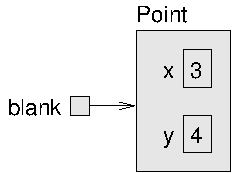
\includegraphics{figs/reference.pdf}
\caption{Memory diagram showing a variable that refers to a \java{Point} object.}
\label{fig.reference}
\end{center}
\end{figure}

As usual, the name of the variable \java{blank} appears outside the box, and its value appears inside the box.
In this case, the value is a reference, which is represented with an arrow.
The arrow points to the \java{Point} object, which contains two variables, \java{x} and \java{y}.


%\section{Attributes}

\index{attribute}
\index{dot notation}

Variables that belong to an object are called {\bf attributes}, but you might also see them referred to as ``fields'' in the documentation.
To access an attribute of an object, Java uses {\bf dot notation}.
For example:

\begin{code}
int x = blank.x;
\end{code}

The expression \java{blank.x} means ``go to the object \java{blank} refers to, and get the value of the attribute \java{x}.''
In this case, we assign that value to a local variable named \java{x}.

There is no conflict between the local variable named \java{x} and the attribute named \java{x}.
The purpose of dot notation is to identify {\em which} variable you are referring to unambiguously.

You can use dot notation as part of an expression.
For example:

\begin{code}
System.out.println(blank.x + ", " + blank.y);
int sum = blank.x * blank.x + blank.y * blank.y;
\end{code}

The first line displays \java{3, 4}.
The second line calculates the value \java{25}.


\section{Objects as parameters}

\index{parameter}
\index{object!as parameter}

You can pass objects as parameters in the usual way.
For example:

\begin{code}
public static void printPoint(Point p) {
    System.out.println("(" + p.x + ", " + p.y + ")");
}
\end{code}

This method takes a point as an argument and displays its attributes in parentheses.
If you invoke \java{printPoint(blank)}, it displays \java{(3, 4)}.

As another example, we can rewrite the \java{distance} method from Section~\ref{distance} so that it takes two \java{Point}s as parameters instead of four \java{double}s.

\begin{code}
public static double distance(Point p1, Point p2) {
    int dx = p2.x - p1.x;
    int dy = p2.y - p1.y;
    return Math.sqrt(dx * dx + dy * dy);
}
\end{code}

Passing objects as parameters makes the source code more readable and less error-prone, because related values are bundled together.

You actually don't need to write a \java{distance} method, because \java{Point} objects have one built-in already.
To compute the distance between two points, we invoke \java{distance} on one and pass the other as an argument.

\begin{code}
Point p1 = new Point(0, 0);
Point p2 = new Point(3, 4);
double dist = p1.distance(p2);  // dist is 5.0
\end{code}

It turns out you don't need the \java{printPoint} method either.
If you invoke \java{System.out.println(blank)} you get even more information:

\begin{stdout}
java.awt.Point[x=3,y=4]
\end{stdout}

\index{toString}

\java{Point} objects provide a method called \java{toString} that returns a string representation of a point.
When you call \java{println} with objects, it automatically calls \java{toString} and displays the result.
In this case, it shows the name of the type (\java{java.awt.Point}) and the names and values of the attributes.


\section{Objects as return types}

\index{Rectangle}
\index{class!Rectangle}

The \java{java.awt} package also provides a class named \java{Rectangle}.
To use it, you have to import it:

\begin{code}
import java.awt.Rectangle;
\end{code}

\java{Rectangle} objects are similar to points, but they have four attributes: \java{x}, \java{y}, \java{width}, and \java{height}.
The following example creates a \java{Rectangle} object and makes the variable \java{box} refer to it:

\begin{code}
Rectangle box = new Rectangle(0, 0, 100, 200);
\end{code}

Figure~\ref{fig.rectangle} shows the effect of this assignment.

\begin{figure}[!ht]
\begin{center}
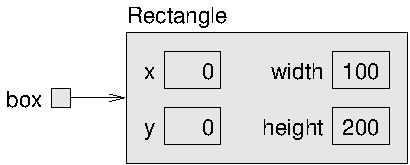
\includegraphics{figs/rectangle.pdf}
\caption{Memory diagram showing a \java{Rectangle} object.}
\label{fig.rectangle}
\end{center}
\end{figure}

If you run \java{System.out.println(box)}, you get:

\begin{stdout}
java.awt.Rectangle[x=0,y=0,width=100,height=200]
\end{stdout}

Again, \java{println} uses the \java{toString} method provided by \java{Rectangle}, which knows how to convert \java{Rectangle} objects into strings.

\index{return}
\index{statement!return}

You can write methods that return new objects.
For example, \java{findCenter} takes a \java{Rectangle} as an argument and returns a \java{Point} with the coordinates of the center of the rectangle:

\begin{code}
public static Point findCenter(Rectangle box) {
    int x = box.x + box.width / 2;
    int y = box.y + box.height / 2;
    return new Point(x, y);
}
\end{code}

The return type of this method is \java{Point}.
The last line creates a new \java{Point} object and returns a reference to it.

\index{coordinate}

You are probably used to Cartesian {\bf coordinates}, where $x$ and $y$ values can be positive or negative.
In contrast, Java uses a coordinate system where the origin is in the upper-left corner.
That way, $x$ and $y$ are always positive integers.
Figure~\ref{fig.coord} shows these coordinate systems side-by-side.

\begin{figure}[!ht]
\begin{center}
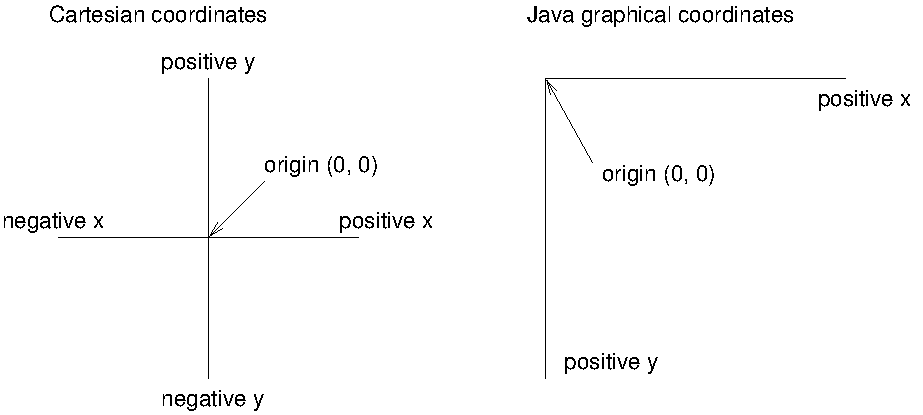
\includegraphics[width=5in]{figs/coordinates.pdf}
\caption{Diagram of the difference between Cartesian coordinates and Java graphical coordinates.}
\label{fig.coord}
\end{center}
\end{figure}

\index{pixel}

Graphical coordinates are measured in {\bf pixels}; each pixel corresponds to a dot on the screen.
You can learn more about Java 2D graphics in Appendix~\ref{graphics}.

The \java{Rectangle} we created using the arguments \java{(0, 0, 100, 200)} has its upper-left corner in the origin.
The center of this rectangle is \java{(50, 100)}, which is 50 pixels to the right and 100 pixels down from the origin.


\section{Rectangles are mutable}

\index{mutable}
\index{object!mutable}

You can change the contents of an object by making an assignment to one of its attributes.
For example, to ``move'' a rectangle without changing its size, you can modify the \java{x} and \java{y} values:

\begin{code}
Rectangle box = new Rectangle(0, 0, 100, 200);
box.x = box.x + 50;
box.y = box.y + 100;
\end{code}

The result is shown in Figure~\ref{fig.rectangle2}.

\begin{figure}[!ht]
\begin{center}
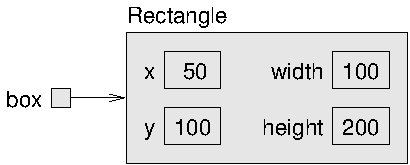
\includegraphics{figs/rectangle2.pdf}
\caption{Memory diagram showing updated attributes.}
\label{fig.rectangle2}
\end{center}
\end{figure}

\index{encapsulation}
\index{generalization}

We can encapsulate this code in a method and generalize it to move the rectangle by any amount:

\begin{code}
public static void moveRect(Rectangle box, int dx, int dy) {
    box.x = box.x + dx;
    box.y = box.y + dy;
}
\end{code}

The variables \java{dx} and \java{dy} indicate how far to move the rectangle in each direction.
Invoking this method has the effect of modifying the \java{Rectangle} that is passed as an argument.

\begin{code}
Rectangle box = new Rectangle(0, 0, 100, 200);
moveRect(box, 50, 100);  // now at (50, 100, 100, 200)
\end{code}

%The code displays \java{java.awt.Rectangle[x=50,y=100,width=100,height=200]}.

Modifying objects by passing them as arguments to methods can be useful.
But it can also make debugging more difficult, because it is not always clear which method invocations modify their arguments.

Java provides a number of methods that operate on \java{Point}s and \java{Rectangle}s.
For example, \java{translate} has the same effect as \java{moveRect}, but instead of passing the rectangle as an argument, you use dot notation:

\begin{code}
box.translate(50, 100);
\end{code}

This line invokes the \java{translate} method for the object that \java{box} refers to.
As a result, the \java{box} object is updated directly.

\index{object-oriented}

This example is a further illustration of {\bf object-oriented} programming.
Rather than write methods like \java{moveRect} that modify one or more parameters, we apply methods to objects themselves using dot notation.


\section{Aliasing revisited}
\label{aliasing}

\index{reference}

Remember that when you assign an object to a variable, you are assigning a {\em reference} to an object.
It is possible to have multiple variables that refer to the same object.
The memory diagram in Figure~\ref{fig.aliasing} shows the result.

\begin{code}
Rectangle box1 = new Rectangle(0, 0, 100, 200);
Rectangle box2 = box1;
\end{code}

\begin{figure}[!ht]
\begin{center}
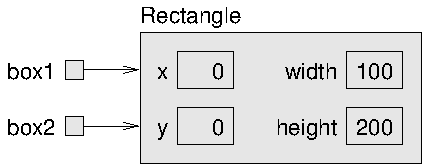
\includegraphics{figs/aliasing.pdf}
\caption{Memory diagram showing two variables that refer to the same \java{Rectangle} object.}
\label{fig.aliasing}
\end{center}
\end{figure}

\index{aliasing}

%Notice how \java{box1} and \java{box2} are aliases for the same object, so any changes that affect one variable also affect the other.

The following example adds 50 to all four sides of the rectangle.
It moves the corner up and to the left by 50, and it increases the height and width by 100:

\begin{code}
System.out.println(box2.width);   // box2.width is 100
box1.grow(50, 50);                // grow box1 (alias)
System.out.println(box2.width);   // box2.width is 200
\end{code}

The first line displays {\tt 100}, which is the width of the \java{Rectangle} referred to by \java{box2}.
The second line invokes the \java{grow} method on \java{box1}, which stretches the \java{Rectangle} horizontally and vertically.
The effect is shown in Figure~\ref{fig.aliasing2}.

\begin{figure}[!ht]
\begin{center}
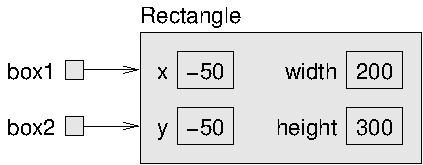
\includegraphics{figs/aliasing2.pdf}
\caption{Memory diagram showing the effect of invoking \java{grow}.}
\label{fig.aliasing2}
\end{center}
\end{figure}

When we make a change using \java{box1}, we see the change using \java{box2}.
Thus, the value displayed by the third line is {\tt 200}, the width of the expanded rectangle.
%(As an aside, it is perfectly legal for the coordinates of a \java{Rectangle} %to be negative.)

%As you can tell from this simple example, code that involves aliasing can get confusing fast, and it can be difficult to debug.
%In general, aliasing should be avoided or used with care.


\section{Java library source}
\label{src.zip}

\index{library}
\index{source code}

Throughout the book, you have used classes from the Java library including \java{System}, \java{String}, \java{Scanner}, \java{Math}, \java{Random}, and others.
You may not have realized that these classes are written in Java.
In fact, you can take a look at the source code to see how they work.

\index{src.zip}

The Java library contains thousands of files, many of which are thousands of lines of code.
That's more than one person could read and understand fully, so don't be intimidated!

Because it's so large, the library source code is stored in a ZIP archive named \java{src.zip}.
Take a few minutes to locate this file on your computer.
In the paths below, you'll need to replace ``\java{...}'' with the version number.

\begin{itemize}
\item On Linux, it's likely under: \verb"/usr/lib/jvm/openjdk-.../"
\\ If not, then install the {\tt openjdk-...-source} package.
\item On MacOS, it's likely under: \\ \verb"/Library/Java/JavaVirtualMachines/jdk.../Contents/Home/"
\item On Windows, it's likely under: \verb"C:\Program Files\Java\jdk...\"
\end{itemize}

When you open (or unzip) the file, you will see folders that correspond to Java packages.
For example, open the {\tt java} folder, and then open the {\tt awt} folder.
You should now see {\tt Point.java} and {\tt Rectangle.java}, along with the other classes in the \java{java.awt} package.

Open {\tt Point.java} in your editor and skim through the file.
It uses language features we haven't yet discussed, so you probably won't understand every single line.
But you can get a sense of what professional Java source code looks like by browsing through the library.

\index{documentation}
\index{HTML}
\index{Javadoc}

Notice how much of {\tt Point.java} is documentation (see Appendix~\ref{javadoc}).
Each method is thoroughly commented, including \java{@param}, \java{@return}, and other tags.
Javadoc reads these comments and generates documentation in HTML.
You can see the results by reading the documentation for the \java{Point} class, which you can find by doing a web search for ``Java Point''.

Now take a look at the \java{Rectangle} class's \java{grow} and \java{translate} methods.
There is more to them than you may have realized, but that doesn't limit your ability to use these methods in a program.
Object-oriented programming makes it possible to hide messy details so that you can more easily use and understand code that other people wrote.

%By looking at the source code for \java{Point}, \java{Rectangle}, and other classes, we hope you will learn two things.
%1) Objects encapsulate data and provide methods to access and modify the data directly.


\section{Class diagrams}
\label{UML}

To summarize what we've learned so far, \java{Point} and \java{Rectangle} objects each have their own attributes and methods.
Attributes are an object's {\em data}, and methods are an object's {\em code}.
An object's {\em class} defines which attributes and methods it will have.

\index{UML}

In practice, it's more convenient to look at high-level pictures than to examine the details of source code.
{\bf Unified Modeling Language} (UML) defines a standard way to summarize the design of a class.

\begin{figure}[!ht]
\begin{center}
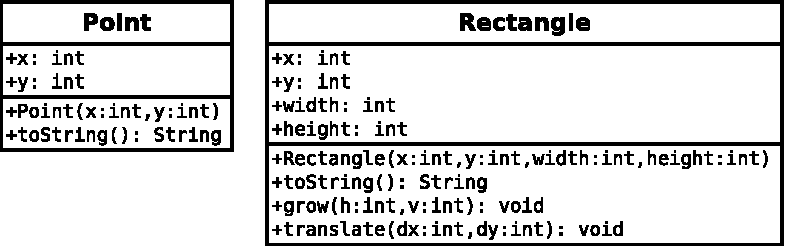
\includegraphics{figs/point-rect.pdf}
\caption{UML class diagrams for \java{Point} and \java{Rectangle}.}
\label{fig.umlPoint}
\end{center}
\end{figure}

\index{class diagram}
\index{diagram!class}

As shown in Figure~\ref{fig.umlPoint}, a {\bf class diagram} is divided into two sections.
The top half lists the attributes, and the bottom half lists the methods.

\index{private}
\index{variable!private}

UML uses a language-independent format, so rather than showing \java{int x}, the diagram uses {\tt x:~int}.
The plus sign (\java{+}) means that the attributes and methods are \java{public}.
%In the case of these two classes, everything is \java{public}.
We'll get to \java{private} attributes (\java{-}) in the next chapter.

In contrast to memory diagrams, which visualize objects (and variables) at run-time, a class diagram visualizes the source code at compile-time.

Both \java{Point} and \java{Rectangle} have additional methods; we are only showing the ones introduced in this chapter.
See the documentation for these classes to learn more about what they can do.


\section{Garbage collection}

In Section~\ref{aliasing}, we saw what happens when more than one variable refers to the same object.
What happens when {\em no} variables refer to an object?

\begin{code}
Point blank = new Point(3, 4);
blank = null;
\end{code}

The first line creates a new \java{Point} object and makes \java{blank} refer to it.
The second line changes \java{blank} so that instead of referring to the object, it refers to nothing.
As shown in Figure~\ref{fig.reference3}, there is no longer an arrow between them.

\begin{figure}[!ht]
\begin{center}
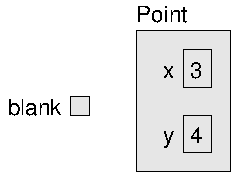
\includegraphics{figs/reference3.pdf}
\caption{Memory diagram showing the effect of setting a variable to \java{null}.}
\label{fig.reference3}
\end{center}
\end{figure}

If there are no references to an object, there is no way to access its attributes or invoke a method on it.
From the program's point of view, it ceases to exist.
However, it's still present in the computer's memory, taking up space.

\index{garbage collection}

As your program runs, the system automatically looks for stranded objects and deletes them; then the space can be reused for new objects.
This process is called {\bf garbage collection}.
%You can manually run the garbage collector by invoking \java{System.gc()} method.

You don't have to do anything to make garbage collection happen, and in general don't have to be aware of it.
But in high-performance applications, you may notice a slight delay every now and then when Java reclaims space from discarded objects.


\section{Mutable vs immutable}

\index{mutable}
\index{immutable}

\java{Point}s and \java{Rectangle}s are {\bf mutable} objects, because their attributes can be modified.
You can modify their attributes directly, like \java{box.x = 15}, or you can invoke methods that modify their attributes, like \java{box.translate(15, 0)}.

In contrast, immutable objects like \java{String}s and \java{Integer}s cannot be modified.
They do not give \java{public} access to their attributes, and they do not provide methods that change their attributes.

Immutable objects have a number of advantages that help improve the performance and reliability of programs.
For example, two strings that contain the same contents can be stored in memory only once.
The Java compiler automatically detects this situation:

\index{Surprise.java}

\begin{trinket}[265]{Surprise.java}
public class Surprise {
    public static void main(String[] args) {
        String s1 = "Hi, Mom!";
        String s2 = "Hi, " + "Mom!";
        if (s1 == s2) {  // true!
            System.out.println("s1 and s2 are the same");
        }
    }
}
\end{trinket}

In this example, \java{s1} and \java{s2} represent the {\em same} string, even though they are created differently.
Because strings are immutable, the compiler decides to reuse a single object for both \java{s1} and \java{s2}.
As a result, \java{s1 == s2}, even though it appears they should be different objects.

Since neither variable can change the string itself, both \java{s1} and \java{s2} will be \java{"Hi, Mom!"} until they are reassigned.
You can pass strings (and other immutable objects) to methods without worrying about their contents changing as a ``side-effect'' of the method.

\index{efficiency}

On the other hand, mutable objects have their own advantages.
It's more efficient to move a rectangle by simply changing its coordinates than to create a brand new \java{Rectangle} each time.
And as we'll see later on, it's easier to implement objects that allow their attributes to be changed.

Strings are particularly inefficient when you need to concatenate them multiple times.
Consider the following program that inputs ten lines from \java{System.in} and concatenates them into a single \java{String}.

\index{Append.java}

\begin{trinket}[325]{Append.java}
import java.util.Scanner;
public class Append {
    public static void main(String[] args) {
        Scanner in = new Scanner(System.in);
        System.out.println("Enter 10 lines:");
        String text = "";
        for (int i = 0; i < 10; i++) {
            String line = in.nextLine();        // new string
            text = text + line + '\n';    // two more strings
        }
        System.out.print("You entered:\n" + text);
    }
}
\end{trinket}

Each time that \java{in.nextLine()} is invoked, it returns a new string.
The next line of code performs \java{text + line}, which creates another string, and then appends the newline character, which creates yet another string.

As a result, the \java{for} loop creates 30 \java{String} objects!
The variable \java{text} references only the most recent \java{String} object.
Garbage collection will delete the other strings, but that's a lot of garbage for a seemly simple program.

The Java library provides the class \java{StringBuilder} for this situation.
It's part of the \java{java.lang} package, so you don't need to import it.
Because \java{StringBuilder} objects are mutable, they can implement concatenation much more efficiently.

All we need to change is the \java{text} variable and the body of the \java{for} loop:

\begin{code}
StringBuilder text = new StringBuilder();
for (int i = 0; i < 10; i++) {
    String line = in.nextLine();
    text.append(line);
    text.append('\n');
}
\end{code}

\java{StringBuilder} provides a number of \java{append} and \java{insert} methods that work with strings efficiently.
It also allows you to \java{delete} portions of a string.


\section{Vocabulary}

\begin{description}

\term{attribute}
One of the named data items that make up an object.
%Each object has its own copy of the attributes for its class.

\term{dot notation}
Use of the dot operator (\java{.}) to access an object's attributes or methods.

\term{coordinate}
A value that specifies a location in a 2D graphical window.

\term{pixel}
The unit in which coordinates are measured.

\term{object-oriented}
A way of organizing code and data into objects, rather than independent methods.

\term{UML}
Unified Modeling Language, a standard way to draw diagrams for software engineering.

\term{class diagram}
An illustration of the attributes and methods for a class.

\term{garbage collection}
The process of finding objects that have no references and reclaiming their storage space.

\term{mutable}
An object that can be modified at any time.
Points and rectangles are mutable by design.

\end{description}


\section{Exercises}

The code for this chapter is in the {\tt ch10} directory of {\tt ThinkJavaCode2}.
See page~\pageref{code} for instructions on how to download the repository.
Before you start the exercises, we recommend that you compile and run the examples.

At this point you know enough to read Appendix~\ref{graphics}, which is about simple 2D graphics and animations.
During the next few chapters, you should take a detour to read this appendix and work through the exercises.


\begin{exercise}  %%V6 Ex10.1

The point of this exercise is to make sure you understand the mechanism for passing objects as parameters.

\begin{enumerate}

\item For the following program, draw a stack diagram showing the local variables and parameters of \java{main} and \java{riddle} just before \java{riddle} returns.
Use arrows to show which objects each variable references.

\item What is the output of the program?

\item Is the \java{blank} object mutable or immutable?
How can you tell?

\end{enumerate}

\begin{code}
public static int riddle(int x, Point p) {
    x = x + 7;
    return x + p.x + p.y;
}
\end{code}

\begin{code}
public static void main(String[] args) {
    int x = 5;
    Point blank = new Point(1, 2);

    System.out.println(riddle(x, blank));
    System.out.println(x);
    System.out.println(blank.x);
    System.out.println(blank.y);
}
\end{code}

\end{exercise}


\begin{exercise}  %%V6 Ex10.2

The point of this exercise is to make sure you understand the mechanism for returning new objects from methods.
The following code uses \java{findCenter} and \java{distance} as defined in this chapter.

\begin{enumerate}

\item Draw a stack diagram showing the state of the program just before \java{findCenter} returns.
Include all variables and parameters, and show the objects those variables refer to.

\item Draw a stack diagram showing the state of the program just before \java{distance} returns.
Show all variables, parameters, and objects.

\item What is the output of this program?
(Can you tell without running it?)

\end{enumerate}

\begin{code}
public static void main(String[] args) {
    Point blank = new Point(5, 8);

    Rectangle rect = new Rectangle(0, 2, 4, 4);
    Point center = findCenter(rect);

    double dist = distance(center, blank);
    System.out.println(dist);
}
\end{code}

\end{exercise}


\begin{exercise}  %%V6 Ex10.3

This exercise is about aliasing.
Recall that aliases are two variables that refer to the same object.
The following code uses \java{findCenter} and \java{printPoint} as defined in this chapter.

\begin{enumerate}

\item Draw a diagram that shows the state of the program just before the end of \java{main}.
Include all local variables and the objects they refer to.

\item What is the output of the program?

\item At the end of \java{main}, are \java{p1} and \java{p2} aliased?
Why or why not?

\end{enumerate}

\begin{code}
public static void main(String[] args) {
    Rectangle box1 = new Rectangle(2, 4, 7, 9);
    Point p1 = findCenter(box1);
    printPoint(p1);

    box1.grow(1, 1);
    Point p2 = findCenter(box1);
    printPoint(p2);
}
\end{code}

\end{exercise}
}
% Modified on 1/13/05.
\newdimen\snellbaselineskip
\newdimen\snellskip
\snellskip=1.5ex
\snellbaselineskip=\baselineskip
\def\srule{\omit\kern.5em\vrule\kern-.5em}
\newbox\bigstrutbox
\setbox\bigstrutbox=\hbox{\vrule height14.5pt depth9.5pt width0pt}
\def\bigstrut{\relax\ifmmode\copy\bigstrutbox\else\unhcopy\bigstrutbox\fi}
\def\middlehrule#1#2{\noalign{\kern-\snellbaselineskip\kern\snellskip}
&\multispan#1\strut\hrulefill
&\omit\hbox to.5em{\hrulefill}\vrule 
height \snellskip\kern-.5em&\multispan#2\hrulefill\cr}

\makeatletter
\def\bordermatrix#1{\begingroup \m@th
  \@tempdima 8.75\p@
  \setbox\z@\vbox{%
    \def\cr{\crcr\noalign{\kern2\p@\global\let\cr\endline}}%
    \ialign{$##$\hfil\kern2\p@\kern\@tempdima&\thinspace\hfil$##$\hfil
      &&\quad\hfil$##$\hfil\crcr
      \omit\strut\hfil\crcr\noalign{\kern-\snellbaselineskip}%
      #1\crcr\omit\strut\cr}}%
  \setbox\tw@\vbox{\unvcopy\z@\global\setbox\@ne\lastbox}%
  \setbox\tw@\hbox{\unhbox\@ne\unskip\global\setbox\@ne\lastbox}%
  \setbox\tw@\hbox{$\kern\wd\@ne\kern-\@tempdima\left(\kern-\wd\@ne
    \global\setbox\@ne\vbox{\box\@ne\kern2\p@}%
    \vcenter{\kern-\ht\@ne\unvbox\z@\kern-\snellbaselineskip}\,\right)$}%
  \null\;\vbox{\kern\ht\@ne\box\tw@}\endgroup}

\makeatother



%\setcounter{chapter}{9}

\chapter{Markov Chains}\label{chp 11}  

\section{Introduction}\label{sec 11.1}

\par
Most of our study of probability has dealt with independent trials processes. 
These processes are the basis of classical probability theory and much of
statistics.  We have discussed two of the principal theorems for these
processes: the Law of Large Numbers and the Central Limit Theorem.
\par
We have seen that when a sequence of chance experiments forms an independent
trials process, the possible outcomes for each experiment are the same and
occur with the same probability.  Further, knowledge of the outcomes of the
previous experiments does not influence our predictions for the outcomes of the
next experiment.  The distribution for the outcomes of a single experiment is
sufficient to construct a tree and a tree measure for a sequence of $n$
experiments, and we can answer any probability question about these 
experiments by using this tree measure.
\par
Modern probability theory studies chance processes for which the knowledge of
previous outcomes influences predictions for future experiments.  In principle,
when we observe a sequence of chance experiments, all of the past outcomes
could influence our predictions for the next experiment.  For example, this
should be the case in predicting a student's grades on a sequence of exams in a
course.  But to allow this much generality would make it very difficult to
prove general results.
\par
In 1907, A.~A. Markov began the study of an important new type of chance
process.  In this process, the outcome of a given experiment can affect the
outcome of the next experiment.  This type of process is called a Markov
chain.
\subsection*{Specifying a Markov Chain}\index{Markov chain}
We  describe a Markov chain as follows:  We have a set of \emx {states,} $S =
\{s_1,s_2,\ldots,s_r\}$.\index{state!of a Markov chain}  The process starts in
one of 
these states and moves successively from one state to another.  Each
move is called a  \emx {step.}  If the chain is currently in state $s_i$, then
it
moves to state $s_j$ at the next step with a probability denoted by $p_{ij}$,
and this
probability does not depend upon which states the chain was in before the
current state.
\par
The probabilities~$p_{ij}$ are called \emx {transition
probabilities.}\index{transition
probability}\index{probability!transition}  The process can remain in the state
it is in,
and this occurs with probability~$p_{ii}$.  An initial probability
distribution, defined
on~$S$, specifies the starting state.  Usually this is done by specifying a
particular
state as the starting state.

R.~A. Howard\footnote{R.~A. Howard, \emx {Dynamic Probabilistic Systems,}
vol.~1
(New York: John Wiley and Sons, 1971).}\index{HOWARD, R. A.} provides us with a
picturesque
description of a Markov chain as a frog jumping on a set of lily pads. 
The frog starts on one of the pads and then jumps from lily pad to lily
pad with the appropriate transition probabilities.



\begin{example}\label{exam 11.1.1}
According to Kemeny, Snell, and Thompson,\footnote{J.~G. Kemeny, J.~L. Snell,
G.~L. Thompson, \emx {Introduction to Finite Mathematics,} 3rd ed.\ (Englewood
Cliffs, NJ: Prentice-Hall, 1974).}\index{KEMENY, J. G.}\index{SNELL, J.
L.}\index{THOMPSON, G. L.} the Land of Oz\index{Oz, Land of} is blessed by many
things, but
not by good weather.  They never have two nice days in a row.  If they have a
nice day,
they are just as likely to have snow as rain the next day.  If they have snow
or rain, they
have an even chance of having the same the next day.  If there is change from
snow or
rain, only half of the time is this a change to a nice day.  With this
information we form a
Markov chain as follows.  We take as states the kinds of weather R, N, and S. 
From the above information we determine the transition probabilities.  These are most
conveniently represented
in a square array as
$$
\mat {P} = \bordermatrix{
        & \mbox {R} & \mbox {N} & \mbox {S} \cr
\mbox {R} &     1/2 &     1/4 &     1/4 \cr
\mbox {N} &     1/2 &       0 &     1/2 \cr
\mbox {S} &     1/4 &     1/4 &     1/2}\ .
$$
\end{example}

\subsection*{Transition Matrix}
The entries in the first row of the matrix $\mat {P}$ in Example~\ref{exam
11.1.1}
represent  the probabilities for the various kinds of weather following a rainy
day.
Similarly, the entries in the second and third rows represent the probabilities
for
the various kinds of weather following nice and snowy days, respectively.
Such a square array is called the \emx {matrix of transition
probabilities}, or the  \emx {transition matrix}.\index{transition matrix}
\par
We consider the question of determining the probability that, given the chain
is in
state $i$ today, it will be in state $j$ two days from now.  We denote this
probability by $p_{ij}^{(2)}$.  In Example~\ref{exam 11.1.1}, we see that if it
is
rainy today then the event that it is snowy two days from now is the disjoint
union
of the following three events: 1) it is rainy tomorrow and snowy two days from
now,
2) it is nice tomorrow and snowy two days from now, and 3) it is snowy tomorrow
and
snowy two days from now.  The probability of the first of these events is the
product
of the conditional probability that it is rainy tomorrow, given that it is
rainy today,
and the conditional probability that it is snowy two days from now, given that
it is
rainy tomorrow.  Using the transition matrix $\mat{P}$, we can write this
product as
$p_{11}p_{13}$.  The other two events also have probabilities that can be
written as products
of entries of $\mat{P}$.  Thus, we have
$$p_{13}^{(2)} = p_{11}p_{13} + p_{12}p_{23} + p_{13}p_{33}\ .$$
This equation should remind the reader of a dot product of two vectors; we are
dotting the first
row of $ \mat {P}$ with the third column of $ \mat {P}$.  This is just what is
done in
obtaining the $1,3$-entry of the product of $ \mat {P}$ with itself.  
In general, if a Markov chain has $r$ states, then
$$p_{ij}^{(2)} = \sum_{k = 1}^r p_{ik}p_{kj}\ .$$
The following general theorem is easy to prove by using the above observation
and
induction.
\begin{theorem}\label{thm 11.1.1}
Let $ \mat {P}$ be the transition matrix of a Markov chain.  The $ij$th
entry~$p_{ij}^{(n)}$ of the matrix~$ \mat {P}^n$ gives the
probability that the Markov chain, starting in state~$s_i$, will be in
state~$s_j$ after $n$ steps.
\proof
The proof of this theorem is left as an exercise (Exercise~\ref{exer 11.1.18}).
\end{theorem}

\begin{example}\label{exam 11.1.1.5} (Example~\ref{exam 11.1.1} continued)
Consider again the weather in the Land of Oz.  We know that the powers of the
transition matrix give us interesting information about the process as it
evolves.  We shall be particularly interested in the state of the chain after a
large number of steps.  The program {\bf MatrixPowers}\index{MatrixPowers (program)} computes
the powers of~$\mat{P}$.
\par
We have run the program {\bf MatrixPowers} for the Land of Oz example
to compute the successive powers of~$\mat{P}$ from 1~to~6. The results are
shown 
in Table~\ref{table 11.1}.  We note that after six days our weather predictions
are, 
to three-decimal-place accuracy, independent of today's weather.  The
probabilities for the three 
types of weather, R, N, and S, are .4, .2, and .4 no matter where the chain
started.  This is an
example of a type of Markov chain called a \emx {regular} Markov chain.  For
this type of chain,
it is true that long-range predictions are independent of the starting state. 
Not all chains are
regular, but this is an important class of chains that we shall study in detail
later.
\begin{table}
\centering
$$
\mat{P}^1  = \bordermatrix{
            &\mbox{Rain}&\mbox{Nice}&\mbox{Snow} \cr
\mbox{Rain} & .500      & .250      & .250 \cr
\mbox{Nice} & .500      & .000      & .500 \cr
\mbox{Snow} & .250      & .250      & .500 \cr}
$$
$$  
\mat {P}^2  = \bordermatrix{
            &\mbox{Rain}&\mbox{Nice}&\mbox{Snow} \cr
\mbox{Rain} & .438     & .188       & .375 \cr
\mbox{Nice} & .375     & .250       & .375 \cr
\mbox{Snow} & .375     & .188       & .438 \cr}
$$
$$
\mat {P}^3  = \bordermatrix{
            &\mbox{ Rain}&\mbox{Nice} &\mbox{Snow} \cr
\mbox{Rain} & .406       & .203       & .391 \cr
\mbox{Nice} & .406       & .188       & .406 \cr
\mbox{Snow} & .391       & .203       & .406 \cr}
$$
$$  
\mat {P}^4  = \bordermatrix{
            &\mbox{Rain}&\mbox{Nice}&\mbox{Snow} \cr
\mbox{Rain} & .402      & .199      & .398 \cr
\mbox{Nice} & .398      & .203      & .398 \cr
\mbox{Snow} & .398      & .199      & .402 \cr}
$$
$$
\mat {P}^5  = \bordermatrix{
           &\mbox{Rain}&\mbox{Nice}&\mbox{Snow} \cr
\mbox{Rain} & .400     & .200     & .399 \cr
\mbox{Nice} & .400     & .199     & .400 \cr
\mbox{Snow} & .399     & .200     & .400 \cr}
$$
$$  
\mat {P}^6  = \bordermatrix{
           &\mbox{Rain}&\mbox{Nice}&\mbox{Snow} \cr
\mbox{Rain} & .400     & .200     & .400 \cr
\mbox{Nice} & .400     & .200     & .400 \cr
\mbox{Snow} & .400     & .200     & .400 \cr}
$$
\caption{Powers of the Land of Oz transition matrix.}
\label{table 11.1}
\end{table}
\end{example}

We now consider the long-term behavior of a Markov chain when it starts in a
state chosen by a probability distribution
on the set of states, which we will call a \emx {probability
vector}.\index{probability!vector}  A probability vector with $r$ components is
a row
vector whose entries are non-negative and sum to 1.  If $\mat
{u}$ is a probability vector which represents the initial state of a Markov
chain, then we
think of the $i$th component of $\mat {u}$ as representing the probability that
the
chain starts in state $s_i$.
\par
With this interpretation of random starting states, it is easy to prove the
following theorem.
\begin{theorem}\label{thm 11.1.2}
Let $\mat{P}$ be the transition matrix of a Markov chain, and let $\mat {u}$ be
the
probability vector which represents the starting distribution.  Then the
probability
that the chain is in state $s_i$ after $n$ steps is the $i$th entry in the
vector
$$ \mat{u}^{(n)} = \mat{u}{\mat{P}^n}\ .$$
\proof
The proof of this theorem is left as an exercise (Exercise~\ref{exer 11.1.19}).
\end{theorem}

We note that if we want to examine the behavior of the chain under the
assumption
that it starts in a certain state $s_i$, we simply choose $\mat {u}$ to be the
probability vector with $i$th entry equal to 1 and all other entries equal to
0.

\begin{example}\label{exam 11.1.1.6} In the Land of Oz example
(Example~\ref{exam 11.1.1}) let the
initial probability vector $\mat {u}$ equal $(1/3, 1/3, 1/3)$.  Then we can
calculate
the distribution of the states after three days using Theorem~\ref{thm
11.1.2} and our previous calculation of ${\mat {P}^3}$.  We obtain
\begin{eqnarray*}
{\mat {u}}^{(3)} = {\mat {u}}{\mat {P}^3} &=& \pmatrix{ 1/3,& 1/3,& 1/3}
\pmatrix{ .406 & .203 &
.391 \cr   .406 & .188 & .406 \cr .391 & .203 & .406 } \cr
&& \cr
&=& \pmatrix{ .401,& .198,& .401} \ .
\end{eqnarray*}
\end{example}

\subsection*{Examples}
The following examples of Markov chains will be used throughout the chapter for
exercises.

\begin{example}\label{exam 11.1.2}
The President of the United States tells person~A his or her intention to run
or 
not to run in the next election.  Then A relays the news to~B, who in turn
relays 
the message to~C, and so forth, always to some new person.  We assume that
there is
a probability~$a$ that a person will change the answer from yes to no when
transmitting it to the next person and a probability~$b$ that he or she will
change it
from no to yes.  We choose as states the message, either yes or no.  The
transition matrix is then
$$
\mat{P} = \bordermatrix{
           & \mbox{yes} & \mbox{no} \cr
\mbox{yes} &      1 - a &         a \cr
\mbox{no}  &          b &     1 - b}\ .
$$
The initial state represents the President's choice.
\end{example}

\begin{example}\label{exam 11.1.3}
Each time a certain horse runs in a three-horse race, he has probability~1/2 of
winning, 1/4 of coming in second, and 1/4 of coming in third, independent of
the
outcome of any previous race.  We have an independent trials process, but it
can also
be considered from the point of view of Markov chain theory.  The transition
matrix
is
$$
\mat{P} = \bordermatrix{
        & \mbox{W} & \mbox{P} & \mbox{S} \cr
\mbox{W} &      .5 &      .25 &      .25 \cr
\mbox{P} &      .5 &      .25 &      .25 \cr
\mbox{S} &      .5 &      .25 &      .25}\ .
$$
\end{example}
\vskip -3pt
\begin{example}\label{exam 11.1.4}
In the Dark Ages, Harvard, Dartmouth, and Yale admitted only male students. 
Assume that, at that time, 80~percent of the sons of Harvard men went to
Harvard
and the rest went to Yale, 40~percent of the sons of Yale men went to Yale, and
the rest split evenly between Harvard and Dartmouth; and of the sons of
Dartmouth men, 70~percent went to Dartmouth, 20~percent to Harvard, and
10~percent to Yale.  We form a Markov chain with transition matrix
$$
\mat{P} = \bordermatrix{
        & \mbox{H} & \mbox{Y} & \mbox{D} \cr
\mbox{H} &      .8 &      .2 &       0 \cr
\mbox{Y} &      .3 &      .4 &      .3 \cr 
\mbox{D} &      .2 &      .1 &      .7}\ .
$$
\end{example}
\vskip -3pt
\begin{example}\label{exam 11.1.5}
Modify Example~\ref{exam 11.1.4} by assuming that the son of a Harvard man
always went
to Harvard.  The transition matrix is now
$$
\mat{P} = \bordermatrix{
        & \mbox{H} & \mbox{Y} & \mbox{D} \cr
\mbox{H} &       1 &       0 &       0 \cr
\mbox{Y} &      .3 &      .4 &      .3 \cr
\mbox{D} &      .2 &      .1 &      .7}\ .
$$
\end{example}
\vskip -3pt
\begin{example}\label{exam 11.1.6}\index{Ehrenfest model}
\index{gas diffusion!Ehrenfest model of}
(Ehrenfest Model) The following is a special case of a model, called the
Ehrenfest
model,\footnote{P. and T. Ehrenfest, ``\"{U}ber zwei bekannte Einw\"{a}nde
gegen das
Boltzmannsche  H-Theorem," \emx {Physikalishce Zeitschrift,} vol.~8 (1907),
pp.~311-314.}\index{EHRENFEST, P.}
\index{EHRENFEST, T}
that has been used to explain diffusion of gases.  The general model will be
discussed in detail in Section~\ref{sec 11.5}.  We have two urns that, between
them,
contain four balls.  At each step, one of the four balls is chosen at random
and
moved from the urn that it is in into the other urn.  We choose, as states, the
number of balls in the first urn.  The transition matrix is then
$$
 \mat {P} = \bordermatrix{
  &  0  &  1  &  2  &  3  &  4  \cr
0 &  0  &  1  &  0  &  0  &  0  \cr
1 & 1/4 &  0  & 3/4 &  0  &  0  \cr
2 &  0  & 1/2 &  0  & 1/2 &  0  \cr
3 &  0  &  0  & 3/4 &  0  & 1/4 \cr
4 &  0  &  0  &  0  &  1  &  0 \cr}\ . 
$$
\end{example}

\begin{example}\label{exam 11.1.7}\index{genes}
(Gene Model) The simplest type of inheritance of traits in animals occurs when
a trait is
governed by a pair of genes, each of which may be of two types, say G~and~g. 
An individual may have a GG combination or Gg (which is genetically the same as
gG) or gg.  Very often the GG and Gg types are indistinguishable in appearance,
and then we say that the G~gene dominates the g~gene.  An individual is called
 \emx {dominant} if he or she has GG~genes, \emx {recessive} if he or she has
gg, and \emx {hybrid} with a Gg mixture.
\par
In the mating of two animals, the offspring inherits one gene of the pair from
each parent, and the basic assumption of genetics is that these genes are
selected at random, independently of each other.  This assumption determines
the probability of occurrence of each type of offspring.  The offspring of two
purely dominant parents must be dominant, of two recessive parents must be
recessive, and of one dominant and one recessive parent must be hybrid.
\par
In the mating of a dominant and a hybrid animal, each offspring must get a
G~gene from the former and has an equal chance of getting G~or~g from the
latter.  Hence there is an equal probability for getting a dominant or a hybrid
offspring.  Again, in the mating of a recessive and a hybrid, there is an even
chance for getting either a recessive or a hybrid.  In the mating of two
hybrids, the offspring has an equal chance of getting G~or~g from each parent. 
Hence the probabilities are 1/4 for GG, 1/2 for Gg, and 1/4 for gg.
\par
Consider a process of continued matings.  We start with an individual of
known genetic character and mate it with a hybrid.  We assume that there is at
least
one offspring.  An offspring is chosen at random and is mated with a hybrid and
this process
repeated through a number of generations.  The genetic type of the chosen
offspring in
successive generations can be represented by a Markov chain.  The states are
dominant, hybrid, and recessive, and indicated by GG, Gg, and gg respectively.
\par
The transition probabilities are
$$
\mat{P} = \bordermatrix{
          &\mbox{GG} & \mbox{Gg} & \mbox{gg} \cr
\mbox{GG} &  .5      & .5        &   0       \cr
\mbox{Gg} & .25      & .5        & .25       \cr
\mbox{gg} &   0      & .5        &  .5       }\ . 
$$
\end{example}

\begin{example}\label{exam 11.1.8}
Modify Example~\ref{exam 11.1.7} as follows:  Instead of mating the oldest
offspring with a hybrid, we mate it with a dominant individual.  The transition
matrix
is
$$
\mat{P} = \bordermatrix{
   & \mbox{GG} & \mbox{Gg} &\mbox{gg} \cr
\mbox{GG} &  1 &  0 &  0 \cr
\mbox{Gg} & .5 & .5 &  0 \cr
\mbox{gg} &  0 &  1 &  0}\ .
$$
\end{example}

\begin{example}\label{exam 11.1.9}
We start with two animals of opposite sex, mate them, select two of their
offspring of opposite sex, and mate those, and so forth.  To simplify the
example, we will assume that the trait under consideration is independent of
sex.
\par
Here a state is determined by a pair of animals.  Hence, the states of our
process will be: $s_1 = (\mbox{GG},\mbox{GG})$, $s_2 = (\mbox{GG},\mbox{Gg})$,
$s_3 = (\mbox{GG},\mbox{gg})$, $s_4 = (\mbox{Gg},\mbox{Gg})$, $s_5 =
(\mbox{Gg},\mbox{gg})$, and $s_6 = (\mbox{gg},\mbox{gg})$.
\par
We illustrate the calculation of transition probabilities in terms of the
state~$s_2$.  When the process is in this state, one parent has GG~genes, the
other Gg.  Hence, the probability of a dominant offspring is~1/2.  Then the
probability of transition to~$s_1$ (selection of two dominants) is~1/4,
transition to~$s_2$ is~1/2, and to~$s_4$ is~1/4.  The other states are treated
the same way.  The transition matrix of this chain is:  
\par

$$
{\mat{P}^1} = \bordermatrix{            
&\mbox{GG,GG}&\mbox{GG,Gg}&\mbox{GG,gg}&\mbox{Gg,Gg}&\mbox{Gg,gg}&\mbox{gg,gg}\cr
\mbox{GG,GG} & 1.000 & .000 &  .000 &  .000 &  .000 &  .000\cr
\mbox{GG,Gg} &  .250 & .500 &  .000 &  .250 &  .000 &  .000\cr
\mbox{GG,gg} &  .000 & .000 &  .000 & 1.000 &  .000 &  .000\cr
\mbox{Gg,Gg} &  .062 & .250 &  .125 &  .250 &  .250 &  .062\cr
\mbox{Gg,gg} &  .000 & .000 &  .000 &  .250 &  .500 &  .250\cr
\mbox{gg,gg} &  .000 & .000 &  .000 &  .000 &  .000 &  1.000}\ .
$$
 
\end{example}

\begin{example} \label{exam 11.1.10}\index{stepping stones}
(Stepping Stone Model)  Our final example is another example that has been used
in the
study of genetics.  It is called the \emx {stepping stone} model.\footnote{S.
Sawyer, ``Results for The Stepping Stone Model for Migration in Population
Genetics," \emx {Annals of Probability,} vol.~4 (1979),
pp.~699--728.}\index{SAWYER, S.}  In this
model we have an $n$-by-$n$ array of squares, and each square is initially any
one of $k$ different colors.  For each step, a square is chosen at random. 
This
square then chooses one of its eight neighbors at random and assumes the color
of that neighbor.  To avoid boundary problems, we assume that if a square $S$
is on the
left-hand boundary, say, but not at a corner, it is adjacent to the square $T$
on the
right-hand boundary in the same row as $S$, and $S$ is also adjacent to the
squares
just above and below $T$.  A similar assumption is made about squares on the
upper and
lower boundaries.  The top left-hand corner square is adjacent to three obvious neighbors, namely the squares below it,  to its right, and diagonally below and to the right.  It has five other neighbors, which are as follows:  the other three corner squares, the square below the upper right-hand corner, and the square to the right of the bottom left-hand corner.  The other three corners also have, in a similar way, eight neighbors.  (These adjacencies are much easier to understand if one
imagines
making the array into a cylinder by gluing the top and bottom edge together,
and then
making the cylinder into a doughnut by gluing the two circular boundaries
together.) 
With these adjacencies, each square in the array is adjacent to exactly eight
other
squares.
\par
A state in this Markov chain is a description of the color of
each square.  For this Markov chain the number of states is~$k^{n^2}$, which
for
even a small array of squares is enormous.  This is an example of a Markov
chain that is easy to simulate but difficult to analyze in terms of its
transition matrix.  The program {\bf SteppingStone}\index{SteppingStone (program)} simulates
this chain.  We have started with a random initial configuration of two colors
with $n = 20$ and show the result after the process has run for some time in
Figure~\ref{fig 11.2}.
\noindent
\par
This is an example of an \emx {absorbing} Markov chain.  This type of chain
will be studied in
Section~\ref{sec 11.2}.  One of the theorems proved in that section, applied to
the present
example, implies that with
probability 1, the stones will eventually all be the same color.  By watching
the program run, you
can see that territories are established and a battle develops to see which
color survives.  At
any time the probability that a particular color will win out is equal to the
proportion of the
array of this color.  You are asked to prove this in Exercise~\ref{sec
11.2}.\ref{exer 11.2.31}.
\end{example}

\putfig{2truein}{PSfig11-1}{Initial state of the stepping stone model.}{fig 11.1}

%\begin{figure}
%\centerline{\epsfxsize=2truein 
%\epsffile{PSfig11-1}}
%\caption{Initial state of the stepping stone model.}\label{fig 11.1}
%\end{figure}
\nopagebreak[4]
\putfig{2truein}{PSfig11-2}{State of the stepping stone model after 10,000 steps.}{fig 11.2}

%\begin{figure}
%\centerline{\epsfxsize=2truein 
%\epsffile{PSfig11-2}}
%\caption{State of the stepping stone model after 10,000 steps.}\label{fig 11.2}
%\end{figure}

\exercises
\begin{LJSItem}

\i\label{exer 11.1.1} It is raining in the Land of Oz.  Determine a tree and a
tree 
measure for the next three days' weather.  Find $\mat {w}^{(1)},  \mat
{w}^{(2)},$ and
$ \mat {w}^{(3)}$ and compare with the results obtained from $ \mat {P},~\mat
{P}^2,$ 
and~$ \mat {P}^3$.

\i\label{exer 11.1.2} In Example~\ref{exam 11.1.2}, let $a = 0$ and $b = 1/2$. 
Find 
$ \mat {P},~ \mat {P}^2,$ and $ \mat {P}^3.$  What would $ \mat {P}^n$ be? 
What happens 
to~$ \mat {P}^n$ as $n$ tends to infinity?  Interpret this result.

\i\label{exer 11.1.3} In Example~\ref{exam 11.1.3}, find $\mat{P}$,~$ \mat
{P}^2,$
and~$ \mat {P}^3.$  What is $ \mat {P}^n$?

\i\label{exer 11.1.4} For Example~\ref{exam 11.1.4}, find the probability that
the 
grandson of a man from Harvard went to Harvard.

\i\label{exer 11.1.5} In Example~\ref{exam 11.1.5}, find the probability that
the 
grandson of a man from Harvard went to Harvard.

\i\label{exer 11.1.6} In Example~\ref{exam 11.1.7}, assume that we start with a
hybrid 
bred to a hybrid.  Find $ \mat {u}^{(1)},$~$ \mat {u}^{(2)},$ and~$ \mat
{u}^{(3)}.$  
What would $ \mat {u}^{(n)}$ be?

\i\label{exer 11.1.7} Find the matrices $\mat{ P}^2,~\mat {P}^3,~\mat {P}^4,$ 
and~$ \mat {P}^n$ for the Markov chain determined by the transition matrix $
\mat {P} = 
\pmatrix{ 1 & 0 \cr 0 & 1 \cr}$.  Do the same for the transition matrix $ \mat
{P} =
\pmatrix{ 0 & 1 \cr 1 & 0 \cr}$.  Interpret what happens in each of these
processes.

\i\label{exer 11.1.8} A certain calculating machine uses only the digits
0~and~1.  It is supposed to transmit one of these digits through several
stages.  However, at every stage, there is a probability~$p$ that the digit
that
enters this stage will be changed when it leaves and a probability $q = 1 - p$
that it won't.  Form a Markov chain to represent the process of transmission by
taking as states the digits 0~and~1.  What is the matrix of transition
probabilities?

\i\label{exer 11.1.9} For the Markov chain in Exercise~\ref{exer 11.1.8}, draw
a tree 
and assign a tree measure assuming that the process begins in state~0 and moves
through
two stages of transmission.  What is the probability that the machine, after
two
stages, produces the digit~0 (i.e., the correct digit)?  What is the
probability that the machine never changed the digit from~0?  Now let $p = .1$. 
Using
the program {\bf MatrixPowers}, compute the 100th power of the transition
matrix.
Interpret the entries of this matrix.  Repeat this with $p = .2$.  Why do the
100th
powers appear to be the same?

\i\label{exer 11.1.10} Modify the program {\bf MatrixPowers} so that it prints
out
the average $ \mat {A}_n$ of the powers $\mat {P}^n$, for $n = 1$ to $N$.
Try your program on the Land of Oz example and compare $\mat {A}_n$~and~$\mat
{P}^n.$

\i\label{exer 11.1.11} Assume that a man's profession can be classified as
professional, skilled laborer, or unskilled laborer.  Assume that, of the sons
of professional men, 80~percent are professional, 10~percent are skilled
laborers, and 10~percent are unskilled laborers.  In the case of sons of
skilled laborers, 60~percent are skilled laborers, 20~percent are professional,
and 20~percent are unskilled.  Finally, in the case of unskilled laborers,
50~percent of the sons are unskilled laborers, and 25~percent each are in the
other two categories.  Assume that every man has at least one son, and form a
Markov chain
by following the profession of a randomly chosen son of a given family through
several generations.  Set up the matrix of transition probabilities.  Find the
probability that a randomly chosen grandson of an unskilled laborer is a
professional man.

\i\label{exer 11.1.12} In Exercise~\ref{exer 11.1.11}, we assumed that every
man has 
a son.  Assume instead that the probability that a man has at least one son
is~.8.  
Form a Markov chain with four states.  If a man has a son, the probability that
this
son is in a particular profession is the same as in Exercise~\ref{exer
11.1.11}.  If
there is no son, the process moves to state four which represents families
whose male line has died out.  Find the matrix of transition probabilities and
find the probability that a randomly chosen grandson of an unskilled laborer is
a
professional man.

\i\label{exer 11.1.14} Write a program to compute $\mat {u}^{(n)}$ given $\mat
{u}$ and 
$\mat{P}$.  Use this program to compute $\mat {u}^{(10)}$ for the Land of Oz
example, with 
$\mat {u} = (0, 1, 0)$, and with $\mat {u} = (1/3, 1/3, 1/3)$.

\i\label{exer 11.1.15} Using the program {\bf  MatrixPowers}, find $\mat {P}^1$
through 
$\mat {P}^6$ for Examples~\ref{exam 11.1.7} and \ref{exam 11.1.8}.  See if you
can 
predict the long-range probability of finding the process in each of the states
for 
these examples.

\i\label{exer 11.1.16} Write a program to simulate the outcomes of a Markov
chain after $n$~steps, given the initial starting state and the transition
matrix $\mat{P}$ as data (see Example~\ref{exam 11.1.10}).  Keep this program
for use in
later problems.

\i\label{exer 11.1.17} Modify the program of Exercise~\ref{exer 11.1.16} so
that it 
keeps track of the proportion of times in each state in $n$~steps.  Run the
modified
program for different starting states for Example~\ref{exam 11.1.1} and 
Example~\ref{exam 11.1.6}.  Does the initial state affect the proportion of
time 
spent in each of the states if $n$ is large?

\i\label{exer 11.1.18} Prove Theorem~\ref{thm 11.1.1}.

\i\label{exer 11.1.19} Prove Theorem~\ref{thm 11.1.2}.

\i\label{exer 11.1.20} Consider the following process.  We have two coins, one
of which
is fair, and the other of which has heads on both sides.   We give these two
coins to
our friend, who chooses one of them at random (each with probability 1/2). 
During the
rest of the process, she uses only the coin that she chose.  She now proceeds
to toss
the coin many times, reporting the results.  We consider this process to
consist solely of
what she reports to us.
\begin{enumerate}
\item Given that she reports a head on the $n$th toss, what is the probability
that
a head is thrown on the $(n+1)$st toss?

\item Consider this process as having two states, heads and tails.  By
computing the
other three transition probabilities analogous to the one in part (a), write
down a 
``transition matrix" for this process.

\item Now assume that the process is in state ``heads" on both the $(n-1)$st
and the
$n$th toss.  Find the probability that a head comes up on the $(n+1)$st toss.

\item Is this process a Markov chain?
\end{enumerate}

\end{LJSItem}

\section{Absorbing Markov Chains}\label{sec 11.2}
The subject of Markov chains is best studied by considering special types of
Markov chains.  The first type that we shall study is called an \emx {absorbing
Markov chain.}\index{Markov chain!absorbing}\index{absorbing Markov chain}
\begin{definition}
A state~$s_i$ of a Markov chain is called \emx
{absorbing}\index{state!absorbing}\index{absorbing state} if it is impossible
to leave
it (i.e.,
$p_{ii} = 1$).  A Markov chain is \emx {absorbing} if it has at least one
absorbing
state, and if from every state it is possible to go to an absorbing state (not
necessarily
in one step).
\end{definition}
\begin{definition}
In an absorbing Markov chain, a state which is not absorbing is
called \emx{transient.}\index{state!transient}\index{transient state}
\end{definition}

\subsection*{Drunkard's Walk}\index{Drunkard's Walk example}
\begin{example}\label{exam 11.2.1}
A man walks along a four-block stretch of Park Avenue (see Figure~\ref{fig
11.3}).  If he is
at corner 1, 2, or 3, then he walks to the left or right with equal
probability.
He continues until he reaches
corner~4, which is a bar, or corner~0, which is his home.  If he
reaches either home or the bar, he stays there.

\par
We form a Markov chain with states 0,~1, 2, 3, and~4.  States 0~and~4 are
absorbing states.  The transition matrix is then

$$
\mat{P} =\bordermatrix{
  &  0  &  1  &  2  &  3  &  4  \cr
0 &  1  &  0  &  0  &  0  &  0  \cr
1 & 1/2 &  0  & 1/2 &  0  &  0  \cr
2 &  0  & 1/2 &  0  & 1/2 &  0  \cr
3 &  0  &  0  & 1/2 &  0  & 1/2 \cr
4 &  0  &  0  &  0  &  0  &  1 \cr}\ .
$$
The states 1,~2, and~3 are transient states, and from any of these
it is possible to reach the absorbing states 0~and~4.  Hence the chain is an
absorbing chain.  When a process reaches an absorbing state, we shall say that
it is \emx{absorbed}.
\end{example}

The most obvious question that can be asked about such a chain is:  What is the 
probability that the process will eventually reach an absorbing state?
Other interesting questions include:  (a)~What is the probability that the
process will
end up in a given absorbing state? (b)~On the average, how long will it take
for the
process to be absorbed? (c)~On the average, how many times will the process be
in each
transient state?  The answers to all these questions depend, in general, on the
state from which the process starts as well as the transition probabilities.

\putfig{4.5truein}{PSfig11-3}{Drunkard's walk.}{fig 11.3}

%\begin{figure}
%\centerline{\epsfxsize=4.5truein 
%\epsffile{PSfig11-3}}
%\caption{Drunkard's walk.}\label{fig 11.3}
%\end{figure}

\subsection*{Canonical Form}\index{canonical form of an absorbing\\ Markov chain}
Consider an arbitrary absorbing Markov chain.  Renumber the states so that the
transient states come first.  If there are $r$ absorbing states and $t$
transient states, the transition matrix will have the following \emx{canonical
form}

\[
\offinterlineskip
\mat{P}\;= \bordermatrix{      
                               &\hbox{TR.}&\omit\hfil&\hbox{ABS.}\cr
           \hbox{TR.}\bigstrut &\mat{Q}   &\srule    &\mat{R}    \cr
\middlehrule{1}{1}
           \hbox{ABS.}\bigstrut&\mat{0}   &\srule    &\mat{I}}
\] 

Here $\mat{I}$ is an $r$-by-$r$ indentity matrix, $\mat{0}$ is an $r$-by-$t$
zero matrix, $\mat{R}$ is a nonzero $t$-by-$r$ matrix, and $\mat{Q}$ is an
$t$-by-$t$ matrix.  The first $t$ states are transient and the last $r$ states
are absorbing.
\par
In Section~\ref{sec 11.1}, we saw that the entry~$p_{ij}^{(n)}$ of the matrix 
$\mat{P}^n$ is the probability of being in the state~$s_j$ after $n$ steps,
when 
the chain is started in state~$s_i$.  A standard matrix algebra argument shows
that
$\mat{P}^n$ is of the form
 \[
\offinterlineskip
\mat{P}^n\;= \bordermatrix{      
                      &\hbox{TR.}&\omit\hfil&\hbox{ABS.}\cr
  \hbox{TR.}\bigstrut &\mat{Q}^n &\srule    &\ast       \cr
\middlehrule{1}{1}
  \hbox{ABS.}\bigstrut&\mat{0}   &\srule    &\mat{I}}
\] 
where the asterisk $*$ stands for the $t$-by-$r$ matrix in the upper right-hand
corner of~$\mat{P}^n.$  (This submatrix can be written in terms of $\mat{Q}$
and 
$\mat{R}$, but the expression is complicated and is not needed at this time.)
The form of~$\mat{P}^n$ shows that the entries of
$\mat{Q}^n$ give the probabilities for being in each of the transient states
after $n$
steps for each possible transient starting state.  For our first theorem we
prove that the
probability of being in the transient states after $n$ steps approaches zero. 
Thus every entry
of~$\mat{ Q}^n$ must approach zero as $n$ approaches infinity (i.e, $\mat{Q}^n
\to \mat{
0}$).

\subsection*{Probability of Absorption}
\begin{theorem}\label{thm 11.2.1}
In an absorbing Markov chain, the probability that the process will be absorbed
is~1 (i.e., $\mat{Q}^n \to \mat{0}$ as $n \to \infty$).

\proof
From each nonabsorbing state $s_j$ it is possible to reach an absorbing state.  
Let $m_j$  be the minimum number of steps required to reach an absorbing state, 
starting from $s_j$.   Let $p_j$ be the probability that, starting from $s_j$, 
the process will not reach  an absorbing state in $m_j$ steps.  
Then $p_j <1$.  Let $m$ be the largest of the $m_j$ and let $p$ be the largest 
of $p_j$.  The probability of not  being absorbed in $m$ steps is less than or
equal to $p$, 
in $2m$ steps less than or equal to $p^2$, etc. Since $p<1$  these
probabilities tend to 0.  
Since the probability of not being absorbed in $n$ steps is monotone
decreasing, these
probabilities also tend to 0, hence $\lim_{n \rightarrow \infty } \mat{Q}^n =
0.$
\end{theorem}

\subsection*{The Fundamental Matrix}
\begin{theorem}\label{thm 11.2.2}
For an absorbing Markov chain the matrix $\mat{I} - \mat{Q}$ has an inverse
$\mat{N}$ and 
$\mat{N}  =\mat{I} + \mat{Q} + \mat{Q}^{2} + \cdots\ $.  The $ij$-entry
$n_{ij}$ of the 
matrix $\mat{N}$ is the expected number of times the chain is in state $s_j$,
given that 
it starts in state $s_i$.  The initial state is counted if $i = j$.

\proof  
Let $(\mat{I} - \mat{Q})\mat{x}~=~0;$ that is $\mat{x}~=~\mat{Q}\mat{x}.$ Then,
iterating
this we see that 
$\mat{x}~=~\mat{Q}^{n}\mat x.$    Since $\mat{Q}^{n} \rightarrow \mat{0}$, we
have
$\mat{Q}^n\mat{x} \rightarrow \mat{0}$, so
$\mat{x}~=~\mat{0}$.   Thus $(\mat{I} - \mat{Q})^{-1}~=~\mat{N}$ exists.  Note
next that
$$
(\mat{I} - \mat{Q}) (\mat{I} + \mat{Q} + \mat{Q}^2 + \cdots + \mat{Q}^n) =
\mat{I} -
\mat{Q}^{n + 1}\ .
$$
Thus multiplying both sides by $\mat{N}$ gives
$$
\mat{I} + \mat{Q} + \mat{Q}^2 + \cdots + \mat{Q}^n = \mat{N} (\mat{I} -
\mat{Q}^{n + 1})\ .
$$
Letting $n$ tend to infinity we have 
$$
\mat{N} = \mat{I} + \mat{Q} + \mat{Q}^2 + \cdots\ .
$$

Let $s_i$ and $s_j$ be two transient states, and assume throughout the
remainder of the proof
that $i$ and $j$ are fixed.  Let $X^{(k)}$ be a random variable which equals 1
if the chain is in
state $s_j$ after $k$ steps, and equals 0 otherwise.  For each $k$, this random
variable
depends upon both $i$ and $j$; we choose not to explicitly show this dependence
in the
interest of clarity.  We have
$$
P(X^{(k)} = 1) = q_{ij}^{(k)}\ ,
$$
and
$$
P(X^{(k)} = 0) = 1 - q_{ij}^{(k)}\ ,
$$
where $q_{ij}^{(k)}$ is the $ij$th entry of $\mat{Q}^k$.  These equations hold
for $k = 0$ since $\mat{Q}^0 = \mat{I}$.  Therefore, since $X^{(k)}$ is a 0-1
random variable, $E(X^{(k)}) = q_{ij}^{(k)}$.  
\par
The expected number of times the chain is in state $s_j$ in the first $n$
steps, 
given that it starts in state $s_i$, is clearly
$$E\Bigl(X^{(0)} + X^{(1)} + \cdots + X^{(n)} \Bigr) = q_{ij}^{(0)} +
q_{ij}^{(1)} +
\cdots + q_{ij}^{(n)}\ .$$
Letting $n$ tend to infinity we have 
$$
E\Bigl(X^{(0)} + X^{(1)} + \cdots \Bigr) = q_{ij}^{(0)} +
q_{ij}^{(1)} + \cdots  = n_{ij} \ .
$$
\end{theorem}

\begin{definition}
For an absorbing Markov chain~$\mat{P}$, the matrix $\mat{N} = (\mat{I} -
\mat{Q})^{-1}$ is
called the
\emx {fundamental matrix} for~$\mat{P}$.\index{fundamental
matrix}\index{matrix!fundamental}  The entry~$n_{ij}$ of~$\mat{N}$ gives the
expected number
of times that the process is in the transient state~$s_j$ if it is started in
the transient 
state~$s_i$.
\end{definition}

\begin{example}\label{exam 11.2.2}
\index{Drunkard's Walk example}(Example~\ref{exam 11.2.1} continued)
In the Drunkard's Walk example, the transition matrix in canonical form is
\[
\offinterlineskip
\mat{P}\;= \bordermatrix{&
               \hbox{1} &\hbox{2}&\hbox{3}&\omit\hfil&\hbox{0}&\hbox{4}\cr
\hbox{1}\strut  &  0    &1/2 &  0     &  \srule  & 1/2    &  0     \cr
\hbox{2}\strut  &1/2    &  0 &1/2     &  \srule  & 0      &  0     \cr
\hbox{3}\strut  &  0    &1/2 &  0     &  \srule  & 0      & 1/2\cr
\middlehrule{3}{2}
\hbox{0}\strut  &  0    &  0     &  0     &  \srule  & 1      &  0     \cr
\hbox{4}\strut  &  0    &  0     &  0     &  \srule  & 0      &  1}\ .
\]
From this we see that the matrix $\mat{Q}$ is
$$
\mat{Q} = \pmatrix{
0 & 1/2 & 0 \cr
1/2 & 0 & 1/2 \cr
0 & 1/2 & 0 \cr}\ ,
$$
and
$$
\mat{I} - \mat{Q} = \pmatrix{
1 & -1/2 & 0 \cr
-1/2 & 1 & -1/2 \cr
0 & -1/2 & 1 \cr}\ .
$$
Computing $(\mat{I} - \mat{Q})^{-1}$, we find
$$
\vspace{7pt}\hbox{$\mat{N} = (\mat{I} - \mat{Q})^{-1} = {}$} \bordermatrix{
  & 1 & 2 & 3 \cr
1 & 3/2 & 1 & 1/2 \cr
2 & 1 & 2 & 1 \cr
3 & 1/2 & 1 & 3/2 \cr}\ .
$$
From the middle row of~$\mat{N}$, we see that if we start in state 2, then the
expected number of times in states 1, 2, and 3 before being absorbed
are 1, 2, and 1.
\end{example}
 
\subsection*{Time to Absorption}\index{time to absorption}
We now consider the question:  Given that the chain starts in state $s_i$, what
is the expected number of steps before the chain is absorbed?  The answer is
given
in the next theorem.

\begin{theorem}\label{thm 11.2.2.5}  Let $t_i$ be the expected number of steps
before
the chain is absorbed, given that the chain starts in state $s_i$, and let
$\mat{t}$ 
be the column vector whose $i$th entry is $t_i$. Then
$$\mat{t} = \mat{N}\mat{c}\ ,$$
where $\mat{c}$ is a column vector all of whose entries are 1.

\proof
If we add all the entries in the $i$th row of~$\mat{N}$, 
we will have the expected number of times in any of the transient states for a
given
starting state~$s_i$, that is, the expected time required before being
absorbed.  Thus,
$t_i$ is the sum of the entries in the $i$th row of $\mat{N}$.  If we write
this statement
in matrix form, we obtain the theorem.
\end{theorem}

\subsection*{Absorption Probabilities}\index{absorption probabilities}
\begin{theorem}\label{thm 11.2.3}
Let $b_{ij}$ be the probability that an absorbing chain will be absorbed in the
absorbing state~$s_j$ if it starts in the transient state~$s_i$.  Let $\mat{B}$
be the matrix with entries $b_{ij}$.  Then $\mat{B}$ is an $t$-by-$r$ matrix,
and
$$
\mat{B} = \mat{N} \mat{R}\ ,
$$
where $\mat{N}$ is the fundamental matrix and $\mat{R}$ is as in the canonical
form.
\proof
We have
\begin{eqnarray*}
\mat{B}_{ij} &=& \sum_n\sum_k q_{ik}^{(n)} r_{kj} \\
&=& \sum_k \sum_n q_{ik}^{(n)} r_{kj} \\
&=& \sum_k n_{ik}r_{kj} \\
&=& (\mat{N}\mat{R})_{ij}\ .
\end{eqnarray*}
This completes the proof.
\end{theorem}
\par
Another proof of this is given in Exercise~\ref{exer 11.2.33}.

\begin{example}\label{exam 11.2.3}\index{Drunkard's Walk
example}(Example~\ref{exam 11.2.2}
continued)
In the Drunkard's Walk example, we found that
$$
\vspace{7pt}\hbox{$\mat{N} = {}$} \bordermatrix{
  & 1   & 2 & 3   \cr
1 & 3/2 & 1 & 1/2 \cr
2 & 1   & 2 & 1   \cr
3 & 1/2 & 1 & 3/2 \cr}\ .
$$
Hence,
\vspace{7pt}
\begin{eqnarray*}
\mat{t} = \mat{N}\mat{c} &=& \pmatrix{
3/2 & 1 & 1/2 \cr
  1 & 2 & 1   \cr
1/2 & 1 & 3/2 \cr
} \pmatrix{
1 \cr
1 \cr
1 \cr
}
\\
&=& \pmatrix{
3 \cr
4 \cr
3 \cr
}\ .
\end{eqnarray*}
Thus, starting in states 1, 2, and 3, the expected times to absorption are
3, 4, and 3, respectively.
\par
From the canonical form,
$$
\vspace{7pt}\hbox{$\mat{ R} = {}$} \bordermatrix{
  & 0   & 4   \cr
1 & 1/2 & 0   \cr
2 & 0   & 0   \cr
3 & 0   & 1/2 \cr}\ .
$$
Hence,
\begin{eqnarray*}
\mat{B} = \mat{N} \mat{R} &=& \pmatrix{
3/2 & 1 & 1/2 \cr
  1 & 2 & 1   \cr
1/2 & 1 & 3/2 \cr} \cdot \pmatrix{
1/2 & 0   \cr
  0 & 0   \cr
  0 & 1/2 \cr} \cr
\cr
\cr
&=& \bordermatrix{
  & 0 & 4 \cr
1 & 3/4 & 1/4 \cr
2 & 1/2 & 1/2 \cr
3 & 1/4 & 3/4 \cr}\ .
\end{eqnarray*}


\noindent Here the first row tells us that, starting from state $1$, there is
probability~3/4
of absorption in state $0$ and 1/4 of absorption in state $4$.
\end{example}

\subsection*{Computation}
The fact that we have been able to obtain these three descriptive quantities in
matrix form makes it very easy to write a computer program that determines
these quantities for a given absorbing chain matrix.   

The program {\bf AbsorbingChain}\index{AbsorbingChain (program)} calculates the basic
descriptive quantities of an
absorbing Markov chain.

We have run the program {\bf  AbsorbingChain} for the example of the
drunkard's walk\index{Drunkard's Walk example} (Example~\ref{exam 11.2.1}) with
5~blocks. 
The results are as follows:

$$
\mat{Q}  = \bordermatrix{
  & 1     & 2     & 3     & 4  \cr
1 & .00   & .50   & .00   & .00\cr
2 & .50   & .00   & .50   & .00\cr
3 & .00   & .50   & .00   & .50\cr 
4 & .00   & .00   & .50   & .00}\ ;
$$

$$
\mat{R}  = \bordermatrix{
  & 0     & 5     \cr
1 & .50   & .00   \cr
2 & .00   & .00   \cr
3 & .00   & .00   \cr 
4 & .00   & .50   }\ ;
$$

$$
\mat{N}  = \bordermatrix{
  & 1      & 2      & 3      &  4  \cr
1 & 1.60   & 1.20   & .80    & .40 \cr
2 & 1.20   & 2.40   & 1.60   & .80 \cr
3 & .80    & 1.60   & 2.40   & 1.20\cr 
4 & .40    & .80    & 1.20   & 1.60}\ ;
$$

$$
\mat{t}  = \bordermatrix{
 &  \cr
1  & 4.00 \cr
2  & 6.00 \cr
3  & 6.00 \cr
4  & 4.00}\ ;
$$

$$
\mat{B}  = \bordermatrix{
  & 0     & 5     \cr
1 & .80   & .20   \cr
2 & .60   & .40   \cr
3 & .40   & .60   \cr 
4 & .20   & .80   }\ .
$$
 
Note that the probability of reaching the bar before reaching home, starting
at~$x$, is~$x/5$ (i.e., proportional to the distance of home from the starting
point).  (See Exercise~\ref{exer 11.2.23}.)

\exercises
\begin{LJSItem}

\i\label{exer 11.2.1} In Example~\ref{exam 11.1.2}, for what values of
$a$~and~$b$ 
do we obtain an absorbing Markov chain?

\i\label{exer 11.2.2} Show that Example~\ref{exam 11.1.5} is an absorbing
Markov chain.

\i\label{exer 11.2.3} Which of the genetics examples (Examples~\ref{exam
11.1.7},
~\ref{exam 11.1.8}, and~\ref{exam 11.1.9}) are absorbing?

\i\label{exer 11.2.4} Find the fundamental matrix $\mat{N}$ for Example~\ref
{exam 11.1.8}.

\i\label{exer 11.2.5} For Example~\ref{exam 11.1.9}, verify that the following 
matrix is the inverse of $\mat{I} - \mat{Q}$ and hence is the fundamental 
matrix~$\mat{N}$.
$$
\mat{N} = \pmatrix{
8/3 & 1/6 & 4/3 & 2/3 \cr
4/3 & 4/3 & 8/3 & 4/3 \cr
4/3 & 1/3 & 8/3 & 4/3 \cr
2/3 & 1/6 & 4/3 & 8/3 \cr}\ .
$$
Find $\mat{N} \mat{c}$ and $\mat{N} \mat{R}$.  Interpret the results.

\i\label{exer 11.2.6} In the Land of Oz example (Example~\ref{exam 11.1.1}), 
change the transition matrix by making R an absorbing state.  This gives
$$\mat{P} = 
\bordermatrix{
  & \mbox{R} & \mbox{N} & \mbox{S} \cr
\mbox{R} & 1 & 0 & 0 \cr
\mbox{N} & 1/2 & 0 & 1/2 \cr
\mbox{S} & 1/4 & 1/4 & 1/2}\ .
$$
Find the fundamental matrix~$\mat{N}$, and also  $\mat{Nc}$ and $\mat{NR}$. 
Interpret
the results.

\i\label{exer 11.2.7} In Example~\ref{exam 11.1.6}, make states 0~and~4 into
absorbing states.  Find the fundamental matrix~$\mat{N}$, and also $\mat{Nc}$
and
$\mat{NR}$, for the resulting absorbing chain.  Interpret the results.

\i\label{exer 11.2.8} In Example~\ref{exam 11.2.1} (Drunkard's
Walk)\index{Drunkard's
Walk example} of this section,  assume that the probability of a step to the
right is~2/3,
and a step to the left  is~1/3.  Find $\mat{N},~\mat{N}\mat{c}$,
and~$\mat{N}\mat{R}$. 
Compare these with the results of Example~\ref{exam 11.2.3}.

\i\label{exer 11.2.9} A process moves on the integers 1,~2, 3, 4, and~5.  It
starts at~1 and, on each successive step, moves to an integer greater than its
present position, moving with equal probability to each of the remaining larger
integers.  State five is an absorbing state.  Find the expected number of steps
to reach state five.

\i\label{exer 11.2.10} Using the result of Exercise~\ref{exer 11.2.9}, make a 
conjecture for the form of the fundamental matrix if the process moves as in
that 
exercise, except that it now moves on the integers from 1~to~$n$.  Test your
conjecture for several different values of $n$.  Can you conjecture an estimate
for the expected number of steps to reach state $n$, for large $n$?  (See 
Exercise~\ref{exer 11.2.10.5} for a method of determining this expected number
of
steps.)

\istar\label{exer 11.2.10.5} Let $b_k$ denote the expected number of steps to
reach
$n$ from $n-k$, in the process described in Exercise~\ref{exer 11.2.9}.
\begin{enumerate}
\item
Define $b_0 = 0$.  Show that for $k > 0$, we have
$$b_k = 1 + \frac 1k \bigl(b_{k-1} + b_{k-2} + \cdots + b_0\bigr)\ .$$
\item
Let 
$$f(x) = b_0 + b_1 x + b_2 x^2 + \cdots\ .$$
Using the recursion in part (a), show that $f(x)$ satisfies the differential
equation
$$(1-x)^2 y' - (1-x) y - 1 = 0\ .$$
\item
Show that the general solution of the differential equation in part (b) is
$$y = \frac{-\log(1-x)}{1-x} + \frac c{1-x}\ ,$$
where $c$ is a constant.
\item
Use part (c) to show that 
$$b_k = 1 + \frac 12 + \frac 13 + \cdots + \frac 1k\ .$$
\end{enumerate}

\i\label{exer 11.2.11} Three tanks fight a three-way duel.  Tank A has 
probability~1/2 of destroying the tank at which it fires, tank B has 
probability~1/3 of destroying the tank at which it fires, and tank C has 
probability~1/6 of destroying the tank at which it fires.  The tanks fire
together 
and each tank fires at the strongest opponent not yet destroyed.  Form a Markov 
chain by taking as states the subsets of the set of tanks.  Find
$\mat{N},~\mat{N}\mat{c}$, 
and~$\mat{N}\mat{R}$, and interpret your results.  \emx {Hint}:
Take as states ABC, AC, BC, A, B, C, and none, indicating the tanks that could
survive starting in state ABC.  You can omit AB because this state cannot be
reached from ABC.

\i\label{exer 11.2.12} Smith is in jail and has 3~dollars; he can get out on
bail if he has 8~dollars.  A guard agrees to make a series of bets with him. 
If
Smith bets $A$~dollars, he wins $A$~dollars with probability~.4 and loses
$A$~dollars with probability~.6.  Find the probability that he wins 8~dollars
before losing all of his money if
\begin{enumerate}
\item he bets 1~dollar each time (timid strategy).

\item he bets, each time, as much as possible but not more than necessary to
bring his fortune up to 8~dollars (bold strategy).

\item Which strategy gives Smith the better chance of getting out of jail?
\end{enumerate}

\i\label{exer 11.2.13} With the situation in Exercise~\ref{exer 11.2.12},
consider 
the strategy such that for $i < 4$, Smith bets $\min(i,4 - i)$, and for $i \geq
4$, 
he bets according to the bold strategy, where $i$ is his current fortune.  Find
the
probability that he gets out of jail using this strategy.  How does this
probability compare with that obtained for the bold strategy?

\i\label{exer 11.2.14} Consider the game of tennis\index{tennis} when \emx
{deuce} is
reached.   If a player wins the next point, he has \emx {advantage.}  On the
following
point, he either wins the game or the game returns to \emx {deuce.}  Assume
that for 
any point, player A has probability .6 of winning the point and player B has 
probability .4 of winning the point.
\begin{enumerate}
\item Set this up as a Markov chain with state~1: A wins; 2: B wins; 3:
advantage A; 4: deuce; 5: advantage B.

\item Find the absorption probabilities.

\item At deuce, find the expected duration of the game and the probability
that B will win.
\end{enumerate}

\medbreak
Exercises \ref{exer 11.2.15}~and~\ref{exer 11.2.16} concern the inheritance of
color-blindness,\index{color-blindness} which is a sex-linked characteristic. 
There is a
pair of genes, g~and~G, of which the former tends to produce color-blindness,
the
latter normal vision.  The G~gene is dominant.  But a man has only one gene,
and if this is~g, he is color-blind.  A man inherits one of his mother's two
genes, while a woman inherits one gene from each parent.  Thus a man may be of
type G~or~g, while a woman may be type GG or Gg or gg.  We will study a process
of inbreeding similar to that of Example~\ref{exam 11.1.9} by constructing a
Markov chain.

\i\label{exer 11.2.15} List the states of the chain.  \emx {Hint}: There are
six.  Compute the transition probabilities.  Find the fundamental matrix
$\mat{N}$, 
$\mat{N}\mat{c}$, and $\mat{N}\mat{R}$.

\i\label{exer 11.2.16} Show that in both Example~\ref{exam 11.1.9} and the
example
just given, the probability of absorption in a state having genes of a
particular type is equal to the proportion of genes of that type in the
starting state.  Show that this can be explained by the fact that a game in
which your fortune is the number of genes of a particular type in the state of
the Markov chain is a fair game.\footnote{H. Gonshor, ``An Application of
Random Walk to a Problem in Population Genetics," \emx {American Math Monthly,}
vol.~94 (1987), pp.~668--671}\index{GONSHOR, H.}

\i\label{exer 11.2.17} Assume that a student going to a certain four-year
medical 
school in northern New England has, each year, a probability~$q$ of flunking
out, a
probability~$r$ of having to repeat the year, and a probability~$p$ of moving
on to the next year (in the fourth year, moving on means graduating).
\begin{enumerate}
\item Form a transition matrix for this process taking as states F,~1, 2, 3,
4, and~G where F stands for flunking out and G for graduating, and the other
states represent the year of study.

\item For the case $q = .1$, $r = .2$, and $p = .7$ find the time a
beginning student can expect to be in the second year.  How long should this
student expect to be in medical school?

\item Find the probability that this beginning student will graduate.
\end{enumerate}

\i\label{exer 11.2.18} (E. Brown\footnote{Private communication.})\index{BROWN,
E.} 
Mary and John are playing the following game: They have a  three-card deck
marked with 
the numbers 1,~2, and~3 and a spinner with the  numbers 1,~2, and~3 on it.  The
game begins by
dealing the cards out so that the dealer gets one card and the other person
gets two.  
A move in the game consists of a spin of the spinner.  The person having the
card with the
number that comes up on the spinner hands that card to the other person.  The
game ends when
someone has all the cards.  
\begin{enumerate}

\item Set up the transition matrix for this absorbing Markov chain, where the
states
correspond to the number of cards that Mary has.

\item Find the fundamental matrix.

\item On the average, how many moves will the game last?

\item If Mary deals, what is the probability that John will win the game?
\end{enumerate}

\i\label{exer 11.2.19} Assume that an experiment has $m$ equally probable
outcomes.  
Show that the expected number of independent trials before the first occurrence
of
$k$ consecutive occurrences of one of these outcomes is $(m^k - 1)/(m - 1)$. 
\emx {Hint}: Form an absorbing Markov chain with states 1,~2, \ldots,~$k$ with
state~$i$ representing the length of the current run.  The expected time until
a run of~$k$ is 1~more than the expected time until absorption for the chain
started in state~1.  It has been found that, in the decimal expansion of pi,
starting with the 24{,}658{,}601st digit, there is a run of nine 7's.  What
would your result say about the expected number of digits necessary to find
such a run if the digits are produced randomly?

\i\label{exer 11.2.20} (Roberts\footnote{F. Roberts, \emx {Discrete
Mathematical 
Models} (Englewood Cliffs, NJ: Prentice Hall, 1976).})\index{ROBERTS, F.} A
city is
divided into 3 areas 1,~2, and~3.  It is estimated that amounts $u_1$,~$u_2$,
and~$u_3$ of
pollution are emitted each day from these three areas.  A fraction $q_{ij}$ of
the pollution from region~$i$ ends up the next day at region~$j$.  A fraction
$q_i = 1 - \sum_j q_{ij} > 0$ goes into the atmosphere and escapes.  Let
$w_i^{(n)}$ be the amount of pollution in area~$i$ after $n$~days.
\begin{enumerate}

\item Show that $\mat{w}^{(n)} = \mat{u} + \mat{u} \mat{Q} +\cdots +
\mat{u}\mat{Q}^{n - 1}$.

\item Show that $\mat{w}^{(n)} \to \mat{w}$, and show how to compute 
\mat{w}~from~\mat{u}.
 
\item The government wants to limit pollution levels to a prescribed level by
prescribing~$\mat{w}.$  Show how to determine the levels of pollution $\mat{u}$
which would result in a prescribed limiting value~$\mat{w}$.
\end{enumerate}

\i\label{exer 11.2.21} In the Leontief economic model,\index{LEONTIEF, W.
W.}\footnote{W.~W. Leontief, 
\emx {Input-Output Economics} (Oxford: Oxford University Press, 1966).} there
are
$n$ industries 1,~2, \ldots,~$n$.  The $i$th industry requires an amount $0
\leq
q_{ij} \leq 1$ of goods (in dollar value) from company~$j$ to produce
1~dollar's worth of goods.  The outside demand on the industries, in dollar
value, is given by the vector $\mat{d} = (d_1,d_2,\ldots,d_n)$.  Let $\mat{Q}$
be the matrix with entries~$q_{ij}$.
\begin{enumerate}

\item Show that if the industries produce total amounts given by the vector
$\mat{x} = (x_1,x_2,\ldots,x_n)$ then the amounts of goods of each type that
the
industries will need just to meet their internal demands is given by the
vector~$\mat{x} \mat{Q}$.

\item Show that in order to meet the outside demand~$\mat{d}$ and the internal
demands the industries must produce total amounts given by a vector $\mat{x} =
(x_1,x_2,\ldots,x_n)$ which satisfies the equation $\mat{x} = \mat{x} \mat{Q} +
\mat{d}$.

\item Show that if $\mat{Q}$ is the $\mat{Q}$-matrix for an absorbing
Markov chain, then it is possible to meet any outside demand~$\mat{d}$.

\item Assume that the row sums of~$\mat{Q}$ are less than or equal to~1. 
Give an economic interpretation of this condition.  Form a Markov chain by
taking the states to be the industries and the transition probabilites to be
the~$q_{ij}$.  Add one absorbing state~0.  Define
$$
q_{i0} = 1 - \sum_j q_{ij}\ .
$$
Show that this chain will be absorbing if every company is either making a
profit or ultimately depends upon a profit-making company.

\item Define $\mat{x} \mat{c}$ to be the gross national product.  Find an
expression for the gross national product in terms of the demand vector
$\mat{d}$
and the vector $\mat{t}$ giving the expected time to absorption.
\end{enumerate}

\i\label{exer 11.2.22} A gambler plays a game in which on each play he wins
one dollar with probability~$p$ and loses one dollar with probability $q = 1 -
p$.  The \index{Gambler's Ruin}\emx {Gambler's Ruin problem} is the
problem of
finding the probability~$w_x$ of winning an amount~$T$ before losing
everything, starting
with state~$x$.  Show that this problem may be considered to be an absorbing
Markov chain with states 0,~1, 2, \ldots,~$T$ with 0~and~$T$ absorbing states. 
Suppose that a gambler has probability $p = .48$ of winning on each play.  
Suppose, in addition, that the gambler starts with 50~dollars and that $T =
100$
dollars.  Simulate this game 100 times and see how often the gambler is ruined.  
This estimates $w_{50}$.

\i\label{exer 11.2.23} Show that $w_x$ of Exercise~\ref{exer 11.2.22} satisfies
the
following conditions:
\begin{enumerate}

\item $w_x = pw_{x + 1} + qw_{x - 1}$ for $x = 1$,~2, \ldots,\ $T - 1$.

\item $w_0 = 0$.

\item $w_T = 1$.
\end{enumerate}

\noindent Show that these conditions determine $w_x$.  Show that, if $p = q =
1/2$, then
$$
w_x = \frac xT
$$
satisfies (a), (b), and (c) and hence is the solution.  If $p \ne q$, show that
$$
w_x = \frac{(q/p)^x - 1}{(q/p)^T - 1}
$$
satisfies these conditions and hence gives the probability of the gambler
winning.

\i\label{exer 11.2.24} Write a program to compute the probability~$w_x$ of
Exercise~\ref{exer 11.2.23} for given values of $x$,~$p$, and~$T$.  Study the
probability that the gambler will ruin the bank in a game that is only slightly
unfavorable, say $p = .49$, if the bank has significantly more money than
the gambler.

\istar\label{exer 11.2.25} We considered the two examples of the Drunkard's
Walk\index{Drunkard's Walk example} corresponding to the cases $n = 4$ and $n =
5$ blocks
(see Example~\ref{exam 11.2.1}).  Verify that in these two examples the
expected time to
absorption, starting at~$x$, is equal to
$x(n - x)$.  See if you can prove that this is true in general.  \emx {Hint}:
Show
that if $f(x)$ is the expected time to absorption then $f(0) = f(n) = 0$
and
$$f(x) = (1/2)f(x - 1) + (1/2)f(x + 1) + 1$$
for  $0 < x < n$.  Show that if $f_1(x)$ and $f_2(x)$ are two solutions, then
their difference $g(x)$ is a solution of the equation
$$g(x) = (1/2)g(x - 1) + (1/2)g(x + 1)\ .$$
Also, $g(0) = g(n) = 0$.  Show that it is not possible for $g(x)$ to have a
strict
maximum or a strict minimum at the point $i$, where $1 \le i \le n-1$.  Use
this to
show that $g(i) = 0$ for all i.  This shows that there is 
at most one solution.  Then verify that the function $f(x) = x(n-x)$ is a
solution.

\i\label{exer 11.2.29} Consider an absorbing Markov chain with state
space~$S$.  Let $f$ be a function defined on~$S$ with the property that
$$
f(i) = \sum_{j \in S} p_{ij} f(j)\ ,
$$
or in vector form
$$
\mat{f} = \mat{Pf}\ .
$$
Then $f$ is called a \emx {harmonic function} for $\mat{P}$.\index{harmonic
function}  
If you imagine a game in which your fortune is $f(i)$ when you are in
state~$i$, then the
harmonic condition means that the game is \emx {fair} in the sense that your
expected fortune after one step is the same as it was before the step.
\begin{enumerate}

\item Show that for $f$ harmonic
$$
\mat{f} = \mat{P}^n{\mat{f}}
$$
for all $n$.

\item Show, using (a), that for $f$ harmonic
$$
\mat{f} = \mat{P}^\infty \mat{f}\ ,
$$
where
$$
 \mat{P}^\infty = \lim_{n \to \infty} \mat{P}^n =
\pmatrix{$$\begin{tabular}{l|r} \mat{0} & \mat{B} \\ \hline 
                                \mat{0} & \mat{I} \\ \end{tabular}$$ \cr}\ .
$$

\item Using (b), prove that when you start in a transient state~$i$ your
expected final fortune
$$
\sum_k b_{ik} f(k)
$$
is equal to your starting fortune~$f(i)$.  In other words, a fair game on a
finite state space remains fair to the end.  (Fair games in general are called
\emx {martingales.}\index{martingale}  Fair games on infinite state spaces need
not 
remain fair with an unlimited number of plays allowed.  For example, consider
the game of
Heads or Tails (see Example~\ref{exam 1.3}).  Let Peter start with 1~penny and 
play until he has~2.  Then Peter will be sure to end up 1~penny ahead.)
\end{enumerate} 

\i\label{exer 11.2.26} A coin is tossed repeatedly.  We are
interested in finding the expected number of tosses until a particular pattern,
say B = HTH, occurs for the first time.  If, for example, the outcomes of the
tosses are HHTTHTH we say that the pattern B has occurred for the first time
after 7~tosses.  Let $T^B$ be the time to obtain pattern B for the first
time.  Li\footnote{S-Y.~R. Li, ``A Martingale Approach to the Study of
Occurrence of Sequence Patterns in Repeated Experiments,'' \emx {Annals of
Probability,} vol.~8 (1980), pp.~1171--1176.} gives the following method for
determining $E(T^B)$. 

We are in a casino and, before
each toss of the coin, a gambler enters, pays 1~dollar to play, and bets that
the pattern B = HTH will occur on the next three tosses.  If H occurs, he wins
2~dollars and bets this amount that the next outcome will be~T.  If he wins, he
wins 4~dollars and bets this amount that H will come up next time.  If he wins,
he wins 8~dollars and the pattern has occurred.  If at any time he loses, he
leaves with no winnings.  

Let A and B be two patterns.  Let AB be the amount the gamblers win who
arrive while the pattern A occurs and bet that B will occur.
For example, if A = HT and B = HTH then AB = 2 + 4 = 6 since
the first gambler bet on H and won 2 dollars and then bet on T and won 4
dollars more. The
second gambler bet on H and lost.
If A = HH and B = HTH, then AB = 2 since the first gambler bet on H and won
but then 
bet on T and lost and the second gambler bet on H and won. If A = B = HTH
then AB = BB = 8 + 2 = 10.
\par
Now for each gambler coming in, the casino takes in 1~dollar. 
Thus the casino takes in $T^B$~dollars.  How much does it
pay out? The only gamblers who go off with any money are those who arrive
during the time the pattern B occurs and they win the amount BB. 
But since all the bets made are perfectly fair bets, it seems quite
intuitive that the expected amount the casino takes in should equal 
the expected amount that it pays out.  That is, $E(T^B)$ = BB.
\par
Since we have seen that for B = HTH,  BB = 10, the
expected time to reach the pattern HTH for the first time is 10. If we had been
trying to get the pattern B = HHH, then  BB $= 8 + 4 + 2 = 14$ since all the
last three gamblers are paid off in this case. Thus the expected time
to get the pattern HHH is 14. To justify this argument, Li
used a theorem from the theory of martingales (fair games).
\par
We can obtain these expectations by considering a Markov chain whose states
are the possible initial segments of the sequence HTH; these states are  
HTH, HT, H, and $\emptyset$, where
$\emptyset$ is the empty set.  Then, for this example, the transition matrix
is
$$
\bordermatrix{
&\mbox{HTH} & \mbox{HT} & \mbox{H} & \emptyset \cr
\mbox{HTH}  & 1 & 0 & 0 & 0 \cr
\mbox{HT}   & .5 & 0 & 0 & .5 \cr
\mbox{H}    & 0 & .5 & .5 & 0 \cr
\emptyset   & 0 & 0 & .5 & .5 }\ ,
$$
and if B = HTH, $E(T^B)$ is the expected time to absorption for this chain
started in
state~$\emptyset$.
\par
Show, using the associated Markov chain, that the values $E(T^B)$ = 10 and
$E(T^B)$
= 14 are correct for the expected time to reach the patterns HTH and HHH,
respectively.

\i\label{exer 11.2.27} We can use the gambling
interpretation given in Exercise~\ref{exer 11.2.26} to find the expected
number of tosses required to reach pattern B when we start with pattern
A.  To be a meaningful problem, 
we assume that pattern A does not have pattern B as a subpattern.  Let
$E_A(T^B)$ be
the expected time to reach pattern B starting with pattern A.   We 
use our gambling scheme and assume that the first k coin tosses produced
the pattern A.  During this time, the gamblers made an amount AB.
The total amount the gamblers will have made
when the pattern B occurs
is BB.  Thus, the amount that the gamblers made after
the pattern A has occurred is  BB - AB.  Again by the fair game argument,
$E_A(T^B)$ = BB-AB. 
\par
For example, suppose that we start with pattern A = HT and  are trying to get
the pattern B = HTH.  Then we saw in Exercise~\ref{exer
11.2.26} that AB = 4 and BB = 10 so $E_A(T
^B)$ = BB-AB=
6. 
\par
Verify that this gambling interpretation
leads to the correct answer for all starting states in the examples that you
worked in Exercise~\ref{exer 11.2.26}.

\i\label{exer 11.2.28} Here is an elegant method due to Guibas and
Odlyzko\footnote{L.~J.
Guibas and A.~M. Odlyzko, ``String Overlaps, Pattern Matching, and
Non-transitive Games,"
\emx {Journal of Combinatorial Theory,} Series~A, vol.~30 (1981),
pp.~183--208.} to obtain
the expected time to reach a pattern, say HTH, for the first time.  Let $f(n)$
be the
number of sequences of length~$n$ which do not have the pattern HTH.  Let
$f_p(n)$ be the
number of sequences that have the pattern for the first time after $n$~tosses. 
To each
element of~$f(n)$, add the pattern HTH.  Then divide the resulting sequences
into three subsets: the set where HTH occurs for the first time at time $n + 1$
(for this, the original sequence must have ended with HT); the set where HTH
occurs for the first time at time $n + 2$ (cannot happen for this pattern); and
the set where the sequence HTH occurs for the first time at time $n + 3$ (the
original sequence ended with anything except HT).  Doing this, we have
$$
f(n) = f_p(n + 1) + f_p(n + 3)\ .
$$
Thus,
$$
\frac{f(n)}{2^n} = \frac{2f_p(n + 1)}{2^{n + 1}} + \frac{2^3f_p(n + 3)}{2^{n +
3}}\ .
$$
If $T$ is the time that the pattern occurs for the first time, this equality
states that
$$
P(T > n) = 2P(T = n + 1) + 8P(T = n + 3)\ .
$$
Show that if you sum this equality over all~$n$ you obtain
$$
\sum_{n = 0}^\infty P(T > n) = 2 + 8 = 10\ .
$$
Show that for any integer-valued random variable
$$
E(T) = \sum_{n = 0}^\infty P(T > n)\ ,
$$
and conclude that $E(T) = 10$.  Note that this method of proof makes very
clear that $E(T)$ is, in general, equal to the expected amount the casino pays
out and avoids the martingale system theorem used by Li.

\i\label{exer 11.2.30} In Example~\ref{exam 11.1.9}, define $f(i)$ to be the 
proportion of G~genes in state~$i$.  Show that $f$ is a harmonic function (see 
Exercise~\ref{exer 11.2.29}).  Why does this show that the probability of being 
absorbed in state $(\mbox{GG},\mbox{GG})$ is equal to the proportion of G~genes
in 
the starting state?  (See Exercise~\ref{exer 11.2.16}.)

\i\label{exer 11.2.31} Show that the stepping stone model (Example~\ref{exam
11.1.10}) is an absorbing Markov chain.  Assume that you are playing a game
with
red and green squares, in
which your fortune at any time is equal to the proportion of red squares at
that
time.  Give an argument to show that this is a fair game in the sense that your
expected winning after each step is just what it was before this step.\emx
{Hint}: Show that for every possible outcome in which your fortune will
decrease by one there is another outcome of exactly the same probability where
it will increase by one.
\par
Use this fact and the results of Exercise~\ref{exer 11.2.29} to show that the
probability that a particular color wins out is equal to the proportion of
squares that are initially of this color.

\i\label{exer 11.2.32} Consider a random walker who moves on the integers 0,~1, 
\ldots,~$N$, moving one step to the right with probability~$p$ and one step to
the
left with probability $q = 1 - p$.  If the walker ever reaches 0~or~$N$ he
stays
there.  (This is the Gambler's Ruin problem of Exercise \ref{exer 11.2.22}.)  
If $p = q$ show that the function
$$
f(i) = i
$$
is a harmonic function (see Exercise~\ref{exer 11.2.29}), and if $p \ne q$ then
$$
f(i) = \biggl(\frac  {q}{p}\biggr)^i
$$
is a harmonic function.  Use this and the result of Exercise~\ref{exer 11.2.29} 
to show that the probability $b_{iN}$ of being absorbed in state~$N$ starting
in
state~$i$ is
$$
 b_{iN} = \left \{ \matrix{
                                   \frac iN, &\mbox{if}\,\, p = q, \cr
          \frac{({q \over p})^i - 1}{({q \over p})^{N} - 1}, & 
\mbox{if}\,\,p \ne q.\cr}\right.
$$
For an alternative derivation of these results see Exercise~\ref{exer 11.2.23}.

\i\label{exer 11.2.33}  Complete the following alternate proof of
Theorem~\ref{thm 
11.2.3}.  Let $s_i$ be a transient state and $s_j$ be an absorbing state.  If
we 
compute $b_{ij}$ in terms of the possibilities on the outcome of the first
step, then
we have the equation
$$
b_{ij} = p_{ij} + \sum_k p_{ik} b_{kj}\ ,
$$
where the summation is carried out over all transient states~$s_k$.  Write this
in matrix form, and derive from this equation the statement
$$\mat{B} = \mat{N}\mat{R}\ .$$

\i\label{exer 11.2.34}  In Monte Carlo roulette\index{roulette} (see
Example~\ref{exam 6.1.5}),
under option (c), there are six states ($S$, $W$, $L$, $E$, $P_1$, and $P_2$). 
The reader
is referred to Figure~\ref{fig 6.1.5}, which contains a tree for this option. 
Form 
a Markov chain for this option, and use the program {\bf AbsorbingChain} to
find the
probabilities that you win, lose, or break even for a 1 franc bet on red. 
Using these
probabilities, find the expected winnings for this bet.  For a more general
discussion of 
Markov chains applied to roulette, see the article of H. Sagan referred to in 
Example~\ref{exam 6.7}.

\i\label{exer 11.5.26} We consider next a game called \emx {Penney-ante} by its 
inventor W. Penney.\footnote{W. Penney, ``Problem: Penney-Ante," \emx {Journal
of
Recreational Math,} vol.~2 (1969), p.~241.}\index{PENNEY, W.}  There are two
players; the first
player picks a pattern  A of H's and T's, and then the second player,
knowing the choice of the first player, picks a different pattern B.
We assume that neither pattern is a subpattern of the other pattern.
A coin is tossed a sequence of times, and the player
whose pattern comes up first is the winner.  To analyze the game, we need to
find the
probability $p_A$ that pattern A will occur before 
pattern B and the probability $p_B = 1- p_A$ that pattern
B occurs before pattern A. To determine these probabilities we use the
results of 
Exercises~\ref{exer 11.2.26} and \ref{exer 11.2.27}.  Here you were asked
to  show that, the expected time to
reach a pattern B for the first time is,
$$
E(T^B) = BB\ ,
$$
and, starting with pattern A, the expected time to reach pattern B is
$$
E_A(T^B) = BB - AB\ .
$$

\begin{enumerate}
\item Show that the odds that the first player will win are given by John
Conway's
formula\footnote{M. Gardner, ``Mathematical Games," \emx {Scientific American,}
 vol.~10 (1974), pp. 120--125.}\index{CONWAY, J.}:
$$
\frac{p_A}{1-p_A} = \frac{p_A}{p_B} = \frac{BB - BA}{AA - AB}\ .
$$
\emx {Hint}: Explain why 
$$
E(T^B) = E(T^{A\ {\rm or}\ B}) + p_A E_A(T^B)
$$

and thus
$$
BB = E(T^{A\ {\rm or}\ B}) + p_A (BB - AB)\ .
$$
Interchange A and B to find a similar equation involving 
the  $p_B$.  Finally, note that
$$
p_A + p_B = 1\ .$$
Use these equations to solve for $p_A$ and $p_B$.

\item Assume that both players choose a pattern of the same length k. Show
that, if $k = 2$, this is a fair game, but, if $k =
3$, the second player has an advantage no matter what choice the first player
makes. 
(It has been shown that, for $k \geq 3$, if the first player chooses
$a_1$,~$a_2$, \ldots,~$a_k$, then the optimal strategy for the second player is
of the form $b$,~$a_1$, \ldots,~$a_{k - 1}$ where $b$ is the better of the two
choices H~or~T.\footnote{Guibas and Odlyzko, op. cit.})
\end{enumerate}

\end{LJSItem}

\section{Ergodic Markov Chains}\label{sec 11.3} 
 
A second important kind of Markov chain we shall study in detail is an
\emx{ergodic} Markov
chain, defined as follows.

\begin{definition}\label{defn 11.3.6.5}
A Markov chain is called an \emx {ergodic} chain if it is possible to go from 
every state to every state (not necessarily in one move).\index{ergodic Markov
chain}
\index{Markov chain!ergodic}
\end{definition}
\par
In many books, ergodic Markov chains are called \emx
{irreducible}.\index{irreducible
Markov chain}\index{Markov chain!irreducible}

\begin{definition}\label{defn 11.3.7}
A Markov chain is called a \emx {regular} chain if some power of the
transition matrix has only positive elements.\index{regular Markov chain}
\index{Markov chain!regular}
\end{definition}
\par
In other words, for some $n$, it is possible to go from any state to any state
in exactly $n$ steps.  It is clear from this definition that every regular 
chain is ergodic.  On the other hand, an ergodic chain is not necessarily 
regular, as the following examples show.

\begin{example}
Let the transition matrix of a Markov chain be defined by
$$\mat{P} = \bordermatrix{
   &  1  &  2  \cr
1  &  0  &  1  \cr
2  &  1  &  0}\ .
$$
Then is clear that it is possible to move from any state to any state, so the
chain is ergodic.  However, if $n$ is odd, then it is not possible to move from 
state 0 to state 0 in $n$ steps, and if $n$ is even, then it is not possible to
move from state 0 to state 1 in $n$ steps, so the chain is not regular.
\end{example}
A more interesting example of an ergodic, non-regular Markov chain is provided
by the Ehrenfest urn model.

\begin{example}
Recall the Ehrenfest urn model (Example~\ref{exam 11.1.6}).\index{Ehrenfest
model}
\index{gas diffusion!Ehrenfest model of}  
The transition matrix for this example is
$$
\mat{P} = \bordermatrix{
  &  0  &  1  &  2  &  3  &  4  \cr
0 &  0  &  1  &  0  &  0  &  0  \cr
1 & 1/4 &  0  & 3/4 &  0  &  0  \cr
2 &  0  & 1/2 &  0  & 1/2 &  0  \cr
3 &  0  &  0  & 3/4 &  0  & 1/4 \cr
4 &  0  &  0  &  0  &  1  &  0}\ .
$$
In this example, if we start in state~0 we will, after any even number of
steps, be in either state 0, 2 or 4, and after any odd number of steps, 
be in states 1~or~3.  Thus this chain is ergodic but not regular.
\end{example}

\subsection*{Regular Markov Chains}

Any transition matrix that has no zeros determines a regular Markov
chain.  However, it is possible for a regular Markov chain to have a 
transition matrix that has zeros.  The transition
matrix of the Land of Oz example of Section~\ref{sec 11.1} has $p_{NN} = 0$ but
the
second power $\mat{P}^2$ has no zeros, so this is a regular Markov chain.  
\par
An example of a nonregular Markov chain is an absorbing chain.  For example,
let 
$$
\mat{P} = \pmatrix{
1 & 0 \cr
1/2 & 1/2 \cr}
$$
be the transition matrix of a Markov chain.  Then all powers of $\mat{P}$ will 
have a 0 in the upper right-hand corner.
\par
We shall now discuss two important theorems relating to regular chains.  

\begin{theorem}\label{thm 11.3.6}
Let $\mat{P}$ be the transition matrix for a regular chain.  Then, as $n \to
\infty$, the powers $\mat{P}^n$ approach a limiting matrix $\mat{W}$ with all
rows the same vector $\mat{w}$.  The vector $\mat{w}$ is a strictly positive
probability vector
(i.e., the components are all positive and they sum to one).
\end{theorem}
\par
In the next section we give two proofs of this fundamental theorem.  We give
here the
basic idea of the first proof.
\par
We want to show that the powers $\mat{P}^n$ of a regular transition matrix tend
to a matrix
with all rows the same. This is the same as showing that $\mat{P}^n$ converges
to a matrix
with constant columns.  Now the $j$th column of $\mat{P}^n$ is $\mat{P}^{n}
\mat{y}$ where
$\mat{y}$ is a column vector with $1$ in the $j$th entry and 0 in the other
entries.  Thus
we need only prove that for any column vector $\mat{y},\mat{P}^{n} \mat{y}$
approaches a
constant vector as
$n$ tend to infinity.
\par
Since each row of $\mat{P}$ is a probability vector, $\mat{Py}$ replaces
$\mat{y}$ by
averages of its components.  Here is an example:
$$\pmatrix{1/2 & 1/4 & 1/4 \cr 1/3 & 1/3 & 1/3 \cr 1/2 & 1/2 & 0\cr} \pmatrix
{1 \cr 2 \cr
3 \cr} = 
\pmatrix{1/2 \cdot 1+ 1/4 \cdot 2+ 1/4 \cdot 3\cr 
         1/3 \cdot 1+ 1/3 \cdot 2+ 1/3 \cdot 3\cr 
         1/2 \cdot 1+ 1/2 \cdot 2+ 0   \cdot 3\cr}
=\pmatrix {7/4 \cr 2 \cr 3/2 \cr}\ .   
$$
The result of the averaging process is to make the components of $\mat{Py}$
more similar
than those of $\mat{y}$.  In particular, the maximum component decreases (from
3 to 2) and
the minimum component increases (from 1 to 3/2).  Our proof will show that as
we do more
and more of this averaging to get $\mat{P}^{n} \mat{y}$, the difference between
the maximum
and minimum component will tend to 0 as $n \rightarrow \infty$.  This
means
$\mat{P}^{n} \mat{y}$ tends to a constant vector.
The $ij$th entry of $\mat{P}^n$, $p_{ij}^{(n)}$, is the probability that the
process will be in state~$s_j$ after $n$ steps if it starts in state~$s_i$.
If we denote the common row of $\mat{W}$ by $\mat{w}$, then Theorem~\ref{thm
11.3.6} states that
the probability of being in~$s_j$ in the long run is approximately~$w_j$, the
$j$th entry
of $\mat{w}$, and is independent of the starting state.

\begin{example}\label{exam 11.3.1}
Recall that for the Land of Oz example of Section~\ref{sec 11.1}, the sixth
power
of the transition matrix~$\mat{P}$ is, to three decimal places,
$$
\mat{P}^6 = \bordermatrix{
         & \mbox{R} & \mbox{N} & \mbox{S} \cr
\mbox{R} & .4 & .2 & .4 \cr
\mbox{N} & .4 & .2 & .4 \cr
\mbox{S}  & .4 & .2 & .4}\ .
$$
Thus, to this degree of accuracy, the probability of rain six days after a
rainy day is the same as the probability of rain six days after a nice day, or
six days after a snowy day.  Theorem~\ref{thm 11.3.6} predicts that, for
large~$n$,
the rows of~$\mat{P}$ approach a common vector.  It is interesting that this
occurs
so soon in our example.  
\end{example}

\begin{theorem}\label{thm 11.3.8}
Let $\mat {P}$ be a regular transition matrix, let 
$$\mat{W} = \lim_{n \rightarrow \infty} \mat{P}^n\ ,$$
let $\mat{w}$ be the common row of $\mat{W}$, and let $\mat{c}$ be the column
vector all of
whose components are 1.  Then
\begin{description}
\item[(a)]
$\mat{w}\mat{P} =
\mat{w}$, and any row vector~$\mat{v}$ such that $\mat{v}\mat{P} = \mat{v}$ is
a constant
multiple of~$\mat{w}$.  
\item[(b)]
$\mat{P}\mat{c} = \mat{c}$, and any column vector~\mat{x} such that
$\mat{P}\mat{x} =
\mat{x}$ is a multiple of~$\mat{c}$.
\end{description}
\proof
To prove part (a), we note that from Theorem~\ref{thm 11.3.6}, 
$$
\mat{P}^n \to \mat{W}\ .
$$
Thus,
$$
\mat{P}^{n + 1} = \mat{P}^n \cdot \mat{P} \to \mat{W}\mat{P}\ .
$$
But $\mat{P}^{n + 1} \to \mat{W}$, and so $\mat{W} = \mat{W}\mat{P}$, and
$\mat{w} =
\mat{w}\mat{P}$. 
\par
Let $\mat{v}$ be any vector 
with $\mat{v} \mat{P} = \mat{v}$.  Then $\mat{v} = \mat{v} \mat{P}^n$, and
passing to
the limit, $\mat{v} = \mat{v} \mat{W}$.   Let $r$ be the sum of the components
of $\mat{v}$.
Then it is easily checked that $\mat{v}\mat{W} = r\mat{w}$.  So, $\mat{v} =
r\mat{w}$.
\par
To prove part (b), assume that $\mat{x} = \mat{P} \mat{x}$.  Then $\mat{x} =
\mat{P}^n
\mat{x}$, and again passing to the limit, $\mat{x} =  \mat{W}\mat{x}$.  Since
all rows of
$\mat{W}$ are the same, the components of $\mat{W}\mat{x}$ are all equal, so
$\mat{x}$ is a
multiple of $\mat{c}$.
\end{theorem}

Note that an immediate consequence of Theorem~\ref{thm 11.3.8} is the fact that
there is only
one probability vector $\mat{v}$ such that $\mat{v}\mat{P} = \mat{v}$.

\subsection*{Fixed Vectors}
\begin{definition}\label{def 11.3.1}
A row vector~$\mat{w}$ with the property $\mat{w}\mat{P} = \mat{w}$ is called a
\emx {fixed row vector} for~$\mat{P}$.\index{fixed row vector}  Similarly, a
column
vector~$\mat{x}$ such that $\mat{P}\mat{x} = \mat{x}$ is called a \emx 
{fixed column vector} for~$\mat{P}$.\index{fixed column vector}  
\end{definition}

Thus, the common row of~$\mat{W}$ is the unique vector~$\mat{w}$ which is both
a fixed
row vector for~$\mat{P}$ and a probability vector.  Theorem~\ref{thm 11.3.8}
shows that any
fixed row vector for~$\mat{P}$ is a multiple of~$\mat{w}$ and any fixed column
vector
for~$\mat{P}$ is a constant vector.
\par
One can also state Definition~\ref{def 11.3.1} in terms of eigenvalues and
eigenvectors.
A fixed row vector is a left eigenvector of the matrix $\mat{P}$ corresponding
to the 
eigenvalue 1.  A similar statement can be made about fixed column vectors.  
\par
We will now give several different methods for calculating the fixed row vector
\mat{w} for
a regular Markov chain.

\begin{example}\label{exam 11.3.2}
By Theorem~\ref{thm 11.3.6} we can find the limiting vector~$\mat{w}$ for the 
Land of Oz from the fact that
$$
w_1 + w_2 + w_3 = 1
$$
and
$$
 \pmatrix{ w_1 & w_2 & w_3 } \pmatrix{
 1/2 & 1/4 & 1/4 \cr
 1/2 & 0   & 1/2 \cr
 1/4 & 1/4 & 1/2 \cr} = \pmatrix{ w_1 & w_2 & w_3 }\ .
$$

These relations lead to the following four equations in three unknowns:
\begin{eqnarray*}
                            w_1   + w_2 + w_3 &=& 1\ ,   \\
             (1/2)w_1 + (1/2)w_2  + (1/4)w_3  &=& w_1\ , \\
                        (1/4)w_1  + (1/4)w_3  &=& w_2\ , \\
             (1/4)w_1 + (1/2)w_2  + (1/2)w_3  &=& w_3\ .
\end{eqnarray*}

Our theorem guarantees that these equations have a unique solution.  If the
equations are solved, we obtain the solution
$$
\mat{w} = \pmatrix{ .4 & .2 & .4 }\ ,
$$
in agreement with that predicted from~$\mat{P}^6$, given in Example~\ref{exam
11.1.1.5}.
\end{example}

To calculate the fixed vector, we can assume that the value at a particular
state, say state one, is~1, and then use all but one of the linear equations
from 
$\mat{w}\mat{P} = \mat{w}$.  This set of equations will have a unique solution
and 
we can obtain $\mat{w}$ from this solution by dividing each of its entries by
their 
sum to give the probability vector~$\mat{w}$.  We will now illustrate this idea
for the 
above example. 
\begin{example}\label{exam 11.3.2.5}(Example~\ref{exam 11.3.2} continued)
We set $w_1 = 1$, and then solve the first and second linear equations from
$\mat{w}\mat{P} =
\mat{w}$. We have
\begin{eqnarray*}
             (1/2) + (1/2)w_2  + (1/4)w_3  &=& 1\ , \\
                        (1/4)  + (1/4)w_3  &=& w_2\ . \\
\end{eqnarray*}
If we solve these, we obtain 
$$\pmatrix{w_1&w_2&w_3} = \pmatrix{1&1/2&1}\ .$$
Now we divide this vector by the sum of the components, to obtain the final
answer:
$$\mat{w} = \pmatrix{.4&.2&.4}\ .$$
This method can be easily programmed to run on a computer.
\end{example}
\par
As mentioned above, we can also think of the fixed row vector $\mat{w}$ as a
left eigenvector of
the transition matrix $\mat{P}$.  Thus, if we write $\mat{I}$ to denote the
identity matrix, then
$\mat{w}$ satisfies the matrix equation
$$\mat{w}\mat{P} = \mat{w}\mat{I}\ ,$$
or equivalently,
$$\mat{w}(\mat{P} - \mat{I}) = \mat{0}\ .$$
Thus, $\mat{w}$ is in the left nullspace of the matrix $\mat{P} - \mat{I}$. 
Furthermore, Theorem~\ref{thm 11.3.8} states that this left nullspace has
dimension 1. 
Certain computer programming languages can find nullspaces of matrices.  In
such languages,
one can find the fixed row probability vector for a matrix $\mat{P}$ by
computing the left
nullspace and then normalizing a vector in the nullspace so the sum of its
components is 1.
\par
The program {\bf FixedVector}\index{FixedVector (program)} uses one of the above methods
(depending upon the language in
which it is written) to calculate the fixed row probability vector for regular
Markov chains.
\par
So far we have always assumed that we started in a specific state.  The
following theorem generalizes Theorem~\ref{thm 11.3.6} to the case where the 
starting state is itself determined by a probability vector.

\begin{theorem}\label{thm 11.3.9}
Let $\mat{P}$ be the transition matrix for a regular chain and $\mat{v}$ an
arbitrary
probability vector.  Then
$$
\lim_{n \to \infty} \mat{v} \mat{P}^n = \mat{w}\ ,
$$
where $\mat{w}$ is the unique fixed probability vector for $\mat{P}$.
\proof
By Theorem~\ref{thm 11.3.6},
$$
\lim_{n \to \infty} \mat{P}^n = \mat {W}\ .
$$
Hence,
$$
\lim_{n \to \infty} \mat {v} \mat {P}^n = \mat {v} \mat {W}\ .
$$
But the entries in $\mat {v}$ sum to 1, and each row of $\mat {W}$ equals $\mat
{w}$.
From these statements, it is easy to check that
$$
\mat {v} \mat {W} = \mat {w}\ .
$$
\end{theorem}

If we start a Markov chain with initial probabilities given by~$\mat{v}$, then
the 
probability vector $\mat{v}
\mat{P}^n$ gives the probabilities of being in the various states after
$n$~steps. 
Theorem~\ref{thm 11.3.9} then establishes the fact that, even in this more
general class of
processes, the probability of being in~$s_j$ approaches $w_j$.

\subsection*{Equilibrium}
We also obtain a new interpretation for~$\mat{w}$.  Suppose that our 
starting vector picks state~$s_i$ as a starting state with probability~$w_i$,
for all~$i$.  Then the probability of being in the various states after $n$
steps is given by $\mat {w} \mat {P}^n = \mat {w}$, and is the same on all
steps. 
This method of starting provides us with a process that is called
``stationary."
The fact that $\mat{w}$ is the only probability vector for which $\mat {w} \mat
{P} = 
\mat {w}$ shows that we must have a starting probability vector of exactly the
kind 
described to obtain a stationary process.
\par
Many interesting results concerning regular Markov chains depend only on the
fact that the chain has a unique fixed probability vector which is positive. 
This property holds for all ergodic Markov chains.

\begin{theorem}\label{thm 11.3.10}
For an ergodic Markov chain, there is a unique probability vector~$\mat{w}$
such
that $\mat {w} \mat {P} = \mat {w}$ and $\mat{w}$ is strictly positive.  Any
row 
vector such that $\mat {v} \mat {P} = \mat {v}$ is a multiple of~$\mat{w}$. 
Any column
vector~$\mat{x}$ such that $\mat {P} \mat {x} = \mat {x}$ is a constant vector.
\proof
This theorem states that Theorem~\ref{thm 11.3.8} is true for ergodic chains.
The result follows easily from the fact that, if $\mat{P}$ is an ergodic 
transition matrix, then $\bar{\mat{P}} = (1/2)\mat {I} + (1/2)\mat {P}$ is a 
regular transition matrix with the same fixed vectors (see Exercises~\ref{exer
11.3.24}--\ref{exer 11.3.27}).
\end{theorem}
\par
For ergodic chains, the fixed probability vector has a slightly different
interpretation.  The following two theorems, which we will not prove here,
furnish an interpretation for this fixed vector.

\begin{theorem}\label{thm 11.3.11}
Let $\mat{P}$ be the transition matrix for an ergodic chain.  Let $\mat {A}_n$
be the
matrix defined by
$$
\mat {A}_n = \frac{\mat {I} + \mat {P} + \mat {P}^2 +\cdots + \mat {P}^n}{n +
1}\ .
$$
Then $\mat {A}_n \to \mat {W}$, where $\mat{W}$ is a matrix all of whose rows
are equal 
to the unique fixed probability vector $\mat{w}$ for $\mat{P}$.  
\end{theorem}

\par
If $\mat{P}$ is the transition matrix of an ergodic chain, then
Theorem~\ref{thm 11.3.8} states
that there is only one fixed row probability vector for $\mat{P}$.  Thus, we
can use the same
techniques that were used for regular chains to solve for this fixed vector. 
In particular,
the program {\bf FixedVector} works for ergodic chains.
\par
To interpret Theorem~\ref{thm 11.3.11}, let us assume that we have an ergodic
chain that
starts in state~$s_i$.  Let $X^{(m)} = 1$ if the $m$th step is to state~$s_j$
and 0
otherwise.  Then the average number of times in state~$s_j$ in the first $n$
steps is given by
$$
H^{(n)} = \frac{X^{(0)} + X^{(1)} + X^{(2)} +\cdots+ X^{(n)}}{n + 1}\ .
$$
But $X^{(m)}$ takes on the value~1 with probability~$p_{ij}^{(m)}$ and 0
otherwise.  Thus $E(X^{(m)}) = p_{ij}^{(m)}$, and the $ij$th entry of~$\mat
{A}_n$
gives the expected value of~$H^{(n)}$, that is, the expected proportion of
times in state~$s_j$ in the first $n$ steps if the chain starts in state~$s_i$.

If we call being in state~$s_j$ \emx{success} and any other state
\emx{failure,} we could ask
if a theorem analogous to the law of large numbers for independent trials
holds.  
The answer is yes and is given by the following theorem.

\begin{theorem}{\bf (Law of Large Numbers for Ergodic Markov Chains)}\label{thm
11.3.12}
\index{Law of Large Numbers!for Ergodic Markov Chains}
Let $H_j^{(n)}$ be the proportion of times in $n$ steps that an ergodic chain
is in state~$s_j$.  Then for any $\epsilon > 0$,
$$
P\Bigl(|H_j^{(n)} - w_j| > \epsilon\Bigr) \to 0\ ,
$$
independent of the starting state~$s_i$.
\end{theorem}

We have observed that every regular Markov chain is also an ergodic chain. 
Hence, Theorems~\ref{thm 11.3.11}~and~\ref{thm 11.3.12} apply also for regular
chains.  For example, this gives us a new interpretation for the fixed vector
$\mat {w} = (.4,.2,.4)$ in the Land of Oz example.  Theorem~\ref{thm 11.3.11} 
predicts that, in the long run, it will rain 40~percent of the time in the Land
of
Oz, be nice 20~percent of the time, and snow 40~percent of the time.

\subsection*{Simulation}
We illustrate Theorem~\ref{thm 11.3.12} by writing a program to simulate the
behavior of a
Markov chain.  {\bf  SimulateChain}\index{SimulateChain (program)} is such a program.  

\begin{example}\label{exam 11.3.2.6}
In the Land of Oz, there are 525 days in a year.
\index{Oz, Land of}  We have simulated the weather for one year in
the Land of Oz, using the program {\bf SimulateChain}.  The results are shown
in 
Table~\ref{table 11.2}. 

\begin{table}[h]
\centering
\begin{verbatim}
     SSRNRNSSSSSSNRSNSSRNSRNSSSNSRRRNSSSNRRSSSSNRSSNSRRRRRRNSSS 
     SSRRRSNSNRRRRSRSRNSNSRRNRRNRSSNSRNRNSSRRSRNSSSNRSRRSSNRSNR
     RNSSSSNSSNSRSRRNSSNSSRNSSRRNRRRSRNRRRNSSSNRNSRNSNRNRSSSRSS
     NRSSSNSSSSSSNSSSNSNSRRNRNRRRRSRRRSSSSNRRSSSSRSRRRNRRRSSSSR
     RNRRRSRSSRRRRSSRNRRRRRRNSSRNRSSSNRNSNRRRRNRRRNRSNRRNSRRSNR
     RRRSSSRNRRRNSNSSSSSRRRRSRNRSSRRRRSSSRRRNRNRRRSRSRNSNSSRRRR
     RNSNRNSNRRNRRRRRRSSSNRSSRSNRSSSNSNRNSNSSSNRRSRRRNRRRRNRNRS
     SSNSRSNRNRRSNRRNSRSSSRNSRRSSNSRRRNRRSNRRNSSSSSNRNSSSSSSSNR
     NSRRRNSSRRRNSSSNRRSRNSSRRNRRNRSNRRRRRRRRRNSNRRRRRNSRRSSSSN
     SNS
\end{verbatim}
\begin{tabular}{lcc}
State    &      Times     &      Fraction\\
         &                &           \\
R        &        217     &      .413 \\
N        &        109     &      .208 \\
S        &        199     &      .379 \\
\end{tabular}
\caption{Weather in the Land of Oz.}
\label{table 11.2}
\end{table}
 
We note that the simulation gives a proportion of times in each of the states
not too different from the long run predictions of .4,~.2, and~.4 assured by
Theorem~\ref{thm 11.3.6}.  To get better results we have to simulate our chain 
for a longer time.  We do this for 10{,}000 days without printing out each
day's
weather.  The results are shown in Table~\ref{table 11.3}.  We see that the
results are 
now quite close to the theoretical values
of .4,~.2, and~.4.

\begin{table}[h]
\centering
\begin{tabular}{lcc}
State &      Times     &     Fraction\\
      &                &           \\
R     &      4010      &      .401 \\
N     &      1902      &      .19  \\
S     &      4088      &      .409 \\
\end{tabular}
\caption{Comparison of observed and predicted frequencies for the Land of Oz.}
\label{table 11.3}
\end{table}
\end{example}

\subsection*{Examples of Ergodic Chains}

The computation of the fixed vector~$\mat{w}$ may be difficult if the
transition matrix is very large.  It is sometimes useful to guess the fixed
vector
on purely intuitive grounds.  Here is a simple example to illustrate this kind
of situation.

\begin{example}\label{exam 11.3.3}
A white rat is put into the maze of Figure~\ref{fig
11.4}.\index{rat}\index{maze}  There are nine
compartments with connections between the compartments as indicated.  The rat
moves through the
compartments at random.  That is, if there are $k$~ways to leave a compartment,
it chooses each of these with equal probability.  We can represent the travels
of the rat by a Markov chain process with transition matrix given by
$$
\mat {P} = \bordermatrix{
& 1 & 2 & 3 & 4 & 5 & 6 & 7 & 8 & 9 \cr
1 & 0 & 1/2 & 0 & 0 & 0 & 1/2 & 0 & 0 & 0 \cr
2 & 1/3 & 0 & 1/3 & 0 & 1/3 & 0 & 0 & 0 & 0 \cr
3 & 0 & 1/2 & 0 & 1/2 & 0 & 0 & 0 & 0 & 0 \cr
4 & 0 & 0 & 1/3 & 0 & 1/3 & 0 & 0 & 0 & 1/3 \cr
5 & 0 & 1/4 & 0 & 1/4 & 0 & 1/4 & 0 & 1/4 & 0 \cr
6 & 1/3 & 0 & 0 & 0 & 1/3 & 0 & 1/3 & 0 & 0 \cr
7 & 0 & 0 & 0 & 0 & 0 & 1/2 & 0 & 1/2 & 0 \cr
8 & 0 & 0 & 0 & 0 & 1/3 & 0 & 1/3 & 0 & 1/3 \cr
9 & 0 & 0 & 0 & 1/2 & 0 & 0 & 0 & 1/2 & 0}\ .
$$

\putfig{2truein}{PSfig11-4}{The maze problem.}{fig 11.4}
 
%\begin{figure}
%\centerline{\epsfxsize=2truein 
%\epsffile{PSfig11-4}}
%\caption{The maze problem.}\label{fig 11.4}
%\end{figure}
\par
That this chain is not regular can be seen as follows: From an odd-numbered
state
the process can go only to an even-numbered state, and from an even-numbered
state it can go only to an odd number.  Hence, starting in state $i$ the
process
will be alternately in even-numbered and odd-numbered states.  Therefore, odd
powers
of~$\mat{P}$ will have 0's for the odd-numbered entries in row~1.  On the other
hand, a glance at the maze shows that it is possible to go from every state to
every other state, so that the chain is ergodic.
\par
To find the fixed probability vector for this matrix, we would have to solve
ten equations in nine unknowns.  However, it would seem reasonable that the
times spent in each compartment should, in the long run, be proportional to the
number of entries to each compartment.  Thus, we try the vector whose $j$th
component is the number of entries to the $j$th compartment:
$$
\mat {x} = \pmatrix{ 2 & 3 & 2 & 3 & 4 & 3 & 2 & 3 & 2}\ .
$$
It is easy to check that this vector is indeed a fixed vector so that the
unique probability vector is this vector normalized to have sum~1:
$$
\mat {w} = \pmatrix{ \frac1{12} & \frac18 & \frac1{12} & \frac18 & \frac16 &
\frac18 & \frac 1{12} & \frac18 & \frac1{12} }\ .
$$
\end{example}

\begin{example}\label{exam 11.3.4}(Example~\ref{exam 11.1.6} continued)
We recall the Ehrenfest urn model of Example~\ref{exam 11.1.6}.
\index{Ehrenfest model}\index{gas diffusion!Ehrenfest model of}
The transition
matrix for this chain is as follows:

$$
\mat {P} = \bordermatrix{
  & 0    & 1     &  2   & 3    & 4   \cr
0 & .000 & 1.000 & .000 & .000 & .000\cr
1 & .250 &  .000 & .750 & .000 & .000\cr
2 & .000 &  .500 & .000 & .500 & .000\cr
3 & .000 &  .000 & .750 & .000 & .250\cr
4 & .000 &  .000 & .000 &1.000 & .000}\ .
$$
If we run the program {\bf FixedVector} for this chain, we obtain the vector
$$
\mat {w} = \bordermatrix{ 
  &     0  &    1  &    2  &    3  &    4\cr
  & .0625  &.2500  &.3750  &.2500  &.0625}\ .
$$

By Theorem~\ref{thm 11.3.12}, we can interpret these values for~$w_i$ as the
proportion of times the process is in each of the states in the long run.  For
example, the proportion of times in state~0 is .0625 and the proportion of
times in state~1 is .375.  The astute reader will note that these numbers are
the binomial distribution 1/16,~4/16, 6/16, 4/16,~1/16.  We could have guessed
this answer as follows: If we consider a particular ball, it simply moves
randomly back and forth between the two urns.  This suggests that the
equilibrium state should be just as if we randomly distributed the four balls
in the two urns.  If we did this, the probability that there would be exactly
$j$~balls in one urn would be given by the binomial distribution $b(n,p,j)$
with $n = 4$ and $p = 1/2$.
\end{example}

\exercises
\begin{LJSItem}

\i\label{exer 11.3.1} Which of the following matrices are transition matrices
for 
regular Markov chains?
\begin{enumerate}
\item $\mat {P} = \pmatrix{ .5 & .5 \cr .5 & .5 }$.
\smallskip
\item $\mat {P} = \pmatrix{ .5 & .5 \cr 1 & 0 }$.
\smallskip
\item $\mat {P} = \pmatrix{ 1/3 & 0 & 2/3 \cr 0 & 1 & 0 \cr 0 & 1/5 & 4/5}$.
\smallskip
\item $\mat {P} = \pmatrix{ 0 & 1 \cr 1 & 0}$.
\smallskip
\item $\mat {P} = \pmatrix{ 1/2 & 1/2 & 0 \cr 0 & 1/2 & 1/2 \cr 1/3 & 1/3 &
1/3}$.
\smallskip
\end{enumerate}

\i\label{exer 11.3.2} Consider the Markov chain with transition matrix
$$
\mat {P} = \pmatrix{ 1/2 & 1/3 & 1/6 \cr3/4 & 0 & 1/4 \cr 0 & 1 & 0}\ .
$$
\begin{enumerate}

\item Show that this is a regular Markov chain.

\item The process is started in state~1; find the probability that it is in
state~3 after two steps.

\item Find the limiting probability vector~$\mat{w}$.
\end{enumerate}

\i\label{exer 11.3.3} Consider the Markov chain with general $2 \times 2$
transition matrix
$$
\mat {P} = \pmatrix{ 1 - a & a \cr b & 1 - b}\ .
$$
\begin{enumerate}

\item Under what conditions is $\mat{P}$ absorbing?

\item Under what conditions is $\mat{P}$ ergodic but not regular?

\item Under what conditions is $\mat{P}$ regular?
\end{enumerate}

\i\label{exer 11.3.4} Find the fixed probability vector~$\mat{w}$ for the
matrices in 
Exercise~\ref{exer 11.3.3} that are ergodic.

\i\label{exer 11.3.5} Find the fixed probability vector~$\mat{w}$ for each of
the 
following regular matrices.
\begin{enumerate}
\item $\mat {P} = \pmatrix{ .75 & .25 \cr .5 & .5}$.
\smallskip
\item $\mat {P} = \pmatrix{ .9 & .1 \cr .1 & .9}$.
\smallskip
\item $\mat {P} = \pmatrix{ 3/4 & 1/4 & 0 \cr 0 & 2/3 & 1/3 \cr 1/4 & 1/4 &
1/2}$.
\smallskip
\end{enumerate}

\i\label{exer 11.3.6} Consider the Markov chain with transition matrix in
Exercise~\ref{exer
11.3.3}, with $a = b = 1$.  Show that this chain is ergodic but not regular. 
Find the fixed
probability vector and interpret it.  Show that $\mat {P}^n$ does not tend to a
limit, but that
$$
\mat {A}_n = \frac{\mat {I} + \mat {P} + \mat {P}^2 +\cdots + \mat {P}^n}{n +
1}
$$
does.

\i\label{exer 11.3.7} Consider the Markov chain with transition matrix of
Exercise~\ref{exer
11.3.3}, with $a = 0$ and $b = 1/2$.  Compute directly the unique fixed
probability vector,
and use your result to prove that the chain is not ergodic.

\i\label{exer 11.3.8} Show that the matrix
$$
\mat {P} = \pmatrix{ 1 & 0 & 0 \cr 1/4 & 1/2 & 1/4 \cr 0 & 0 & 1}
$$
has more than one fixed probability vector.  Find the matrix that $\mat {P}^n$
approaches as $n \to \infty$, and verify that it is not a matrix all of whose
rows are the same.

\i\label{exer 11.3.9} Prove that, if a 3-by-3 transition matrix has the
property 
that its \emx {column} sums are~1, then $(1/3, 1/3, 1/3)$ is a fixed
probability
vector.  State a similar result for $n$-by-$n$ transition matrices.  Interpret 
these results for ergodic chains.

\i\label{exer 11.3.10} Is the Markov chain in Example~\ref{exam 11.1.8}
ergodic?

\i\label{exer 11.3.10.5} Is the Markov chain in Example~\ref{exam 11.1.9}
ergodic?

\i\label{exer 11.3.11} Consider Example~\ref{exam 11.2.1} (Drunkard's
Walk).\index{Drunkard's Walk example}   Assume that if the walker reaches
state~0, he turns
around and returns to state~1  on the next step and, similarly, if he reaches 4
he returns
on the next step to state~3.  Is this new chain ergodic?  Is it regular?

\i\label{exer 11.3.12} For Example~\ref{exam 11.1.2} when $\mat{P}$ is ergodic,
what 
is the proportion of people who are told that the President will run? 
Interpret 
the fact that this proportion is independent of the starting state.

\i\label{exer 11.3.13} Consider an independent trials process to be a Markov 
chain whose states are the possible outcomes of the individual trials.  What is 
its fixed probability vector?  Is the chain always regular?  Illustrate this
for
Example~\ref{exam 11.1.3}.

\i\label{exer 11.3.14} Show that Example~\ref{exam 11.1.6} is an ergodic chain, 
but not a regular chain.  Show that its fixed probability vector~$\mat{w}$ is a
binomial distribution.

\i\label{exer 11.3.15} Show that Example~\ref{exam 11.1.7} is regular and find
the 
limiting vector.

\i\label{exer 11.3.16} Toss a fair die repeatedly.  Let $S_n$ denote the total
of
the outcomes through the $n$th toss.  Show that there is a limiting value for
the
proportion of the first $n$ values of~$S_n$ that are divisible by~7, and
compute 
the value for this limit.  \emx {Hint}: The desired limit is an equilibrium
probability vector for an appropriate seven state Markov chain.

\i\label{exer 11.3.17} Let $\mat{P}$ be the transition matrix of a regular
Markov 
chain.  Assume that there are $r$~states and let $N(r)$ be the smallest
integer~$n$
such that $\mat{P}$ is regular if and only if $\mat {P}^{N(r)}$ has no zero
entries. 
Find a finite upper bound for~$N(r)$.  See if you can determine $N(3)$ exactly.

\istar\label{exer 11.3.18} Define $f(r)$ to be the smallest integer $n$ such
that
for all regular Markov chains with $r$ states, the $n$th power of the
transition
matrix has all entries positive.  It has been shown,\footnote{E. Seneta, \emx
{Non-Negative Matrices:  An Introduction to Theory and Applications,}
Wiley, New York, 1973, pp.~52-54.\index{SENETA, E.}}
that $f(r) = r^2 - 2r + 2$.  
\begin{enumerate}
\item
Define the transition matrix of an $r$-state Markov chain as follows:
For states $s_i$, with $i = 1$,~2, \ldots,~$r - 2$, 
$\mat {P}(i,i + 1) = 1$, $\mat {P}(r - 1,r) = \mat {P}(r - 1, 1) = 1/2$, and 
$\mat {P}(r,1) = 1$. Show that this is a regular Markov chain.

\item For $r = 3$, verify that the fifth power is the first power that has
no zeros.

\item Show that, for general $r$, the smallest $n$ such that $\mat {P}^n$ has
all 
entries positive is $n = f(r)$.
\end{enumerate}

\i\label{exer 11.3.19} A discrete time queueing system of capacity~$n$
consists of the person being served and those waiting to be served.  The queue
length~$x$ is observed each second.  If $0 < x < n$, then with probability~$p$,
the queue size is increased by one by an arrival and, inependently, with
probability~$r$, it is decreased by one because the person being served
finishes
service.  If $x = 0$, only an arrival (with probability~$p$) is possible.  If
$x
= n$, an arrival will depart without waiting for service, and so only the
departure (with probability~$r$) of the person being served is possible.  Form
a
Markov chain with states given by the number of customers in the queue.  Modify
the program {\bf  FixedVector} so that you can input $n$,~$p$, and~$r$, and the
program will construct the transition matrix and compute the fixed vector.  The
quantity $s = p/r$ is called the \emx {traffic intensity.}  Describe the
differences in the fixed vectors according as $s < 1$, $s = 1$, or $s > 1$.

\i\label{exer 11.3.20} Write a computer program to simulate the queue in
Exercise~\ref{exer 11.3.19}.  Have your program keep track of the proportion of 
the time that the queue length is $j$ for $j = 0$,~1, \ldots,~$n$ and the
average
queue length.  Show that the behavior of the queue length is very different
depending upon whether the traffic intensity~$s$ has the property $s < 1$, $s =
1$,
or $s > 1$.

\i\label{exer 11.3.21} In the queueing problem of Exercise~\ref{exer 11.3.19}, 
let $S$ be the total service time required by a customer and $T$ the time
between 
arrivals of the customers.
\begin{enumerate}
\item Show that $P(S = j) = (1 - r)^{j - 1}r$ and $P(T = j) = (1 - p)^{j -
1}p$, for $j > 0$.

\item Show that $E(S) = 1/r$ and $E(T) = 1/p$.

\item Interpret the conditions $s < 1$, $s = 1$ and $s > 1$ in terms of
these expected values.
\end{enumerate}

\i\label{exer 11.3.22} In Exercise~\ref{exer 11.3.19} the service time~$S$ has 
a geometric  distribution with $E(S) = 1/r$.  Assume that the service time is,
instead, a constant time of $t$~seconds.  Modify your computer program of
Exercise~\ref{exer 11.3.20} so that it simulates a constant time service
distribution.  Compare the average queue length for the two types of
distributions
when they have the same expected service time (i.e., take $t = 1/r$).  Which
distribution leads to the longer queues on the average?

\i\label{exer 11.3.23} A certain experiment is believed to be described by a 
two-state Markov chain with the transition matrix $\mat{P}$, where
$$
\mat {P} = \pmatrix{ .5 & .5 \cr p & 1 - p}
$$
and the parameter~$p$ is not known.  When the experiment is performed many
times, the chain ends in state one approximately 20~percent of the time and in
state two approximately 80~percent of the time.  Compute a sensible estimate
for the unknown parameter~$p$ and explain how you found it.

\i\label{exer 11.3.24} Prove that, in an $r$-state ergodic chain, it is
possible to go from any state to any other state in at most $r - 1$ steps.

\i\label{exer 11.3.25} Let $\mat{P}$ be the transition matrix of an $r$-state
ergodic chain.  Prove that, if the diagonal entries $p_{ii}$ are positive, then
the chain is regular.

\i\label{exer 11.3.26} Prove that if $\mat{P}$ is the transition matrix of an 
ergodic chain, then $(1/2)(\mat {I} + \mat {P})$ is the transition matrix of a 
regular chain.  \emx {Hint}: Use Exercise~\ref{exer 11.3.25}.

\i\label{exer 11.3.27} Prove that $\mat{P}$ and $(1/2)(\mat {I} + \mat {P})$
have the
same fixed vectors.

\i\label{exer 11.3.28} In his book, \emx {Wahrscheinlichkeitsrechnung und
Statistik,}\footnote{A. Engle, \emx {Wahrscheinlichkeitsrechnung und
Statistik,} vol.~2 
(Stuttgart: Klett Verlag, 1976).}\index{ENGLE, A.} A.~Engle proposes an
algorithm for finding the fixed
vector for an ergodic Markov chain when the transition probabilities are
rational numbers. 
Here is his algorithm: For each state~$i$, let $a_i$ be the  least common
multiple of the
denominators of the non-zero entries in the $i$th  row.  Engle describes his
algorithm in
terms of moving chips around on the states---indeed, for small examples, he
recommends
implementing the algorithm this way.  Start by putting $a_i$ chips on state~$i$
for
all~$i$.  Then, at each state, redistribute the $a_i$ chips, sending $a_i
p_{ij}$ to
state~$j$.  The number of chips at state~$i$ after this redistribution need not
be a
multiple of~$a_i$.  For each state~$i$, add just enough chips to bring the
number of chips at state~$i$ up to a multiple of~$a_i$.  Then redistribute the
chips in the same manner.  This process will eventually reach a point where the
number of chips at each state, after the redistribution, is the same as before
redistribution.  At this point, we have found a fixed vector.  Here is an
example:
$$
\mat {P} = \bordermatrix{
& 1 & 2 & 3 \cr
1 & 1/2 & 1/4 & 1/4 \cr
2 & 1/2 & 0 & 1/2 \cr
3 & 1/2 & 1/4 & 1/4}\ .
$$
We start with $\mat {a} = (4,2,4)$.  The chips after successive redistributions
are
shown in Table~\ref{table 11.4}.

\begin{table}
\centering
$$\begin{array}{lll}
(4 & 2\;\; & 4)\\
(5 & 2 & 3)\\
(8 & 2 & 4)\\
(7 & 3 & 4)\\
(8 & 4 & 4)\\
(8 & 3 & 5)\\
(8 & 4 & 8)\\
(10 & 4 & 6)\\
(12 & 4 & 8)\\
(12 & 5 & 7)\\
(12 & 6 & 8)\\
(13 & 5 & 8)\\
(16 & 6 & 8)\\
(15 & 6 & 9)\\
(16 & 6 & 12)\\
(17 & 7 & 10)\\
(20 & 8 & 12)\\
(20 & 8 & 12)\ .
\end{array}
$$
\caption{Distribution of  chips.}
\label{table 11.4}
\end{table}
We find that $\mat {a} = (20,8,12)$ is a fixed vector.

\begin{enumerate}
\item Write a computer program to implement this algorithm.

\item Prove that the algorithm will stop.  \emx {Hint}: Let $\mat{b}$ be a
vector with integer components that is a fixed vector for~$\mat{P}$ and such
that
each coordinate of the starting vector $\mat{a}$ is less than or equal to the
corresponding component of~$\mat{b}$.  Show that, in the iteration, the
components
of the vectors are always increasing, and always less than or equal to the
corresponding component of~$\mat{b}$.
\end{enumerate}

\i\label{exer 11.3.29} (Coffman, Kaduta, and Shepp\footnote{E.~G. Coffman, 
J.~T. Kaduta, and L.~A.  Shepp,  ``On the Asymptotic Optimality of
First-Storage
Allocation," \emx {IEEE Trans.\ Software Engineering,} vol.~II (1985),
pp.~235-239.}) A
computing center  keeps information on a tape in positions of unit length. 
During each
time unit  there is one request to occupy a unit of tape.  When this arrives
the first 
free unit is used.  Also, during each second, each of the units that are
occupied is
vacated with probability~$p$.  Simulate this process, starting with an empty
tape.  Estimate the expected number of sites occupied for a given value
of~$p$.  If $p$ is small, can you choose the tape long enough so that there is
a small probability that a new job will have to be turned away (i.e., that all
the sites are occupied)?  Form a Markov chain with states the number of sites
occupied.  Modify the program {\bf  FixedVector} to compute the fixed
vector.  Use this to check your conjecture by simulation.

\istar\label{exer 11.3.30} (Alternate proof of Theorem~\ref{thm 11.3.8})  Let
$\mat{P}$ be the
transition matrix of an ergodic  Markov chain.  Let $\mat{x}$ be any column
vector such that
$\mat{P}
\mat{x} =
\mat{ x}$.  Let $M$ be the  maximum value of the components of $\mat{x}$. 
Assume that $x_i
= M$.  Show that if $p_{ij} > 0$ then $x_j = M$.  Use this to prove that
$\mat{x}$
must be a constant vector.

\i\label{exer 11.3.31} Let $\mat{P}$ be the transition matrix of an ergodic
Markov 
chain.  Let $\mat{w}$ be a fixed probability vector (i.e., $\mat{w}$ is a row
vector 
with $\mat {w}\mat {P} = \mat {w}$).  Show that if $w_i = 0$ and $p_{ji} > 0$
then 
$w_j = 0$.  Use this to show that the fixed probability vector for an ergodic
chain
cannot have any 0 entries.

\i\label{exer 11.3.32} Find a Markov chain that is neither absorbing or
ergodic.

\end{LJSItem}

\section[Fundamental Limit Theorem]{Fundamental Limit Theorem for Regular
\newline Chains}\label{sec 11.4}

The fundamental limit theorem for regular Markov chains states that if
$\mat{P}$ is
a regular transition matrix then
$$
\lim_{n \to \infty} \mat {P}^n = \mat {W}\ ,
$$
where $\mat{W}$ is a matrix with each row equal to the unique fixed probability
row vector
$\mat{w}$ for $\mat{P}$.  In this section we shall give two very different
proofs of this
theorem.
\par
Our first proof is carried out by showing that, for any column vector
$\mat{y}$,
$\mat{P}^n \mat {y}$ tends to a constant vector.  As indicated in
Section~\ref{sec 11.3}, this
will show that $\mat{P}^n$ converges to a matrix with constant columns or,
equivalently, to a
matrix with all rows the same.
\par
The following lemma says that if an $r$-by-$r$ transition matrix has no zero
entries, 
and $\mat {y}$ is any column vector with $r$ entries, then the vector $\mat
{P}\mat{y}$ has
entries which are ``closer together" than the entries are in $\mat {y}$.

\begin{lemma}
Let $\mat{P}$ be an $r$-by-$r$ transition matrix with no zero entries.  Let $d$
be
the smallest entry of the matrix.  Let $\mat{y}$ be a column vector with $r$
components, the largest of which is $M_0$ and the smallest $m_0$.  Let
$M_1$~and~$m_1$ be the largest and smallest component, respectively, of the
vector $\mat {P} \mat {y}$.  Then
$$
M_1 - m_1 \leq (1 - 2d)(M_0 - m_0)\ .
$$

\proof
In the discussion following Theorem\ref{thm 11.3.6}, it was noted that each
entry in the vector
$\mat {P}\mat{y}$ is a weighted average of the entries in $\mat {y}$.  The
largest weighted
average that could be obtained in the present case would occur if all but one
of the entries of
$\mat {y}$ have  value $M_0$ and one entry has value $m_0$, and this one small
entry is weighted 
by the smallest possible weight,  namely $d$.  In this case, the weighted
average
would equal
$$dm_0 + (1-d)M_0\ .$$
Similarly, the smallest possible weighted average equals
$$dM_0 + (1-d)m_0\ .$$
Thus,
\begin{eqnarray*}
M_1 - m_1 &\le& \Bigl(dm_0 + (1-d)M_0\Bigr) - \Bigl(dM_0 + (1-d)m_0\Bigr) \\
          &=& (1 - 2d)(M_0 - m_0)\ .
\end{eqnarray*}
This completes the proof of the lemma.
\end{lemma}

We turn now to the proof of the fundamental limit theorem for regular Markov
chains.  

\begin{theorem}{\bf (Fundamental Limit Theorem for Regular Chains)}
\index{Fundamental Limit Theorem for Regular Markov Chains}\index{Markov
Chains!Fundamental
Limit Theorem for Regular}
If $\mat{P}$ is the transition matrix for a regular Markov chain, then
$$
\lim_{n \to \infty} \mat {P}^n = \mat {W}\ ,
$$
where $\mat {W}$ is matrix with all rows equal.  Furthermore, all entries in
$\mat{W}$ are 
strictly positive.

\proof
We prove this theorem for the special case that $\mat{P}$ has no 0~entries. 
The extension 
to the general case is indicated in Exercise~\ref{exer 11.4.6}. Let \mat {y} be
any 
$r$-component column vector, where $r$ is the number of states of the chain. 
We assume that
$r > 1$, since otherwise the theorem is trivial.  Let
$M_n$ and
$m_n$ be, respectively, the maximum and minimum components of the
vector~$\mat {P}^n \mat { y}$.  The vector~$\mat {P}^n \mat {y}$ is obtained
from the
vector~$\mat {P}^{n - 1} 
\mat {y}$ by multiplying on the left by the matrix~$\mat{P}$.  Hence each
component 
of $\mat {P}^n \mat {y}$ is an average of the components of $\mat {P}^{n - 1} 
\mat {y}$.  Thus
$$
M_0 \geq M_1 \geq M_2 \geq\cdots
$$
and
$$
m_0 \leq m_1 \leq m_2 \leq\cdots\ .
$$
Each sequence is monotone and bounded:
$$
m_0 \leq m_n \leq M_n \leq M_0\ .
$$
Hence, each of these sequences will have a limit as $n$ tends to infinity.
\par
Let $M$ be the limit of~$M_n$ and $m$ the limit of~$m_n$.  We know that $m \leq
M$.  We shall prove that $M - m = 0$.  This will be the case if $M_n - m_n$
tends to~0.  Let $d$ be the smallest element of~$\mat{P}$.  Since all entries
of $\mat{P}$
are strictly positive, we have $d > 0$.  By our lemma
$$
M_n - m_n \leq (1 - 2d)(M_{n - 1} - m_{n - 1})\ .
$$
From this we see that
$$
M_n - m_n \leq (1 - 2d)^n(M_0 - m_0)\ .
$$
Since $r \ge 2$, we must have $d \leq 1/2$, so $0 \leq 1 - 2d < 1$, so 
the difference $M_n - m_n$ tends to~0 as $n$ tends to infinity.  Since every
component of~$\mat {P}^n \mat {y}$ lies between $m_n$~and~$M_n$, each component
must
approach the same number $u = M = m$.  
This shows that
$$
\lim_{n \to \infty} \mat {P}^n \mat {y} = \mat{u}\ ,  \label{eq 11.4.4}
$$
where $\mat{u}$ is a column vector all of whose components equal $u$.  
\par
Now let $\mat{y}$ be the vector with $j$th component equal to 1 and all other
components equal to
0. Then $\mat {P}^n \mat {y}$ is the
$j$th column of~$\mat {P}^n$.  Doing this for each~$j$ proves that the columns
of~$\mat {P}^n$ approach constant column vectors.  That is, the rows of~$\mat
{P}^n$
approach a common row vector~$\mat{w}$, or,
$$
\lim_{n \to \infty} \mat {P}^n = \mat {W}\ .  \label{eq 11.4.5}
$$
\par
It remains to show that all entries in $\mat{W}$ are strictly positive.  As
before, let
$\mat{y}$ be the vector with $j$th component equal to 1 and all other
components equal to 0.  
Then $\mat{P}\mat{y}$ is the $j$th column of $\mat{P}$, and this column has all
entries strictly
positive.  The minimum component of the vector $\mat{P}\mat{y}$ was defined to
be $m_1$, hence
$m_1 > 0$.  Since $m_1 \le m$, we have $m > 0$.  Note finally that this value
of $m$ is just the
$j$th component of $\mat{w}$, so all components of $\mat{w}$ are strictly
positive. 
\end{theorem}

\subsection*{Doeblin's Proof}
We give now a very different proof of the main part of the fundamental limit
theorem for 
regular Markov chains.  This proof was first given by Doeblin,\index{DOEBLIN,
W.}\footnote{W. Doeblin, ``Expos\'e de la Th\'eorie des Chaines Simple Constantes
de Markov \`a un
Nombre Fini d'Etats," \emx {Rev.\ Mach.\ de l'Union Interbalkanique,} vol.~2
(1937), pp.~77--105.} a brilliant young  mathematician who was killed in
his twenties in the Second World War. 

\begin{theorem}\label{thm 11.4.1}
Let $\mat {P}$ be the transition matrix for a regular Markov chain with fixed
vector
$\mat {w}$.  Then for any initial probability vector $\mat {u}$, 
$\mat {uP}^n \rightarrow \mat {w}$ as $n \rightarrow \infty.$ 

\proof  Let $ X_0,\ X_1,\ \ldots$ be a Markov
chain with transition matrix $\mat {P}$ started in state $s_i$.  Let $Y_0,\
Y_1,\ \ldots$  be a Markov
chain with transition probability $\mat {P}$ started with initial probabilities
given by
$\mat {w}$.   The $X$ and $Y$ processes are run independently of each other.
\par
We consider also a third Markov chain  $\mat{P}^*$  which consists of watching
both the
$X$ and $Y$ processes.  The states for $\mat{P}^*$
are pairs $(s_i, s_j)$.  The transition probabilities are given by 
$$\mat{P}^{*}[(i,j),(k,l)] = \mat{P}(i,k) \cdot  \mat{P}(j,l)\ .$$   
Since $\mat{P}$ is regular there is an $N$ such that $\mat{P}^{N}(i,j) > 0$ for
all $i$
and
$j$.  Thus for the
$\mat{P}^*$ chain it is also possible to go from any state $(s_i, s_j)$ to any
other state
$(s_k,s_l)$ in at most $N$ steps.  That is $\mat{P}^*$ is also a regular Markov
chain. 
\par
We know that a regular Markov chain will reach any state in a finite time.  Let
$T$ be
the first time the the chain $\mat{P}^*$ is in a state of the form $(s_k,s_k)$. 
In other words,
$T$ is the first time that the $X$ and the $Y$ processes are in the same state. 
Then we have shown that
$$
P[T > n] \rightarrow 0 \;\;\mbox{as}\;\; n \rightarrow \infty\ .
$$
If we watch the $X$ and $Y$ processes after the first time they are in the same
state we would not predict any difference in their long range behavior. Since
this will
happen no matter how we started these two processes, it seems clear that the
long range
behaviour should not depend upon the starting state.  We now show that this is
true.  
\par
We first note that if $n \ge T$, then since $X$ and $Y$ are both in the
same state at time $T$,
$$
P(X_n = j\ |\ n \ge T) = P(Y_n = j\ |\ n \ge T)\ .
$$
If we multiply both sides of this equation by $P(n \ge T)$, we obtain
\begin{equation}
P(X_n = j,\ n \ge T) = P(Y_n = j,\ n \ge T)\ .
\label{eq 11.4.1}
\end{equation}
We know that for all $n$, 
$$P(Y_n = j) = w_j\ .$$
But
$$P(Y_n = j) = P(Y_n = j,\ n \ge T) + P(Y_n = j,\ n < T)\ ,$$
and the second summand on the right-hand side of this equation goes to 0 as $n$
goes to
$\infty$, since $P(n < T)$ goes to 0 as $n$ goes to $\infty$.  So,
$$P(Y_n = j,\ n \ge T) \rightarrow w_j\ ,$$
as $n$ goes to $\infty$.  From Equation~\ref{eq 11.4.1}, we see that
$$P(X_n = j,\ n \ge T) \rightarrow w_j\ ,$$
as $n$ goes to $\infty$.  But by similar reasoning to that used above, the
difference
between this last expression and $P(X_n = j)$ goes to 0 as $n$ goes to
$\infty$.  Therefore,
$$P(X_n = j) \rightarrow w_j\ ,$$
as $n$ goes to $\infty$.  This completes the proof.
\end{theorem}
In the above proof, we have said nothing about the rate at which the
distributions of the
$X_n$'s approach the fixed distribution $\mat {w}$.  In fact, it can be shown
that\footnote{T. Lindvall, \emx {Lectures on the Coupling Method}   (New York:
Wiley 1992).}
$$
\sum ^{r}_{j = 1} \mid P(X_{n} = j) - w_j \mid \leq 2 
P(T > n)\ .
$$
The left-hand side of this inequality can be viewed as the distance between the
distribution
of the Markov chain after $n$ steps, starting in state $s_i$, and the limiting
distribution
$\mat {w}$.

\exercises
\begin{LJSItem}

\i\label{exer 11.4.1} Define $\mat{P}$ and $\mat{y}$ by
$$
\mat {P} = \pmatrix{ .5 & .5 \cr.25 & .75 }, \qquad
\mat {y} = \pmatrix{ 1 \cr 0 }\ .
$$
Compute $\mat {P}\mat{y}$, $\mat {P}^2 \mat {y}$, and $\mat {P}^4 \mat {y}$ and
show that the
results are approaching a constant vector.  What is this vector?

\i\label{exer 11.4.2} Let $\mat{P}$ be a regular $r \times r$ transition matrix
and 
$\mat{y}$ any $r$-component column vector.  Show that the value of the limiting
constant vector for~$\mat {P}^n \mat {y}$ is~$\mat{w}\mat{y}$.

\i\label{exer 11.4.3} Let
$$
\mat {P} = \pmatrix{ 1 & 0 & 0 \cr .25 & 0 & .75 \cr 0 & 0 & 1 }
$$
be a transition matrix of a Markov chain.  Find two fixed vectors of $\mat {P}$
that
are linearly independent.  Does this show that the Markov chain is not regular?

\i\label{exer 11.4.4} Describe the set of all fixed column vectors for the
chain 
given in Exercise~\ref{exer 11.4.3}.

\i\label{exer 11.4.6} The theorem that $\mat {P}^n \to \mat {W}$ 
was proved only for the case that $\mat{P}$ has no zero entries.  Fill in the
details
of the following extension to the case that $\mat{P}$ is regular.  Since
$\mat{P}$ is
regular, for some $N, \mat {P}^N$ has no zeros.  Thus, the proof given shows
that
$M_{nN} - m_{nN}$ approaches 0 as $n$ tends to infinity.  However, the
difference $M_n - m_n$ can never increase.  (Why?)  Hence, if we know that the
differences obtained by looking at every $N$th time tend to~0, then the entire
sequence must also tend to~0.

\i\label{exer 11.4.7} Let $\mat{P}$ be a regular transition matrix and let
$\mat{w}$ 
be the unique non-zero fixed vector of $\mat{P}$.  Show that no entry of
$\mat{w}$
is 0.

\i\label{exer 11.4.8} Here is a trick to try on your friends.  Shuffle a deck
of cards and deal them out one at a time.  Count the face cards each as ten. 
Ask
your friend to look at one of the first ten cards; if this card is a six, she
is
to look at the card that turns up six cards later; if this card is a three, she
is to look at the card that turns up three cards later, and so forth. 
Eventually she will reach a point where she is to look at a card that turns up
$x$~cards later but there are not $x$~cards left.  You then tell her the last
card that she looked at even though you did not know her starting point.  You
tell her you do this by watching her, and she cannot disguise the times that
she
looks at the cards.  In fact you just do the same procedure and, even though
you
do not start at the same point as she does, you will most likely end at the
same
point.  Why?

\i\label{exer 11.4.9} Write a program to play the game in Exercise~\ref{exer
11.4.8}.

\i\label{exer 11.4.10}  (Suggested by Peter Doyle)\index{DOYLE, P. G.} In the proof of Theorem~\ref{thm 11.4.1}, 
we assumed the existence of a fixed vector $\mat{w}$.  
To avoid this assumption, beef up the coupling argument to show (without assuming the existence
of a stationary distribution $\mat{w}$) that for appropriate constants
$C$ and $r<1$, the distance between $\alpha P^n$ and $\beta P^n$ is at most
$C r^n$ for any starting distributions $\alpha$ and $\beta$.
Apply this in the case where $\beta = \alpha P$ to
conclude that the sequence $\alpha P^n$ is a Cauchy sequence,
and that its limit is a matrix $W$ whose rows are all equal to a probability
vector $w$ with $wP=w$.  Note that the distance between $\alpha P^n$ and
$w$ is at most $C r^n$, so in freeing ourselves from the assumption about
having a fixed vector we've proved that the convergence to equilibrium
takes place exponentially fast.
\end{LJSItem}

\section[Mean First Passage Time]{Mean First Passage Time for Ergodic
Chains}\label{sec 11.5}
In this section we consider two closely related descriptive quantities of
interest for ergodic chains: the mean time to return to a state and the mean
time to go from one state to another state.
\par
Let $\mat{P}$ be the transition matrix of an ergodic chain with states
$s_1$,~$s_2$, \ldots,~$s_r$.  Let $\mat {w} = (w_1,w_2,\ldots,w_r)$ be the
unique
probability vector such that $\mat {w} \mat {P} = \mat {w}$.  Then, by the Law
of Large
Numbers for Markov chains, in the long run the process will spend a
fraction~$w_j$ of the time in state~$s_j$.  Thus, if we start in any state, 
the chain will eventually reach state~$s_j$; in fact, it will be in state~$s_j$
infinitely often.
\par
Another way to see this is the following:  Form a new Markov chain by making
$s_j$ an
absorbing state, that is, define $p_{jj} = 1$.  If we start at any state other
than $s_j$,
this new process will behave exactly like the original chain up to the first
time that state
$s_j$ is reached.  Since the original chain was an ergodic chain, it was
possible to reach
$s_j$ from any other state.  Thus the new chain is an absorbing chain with a
single absorbing
state $s_j$ that will eventually be reached.  So if we start the original chain
at a state
$s_i$ with $i \ne j$, we will eventually reach the state $s_j$.
\par
Let $\mat{N}$ be the fundamental matrix for the new chain.  The entries
of~$\mat{N}$
give the expected number of times in each state before absorption.  In terms of
the original chain, these quantities give the expected number of times in each
of the states before reaching state~$s_j$ for the first time.  The $i$th
component of the vector~$\mat {N} \mat {c}$ gives the expected number of steps
before
absorption in the new chain, starting in state~$s_i$.  In terms of the old
chain, this is the expected number of steps required to reach state~$s_j$ for
the first time starting at state~$s_i$.

\subsection*{Mean First Passage Time}
\begin{definition}
If an ergodic Markov chain is started in state~$s_i$, the expected number of
steps to reach state~$s_j$ for the first time is called the \emx {mean first
passage time}\index{mean first passage time} from~$s_i$ to~$s_j$.  
It is denoted by $m_{ij}$.  By convention $m_{ii} = 0$.
\end{definition}
\begin{example}\label{exam 11.5.1}
Let us return to the maze example (Example~\ref{exam
11.3.3}).\index{rat}\index{maze}  
We shall make this ergodic chain into an absorbing chain by making state~5 an
absorbing state. 
For example, we might assume that food is placed in the center of the maze and
once the rat finds the food, he stays to enjoy it (see Figure~\ref{fig 11.5}).
\putfig{2truein}{PSfig11-5}{The maze problem.}{fig 11.5} 
%\begin{figure}
%\centerline{\epsfxsize=2truein 
%\epsffile{PSfig11-5}}
%\caption{The maze problem.}\label{fig 11.5}
%\end{figure}
\par
The new transition matrix in canonical form is
$$
\mat {P}\;= \bordermatrix{&                 
\hbox{1}&\hbox{2}&\hbox{3}&\hbox{4}&\hbox{6}&\hbox{7}&\hbox{8}
&\hbox{9}&\omit\hfil&\hbox{5}\cr
\hbox{1}\strut   &  0     &1/2     &  0     &   0    & 1/2    &  0     & 0      
&    0   &\srule    & 0 \cr
\hbox{2}\strut   &1/3     &  0     &1/3     &   0    &  0     &  0     & 0     
&    0   &\srule    &1/3\cr
\hbox{3}\strut   &  0     &1/2     &  0     & 1/2    &  0     &  0     & 0     
&    0   &\srule    & 0 \cr
\hbox{4}\strut   &  0     &  0     &1/3     &   0    &  0     &1/3     & 0     
& 1/3    &\srule    &1/3\cr
\hbox{6}\strut   &1/3     &  0     &  0     &   0    &  0     &  0     & 0     
&   0    &\srule    &1/3\cr
\hbox{7}\strut   &  0     &  0     &  0     &   0    &1/2     &  0     & 1/2   
&   0    &\srule    &0  \cr
\hbox{8}\strut   &  0     &  0     &  0     &   0    &  0     &1/3     & 0     
& 1/3    &\srule    &1/3\cr
\hbox{9}\strut   &  0     &  0     &  0     &1/2     &  0     &  0     & 1/2&  
0        &\srule    & 0 \cr
\middlehrule{8}{1}
\hbox{5}\strut   &  0     &  0     &  0     &   0    & 0      & 0      & 0     
& 0      &\srule   
& 1}\ .
$$
If we compute the fundamental matrix~$\mat{N}$, we obtain
$$
\mat {N} = \frac18 \pmatrix{
14 & 9 & 4 & 3 & 9 & 4 & 3 & 2 \cr
6 & 14 & 6 & 4 & 4 & 2 & 2 & 2 \cr
4 & 9 & 14 & 9 & 3 & 2 & 3 & 4 \cr
2 & 4 & 6 & 14 & 2 & 2 & 4 & 6 \cr
6 & 4 & 2 & 2 & 14 & 6 & 4 & 2 \cr
4 & 3 & 2 & 3 & 9 & 14 & 9 & 4 \cr
2 & 2 & 2 & 4 & 4 & 6 & 14 & 6 \cr
2 & 3 & 4 & 9 & 3 & 4 & 9 & 14 \cr}\ .
$$
The expected time to absorption for different starting states is given by the
vector~$\mat {N} \mat {c}$, where
$$
\mat {N} \mat {c} = \pmatrix{ 6 \cr 5 \cr 6 \cr 5 \cr 5 \cr 6 \cr 5 \cr 6 \cr}\
.
$$
We see that, starting from compartment~1, it will take on the average six steps
to reach food.  It is clear from symmetry that we should get the same answer
for starting at state~3, 7, or~9.  It is also clear that it should take one
more step, starting at one of these states, than it would starting at 2,~4, 6,
or~8.  Some of the results obtained from~$\mat{N}$ are not so obvious.  For
instance, we note that the expected number of times in the starting state is
14/8 regardless of the state in which we start.
\end{example}

\subsection*{Mean Recurrence Time}
A quantity that is closely related to the mean first passage time is the
\emx{mean recurrence
time,} defined as follows.  Assume that we start in state~$s_i$; consider the
length of time
before we return to~$s_i$ for the first time.  It is clear that we must return,
since we either
stay at~$s_i$ the first step or go to some other state~$s_j$, and from any
other
state~$s_j$, we will eventually reach $s_i$ because the chain is ergodic.

\begin{definition}
If an ergodic Markov chain is started in state~$s_i$, the expected number of
steps to return to~$s_i$ for the first time is the \emx {mean recurrence time}
\index{mean recurrence time} for~$s_i$.  It is denoted by~$r_i$.
\end{definition}

We need to develop some basic properties of the mean first passage time. 
Consider the mean first
passage time from $s_i$~to~$s_j$; assume that $i \ne j$.  This may be computed
as follows: take
the expected number of steps required given the outcome of the first step,
multiply by the
probability that this outcome occurs, and add.  If the first step is to~$s_j$,
the expected
number of steps required is~1; if it is to some other state~$s_k$, the expected
number of steps required is $m_{kj}$~plus~1 for the step already taken.  Thus,
$$
m_{ij} = p_{ij} + \sum_{k \ne j} p_{ik}(m_{kj} + 1)\ ,
$$
or, since $\sum_k p_{ik} = 1$,
\begin{equation}
m_{ij} = 1 + \sum_{k \ne j}p_{ik} m_{kj}\ .\label{eq 11.5.1}
\end{equation}

Similarly, starting in~$s_i$, it must take at least one step to return. 
Considering all possible first steps gives us
\begin{eqnarray}
r_i &=& \sum_k p_{ik}(m_{ki} + 1) \\
    &=& 1 + \sum_k p_{ik} m_{ki}\ .\label{eq 11.5.2}
\end{eqnarray}

\subsection*{Mean First Passage Matrix and Mean Recurrence Matrix}
Let us now define two matrices $\mat{M}$~and~$\mat{D}$.  The $ij$th
entry~$m_{ij}$
of~$\mat{M}$ is the mean first passage time to go from~$s_i$ to~$s_j$ if $i \ne
j$;
the diagonal entries are 0.  The matrix $\mat{M}$ is called the \emx {mean
first passage
matrix.}
\index{mean first passage matrix}  The matrix $\mat{D}$ is the matrix with all
entries 0 except
the diagonal entries $d_{ii} = r_i$.  The matrix $\mat{D}$ is called the \emx
{mean recurrence
matrix.}
\index{mean recurrence matrix} 
Let $\mat {C}$ be an $r \times r$ matrix with all entries~1.  Using
Equation~\ref{eq 11.5.1} for
the case $i \ne j$ and Equation~\ref{eq 11.5.2} for the case $i = j$, we obtain
the matrix equation
\begin{equation}
\mat{M} = \mat{P} \mat{M} + \mat{C} - \mat{D}\ ,  
\label{eq 11.5.3}
\end{equation}
or
\begin{equation}
(\mat{I} - \mat{P}) \mat{M} = \mat{C} - \mat{D}\ . 
\label{eq 11.5.4}
\end{equation}
Equation~\ref{eq 11.5.4} with $m_{ii} = 0$ implies Equations~\ref{eq 11.5.1}
and~\ref{eq 11.5.2}.  We are now in a position to prove our first basic
theorem.

\begin{theorem}
For an ergodic Markov chain, the mean recurrence time for state $s_i$ is $r_i =
1/w_i$, where $w_i$ is the $i$th component of the fixed probability vector for
the transition matrix.
\proof
Multiplying both sides of Equation~\ref{eq 11.5.4} by~$\mat{w}$ and using the
fact
that 
$$
\mat {w}(\mat {I} - \mat {P}) = \mat {0}
$$ 
gives
$$
\mat {w} \mat {C} - \mat {w} \mat {D} = \mat {0}\ .
$$
Here $\mat {w} \mat {C}$ is a row vector with all entries 1 and $\mat {w} \mat
{D}$ 
is a row vector with $i$th entry $w_i r_i$.  Thus
$$
(1,1,\ldots,1) = (w_1r_1,w_2r_2,\ldots,w_nr_n)
$$
and
$$
r_i = 1/w_i\ ,
$$
as was to be proved.
\end{theorem}

\begin{corollary}\label{cor 11.5.17}
For an ergodic Markov chain, the components of the fixed probability
vector~{\bf
w} are strictly positive.
\proof
We know that the values of~$r_i$ are finite and so $w_i = 1/r_i$ cannot be 0.
\end{corollary}

\begin{example}
In Example~\ref{exam 11.3.3} we found the fixed probability vector for the maze
example to be
$$
\mat {w} = \pmatrix{ \frac1{12} & \frac18 & \frac1{12} & \frac18 & \frac16 &
\frac18 & \frac1{12} & \frac18 & \frac1{12}}\ .
$$
Hence, the mean recurrence times are given by the reciprocals of these
probabilities.  That is,
$$
\mat {r} = \pmatrix{ 12 & 8 & 12 & 8 & 6 & 8 & 12 & 8 & 12 }\ .
$$
\end{example}

Returning to the Land of Oz, we found that the weather in the Land of Oz could
be represented by a Markov chain with states rain, nice, and snow.  In
Section~\ref{sec 11.3} we found that the limiting vector was $\mat {w} = 
(2/5,1/5,2/5)$.  From this we see that the mean number of days between rainy
days 
is 5/2, between nice days is 5, and between snowy days is 5/2.

\subsection*{Fundamental Matrix}
We shall now develop a fundamental matrix for ergodic chains that will play a
role
similar to that of the fundamental matrix $\mat {N} = (\mat {I} - \mat
{Q})^{-1}$
for absorbing chains.  As was the case with absorbing chains, the fundamental
matrix
can be used to find a number of interesting quantities involving ergodic
chains.
Using this matrix, we will give a method for calculating
the mean first passage times for ergodic chains that is easier to use than the
method
given above.  In addition, we will state (but not prove) the Central Limit
Theorem for
Markov Chains, the statement of which uses the fundamental matrix.  
\par
We begin by considering the case that \mat{P} is the transition matrix of a
regular 
Markov chain.  Since there are no absorbing states, we might be tempted to try 
$\mat {Z} = (\mat {I} - \mat {P})^{-1}$ for a fundamental matrix.  But $\mat
{I} - \mat {P}$
does not  have an inverse.  To see this, recall that a matrix~$\mat{R}$ has an
inverse if and
only if $\mat {R} \mat {x} = \mat {0}$ implies $\mat {x} = \mat {0}$.  But
since $\mat {P}
\mat {c} = \mat {c}$ we have $(\mat {I} - \mat {P})\mat {c} = \mat {0}$, and so
$\mat {I} -
\mat {P}$ does not have an inverse.  
\par
We recall that if we have an absorbing Markov chain, and \mat{Q} is the
restriction of the transition matrix to the set of transient states, then the
fundamental
matrix \mat {N} could be written as
$$\mat {N} = \mat {I} + \mat {Q} + \mat {Q}^2 + \cdots\ .$$
The reason that this power series converges is that $\mat {Q}^n \rightarrow 0$,
so this series
acts like a convergent geometric series.
\par
This idea might prompt one to try to find a similar series for regular chains. 
Since we
know that $\mat {P}^n \rightarrow \mat {W}$, we might consider the series
\begin{equation}
\mat {I} + (\mat {P} -\mat {W}) + (\mat {P}^2 - \mat{W}) + \cdots\ .\label{eq
11.5.8}
\end{equation}
We now use special properties of \mat {P} and \mat {W} to rewrite this series. 
The special
properties are:  1) $\mat {P}\mat {W} = \mat {W}$, and 2) $\mat {W}^k = \mat
{W}$ for all 
positive integers $k$.  These facts are easy to verify, and are left as an
exercise (see
Exercise~\ref{exer 11.5.28}).  Using these facts, we see that
\begin{eqnarray*}
(\mat {P} - \mat {W})^n &=& \sum_{i = 0}^n (-1)^i{n \choose i}\mat
{P}^{n-i}\mat {W}^i \\
&=& \mat {P}^n + \sum_{i = 1}^n (-1)^i{n \choose i} \mat {W}^i \\
&=& \mat {P}^n + \sum_{i = 1}^n (-1)^i{n \choose i} \mat {W} \\
&=& \mat {P}^n + \Biggl(\sum_{i = 1}^n (-1)^i{n \choose i}\Biggr) \mat {W}\ .
\end{eqnarray*}
If we expand the expression $(1-1)^n$, using the Binomial Theorem, we obtain
the expression in
parenthesis above, except that we have an extra term (which equals 1).  Since
$(1-1)^n = 0$,
we see that the above expression equals -1.  So we have
$$(\mat {P} - \mat {W})^n = \mat {P}^n - \mat {W}\ ,$$
for all $n \ge 1$.
\par
We can now rewrite the series in \ref{eq 11.5.8} as
$$\mat {I} + (\mat {P} - \mat {W}) + (\mat {P} - \mat {W})^2 + \cdots\ .$$
Since the $n$th term in this series is equal to $\mat {P}^n - \mat {W}$, the
$n$th term goes
to 0 as $n$ goes to infinity.  This is sufficient to show that this series
converges, and
sums to the inverse of the matrix $\mat {I} - \mat {P} + \mat {W}$.  We call
this inverse the
\emx {fundamental matrix} associated with the chain, and we denote it by \mat
{Z}.\index{fundamental matrix!for a regular Markov chain}
\par
In the case that the chain is ergodic, but not regular, it is not true that
$\mat {P}^n
\rightarrow \mat {W}$ as $n \rightarrow \infty$.  Nevertheless, the matrix
$\mat {I} - \mat
{P} + \mat {W}$ still has an inverse, as we will now show.

\begin{proposition}
Let \mat {P} be the transition matrix of an ergodic chain, and let \mat {W} be
the matrix all
of whose rows are the fixed probability row vector for \mat {P}.  Then the
matrix
$$\mat {I} - \mat {P} + \mat {W}$$
has an inverse.

\proof
Let $\mat{x}$ be a column vector such that
$$
(\mat {I} - \mat {P} + \mat {W})\mat {x} = \mat {0}\ .
$$
To prove the proposition, it is sufficient to show that \mat {x} must be the
zero vector.
Multiplying this equation by~$\mat{w}$ and using the fact that $\mat{w}(\mat{I}
- \mat{
P}) = \mat{0}$ and $\mat{w} \mat{W} = \mat {w}$, we have
$$
\mat {w}(\mat {I} - \mat {P} + \mat {W})\mat {x} = \mat {w} \mat {x} = \mat
{0}\ .
$$
Therefore,
$$
(\mat {I} - \mat {P})\mat {x} = \mat {0}\ .
$$

But this means that $\mat {x} = \mat {P} \mat {x}$ is a fixed column vector
for~$\mat{P}$. 
By Theorem~\ref{thm 11.3.10}, this can only happen if $\mat{x}$ is a constant
vector.  
Since $\mat {w}\mat {x} = 0$, and \mat {w} has strictly positive entries, we
see that
$\mat {x} = \mat {0}$.  This completes the proof.
\end{proposition}
\par
As in the regular case, we will call the inverse of the matrix $\mat {I} - \mat
{P} + \mat {W}$
the \emx {fundamental matrix}\index{fundamental
matrix!for an ergodic Markov chain} for the ergodic chain with transition
matrix \mat {P}, and we will
use \mat {Z} to denote this fundamental matrix.

\begin{example}\label{exam 11.5.2} 
Let $\mat{P}$ be the transition matrix for the weather in the Land of Oz.  Then
\begin{eqnarray*}
\mat{I} - \mat{P} + \mat{W} &=& \pmatrix{
1 & 0 & 0\cr
0 & 1 & 0\cr
0 & 0 & 1\cr} - \pmatrix{
1/2 & 1/4 & 1/4\cr
1/2 & 0   & 1/2\cr
1/4 & 1/4 & 1/2\cr} + \pmatrix{
2/5 & 1/5 & 2/5\cr
2/5 & 1/5 & 2/5\cr
2/5 & 1/5 & 2/5\cr} \cr
&=& \pmatrix{
9/10 & -1/20 & 3/20\cr
-1/10 & 6/5   & -1/10\cr
3/20 & -1/20 & 9/10\cr}\ ,\cr
\end{eqnarray*}
so
$$
\mat{Z} = (\mat{I} - \mat{P} + \mat{W})^{-1} =
\pmatrix{                   
86/75 & 1/25 & -14/75\cr
2/25 & 21/25 & 2/25\cr
-14/75 & 1/25 & 86/75\cr}\ .         
$$
\end{example}

\subsection*{Using the Fundamental Matrix to Calculate the Mean First Passage
Matrix}

We shall show how one can obtain the mean first passage matrix \mat{M} from the
fundamental
matrix \mat{Z} for an ergodic Markov chain.  Before stating the theorem which
gives the first
passage times, we need a few facts about \mat{Z}.

\begin{lemma}\label{thm 11.5.18}
Let $\mat{Z} = (\mat{I} - \mat{P} + \mat{W})^{-1}$, and let $\mat{c}$ be a
column vector of all
1's.  Then
$$\mat{Z}\mat{c} = \mat{c}\ ,$$
$$\mat{w}\mat{Z} = \mat{w}\ ,$$
and
$$\mat{Z}(\mat{I} - \mat{P}) = \mat{I} - \mat{W}\ .$$
\proof
Since $\mat{P}\mat{c} = \mat{c}$ and $\mat{W}\mat{c} = \mat{c}$,
$$\mat{c} = (\mat{I} - \mat{P} + \mat{W}) \mat{c}\ .$$
If we multiply both sides of this equation on the left by $\mat{Z}$, we obtain
$$\mat{Z}\mat{c} = \mat{c}\ .$$
\par
Similarly, since $\mat{w}\mat{P} = \mat{w}$ and $\mat{w}\mat{W} = \mat{w}$,
$$\mat{w} = \mat{w}(\mat{I} - \mat{P} + \mat{W})\ .$$
If we multiply both sides of this equation on the right by $\mat{Z}$, we obtain
$$\mat{w}\mat{Z} = \mat{w}\ .$$
\par
Finally, we have
\begin{eqnarray*}
(\mat{I} - \mat{P} + \mat{W})(\mat{I} - \mat{W}) &=& 
\mat{I} - \mat{W} - \mat{P} + \mat{W} + \mat{W} - \mat{W}\\
    &=& \mat{I} - \mat{P}\ .
\end{eqnarray*}
Multiplying on the left by \mat{Z}, we obtain
$$\mat{I} - \mat{W} = \mat{Z}(\mat{I} - \mat{P})\ .$$
This completes the proof.
\end{lemma}

The following theorem shows how one can obtain the mean first passage times
from the
fundamental matrix.

\begin{theorem}\label{thm 11.5.19}
The mean first passage matrix~$\mat{M}$ for an ergodic chain is determined from
the
fundamental matrix $\mat{Z}$ and the fixed row probability vector $\mat{w}$ by
$$
m_{ij} = \frac{z_{jj} - z_{ij}}{w_j}\ .
$$
\proof
We showed in Equation~\ref{eq 11.5.4} that
$$
(\mat {I} - \mat {P})\mat {M} = \mat {C} - \mat {D}\ .
$$
Thus,
$$
\mat {Z}(\mat {I} - \mat {P})\mat {M} = \mat {Z} \mat {C} - \mat {Z} \mat {D}\
,
$$
and from Lemma~\ref{thm 11.5.18},
$$
\mat {Z}(\mat {I} - \mat {P})\mat {M} = \mat {C} - \mat {Z} \mat {D}\ .
$$
Again using Lemma~\ref{thm 11.5.18}, we have
$$
\mat {M} - \mat{W}\mat {M} = \mat {C} - \mat {Z} \mat {D}
$$
or
$$
\mat {M} = \mat {C} - \mat {Z} \mat {D} + \mat{W}\mat {M}\ .
$$
From this equation, we see that
\begin{equation}
m_{ij} = 1 - z_{ij}r_j + (\mat{w} \mat{M})_j\ .  \label{eq 11.5.6}
\end{equation}
But $m_{jj} = 0$, and so
$$
0 = 1 - z_{jj}r_j + (\mat {w} \mat {M})_j\ ,
$$
or
\begin{equation}
(\mat{w} \mat{M})_j = z_{jj}r_j - 1\ .  \label{eq 11.5.7}
\end{equation}
From Equations~\ref{eq 11.5.6} and \ref{eq 11.5.7}, we have
$$
m_{ij} = (z_{jj} - z_{ij}) \cdot r_j\ .
$$
Since $r_j = 1/w_j$,
$$
m_{ij} = \frac{z_{jj} - z_{ij}}{w_j}\ .
$$
\end{theorem}

\begin{example}\label{exam 11.5.3} (Example~\ref{exam 11.5.2} continued)
In the Land of Oz example, we find that
$$
\mat{Z} = (\mat{I} - \mat{P} + \mat{W})^{-1} =
\pmatrix{                   
86/75 & 1/25 & -14/75\cr
2/25 & 21/25 & 2/25\cr
-14/75 & 1/25 & 86/75\cr}\ .         
$$
We have also seen that $\mat {w} = (2/5,1/5, 2/5)$.  So, for example,
\begin{eqnarray*}
m_{12} &=& \frac{z_{22} - z_{12}}{w_2} \\
       &=& \frac{21/25 - 1/25}{1/5} \\
       &=& 4\ ,\\
\end{eqnarray*}
by Theorem~\ref{thm 11.5.19}.  Carrying out the calculations for
the other entries of $\mat{M}$, we obtain
$$
\mat {M} = \pmatrix{
   0 & 4 & 10/3\cr
 8/3 & 0 & 8/3\cr
10/3 & 4 & 0\cr}\ .
$$
\end{example}

\subsection*{Computation}
The program {\bf ErgodicChain}
calculates the fundamental matrix, the fixed vector, the mean recurrence
matrix~$\mat{D}$, 
and the mean first passage matrix~$\mat{M}$.  We have run the program for the
Ehrenfest 
urn model (Example~\ref{exam 11.1.6}).\index{Ehrenfest model} \index{gas
diffusion!Ehrenfest model of}
We obtain:
$$
\mat {P} = \bordermatrix{
    &  0  & 1 & 2 & 3 & 4 \cr
  0 &   .0000 & 1.0000 &  .0000 &  .0000 &  .0000\cr
  1 &   .2500 & .0000  &  .7500 &  .0000 &  .0000\cr
  2 &   .0000 & .5000  &  .0000 &  .5000 &  .0000\cr
  3 &   .0000 & .0000  &  .7500 &  .0000 &  .2500\cr
  4 &   .0000 & .0000  &  .0000 &  1.0000&  .0000}\ ;
$$
 
$$
\mat {w} = \bordermatrix{
  &     0  &   1   &   2   &   3   &    4\cr
  & .0625  &.2500  &.3750  &.2500  &.0625}\ ;
$$

$$
\mat {r} = \bordermatrix{
  &       0  &      1  &      2 &       3 &       4\cr
  & 16.0000  & 4.0000  & 2.6667 &  4.0000 & 16.0000}\ ;
$$

$$
\mat {M} = \bordermatrix{
  &        0 &      1 &      2 &       3 &       4\cr
0 &    .0000 & 1.0000 & 2.6667 &  6.3333 & 21.3333\cr
1 &  15.0000 &  .0000 & 1.6667 &  5.3333 & 20.3333\cr
2 &  18.6667 & 3.6667 &  .0000 &  3.6667 & 18.6667\cr
3 &  20.3333 & 5.3333 & 1.6667 &   .0000 & 15.0000\cr
4 &  21.3333 & 6.3333 & 2.6667 &  1.0000 &   .0000}\ .
$$ 
\par
From the mean first passage matrix, we see that the mean time to go from
0~balls in urn~1 to 2~balls in urn~1 is 2.6667 steps while the mean time to go
from 2~balls in urn~1 to 0~balls in urn~1 is 18.6667.  This reflects the
fact that the model exhibits a central tendency.  Of course, the physicist is
interested in the case of a large number of molecules, or balls, and so we
should consider this example for~$n$ so large that we cannot compute it even
with a computer.

\subsection*{Ehrenfest Model}
\begin{example}(Example~\ref{exam 11.3.4} continued)
Let us consider the Ehrenfest model (see Example \ref{exam
11.1.6})\index{Ehrenfest model} 
\index{gas diffusion!Ehrenfest model of} for gas
diffusion  for the general case of $2n$ balls.  Every second, one of the $2n$
balls is chosen 
at random and moved from the urn it was in to the other urn.  If there are
$i$~balls 
in the first urn, then with probability $i/2n$ we take one of them out and put
it 
in the second urn, and
with probability $(2n - i)/2n$ we take a ball from the second urn and put it in
the first urn.  At each second we let the number~$i$ of balls in the first urn
be the state of the system.  Then from state~$i$ we can pass only to state $i -
1$ and $i + 1$, and the transition probabilities are given by
$$
p_{ij} = \left \{ \matrix{
               \frac i{2n}\ , & \mbox{if} \,\,j = i-1, \cr
               1 - \frac i{2n}\ , & \mbox{if} \,\,j = i+1, \cr
               0\ , & \mbox{otherwise.}\cr}\right.
$$
\par
This defines the transition matrix of an ergodic, non-regular Markov chain
(see Exercise~\ref{exer 11.3.14}).  Here the physicist is interested in
long-term
predictions about the state occupied.  In Example~\ref{exam 11.3.4}, we gave an
intuitive reason for expecting that the fixed vector $\mat{w}$ is the binomial
distribution with parameters $2n$ and $1/2$.  It is easy to check that this is 
correct.  So,
$$
w_i = \frac{{2n \choose i}}{2^{2n}}\ .
$$
Thus the mean recurrence time for state~$i$ is
$$
r_i = \frac{2^{2n}}{{2n \choose i}}\ .
$$
\par
Consider in particular the central term $i = n$.  We have seen that this term
is
approximately $1/\sqrt{\pi n}$.  Thus we may approximate $r_n$ by $\sqrt{\pi
n}$.
\par
This model was used to explain the concept of reversibility in physical
systems.  Assume that we let our system run until it is in equilibrium.  At
this
point, a movie is made, showing the system's progress.  The movie is then shown
to you, and you are asked to tell if the movie was shown in the forward or
the reverse direction.  It would seem that there
should always be a tendency to move toward an equal proportion of balls so that
the correct order of time should be the one with the most transitions from~$i$
to
$i - 1$ if $i > n$ and $i$ to $i + 1$ if $i < n$.

\putfig{4truein}{PSfig11-6}{Ehrenfest simulation.}{fig 11.6}

%\begin{figure}
%\centerline{\epsfxsize=4truein 
%\epsffile{PSfig11-6}}
%\caption{Ehrenfest simulation.}\label{fig 11.6}
%\end{figure}
\par
In Figure~\ref{fig 11.6} we show the results of simulating the Ehrenfest urn
model for the
case of $n = 50$ and 1000 time units, using the program {\bf 
EhrenfestUrn}.\index{EhrenfestUrn (program)}  The top graph shows these results graphed in the
order in which they occurred and the bottom graph shows the same results but with time
reversed.  There is no apparent difference.
\par
We note that if we had not started in equilibrium, the two graphs would
typically
look quite different.
\end{example}

\subsection*{Reversibility}
If the Ehrenfest model is started in equilibrium, then the process has no
apparent time
direction.  The reason for this is that this process has a property called \emx
{reversibility.}\index{reversibility}  Define $X_n$ to be the number of balls
in 
the left urn at step $n$.  We can calculate, for a general ergodic chain, the
reverse transition
probability:
\begin{eqnarray*}
P(X_{n - 1} = j | X_n = i) &=& \frac{P(X_{n - 1} = j,X_n = i)}{P(X_n = i)} \\
     &=& \frac{P(X_{n - 1} = j) P(X_n = i | X_{n - 1} = j)}{P(X_n = i)} \\
     &=& \frac{P(X_{n - 1} = j) p_{ji}}{P(X_n = i)}\ .\\
\end{eqnarray*}
\par
In general, this will depend upon $n$, since $P(X_n = j)$ and also $P(X_{n - 1}
= j)$ change with~$n$.  However, if we start with the vector~$\mat{w}$ or wait
until equilibrium is reached, this will not be the case.  Then we can define
$$
p_{ij}^* = \frac{w_j p_{ji}}{w_i}
$$
as a transition matrix for the process watched with time reversed.
\par
Let us calculate a typical transition probability for the reverse chain $\mat{
P}^* = \{p_{ij}^*\}$ in the Ehrenfest model.  For example,
\begin{eqnarray*}
 p_{i,i - 1}^* &=& \frac{w_{i - 1} p_{i - 1,i}}{w_i} = 
\frac{{2n \choose {i - 1}}}{2^{2n}}
                  \times \frac{2n - i + 1}{2n} \times 
\frac{2^{2n}}{{2n \choose i}}\\
               &=& \frac{(2n)!}{(i - 1)!\,(2n - i + 1)!} \times 
\frac{(2n - i + 1) i!\,
                  (2n - i)!}{2n(2n)!} \\
               &=& \frac{i}{2n} = p_{i,i - 1}\ .\\
\end{eqnarray*}
\par
Similar calculations for the other transition probabilities show that $\mat
{P}^*
= \mat {P}$.  When this occurs the process is called \emx {reversible.} 
Clearly,
an ergodic chain is reversible if, and only if, for every pair of states
$s_i$~and~$s_j$, $w_i p_{ij} = w_j p_{ji}$.  In particular, for the Ehrenfest
model
this means that $w_i p_{i,i - 1} = w_{i - 1} p_{i - 1,i}$.  Thus, in
equilibrium, the pairs $(i, i - 1)$ and $(i - 1, i)$ should occur with the same
frequency.  While many of the Markov chains that occur in applications are
reversible, this is a very strong condition.  In Exercise~\ref{exer 11.5.12}
you 
are asked to find an example of a Markov chain which is not reversible.
 
\subsection*{The Central Limit Theorem for Markov Chains}
Suppose that we have an ergodic Markov chain with states $s_1, s_2, \ldots,
s_k$.
It is natural to consider the distribution of the random variables $S^{(n)}_j$,
which
denotes the number of times that the chain is in state $s_j$ in the first $n$
steps.
The $j$th component $w_j$ of the fixed probability row vector $\mat{w}$ is the
proportion of
times that the chain is in state $s_j$ in the long run.  Hence, it is
reasonable to conjecture
that the expected value of the random variable $S^{(n)}_j$, as $n \rightarrow
\infty$, is
asymptotic to $nw_j$, and it is easy to show that this is the case (see
Exercise~\ref{exer
11.5.29}).
\par
It is also natural to ask whether there is a limiting distribution of the
random variables
$S^{(n)}_j$.  The answer is yes, and in fact, this limiting distribution is the
normal
distribution.  As in the case of independent trials, one must normalize these
random
variables.  Thus, we must subtract from $S^{(n)}_j$ its expected value, and
then 
divide by its standard deviation.  In both cases, we will use the asymptotic
values of these
quantities, rather than the values themselves.  Thus, in the first case, we
will use the
value $nw_j$.  It is not so clear what we should use in the second case.  It
turns out that
the quantity 
\begin{equation}
\sigma_j^2 = 2w_jz_{jj} - w_j - w_j^2
\label{eq 11.5.9}
\end{equation}
represents the asymptotic variance.  Armed with these ideas, we can state the
following
theorem.
\begin{theorem}\label{thm 11.5.20}{\bf (Central Limit Theorem for Markov
Chains)}
\index{Central Limit Theorem!for Markov Chains}\index{Markov Chains!Central
Limit Theorem for}
For an ergodic chain, for any real numbers $r < s$, we have
$$P\Biggl(r < {{S^{(n)}_j - nw_j}\over{\sqrt{n\sigma_j^2}}}< s\Biggr)
\rightarrow 
{1\over{\sqrt {2\pi}}}\int_r^s e^{-x^2/2}\,dx\
,$$ as $n \rightarrow \infty$, for any choice of starting state, where
$\sigma_j^2$ is
the quantity defined in Equation~\ref{eq 11.5.9}.
\end{theorem}


\subsection*{Historical Remarks}

Markov chains were introduced by Andre\u i Andreevich Markov\index{MARKOV, A.
A.} (1856--1922) and
were named in his honor.  He was a talented undergraduate who received a gold
medal for his undergraduate thesis at St.~Petersburg University.  Besides being
an active research mathematician and teacher, he was also active in politics
and patricipated in the liberal movement in Russia at the beginning of the
twentieth century.  In 1913, when the government celebrated the 300th
anniversary of the House of Romanov family, Markov organized a 
counter-celebration of the 200th anniversary of Bernoulli's discovery of the 
Law of Large Numbers.
\par
Markov was led to develop Markov chains as a natural extension of sequences of
independent random variables.  In his first paper, in 1906, he proved that for
a Markov chain with positive transition probabilities and numerical states the
average of the outcomes converges to the expected value of the limiting
distribution (the fixed vector).  In a later paper he proved the central limit
theorem for such chains.  Writing about Markov, A.~P. Youschkevitch remarks:
\begin{quote}
Markov arrived at his chains starting from the internal needs of probability
theory, and he never wrote about their applications to physical science.  For
him the only real examples of the chains were literary texts, where the two
states denoted the vowels and consonants.\footnote{See \emx {Dictionary of
Scientific Biography,} ed.~C.~C. Gillespie (New York: Scribner's Sons, 1970),
pp.~124--130.}
\end{quote}
\par
In a paper written in 1913,\footnote{A.~A. Markov, ``An Example of Statistical
Analysis of the Text of Eugene Onegin Illustrating the Association of Trials
into a Chain," \emx {Bulletin de l'Acadamie Imperiale des Sciences de
St.~Petersburg,} ser.~6, vol.~7 (1913), pp.~153--162.} Markov chose a sequence
of 20{,}000 letters from Pushkin's \emx {Eugene Onegin} to see if this
sequence can be approximately considered a simple chain.  He obtained the
Markov chain with transition matrix
$$
\bordermatrix{
& \mbox{vowel} & \mbox{consonant} \cr
\mbox{vowel} & .128 & .872 \cr
\mbox{consonant} & .663 & .337}\ .
$$
\par
The fixed vector for this chain is $(.432, .568)$, indicating that we should
expect about 43.2~percent vowels and 56.8~percent consonants in the novel,
which was borne out by the actual count.
\par
Claude Shannon considered an interesting extension of this idea in his book
\emx {
The Mathematical Theory of Communication,}\index{SHANNON, C. E.}\index{WEAVER,
W.}\footnote{C.~E.
Shannon and W. Weaver, \emx {The Mathematical Theory of Communication} (Urbana:
Univ.\ of
Illinois Press, 1964).} in which he developed the informa\-tion-theoretic
concept 
of entropy.  Shannon considers a series of Markov chain approximations to
English
prose.  He does this first by chains in which the states are letters and then
by chains in which the states are words.  For example, for the case of words he
presents first a simulation where the words are chosen independently but with
appropriate frequencies.
\par
\begin{quote}
REPRESENTING AND SPEEDILY IS AN GOOD APT OR COME CAN DIFFERENT NATURAL HERE HE
THE A IN CAME THE TO OF TO EXPERT GRAY COME TO FURNISHES THE LINE MESSAGE HAD
BE THESE.
\end{quote}
\par
He then notes the increased resemblence to ordinary English text when the words
are chosen as a Markov chain, in which case he obtains
 

\begin{quote}
THE HEAD AND IN FRONTAL ATTACK ON AN ENGLISH WRI\-TER THAT THE CHARACTER OF
THIS
POINT IS THEREFORE ANOTHER METHOD FOR THE LETTERS THAT THE TIME OF WHO EVER
TOLD THE PROBLEM FOR AN UNEXPECTED.
\end{quote}
\par
A simulation like the last one is carried out by opening a book and choosing
the first word, say it is \emx {the.}  Then the book is read until the word
\emx {the} 
appears again and the word after this is chosen as the second word, which
turned out to be 
\emx {head.}  The book is then read until the word \emx {head} appears again
and the next
word, \emx {and,} is chosen, and so on.
\par
Other early examples of the use of Markov chains occurred in Galton's study of
the problem of survival of family names in 1889 and in the Markov chain
introduced by P. and T. Ehrenfest in 1907 for diffusion. 
Poincar\'{e} in 1912 dicussed card shuffling in terms of an ergodic Markov
chain defined 
on a permutation group.  Brownian motion, a continuous time version of random
walk, 
was introducted in 1900--1901 by L. Bachelier in his  study of the stock
market, 
and in 1905--1907 in the works of A. Einstein and M. Smoluchowsky in their
study of
physical processes.
\par
One of the first systematic studies of finite Markov chains was carried out by
M. Frechet.\index{FRECHET, M.}\footnote{M. Frechet, ``Th\'eorie des
\'ev\'enements en chaine dans
le cas d'un nombre fini d'\'etats possible," in \emx {Recherches th\'eoriques
Modernes sur le calcul des probabilit\'es,} vol.~2 (Paris, 1938).}  The
treatment of Markov chains in terms of the two fundamental matrices that we
have used was developed by Kemeny and Snell\index{KEMENY, J. G.}\index{SNELL,
J. L.}
\footnote{J. G. Kemeny and J. L. Snell, \emx {
Finite Markov Chains.}} to avoid the use of eigenvalues that one of these
authors found too complex.  The fundamental matrix~$\mat{N}$ occurred also in
the
work of J.~L. Doob and others in studying the connection between Markov
processes and classical potential theory.  The fundamental matrix~$\mat{Z}$ for
ergodic chains appeared first in the work of Frechet, who used it to find the
limiting variance for the central limit theorem for Markov chains.

\exercises
\begin{LJSItem}
\i\label{exer 11.5.1} Consider the Markov chain with transition matrix
$$
\mat {P} = \pmatrix{ 1/2 & 1/2 \cr 1/4 & 3/4}\ .
$$
Find the fundamental matrix~$\mat{Z}$ for this chain.
Compute the mean first passage matrix using $\mat{Z}$.

\i\label{exer 11.5.2} A study of the strengths of Ivy League football teams 
shows that if a school has a strong team one year it is equally likely to have
a
strong team or average team next year; if it has an average team, half the time
it
is average next year, and if it changes it is just as likely to become strong
as
weak; if it is weak it has 2/3 probability of remaining so and 1/3 of becoming
average.
\begin{enumerate}
\item A school has a strong team.  On the average, how long will it be
before it has another strong team?

\item A school has a weak team; how long (on the average) must the alumni
wait for a strong team?
\end{enumerate}

\i\label{exer 11.5.3} Consider Example~\ref{exam 11.1.2} with $a = .5$ and 
$b = .75$.  Assume that the President says that he or she will run.  Find the
expected length of time before the first time the answer is passed on
incorrectly.

\i\label{exer 11.5.4} Find the mean recurrence time for each state of 
Example~\ref{exam 11.1.2} for $a = .5$ and $b = .75$.  Do the same for general
$a$~and~$b$.

\i\label{exer 11.5.5} A die is rolled repeatedly.  Show by the results of this 
section that the mean time between occurrences of a given number is~6.

\i\label{exer 11.5.6} For the Land of Oz example (Example~\ref{exam 11.1.1}),
make rain into an
absorbing  state and find the fundamental matrix~$\mat{N}$.  Interpret the
results obtained 
from this chain in terms of the original chain.

\i\label{exer 11.5.7} A rat runs through the maze shown in Figure~\ref{fig
11.6.5}.  
At each step it leaves the room it is in by choosing at random one of the doors 
out of the room.
\putfig{2truein}{PSfig11-6-5}{Maze for Exercise \protect\ref{exer 11.5.7}\protect.}{fig 11.6.5}
%\begin{figure}
%\centerline{\epsfxsize=2truein 
%\epsffile{PSfig11-6.5}}
%\caption{Maze for Exercise \protect\ref{exer 11.5.7}\protect.}\label{fig 11.6.5}
%\end{figure}
\begin{enumerate}

\item Give the transition matrix $\mat{P}$ for this Markov chain.

\item Show that it is an ergodic chain but not a regular chain.

\item Find the fixed vector.

\item Find the expected number of steps before reaching Room~5 for the first
time, starting in Room~1.
\end{enumerate}

\i\label{exer 11.5.8} Modify the program {\bf  ErgodicChain} so that you 
can compute the basic quantities for the queueing example of Exercise~\ref{sec
11.3}.\ref{exer
11.3.19}.  Interpret the mean recurrence time for state~0.

\i\label{exer 11.5.9} Consider a random walk on a circle of circumference $n$. 
The walker
takes one unit step clockwise with  probability~$p$ and one unit
counterclockwise with
probability $q = 1 - p$.   Modify the program {\bf  ErgodicChain} to allow you
to input
$n$~and~$p$ and compute the basic quantities for this chain.
\begin{enumerate}

\item For which values of $n$ is this chain regular?  ergodic?

\item What is the limiting vector $\mat{w}$?

\item Find the mean first passage matrix for $n = 5$ and $p = .5$.  Verify
that $m_{ij} = d(n - d)$, where $d$ is the clockwise distance from $i$~to~$j$.
\end{enumerate}
 
\i\label{exer 11.5.10} Two players match pennies and have between them a total 
of 5~pennies.  If at any time one player has all of the pennies, to keep the
game
going, he gives one back to the other player and the game will continue.  Show
that
this game can be formulated as an ergodic chain.  Study this chain using the
program
{\bf  ErgodicChain}.

\i\label{exer 11.5.11} Calculate the reverse transition matrix for the Land of 
Oz example (Example~\ref{exam 11.1.1}).  Is this chain reversible?

\i\label{exer 11.5.12} Give an example of a three-state ergodic Markov chain
that is not reversible.

\i\label{exer 11.5.13} Let $\mat{P}$ be the transition matrix of an ergodic
Markov 
chain and $\mat{P}^*$ the reverse transition matrix.  Show that they have the
same 
fixed probability vector~$\mat{w}$.

\i\label{exer 11.5.14} If $\mat{P}$ is a reversible Markov chain, is it 
necessarily true that the mean time to go from state~$i$ to state~$j$ is equal 
to the mean time to go from state~$j$ to state~$i$?  \emx {Hint}: Try the 
Land of Oz example (Example~\ref{exam 11.1.1}).

\i\label{exer 11.5.15} Show that any ergodic Markov chain with a symmetric 
transition matrix (i.e., $p_{ij} = p_{ji})$ is reversible.

\i\label{exer 11.5.18} (Crowell\footnote{Private
communication.})\index{CROWELL, R.} Let $\mat{P}$ 
be the transition matrix of an ergodic Markov chain.  Show that
$$
(\mat {I} + \mat {P} +\cdots+ \mat {P}^{n - 1})(\mat {I} - \mat {P} + \mat {W})
= \mat {I} -
\mat {P}^n + n\mat {W}\ ,
$$
and from this show that
$$
\frac{\mat {I} + \mat {P} +\cdots+ \mat {P}^{n - 1}}n \to \mat {W}\ ,
$$ 
as $n \rightarrow \infty$.

\i\label{exer 11.5.19} An ergodic Markov chain is started in equilibrium
(i.e., with initial probability vector~$\mat{w}$).  The mean time until the
next
occurrence of state~$s_i$ is $\bar{m_i} = \sum_k w_k m_{ki} + w_i r_i$. 
Show that $\bar {m_i} = z_{ii}/w_i$, by using the facts that $\mat {w}\mat {Z}
= 
\mat {w}$ and $m_{ki} = (z_{ii} - z_{ki})/w_i$.

\i\label{exer 11.5.20} A perpetual craps\index{craps} game goes on at
Charley's.  Jones comes 
into Charley's on an evening when there have already been 100 plays.  He plans
to
play until the next time that snake eyes (a pair of ones) are rolled.  Jones
wonders
how many times he will play.  On the one hand he realizes that the average time
between snake eyes is 36 so he should play about 18~times as he is equally
likely to have come in on either side of the halfway point between occurrences
of snake eyes.  On the other hand, the dice have no memory, and so it would
seem that he would have to play for 36 more times no matter what the previous
outcomes have been.  Which, if either, of Jones's arguments do you believe? 
Using the result of Exercise~\ref{exer 11.5.19}, calculate the expected to 
reach snake eyes, in equilibrium, and see if this resolves the apparent
paradox.  
If you are still in doubt, simulate the experiment to decide which argument is
correct.  Can you give an
intuitive argument which explains this result?

\i\label{exer 11.5.22} Show that, for an ergodic Markov chain (see Theorem
 \ref{thm 11.5.19}),
$$
\sum_j m_{ij} w_j = \sum_j z_{jj} - 1 = K\ .
$$
The second expression above shows that the number $K$ is independent of $i$. 
The
number $K$ is called \emx {Kemeny's constant.}\index{Kemeny's constant}  A
prize was offered to the
first  person to give an intuitively plausible reason for the above sum to be
independent
of~$i$.  (See also Exercise~\ref{exer 11.5.27}.)

\i\label{exer 11.5.23} Consider a game played as follows: You are given a
regular Markov chain
with transition matrix
$\mat P$, fixed probability vector $\mat{w}$, and a payoff function $\mat f$
which assigns to each
state $s_i$ an amount $f_i$ which may be positive or negative.  Assume that
$\mat {w}\mat {f} =
0$.  You watch this Markov chain as it evolves, and every time you are in state
$s_i$ you receive an amount
$f_i$.  Show that your expected winning after
$n$~steps can be represented by a column vector~$\mat{g}^{(n)}$,  with
$$\mat{g}^{(n)} = (\mat {I} + \mat {P} + \mat {P}^2 +\cdots+ \mat {P}^n)
\mat {f}.$$ Show that as $n \to
\infty$, $\mat {g}^{(n)} \to \mat {g}$  with $\mat {g} = \mat {Z} \mat {f}$.
 
\i\label{exer 11.5.24} A highly simplified game of ``Monopoly" is played on a 
board with four squares as shown in Figure~\ref{fig 11.7}.\index{Monopoly}
You start at GO.  You roll a die and move clockwise around the board a number
of squares equal to the number that turns up on the die.  You collect or pay an
amount indicated on the square on which you land.  You then roll the die again
and move around the board in the same manner from your last position. Using the
result of 
Exercise~\ref{exer 11.5.23}, estimate the amount you should expect to win in
the long run
playing this version of Monopoly.
\putfig{1truein}{PSfig11-7}{Simplified Monopoly.}{fig 11.7}

%\begin{figure}[here]
%\centerline{\epsfxsize=1truein 
%\epsffile{PSfig11-7}}
%\caption{Simplified Monopoly.}\label{fig 11.7}
%\end{figure}
 
\i\label{exer 11.5.28} Show that if $\mat P$ is the transition matrix of a
regular Markov
chain, and $\mat W$ is the matrix each of whose rows is the fixed probability
vector
corresponding to $\mat {P}$, then $\mat {P}\mat {W} = \mat {W}$, and $\mat
{W}^k = \mat {W}$
for all positive integers $k$.

\i\label{exer 11.5.29} Assume that an ergodic Markov chain has states $s_1,
s_2, \ldots,
s_k$.  Let $S^{(n)}_j$ denote the number of times that the chain is in state
$s_j$ in the
first $n$ steps.  Let $\mat{w}$ denote the fixed probability row vector for
this chain.  Show
that, regardless of the starting state, the expected value of $S^{(n)}_j$,
divided by $n$,
tends to $w_j$ as $n \rightarrow \infty$.  \emx {Hint}:  If the chain starts in
state
$s_i$, then the expected value of $S^{(n)}_j$ is given by the expression
$$\sum_{h = 0}^n p^{(h)}_{ij}\ .$$

\i\label{exer 11.5.27} In the course of a walk with Snell along Minnehaha Avenue in Minneapolis
in the fall of 1983, Peter Doyle\footnote{Private
communication.}\index{DOYLE, P. G.} suggested the following explanation for the constancy of
\emx {Kemeny's
constant}\index{Kemeny's constant} (see
Exercise~\ref{exer 11.5.22}).  Choose a target state according
to the fixed vector~$\mat{w}$.  Start from state $i$ and wait until the time $T$ that
the target state occurs for the first time.  Let $K_i$ be the expected value
of $T$.  Observe that
$$
K_i + w_i \cdot 1/w_i= \sum_j P_{ij} K_j + 1\ ,
$$
and hence
$$
K_i = \sum_j P_{ij} K_j\ .
$$
By the maximum principle, $K_i$ is a constant.
Should Peter have been given the prize?
\end{LJSItem}


 
\choice{}{% Modified on 6-4-05.

%\setcounter{chapter}{11}

\chapter{Random Walks}\label{chp 12}  

\section{Random Walks in Euclidean Space}\label{sec 12.1}

\par
In the last several chapters, we have studied sums of random variables with the goal being
to describe the distribution and density functions of the sum.  In this chapter, we shall look
at sums of discrete random variables from a different perspective.  We shall be concerned with
properties which can be associated with the sequence of partial sums, such as the number of
sign changes of this sequence, the number of terms in the sequence which equal 0, and the
expected size of the maximum term in the sequence.
\par
We begin with the following definition.
\begin{definition} 
 Let $\{X_k\}_{k = 1}^\infty$ be a sequence of independent, identically distributed discrete
random variables.  For each positive integer $n$, we let $S_n$ denote the sum $X_1 + X_2 +
\cdots + X_n$.  The sequence $\{S_n\}_{n = 1}^\infty$ is called a \emx {random
walk.\index{random walk}}  If the common range of the $X_k$'s is ${\mathbf R}^m$, then we say that
$\{S_n\}$ is a random walk in ${\mathbf R}^m$.
\end{definition} 
\par
We view the sequence of $X_k$'s as being the outcomes of independent experiments.  Since the
$X_k$'s are independent, the probability of any particular (finite) sequence of outcomes can be
obtained by multiplying the probabilities that each $X_k$ takes on the specified value in the
sequence.  Of course, these individual probabilities are given by the common distribution of the
$X_k$'s.  We will typically be interested in finding probabilities for events involving the
related sequence of $S_n$'s.  Such events can be described in terms of the $X_k$'s, so their
probabilities can be calculated using the above idea.
\par
There are several ways to visualize a random walk.  One can imagine that a particle is
placed at the origin in ${\mathbf R}^m$ at time $n = 0$.  The sum $S_n$ represents the position of
the particle at the end of $n$ seconds.  Thus, in the time interval $[n-1, n]$, the particle
moves (or jumps) from position $S_{n-1}$ to $S_{n}$.  The vector representing this motion is just
$S_n - S_{n-1}$, which equals $X_n$.  This means that in a random walk, the jumps are
independent and identically distributed.  If $m = 1$, for example, then one can imagine a 
particle on the real line that starts at the origin, and at the end of each second, jumps one
unit to the right or the left, with probabilities given by the distribution of the $X_k$'s.  If
$m = 2$, one can visualize the process as taking place in a city in which the streets form square
city blocks.  A person starts at one corner (i.e., at an intersection of two streets) and goes in
one of the four possible directions according to the distribution of the $X_k$'s.  If $m = 3$,
one might imagine being in a jungle gym, where one is free to move in any one of six directions
(left, right, forward, backward, up, and down).  Once again, the probabilities of these movements
are given by the distribution of the $X_k$'s.
\par
Another model of a random walk (used mostly in the case where the range is ${\mathbf R}^1$) is a
game, involving two people, which consists of a sequence of independent,
identically distributed moves.  The sum $S_n$ represents the score of the first person, say,
after $n$ moves, with the assumption that the score of the second person is $-S_n$.  For
example, two people might be flipping coins, with a match or non-match representing $+1$ or $-1$,
respectively, for the first player.  Or, perhaps one coin is being flipped, with a head or tail
representing $+1$ or $-1$, respectively, for the first player.
\subsection*{Random Walks on the Real Line}
We shall first consider the simplest non-trivial case
of a random walk in ${\mathbf R}^1$, namely the case where the common distribution function of
the random variables $X_n$ is  given by
$$
f_X(x) = \left \{ \begin{array}{ll}
                        1/2, & \mbox{if $x = \pm 1,$} \\
                          0, & \mbox{otherwise.} 
                  \end{array}
         \right.  
$$
This situation corresponds to a fair coin being flipped, with $S_n$ representing the number of
heads minus the number of tails which occur in the first $n$ flips.  We note that in this
situation, all paths of length $n$ have the same probability, namely $2^{-n}$.
\par
It is sometimes instructive to represent a random walk as a polygonal line, or path, in
the plane, where the horizontal axis represents time and the vertical axis represents the value
of $S_n$.  Given a sequence $\{S_n\}$ of partial sums, we first plot the points $(n, S_n)$, and
then for each $k < n$, we connect $(k, S_k)$ and $(k+1, S_{k+1})$ with a straight line segment.
The \emx {length} of a path is just the difference in the time values of the beginning
and  ending points on the path.  The reader is referred to Figure \ref{fig 12.1}.  This
figure, and the process it illustrates, are identical with the example, given in Chapter
1, of two people playing heads or tails.
\putfig{3.5truein}{PSfig1-3}{A random walk of length 40.}{fig 12.1}
\subsection*{Returns and First Returns}
We say that an \emx {equalization}\index{equalization} has occurred, or there is a \emx {return
to the origin}\index{return to the origin} at time $n$, if $S_n = 0$.  We note that this can only
occur if $n$ is an even integer.  To  calculate the probability of an equalization at time $2m$,
we  need only count the number of paths of length
$2m$ which begin and end at the origin.  The number of such paths is clearly
$${2m \choose m}\ .$$
Since each path has probability $2^{-2m}$, we have the following theorem.
\begin{theorem}\label{thm 12.1.1} 
The probability of a return to
the origin at time $2m$ is given by 
$$u_{2m} = {2m \choose m}2^{-2m}\ .$$
The probability of a return to the origin at an odd time is 0.
\end{theorem}%\endthm
A random walk is said to have a \emx {first return} to the origin\index{first return to the
origin} \index{return to the origin!first} at time
$2m$ if
$m > 0$, and
$S_{2k} \ne 0$ for all $k < m$.  In Figure~\ref{fig 12.1}, the first return occurs at time 2. 
We define $f_{2m}$ to be the probability of this event.  (We also define $f_0 = 0$.)  One can think of
the expression
$f_{2m}2^{2m}$ as the number of paths of length
$2m$ between the points $(0, 0)$ and $(2m, 0)$ that do not touch the horizontal axis except at
the endpoints.  Using this idea, it is easy to prove the following theorem.
\begin{theorem}\label{thm 12.1.2} 
For $n \ge 1$, the probabilities $\{u_{2k}\}$ and $\{f_{2k}\}$ are related by the equation
$$u_{2n} = f_0 u_{2n} + f_2 u_{2n-2} + \cdots + f_{2n}u_0\ .$$
\proof
There are $u_{2n}2^{2n}$ paths of length $2n$ which have endpoints $(0, 0)$ and $(2n, 0)$.  The
collection of such paths can be partitioned into $n$ sets, depending upon the time of the
first return to the origin.  A path in this collection which has a first return to the origin
at time $2k$ consists of an initial segment from $(0, 0)$ to $(2k, 0)$, in which no interior
points are on the horizontal axis, and a terminal segment from $(2k, 0)$ to $(2n, 0)$, with no
further restrictions on this segment.  Thus, the number of paths in the collection which have a
first return to the origin at time $2k$ is given by
$$f_{2k}2^{2k}u_{2n-2k}2^{2n-2k} = f_{2k}u_{2n-2k}2^{2n}\ .$$
If we sum over $k$, we obtain the equation
$$u_{2n}2^{2n} = f_0u_{2n} 2^{2n} + f_2u_{2n-2}2^{2n} + \cdots + f_{2n}u_0 2^{2n}\ .$$
Dividing both sides of this equation by $2^{2n}$ completes the proof.
\end{theorem}
The expression in the right-hand side of the above theorem should remind the reader of a sum
that appeared in Definition~\ref{defn 7.1} of the convolution of two distributions.  The
convolution of two sequences is defined in a similar manner.  The above theorem says that the
sequence $\{u_{2n}\}$ is the convolution of itself and the sequence
$\{f_{2n}\}$.  Thus, if we represent each of these sequences by an ordinary generating
function, then we can use the above relationship to determine the value $f_{2n}$.
\begin{theorem}\label{thm 12.1.3}
For $m \ge 1$, the probability of a first return to the origin at time $2m$ is given by
$$f_{2m} = {{u_{2m}}\over{2m-1}} = {{2m \choose m}\over{(2m-1)2^{2m}}}\ .$$
\proof
We begin by defining the generating functions
$$U(x) = \sum_{m = 0}^\infty u_{2m}x^m$$
and
$$F(x) = \sum_{m = 0}^\infty f_{2m}x^m\ .$$
Theorem~\ref{thm 12.1.2} says that
\begin{equation} 
U(x) = 1 + U(x)F(x)\ .
\label{eq 12.1.1}  
\end{equation} 
(The presence of the 1 on the right-hand side is due to the fact that $u_0$ is defined to be 1,
but Theorem~\ref{thm 12.1.2} only holds for $m \ge 1$.)  We note that both generating functions
certainly converge on the interval $(-1, 1)$, since all of the coefficients are at most 1 in
absolute value.  Thus, we can solve the above equation for $F(x)$, obtaining
$$F(x) = {{U(x) - 1}\over{U(x)}}\ .$$
Now, if we can find a closed-form expression for the function $U(x)$, we will also have a
closed-form expression for $F(x)$.  From Theorem~\ref{thm 12.1.1}, we have
$$U(x) = \sum_{m = 0}^\infty {2m \choose m}2^{-2m}x^m\ .$$
In Wilf,\footnote{H.~S.~Wilf, \emx {Generatingfunctionology,}\index{WILF, H. S.}
(Boston: Academic Press, 1990), p. 50.} we find that
$${1\over{\sqrt {1 - 4x}}} = \sum_{m = 0}^\infty {2m \choose m} x^m\ .$$
The reader is asked to prove this statement in Exercise~\ref{exer 12.1.1}.  If we replace $x$ by $x/4$
in the last equation, we see that
$$U(x) = {1\over{\sqrt {1-x}}}\ .$$
Therefore, we have
\begin{eqnarray*}
F(x) &=& {{U(x) - 1}\over{U(x)}}\\
     &=& {{(1-x)^{-1/2} - 1}\over{(1-x)^{-1/2}}}\\
     &=& 1 - (1-x)^{1/2}\ . 
\end{eqnarray*}

Although it is possible to compute the value of $f_{2m}$ using the Binomial Theorem, it is
easier to note that $F'(x) = U(x)/2$, so that the coefficients $f_{2m}$ can be found by
integrating the series for $U(x)$.  We obtain, for $m \ge 1$,

\begin{eqnarray*}
f_{2m} &=& {u_{2m-2}\over{2m}}\\
       &=& {2m-2 \choose m-1}\over{m2^{2m-1}}\\
       &=& {2m \choose m}\over{(2m-1)2^{2m}}\\
       &=& {u_{2m}\over{2m-1}}\ ,
\end{eqnarray*}

since
$${2m-2 \choose m-1} = {m\over{2(2m-1)}}{2m\choose m}\ .$$
This completes the proof of the theorem.
\end{theorem}
\subsection*{Probability of Eventual Return}\index{return to the origin!probability of eventual}
In the symmetric random walk process in ${\mathbf R}^m$, what is the probability that the particle
eventually returns to the origin?  We first examine this question in the case that $m = 1$, and
then we consider the general case.  The results in the next two examples are due to
P\'olya.\footnote{G.~P\'olya, ``\"Uber eine Aufgabe der Wahrscheinlichkeitsrechnung betreffend
die Irrfahrt im Strassennetz,'' Math. Ann., vol.~84 (1921), pp. 149-160.}\index{P\'OLYA, G.}
\begin{example}\label{exam 12.1.0.5}(Eventual Return in ${\mathbf R}^1$)
One has to approach the idea of eventual return with some care, since the
sample space seems to be the set of all walks of infinite length, and this set is
non-denumerable.  To avoid difficulties, we will define $w_n$ to be the probability that a first
return has occurred no later than time $n$.  Thus, $w_n$ concerns the sample space of all walks
of length $n$, which is a finite set.  In terms of the $w_n$'s, it is reasonable to define the
probability that the particle eventually returns to the origin to be 
$$w_* = \lim_{n \rightarrow \infty} w_n\ .$$
This limit clearly exists and is at most one, since the sequence $\{w_n\}_{n = 1}^\infty$ is an
increasing sequence, and all of its terms are at most one.  
\par
In terms of the $f_n$ probabilities, we see that
$$w_{2n} = \sum_{i = 1}^n f_{2i}\ .$$
Thus, 
$$w_* = \sum_{i = 1}^\infty f_{2i}\ .$$
In the proof of Theorem~\ref{thm 12.1.3}, the generating function 
$$F(x) = \sum_{m = 0}^\infty f_{2m}x^m$$ 
was introduced.  There it was noted that this series converges for $x \in (-1, 1)$.  In fact, it
is possible to show that this series also converges for $x = \pm 1$ by using Exercise~\ref{exer
12.1.4}, together with the fact that
$$f_{2m} = {{u_{2m}}\over{2m-1}}\ .$$
(This fact was proved in the proof of Theorem~\ref{thm 12.1.3}.)  Since we also know that 
$$F(x) = 1 - (1-x)^{1/2}\ ,$$
we see that 
$$w_* = F(1) = 1\ .$$
Thus, with probability one, the particle returns to the origin.
\par
An alternative proof of the fact that $w_* = 1$ can be obtained by using the
results in Exercise~\ref{exer 12.1.2}.
\end{example}
\par
\begin{example}\label{exam 12.1.0.6}(Eventual Return in ${\mathbf R}^m$)
We now turn our attention to the case that the random walk takes place in more than one dimension.
We define $f^{(m)}_{2n}$ to be the probability that the first return to the origin in ${\mathbf
R}^m$ occurs at time $2n$.  The quantity $u^{(m)}_{2n}$ is defined in a similar manner.  Thus,
$f^{(1)}_{2n}$ and $u^{(1)}_{2n}$ equal $f_{2n}$ and $u_{2n}$, which were defined earlier.  If,
in addition, we define $u^{(m)}_0 = 1$ and $f^{(m)}_0 = 0$, then one can mimic the proof of
Theorem~\ref{thm 12.1.2}, and show that for all $m \ge 1$,
\begin{equation}
u^{(m)}_{2n} = f^{(m)}_0 u^{(m)}_{2n} + f^{(m)}_2 u^{(m)}_{2n-2} + \cdots +
f^{(m)}_{2n}u^{(m)}_0\ .
\label{eq 12.1.1.5}
\end{equation}
\par
We continue to generalize previous work by defining
$$U^{(m)}(x) = \sum_{n = 0}^\infty u^{(m)}_{2n} x^n$$
and
$$F^{(m)}(x) = \sum_{n = 0}^\infty f^{(m)}_{2n} x^n\ .$$
Then, by using Equation~\ref{eq 12.1.1.5}, we see that
$$U^{(m)}(x) = 1 + U^{(m)}(x) F^{(m)}(x)\ ,$$
as before.  These functions will always converge in the interval $(-1, 1)$, since all of their
coefficients are at most one in magnitude.  In fact, since 
$$w^{(m)}_* = \sum_{n = 0}^\infty f^{(m)}_{2n} \le 1$$
for all $m$, the series for $F^{(m)}(x)$ converges at $x = 1$ as well, and $F^{(m)}(x)$ is
left-continuous at $x = 1$, i.e., 
$$\lim_{x \uparrow 1} F^{(m)}(x) = F^{(m)}(1)\ .$$
Thus, we have
\begin{equation}
w^{(m)}_* = \lim_{x \uparrow 1} F^{(m)}(x) = \lim_{x \uparrow 1} 
\frac{U^{(m)}(x) - 1}{U^{(m)}(x)}\ ,
\label{eq 12.1.1.6}
\end{equation}
so to determine $w^{(m)}_*$, it suffices to determine 
$$\lim_{x \uparrow 1} U^{(m)}(x)\ .$$
We let $u^{(m)}$ denote this limit.
\par
We claim that 
$$u^{(m)} = \sum_{n = 0}^\infty u^{(m)}_{2n}\ .$$
(This claim is reasonable; it says that to find out what happens to the function $U^{(m)}(x)$ at
$x = 1$, just let $x = 1$ in the power series for $U^{(m)}(x)$.)  To prove the claim, we note
that the coefficients $u^{(m)}_{2n}$ are non-negative, so $U^{(m)}(x)$ increases monotonically on
the interval $[0, 1)$.  Thus, for each $K$, we have
$$\sum_{n = 0}^K u^{(m)}_{2n} \le \lim_{x \uparrow 1} U^{(m)}(x) = u^{(m)} \le \sum_{n = 0}^\infty
u^{(m)}_{2n}\ .$$
By letting $K \rightarrow \infty$, we see that
$$u^{(m)} = \sum_{2n}^\infty u^{(m)}_{2n}\ .$$
This establishes the claim.
\par
From Equation~\ref{eq 12.1.1.6}, we see that if $u^{(m)} < \infty$, then the probability of an
eventual return is
$$\frac {u^{(m)} - 1}{u^{(m)}}\ ,$$
while if $u^{(m)} = \infty$, then the probability of eventual return is 1.
\par
To complete the example, we must estimate the sum
$$\sum_{n = 0}^\infty u^{(m)}_{2n}\ .$$  
In Exercise~\ref{exer 12.1.12}, the reader is asked to show that
$$u^{(2)}_{2n} = \frac 1 {4^{2n}} {{2n}\choose n}^2\ .$$
Using Stirling's Formula, it is easy to show that (see Exercise~\ref{exer 12.1.13})
$${{2n}\choose n} \sim \frac {2^{2n}}{\sqrt {\pi n}}\ ,$$
so
$$u^{(2)}_{2n} \sim \frac 1{\pi n}\ .$$
From this it follows easily that
$$\sum_{n = 0}^\infty u^{(2)}_{2n}$$
diverges, so $w^{(2)}_* = 1$, i.e., in ${\mathbf R}^2$, the probability of an eventual return is
1.
\par
When $m = 3$, Exercise~\ref{exer 12.1.12} shows that
$$u^{(3)}_{2n} = \frac 1{2^{2n}}{{2n}\choose n} \sum_{j,k} 
\biggl(\frac 1{3^n}\frac{n!}{j!k!(n-j-k)!}\biggr)^2\ .$$
Let $M$ denote the largest value of 
$$\frac 1{3^n}\frac {n!}{j!k!(n - j - k)!}\ ,$$
over all non-negative values of $j$ and $k$ with $j + k \le n$.  It is easy, using Stirling's
Formula, to show that 
$$M \sim \frac cn\ ,$$
for some constant $c$.  Thus, we have
$$u^{(3)}_{2n} \le \frac 1{2^{2n}}{{2n}\choose n} \sum_{j,k} 
\biggl(\frac M{3^n}\frac{n!}{j!k!(n-j-k)!}\biggr)\ .$$
Using Exercise~\ref{exer 12.1.14}, one can show that the right-hand expression is at most
$$\frac {c'}{n^{3/2}}\ ,$$
where $c'$ is a constant.  Thus,
$$\sum_{n = 0}^\infty u^{(3)}_{2n}$$
converges, so $w^{(3)}_*$ is strictly less than one.  This means that in ${\mathbf R}^3$, the
probability of an eventual return to the origin is strictly less than one (in fact, it is
approximately .34).
\par
One may summarize these results by stating that one should not get drunk in more than two
dimensions.
\end{example}

\subsection*{Expected Number of Equalizations}
We now give another example of the use of generating functions to find a general formula for
terms in a sequence, where the sequence is related by recursion relations to other sequences.
Exercise~\ref{exer 12.1.9} gives still another example.
\begin{example}(Expected Number of Equalizations)\label{exam
12.1.1}\index{equalizations!expected number of} 
In this example, we will derive a formula for the expected number of equalizations in a random
walk of length $2m$.  As in the proof of Theorem~\ref{thm 12.1.3}, the method has four main parts. 
First, a recursion is found which relates the $m$th term in the unknown sequence to earlier
terms in the same sequence and to terms in other (known) sequences.  An example of such
a recursion is given in Theorem~\ref{thm 12.1.2}.  Second, the recursion is used to derive a
functional equation involving the generating functions of the unknown sequence and one or more
known sequences.  Equation~\ref{eq 12.1.1} is an example of such a functional equation.  Third, the
functional equation is solved for the unknown generating function.  Last, using a device such
as the Binomial Theorem, integration, or differentiation, a formula for the $m$th coefficient
of the unknown generating function is found.
\par
We begin by defining $g_{2m}$ to be the number of equalizations among all of the random walks
of length $2m$.  (For each random walk, we disregard the equalization at time 0.)  We
define $g_0 = 0$.  Since  the number of walks of length $2m$ equals $2^{2m}$, the expected number
of equalizations among all such random walks is $g_{2m}/2^{2m}$.  Next, we define
the generating function
$G(x)$:
$$G(x) = \sum_{k = 0}^\infty g_{2k}x^k\ .$$
Now we need to find a recursion which relates the sequence $\{g_{2k}\}$ to one or both of the
known sequences $\{f_{2k}\}$ and $\{u_{2k}\}$.  We consider $m$ to be a fixed positive integer,
and consider the set of all paths of length $2m$ as the disjoint union
$$ E_2 \cup E_4 \cup \cdots \cup E_{2m} \cup H\ ,$$
where $E_{2k}$ is the set of all paths of length $2m$ with first equalization at time $2k$,
and $H$ is the set of all paths of length $2m$ with no equalization.  It is easy to show (see
Exercise~\ref{exer 12.1.3}) that
$$|E_{2k}| = f_{2k} 2^{2m}\ .$$
We claim that the number of equalizations among all paths belonging to the set $E_{2k}$ is equal
to 
\begin{equation}
|E_{2k}| + 2^{2k} f_{2k} g_{2m - 2k}\ .
\label{eq 12.1.2}  
\end{equation}
Each path in $E_{2k}$ has one equalization at time $2k$, so the total number of such
equalizations is just $|E_{2k}|$.  This is the first summand in expression Equation~\ref{eq 12.1.2}. 
There are $2^{2k} f_{2k}$ different initial segments of length $2k$ among the paths in
$E_{2k}$.  Each of these initial segments can be augmented to a path of length $2m$ in
$2^{2m-2k}$ ways, by adjoining all possible paths of length $2m - 2k$.  The
number of equalizations obtained by adjoining all of these paths to any one initial segment is
$g_{2m - 2k}$, by definition.  This gives the second summand in Equation~\ref{eq 12.1.2}.  Since $k$
can range from 1 to $m$, we obtain the recursion
\begin{equation}  
g_{2m} = \sum_{k = 1}^m \Bigl(|E_{2k}| + 2^{2k}f_{2k}g_{2m - 2k}\Bigr)\ .
\label{eq 12.1.3}  
\end{equation}                                                                        
\par
The second summand in the typical term above should remind the reader of a convolution.  In
fact, if we multiply the generating function $G(x)$ by the generating function 
$$F(4x) = \sum_{k = 0}^\infty 2^{2k}f_{2k} x^k\ ,$$
the coefficient of $x^m$ equals
$$\sum_{k = 0}^m 2^{2k}f_{2k}g_{2m-2k}\ .$$
Thus, the product $G(x)F(4x)$ is part of the functional equation that we are seeking.  The
first summand in the typical term in Equation~\ref{eq 12.1.3} gives rise to the sum
$$2^{2m}\sum_{k = 1}^m f_{2k}\ .$$
From Exercise~\ref{exer 12.1.2}, we see that this sum is just $(1 - u_{2m})2^{2m}$.    Thus, we need to
create a generating function whose $m$th coefficient is this term; this generating function is
$$\sum_{m = 0}^\infty (1- u_{2m})2^{2m} x^m\ ,$$
or
$$\sum_{m = 0}^\infty 2^{2m} x^m - \sum_{m = 0}^\infty u_{2m}2^{2m} x^m\ .$$
The first sum is just $(1-4x)^{-1}$, and the second sum is $U(4x)$.  So, the functional
equation which we have been seeking is
$$G(x) = F(4x)G(x) + {1\over{1-4x}} - U(4x)\ .$$
If we solve this recursion for $G(x)$, and simplify, we obtain
\begin{equation}  
G(x) = {1\over{(1-4x)^{3/2}}} - {1\over{(1-4x)}}\ .
\label{eq 12.1.4}  
\end{equation}                                                                        
\par
We now need to find a formula for the coefficient of $x^m$.  The first summand in 
Equation~\ref{eq 12.1.4} is $(1/2)U'(4x)$, so the coefficient of $x^m$ in this function is
$$u_{2m+2} 2^{2m+1}(m+1)\ .$$
The second summand in Equation~\ref{eq 12.1.4} is the sum of a geometric series with common 
ratio $4x$, so the coefficient of $x^m$ is $2^{2m}$.  Thus, we obtain

\begin{eqnarray*}
g_{2m} &=& u_{2m+2}2^{2m+1}(m+1) - 2^{2m}\\
       &=& {1\over 2}{{2m+2} \choose {m+1}} (m+1)  - 2^{2m}\ .
\end{eqnarray*}

We recall that the quotient $g_{2m}/2^{2m}$ is the expected number of equalizations among all
paths of length $2m$.  Using Exercise~\ref{exer 12.1.4}, it is easy to show that
$${{g_{2m}}\over{2^{2m}}} \sim \sqrt{2\over \pi}\sqrt {2m}\ .$$
In particular, this means that the average number of equalizations among all paths of length
$4m$ is not twice the average number of equalizations among all paths of length $2m$.  In order
for the average number of equalizations to double, one must quadruple the lengths of the random
walks.
\end{example}
It is interesting to note that if we define
$$M_n = \max_{0 \le k \le n} S_k\ ,$$
then we have
$$E(M_n) \sim \sqrt{2\over \pi}\sqrt n\ .$$
This means that the expected number of equalizations and the expected maximum value for random
walks of length $n$ are asymptotically equal as $n \rightarrow \infty$.  (In fact, it can be
shown that the two expected values differ by at most $1/2$ for all positive integers $n$.  See
Exercise~\ref{exer 12.1.9}.)

\exercises
\begin{LJSItem}
 
\i\label{exer 12.1.1} Using the Binomial Theorem, show that
$${1\over{\sqrt {1 - 4x}}} = \sum_{m = 0}^\infty {2m \choose m} x^m\ .$$
What is the interval of convergence of this power series?

\i\label{exer 12.1.2}
\begin{enumerate}

\item Show that for $m \ge 1$, 
$$f_{2m} = u_{2m-2} - u_{2m}\ .$$

\item Using part (a), find a closed-form expression for the sum
$$f_2 + f_4 + \cdots + f_{2m}\ .$$

\item Using part (b), show that
$$\sum_{m = 1}^\infty f_{2m} = 1\ .$$
(One can also obtain this statement from the fact that 
$$F(x) = 1 - (1-x)^{1/2}\ .)$$

\item Using parts (a) and (b), show that the probability of no equalization in the 
first $2m$ outcomes equals the probability of an equalization at time $2m$.
\end{enumerate}

\i\label{exer 12.1.3} Using the notation of Example~\ref{exam 12.1.1}, show that
$$|E_{2k}| = f_{2k} 2^{2m}\ .$$

\i\label{exer 12.1.4} Using Stirling's Formula, show that 
$$u_{2m} \sim {1\over{\sqrt {\pi m}}}\ .$$

\i\label{exer 12.1.5} A \emx {lead change}\index{lead change} in a random walk occurs at time
$2k$ if
$S_{2k-1}$ and $S_{2k+1}$ are of opposite sign.  
\begin{enumerate}
\item Give a rigorous argument which proves that
among all walks of length $2m$ that have an equalization at time $2k$, exactly half have a lead
change at time $2k$.

\item  Deduce that the total number of lead changes among all walks of length $2m$ equals
$${1\over 2}(g_{2m} - u_{2m})\ .$$

\item Find an asymptotic expression for the average number of lead changes in a random walk
of length $2m$. 
\end{enumerate}

\i\label{exer 12.1.6} 
\begin{enumerate}
\item 
Show that the probability that a random walk of length $2m$ has a last return to the origin
\index{last return to the origin}\index{return to the origin!last}
at time $2k$, where $0 \le k \le m$, equals
$$
{{{2k}\choose k}{{2m-2k}\choose {m-k}}\over{2^{2m}}} = u_{2k}u_{2m - 2k}\ .
$$  
(The case $k = 0$ consists of all paths that do not
return to the origin at any positive time.) \emx {Hint}:  A path whose last return to the origin
occurs at time $2k$ consists of two paths glued together, one path of which is of length $2k$ and
which begins and ends at the origin, and the other path of which is of length $2m - 2k$ and which
begins at the origin but never returns to the origin.  Both types of paths can be counted using
quantities which appear in this section.  
\item
Using part (a), show that if $m$ is odd, the probability that a walk of length $2m$ has no
equalization in the last $m$ outcomes is equal to $1/2$, regardless of the value of $m$.  \emx
{Hint}:  The answer to part a) is symmetric in $k$ and $m-k$.
\end{enumerate}

\i\label{exer 12.1.7} Show that the probability of no equalization in a walk of length
$2m$ equals $u_{2m}$.

\istar\label{exer 12.1.8} Show that
$$P(S_1 \ge 0,\ S_2 \ge 0,\ \ldots,\ S_{2m} \ge 0) = u_{2m}\ .$$
\emx {Hint}:  First explain why
\begin{eqnarray*}
&&P(S_1 > 0,\ S_2 > 0,\ \ldots,\ S_{2m} > 0) \\
&& \;\;\;\;\;\;\;\;\;\;\;\;\; = {1\over 2}P(S_1 \ne 0,\ S_2 \ne 0,\ \ldots,\ S_{2m} \ne 0)  \ .
\end{eqnarray*}
Then use Exercise~\ref{exer 12.1.7}, together with the observation that if no equalization occurs in the
first $2m$ outcomes, then the path goes through the point $(1,1)$ and remains on or above the
horizontal line $x = 1$.

\istar\label{exer 12.1.9} In Feller,\footnote{W.~Feller, \emx {Introduction to Probability
Theory and its Applications,} vol.~I, 3rd~ed. (New York: John Wiley \& Sons, 1968).} one finds the
following theorem:  Let $M_n$ be the random variable which gives the maximum value of $S_k$, for
$1 \le k \le n$.  Define
$$p_{n, r} = {n\choose {{n+r}\over{2}}}2^{-n}\ .$$
If $r \ge 0$, then
$$P(M_n = r) = \left \{ \begin{array}{ll}
                    p_{n, r}\,,&\mbox{if $r \equiv n\,    (\mbox{mod}\ 2)$}, \\   
                  p_{n, r+1}\,,&\mbox{if $r \not\equiv n\,(\mbox{mod}\ 2)$}.
                      \end{array}
             \right.   
$$

\begin{enumerate}

\item Using this theorem, show that
$$E(M_{2m}) = {1\over{2^{2m}}}\sum_{k = 1}^m (4k-1){2m \choose m+k}\ ,$$
and if $n = 2m+1$, then
$$E(M_{2m+1}) = {1\over {2^{2m+1}}} \sum_{k = 0}^m (4k+1){2m+1\choose m+k+1}\ .$$

\item
For $m \ge 1$, define 
$$r_m = \sum_{k = 1}^m k {2m\choose m+k}$$
and
$$s_m = \sum_{k = 1}^m k {2m+1\choose m+k+1}\ .$$
By using the identity
$${n\choose k} = {n-1\choose k-1} + {n-1\choose k}\ ,$$
show that
$$s_m = 2r_m - {1\over 2}\biggl(2^{2m} - {2m \choose m}\biggr)$$
and
$$r_m = 2s_{m-1} + {1\over 2}2^{2m-1}\ ,$$
if $m \ge 2$.

\item
Define the generating functions
$$R(x) = \sum_{k = 1}^\infty r_k x^k$$
and
$$S(x) = \sum_{k = 1}^\infty s_k x^k\ .$$
Show that
$$S(x) = 2 R(x) - {1\over 2}\biggl({1\over{1- 4x}}\biggr) + {1\over 2}\biggl(\sqrt{1-4x}\biggr)$$
and
$$R(x) = 2xS(x) + x\biggl({1\over{1-4x}}\biggr)\ .$$

\item
Show that
$$R(x) = {x\over{(1-4x)^{3/2}}}\ ,$$
and
$$S(x) = {1\over 2}\biggl({1\over{(1- 4x)^{3/2}}}\biggr) - 
{1\over 2}\biggl({1\over{1- 4x}}\biggr)\ .$$

\item
Show that
$$r_m = m{2m-1\choose m-1}\ ,$$
and
$$s_m = {1\over 2}(m+1){2m+1\choose m} - {1\over 2}(2^{2m})\ .$$

\item
Show that
$$E(M_{2m}) = {m\over{2^{2m-1}}}{2m\choose m} + {1\over{2^{2m+1}}}{2m\choose m} - {1\over 2}\ ,$$
and
$$E(M_{2m+1}) = {{m+1}\over{2^{2m+1}}}{2m+2\choose m+1} - {1\over 2}\ .$$
The reader should compare these formulas with the expression for \linebreak $g_{2m}/2^{(2m)}$ in
Example~\ref{exam 12.1.1}.
\end{enumerate}

\istar\label{exer 12.1.10}
(from K. Levasseur\footnote{K. Levasseur, ``How to Beat Your Kids at Their
Own Game," \emx {Mathematics Magazine} vol.~61, no. 5 (December, 1988),
pp.~301-305.})\index{LEVASSEUR, K.} A parent and his child play the following game.  A deck of $2n$
cards, $n$ red and $n$ black, is shuffled.  The cards are turned up one at a time.  Before each card
is turned up, the parent and the child guess whether it will be red or black.  Whoever makes more
correct guesses wins the game.  The child is assumed to guess each color with the same probability,
so she will have a score of
$n$, on average.  The parent keeps track of how many cards of each color have already been
turned up.  If more black cards, say, than red cards remain in the deck, then the parent will
guess black, while if an equal number of each color remain, then the parent guesses each
color with probability 1/2.  What is the expected number of correct guesses that will be made
by the parent?  \emx {Hint}:  Each of the ${{2n}\choose n}$ possible orderings of red and
black cards corresponds to a random walk of length $2n$ that returns to the origin at time
$2n$.  Show that between each pair of successive equalizations, the parent will be right
exactly once more than he will be wrong.  Explain why this means that the average number of
correct guesses by the parent is greater than $n$ by exactly one-half the average number of
equalizations.  Now define the random variable $X_i$ to be 1 if there is an equalization at
time $2i$, and 0 otherwise.  Then, among all relevant paths, we have
$$E(X_i) = P(X_i = 1) = \frac{{{2n-2i}\choose{n-i}}{{2i}\choose{i}}}{{{2n}\choose{n}}}\ .$$
Thus, the expected number of equalizations equals
$$E\biggl(\sum_{i = 1}^n X_i\biggr) = \frac 1{{{2n}\choose{n}}}\sum_{i = 1}^n 
{{2n-2i}\choose{n-i}}{{2i}\choose{i}}\ .$$
One can now use generating functions to find the value of the sum.
\par
It should be noted that in a game such as this, a more interesting question than the one
asked above is what is the probability that the parent wins the game?  For this game, this
question was answered by D. Zagier.\footnote{D. Zagier, ``How Often Should You Beat
Your Kids?" \emx{Mathematics Magazine} vol.~63, no.\ 2 (April 1990), pp. 89-92.}\index{ZAGIER, D.} 
He showed that the probability of winning is asymptotic (for large
$n$) to the quantity
$$\frac 12 + \frac 1{2\sqrt 2}\ .$$

\item\label{exer 12.1.11}
Prove that
$$u^{(2)}_{2n} = \frac 1{4^{2n}} \sum_{k = 0}^n \frac {(2n)!}{k!k!(n-k)!(n-k)!}\ ,$$
and
$$u^{(3)}_{2n} = \frac 1{6^{2n}} \sum_{j,k} \frac {(2n)!}{j!j!k!k!(n-j-k)!(n-j-k)!}\ ,$$
where the last sum extends over all non-negative $j$ and $k$ with $j+k \le n$.  Also show
that this last expression may be rewritten as
$$\frac 1{2^{2n}}{{2n}\choose n} \sum_{j,k} 
\biggl(\frac 1{3^n}\frac{n!}{j!k!(n-j-k)!}\biggr)^2\ .$$

\item\label{exer 12.1.12}
Prove that if $n \ge 0$, then
$$\sum_{k = 0}^n {n \choose k}^2 = {{2n} \choose n}\ .$$
\emx {Hint}: Write the sum as 
$$\sum_{k = 0}^n {n \choose k}{n \choose {n-k}}$$
and explain why this is a coefficient in the product
$$(1 + x)^n (1 + x)^n\ .$$
Use this, together with Exercise~\ref{exer 12.1.11}, to show that
$$u^{(2)}_{2n} = \frac 1{4^{2n}}{{2n}\choose n}\sum_{k = 0}^n {n \choose k}^2 = 
\frac 1 {4^{2n}} {{2n}\choose n}^2\ .$$

\item\label{exer 12.1.13}
Using Stirling's Formula, prove that
$${{2n}\choose n} \sim \frac {2^{2n}}{\sqrt {\pi n}}\ .$$

\item\label{exer 12.1.14}
Prove that
$$\sum_{j,k} 
\biggl(\frac 1{3^n}\frac{n!}{j!k!(n-j-k)!}\biggr) = 1\ ,$$
where the sum extends over all non-negative $j$ and $k$ such that $j + k \le n$.  \emx {Hint}: 
Count how many ways one can place $n$ labelled balls in 3 labelled urns.

\item\label{exer 12.1.15}
Using the result proved for the random walk in ${\mathbf R}^3$ in Example~\ref{exam 12.1.0.6}, 
explain why the probability of an eventual return in ${\mathbf R}^n$ is strictly less than one,
for all $n \ge 3$.  \emx {Hint}: Consider a random walk in ${\mathbf R}^n$ and disregard all but
the first three coordinates of the particle's position.

\end{LJSItem}

\section{Gambler's Ruin\label{sec 12.2}}\index{Gambler's Ruin}
\par
In the last section, the simplest kind of symmetric random walk in ${\mathbf R}^1$ was studied. 
In this section, we remove the assumption that the random walk is symmetric.  Instead, we assume
that
$p$ and $q$ are non-negative real numbers with $p+q = 1$, and that the common distribution function
of the jumps of the random walk is
$$f_X(x) = \left \{ \begin{array}{ll}
               p, & \mbox{if $x = 1$},\\ 
               q, & \mbox{if $x = -1$}.
                      \end{array}
             \right.   
$$ 
One can imagine the random walk as representing a sequence of tosses of a weighted coin, with a
head appearing with probability $p$ and a tail appearing with probability $q$.  An alternative
formulation of this situation is that of a gambler playing a sequence of games against an
adversary (sometimes thought of as another person, sometimes called ``the house") where, in
each game, the gambler has probability $p$ of winning.

\subsection*{The Gambler's Ruin Problem}

The above formulation of this type of random walk leads to a problem known as the Gambler's Ruin
problem.\index{Gambler's Ruin}  This problem was introduced in Exercise~\ref{exer 11.2.22}, but
we will give the description of the problem again.  A gambler starts with a ``stake" of size~$s$. 
She plays until her capital reaches the value $M$ or the value 0.  In the language of Markov 
chains, these two values correspond to absorbing states.  We
are interested in studying the probability of occurrence of each of these two outcomes.  
\par
One can also assume that the gambler is playing against an ``infinitely rich" adversary.  In this
case, we  would say that there is only one absorbing state, namely when the gambler's stake is 0. 
Under this assumption, one can ask for the probability that the gambler is eventually ruined. 
\par
We begin by defining $q_k$ to be the probability that the gambler's stake reaches 0, i.e.,
she is ruined, before it reaches $M$, given that the initial stake is $k$.  We note that $q_0 =
1$ and $q_M = 0$.  The fundamental relationship among the $q_k$'s is the following:
$$q_k = pq_{k+1} + qq_{k-1}\ ,$$
where $1 \le k \le M-1$.  This holds because if her stake equals $k$, and she plays one game,
then her stake becomes $k+1$ with probability $p$ and $k-1$ with probability $q$.  In the first
case, the probability of eventual ruin is $q_{k+1}$ and in the second case, it is $q_{k-1}$. 
We note that since $p + q = 1$, we can write the above equation as
$$p(q_{k+1} - q_k) = q(q_k - q_{k-1})\ ,$$
or
$$q_{k+1} - q_k = {q\over p}(q_k - q_{k-1})\ .$$
From this equation, it is easy to see that
\begin{equation}
q_{k+1} - q_k = \biggl({q\over p}\biggr)^k(q_1 - q_0)\ .
\label{eq 12.2.2}
\end{equation}
We now use telescoping sums to obtain an equation in which the only unknown is $q_1$:
\begin{eqnarray*}
-1 &=& q_M - q_0 \\
   &=& \sum_{k = 0}^{M-1} (q_{k+1} - q_k)\ ,
\end{eqnarray*}
so
\begin{eqnarray*}
-1 &=& \sum_{k = 0}^{M-1} \biggl({q\over p}\biggr)^k(q_1 - q_0)\\
   &=& (q_1 - q_0) \sum_{k = 0}^{M-1} \biggl({q\over p}\biggr)^k\ .
\end{eqnarray*}
If $p \ne q$, then the above expression equals
$$(q_1 - q_0) {{(q/p)^M - 1}\over{(q/p) - 1}}\ ,$$
while if $p = q = 1/2$, then we obtain the equation
$$-1 = (q_1 - q_0) M\ .$$
For the moment we shall assume that $p \ne q$.   Then we have
$$q_1 - q_0 = -{{(q/p) - 1}\over{(q/p)^M - 1}}\ .$$
Now, for any $z$ with $1 \le z \le M$, we have
\begin{eqnarray*}
q_z - q_0 &=& \sum_{k = 0}^{z-1} (q_{k+1} - q_k)\\
          &=& (q_1 - q_0)\sum_{k = 0}^{z-1} \biggl({q\over p}\biggr)^k\\
          &=& -(q_1 - q_0){{(q/p)^z - 1}\over{(q/p) - 1}}\\
          &=& -{{(q/p)^z - 1}\over{(q/p)^M - 1}}\ .
\end{eqnarray*}
Therefore,
\begin{eqnarray*}
q_z &=& 1 - {{(q/p)^z - 1}\over{(q/p)^M - 1}}\\
    &=& {{(q/p)^M - (q/p)^z}\over{(q/p)^M - 1}}\ .
\label{eq 12.2.3}
\end{eqnarray*}
Finally, if $p = q = 1/2$, it is easy to show that (see Exercise~\ref{exer 12.2.11})
$$q_z = {{M - z}\over M}\ .$$
We note that both of these formulas hold if $z = 0$.
\par
We define, for $0 \le z \le M$, the quantity $p_z$ to be the probability that the gambler's
stake reaches $M$ without ever having reached 0.  Since the game might continue indefinitely, it
is not obvious that $p_z + q_z = 1$ for all $z$.  However, one can use the same method as above
to show that if $p \ne q$, then
$$q_z = {{(q/p)^z - 1}\over{(q/p)^M - 1}}\ ,$$
and if $p = q = 1/2$, then
$$q_z = {z\over M}\ .$$
Thus, for all $z$, it is the case that $p_z + q_z = 1$, so the game ends with probability 1.

\subsection*{Infinitely Rich Adversaries}

We now turn to the problem of finding the probability of eventual ruin if the gambler is playing
against an infinitely rich adversary.  This probability can be obtained by letting $M$ go to
$\infty$ in the expression for $q_z$ calculated above.  If $q < p$, then the expression approaches
$(q/p)^z$, and if $q > p$, the expression approaches 1.  In the case $p = q = 1/2$, we recall
that $q_z = 1 - z/M$.  Thus, if $M \rightarrow \infty$, we see that the probability of eventual
ruin tends to 1.  

\subsection*{Historical Remarks}

In 1711, De Moivre\index{de MOIVRE, A.}, in his book  \emx{De Mesura Sortis}, gave an ingenious
derivation of the probability of ruin.  The following description of his argument is taken from
David.\footnote{F.~N. David, 
\emx {Games, Gods and Gambling} (London: Griffin, 1962).}\index{DAVID, F. N.}  The notation used
is as follows:  We imagine that there are two players, A and B, and the probabilities that they
win a game are $p$ and $q$, respectively.  The players start with $a$ and $b$ counters,
respectively. 
\begin{quote}
Imagine that each player starts with his counters before him in a pile, and that nominal values
are assigned to the counters in the following manner.  A's bottom counter is given the nominal
value $q/p$; the next is given the nominal value $(q/p)^2$, and so on until his top counter
which has the nominal value $(q/p)^a$.  B's top counter is valued $(q/p)^{a+1}$, and so on
downwards until his bottom counter which is valued $(q/p)^{a+b}$.  After each game the loser's
top counter is transferred to the top of the winner's pile, and it is always the top counter
which is staked for the next game.  Then \emx {in terms of the nominal values} B's stake is
always $q/p$ times A's, so that at every game each player's nominal expectation is nil.  This
remains true throughout the play; therefore A's chance of winning all B's counters, multiplied
by his nominal gain if he does so, must equal B's chance multiplied by B's nominal gain.  Thus,
\begin{equation}
P_a\biggl(\Bigl({q\over p}\Bigr)^{a+1} + \cdots +
\Bigl({q\over p}\Bigr)^{a+b}\biggr) =  
P_b\biggl(\Bigl({q\over p}\Bigr) + \cdots +
\Bigl({q\over p}\Bigr)^a\biggr)\ .
\label{eq 12.2.1}
\end{equation}
\end{quote}
\par
Using this equation, together with the fact that
$$P_a + P_b = 1\ ,$$
it can easily be shown that
$$P_a = {{(q/p)^a - 1}\over{(q/p)^{a+b} - 1}}\ ,$$
if $p \ne q$, and
$$P_a = {a\over{a+b}}\ ,$$
if $p = q = 1/2$.
\par
In terms of modern probability theory, de Moivre is changing the values of the counters to make
an unfair game into a fair game, which is called a martingale.  With the new values, the
expected fortune of player A (that is, the sum of the nominal values of his counters) after each
play equals his fortune before the play (and similarly for player B).  (For a simpler martingale
argument, see Exercise~\ref{exer 12.2.10}.)  De Moivre then uses the fact that when the game ends,
it is still fair, thus Equation~\ref{eq 12.2.1} must be true.  This fact requires proof, and is
one of the central theorems in the area of martingale theory.  

\exercises
\begin{LJSItem}
 
\i\label{exer 12.2.2} In the gambler's ruin problem, assume that the gambler initial stake
is 1 dollar, and assume that her probability of success on any one game is $p$.  Let $T$ be the
number of games until 0 is reached (the gambler is ruined).  Show that the  generating
function for~$T$ is  $$
h(z) = \frac{1 - \sqrt{1 - 4pqz^2}}{2pz}\ ,
$$
and that
$$
h(1) = \left \{ \begin{array}{ll}
              q/p, & \mbox{if $q \leq p$}, \\
                1, & \mbox{if $q \geq p,$} 
         \end{array}
         \right.    
$$
and
$$
h'(1) = \left \{ \begin{array}{ll}
               1/(q - p), & \mbox{if $q > p$}, \\
                  \infty, & \mbox{if $q = p.$}
         \end{array}
         \right. 
$$
Interpret your results in terms of the time $T$ to reach 0.  (See also 
Example~\ref{exam 10.1.7}.)

\i\label{exer 12.2.3} Show that the Taylor series expansion for $\sqrt{1 - x}$ is
$$
 \sqrt{1 - x} = \sum_{n = 0}^\infty  {{1/2} \choose n} x^n\ ,
$$
where the binomial coefficient ${1/2} \choose n$ is
$$
{{1/2} \choose n} = \frac{(1/2)(1/2 - 1) \cdots (1/2 - n + 1)}{n!}\ .  
$$
Using this and the result of Exercise~\ref{exer 12.2.2}, show that the probability
that the gambler is ruined on the $n$th step is
$$
p_T(n) = \left \{ \begin{array}{ll}
 \frac{(-1)^{k - 1}}{2p} {{1/2} \choose k} (4pq)^k, & \mbox{if $n = 2k - 1$,} \\
                                                 0, & \mbox{if $n = 2k$.}
                  \end{array}
         \right.   
$$

\i\label{exer 12.2.4} For the gambler's ruin problem, assume that the
gambler starts with $k$ dollars.  Let $T_k$ be the time to reach 0 for the
first time.

\begin{enumerate}
\item Show that the generating function $h_k(t)$ for~$T_k$ is the $k$th
power of the generating function for the time $T$ to ruin starting at~1.  \emx{Hint}: Let $T_k
= U_1 + U_2 +\cdots+ U_k$, where $U_j$ is the time for the walk starting at~$j$ to reach
$j - 1$ for the first time.

\item Find $h_k(1)$ and $h_k'(1)$ and interpret your results.
\end{enumerate} 

\i\label{exer 12.2.5} (The next three problems come from Feller.\footnote{W.~Feller, op.\ cit.,
pg. 367.}) 
As in the text, assume that $M$ is a fixed positive integer. 

\begin{enumerate}
\item Show that if a gambler starts with an stake of 0 (and is allowed to have a negative
amount of money), then the probability that her stake reaches the value of $M$ before it returns
to 0 equals $p(1 - q_1)$.
\item Show that if the gambler starts with a stake of $M$ then the probability that her stake
reaches 0 before it returns to $M$ equals $qq_{M-1}$.
\end{enumerate}

\i\label{exer 12.2.6} Suppose that a gambler starts with a stake of 0 dollars.
\begin{enumerate} 
\item  Show that the probability that her stake never reaches $M$ before returning to 0 equals
$1 - p(1 - q_1)$.

\item  Show that the probability that her stake reaches the value $M$ exactly $k$ times before
returning to 0 equals $p(1-q_1)(1 - qq_{M-1})^{k-1}(qq_{M-1})$.  \emx {Hint}:  
Use Exercise~\ref{exer 12.2.5}.
\end{enumerate} 

\i\label{exer 12.2.7} In the text, it was shown that if $q < p$, there is a positive probability
that a gambler, starting with a stake of 0 dollars, will never return to the origin.  Thus, we
will now assume that $q \ge p$.  Using Exercise~\ref{exer 12.2.6}, show that if a gambler starts with a
stake of 0 dollars, then the expected number of times her stake equals $M$ before returning to
0 equals $(p/q)^M$, if $q > p$ and 1, if $q = p$.  (We quote from Feller:  ``The truly amazing
implications of this result appear best in the language of fair games.  A perfect coin is tossed
until the first equalization of the accumulated numbers of heads and tails.  The gambler receives
one penny for every time that the accumulated number of heads exceeds the accumulated number of
tails by $m$. \emx {The `fair entrance fee' equals 1 independent of $m$.}")

\i\label{exer 12.2.8} In the game in Exercise~\ref{exer 12.2.7}, let $p = q = 1/2$ and $M = 10$.  What
is the probability that the gambler's stake equals $M$ at least 20 times before it returns to 0?

\i\label{exer 12.2.9} Write a computer program which simulates the game in Exercise~\ref{exer 12.2.7}
for the case $p = q = 1/2$, and $M = 10$.  

\i\label{exer 12.2.10} In de Moivre's description of the game, we can modify the definition of
player A's fortune in such a way that the game is still a martingale (and the calculations are
simpler).  We do this by assigning nominal values to the counters in the same way as de Moivre,
but each player's current fortune is defined to be just the value of the counter which is being
wagered on the next game.  So, if player A has $a$ counters, then his current fortune is
$(q/p)^a$ (we stipulate this to be true even if $a = 0$).  Show that under this definition,
player A's expected fortune after one play equals his fortune before the play, if $p \ne q$. 
Then, as de Moivre does, write an equation which expresses the fact that player A's expected
final fortune equals his initial fortune.  Use this equation to find the probability of ruin of
player A.

\i\label{exer 12.2.11} Assume in the gambler's ruin problem that $p = q = 1/2$.
\begin{enumerate}
\item  Using Equation~\ref{eq 12.2.2}, together with the facts that $q_0 = 1$ and $q_M = 0$,
show that for $0 \le z \le M$,
$$q_z = {{M - z}\over M}\ .$$
\item  In Equation~\ref{eq 12.2.3}, let $p \rightarrow 1/2$ (and since $q = 1 - p$, $q
\rightarrow 1/2$ as well).  Show that in the limit,
$$q_z = {{M - z}\over M}\ .$$  \emx {Hint}:  Replace $q$ by $1-p$, and use L'Hopital's rule.
\end{enumerate}

%We may want to move the next exercise to an earlier chapter.
\i\label{exer 12.2.12} In American casinos, the roulette wheels have the integers between 1 and
36, together with 0 and 00.  Half of the non-zero numbers are red, the other half are black, and
0 and 00 are green.  A common bet in this game is to bet a dollar on red.  If a red number
comes up, the bettor gets her dollar back, and also gets another dollar.  If a black or green
number comes up, she loses her dollar.
\begin{enumerate}
\item Suppose that someone starts with 40 dollars, and continues to bet on red until either her
fortune reaches 50 or 0.  Find the probability that her fortune reaches 50 dollars.
\item How much money would she have to start with, in order for her to have a 95\% chance of
winning 10 dollars before going broke?
\item A casino owner was once heard to remark that ``If we took 0 and 00 off of the roulette
wheel, we would still make lots of money, because people would continue to come in and play
until they lost all of their money.''  Do you think that such a casino would stay in business?
\end{enumerate}

\end{LJSItem}





 
\section{Arc Sine Laws}\label{sec 12.3}\index{arc sine laws}
\par
In Exercise~\ref{sec 12.1}.\ref{exer 12.1.6}, the distribution of the time
of the last equalization in the symmetric random walk was determined.  If we let $\alpha_{2k, 2m}$
denote the probability that a random walk of length $2m$ has its last equalization at time
$2k$, then we have
$$\alpha_{2k, 2m} = u_{2k}u_{2m-2k}\ .$$
We shall now show how one can approximate the distribution of the $\alpha$'s with a simple
function.  We recall that 
$$u_{2k} \sim {1\over{\sqrt {\pi k}}}\ .$$
Therefore, as both $k$ and $m$ go to $\infty$, we have
$$\alpha_{2k, 2m} \sim {1\over{\pi \sqrt{k(m-k)}}}\ .$$
This last expression can be written as
$${1\over{\pi m \sqrt{(k/m)(1 - k/m)}}}\ .$$
Thus, if we define 
$$f(x) = {1\over{\pi \sqrt{x(1-x)}}}\ ,$$
for $0 < x < 1$, then we have
$$\alpha_{2k, 2m} \approx {1\over m}f\biggl({k\over m}\biggr)\ .$$
The reason for the $\approx$ sign is that we no longer require that $k$ get large.  This means
that we can replace the discrete $\alpha_{2k, 2m}$ distribution by the continuous density $f(x)$ on
the interval $[0, 1]$ and obtain a good approximation.  In particular, if $x$ is a fixed real
number between 0 and 1, then we have
$$\sum_{k < xm}\alpha_{2k, 2m} \approx \int_0^x f(t)\,dt\ .$$
It turns out that $f(x)$ has a nice antiderivative, so we can write
$$\sum_{k < xm}\alpha_{2k, 2m} \approx {2\over \pi}\arcsin \sqrt x\ .$$  
\index{arc sine laws}
One can see from the graph of this last function that it has a minimum at $x = 1/2$ and is
symmetric about that point.  As noted in the exercise, this implies that half of the walks of
length $2m$ have no equalizations after time $m$, a fact which probably would not be guessed.
\par
It turns out that the arc sine density comes up in the answers to many other questions
concerning random walks on the line.  Recall that in Section~\ref{sec 12.1}, a random walk could be
viewed as a polygonal line connecting $(0,0)$ with $(m, S_m)$.  Under this interpretation, we
define $b_{2k, 2m}$ to be the probability that a random walk of length $2m$ has exactly $2k$ of
its $2m$ polygonal line segments above the $t$-axis.  
\par
The probability $b_{2k, 2m}$ is frequently interpreted in terms of a two-player game.  (The
reader will recall the game Heads or Tails, in Example~\ref{exam 1.3}.)  Player A is said to be in
the lead at time
$n$ if the random walk is above the
$t$-axis at that time, or if the random walk is on the $t$-axis at time $n$ but above the
$t$-axis at time
$n-1$.  (At time 0, neither player is in the lead.)  One can ask what is the most probable number
of times that player A is in the lead, in a game of length $2m$.  Most people will say that the
answer to this question is $m$.  However, the following theorem says that $m$ is the least likely
number of times that player A is in the lead, and the most likely number of times in the
lead is 0 or $2m$.
\begin{theorem}\label{thm 12.3.1}
If Peter and Paul play a game of Heads or Tails of length $2m$, the probability that Peter will
be in the lead exactly $2k$ times is equal to
$$
\alpha_{2k, 2m}\ .
$$
%\end{theorem}
\proof
To prove the theorem, we need to show that
\begin{equation}  
b_{2k, 2m} = \alpha_{2k, 2m}\ .
\label{eq 12.3.1}  
\end{equation}
Exercise~\ref{sec 12.1}.\ref{exer 12.1.7} shows that $b_{2m, 2m} = u_{2m}$ and $b_{0, 2m} = u_{2m}$,
so we only need to prove that Equation~\ref{eq 12.3.1} holds for $1 \le k \le m-1$.  We can obtain a
recursion involving the $b$'s and the $f$'s (defined in Section~\ref{sec 12.1}) by counting the
number of paths of length $2m$ that have exactly $2k$ of their segments above the $t$-axis, where $1
\le k \le m-1$.  To count this collection of paths, we assume that the first return occurs at time
$2j$, where
$1 \le j \le m-1$.  There are two cases to consider.  Either during the first $2j$ outcomes the
path is above the $t$-axis or below the $t$-axis.  In the first case, it must be true that the
path has exactly $(2k - 2j)$ line segments above the $t$-axis, between $t = 2j$ and $t = 2m$. 
In the second case, it must be true that the path has exactly $2k$ line segments above the
$t$-axis, between $t = 2j$ and $t = 2m$.  
\par We now count the number of paths of the various types
described above.  The number of paths of length $2j$ all of whose line segments lie above the
$t$-axis and which return to the origin for the first time at time $2j$ equals
$(1/2)2^{2j}f_{2j}$.  This also equals the number of paths of length $2j$ all of whose line
segments lie below the $t$-axis and which return to the origin for the first time at time $2j$. 
The number of paths of length $(2m - 2j)$ which have exactly $(2k - 2j)$ line segments above the
$t$-axis is $b_{2k-2j, 2m-2j}$.  Finally, the number of paths of length $(2m-2j)$ which have
exactly $2k$ line segments above the $t$-axis is $b_{2k,2m-2j}$.  Therefore, we have
$$b_{2k,2m} = {1\over 2} \sum_{j = 1}^k f_{2j}b_{2k-2j, 2m-2j} + 
{1\over 2}\sum_{j = 1}^{m-k} f_{2j}b_{2k, 2m-2j}\ .$$
\par
We now assume that Equation~\ref{eq 12.3.1} is true for $m < n$.  Then we have

\begin{eqnarray*}
b_{2k, 2n} &=& {1\over 2} \sum_{j = 1}^k f_{2j}\alpha_{2k-2j, 2m-2j} + 
{1\over 2}\sum_{j = 1}^{m-k} f_{2j}\alpha_{2k, 2m - 2j}\\
&=& {1\over 2}\sum_{j = 1}^k f_{2j}u_{2k-2j}u_{2m-2k} + 
{1\over 2}\sum_{j = 1}^{m-k} f_{2j}u_{2k}u_{2m - 2j - 2k}\\
&=& {1\over 2}u_{2m-2k}\sum_{j = 1}^k f_{2j}u_{2k - 2j} +
{1\over 2}u_{2k}\sum_{j = 1}^{m-k} f_{2j}u_{2m - 2j - 2k}\\
&=& {1\over 2}u_{2m - 2k}u_{2k} + {1\over 2}u_{2k}u_{2m - 2k}\ ,
\end{eqnarray*}

where the last equality follows from Theorem~\ref{thm 12.1.2}.  Thus, we have
$$b_{2k, 2n} = \alpha_{2k, 2n}\ ,$$
which completes the proof.
\end{theorem}
%\putfig{4.5truein}{PSfig12-2}{The arc sine density and times in the lead.}{fig 12.2}
We illustrate the above theorem by simulating 10{,}000 games of Heads or Tails, with each game
consisting of 40 tosses.  The distribution of the number of times that Peter is in the lead is
given in Figure~\ref{fig 12.2}, together with the arc sine density.

\putfig{3.5truein}{PSfig12-2}{Times in the lead.}{fig 12.2}

We end this section by stating two other results in which the arc sine density appears. 
Proofs of these results may be found in Feller.\footnote{W.~Feller, op.\ cit., pp. 93--94.}
\begin{theorem}\label{thm 12.3.2}
Let $J$ be the random variable which, for a given random walk of length $2m$, gives the
smallest subscript $j$ such that $S_{j} = S_{2m}$.  (Such a subscript $j$ must be even,
by parity considerations.)  Let $\gamma_{2k, 2m}$ be the probability that $J = 2k$.  Then we
have
$$\gamma_{2k, 2m} = \alpha_{2k, 2m}\ .$$
\end{theorem}
The next theorem says that the arc sine density is applicable to a wide range of
situations.  A continuous distribution function $F(x)$ is said to
be \emx {symmetric} if $F(x) = 1 - F(-x)$.  (If $X$ is a continuous random variable
with a symmetric distribution function, then for any real $x$, we have $P(X \le x) = P(X
\ge -x)$.)  We imagine that we have a random walk of length $n$ in which each summand
has the distribution
$F(x)$, where $F$ is continuous and symmetric.  The subscript of the \emx {first
maximum}\index{first maximum of a random walk} of such a walk is the unique subscript $k$ such that 
$$S_k > S_0,\ \ldots,\ S_k > S_{k-1},\ S_k \ge S_{k+1},\ \ldots,\ S_k \ge S_n\ .$$
We define the random variable $K_n$ to be the subscript of the
first maximum.  We can now state the following theorem concerning the random variable $K_n$. 
\begin{theorem}\label{thm 12.3.3}
Let $F$ be a symmetric continuous distribution function, and let $\alpha$ be a fixed real number
strictly between 0 and 1.  Then as $n \rightarrow \infty$, we have
$$P(K_n < n\alpha) \rightarrow {2\over \pi} \arcsin\sqrt \alpha\ .$$
\end{theorem}
\par
A version of this theorem that holds for a symmetric random walk can also be found in Feller.

\exercises
\begin{LJSItem}

\i\label{exer 12.3.1} For a random walk of length $2m$, define $\epsilon_k$ to equal 1 if
$S_k > 0$, or if $S_{k-1} = 1$ and $S_k = 0$.   Define $\epsilon_k$ to equal -1 in all other
cases.  Thus, $\epsilon_k$ gives the side of the $t$-axis that the random walk is on during the
time interval $[k-1, k]$.  A ``law of large numbers" for the sequence $\{\epsilon_k\}$ would say
that for any $\delta > 0$, we would have
$$P\biggl(-\delta < {{\epsilon_1 + \epsilon_2 + \cdots + \epsilon_n}\over{n}} < \delta \biggr)
\rightarrow 1$$
as $n \rightarrow \infty$.  Even though the $\epsilon$'s are not independent, the above assertion
certainly appears reasonable.  Using Theorem~\ref{thm 12.3.1}, show that if $-1 \le x \le 1$, then
$$\lim_{n \rightarrow \infty} P\biggl({{\epsilon_1 + \epsilon_2 + \cdots + \epsilon_n}\over{n}}
< x\biggr) = {2\over{\pi}} \arcsin\sqrt{{{1 + x}\over{2}}}\ .$$
 
\i\label{exer 12.3.2} Given a random walk $W$ of length $m$, with summands 
\[ \{X_1, X_2, \ldots,X_m\}\ , \]  
\noindent define the \emx {reversed} random walk to be the walk $W^*$ with
summands 
\[ \{X_m, X_{m-1}, \ldots, X_1\}\ . \]  
\begin{enumerate}
\item  Show that the $k$th partial sum $S^*_k$ satisfies the equation
$$S^*_k = S_m - S_{n-k}\ ,$$
where $S_k$ is the $k$th partial sum for the random walk $W$.
\item Explain the geometric relationship between the graphs of a random walk and its
reversal.  (It is not in general true that one graph is obtained from the other by reflecting in a
vertical line.)
\item Use parts (a) and (b) to prove Theorem~\ref{thm 12.3.2}.
\end{enumerate}

\end{LJSItem}

 
}

\backmatter
%!TEX root = larxxia.tex

%\backmatter

% 2016-11-15 for some reason the bibexport script DNW, it 'copies' the bbl file to bibexport.bib instead of merging bib information
\bibliographystyle{agsm}
\IfFileExists{ajr.sty}
{\bibliography{bibexport,ajr,bib}}
{\bibliography{bibexport}}

\IfFileExists{\jobname.ind}{\input{\jobname.ind}}{}



\end{document}
